\RequirePackage[l2tabu, orthodox]{nag}

\documentclass[12pt, oneside]{report}

%\pdfobjcompresslevel=0
%\pdfminorversion=4 


\usepackage[utf8]{inputenc}
\usepackage[english]{babel}

%\usepackage[numbers,sort&compress]{natbib}
%\bibliographystyle{GThesis2}

\usepackage[colorlinks=true, citecolor=blue,urlcolor=purple, linkcolor = black, pdfborder={0 0 0},backref=none]{hyperref}
%,
\usepackage{hypernat}
%\usepackage{cleveref}

\usepackage[backend=biber,bibencoding=utf8,block=ragged,citestyle=numeric-comp,sorting=none,bibstyle=numeric-comp,hyperref,firstinits=true]{biblatex} % ,sortcites=true,
%
\defbibheading{head}{\section*{Bibliography}} %


%% ---------------------------------------------------------------
%% Based ON:
%% biblatex-phys --- A biblatex implementation of the AIP and APS 
%% ---------------------------------------------------------------

% Alter settings that carry through from biblatex
\ExecuteBibliographyOptions
  {
    doi          = false      ,
	url			 = false	  ,
    eprint       = false      ,
    firstinits   = true       ,
    isbn         = false      ,
    maxnames     = 2         ,
    maxcitenames = 2          ,
	%dashed		 = true,
  }

%%%%%
% Year at the end:
\renewbibmacro*{issue+date}{%
\iffieldundef{issue}{}{\printtext[parens]{issue}\newunit}%
}
\renewbibmacro*{note+pages}{%
	\printfield{note}%
	\setunit{\bibpagespunct}%
	\printfield{pages}%
	\ifthenelse{\equal{\thefield{eprinttype}}{arXiv}}{%
	}{%
	\iffieldundef{year}{\newunit}{\setunit*{\addspace}\printtext[parens]{\usebibmacro{date}}\newunit}%
	}
}


%%%%%
% Edition
\AtEveryBibitem{\clearfield{edition}}
\AtEveryCitekey{\clearfield{edition}}

%%%%%
% Address
\AtEveryBibitem{\clearfield{address}}
\AtEveryCitekey{\clearfield{address}}

%%%%%
% Month
\AtEveryBibitem{\clearfield{month}}
\AtEveryCitekey{\clearfield{month}}

%%%%%
% Number
\AtEveryBibitem{\clearfield{number}}
\AtEveryCitekey{\clearfield{number}}

%%%%%
% No page prefix
\DeclareFieldFormat{pages}{\mkfirstpage{#1}}

%%%%%
% No in:
\renewbibmacro{in:}{}

%%%%%
% DOI LINKS title
\ExecuteBibliographyOptions{doi=false}
\newbibmacro{string+doi}[1]{%
\iffieldundef{doi}{%
	\iffieldundef{url}{%
		\iffieldundef{eprint}{#1}{%
			\iffieldundef{eprinttype}{#1}{%
				\ifthenelse{\equal{\thefield{eprinttype}}{arXiv}}{%
					\iffieldundef{primaryClass}{#1}{%
						\addspace\href{http://arxiv.org/abs/\thefield{eprint}}{arXiv:\thefield{eprint}}\addspace\printtext[parens]{\usebibmacro{date}}\newunit
					}{%
						\addcomma\space{}arXiv:\href{http://arxiv.org/abs/\thefield{primaryClass}/\thefield{eprint}}{\thefield{eprint}}\space{}(\thefield{year})%
					}%
				}{???\thefield{eprinttype}}%
			}%
		}%
	}{\href{\thefield{url}}{#1}}%
}{\href{http://dx.doi.org/\thefield{doi}}{#1}}
}%


\DeclareFieldFormat{title}{\usebibmacro{string+doi}{\mkbibemph{#1}}}
\DeclareFieldFormat[article]{title}{\usebibmacro{string+doi}{\textit{#1}}}
\DeclareFieldFormat[book]{title}{\usebibmacro{string+doi}{\textit{#1}}}
\DeclareFieldFormat[inbook]{title}{\usebibmacro{string+doi}{\textit{#1}}}
\DeclareFieldFormat[incollection]{title}{\usebibmacro{string+doi}{\textit{#1}}}
\DeclareFieldFormat[inproceedings]{title}{\usebibmacro{string+doi}{\textit{#1}}}
\DeclareFieldFormat[patent]{title}{\usebibmacro{string+doi}{\textit{#1}}}
\DeclareFieldFormat[thesis]{title}{\usebibmacro{string+doi}{\textit{#1}}}
\DeclareFieldFormat[online]{title}{\usebibmacro{string+doi}{\textit{#1}}}
\DeclareFieldFormat[misc]{title}{\usebibmacro{string+doi}{\textit{#1}}}
%
\DeclareFieldFormat[incollection]{booktitle}{\textit{#1}}

%%%%%
% Journal title
\DeclareFieldFormat{journaltitle}{#1}

%%%%%
% Volumne
\DeclareFieldFormat[article]{volume}{\textbf{#1}}
\DeclareFieldFormat[incollection]{volume}{\textbf{#1}}
\DeclareFieldFormat[inproceedings]{volume}{\textbf{#1}}

%%%%%
% MISC ENTRY:

\DeclareBibliographyDriver{misc}{%
  %\usebibmacro{bibindex}%
  %\usebibmacro{begentry}%
  \printtext{\textit{\href{\thefield{url}}{\thefield{title}}}}%\printfield{title}}%\printtext[title]{
  %\usebibmacro{title}%
  \setunit*{\addspace}%
  \printtext{(\thefield{year})}
  %\printtext[parens]{\usebibmacro{author/editor+others/translator+others}}%
  \usebibmacro{finentry}}

%%%%%
% Article

\DeclareBibliographyDriver{article}{%
  \usebibmacro{bibindex}%
  \usebibmacro{begentry}%
  \usebibmacro{author/translator+others}%
  \setunit{\labelnamepunct}
  \usebibmacro{title}%
  \newunit
  \printlist{language}%
  \newunit\newblock
  \usebibmacro{byauthor}%
  \newunit\newblock
  \usebibmacro{bytranslator+others}%
  \newunit\newblock
  \printfield{version}%
  \newunit\newblock
  \usebibmacro{in:}%
  \usebibmacro{journal+issuetitle}%
  \newunit
  \usebibmacro{byeditor+others}%
  \newunit
  \usebibmacro{note+pages}%
  \newunit
  \iftoggle{bbx:isbn}
    {\printfield{issn}}
    {}%
  \newunit
  \usebibmacro{doi+eprint+url}%
  \newunit
  \usebibmacro{addendum+pubstate}%
  \setunit{\bibpagerefpunct}
  \usebibmacro{pageref}%
  \newunit
  \iftoggle{bbx:related}
    {\usebibmacro{related:init}%
     \usebibmacro{related}}
    {}%
  \usebibmacro{finentry}}

%%%%%
% Sort multiple citations by year
\DeclareSortingScheme{mycitesort}{
 \sort{\field{year}}
 \sort{\field{month}}
 \sort{\field{page}}
}



\addbibresource{./SFQED.bib}
\addbibresource{./ICS_Diag.bib}
\addbibresource{./General.bib}
\addbibresource{Theses.bib}
\addbibresource{Plasma.bib}
\addbibresource{LaserDiags.bib}
\addbibresource{GammaDet.bib}
\addbibresource{Betatron.bib}
\addbibresource{Facilities.bib}
\addbibresource{Wakefield.bib}
\addbibresource{Sims.bib}
\addbibresource{Ionisation.bib}
\addbibresource{Xrays.bib}
\addbibresource{IonAcc.bib}
\addbibresource{ICSRR.bib}
\addbibresource{Narozhny.bib}
\addbibresource{BW_Astro.bib}
\addbibresource{SPD.bib}
\addbibresource{Intro.bib}
\addbibresource{IntensityInference.bib}
\usepackage[babel]{csquotes}
\usepackage{doi}

\usepackage{amsmath}
\usepackage{bm}
\usepackage[a4paper,width=160mm, top=15mm,bottom=15mm,includeheadfoot]{geometry}
\usepackage{graphicx}
\usepackage[onehalfspacing]{setspace}
\usepackage{microtype} %use after fonts
\usepackage{siunitx}
\usepackage{upgreek}
%\usepackage{booktabs}
\usepackage{lastpage}
\usepackage{subcaption}
\usepackage{epigraph} % this is to add quotes at the beginning of chapters
%\usepackage{bibunits}
\usepackage{empheq}
\usepackage{nameref}
\usepackage{rotating}
\usepackage{ifthen}
\usepackage{amssymb}% http://ctan.org/pkg/amssymb
\usepackage{pifont}% http://ctan.org/pkg/pifont
\newcommand{\cmark}{\ding{51}}%
\newcommand{\xmark}{\ding{55}}%
\usepackage[table]{xcolor}
\usepackage{appendix}
\appendixheaderoff
\appendixtitleoff
\newcommand*\widefbox[1]{\fbox{\hspace{2em}#1\hspace{2em}}}

% Table customization
\setlength{\arrayrulewidth}{0.5mm}
%\setlength{\tabcolsep}{18pt}
\renewcommand{\arraystretch}{1.5}



\usepackage[colorinlistoftodos]{todonotes}
\usepackage{color}
\newcommand{\EliasComm}[1]{\todo[inline,color=blue!40]{EG: #1}}
\newcommand{\SMComm}[1]{\todo[inline,color=green!40]{SM: #1}}
\newcommand{\BKComm}[1]{\todo[inline,color=purple!40]{BK: #1}}
\newcommand{\addref}{\todo[color=red!40]{REF}}
\newcommand{\adderr}{\todo[color=red!40]{ERROR}}
\newcommand{\addlink}{\todo[color=yellow!40]{LINK}}
\newcommand{\addnum}{\todo[color=orange!40]{NUM}}
\renewcommand{\floatpagefraction}{.8}%

\newcommand{\microns}{\,\mathrm{\upmu m}}
\newcommand{\GeV}{\,\mathrm{GeV}}
\newcommand{\MeV}{\,\mathrm{MeV}}
\newcommand{\keV}{\,\mathrm{keV}}
\newcommand{\eV}{\,\mathrm{eV}}
\newcommand{\mm}{\,\mathrm{mm}}
\newcommand{\nm}{\,\mathrm{nm}}
\newcommand{\mrad}{\,\mathrm{mrad}}
\newcommand{\dif}{\mathrm{d}} 
\newcommand{\fs}{\,\mathrm{fs}}
\newcommand{\picos}{\,\mathrm{ps}}


\usepackage{fancyhdr}
\pagestyle{fancy}

\fancyhead{}
\fancyhead[R]{\ifthenelse{\isodd{\value{page}}}{}{\rightmark}}
\fancyhead[L]{\ifthenelse{\isodd{\value{page}}}{\leftmark}{}}
\fancyfoot[C]{\thepage}

\usepackage[font={it}]{caption} % package to customise caption fonts
\usepackage[nottoc]{tocbibind} % This is to enable titles for table of contents, references etc.
\setlength{\headheight}{27.1pt}


\usepackage[section]{placeins}

\usepackage{cancel}
\usepackage{enumitem} %for bold enumerate



%\renewcommand*{\backref}[1]{}
%\renewcommand*{\backrefalt}[4]{%
%    \ifcase #1 (Not cited.)%
%    \or        (Cited on page~#2.)%
%    \else      (Cited on pages~#2.)%
%    \fi}

\numberwithin{equation}{section}


%\pdfpageattr{/Group << /S /Transparency /I true /CS /DeviceRGB>>}


\graphicspath{{pics/}{pics/Ch1_Introduction/}{pics/Ch2_Theory/}{pics/Ch3_Methods/}{pics/Ch4_Simulations/}{pics/Ch5_Results1/}{pics/Ch6_Results2/}{pics/Ch7_Results3/}{pics/Ch8_Results4/}{pics/Ch9_Conclusion/}}

\begin{document}

\begin{titlepage}
\vspace*{\fill}
\begin{center}
\huge{Energetic Radiation from Wakefield Acceleration and its Applications}\\[2cm]%\\[3.5cm]

\begin{figure}[ht]
\centering
\includegraphics[width=0.6\columnwidth]{Imperial_2_Pantones}
\end{figure}

\vspace{1.5cm}
\Large{Elias Gerstmayr}\\[1.0cm]%\\[3.5cm]
\large{\today}
\vfill
\normalsize{Submitted in partial fulfilment of the requirements for the degree of Doctor of Philosophy in Physics of Imperial College London and for the Diploma of Imperial College London.}
\vfill
\large{Department of Physics\\Imperial College London\\ Prince Consort Road\\ London SW7 2AZ}
\vfill
\end{center}
\end{titlepage}
\stepcounter{page}

%\newgeometry{twoside}

\newpage\null\thispagestyle{empty}\newpage


\chapter*{Abstract}
\addcontentsline{toc}{chapter}{Abstract}  

The driving theme of this thesis is the experimental production and characterisation of high-energy gamma radiation using a laser wakefield accelerator (LWFA), and its application in the context of studies of fundamental QED phenomena.
\vspace{\baselineskip}

An electron beam from shock injection of an energy up to $1.3\,\mathrm{GeV}$ was collided with a laser pulse at an intensity of $a_0 \sim 0.2 - 1$ producing 10's of MeV photons from linear inverse Compton scattering (ICS). The emitted radiation was used to diagnose the properties of the electron beam and of the laser pulse at the interaction. It was demonstrated that this can also be used to systematically facilitate the spatio-temporal overlap of the electron beam and the laser pulse in future radiation reaction studies.
\vspace{\baselineskip}

A relativistic electron beam of energy $\epsilon > 500\,\mathrm{MeV}$ was collided with a tightly focused laser pulse with $a_0 \sim 10$. The interaction generated broadband synchrotron-like radiation from non-linear inverse Compton scattering (ICS) with critical energies $\epsilon_{crit} > 30\,\mathrm{MeV}$, which are the highest ICS photon energies reported from an all-optical setup at this time. The high photon energies in turn enabled a significant measurement of energy loss in the electron beam, rendering this the first published measurement of radiation reaction in an LWFA setup.
\vspace{\baselineskip}

An electron beam from LWFA was used to commission a bremsstrahlung gamma-ray source reaching photon energies of several hundreds of MeV. Different materials and accelerator configurations were used to optimise the yield of photons and to mitigate the production of secondary particles.
The energetic gamma rays were then collided with the X-ray field emitted by a hot plasma in order to attempt the production of electron-positron pairs from the Breit-Wheeler process.

\vspace*{\fill}

\newpage

\section*{Declaration of Originality}
\addcontentsline{toc}{chapter}{Declaration of Originality}  

This thesis and the work presented in it are my original work. Material that was contributed by others or was taken from other sources is being referenced and acknowledged accordingly.
\vspace{\baselineskip}

\textbf{Elias Gerstmayr}

\today

\section*{Copyright Declaration}
\addcontentsline{toc}{chapter}{Copyright Declaration}  

The copyright of this thesis rests with the author. Unless otherwise
indicated, its contents are licensed under a Creative Commons
Attribution-Non Commercial 4.0 International Licence (CC BY-NC).

Under this licence, you may copy and redistribute the material in any
medium or format. You may also create and distribute modified
versions of the work. This is on the condition that: you credit the
author and do not use it, or any derivative works, for a commercial
purpose.

When reusing or sharing this work, ensure you make the licence
terms clear to others by naming the licence and linking to the licence
text. Where a work has been adapted, you should indicate that the
work has been changed and describe those changes.

Please seek permission from the copyright holder for uses of this
work that are not included in this licence or permitted under UK
Copyright Law.

\vspace*{\fill}

\newpage


\newpage

\thispagestyle{plain}
%\maketitle
\vspace*{\fill}
\begin{center}

\textit{Da\ss \,\,ich erkenne, was die Welt}

\textit{Im Innersten zusammenh\"alt.}
\vspace{\baselineskip}

\textit{So that I may perceive whatever holds}

\textit{the world together in its inmost folds.}
\vspace{\baselineskip}

Johann Wolfgang von Goethe -- Faust. Der Trag\"odie erster Teil.
\vspace*{\fill}

\end{center}
%\newpage

%\thispagestyle{plain}

%\vspace*{\fill}


%\begin{center}
%\textbf{Publications}
%\end{center}
\newpage
\addcontentsline{toc}{chapter}{Table of Contents}  
\tableofcontents

\newpage

\listoffigures
 \begingroup
 \let\clearpage\relax
\listoftables
\endgroup

\newpage


\chapter*{\vspace{-1.3cm}Acknowledgements}
\addcontentsline{toc}{chapter}{Acknowledgements}  

\vspace{-0.2cm}

Over the past couple of years, I had the immense privilege to work at world class research facilities alongside brilliant scientists, travel to international schools and conferences, and meet amazing people on the way.
Frequent trips to RAL and long weeks spent at the shed that is Gemini have triggered a (sometimes painful) transformation from a practically inept phenomenologist to an experimental physicist.
It has been a challenging journey, but I am grateful and have learned an awful lot.

I feel particularly lucky to have experienced the incomparable bond that is forged through coffee-fuelled late nights in climate-controlled labs.
It is a fellowship united in a quest for `that sweet data' but also in our suffering, to ultimately either share `eternal glory' or see the sun rise without it on the final night of beam time.
Experiments would not have been the same without on-point tunes, good craic and class people: 
amongst many others, Sav, Rob, Nic, Amina, Michael, and  -- the QED crew -- Guillermo, Brendan, Dominik, Matt, Cary, Eva, the Chrises, Harsh, Christian, it was an honour and absolute pleasure to serve with you.
A special shout out to Jason, Jon, Kris, Nelson and Christos for showing us the ropes and being absolute legends in their own way.
Thanks also to the amazing staff at the CLF who work tirelessly to make our experiments a success.

A warm thank you, Stuart, for having been a great supervisor, a supportive guide and mentor on this journey, for always keeping your door open for stimulating discussions and reminding me of the big picture.
I also want to thank you and Zulf for giving me the opportunity to work on so many fascinating (even if frustrating) experiments.

Thanks to Brendan, Sebastian, Steve and again Stuart for proofreading and offering words of encouragement, and to Tom for letting me use his beautiful figures.

A shout out to my cohort -- Sav, Emma, Sam, Jon, Henry, Catalina, and in some way Meriame -- and to everyone at Imperial who made this an unforgettable experience and kept me sane with tea breaks, crosswords, Christmas parties, orchestra rehearsals and pub visits.
Thanks to Ollie and Rob for being there in the end and checking in on me.

Thanks to my friends outside the field, in particular Shayan, Patrick and Frederik, for having my back and for coping with sudden periods of radio silence.

To Judite, for experiencing the highs and lows together with me, for celebrating the successes and for supporting me on darker days, thank you for being there for me.

To my family, in particular my parents: thank you for always being there for me, for your unconditional love and unending support in every situation. 
This would not have been possible without your help.

%I would also like to gratefully acknowledge the joint funding of the John Adams Institute and the Virtual Helmholtz Institute.

\chapter*{Role of the Author}
\addcontentsline{toc}{chapter}{Role of the Author}  

The results presented in this work were obtained on experimental campaigns at the \textsc{Gemini} laser of the Central Laser Facility (CLF), Rutherford Appleton Laboratory (RAL), UK. On all three experiments, the author was part of a sizeable experimental team supported by the capable local staff of engineers, laser and link scientists, that facilitated the success of these campaigns.

The analysis of the gathered data presented here was conducted by the author unless acknowledged or indicated otherwise.
The specific role of the author and contributions of other researchers were as follows:
% in the context of the experimental campaigns and results presented in this work were as follows:
\begin{itemize}
\item \textbf{Chapter \ref{Chap:linICS}}: The author led the planning and coordination of the experimental campaign, during which he had the role of the Target Area Operator together with Matthew Streeter (IC) and Brendan Kettle (IC). Matthew Streeter characterised focal spots and FROG data. Cary Colgan (IC) analysed interferometry images and provided density profiles for the gas target.

\item \textbf{Chapter \ref{Chap:RR15}}: During the experimental campaign, the author was mainly responsible for setting up the electron spectrometer. The author analysed the electron spectrometer data, surveyed data to find suitable datasets, and correlated the gamma spectrometer yield with the electron spectra to identify successful collisions. Tom Blackburn (Chalmers) provided simulations. Jason Cole (IC) and Keegan Behm (Michigan) analysed the gamma spectrometer data. Jason Cole correlated the experimental and the simulation results and wrote the paper.

\item \textbf{Chapter \ref{Chap:BW}}: The author was involved in planning and coordination of the campaign, and was Target Area Operator together with Brendan Kettle (IC) and Guillermo Marrero Samarin (QUB) during the experiment. The author analysed data from the electron and the gamma spectrometer. Brendan Kettle and Guillermo Marrero Samarin analysed the data from the gamma profile screen and the single-particle diagnostics. Cary Colgan (IC) and Brendan Kettle set up and analysed the X-ray diagnostics. Dominik Hollatz (Jena) set up and simulated the magnetic chicane.
\end{itemize}

Stuart Mangles (IC) was the principal investigator (PI) for all three experiments.

\vspace*{\fill}




\chapter{Introduction}
\label{Chap:Introduction}

Developing a better understanding of the fundamental principles of nature lies at the very heart of science. 
Ultrarelativistic particle accelerators represent powerful `microscopes', which provide invaluable insights into the fundamental building blocks of nature.
Moreover, they have enabled many interdisciplinary applications, including ultra-bright FEL-based photon sources.
\EliasComm{Mention Standard Model and Higgs}

Since the invention of the Nobel-prize awarded chirped-pulse amplification technique peak intensities of optical lasers have increased exponentially. This development has revolutionised our understanding of light-matter interactions and lead to disruptive transformations. They created entire novel scientific fields, such as strong-field atom and molecular science, attosecond physics, relativistic and nonlinear optics, and high energy density physics (HEDP).
\EliasComm{Mention high number of facilities.}

The marriage of both technologies -- ultra-relativistic particle accelerators and ultra-intense lasers -- is bound to boost our understanding of nature once again, by providing access to electromagnetic fields which reach and potentially exceed those encountered in extreme astrophysical environments, e.g., close to the surface of a neutron star. The fundamental scale, at which qualitatively new physics is expected, is the so-called QED critical field. This scale defines the ``strong-field frontier'', which is complementary to the ``energy frontier'', that is traditionally explored with accelerators. 
\EliasComm{Mention future research and that multi-PW facilities will in laser-plasma interactions probe an interplay between strong-field quantum and collective effects.}
\EliasComm{Mention that this work presents results at the intersection of accelerators, high-energy light sources and lasers.}
\clearpage

\section{Particle Accelerators}

\EliasComm{Add plot: Nobel prizes accelerators?}



\begin{figure}
\centering
\includegraphics[height=0.4\columnwidth]{CERN_Aerial.jpg}\includegraphics[height=0.4\columnwidth]{Livingston_Plot_1.png}
\caption{From \cite{CERN_Aerial}. Second be Livingston plot.  \cite{LivingstonPlot}}
\end{figure}
\EliasComm{Add Plot: Livingston changes, own plot.}

\textbf{Driving force for understanding is higher energy (smaller wavelength), secondary now luminosity}

Centre-of-mass energy (this is for two identical particles)
\begin{equation}
s = \frac{(1-\cos \theta) \epsilon_1 \epsilon_2}{2 m c^2}
\end{equation}


Charged particles are accelerated by electric fields. In the first accelerators static strong high voltage fields were used for this purpose. Helium and neon atoms were ionised and the atom was split. Maintaining large electric field gradients over long distances is, however, difficult. In modern particle accelerators the metal cavities are set under high fields at a radio-frequency, in phase with particles passing through them. Newer generations are based on superconducting coils reaching field strengths of up to $100 MV/m$, where materials start to break down at higher field strengths. Some accelerators are hence circular to use the same accelerating segments over and over again. However, particles radiate at $P$\addnum{} such that electron accelerators would have to be very big. Proton accelerator CERN is massive. At the same time proton or more complex particles are difficult and messy when interacting due to the complex nature of QCD. The particle energy determines the physics that can be resolved, see de Broglie wavelength, such that accelerators grow further and further in size (and expense) in order to access new physics. Figure XX\addnum{} Livingston plot shows the increasing centre-of-mass energy. Figure XX\addnum{} shows an aerial view of the LHC at CERN and its massive outline. Future facilities like CLIC, ILC or the FCC aim to make use of improved cavities and extend their size 
One complementary technology to extend the energy range is the use of plasmas which can sustain thousands of times higher field gradients than solid materials.
Reaching a slow down in energy existing facilities are upgrading their systems to instead increase the luminosity to produce more data and to facilitate precision studies of rare processes like light-light scattering in ultra-peripheral scattering and other studies beyond the standard model including exotic projects like aligned crystals, laser through wall, and so on.

The story of accelerators is a success story, with the standard model being well documented and predictive. The Higgs boson is the final particle to complete the set.
The radiation (limiting factor) of accelerators has also proven to be immensely useful to image and understand material structures and chemical processes. Free-electron lasers. Entire facilities to produce this radiation and opened up fields.

\section{High-intensity lasers}

\textbf{Driving force is intensity, secondary is short durations (for time resolution).}


\EliasComm{Add plot: Intensity plot showing interesting science \cite{Mourou2019_Nobel}}


\begin{figure}
\centering
\includegraphics[width=0.9\columnwidth]{ICUIL3Maps.pdf}
\caption[Ultrahigh intensity laser facilities worldwide.]{Ultrahigh intensity laser facilities worldwide according to ICUIL \cite{ICUIL2019_Map}. To qualify peak laser intensity of $10$ TW.}
\end{figure}

\EliasComm{Add plot laser intensities. Like in Colin's paper but higher res.}

\begin{figure}
\centering
\includegraphics[width=0.8\columnwidth]{LaserIntensities.png}
\caption{Laser intensities. Printed with permission \cite{Mourou2019_Nobel}. Alternative could be from 2002.}
\end{figure}

\EliasComm{Add plot: Nobel prizes?}
\EliasComm{Add plot: Wakefield plot (maybe Jason's)}

Critical field  \cite{Sauter1931_ECRIT,Heisenberg1936_ECRIT}


\begin{figure}
\centering
\includegraphics[height=0.35\columnwidth]{ral_aerial_photo.jpg}\includegraphics[height=0.35\columnwidth]{gemini_laser_area_02.jpg}
\caption{From CLF website.}
\end{figure}


\begin{itemize}
\item lasers have revolutionised understanding of matter light interactions
\item ionisation processes, single, multi, tunnel
\item strong field atom and molecular sciences
\item attosecond physics
\item relativistic and nonlinear optics
\item high energy density physics (HEDP)
\item intensity has gradually increased and this opened up new physics (see Mourou plot, similar Livingston)
\item number of intense lasers has increased as field opens up and more and more applications
\item one more recent is the application to develop accelerators (LWFA) in the interplay with plasmas
\item also as light source
\item LWFA progress also motivated conventional developments to return and use PWFA as afterburner
\item future also involves dielectric accelerator technologies
\item driving factor and limitation is here the laser intensity (and repetition rate, see analogue in energy and luminosity for accelerator)
\item mention next gen: ELI, ZEUS etc., highest intensity so far?
\end{itemize}
\cite{Danson2019_PWLASERS}

CN Danson (2019): Petawatt and exawatt class lasers worldwide
ICS in Nature https://physics.aps.org/articles/v12/87
\section{Particle accelerators and high-intensity lasers}

\textbf{Driving force will be energy and intensity from both sides}

\begin{itemize}
\item lasers and accelerators have by themselves revolutionised our understanding
\item by combining both technologies we can open up a new regime to probe interesting and qualitatively new physics
\item this includes light-light interactions which are at particle accelerators only virtual/quasi-free possible
\item break the vacuum and vacuum as nonlinear medium, nonlinear vacuum physics
\item radiation reaction and cascades for astro
\item QED plasmas
\item eventually reaching end of SFQED description
\item topic of high-intensity facilities next gen: ELI, ZEUS, Munich
\item topic of conventional facilities at EuXFEL, SLAC \cite{Hogan2016_FACETII},...
\item also mention hybrid schemes, e.g. Trojan horse and PWFA afterburner \cite{Lee2002_Afterburner}
\item laser wires etc.
\item laser as widely used diagnostics also in particle accelerators (linear ICS)
\end{itemize}

\EliasComm{Visualisations of QED effects or so on?}

Here some reasons why to do this kind of experiments with wakefield accelerators:
\begin{itemize}
\item Synchronisation of the laser pulse and the electron beam
\item high-intensity lasers are available
\item small beam size of the electron beam means all of the electron beam can be overlapped with a tightly focused laser pulse such that the electron is a real probe of the laser pulse (probe has to be smaller than what it probes).
\end{itemize}


\begin{figure}
\centering
\includegraphics[width=0.7\columnwidth]{RROverview_Blackburn.png}
\caption{Overview of radiation reaction regimes and experiments. From \cite{Blackburn2019_RRReview}.}
\end{figure}




Approaching the atomic intensity of $\sim\!10^{16}\,\mathrm{W/cm^2}$ nonperturbative laser-atom interactions give rise to a wealth of strong-field phenomena, including tunnel ionization and recollision-induced high-harmonic generation (HHG) \cite{Protopapas1997_HIAtomic,Schafer1993_AboveThreshold,Freeman1987_AboveThreshold,Corkum1993_multiPhoton}. 
At the ``critical intensity'' $I_{cr}\!\sim\!10^{29}\,\mathrm{W/cm^2}$ the interaction with the vacuum itself becomes sizeable \cite{Sauter1931_ECRIT,Heisenberg1936_ECRIT}, opening a qualitatively new regime of light-matter interactions \cite{Schwinger1951_VACPAIRS,Brezin1970_VACPAIRS,Popov1971_VACPAIRS,DiPiazza2012_ICS}. 
By combining high-intensity lasers with ultra-relativistic electron beams, e.g., at SLAC's FACET-II \cite{Hogan2016_FACETII}, such extreme intensities become accessible in the electron rest frame due to the Lorentz boost of the intensity ($I' \sim 4\gamma^2 I$). 
In this so-called \textit{nonperturbative strong-field regime of QED} ($I'\!\gtrsim\!I_{cr}$) the recoil of emitted photons significantly perturbs electron/positron trajectories (strong-field radiation reaction) and prolific electron-positron pair production becomes substantial (vacuum breakdown). 

Such extreme conditions can be encountered in violent astrophysical phenomena like gamma ray bursts \cite{Harding1991_GRB} and supernova explosions \cite{Uzdensky2014_PlasmaAstro}, in the vicinity of pulsars and magnetars \cite{Denisov2017_VacuumPulsarMagnetar,Mignani2017_VBAstro}, close to magnetized black holes \cite{Blandford1977_KerrBlackHole}, and in the early universe \cite{Ruffini2010_PAIRSASTRO, Nikishov1962_PAIRSASTRO,Kandus2011_Primordial,Grasso2001_earlyUniverse}. 
Due to stringent luminosity requirements a future lepton collider (e.g., CLIC \cite{CLIC2012} or ILC \cite{ILC2013}) will reach the critical field strength at the interaction point \cite{Yokoya1992_SFQED_BeamBeam,Esberg2014_SFQED_BeamBeam}. 
Moreover, it might be beneficial to exceed this scale by orders of magnitude \cite{Yakimenko2019_NONPERTURB}, necessitating a better understanding of light and matter in extreme electromagnetic fields. 
At multi-petawatt laser facilities, which are currently being constructed in Europe \cite{Gales2018_ELINP,Weber2017_ELIBeamlines}, Asia \cite{Li2017_SULF,Shen2018_SULF} and the US \cite{Maksimchuk2019_ZEUS}, laser-plasma interactions will probe an interplay between strong-field quantum and collective effects. 
These facilities will open an exciting new research field within high-energy-density physics (HEDP) \cite{Grismayer2017_SeededQEDCascades,Ridgers2012_DENSE,Nerush2011_LaserAbs_PAIRS}. 


Interesting phenomena
\begin{itemize}
\item (strong field) radiation reaction \cite{Harvey2017_QUENCHING,Blackburn2019_RRReview,Blackburn2014_QRR,Ritus1985_QRR,Ridgers2017_QRR,Shen1972_STRAGGLING,Thomas2012_LL,Vranic2014_RR,Dinu2016_QRR}
\item RR in crystals \cite{DiPiazza2017_CrystalRR,Artru1994_CHANNELING,Katkov1998_CHANNELING,Wistisen2018_RR,Wistisen2019_RR}
\item radiation production meaning compton scattering from classical \cite{Yan2017_ICS} and the perturbative quantum \cite{Bula1996_RR} to the non-perturbative strong-field regime \cite{Bula1996_RR,TaPhuoc2012_ICS,Chen2013_ICS,Powers2014_ICS,Sarri2014_ICS,Khrennikov2015_ICS,Mackenroth2013_nlCompton}
\item mitigation of RR effects
\item cascades and showers, multi-step  \cite{Bulanov2013_Cascade,Grismayer2017_SeededQEDCascades}
\item pair production \cite{Sokolov2010_QEDPAIRS}
\item nonlinear BW \cite{DiPiazza2016_nonlinearBW}
\item vacuum pair production
\item light-light scattering
\item light-light BW pair production
\item vacuum birefringence \cite{King2016_VB,Nakamiya2017_VB}
\item vacuum dichroism \cite{Bragin2017_VBVD}
\item vacuum recollision physics \cite{Meuren2015_HERecollision,Kuchiev2007_Recollision}
\item LCFA \cite{DiPiazza2018_LCFA,DiPiazza2019_LCFANUM}
\item spin polarisation \cite{DelSorbo2017_SPIN,Seipt2018_SPIN,Li2019_singleshot_beampol}
\item nonperturbative physics \cite{Yakimenko2019_NONPERTURB,Blackburn2019_SUPER,Baumann2019_NONPERTURB}
\item Narozhny conjecture \cite{Ritus1972_NAROZHNY,Narozhny1980_NAROZHNY,Fedotov2017_NAROZHNY,Ilderton2019_QEDPerturbBreakdown}
\item high energy density physics in QED plasmas/producing dense electron-positron pair plasmas \cite{Ridgers2012_DENSE,Nerush2011_LaserAbs_PAIRS,Grismayer2017_SeededQEDCascades}
\item physics beyond the standard model in photon-photon \cite{Beresford2019_PhPh_SLEPTONS,Knapen2017_PhPh_AXIONLIKE,Baldenegro2018_PhPh_AXIONLIKE}
\end{itemize}


Some headlines
\begin{itemize}
\item pair production: matter from light
\item astrophysics in the lab
\item pair production: breaking the vacuum, matter from thin air (see Light fantastic SCIENCE \cite{Cartlidge2018_SEL})
\item vacuum as a nonlinear medium
\item analogue laser science to vacuum SFQED
\item the unexplored frontier of nonperturbative physics
\item radiation reaction: stopping particles with light
\end{itemize}

Review \cite{DiPiazza2012_ICS}

\vspace*{\fill}

\section{Thesis Outline}

This work focuses onto the versatile capabilities of laser wakefield accelerators and high-intensity lasers to generate highly energetic radiation of varied spectral shape and across a wide energy range. It provides three experimental examples where laser wakefield accelerators were used to produce gamma radiation with photon energies from few to several hundreds of $\mathrm{MeV}$, and discusses their application in studies of fundamental phenomena of quantum electrodynamics (QED). 

The thesis starts by discussing single particle motions in electromagnetic fields, radiation mechanisms, radiation reaction and pair production in \textbf{Chapter \ref{Chap:Theory:SingleParticle}}. \textbf{Chapter \ref{Chap:Theory:LWFA}} introduces principles regarding the collective motion in plasmas and their interaction with an intense laser pulse, which is relevant for wakefield acceleration. This is followed by a discussion of experimental methods underpinning this work in \textbf{Chapter \ref{Chap:Methods}}. The experimental results that are at the core of this thesis are presented in \textbf{Chapters \ref{Chap:linICS}}, \textbf{\ref{Chap:RR15}} and \textbf{\ref{Chap:BW}}:
\begin{enumerate}
\setcounter{enumi}{4}
\item \textbf{Linear Inverse Compton Scattering and Beam Profile Diagnostic:}\\
Relativistic electrons from a wakefield accelerator were collided with a defocused laser pulse at $a_0 \sim 0.2 - 1$ generating gamma radiation from linear inverse Compton Scattering in the 10's of $\mathrm{MeV}$ photon energy range. The radiation is used to diagnose the properties of the laser pulse at the interaction and the application of as single-shot electron beam diagnostic is explored.
\item \textbf{Nonlinear Inverse Compton Scattering and Radiation Reaction:}\\
By scattering a tightly focused high-intensity laser pulse from a relativistic electron beam and generating gamma radiation from nonlinear Inverse Compton Scattering, it was possible to measure radiation reaction in an experiment. The energy loss of the electron beam and the spectrum of the radiation were used to pinpoint the interaction conditions and their agreement with theoretical models was tested. 
%A statistical analysis of the electron beam fluctuations and its impact on the statistical significance of the results is presented.
\item \textbf{Bremsstrahlung source and the Linear Breit-Wheeler Process:}\\
An electron beam from a wakefield accelerator was passed through a solid target to produce bremsstrahlung with photon energies of 100s of MeV. The source was optimised with regards to its yield of photons and energetic secondary particles. The high energy photons were then collided with a $\sim$ keV X-ray field generated by a second laser in an attempt to measure the elusive linear Breit-Wheeler process. 
\end{enumerate}
Finally, the results are summarised and future research opportunities are discussed. Taking into considerations the findings and insights of the presented results, an experimental layout for future radiation reaction studies is proposed, outlining beam geometries and relevant diagnostics.
%their impact for future research are evaluated
%\vspace*{\fill}


%\item \textbf{Hard Betatron Radiation from dual shock features:}\\
%Electrons travelling in a wakefield transitioning through two density spikes experience an increase of transverse oscillations resulting in an enhancement of measured betatron radiation reaching hundreds of $\mathrm{keV}$. The dual shock structure was induced by introducing a blade into the supersonic gas flow of a helium gas jet and measured by a stack of scintillating crystals.

%\chapter{Theory}
\label{Chap:Theory}

This Chapter lays the theoretical groundwork for the results presented later in this work, addressing laser wakefield acceleration, radiation production from charged particles and the fundamental processes of radiation reaction and pair production.

Firstly, equation of motions of charged single particles in electromagnetic fields are derived. This forms the basis for understanding the properties of electrons accelerated in wakefield accelerators, measuring their energy in magnetic spectrometers and calculating the radiation they emit in interaction with electromagnetic fields.

Secondly, the propagation of a laser in a plasma and its non-linear evolution are discussed. This paves the way for the third section on laser wakefield acceleration where basic properties like maximum energy and injection mechanisms are introduced.

Subsequently, radiation production from electrons in different scenarios is discussed, starting with radiation in synchrotrons and insertion devices, then drawing the parallel to betatron radiation produced in wakefield acceleration and the radiation emitted in a laser wiggler, namely relativistic inverse Compton scattering (ICS) in moderately (linear ICS) and highly intense laser fields (non-linear ICS). Bremsstrahlung as radiation mechanism is also being introduced.

This leads over to the topic of radiation reaction, the knock-back force a charged particle experiences when emitting a photon. This can, for instance, be investigated in relativistic inverse Compton scattering. Whilst radiation reaction is a very fundamental phenomenon there is so far no universally accepted and practicable description for a wide parameter space. In this section different proposed descriptions of radiation reaction are discussed, starting with the in classical electrodynamics self-consistent Lorentz-Abraham-Dirac equation, followed by the classical Landau-Lifschitz equation and leading over to quantum corrections and their implications. 

Finally, other fundamental QED processes such as pair production, annihilation and light-light scattering is discussed.

\EliasComm{Once full structure is clear, revise this.}

\section{Single particle motion in an EM field}

The Lagrangian for a relativistic particle in an electromagnetic field with the potentials $\Phi$ and $\mathbf{A}$ is given by \cite{Jackson}
\begin{equation}
L(\mathbf{r},\mathbf{v},t) = - mc^2 \gamma^{-1}+q \mathbf{v}\cdot\mathbf{A} - q \Phi,
\end{equation}
where $m$ is the mass of the particle, $\gamma$ the relativistic Lorentz factor and $q$ the charge.
To obtain the equation of motion (EoM) we use the Euler-Lagrange equation
\begin{equation}
\frac{\mathrm{d}}{\mathrm{d}t} \frac{\partial L}{\partial \mathbf{v}} - \frac{\partial L}{\partial \mathbf{r}} = 0.
\end{equation}

Using $\mathbf{A} = \mathbf{A}(\mathbf{r},t)$, $\Phi = \Phi(\mathbf{r},t)$, $\gamma^{-1} = \sqrt{1-(v/c)^2}$ and this becomes
\begin{equation}
\frac{\mathrm{d}}{\mathrm{d}t} \left[\mathbf{p}+q\mathbf{A}\right]-\left[q\nabla\left( \mathbf{A} \cdot \mathbf{v}\right) - q\nabla \Phi \right] = 0,
\label{Theory:Eqns:EoMLorentzRaw}
\end{equation}
where $\mathbf{p} = \gamma m \mathbf{v}$ is the relativistic momentum.
Now using $\frac{\mathrm{d}}{\mathrm{d}t} = \frac{\partial}{\partial t} + \mathbf{v} \cdot \nabla$ and the vector identity $\nabla \left(\mathbf{v}\cdot\mathbf{A}\right) = (\mathbf{v}\cdot\nabla)\mathbf{A} + \mathbf{v}\times(\nabla\times\mathbf{A})$ this becomes:
\begin{equation}
\frac{\mathrm{d}}{\mathrm{d}t}\mathbf{p} = q\left(\mathbf{v} \times \nabla \times \mathbf{A}-\frac{\partial \mathbf{A}}{\partial t} - \nabla \Phi\right).
\label{Theory:Eqns:EoMLorentz}
\end{equation}

With the definitions of the electric field $\mathbf{E}$ and the magnetic field $\mathbf{B}$ in terms of the potentials  $\Phi$ and $\mathbf{A}$
\begin{align}
\mathbf{E} &= -\frac{\partial \mathbf{A}}{\partial t} - \nabla \Phi,\\
\mathbf{B} &= \nabla \times \mathbf{A},
\end{align}

the equation of motion takes the familiar shape of the Lorentz force:

\begin{equation}
\boxed{\frac{\mathrm{d}\mathbf{p}}{\mathrm{d}t} = q \left(\mathbf{E} + \mathbf{v} \times \mathbf{B}\right).}
\end{equation}

\subsection{Electron motion in a homogeneous electric field}

Using the previously derived equation for the Lorentz force we can now consider a first simple example. Consider the motion of a single electron in a homogeneous electric field without presence of a magnetic field, i.e. $\mathbf{B} = \mathbf{0}$. The Lorentz equation simplifies to:

\begin{equation}
\frac{\mathrm{d}\mathbf{p}}{\mathrm{d}t} = q \mathbf{E}.
\end{equation}

If we choose the coordinate system such that  $\mathbf{E} =  (E,0,0)^t = E e_x$, we see that the momentum of the electron is unchanged in the other two directions, $\mathrm{d}p_x/\mathrm{d}t = \mathrm{d}p_y/\mathrm{d}t = 0$. In x-direction the electron however feels a constant force $qE$ accelerating it at a linear energy gain.

\subsection{Electron motion in a homogeneous magnetic field}

Consider the motion of a single electron in a homogeneous magnetic field extending over the entire region of interest. The equation for the Lorentz force simplifies with $\mathbf{E} = \mathbf{0}$ to:
\begin{subequations}
\begin{align}
\frac{\mathrm{d}\mathbf{p}}{\mathrm{d}t} &= q \mathbf{v} \times \mathbf{B},\\
\frac{\mathrm{d}\mathbf{p}}{\mathrm{d}t} &= \frac{q}{\gamma m} \mathbf{p} \times \mathbf{B},
\end{align}
\end{subequations}
in terms of the relativistic momentum $\mathbf{p} = \gamma m \mathbf{v}$.
Note that in this case the purely magnetic Lorentz force does not do any work. The instantaneous rate of work (power) is $P = \mathbf{F} \cdot \mathbf{v}$, where the force $\mathbf{F}$ is by virtue of the cross product always orthogonal to $\mathbf{v}$ and the dot product vanishes.
We choose the coordinate system such that $\mathbf{B} = (0,0,B)^t = B e_z$. The momentum vector is simply $\mathbf{p} = (p_x,p_y,p_z)^t$.
The differential equations are then given by:
\begin{subequations}
\begin{align}
\dot{p_x} &= \frac{qB}{\gamma m} p_y,\\
\dot{p_y} &= - \frac{qB}{\gamma m} p_x,\\
\dot{p_z} &= 0,
\end{align}
\end{subequations}
which combines to
\begin{subequations}
\begin{align}
\ddot{p_x}  &= - \left(\frac{qB}{\gamma m}\right)^2 p_x,\\
\ddot{p_y}  &= - \left(\frac{qB}{\gamma m}\right)^2 p_y.
\end{align}
\end{subequations}
This second order, linear differential equation can be solved by a periodic motion of type $p_x(t) = C \sin(\omega t) + D \cos(\omega t)$ with $\omega = qB/\gamma m$. The dotted variables indicate the time derivatives with $\dot{p} = \mathrm{d}p/\mathrm{d}t$ and $\ddot{p}=\mathrm{d}^2p/\mathrm{d}^2t$.

$\mathbf{p_\perp}$ be the momentum vector of the particle perpendicular to the magnetic field lines and $\mathbf{p_\parallel}$ the component parallel to the magnetic field (z). For the initial conditions $p_x(t=0) = |\mathbf{p_\perp}| = p_\perp$ and $p_y(t=0)=0$, we obtain for the momenta:
\begin{subequations}
\begin{align}
p_x(t) &= p_\perp \cos(\omega t)\\
p_y(t) &= - p_\perp \sin(\omega t) 
\end{align}
\end{subequations}
The solution for the z-motion is trivial with $p_z = p_{z,0}$.
Expressed in terms of the trajectories with initial conditions $x(0) = 0, z(0) = 0, y(0) = p_\perp/qB = r_{L}$, this reads
\begin{subequations}
\begin{empheq}[box=\widefbox]{align}
x(t) &= r_{L} \sin(\omega t)\\
y(t) &= r_{L} \cos(\omega t)\\
z(t) &= \frac{p_{z,0}}{\gamma m} t
\end{empheq}
\end{subequations}

The radius of the circular motion of the electron is called the Larmor radius $r_L$. It depends on the total momentum in the x-y plane and the magnetic field strength $B$: 
\begin{equation}
\boxed{r_{L} = |\mathbf{p}_\perp|/eB,}
\end{equation}
where $e$ is the charge of the electron and $\mathbf{p}_\perp$ is the component of the momentum vector $\mathbf{p}$ that is perpendicular to the field component of the magnetic field.
\vspace{\baselineskip}

The motion of the electron consists of two decoupled motions: one at the constant, initial velocity parallel to the magnetic field vector in $z$, the second motion is a circular motion in the x-y plane. This is called a cyclotron motion. For now we will ignore the dissipation of energy in form of radiation due to the acceleration of the electron and accept the result that the Lorentz force conserves the total momentum and energy of the particle in this case.

\subsection{Electron motion in a monochromatic plane EM wave}
\label{Theory:Sec:SingleParticle:FigOfEight}

Writing the equation of motion in terms of the potentials $\mathbf{A}$ and $\Phi$ as in Equation \eqref{Theory:Eqns:EoMLorentz} on page \pageref{Theory:Eqns:EoMLorentz} gives \cite{ThomasThesis}:

\begin{equation}
\frac{\mathrm{d}}{\mathrm{d}t}\mathbf{p} = q\left(\mathbf{v} \times \nabla \times \mathbf{A}-\frac{\partial \mathbf{A}}{\partial t} - \nabla \Phi\right).
\end{equation}

Now using the convective derivative and the vector identity $\mathbf{v} \cdot \nabla \mathbf{p} = (\nabla \mathbf{p})\cdot\mathbf{v} - \mathbf{v} \times (\nabla\times\mathbf{p})$ again, the total time derivative of the momentum expands to
\begin{equation}
\frac{\mathrm{d}}{\mathrm{d}t}\mathbf{p} = \frac{\partial\mathbf{p}}{\partial t} +(\nabla\mathbf{p})\cdot\mathbf{v} - \mathbf{v}\times(\nabla\times\mathbf{p}).
\end{equation}
\EliasComm{Add derivation to Appendix for vector identity.}
With this result the equation of motion becomes
\begin{align}
\frac{\partial\mathbf{p}}{\partial t} +(\nabla\mathbf{p})\cdot\mathbf{v} - \mathbf{v}\times(\nabla\times\mathbf{p}) &= q\left(\mathbf{v} \times \nabla \times \mathbf{A}-\frac{\partial \mathbf{A}}{\partial t} - \nabla \Phi\right),\nonumber\\
\frac{\partial}{\partial t}\left(\mathbf{p}+q\mathbf{A}\right) +(\nabla\mathbf{p})\cdot\mathbf{v} - \mathbf{v}\times\left(\nabla\times\left(\mathbf{p}+q\mathbf{A}\right)\right) &= - q\nabla \Phi,\nonumber\\
\frac{\partial}{\partial t}\mathbf{u} +(\nabla\mathbf{p})\cdot\mathbf{v} - \mathbf{v}\times\left(\nabla\times\mathbf{u}\right) &= - q\nabla \Phi,
\label{Theory:Eqns:EoMLaserAT}
\end{align}
where we introduced in the last step the canonical momentum $\mathbf{u} = \mathbf{p} + q\mathbf{A}$.
We can express $(\nabla\mathbf{p})\cdot \mathbf{v}$ as follows
\begin{equation}
(\nabla\mathbf{p})\cdot \mathbf{v} = \frac{1}{m\gamma} \nabla (p^2/2) = \frac{1}{m\gamma}\nabla(\gamma^2/2) = m c^2 \nabla \gamma.
\label{Theory:Eqns:nablaDotV}
\end{equation}

Substituting $(\nabla\mathbf{p})\cdot \mathbf{v}$ in Equation \eqref{Theory:Eqns:EoMLaserAT} by the expression in Equation \eqref{Theory:Eqns:nablaDotV}:
\begin{equation}
\frac{\partial}{\partial t}\mathbf{u} = \mathbf{v}\times\left(\nabla\times\mathbf{u}\right) - \nabla \left(q\Phi + \gamma mc^2\right).
\label{Theory:Eqns:partialtU}
\end{equation}

Taking the curl of this equation results in:
\begin{equation}
\frac{\partial}{\partial t}\nabla\times\mathbf{u} = \nabla\times\left[\mathbf{v}\times\left(\nabla\times\mathbf{u}\right)\right],
\end{equation}
where the second term disappeared as the curl of a gradient is always zero (see Section \ref{Appendix:VectorIdentities:CurlGradZero}),
so that if $\nabla \times \mathbf{u}$ is zero initially, it will remain so always. The condition is satisfied, for instance, for a plasma at rest before the laser pulse arrives.
Assuming this condition Equation \eqref{Theory:Eqns:partialtU} simplifies to
\begin{equation}
\frac{\partial}{\partial t}\mathbf{u} = - \nabla \left(q\Phi + \gamma mc^2\right).
\end{equation}

For a medium close to vacuum or an unperturbed plasma one can assume $\Phi = 0$, resulting in:
\begin{equation}
\frac{\partial}{\partial t}\mathbf{u} =  -\nabla\gamma mc^2.
\end{equation}
In the case of an infinite plane wave the transverse gradient $\nabla_\perp$ is zero.
This means we obtain two separate components:
\begin{subequations}
\begin{align}
\frac{\partial}{\partial t}\mathbf{u}_\perp &= 0,\\
\frac{\partial}{\partial t}\mathbf{u}_\parallel &= \nabla_\parallel \gamma mc^2.
\end{align}
\end{subequations}

From the perpendicular component we see that the transverse canonical momentum is conserved: $\mathbf{p}_\perp + q\mathbf{A} = 0$. If $q = -e$ and $e\mathbf{A}_\perp = \mathbf{a}_\perp$, then $\mathbf{p}_\perp = \mathbf{a}_\perp$. In Cartesian coordinates, this means $p_x = a_x, p_y = a_y$.

For the parallel spatial component $z$ consider the substitution $z = ct$ for light. Thus, $\partial z = c \partial t$. The parallel-component of the vector potential $\mathbf{A}$ is zero, so $u_\parallel = p_\parallel = p_z$:

\begin{equation}
\frac{\partial}{\partial t}(cp_z - \gamma mc^2) = 0.
\end{equation}

Assuming an unperturbed stationary plasma, the initial conditions are $\gamma(t=0) = 1$ and $p_z(t=0) = 0$. Integrating the previous equation gives:
\begin{equation}
c p_z+ mc^2 = \gamma mc^2.
\end{equation}

Using $E = \gamma m c^2 = \sqrt{mc^2 + (cp_\parallel)^2 + (cp_\perp)^2}$ and substituting, one obtains an expression for $p_\parallel = p_z$:

\begin{equation}
p_z = \frac{1}{2} mc a^2,
\end{equation}
where $a^2 = p^2_\perp$.
We now have
\begin{subequations}
\begin{align}
p_x &= mc a_x,\\
p_y &= mc a_y,\\
p_z &= \frac{1}{2} mc a^2.
\end{align}
\end{subequations}

Using $\mathbf{p} = \gamma m \mathbf{v}$ this can be written as:
\begin{subequations}
\begin{align}
\frac{\gamma}{c} \frac{\mathrm{d}x}{\mathrm{d}t} &= a_x,\\
\frac{\gamma}{c} \frac{\mathrm{d}y}{\mathrm{d}t} &= a_y,\\
\frac{\gamma}{c} \frac{\mathrm{d}z}{\mathrm{d}t} &= \frac{a^2}{2}.
\end{align}
\end{subequations}

Changing from $t$ to proper time $\tau$, we transform via $\mathrm{d}\tau = \gamma^{-1}\mathrm{d}t$, simply giving the equation of motions in term of $\tau$:
\begin{subequations}
\begin{align}
\frac{1}{c}\frac{\mathrm{d}x}{\mathrm{d}\tau} &= a_x,\\
\frac{1}{c}\frac{\mathrm{d}y}{\mathrm{d}\tau} &= a_y,\\
\frac{1}{c}\frac{\mathrm{d}z}{\mathrm{d}\tau} &= \frac{a^2}{2}.
\end{align}
\end{subequations}

Let us assume a laser field with linear polarisation in $x$, described by the vector potential
\begin{equation}
\mathbf{a} = a_0 \cos(kz - \omega t)\mathbf{e}_x = a_0 \cos(\xi)\mathbf{e}_x,
\end{equation}
where $\mathbf{e}_x$ is the unit vector in the x-coordinate, $\xi = kz - \omega t$ the waveframe coordinate and $k = \omega/c$ the wave number. 

\begin{figure}[h]
\centering
	\includegraphics[width=0.49\columnwidth]{figeight_lab.pdf}
	\includegraphics[width=0.49\columnwidth]{figeight_drift.pdf}
\caption[Electron motion in an infinite, linearly polarised, plane EM wave.]{Electron motion in an infinite, linearly polarised, plane EM wave in the lab frame (left), with the wavenumber $k = \omega/c$. On the right the figure-of-eight motion in the drift frame.}
\label{Theory:Figs:FigureOfEight}
\end{figure}

Using this explicit vector potential:
\begin{subequations}
\begin{align}
\frac{\gamma}{c}\frac{\mathrm{d}x}{\mathrm{d}t} &= a_0 \cos \xi,\\
\frac{\gamma}{c}\frac{\mathrm{d}y}{\mathrm{d}t} &= 0,\\
\frac{\gamma}{c}\frac{\mathrm{d}z}{\mathrm{d}t} &= \frac{1}{2} a^2_0 \cos^2 \xi.
\end{align}
\end{subequations}

and integrating the equation of motions, results in:
\begin{subequations}
\begin{align}
x(\xi) &= \frac{a_0}{k}\sin(\xi),\\
y(\xi) &= 0,\\
z(\xi) &= \frac{a^2_0}{4k}\left(\xi + \frac{1}{2}\sin(2\xi)\right),
\end{align}
\end{subequations}
where we chose the initial conditions $x(0)=y(0)=z(0)=0$  and used $\mathrm{d}\xi/\mathrm{d}t = \omega/\gamma$.

The electron is performing a periodic oscillation around the z-axis, whilst the motion in the z-axis is composed of a constant drift and another oscillation (see Figure \ref{Theory:Figs:FigureOfEight} (left)). This is commonly referred to as the `figure-of-eight' motion, which becomes more evident in the drift frame (see Figure \ref{Theory:Figs:FigureOfEight} (right)). For $a_0 \leq 1$ the motion in z is suppressed and the motion of the electron is dominated by the transverse oscillation. For $a_0 \gg 1$, the motion is predominantly longitudinal.



\subsection{Electron in a cylindrically symmetric electric field}

The previously discussed case of a particle in a homogeneous magnetic field corresponds to the motion in a magnetic electron spectrometer or the deflection of charged particles in a circular accelerator.
We will now discuss the motion of an electron in a cylindrically symmetric electric field which resembles the case of an electron in a plasma channel.
This derivation is based on \cite{WoodThesis}.

Assume a relativistic electron moving in the longitudinal direction and an electric field that is cylindrically symmetric around the propagation axis.
We ignore any vector potential contributions and only use a scalar potential.
The Lagrangian of this scenario is described by
\begin{equation}
L(\mathbf{r},\mathbf{v},t) = - m_e c^2 \gamma^{-1} - q \Phi,
\end{equation}
where $\Phi$ is the scalar potential describing the electrostatic field of the channel.
The scalar potential is the solution matching the radial Poisson equation in cylindrical symmetry

\begin{equation}
\frac{1}{r} \frac{\partial}{\partial r} \left(r \frac{\partial \phi}{\partial r}\right) = \frac{- e (n_0 - n_e)}{\epsilon_0},
\end{equation}

with the solution 
\begin{equation}
\phi = -\frac{(n_0 - n_e) e r^2}{4 \epsilon_0},
\end{equation}
where $n_0$ is the ion charge density and $n_e$ the electron density in the channel. 
In the limit of a completely evacuated channel, $n_e \rightarrow 0$, $\phi = -n_0 er^2/(4\epsilon_0)$.
As before $\mathbf{E} = - \nabla \phi$ and in this case $E_r = - \partial_r \phi$.
The equation of motion for the radial component is then
\begin{equation}
\frac{d}{dt} \mathbf{p} = - \frac{e^2 n_0}{2 \epsilon_0} r,
\end{equation}
with $\mathbf{p} = \gamma m_e \mathbf{\dot{r}}$.
Assume there is no axial acceleration field, the radial component of the velocity is small compared to $c$ and the longitudinal component is close to $c$: $\dot{\gamma}$ is then close to zero. 
The equation then takes the shape of a harmonic oscillator
\begin{equation}
\ddot{r} = - \frac{e^2 n_0}{2\epsilon_0 m_e \gamma} r = - \omega_\beta^2 r,
\end{equation}

with a frequency we will call the betatron frequency, $\omega_\beta$, which is related to the plasma frequency, $\omega_p$, by $\omega_\beta = \omega_p/\sqrt{2\gamma}$. The plasma frequency will be derived explicitly in Section \ref{Chap:Theory:Sec:PlasmaFreq}.
As this is the standard harmonic oscillator equation, it follows a solution of shape
\begin{equation}
r(t) = A \cos (\omega_\beta t + \varphi),
\end{equation}
and with initial conditions $r(t=0) = r_\beta$ and $\dot{r}(t=0) = 0$, we obtain
\begin{equation}
r(t) = r_\beta \cos(\omega_\beta t),
\end{equation}
where $r_\beta$ is the amplitude of the oscillation, also referred to as the betatron radius.
\vspace{\baselineskip}

If we continue with the assumption $\dot{\gamma} = 0$, this requires $\beta^2 = \beta^2_r + \beta^2_z = constant$. This gives $\beta_z = \sqrt{\beta^2 - \beta^2_r} \approx \beta (1-\beta^2/2)$, where we used a Taylor expansion and $\beta \approx 1$. If we use the solution for $r(t)$ derived above, $\beta_r = \dot{r}/c$ and $\sin^2 x = (1-\cos 2\theta)/2$, we obtain:
\begin{equation}
\beta_z \approx \beta \left(1-\frac{r^2_\beta \omega^2_\beta}{4 c^2}\right) + \beta \frac{r^2_\beta \omega^2_\beta}{4c^2} \cos (2 \omega_\beta t).
\end{equation}

Integrating this with the initial condition $z(t=0) = z_0$

\begin{equation}
\frac{z}{c} \approx \frac{z_0}{c} + \beta \left(1-\frac{r^2_\beta \omega^2_\beta}{4 c^2}\right) t + \beta \frac{r^2_\beta \omega_\beta}{8c^2}\sin(2\omega_\beta t),
\end{equation}

where we identify the drift velocity $\beta c \left(1-\frac{r^2_\beta \omega^2_\beta}{4 c^2}\right)$ and in the moving frame the familiar figure-of-eight motion again.


\subsection{Electron in a cylindrically symmetric electric field with axial field}

Now we add will add a constant axial field in the longitudinal (direction of electron propagation) to the previous case. This comes closer to the reality of a laser wakefield accelerator where electrons experience radial focusing and axial accelerating fields at the same time. Significant parts of this derivation are based on \cite{WoodThesis,Glinec2008_BETATRON}.

The electric field component shall now be $E_z$, with $z$ being the longitudinal axis.
This gives us the extra term $\frac{\partial \phi}{\partial z} = - E_z$.
The Euler-Lagrangian now has two non-trivial equations of motions.
First, as before
\begin{equation}
\frac{d}{dt} (\gamma m_e \dot{r}) = \frac{\partial }{\partial r} L = -\frac{e^2 n_0}{2\epsilon_0} r,
\label{Theory:Eq:EoM_Rad_Ax_R}
\end{equation}
and, second, the z-component
\begin{equation}
\frac{d}{dt} (\gamma m_e \dot{z}) = \frac{\partial }{\partial z} L = e E_z = const.
\label{Theory:Eq:EoM_Rad_Ax_Z}
\end{equation}

The change in momentum is now not negligible any more, $\dot{\gamma}\neq 0$, and we have to expand the brackets on the left-hand side of Equations \eqref{Theory:Eq:EoM_Rad_Ax_R} and \eqref{Theory:Eq:EoM_Rad_Ax_Z}.
The radial component is then
\begin{equation}
\dot{\gamma}m_e \dot{r} + \gamma m_e \ddot{r} = - \frac{e^2 n_0}{2 \epsilon_0} r.
\end{equation}

The axial component is equal to a constant, so we can simply integrate
\begin{equation}
\gamma m_e \dot{z} = - e E_z t + const.
\end{equation}

If we assume that the electron is highly relativistic $\dot{z} \rightarrow c$, so $\dot{\gamma} = eE_z/m_e c$ and

\begin{equation}
\gamma \beta_z \approx \gamma = - \frac{e E_z t}{m_e c} + \gamma_0 \beta_0,
\label{Theory:Eq:EoM_Rad_Ax_Gamma}
\end{equation}

where $\gamma_0 \beta_0$ are the initial conditions.
\begin{figure}
\centering
\includegraphics[width=.8\columnwidth]{betatron_traj.pdf}
\caption[Particle trajectory of an electron in a cylindrically symmetric electric field with a constant axial accelerating field.]{Particle trajectory of an electron in a cylindrically symmetric electric field with a constant axial accelerating field as described in Equation \eqref{Theory:Eqs:EoM_Betatron} for a plasma of density $n_e = 2 \times 10^{18} cm^{-3}$ as a function of propagation distance.}
\label{Theory:Figs:BetatronMotion}
\end{figure}
Inserting the result from Equation \eqref{Theory:Eq:EoM_Rad_Ax_Gamma} into Equation \eqref{Theory:Eq:EoM_Rad_Ax_R}, we obtain the differential equation

\begin{equation}
eE_z \dot{r} + (eE_z t + \gamma_0 \beta_0 m_e c) \ddot{r} = - \frac{e^2 n_0 c}{2 \epsilon_0} r,
\end{equation}
which we can write as 
\begin{equation}
(At + B) \ddot{r} + A \dot{r} + C r = 0,
\end{equation}
by using the abbreviations $A = eE_z$, $B = \gamma_0 \beta_0 m_e c$ and $C = e^2 n_0 c/2\epsilon_0$.
The analytic solution for this differential equation is:
\begin{subequations}
\begin{empheq}[box=\widefbox]{align}
r(t) = \frac{\pi \sqrt{CB}}{A} r_{\beta 0} \Biggl[ &J_1 \left( 2 \sqrt{CB}/A \right) Y_0 \left(2 \sqrt{C (B+At)}/A\right) \\  \nonumber
&- Y_1 \left(2\sqrt{CB}/A\right)J_0\left(2\sqrt{C(B+At)}/A\right)\Biggr],
\end{empheq}
\label{Theory:Eqs:EoM_Betatron}
\end{subequations}
with the initial conditions $r(t=0) = r_{\beta 0}$ and $\dot{r}(t=0) = 0$. $J_1, J_0$ are Bessel functions of first kind of order $1$ and $0$, respectively. $Y_1, Y_0$ are Bessel function of the second kind of order $1$ and $0$.
This motion is shown in Figure \ref{Theory:Figs:BetatronMotion}. We see that the oscillations quickly lose amplitude and fall to a settled value, whereas the wavelength of the oscillations increases as the electron gains momentum and inertia.

\subsection{Ponderomotive Force}

In laser wakefield acceleration (LWFA) a high intensity laser pulse propagates through an underdense plasma, expels electrons in its way and drives a wave. The driving force is the so-called ponderomotive force which is proportional to the gradient of the laser intensity. 

The following relativistic derivation of the ponderomotive force is based on \cite{ThomasThesis}.
We start with the Euler-Lagrange equations after inserting the Lagrangian in terms of the potentials $\mathbf{A}$ and $\Phi$ as given as intermediate step in Equation \eqref{Theory:Eqns:EoMLorentzRaw} on page \pageref{Theory:Eqns:EoMLorentzRaw}:

\begin{equation}
\frac{\mathrm{d}}{\mathrm{d}t} \left[\mathbf{p}+q\mathbf{A}\right]-\left[q\nabla\left( \mathbf{A} \cdot \mathbf{v}\right) - q\nabla \Phi \right] = 0.
\end{equation}

This can be written in terms of the normalised quantities
\begin{align}
\mathbf{a} &= -q \mathbf{A}/m_e c,\nonumber\\
\phi &= -q\phi/mc^2,\nonumber\\
\mathbf{v} &\rightarrow \beta = \mathbf{v}/c,\nonumber\\
\mathbf{p} &\rightarrow \mathbf{p}/m c,
\end{align}

resulting in

\begin{equation}
\frac{\mathrm{d}}{\mathrm{d}t} \left[\mathbf{p}-\mathbf{a}\right] - \left(c\nabla \mathbf{a}\right) - c \nabla \phi = 0.
\end{equation}

Using the canonical momentum $\mathbf{u} = \mathbf{p} - \mathbf{a}$ the time derivative can now be re-written and we can also substitute $\mathbf{v} = \mathbf{p}/\gamma = (\mathbf{u}+\mathbf{a})/\gamma$:
\begin{align}
\frac{\mathrm{d}}{\mathrm{d}t}\mathbf{u} &= c\nabla\phi - (c\nabla\mathbf{a})\cdot\frac{(\mathbf{u}+\mathbf{a})}{\gamma},\nonumber\\
\frac{\mathrm{d}}{\mathrm{d}t}\mathbf{u} &= c\nabla\phi - \frac{1}{\gamma} c \nabla \frac{\mathbf{a}^2}{2}-c\nabla\mathbf{a}\cdot\frac{\mathbf{u}}{\gamma}.
\end{align}

In the scenario of an electromagnetic pulse at high frequency $\omega$ of long pulse duration $\tau \gg 1/\omega$ and sufficiently large spot size $w \gg 1/|k|$ in terms of the fast oscillations, fast and slow dynamics can be treated separately.
When averaging over the time of a period $T = 2\pi/\omega$, the terms of linear order $\mathbf{a}$ and the potential $\phi$ amount to zero:
\begin{equation}
\boxed{\left\langle\frac{\mathrm{d}}{\mathrm{d}t}\mathbf{u}\right\rangle \sim -\left\langle\frac{1}{\gamma}c\nabla\frac{\mathbf{a}^2}{2}\right\rangle,}
\end{equation}
which is the ponderomotive force $\mathbf{F}_p$ acting on a single electron. Since $\mathbf{F}_p \sim \nabla \left\langle\mathbf{a}^2\right\rangle$, this implies $\mathbf{F}_p \sim \nabla \left\langle I\right\rangle$, i.e. the ponderomotive force pushes electrons away from regions of high intensity and is hence a suitable force to drive LWFA.

On the other hand, the ponderomotive force is suppressed for ultrarelativistic particles as $1/\gamma \ll 1$ as considered in relativistic inverse Compton scattering geometries as used in studies of radiation reaction (see Chapters \ref{Chap:linICS}, \ref{Chap:RR15} and \cite{Cole2018_RR,Poder2018_RR,Burke1997_RR,Bula1996_RR}).


\section{Laser Propagation in an Underdense Medium}

\subsection{Plasma Properties}

A plasma is an on average charge-neutral medium that consists of charged particles, in the context of wakefield acceleration ions and free electrons. This property is called quasi-neutrality and can mathematically be expressed as (REF\addref)
\begin{equation}
-e n_e + Z e n_i \approx 0,
\end{equation}
where $e$ is the fundamental charge, $n_e$ the electron number density, $n_i$ the ion number density and $Z$ the charge number of the ions.
Whilst this balance might locally not be true at every moment in time, the mobility of the charges lead to shielding at length scales larger than the Debye length $\lambda_D$ (REF\addref):
\begin{equation}
\lambda_D = \left(\frac{\epsilon_0 k_B T_e}{n_e e^2}\right)^{1/2},
\end{equation}
where $\epsilon_0$ is the dielectric constant, $k_B$ the Boltzmann constant and $T_e$ the electron temperature. 
The formation of Debye-spheres is an example of a collective response of the plasma to a small perturbation. In a plasma particles can act together on macroscopic scales through long range electromagnetic forces to form instabilities and waves. Even small imbalances can stimulate a significant response of the medium. This means that even though plasmas can be modelled as fluids and simulated using hydrodynamic codes, introducing electromagnetic forces will give rise to more complex and exotic phenomena than in fluids dominated by gravitational forces (REF\addref).

\subsection{Plasma Formation}
\label{Theory:Sec:PlasmaFormation}
In the context of this work, the process of forming a plasma is achieved by ionising a neutral gas in the electric field of an intense laser pulse. The resulting collection of unbound electrons and ions is a plasma. After a certain time the electrons will return to the ionic cores of the atoms and back again to a bound energy state emitting any excess energy in form of radiation in the process. This process is called \textit{recombination} and the emitted radiation \textit{recombination light}.

There are different mechanisms through which an oscillating laser field ionises a gas. In single and multi-photon ionisation \cite{Keldysh1965_ION}, one electron is excited by absorbing one or multiple photons, respectively, before decaying to its original ground state. Another mechanism relies on the collision of electrons and atoms \cite{Latypov1964_ION}. The electric field of the laser can also distort the Coulomb potential of the atom, resulting in a finite probability for electrons to tunnel into the continuum \cite{Perelomov1966_ION}.

The dominant ionisation mechanism is indicated by the Keldysh parameter $\gamma_K$ considering the strength of the electric field $E$ relative to the binding potential $V$ and the frequency of the oscillating field $\omega$:
\begin{equation}
\gamma_K = \omega \frac{\sqrt{2 m_e V}}{eE}.
\end{equation}
At $\gamma_K \gg 1$ multiphoton ionisation dominates, whereas for small $\gamma_K < 0.5$ tunnel ionization is expected to be important. If the electric field is larger than the binding Coulomb potential, the atom is immediately ionised: this is called barrier-suppression ionisation \cite{Reiss1970_ION}.
In the simple example of a hydrogen-like atom in an external electric field $E$, the potential $V$ at a distance $r$ from the core is given by
\begin{equation}
V(r) = -\frac{Ze^2}{4\pi\epsilon_0 r} - eEr,
\end{equation}
where the position of the maximum potential is given by $r_{max} = (Ze/4\pi\epsilon E)^{1/2}$. 
Hence the electric field required for complete barrier suppression of an ionisation potential $V_e$ amounts to
\begin{equation}
E = \frac{\pi \epsilon_0 V^2_e}{Ze^3} \approx 173.6 \times \left(\frac{V_e}{eV}\right)^2 \frac{1}{Z} \, \mathrm{MV/m},
\end{equation} 
or in terms of intensity using $I = \frac{c\epsilon_0}{2}|E|^2$ in (near) vacuum:
\begin{equation}
I = \frac{c\epsilon_0^3 \pi^2 V^4_e}{2e^6 Z^2} \approx 4 \times 10^{9} \left(\frac{V_e}{eV}\right)^4\frac{1}{Z^2} \,\mathrm{W/cm^2}.
\end{equation}

For hydrogen with $V_e = 13.6\,\mathrm{eV}$ the lower bound intensity required for barrier-suppression ionisation amounts to $1.37 \times 10^{14} \,\mathrm{W/cm^2}$, for helium with $Z=2$ and $V_e = 54.4\,\mathrm{eV}$ the equation gives $I = 8.76\times10^{15}\,\mathrm{W/cm^2}$.
The laser intensities in LWFA experiments routinely reach peak intensities above $10^{18}\,\mathrm{W/cm^2}$. Hence, one can safely assume that ionisation effects are negligible for low-$Z$ gases. Higher-$Z$ gases like nitrogen are not as easily fully ionised: in hydrogen-like nitrogen the last electron is bound by a potential of $V_e = 667\,\mathrm{eV}$ at $Z = 7$, which translates in intensities required in excess of $10^{19}\,\mathrm{W/cm^2}$. Even very intense laser pulses might struggle to fully ionise a nitrogen gas at all and one can not assume any longer that a fully ionised plasma is in place when the main part of the laser pulse arrives. The gas might then reach higher degrees of ionisation only at peak fields of the laser either through full barrier suppression or by triggering an increased tunnelling rate: this is taken advantage of in an injection schme for laser wakefield acceleration called `ionisation injection' \cite{McGuffey2010_ION,Pak2010_ION}. 


\subsection{Plasma Frequency}
\label{Chap:Theory:Sec:PlasmaFreq}

The plasma frequency $\omega_p$ is the natural frequency at which electrons will oscillate in a plasma when displaced \cite{Kruer}. It constitutes the typical time scale and the corresponding plasma wavelength $\lambda_p$ the typical length scale of the medium.
\vspace{\baselineskip}

Assume a uniform and neutral plasma, i.e. $n_e = Z n_i = n_{e0}$, where $n_e$ is the electron number density, $Z$ the charge number of the ions, $n_i$ the ion number density, and the initial electric field be $\mathbf{E} = \mathbf{0}$.
Now consider displacing a slab of charge by $X$ in an arbitrary axis $x$.
Starting with Gauss' Law:
\begin{equation}
\nabla \cdot \mathbf{E} = \frac{\rho}{\epsilon_0} = \frac{\partial E_x}{\partial x},
\end{equation}
where we used that the displacement is only along $x$, simplifying the Nabla operator to a spatial derivative in $x$.
We assume a uniform plasma so the charge density is a constant $\rho = e n_{e0}$. Integrating the previous equation then gives a constant factor times the displacement $X$:
\begin{align}
E_x = \frac{1}{\epsilon_0} \int^x_0 \rho (x') dx' + E_x(0) &= \frac{e n_{e0}}{\epsilon_0} X,\nonumber\\
E &= \frac{e n_{e0}}{\epsilon_0} X.
\end{align}

If we now consider a force based on this field, we immediately see that this is equivalent to the equation of motion of a harmonic oscillator: 

\begin{equation}
m_e \frac{\mathrm{d}^2 X}{\mathrm{d}t^2} = - \frac{e^2 n_e}{\epsilon_0} X = - \omega^2_p X,
\end{equation}

with the (plasma) frequency, $\omega_p$:
\begin{equation}
\boxed{\omega_p = \sqrt{\frac{n_{e0} e^2}{\epsilon_0 m_e}},}
\end{equation}

and the corresponding wavelength $\lambda_p = 2 \pi c/\omega_p$.
\begin{figure}
\centering
\includegraphics[width=.5\columnwidth]{omegap_lambdap_density.pdf}
\caption{Plasma frequency (blue) and wavelength (red) as function of plasma density.}
\label{Theory:Figs:PlasmaFreqLambdap}
\end{figure}
A typical regime wakefield accelerator in the context of this work operates at an electron density of around $10^{18}-10^{19}\,\mathrm{cm^{-3}}$. This corresponds to a plasma frequency of $(5.6 - 17.7) \times 10^{13} \,\mathrm{Hz}$ or a plasma wavelength of $\lambda_p \approx 33-10\,\mathrm{\mu m}$ (see Figure \ref{Theory:Figs:PlasmaFreqLambdap}).

\subsection{Laser Propagation in Vacuum}

An electromagnetic wave of arbitrary shape $u$ has to satisfy Maxwell's equations and hence also the wave equation \cite{Jackson}
\begin{equation}
\left(\nabla^2 - \frac{1}{v^2}\frac{\partial^2}{\partial t^2} \right) u= 0,
\end{equation}
where $v = c/\sqrt{\mu \epsilon}$ and in vacuum $v = c$.
In the case of waves with an electric field $\mathbf{E} = \mathbf{E}(\mathbf{r},t) = \mathbf{u}(\mathbf{r}) v(t)$, where the spatial and temporal dependencies can be separated, the components solve two separate differential equations 
\begin{align}
\left(\nabla^2 + k^2\right) \mathbf{u} &= 0,\\
\left(\frac{\partial^2}{\partial t^2} + k^2\right) v &= 0,
\end{align}
where $k = \sqrt{\mu \epsilon} \omega/c$. The spatial component is called the Helmholtz equation.
For an an electric field $\mathbf{E} = \mathbf{E_0}(r,z) e^{i(kz-\omega t)}$ with cylindrical symmetry in the paraxial approximation $|k \mathbf{E}_0| \gg |\partial_z \mathbf{E}_0|$ the Helmholtz equation takes the form
\begin{equation}
\left(\frac{\partial^2}{\partial r^2} + \frac{1}{r}\frac{\partial}{\partial r}- 2ik \frac{\partial}{\partial z}\right) \mathbf{E}_0 = 0.
\end{equation}

For an in $x$-direction linearly-polarised electric field moving in $z$ the solution is
\begin{equation}
\mathbf{E}(r,z,t) = E_0 \frac{w_0}{w(z)} \exp\left(-\frac{r^2}{w(z)^2}\right) \exp\left[-i(kz-\omega t)-i k\frac{r^2}{2 R(z)} + i \zeta (z)\right]\mathbf{\hat{x}}.
\end{equation}
This family of solutions is referred to as Gaussian modes and the physical properties of the beam are captured in the different parameters of the wave function. The function $\mathbf{E}$ describes a beam converging from $z < 0$ at a size $w(z)$ onto a minimum at $z = 0$ achieving the highest field strengths, before diverging again for $z > 0$.
\vspace{\baselineskip}

$w(z)$ is the waist size of the Gaussian beam at position $z$ and indicates the transverse size of the beam when the intensity drops to $1/e^2$ of its maximum:
\begin{equation}
\boxed{w(z) = w_0 \sqrt{1+ \left(\frac{z}{z_R}\right)^2},}
\end{equation}
where $w_0$ is the waist size at focus, $z=0$, and $z_R$ is the Rayleigh length defined as 
\begin{equation}
\boxed{z_R = \frac{\pi w^2_0}{\lambda}.}
\end{equation}
$z_R$ is the distance over which a Gaussian beam expands from $w_0$ to $\sqrt{2}w_0$ and is hence an indicator for how quickly a beam diverges or in other words over which distance it maintains an intensity close to its maximum.
Assuming the beam is a Gaussian in both time and space, the intensity at the focal plane $z = 0$ is given by
\begin{equation}
I(r,t) = I_0 \exp\left( -\frac{2 r^2}{w^2_0}\right) \exp\left(-\frac{2 t^2}{\tau^2}\right).
\end{equation}
The intensity is commonly expressed in terms of the normalised vector potential $a_0$
\begin{equation}
\boxed{a_0 = \frac{e E_0}{m_e c \omega},}
\end{equation}
where $e$ is the electron charge, $m_e$ the electron mass, $c$ the speed of light, $\omega$ the frequency of the laser and $E_0$ the amplitude of the electric field. The intensity of the wave is given by $I = \epsilon_0 c E^2_0/2$, so that we can express $a_0$ in useful units for this work:
\begin{equation}
\boxed{a_0 = 0.856 \times \sqrt{I[10^{18} \mathrm{W/cm}^2]} \lambda[\mathrm{\mu m}].}
\end{equation}

$R(z)$ is the radius of curvature of the wavefront
\begin{equation}
R(z) = z \left[1+\left(\frac{z_R}{z}\right)^2\right].
\end{equation}
The wavefront is strongly curved around the focus $z < z_R$ and flattens out for $z \gg z_R$. The difference in radii of curvature for beams with different Rayleigh length can be used in spatial interferometry applied in the context of synchronising two laser pulses in time.
$\zeta$ is called the Guoy phase and is an additional phase term that changes signs once the Gaussian mode passes through its focus.

When focusing a beam with an optic, for instance an off-axis parabola or spherical mirror, the ratio of the focal length, $f$, and the beam diameter, $d$, is a useful quantity that indicates how tightly a beam is focussed. It is called the f-number, $f_\# = f/d$, and is in shorthand typically written as $f/2$ for $f_\# = 2$, $f/40$ for $f_\# = 40$ and so on.
Expressing some of the previous quantities in terms of the f-number gives
\begin{equation}
w_0 = \frac{2 \sqrt{2}}{\pi} \lambda f_\# \approx 0.9 \lambda f_\#,
\end{equation}
and the distance over which a laser pulse remains intense
\begin{equation}
z_R = \frac{\pi w^2_0}{\lambda} \approx 2.5 \lambda f^2_\#.
\end{equation}

However, real laser beams in experiments are typically not Gaussian but mostly flat-top beams (REF\addref). In addition, changes in the wave front, curvature profile, spatio-temporal couplings and so on consist further deviations from an ideal beam. These are commonly expressed in terms of the parameter $M^2$, with the minimum spot size being the ideal diffraction-limited spot size times $M^2$ and $M^2 > 1$ (REF\addref).


\subsection{Laser Propagation in Plasma}

Consider a quasi-neutral plasma (charge density $\rho \approx 0$) with a current density $\mathbf{j} = -e n_e \mathbf{v}$, depending on the velocity $\mathbf{v}$ of the electrons in the plasma and the electron density $n_e$. The wave equation for the electric field $\mathbf{E}$ becomes

\begin{equation}
\nabla^2 \mathbf{E} = - \mu e n_e \frac{\partial \mathbf{v}}{\partial t} + \frac{1}{c^2} \frac{\partial^2 \mathbf{E}}{\partial t^2}.
\end{equation}

The acceleration of the electrons is due to the electric field of the wave, i.e. $\partial \mathbf{v}/\partial t = -e\mathbf{E}/m_e$. Now using the solution for a plane wave with $\mathbf{E} = \mathbf{E_0} \exp \left[i (\mathbf{k}\cdot\mathbf{r} - \omega t) \right]$ the dispersion relation is given by $\omega = c k \left[1-\left(\frac{\omega_p}{\omega}\right)^2\right]^{-1/2}$, and hence the group velocity $v_g$ and the phase velocity $v_p$ are given by:
\begin{align}
v_p &= \frac{\omega}{k} = \frac{c}{\sqrt{1-\left(\frac{\omega_p}{\omega}\right)^2}},\\
v_g &= \frac{\partial\omega_L}{\partial k} = c \sqrt{1-\left(\frac{\omega_p}{\omega}\right)^2},
\end{align}
where $\omega$ is the frequency of the electromagnetic wave.
At $\omega \ll \omega_p$ this the expression can be approximated by a Taylor series:
\begin{align}
v_p &= \frac{\omega}{k} \approx c \left(1+ \frac{1}{2}\frac{\omega^2_p}{\omega^2}\right),\\
v_g &= \frac{\partial\omega}{\partial k} \approx c \left(1 - \frac{1}{2}\frac{\omega^2_p}{\omega^2}\right).
\label{Theory:Eqs:Vg_Vp_medium}
\end{align}


\begin{figure}
\centering
\includegraphics[width= 0.5\columnwidth ]{GroupVelocity_density.pdf}\includegraphics[width=0.5\columnwidth]{critical_density.pdf}
\caption[Group velocity at different densities and critical densities for different laser wavelengths.]{Left: Group velocity at different densities for photons of wavelength $\lambda = 0.8\,\mathrm{\mu m}$ (blue) and $10\,\mathrm{\mu m}$ (orange) in units of the vacuum speed of light (indicated in green). The red dotted line shows the density at which the group velocity reaches zero, called the critical density. Right: Critical density for wavelengths up to $2 \mu m$ (blue). The critical density corresponding to a central wavelength of $0.8 \mu m$, as for the commonly used titanium-doped sapphire (Ti:Sa) lasers, is marked in red on the graph. The region above the critical density (blue line) is called overdense, below underdense.}
\end{figure}

The group velocity reaches zero for $\omega_p = \omega$, where $\omega_p$ is the plasma frequency, derived in the previous section and given by $\omega_p = (n_e e^2/\epsilon_0 m_e)^{1/2}$. Solving this for the density, we obtain a relation for the \textit{critical density}, $n_c$:

\begin{equation}
\boxed{n_c = \frac{m_e \epsilon_0 \omega^2}{e^2},}
\end{equation}
which only depends on the frequency of the incident electromagnetic wave, and so we can write the refractive index $\eta = c/v_p$ in terms of the electron density $n_e$ and the critical density $n_c$:
\begin{equation}
\eta = \sqrt{1-\left(\frac{\omega_p}{\omega}\right)^2} = \sqrt{1-\frac{n_e}{n_c}}.
\end{equation}

For $n_e > n_c$, an `overdense plasma', the refractive index is imaginary and the wave becomes evanescent in the medium. This means a wave can only enter the material up to a skin depth before being reflected again.
A plasma with a density $n_e < n_c$ is transparent and `underdense'. LWFA requires the laser pulse to propagate through the plasma to drive the wave and hence targets used are typically operating at densities of only a fraction of $n_c$, whilst many ion acceleration mechanisms are based on overdense media.

\subsection{Nonlinear Refractive Index}

As we have seen previously electrons interacting with a highly intense laser perform a relativistic motion. This results into a relativistic mass increase and in turn to a modification of the plasma frequency and the refractive index \cite{Mori1997_NONLINEARPLASMA}:
\begin{equation}
\eta = \frac{c}{v_p} = \left(1-\frac{\omega^2_p}{\gamma_\perp \omega^2}\right),
\end{equation}
where $\gamma_\perp = 1 + \frac{1}{2}a^2_0$.
Taking into consideration local modifications of the plasma density, laser frequency and laser intensity
\begin{align}
n &= n_0 + \frac{\delta n}{n_0} n_0,\\
\omega_L &= \omega_0 + \frac{\delta \omega_L}{\omega_0} \omega_0,\\
\left\langle \gamma \right\rangle &= 1+ \frac{a^2_0}{4},
\end{align}

the nonlinear refractive index then becomes
\begin{equation}
\boxed{\eta = 1 - \frac{1}{2}\frac{\omega^2_p}{\omega^2_0}\left(1+ \frac{\delta n}{n_0} - \frac{2 \delta \omega_L}{\omega_0} - \frac{a^2_0}{4}\right),}
\end{equation}
assuming that the perturbations are small and higher order terms vanish.


\subsection{Relativistic Self-focusing and Self-guiding}
\label{Theory:Sec:SelffocusingSelfguiding}

The diffraction of a Gaussian mode near focus ($z < z_R$) can be calculated by differentiating the waist size, $w$, 
\begin{equation}
\frac{\partial w}{\partial\tau} = \frac{\partial z}{\partial \tau} \frac{\partial w}{\partial z},
\end{equation}
\begin{equation}
\frac{\partial^2 w}{\partial \tau^2} = \frac{4 c^4}{\omega^2_0 w^3_0},
\label{Theory:Eq:Diffract}
\end{equation}
which takes a positive value resulting in an increase of the waist size.
On the other hand, using the expression of the nonlinear refractive index and focusing on the term involving the vector potential of the laser we find

\begin{equation}
\frac{\partial^2 w}{\partial \tau^2} = \frac{c^2}{\eta}\frac{\partial \eta}{\partial r} = -\frac{c^2}{8} \frac{\omega^2_p}{\omega^2_0} \frac{\partial}{\partial r} a^2 (r,z) \approx - \frac{1}{8}\frac{\omega^2_p}{\omega^2_0}\frac{a^2_0}{w_0}c^2,
\end{equation}
which has a negative sign indicating focusing and counteracts the diffraction term in Equation \eqref{Theory:Eq:Diffract}.
To find the conditions when diffraction and focusing balance each other we set both terms equal
\begin{align}
w^2_0 a^2_0 &= 32 \frac{c^2}{\omega^2_p},\nonumber\\
w_0 &= \frac{\sqrt{32}}{a_0} \frac{c}{\omega_p}
\end{align}
and expressing this in terms of laser power \cite{Sprangle1987_SELFFOCUS}
\begin{equation}
\boxed{P_c = \frac{8\pi \epsilon_0 m^2_e c^5}{e^2} \frac{\omega^2}{\omega^2_p} \approx 17 \frac{\omega^2_0}{\omega^2_p} \,\mathrm{GW} = 17 \frac{n_c}{n_e} \, \mathrm{GW},}
\end{equation}
where $P_c$ is the critical power or minimum power required to outweigh diffraction by relativistic self-focusing. This is referred to as self-guiding as it enables guiding without external guiding structures \cite{Wagner1997_SELFGUIDED,Thomas2007_SELFGUIDED}. 
When balancing both terms the laser pulse remains focused over several Rayleigh lengths while oscillating in size \cite{Esarey1993_SPOTOSCILLATION}. The waist evolution is described by
\begin{equation}
\frac{\dif^2 w}{\dif z^2} = \frac{w^2_0}{z^2_R w^3}\left(1 - \frac{P}{P_c}\right).
\end{equation}
In the `bubble' regime \cite{Pukhov2002_BUBBLESIM} a highly intense laser pulse completely clears the laser axis from electrons forming a cavity of radius $r_b =  2 \sqrt{a_0} \frac{c}{\omega_p}$, the bubble radius. This cavity is void of electrons $n_e = 0$ and no focusing occurs within it. The guided spot size is matched to $r_b$ as smaller spots diffract and larger spots are focused again.

\subsection{Pulse compression}

In a wakefield accelerator an intense laser pulse propagates through a plasma and expels the electrons in its way. As a result, the front and the back of the laser pulse witness different electron densities. This in turn corresponds to a variation in group velocities (see Equation \eqref{Theory:Eqs:Vg_Vp_medium}) leading to a change in the length of the laser pulse over time \cite{Mori1997_NONLINEARPLASMA,ColeThesis}.

Consider two points in the laser pulse at $z_1$ and $z_2$, separated by a distance $L = z_2 - z_1$, and travelling at a group velocity of $v_{g1}$ and $v_{g2}$, respectively. If the laser pulse propagates for a time interval, $\Delta t$, the difference in the group velocities, $\Delta v_g$, will translate into a change in the separation of the two points by $\Delta L$
\begin{equation}
\Delta L = (v_{g2} - v_{g1}) \Delta t = \Delta v_g \Delta t.
\end{equation}

If we write the difference in group velocities as rate of change in the group velocity over the pulse length, $L$,
\begin{equation}
\Delta v_g \approx \frac{\partial v_g}{\partial z} L,
\end{equation}
such that
\begin{equation}
\Delta L \approx L  \frac{\partial v_g}{\partial z} \Delta t.
\end{equation}

If we only consider the variation of the refractive index, $\eta$, due to a change in the electron density, $n_e$, we obtain
\begin{equation}
 \frac{\partial v_g}{\partial z} =  \frac{\partial}{\partial z} (c \eta) \approx  \frac{\partial}{\partial z} c \left( 1 - \frac{n_e}{2n_c}\right) = - \frac{c}{2n_c}\frac{\partial n_e}{\partial z},
\end{equation}
where $n_c$ is the critical density.
In the bubble regime the leading edge of the laser pulse sees a density $n_e = n_0$, whereas the remaining pulse propagates approximately in vacuum with $n_e \approx 0$. If we assume that the density transition occurs linearly over a distance $l$ then $\partial_z n_e = n_0/l$, then
\begin{equation}
\frac{\partial L}{\partial t} \approx L \frac{\partial v_g}{\partial z} \approx -L\frac{c}{2n_c} \frac{\partial n_e}{\partial z} = - L \frac{n_0 c}{2 n_c l},
\end{equation}
which can be solved by the exponential function
\begin{equation}
L(t) = L_0 e^{- cn_0 t/(2n_cl)},
\end{equation}
where $L_0$ is the initial separation.
This indicates that sharper density transitions (small $l$) lead to faster pulse compression.

\subsection{Photon acceleration}

In the previous section we motivated that a laser pulse travelling through a density gradient can experience pulse compression.
In the context of wakefield acceleration the density gradient is produced by the intense laser pulse itself. A compression of the pulse duration as described has to be accompanied by an increase of the bandwidth of the laser pulse.

Similarly as before, consider two points in the laser pulse at $z_1$ and $z_2$ with phase velocities $v_{p1}$ and $v_{p2}$, respectively. If we impose that the wavefronts at these points separated by a phase of $2\pi$, then the spatial separation corresponds then to the wavelength $\lambda_0 = z_2 - z_1$. After a time interval $\Delta t$, the spatial separation of the wavefronts is now different by $\Delta \lambda$
\begin{equation}
\lambda_0 + \Delta \lambda = \lambda_0 + (v_{p2} - v_{p1}) \Delta t.
\end{equation}
Substituting similarly as in the previous section 
\begin{equation}
(v_{p2} - v_{p1}) \approx \frac{\partial v_p}{\partial z} \lambda_0,
\end{equation}
so that 
\begin{equation}
\frac{\partial \lambda}{\partial t} \approx \lambda_0 \frac{\partial v_p}{\partial z},
\end{equation}
or in terms of the wave frame variables $\xi$ and $\tau$, and the refractive index $\eta$:
\begin{align}
\frac{\partial \lambda}{\partial \tau} &= -\lambda_0 \frac{c}{\eta^2} \frac{\partial \eta}{\partial \xi},\\
\frac{1}{\omega_L} \frac{\partial \omega}{\partial \tau} &= \frac{c}{\eta^2} \frac{\partial \eta}{\partial \xi}.
\end{align}
This equation now describes how the wavelength or frequency shifts as a function of the density gradient. A positive density gradient results in an increase of the frequency, $\omega$, i.e. blue-shifting or `photon acceleration'. A negative gradient, on the other hand, would lead to a decrease in the frequency, so red-shifting or `photon deceleration'. In the previous section we considered pulse compression as a result of a positive density gradient, so we now see that pulse compression is accompanied by photon acceleration. This phenomenon has been more rigourously investigated theoretically in \cite{Mendoncca1994_PHOTONACC,Mendoncca2000_PHOTONACC} and has been confirmed in experiment \cite{Murphy2006_PHOTONACC}.

\section{Laser Wakefield Acceleration}

In laser wakefield acceleration (LWFA) a short (10`s fs), intense and focused laser pulse (NUMBER\addnum) travels through an underdense plasma, driving a plasma wave by pushing the electrons out of its way by means of the ponderomotive force. Due to the short duration of the laser pulse the ions remain undisturbed and the Coulomb force pulls the electrons back onto the laser axis, setting up a density wave. For highly intense pulses $a_0 \sim 1$, the pulse almost completely evacuates the region in its wake, producing a cavity with strong longitudinal and transversal electromagnetic fields, which are suited to focus and accelerate electrons to relativistic energies. This is commonly referred to as the non-linear or `bubble' regime, which enables the production of quasi-monoenergetic electron beams, first reported in 2004 \cite{Mangles2004_MONO,Faure2004_MONO,Geddes2004_MONO}. By now maximum electron energies of beams produced in LWFA have reached the multi-GeV level in one \cite{Leemans2006_GEV,Leemans2014_GEV} (check current REFS)\addref{} or two coupled acceleration stages \cite{Steinke2016_STAGING,Kim2013_GEV}.

A comprehensive overview on this topic explaining the fundamental physics is given in \cite{Esarey2009_LPA_Review}. A more recent overview on the progress and status of experiments in the laser wakefield community can be found in \cite{Mangles2016_LPA_Review}.

\subsection{Wavebreaking}

At large electric fields neighbouring electron sheets in the plasma start to cross and the plasma wave loses coherence. This is referred to as \textit{wavebreaking} and marks the breakdown of the fluid approximation of the plasma.
The maximum electric field that can be sustained by a plasma wave is
\begin{equation}
E_0 = \frac{\omega^2_p m_e}{e} \frac{\lambda_e}{2 \pi},
\end{equation}
which is also called the cold non-relativistic wave breaking limit \cite{Esarey2009_LPA_Review,Dawson1959_COLDWAVEBREAKING}
In useful units we can write:
\begin{equation}
E_0 [\mathrm{GV/m}] \approx 96 \sqrt{n_0 [10^{18} \mathrm{cm^{-3}}]},
\end{equation}
so that the maximum field sustained by a wave in a plasma of density $10^{18}\mathrm{cm^{-3}}$ is roughly $100\,\mathrm{GV/m}$.
Nonlinear plasma waves can exceed this value and the wavebreaking limit for a 1D relativistic, non-linear periodic plasma wave is, for instance, given by (REF\addref)
\begin{equation}
E_{WB} = \sqrt{2(\gamma_p -1)} E_0,
\end{equation}
where in the 1D low-intensity limit $\gamma_p \approx \omega/\omega_p$. $E_0$ is again the cold non-relativistic wave breaking limit given above.

\subsection{Bubble regime}

A short and relativistic laser pulse can fully expels the electrons in its way. The pure ion cavity left behind is an approximately spherical `bubble' of radius \cite{Pukhov2002_BUBBLESIM}
\begin{equation}
\boxed{r_b = 2 \sqrt{a_0} \frac{c}{\omega_p},}
\end{equation}
which can be derived by balancing the ponderomotive force with the Lorentz force acting on the electrons.
\EliasComm{Maybe make some adjustments and check the fields again.}
This is a highly non-linear regime leading to wavebreaking such that wakefields are only sustained for few periods.
The electromagnetic fields associated to the cavity are given by \cite{Kostyukov2004_BUBBLEFIELDS}\addnum
\begin{align}
E_z &= \frac{n_0 e}{\epsilon_0} \frac{\xi}{4},\\
E_r &=\frac{n_0 e}{\epsilon_0} \frac{r}{4},\\
B_\theta &= n_0 e \mu_0 \frac{r}{4},
\end{align}
where $n_0$ is the background ion density in the bubble and $\xi = z - v_{ph} t$ is the waveframe coordinate.
Here the region in which electrons are accelerated and focused is half of the cavity $r_b \approx \lambda_p/2$.
The effective focusing field on an relativistic electron beam is given in useful units by
\begin{equation}
E_r [\mathrm{MV/m}] = 9.06 \times 10^{-15} n_e [\mathrm{cm^{-3}}] \sigma_r [\mathrm{\mu m}],
\end{equation}
where $\sigma_r$ is the size of the electron beam. This focusing field forces off-axis electrons onto the axis, as a result of which the electron beam performs betatron oscillations.

\subsection{Trapping and self-injection threshold}
\label{Theory:Sec:TrappingSelfInjection}

In order to trap electrons from the ambient plasma in the wakefield cavity, the following condition has to be satisfied \cite{Thomas2010_WAKESCALINGS}
\begin{equation}
\boxed{r_b \geq \frac{2c \sqrt{\ln (2\gamma^2_{ph}-1)}}{\omega_p },}
\end{equation}
where $\gamma_{ph} = \omega/\omega_p \approx \sqrt{n_c/(3n_e)}$ and $r_b$ is the radius of the plasma bubble. This is process is referred to as \textit{self-trapping} and triggering the injection of electrons into the cavity solely through the evolution of the laser pulse is called \textit{self-injection}.

Based on the trapping condition above the minimum power required to reach self-injection, the self-injection threshold, is for the depletion-limited case estimated by \cite{Mangles2012_SELF}
\begin{equation}
\boxed{\frac{\alpha P}{P_c} > \frac{1}{16} \left[\ln\left(\frac{2n_c}{3n_e}\right) - 1 \right]^3,}
\end{equation}
with $\alpha$ the fraction of energy contained in the \textsc{fwhm} of the laser focal spot, and $P$, the laser power. $P_c$ is the laser power at which relativistic self-focusing and diffraction are balanced, with $P_c \approx 17 n_c/n_e\,\mathrm{GW}$ (see Section \ref{Theory:Sec:SelffocusingSelfguiding}).

\subsection{Depletion}

As the laser pulse propagates through the plasma it slowly loses energy through diffraction and driving the wake. The energy loss is concentrated at the front of the laser pulse that is interacting with the medium and thus slowly etches away at a velocity $v_{etch}$ \cite{Decker1996_FV}

\begin{equation}
v_{etch} = \frac{\omega^2_p}{\omega^2_0} c.
\end{equation}

The wakefield phase velocity or front velocity, $v_f$, is then given by the group velocity reduced by the etch velocity, $v_{etch}$,
\begin{equation}
\boxed{v_f = v_g - v_{etch} \approx c \left( 1-\frac{3}{2}\frac{\omega^2_p}{\omega^2}\right).}
\label{Theory:Eqs:FrontVelocity}
\end{equation}

After a certain distance, the pump-depletion length $L_{pd}$, the pulse is not intense enough any more to drive a stable wave with sufficient field gradients - the cavity collapses. The depletion length in the 3D bubble regime is given by \cite{Lu2007_3DWAKE}
\begin{equation}
\boxed{L_{pd} = \frac{\omega^2}{\omega^2_p}\frac{\omega_p}{k_p}\tau \propto \frac{1}{n_e}.}
\end{equation}

Higher plasma densities lead to faster etching of the pulse and shortens the depletion length, whilst reducing the density allows sustaining the accelerating structure over longer distances.

\subsection{Dephasing}

In the high field gradients of the wake electrons are relatively quickly accelerated to relativistic energies, reaching velocities close to the speed of light. The driving laser pulse on the other hand propagates through the plasma at a group velocity smaller than $c$. As a result the electrons slowly catch up with the driver and leave the accelerating phase of the cavity, hence called \textit{dephasing}.
The relativistic electrons are moving close to the speed of light ($\beta_e \rightarrow 1$) whilst the plasma wave moves at a velocity $\beta_p$ (in the 1D linear case):
\begin{equation}
\beta_p = \frac{v_g}{c} = \left(1-\frac{n_e}{n_c}\right)^{\frac{1}{2}},
\end{equation}
where $n_e$ is the electron and $n_c$ the critical density.
Using this one can estimate the time it takes the electrons to move out of the acceleration phase of the wave sizing half the length of the plasma wave:
\begin{equation}
t_d = \frac{\lambda_p}{2c\left(\beta_e-\beta_p\right)}\approx \frac{\lambda_p}{c} \frac{n_c}{n_e}.
\end{equation}

The distance over which electrons leave the acceleration phase, the dephasing length $L_{dp}$, is then for the 1D linear regime
\begin{equation}
L_{dp} = \lambda_p \frac{n_c}{n_e} \propto n^{-\frac{3}{2}}_e.
\end{equation}

The dephasing length for the 3D bubble regime is given by \cite{Lu2007_3DWAKE}
\begin{equation}
\boxed{L_{dp} = \frac{2}{3}\frac{\omega^2}{\omega^2_p} r_b = \frac{4}{3}\frac{\omega^2}{\omega^2_p}\frac{\sqrt{a_0}}{k_p} \propto \sqrt{a_0} n^{-\frac{3}{2}}_e,}
\end{equation}
which is similar to the 1D linear case but using the bubble radius and considering the due to the etching reduced front velocity, $v_f$ (see Equation \eqref{Theory:Eqs:FrontVelocity}).
A higher plasma density reduces the front velocity of the laser pulse and the dephasing length.

\subsection{Maximum Energy Gain}

Wakefield cavities support several orders of magnitude higher electric fields than conventional radio-frequency cavities. For a 3D non-linear wake the maximum electric field that can be supported by the plasma wave is given by \cite{Lu2007_3DWAKE}
\begin{equation}
\boxed{E_{max} = \sqrt{a_0} m_e c \omega_p/e \propto \sqrt{a_0 n_e}.}
\end{equation}
A higher plasma density results in a larger amount of separated charge and hence a stronger electric field which is desirable for our accelerator.

On the other hand, both limiting factors introduced in the previous sections, depletion and dephasing, are inversely proportional to the plasma density. Whilst the depletion length can be extended by using a more intense laser pulse, the dephasing length at a constant plasma density remains a fixed limitation. Solutions to overcome this limit include, for instance, increasing the density either gradually or abruptly to rephase the electrons \cite{Guillaume_REPHASING} and/or employ multiple lasers \cite{Debus2019_BEYONDDEPHASING} and acceleration stages injecting the electron bunch into the accelerating phase of the new wakefield \cite{Steinke2016_STAGING}.

The maximum energy gain is the optimised product of the electric field and the acceleration distance. By assuming that ultimately the dephasing length is the limiting factor, the maximum energy gain $W_{max}$ for a 3D non-linear wake at matched conditions is given by \cite{LuThesis,Lu2007_3DWAKE}
\begin{equation}
\boxed{W_{max} = \frac{2}{3}a_0\left(\frac{\omega_L}{\omega_p}\right)^2 m_e c^2 \propto \frac{a_0}{n_e}.}
\end{equation}

This gives the counter-intuitive result that one has to choose low plasma densities (corresponding to lower field gradients) to accelerate particles to higher energies. In addition, this means that one has to balance between high beam charge (requiring high $n_e$) and high peak energy. To solve this dilemma and optimise charge and energy, a variety of injection mechanisms (internal \cite{Faure2006_STABLEJET,Geddes2008_STABLE,Pak2010_ION,Buck2013_SHOCK} and external \cite{Deng2019_TROJAN,Steinke2016_STAGING}) have been proposed. 

\subsection{Injection Mechanisms and Accelerator Tailoring}

In Section \ref{Theory:Sec:TrappingSelfInjection} we introduced the self-trapping condition and the threshold for self-injection. In 1D this threshold is equivalent to the wavebreaking limit, whereas in 3D the crossing of electron sheets that trigger the injection can also occur without catastrophic wavebreaking. 
Other injection mechanisms have been developed to produce electron beams with specific properties, for instance high charge or low energy spread. Out of the plethora of different techniques we will only introduce the mechanisms used in the context of this thesis, which are, besides self-injection, ionisation and shock injection.

\subsubsection{Ionisation Injection}

Electrons can be released directly into the bubble cavity through delayed ionisation of the atoms or molecules close to the peak intensity of the laser pulse. 
Higher-Z gases bind electrons strongly and require higher field strengths to release them. When the intense laser pulse passes through the plasma it triggers an increased rate of tunnel ionisation near the centre of the pulse (see Section \ref{Theory:Sec:PlasmaFormation} on plasma formation). The released electrons can then be trapped and subsequently accelerated. This is called \textit{ionisation injection}.

Typically, a gas with low ionisation threshold like helium or hydrogen is used as base, which is then doped with a few percent of high-Z gas, for instance nitrogen, to provide the injection events. The interplay of the laser, its evolution and intensity, and the properties of the dopant determine the amount of charge released into the cavity and the duration of the injection event. The duration of the injection translates into energy spread and hence provides a way to tune the properties of the accelerated electron beam\addref{}.

\subsubsection{Density Modulations}

The accelerating structure in a wakefield depends on the complex interplay of the driving laser pulse and its evolution in interaction with the surrounding medium. An evident handle onto the shape and behaviour of the cavity is the plasma density as $r_b \sim 1/\sqrt{n_e}$ and the changes in the group velocity $\Delta v_g \sim - \Delta n_e$.

An abrupt fall-off in plasma density leads to a temporary elongation of the bubble in the longitudinal direction as the effective velocity of the back of the bubble is reduced for a short time. Electrons can now be trapped inside the cavity as part of a very localised injection event. Since such a sharp density transition can in experiments be achieved by inducing a shock into the gas, this injection mechanism is called \textit{shock injection}.
Shock injection has been demonstrated as powerful tool to produce high-quality electron beams of high charge, stability and tunable energy (\cite{Schmid2010_SHOCK} REF\addref).
Similarly, but less localised, an extended density gradient can also trigger the injection of electrons by gradually extending the bubble size, then called \textit{downramp injection} (REF\addref).
In contrast, a positive density gradient will lead to a decrease in the size of the bubble. A decrease in bubble size is not suitable to capture electrons but it moves the centre of the cavity closer to the laser pulse shifting the accelerating phase. This can be used to keep electrons for a longer distance in an accelerating phase in order to delay dephasing, and is hence referred to as \textit{rephasing}\addref.

\section{Radiation Production}


In the previous sections we discussed the motion of single particles in electromagnetic fields, followed by an introduction in the dynamics of lasers, plasmas and their interplay to produce relativistic electron beams. In the following we will consider the production of radiation through different mechanisms.

\begin{itemize}
\item two methods to calculate the radiation spectra, cross sections and so on:
\item classical method is deriving the equation of motion, analyse in terms of Lienard-Wiechert potentials and solve the radiation integrals.
\item Fourier analysis tells us the spectrum and the cross sections.
\item in the quantum picture the cross sections and spectra are obtained by solving the Feynman diagrams related to the process
\item however, at higher intensities the number of contributing diagrams increases significantly, so that the standard Feynman diagrams are replaced by `dressed states' which replace electrons interacting with photons by electrons in background fields.
\item this is referred to as the Furry picture. Here the dressed states use an exact description (classical) of the background fields.
\item This is in particular important in the high-field regimes as the sum of infinite Feynman diagrams is equivalent to the Volkov states.
\end{itemize}

The first radiation sources considered are synchrotron radiation with the special case of undulator and wiggler radiation, where a magnetic field or a series of alternating magnetic fields oscillates the particles to produce radiation. This section is followed by betatron radiation where the magnetic field is replaced by an electric field in the cavity of the wakefield accelerator, sometimes referred to as a plasma wiggler. In both scenarios the electrons perform figure-of-eight motions as outlined in Section XX\addnum{}, and the the emission spectra follow accordingly similar equations where the wiggler parameter, $K$ and $K_\beta$, indicate the properties.

We then investigate Compton scattering and its classical low-limit Thomson scattering, where a photon scatters off an electron at rest. After deriving the cross section and energy spectra we consider the special case of inverse Compton scattering, where the photon scatters from a relativistic electron and the radiation gains a significant amount of energy proportional to the electron energy due to the relativistic Doppler effect. At high field strengths multiple photons can interact in a nonlinear interaction to produce higher harmonic radiation, called nonlinear inverse Compton scattering or relativistic nonlinear Thomson scattering. The trajectories of the electrons in these processes are also described by a figure-of-eight motion as the electrons are now in a laser wiggler, where the wiggler parameter, $K$, is replaced by the normalised vector potential, $a_0$.

Finally, we will introduce the process of bremsstrahlung where electrons interact with the nuclear Coulomb field to produce X-ray and gamma radiation.

A review of radiation mechanisms and sources in the context of wakefield accelerators can be found in \cite{Corde2013_Rad} and \cite{Albert2016_APP}.

\subsection{Synchrotron Radiation}

\EliasComm{Draw parallel (see Jackson on undulator equation) to figure of eight motion and hence ICS/Betatron/harmonics.}

based on Jon Wood \cite{WoodThesis} and Jackson \cite{Jackson}:

\EliasComm{energy loss per turn.}
\EliasComm{sketch on emission and cones.}

Spectrum (angularly integrated)

\begin{equation}
\frac{dI}{d\omega} = \frac{\sqrt{3}}{4} \frac{e^2}{\pi c \epsilon_0} \gamma \frac{\omega}{\omega_c} \int_{\omega/\omega_c}^{\inf} K_{5/3}(x)dx
\end{equation}

Equation for on- and off-axis synchrotron

\begin{equation}
\frac{d^2 I}{dEd\Omega} = \frac{3e^2}{16\pi^3 \hbar c \epsilon_0} \gamma^2 \frac{E^2}{E_c^2} (1+\gamma^2 \theta^2)^2 [K_{2/3}^2(\psi) + \frac{\gamma^2 \theta^2}{1+\gamma^2 \theta^2} K_{1/3}^2 (\psi)]
\end{equation}

\begin{equation}
\psi = \frac{E}{2E_c}(1+\gamma^2 \theta^2)^{3/2}
\end{equation}

Critical frequency
\begin{equation}
\omega_c = \frac{3}{2} \gamma^3 \frac{c}{\rho}
\end{equation}

\subsection{Undulator and Wiggler Radiation}
\label{Theory:Sec:UndulatorWiggler}


\begin{figure}
\centering
\includegraphics[width=.5\columnwidth]{wiggler_offaxis.png}
\caption{Synchrotron radiation.}
\end{figure}

To harvest and direct the radiation of an accelerated relativistic electron more efficiently a set of alternating magnets is used. The electron oscillates and emits radiation preferentially at the turning points as the acceleration is the strongest there and in a forwards-pointing cone with a diameter proportional to $1/\gamma$.\addref

The rapid change of direction in the field and hence forced trajectory of the electron in transversal direction results in a change of effective Lorentz factor in the forward direction.

\begin{equation}
\left\langle\gamma\right\rangle \approx \frac{\gamma}{\sqrt{1 + 0.5 K^2}}
\end{equation}

Commonly two regimes are identified based on the wiggler parameter:\addref

\begin{equation}
K = \frac{eB_0}{m_e ck_u} = \frac{e B_0 \lambda_u}{2\pi m_e c}
\end{equation}

For $K \ll 1$ it is called undulator regime, large $K \gg 1$ indicate the wiggler regime.
In the wiggler regime the divergence of the cone is larger and the radiation has a large bandwidth.
In the undulator regime the radiation is strongly collimated and interference can occur resulting in single harmonics being emitted.

Constructive interference with harmonics of wavelength:

\begin{equation}
\lambda = \frac{\lambda_u}{2 n \gamma^2} \left( 1+ \frac{K^2}{2} + \gamma^2 \theta^2\right)
\end{equation}

If an electron beam of sufficient quality is inserted in a very long undulator the emitted radiation and the electron beam are able to interact and modulate resulting in the emission of coherent radiation. This is observed in free-electron lasers.

The equations introduced for synchrotron radiation work similarly for wiggler radiation. The reference to the bending radius is usually replaced by an expression including the magnet periodicity or the $K$ parameter.


For a wiggler this becomes:
\begin{equation}
\omega_c \sim \frac{3}{2} \gamma^2 K k_u c
\end{equation}

Maximum energy 
\begin{equation}
\hbar \omega_{eV} = \frac{0.496[E(GeV)]^2}{(1+ K^2/2) \lambda_0 (m)}
\end{equation}

Number of emitted photons per magnet period (later compare to number of photons emitted in wiggler), is then \cite{Jackson}
\begin{equation}
N_\gamma = \frac{2 \pi}{3} \alpha K^2
\end{equation}



\subsection{Betatron Radiation}

Just as the evacuated `bubble' in a wakefield accelerates particles in a similar way as conventional RF cavities would, the generation of X-rays draws another parallel in conventional devices.
\vspace{\baselineskip}

Due to initial transverse momentum on injection, and the focusing and defocusing fields of the cavity, electrons start to oscillate around the central axis\addref. 
The electrons oscillate at the betatron frequency $\omega_\beta$
\begin{equation}
\omega_\beta = \omega_p / \sqrt{2 \gamma},
\end{equation}
which depends on the plasma frequency $\omega_p$ and the energy of the electrons, here given by the relativistic Lorentz factor $\gamma$.

Similarly to electrons in an insertion device (undulator or wiggler) these oscillations lead to the emission of radiation in a narrow forward pointing cone due to the relativistic forward momentum of the particles.
Not surprisingly, the equations describing both processes are very similar.

The collimation depends on $K$, the wiggler parameter (for insertion devices) or betatron strength parameter
\begin{equation}
K = \gamma k_\beta r_\beta,
\end{equation}
where $k_\beta = \omega_\beta / c$ is the wavenumber and $r_\beta$ is the betatron radius, the amplitude of the oscillations. If $K \gg 1$ it is called the undulator parameter.

The radiation generated follows the on-axis synchrotron radiation with a critical energy
\begin{equation}
\boxed{E_c = \frac{3}{4} \hbar \gamma^2 \omega^2_p r_\beta / c,}
\end{equation}
where this energy parameter indicates when approximately half the energy radiated above and below this value\addref.
\EliasComm{Explain this better.}
\vspace{\baselineskip}

The oscillation of the particles and hence the emission of radiation can be enhanced in wakefield experiments by tailoring the wavefront \cite{Mangles2009_BETATRON} or by using different injection mechanisms\addref.
In LWFA betatron radiation typically reaches the soft X-ray regime of a few to tens of keV.
\EliasComm{Maybe show energy increase can be done by increasing energy, plasma frequency or betatron radius.}

Difference here is that we use an quasi-electrostatic field instead of a magnetic field, but radiation from a synchrotron, an insertion device (wiggler) and betatron radiation share a common description rooted in the equation of motion (figure-of-eight motion) even though using different field structures and $K$ parameters.



\subsection{Compton Scattering}

Compton scattering describes the inelastic scattering of a photon off a charged free or quasi-free particle, typically an electron \cite{Compton1923_Compton,Klein1929_KNEq}. The photon transfers energy to the electron and as a result loses energy. In the low energy limit of the photon energy $\omega \rightarrow 0$ the interaction becomes fully elastic and is called Thomson scattering \cite{Thomson2005_ThomsonScatter}, i.e. Thomson scattering is the low-energy classical limit of Compton scattering.
The interaction can be written as follows:
\begin{equation}
\gamma + e^- \longrightarrow \gamma + e^-,
\end{equation}
with the corresponding Feynman diagram shown in Figure \ref{Theory:Fig:ComptonScattering:Feynman}.
\begin{figure}[h]
\centering
\includegraphics[width=0.5\columnwidth]{Aivazis_ComptonScattering.pdf}
\caption[Feynman diagram for Compton scattering.]{Feynman diagram for Compton scattering. The time axis is oriented from left to right. Wiggly lines indicate photons, the arrowed lines represent fermions (arrow towards positive time), here electrons.}
\label{Theory:Fig:ComptonScattering:Feynman}
\end{figure}


\subsubsection{Kinematics}

\begin{figure}
\centering
\includegraphics[width=0.5\columnwidth]{Compton_kinematics_sketch.pdf}
\caption{Kinematics diagram for Compton scattering. Time axis from left to right.}
\label{Theory:Fig:ComptonScattering:Kinematics}
\end{figure}

In the following, we will treat the electron and the incoming photon both as particles and calculate their final momenta based on energy and momentum conservation in a relativistic framework.
\vspace{\baselineskip}

Assuming the electron has a negligible initial momentum $\mathbf{p}_{e,i} = \mathbf{0}$ as in Compton's original experiment, the total energy hence reduces to the rest energy of the electron $E_{e,i} = m_e c^2$. The subscript $e$ stands for `electron' and $i$ for initial.
The photon on the other hand has an initial momentum $\mathbf{p}_{\gamma, i}$ and an energy $E_{\gamma, i} = p_{\gamma, i} c = hf$, where $h$ is Planck's constant and $f$ the frequency of the photon. The subscript $\gamma$ represents the photon in this interaction.
Relying on the conservation of energy we can postulate that the sum of energies before and after the interaction have to be equal:
\begin{align}
E_{e, i} + E_{\gamma,i} &= E_{e,f} + E_{\gamma,f},\nonumber\\ 
m_e c^2 + h f &= \sqrt{(p_{e,f} c)^2 + (m_e c^2)^2} + h f',\nonumber\\
hf - hf' +m_e c^2 &= \sqrt{(p_{e,f} c)^2 + (m_e c^2)^2},\nonumber\\
\left( hf - hf' +m_e c^2\right)^2 -(m_e c^2)^2 &= (p_{e,f} c)^2, \nonumber\\
(E_{\gamma, i} - E_{\gamma, f} + m_e c^2)^2 - (m_e c^2)^2 &= (p_{e, f} c)^2,
\end{align}
where $f'$ is the frequency of the photon after the interaction.
Similarly, we can use momentum conservation to find an expression for the momentum of the electron after the scattering:
\begin{align}
p_{\gamma, i} &= p_{e, f} + p_{\gamma, f}\nonumber\\
p_{\gamma, i} - p_{\gamma, } &= p_{e, f}\nonumber\\
(p_{\gamma, i} - p_{\gamma, f})^2 &= (p_{e, f} )^2\nonumber\\
(p_{\gamma, i}c)^2 + (p_{\gamma, f}c)^2 - 2 p_{\gamma, i}p_{\gamma, f}c^2\cos\theta &= (p_{e, f} c )^2,\nonumber\\
E_{\gamma, i}^2 + E_{\gamma, f}^2 - 2 E_{\gamma, i} E_{\gamma, f} \cos\theta &= (p_{e, f} c)^2.
\end{align}

Setting both equations equal we find the familiar equation for the angular dependent change in wavelength of a photon performing Compton scattering with an electron:

\begin{equation}
\lambda_{final} - \lambda_{initial} = \frac{h}{m_e c} \left(1 - \cos\theta\right) = \lambda_C \left(1-\cos\theta\right),
\end{equation}
where $\lambda_C = hm_e c$ is the Compton wavelength.
Similarly there is an equation for the emission angle of the electron:
\begin{equation}
\cot(\phi) = \left(1+\frac{hf}{m_e c^2}\right) \tan(\theta/2).
\end{equation}

In terms of photon energy we can write
\begin{equation}
\boxed{E_{\gamma,f} = \frac{E_{\gamma,i}}{1+\frac{E_{\gamma,i}}{m_e c^2}(1-\cos\theta)},}
\label{Theory:Eqs:Compton_Egammaf}
\end{equation}
where the final energy, $E_{\gamma,f}$, only depends on the energy of the incoming photon, $E_{\gamma,i}$, and the scattering angle $\theta$. 
Polar plots of the final photon energies for different initial photon energies are shown in Figure \ref{Theory:Figs:Compton_E_XSEC} (left). At low energies $E_{\gamma,i} \rightarrow 0$ and $E_{\gamma,f} \rightarrow E_{\gamma,i}$, where the emitted energy becomes approximately independent of the scattering angle $\theta$ (see Figure \ref{Theory:Figs:Compton_E_XSEC} (left, inset)). At higher energies $E_{\gamma,i} > m_e ^2c$, the energy distribution is being skewed towards the forwards direction of the incoming photon and the energy of the photon after the interaction is maximised at zero degrees with $E_{\gamma,f} = E_{\gamma,i}$, i.e. no significant amount of energy is transferred to the electron (see Figure \ref{Theory:Figs:Compton_E_XSEC} (left)).


\subsubsection{Cross-Section}


\begin{figure}
\centering
\includegraphics[width=.5\columnwidth]{Compton_kinematic.pdf}\includegraphics[width=.5\columnwidth]{Compton_KN_cross.pdf}
\caption{Left: Polar plot of photon energies after Compton scattering from an electron at rest for different incoming photon energies (legend) for up to $100\keV$ (left, inset) and up to $10\MeV$ (left). The incoming photon travels on the zero degree axis. The energy axis is linear and the numbers show the energy in MeV. Right: Polar plot of the differential cross section in arbitrary units for photon scattering angles calculated using Equation XX for different initial photon energies (legend).}
\label{Theory:Figs:Compton_E_XSEC}
\end{figure}

The cross section for Compton scattering, again assuming the electron is initially at rest, is given by the spin-averaged Klein-Nishina formula \cite{Klein1929_KNEq} (see Section \ref{Appendix:QEDDeriv_KleinNishina} for an explicit derivation):
\begin{subequations}
\begin{empheq}[box=\widefbox]{align}
\frac{\mathrm{d}\sigma_{\gamma e}}{\mathrm{d}\cos{\theta}} &= \frac{\pi \alpha^2}{m^2}\left(\frac{\omega'}{\omega}\right)^2 \left(\frac{\omega'}{\omega} + \frac{\omega}{\omega'}-\sin^2{\theta}\right),\\
\frac{\mathrm{d}\sigma_{\gamma e}}{\mathrm{d}\cos{\theta}} &= \frac{\pi \alpha^2}{m^2}\left(\frac{E_f}{E_i}\right)^2 \left(\frac{E_f}{E_i} + \frac{E_i}{E_f}-\sin^2{\theta}\right),
\end{empheq}
\end{subequations}
in terms of the initial and final frequency and energy, respectively.
For very low energetic photons in the limit $\omega \rightarrow 0$ and $\omega'/\omega \rightarrow 1$ the cross section simplifies to 
\begin{equation}
\boxed{\frac{\mathrm{d}\sigma_{\gamma e}}{\mathrm{d}\cos{\theta}} = \frac{\pi \alpha^2}{m_e^2} (1 + \cos^2\theta),}
\label{Theory:Eqs:ThomsonXsec}
\end{equation}
which is independent of photon energy and has a total cross section of $\sigma_{\gamma e} = 8\pi\alpha^2/(3m_e^2)$ or $\sigma_T = 8\pi/3 r^2_e$, with $r_e = e^2/m_e c^2$ \cite{Jackson}. This is the classical Thomson scattering cross section, $\sigma_T$.
The total cross section using the Klein-Nishina equation amounts to:
\begin{equation}
\boxed{\sigma_{\gamma e} = \frac{3}{4}\left[\frac{1 + x}{x^3}\left( \frac{2x(1+x)}{1+2x} - \ln(1+2x)\right)\right] + \frac{1}{2x} \ln(1+2x) - \frac{1+3x}{(1+2x)^2},}
\end{equation}
with $x = E_\gamma /m_e c^2$, so that in the two limits this becomes
\begin{equation}
\sigma_{\gamma e} = \sigma_T \times  
\begin{cases}
(1-2x+\frac{26 x^2}{5}) & \mathrm{for }~x\ll1,\\
\frac{3}{8}\frac{1}{x} \left( \ln 2x + \frac{1}{2}\right) & \mathrm{for }~x\gg 1,
\end{cases}
\end{equation}
so that $\sigma_{\gamma e} \rightarrow \sigma_T$ for $x \rightarrow 0$, which is the limit of Thomson scattering, and $\sigma_{\gamma e} \rightarrow 0$ for $x\rightarrow \infty$, which indicates that ultra-relativistic photons are less likely to scatter.
\EliasComm{Different Thomson cross section, units in PS might be different.}

The differential cross section is shown in a polar plot in Figure \ref{Theory:Figs:Compton_E_XSEC} (right) for different incoming photon energies. At low photon energies the cross section and the photon spectrum are symmetric in forwards and backwards direction following Thomson scattering (see Equation \eqref{Theory:Eqs:ThomsonXsec}). At increasing photon energies reaching the X-ray and gamma regime the photon is preferentially scattered in the forwards direction at the lowest momentum transfer (exactly $0$ at $\theta = 0$).

\subsection{Linear Inverse Compton Scattering}

In the previous section Compton scattering and its classical low-energy limit Thomson scattering were discussed for a single photon interacting with an electron that is initially at rest. Here we will consider the special case of a relativistic electron of energy $\epsilon \gg m_e c^2$ interacting with a single photon. Whilst in Compton scattering momentum is transferred from the photon to the electron, resulting in a longer wavelength of the scattered photon, we will see that in this scenario the photon gains considerable amount of energy from the electron. Due to this inversion of the energy balance relative to standard Compton scattering, this special case is referred to as \textit{inverse} Compton scattering (ICS).

\subsubsection{Kinematics}

To treat this scattering process similarly to the standard Compton scattering discussed in the previous section, we will shift to the rest frame of the electron, where the initial condition, that the electron is at rest, is again satisfied. In the following, quantities in the lab frame, $S$, will be denoted as before, for instance $E, \theta$. In the rest frame of the electron, $S'$, quantities will be denoted as dashed quantities, i.e. $E', \theta'$ and so on.

Assume a single relativistic electron with a relativistic Lorentz factor, $\gamma$, moving in $x$ and a photon of energy $E_{i}$ with an incident angle $\theta_i$ relative to this axis.
In the rest frame of the electron the photon experiences a relativistic Doppler-shift so that its energy in this frame, $E'_{i}$, is
\begin{equation}
E'_i = \gamma E_i (1-\mathbf{\beta} \cdot \mathbf{e_k}) = \gamma E_i (1 - \beta \cos\theta) \approx \gamma E_i (1- \cos\theta),
\end{equation}
where we assumed that the electron is highly relativistic and $\beta \approx 1$.
In a head-on collision ($\theta = \pi$) the photon energy in the electron rest frame is maximised by a factor of $2\gamma$. The angles transform via
\begin{equation}
\sin\theta' = \frac{\sin \theta}{\gamma (1 + \beta \cos \theta)},~\cos \theta' = \frac{\cos \theta + \beta}{1 + \beta \cos \theta}.
\label{Theory:Eqs:ICS:BoostAngles}
\end{equation}

In this frame the scattered photon energies follow the same relation as for standard Compton scattering (see Equation \eqref{Theory:Eqs:Compton_Egammaf}), but in terms of dashed quantities:
\begin{equation}
E'_f = \frac{E'_i}{1+\frac{E'_i}{m_e c^2}(1-\cos\alpha')},
\end{equation}
where $\alpha'$ is the difference between the incident and outgoing angle and determined by
\begin{equation}
\cos \alpha' = \mathbf{n'_f} \cdot \mathbf{n'_i} = \cos \theta'_i \cos \theta'_f + \sin \theta'_i \sin \theta'_f \cos(\phi'_i - \phi'_f),
\end{equation}
with the angles $\phi'$ denoting the azimuthal angles of the photon. 
In this frame the photon is losing energy as it transfers momentum to the electron, as expected for Compton scattering. In a head-on collision in the lab frame for $\gamma \sim 1000$ and $E_i = 1\eV$, the energy in the electron rest frame becomes $E'_i = 2\keV$, with $E'_i \ll m_e c^2$ or in terms of lab-frame quantities $E_i \ll m_e c^2/\gamma$. This means that under these conditions this interaction corresponds to Thomson scattering. 

In order to calculate the final photon energy in the laboratory frame, $S$, we have to boost back from the rest frame of the electron, $S'$, which results in another amplifying factor of $\sim\gamma$:
\begin{equation}
E_f = E'_f \gamma (1+\beta \cos \theta'_f) \approx E'_f \gamma (1+ \cos \theta'_f) \propto \gamma^2 E_i,
\end{equation}
where the angles have to be transformed back into the lab frame as well. We now see that in the lab frame $E_f > E_i$, so that the photon gains energy in the interaction and the name \textit{inverse} Compton scattering is justified.
The emitted energy is maximised in a head-on collision and when radiated in the propagation direction of the relativistic electron.
The photon energy is then boosted by $(2\gamma)^2$ to $E_{f,max} = 2 \gamma E'_f = 2 \gamma E'_i = 4 \gamma^2 E_i$. In the rest frame of the electron this corresponds to $E'_i = E'_f$, which again indicates Thomson scattering and motivates another common name for this process, \textit{relativistic Thomson scattering}.

\subsubsection{Cross-Section}

$E_i = m_e c^2/\gamma$ would for $E_i = 1\eV$ require $\gamma \sim 5\times 10^5$ or $\epsilon \sim 250\GeV$.  As result $E_i \ll m_e c^2/\gamma$ holds for all relevant scenarios and the interaction is in the rest frame accurately described by the Thomson cross section as given in Equation \eqref{Theory:Eqs:ThomsonXsec}, but in quantities of the rest frame $S'$:
\begin{equation}
\frac{\mathrm{d} \sigma'}{\mathrm{d}\cos \theta'} = \frac{\pi \alpha^2}{m^2} \left(1+\cos^2 {\theta'}\right).
\end{equation}

For $\gamma \gg 1$ the transformation of the angles results in the so-called `headlight effect' or `searchlight effect' since $\cos\theta \rightarrow 1$ (see Equation \eqref{Theory:Eqs:ICS:BoostAngles}), so that the photons are preferentially emitted in the direction of the electron momentum vector. If we consider a cross section normal to the direction of the boost $\sigma' \rightarrow \sigma$ and $\sigma = \sigma_T$, the Thomson cross section, so that the cross section is again independent of energy as long as $E_i \ll m_e c^2/\gamma$.
\EliasComm{Different Thomson cross section, units in PS might be different.}

\subsubsection{Emission power}
\EliasComm{This needs some additions and explanations. Main thing required for the results is that the yield is proportional to $\gamma^2$.}
\begin{equation}
P = \frac{4}{3} \sigma_T c \beta^2 \gamma^2 U_{rad},
\end{equation}
where $U_{rad}$ is the photon density $N$ times the photon energy.

Compared to the synchrotron power
\begin{equation}
P = \frac{4}{3} \sigma_T c \beta^2 \gamma^2 U_B.
\end{equation}

The average frequency of the spectrum is then 
\begin{equation}
\frac{\langle E \rangle}{E} = \frac{4}{3} \gamma^2
\end{equation}

\subsubsection{Experimental modifications of the spectrum}

In a real setting the ICS spectrum is modified by several input parameters:
the energy spread of the electron beam will translate to an energy spread in the ICS spectrum.
Short pulse lasers intrinsically require a certain bandwidth are hence not monochromatic. The spread of photon energies modifies the spectrum similarly.
Deviations from a head-on collision have to be considered and also introduce a spread, in particular considering divergence and emittance of the electron beam and the range of angles of the focusing laser pulse with respect to the laser axis. The effective spectrum has, for instance, being investigated experimentally in REF KRAMER\addref.


\subsection{Nonlinear Inverse Compton Scattering}

At higher intensities, i.e. $a_0 \rightarrow 1$ and $a_0 > 1$, the interaction changes as nonlinear effects gain significance and the electrons experience a relativistic mass increase while performing a figure-of-eight motion (see Section \ref{Theory:Sec:SingleParticle:FigOfEight}). In a classical picture a Fourier analysis of the particle trajectories shows that this gives rise to higher harmonic radiation. In a quantum picture the contributions of multi-photon interactions described by higher-order Feynman diagram become increasingly significant (see Figure \ref{Theory:Figs:NlinICS_FeynmanDiags}). The relativistic mass increase results in red-shifting of the emitted radiation.
This behaviour draws parallels in the description of electrons in insertion devices that is also described by the figure-of-eight motion (see Section  \ref{Theory:Sec:SingleParticle:FigOfEight} and \ref{Theory:Sec:UndulatorWiggler}). Here the wiggler parameter, $K$, indicates whether distinct harmonics ($K\ll1$) or broadband radiation is emitted ($K\gg1$). In the case of inverse Compton scattering, a \textit{laser wiggler}, the parameter $a_0$ replaces $K$. 

The process of $n$ photons scattering from a single electron resulting in the emission of one more energetic photon is described by
\begin{equation}
n\gamma_L + e^- \longrightarrow \gamma + e^-.
\end{equation}
\EliasComm{Describe here that in the quantum picture for $n>2$ it becomes increasingly tedious to solve all Feynman diagrams, such that we transition to Volkov states in the Furry picture. This might be a comment at the beginning of Radiation Production and just repeated here in reduced form.}
\begin{figure}
\centering
\includegraphics[height=.3\columnwidth]{Aivazis_ComptonScattering_FULL.pdf}

\includegraphics[height=.3\columnwidth]{Aivazis_ComptonScattering2_FULL.pdf}

\includegraphics[height=.3\columnwidth]{feyn_nICS.pdf}
\caption{Feynman diagram for Volkov state equivalent to infinite series of diagrams}
\label{Theory:Figs:NlinICS_FeynmanDiags}
\end{figure}

\subsubsection{Kinematics}

Assuming all $n$ photons have the same energy $E_i$ and are parallel to each other, the relativistic kinematics for the multi-photon process is identical to the single-photon process discussed in the previous section by simply substituting $E_i \rightarrow nE_i$. As a result the energy of the scattered photon in the rest frame, $E'_f$, is then 
\begin{equation}
E'_f = \frac{n E'_i}{1+\frac{n E'_i}{m_e c^2}(1-\cos\alpha')},
\end{equation}
including the effect of the mass increase on the energy of the radiation in the laboratory frame is given by (REF\addref)
\begin{equation}
E_f \approx \frac{2 \gamma^2 (1- \cos \theta) n E_i}{1+a_0^2/2 + \gamma^2 \theta^2} ,
\end{equation}
which for higher $a_0$ leads for a fixed harmonic $n$ to a redshifting of the radiation $E_f \sim 1/a^2_0$. This already becomes significant for $a_0 \sim 0.1$ (REF\addref). The contribution $\gamma^2 \theta^2$ leads to a fall-off of the photon energy off-axis, so that it reaches $E_f/e$ at $\theta \sim 1/\gamma$.


\begin{figure}
\centering
\includegraphics[width=.5\columnwidth]{ICS_Divergence_ElecEnergy.pdf}\includegraphics[width=.5\columnwidth]{ICS_Redshift_a0.pdf}
\caption{Divergence (left) and redshift for $a_0$.}
\end{figure}

\subsubsection{Cross-Section}

\begin{figure}
\centering
\includegraphics[width=.5\columnwidth]{ICS_dWdx_xa01.pdf}
\caption{Klein-Nishina and higher orders at $a_0$ for circular polarisation. Adapted/reproduced from Tom Thesis REF}
\end{figure}


The emission/scatter rates for the $n$-th harmonic depend on the laser polarisation \cite{Ritus1985_QRR,BlackburnThesis} and are given by (averaged spin, in and out, unpolarised states) for $n$ scattered photons for circular polarisation
\begin{equation}
\frac{\dif W_n}{\dif x} = \frac{\alpha m^2}{4 E}\left[ -4 J^2_n + a^2_0 \left(1-x+ \frac{1}{1-x}\right) (J^2_{n-1} + J^2_{n+1} - 2 J^2_n)\right],
\end{equation}
and for linear polarisation
\begin{equation}
\frac{\dif W_n}{\dif x} = \frac{2 \alpha m^2}{\pi E}\int^{\pi/2}_0 \left[-A^2_0 + a^2_0 \left(1-x+ \frac{1}{1-x}\right) (A^2_1 - A_0 A_2)\right]\dif \varphi.
\end{equation}
The frequency of the incoming photons is $\omega$, the scattered photon carries an energy $\omega' = xE$, i.e $x$ is the fraction of energy the photon carries away.
$J_n$ is shorthand for $J_n(z)$, and $A_i = A_i(n,a,b)$, with
\begin{align}
z &= \frac{2 a_0}{\sqrt{1+a^2_0}}\frac{\sqrt{x(nu - (1+nu)x)}}{u(1-x)},\\
u &= \frac{2k \cdot q}{q^2} = \frac{4 E \omega}{m^2 (1+a^2_0)}.
\end{align}
The function $A_i$ and its arguments are defined as 
\begin{align}
A_i(n,a,b) &= \frac{1}{\pi}\int^\pi_0 \cos^i \phi \cos [(a+2b\cos \phi) \sin \phi - n\phi] \dif \phi,\\
a &= \frac{\sqrt{8}Qn a_0}{1+a^2_0 + Q^2}\cos \varphi,\\
b &= - \frac{(n/2) a^2_0}{1+a^2_0 + Q^2},\\
Q^2 &= (1+a^2_0) \left[nu \left(\frac{1}{x}-1\right) -1 \right].
\end{align}

\EliasComm{Reproduce KN eqns at low intensities. Also both should converge to the same result at $n=1$ as we are approaching the polarisation-independent KN eqn.}
\EliasComm{Make plot of cross sections to show the lobes (odd on axis and even off-axis).}

\subsubsection{Emission Spectra}

\EliasComm{Show example of harmonics and merging to synchrotron.}
\EliasComm{Higher energy not necessarily immediately at higher $a_0$, definitely not peaked.}

\subsubsection{Power and average energy}

\EliasComm{Increase of harmonics at $\sim a^3_0$, but energy increase linear.}
\EliasComm{Critical Energy.}
\EliasComm{Yield $\sim \gamma a^2_0$}

\subsection{Bremsstrahlung}
\begin{figure}[h]
\centering
\includegraphics[width=0.4\columnwidth]{Aivazis_Bremsstrahlung.pdf}
\caption[Feynman diagram for bremsstrahlung.]{Feynman diagram for bremsstrahlung. The time axis is oriented from left to right. Wiggly lines indicate photons, the dark circle shows the nuclear field. The arrowed lines represent fermions, here electrons.}
\label{Theory:Figs:Feynman_Bremsstrahlung}
\end{figure}

A charged particle can interact with the nuclear Coulomb field to produce bremsstrahlung, which roughly translates from German into `braking radiation'. For an electron this process is described by
\begin{equation}
Z + e^- \longrightarrow Z + e^- + \gamma
\end{equation}
or in terms of the Feyman diagram shown in Figure \ref{Theory:Figs:Feynman_Bremsstrahlung}. In the quantum picture the electron exchanges momentum with a virtual photon from the Coulomb field before radiating a photon. From the classical view the charged particle is decelerated (`braked') in the Coulomb field which results in the production of radiation.

The (in energy) differential cross section for electron-nucleus bremsstrahlung in a fixed field in Born approximation, neglecting the recoil of the nucleus, is given by\addref
\begin{align}
\frac{\dif \sigma_{eZ}}{\dif \omega} = \frac{\alpha Z^2 r^2_e}{\omega}\frac{u'}{u}\Bigg\lbrace &\frac{4}{3} - 2 \gamma \gamma' c^2 \frac{u^2 + u'^2}{u^2 u'^2} + c^3 \left( \frac{\epsilon \gamma'}{u^3} + \frac{\epsilon'\gamma}{u'^3}-\frac{\epsilon\epsilon^3}{u u' c}\right)\\ \nonumber
&+ L\Bigg[\frac{8}{3} \frac{\gamma \gamma' c^2}{u u'} + \frac{(\hbar \omega)^2 c^2}{m^2_e u^3 u'^3} (\gamma^2 \gamma'^2 + u^2 u'^2/c^4)\\ \nonumber
& +\frac{\hbar \omega}{2 m_e u u'}\left( \frac{\gamma \gamma'+ u^2/c^2}{u^3/c^3}- \frac{\gamma \gamma' + u^2/c^2}{u'^3/c^3}-\frac{2\hbar \omega \gamma \gamma'c^2}{m_e u^2 u'^2}\right)\Bigg]\Bigg\rbrace,
\end{align}
where
\begin{align*}
L &= \ln \left( \frac{\gamma \gamma' + u u'/c^2 -1}{\hbar \omega/m_e c^2}\right),\\
\epsilon &= 2 \ln(\gamma + u/c),\\
\epsilon' &= 2 \ln(\gamma' + u'/c).
\end{align*}
Primed quantities denote post-interaction values and $\gamma m_e c^2 = \hbar \omega + \gamma' m_e c^2$, assuming all energy is transferred into radiation. 
The differential equation in the ultra-relativistic limit including screening and electron contributions is given in the Appendix in Section \ref{Appendix:Brems_with_Screening}.


In the limit $\hbar \omega \ll E$ and $E, E' \gg Mc^2$ this simplifies to \cite{Jackson}:
\begin{equation}
\frac{d \sigma}{d (\hbar \omega)} \approx \frac{Z^2 e^6}{12 \hbar \pi^3 \epsilon_0^3 M^2 c^3} \left(1- \frac{\hbar \omega}{E} + \frac{3}{4} \frac{(\hbar \omega)^2}{E^2}\right) \times \left[\ln\left(\frac{2 E (E-\hbar\omega)}{Mc^2\hbar \omega}\right) - \frac{1}{2}\right] \frac{1}{\hbar \omega}.
\end{equation}
For $\hbar \omega \ll E$ the doubly differential cross is
\begin{equation}
\frac{d^2 \chi_R}{d \omega d \Omega_\gamma} = \left[\frac{3}{2 \pi} \gamma^2 \frac{(1+\gamma^4 \theta^4)}{(1+\gamma^2 \theta^2)^4}\right] \cdot \frac{d \chi_R}{d \omega}
\end{equation}

This means that for highly relativistic electron the emitted radiation is emitted in a narrow forwards-pointing cone. The energy of the emitted radiation is cut off at the energy of the electron.

A useful quantity is the radiation length, $X_0$ \cite{Jackson}:

\begin{equation}
\frac{\dif E}{\dif x} = -\frac{E}{X_0},
\end{equation}
with $E(x) = E_0 e^{-x/X_0}$ and
\begin{equation}
X_0 = \left[ 4N \frac{Z(Z+1)e^2}{\hbar c} \left(\frac{z^2 e^2}{Mc^2}\right)^2 \ln \left(\frac{233 M}{Z^{1/3} m}\right)\right]^{-1}
\end{equation}
or (PDG\addref{}, Tsai REF\addref):
\begin{equation}
X_0 = \left[ 4 \alpha r^2_e \frac{N_A}{A}\left\lbrace Z^2 \left( L_{rad} - f(Z) \right) + Z L'_{rad} \right\rbrace\right]^{-1},
\end{equation}
with $A = 1~ \mathrm{g}\,\mathrm{mol}^{-1}$.  $f(Z)$ for up to uranium can be approximated by (REF\addref)
\begin{equation}
f(Z) = a^2 \left[(1+a^2)^{-1} + 0.20206 - 0.0369 a^2 + 0.0083a^4 - 0.002 a^6\right],
\end{equation}
with $a = \alpha Z$.
The radiation length in a mixture or compound of $n$ components can be approximated by the sum of radiation lengths of the individual components weighted by their weight
\begin{equation}
\frac{1}{X_0} = \sum^n_{j = 1} \frac{w_j}{X_j}.
\end{equation}

We can then write in simplified terms with $X_0$ for the differential cross section (REF\addref)
\begin{equation}
\frac{\dif \sigma}{\dif (\hbar \omega)} = \frac{A}{X_0 N_A \hbar \omega} \left(\frac{4}{3} - \frac{4}{3}y + y^2\right),
\end{equation}
where $y= \hbar\omega/E$.

\subsubsection{Angular distribution}
\EliasComm{Here comments on effective angle.}

Radiation enclosed in a cone of radius $\ln \gamma/\gamma$ or $1/\gamma$ for $\gamma \gg 1$.





\section{Radiation Reaction}

In the previous sections we discussed the emission of radiation from charged particles through different mechanisms. Based on conservation rules the particles lose energy in the process and also have to experience a knock-back force whenever they radiate. Such a knock-back, commonly referred to as \textit{radiation reaction (force)} or \textit{radiation friction (force)}, can in strong electromagnetic fields significantly alter the particle dynamics. Whilst the instantaneous force felt by the emitting particles is small in most settings, it is particularly important in the astrophysical context (EXAMPLES\addref) and will be the subject of research at high-intensity laser facilities. Here a single particle can emit multiple photons in a short span of time and the radiation reaction force has to be considered. In extreme cases the energy emitted by the particle approaches its initial energy, which requires modelling the process in a quantum picture, i.e. we then consider \textit{quantum radiation reaction}.

Radiation reaction is a fundamental phenomenon of electrodynamics but surprisingly there is no universally accepted and practicable description across a variety of regimes. In the following, different descriptions will be introduced, starting with classical descriptions of radiation reaction highlighting their motivation and limitations, followed by quantum corrections and semi-classical models, indicating how they differ qualitatively.

Reviews on this topic can be found in parts of \cite{DiPiazza2012_ICS} and in REF Blackburn2019\addref{}.

\subsection{Regimes of radiation reaction}

In the context of the collision of a relativistic electron beam of energy $\gamma$ with a laser pulse of intensity $a_0$ the relative magnitude of the LL radiation reaction force to the Lorentz force can be estimated by \cite{Thomas2012_LL}
\begin{equation}
\boxed{\psi = \gamma^2 a_0 \frac{2 r_e \omega}{3c},}
\end{equation}
where $\psi \ll 1$ indicates that radiation reaction effects are negligible and $\psi \rightarrow 1$ that the radiation reaction force becomes comparable to the Lorentz force.
Another useful parameter is the classical radiation reaction parameter (DI PIAZZA REF 2010), $R_c$:
\begin{equation}
R_c = \frac{\alpha a^2_0 \gamma_0 (1+\beta_0) \omega_0}{m},
\end{equation}
with significant radiation damping for $R_c \geq 0.24$ \cite{Thomas2012_LL} and radiation-dominated regime for $R_c \geq 1$ XXREF\addref{}. The fraction of the emitted radiation in the average rest frame of the electron, $f$, is given by $f = E_{rad}/(\gamma' m) = 4\pi R_c/3$.


Quantum nonlinearity parameter
\begin{equation}
\eta = E_{RF}/E_{crit},
\end{equation}
with the critical field for quantum electrodynamics $E_{crit} = 1.38 \times 10^{18}\,\mathrm{V m^{-1}}$.
The field in the rest frame becomes important in relation to the critical field. This is somewhat similar to the approximation that the field be much smaller than the Lorentz force.

In head-on collision
\begin{equation}
\eta = \frac{2 \hbar \omega_0 \gamma a_0}{m_e c^2},
\end{equation}
with quantum effects dominating when $\eta \rightarrow 1$ or in terms of $a_0$ and $\gamma_0$ 
\begin{equation}
a_0 \gamma_0 > \frac{m_e c^2}{2 \hbar \omega_0}
\end{equation}
\EliasComm{Need to add some explanations.}

\subsection{Classical Radiation Reaction}

There is a variety of classical descriptions of radiation reaction rooted in classical electrodynamics (see for instance BURTON NOBLE 2014 REF\addref{} for a review on this topic). We will focus on the two most commonly applied models and their implications: the Lorentz-Abraham-Dirac (LAD) equation and the Landau-Lifschitz (LL) description. 

\subsubsection{Lorentz-Abraham-Dirac Equation (LAD)}

An intuitive way to derive an expression for a radiation reaction force is considering conservation of energy \cite{Jackson}. Considering the emission power in a synchrotron, the Larmor power formula is expressed as
\begin{equation}
P = \frac{2}{3} \frac{e^2}{c^3} \mathbf{\dot{v}}^2.
\end{equation}

By requiring that the emitted radiation power corresponds to the work done by the radiation reaction force on the radiating particle we can write
\begin{align}
\int^{t_2}_{t_1} \mathbf{F}_{rad} \cdot \mathbf{v} \dif t &= - \int^{t_2}_{t_1} P \dif t,\\
&= \frac{2}{3}\frac{e^2}{c^3}\int^{t_2}_{t_1} \mathbf{\ddot{v}} \cdot \mathbf{v} \dif t - \frac{2}{3}\frac{e^2}{c^3} (\mathbf{\dot{v}} \cdot \mathbf{v})|^{t_2}_{t_1},
\end{align}
where we used integration by parts.
For a periodic motion or $\mathbf{\dot{v} \cdot v} = 0$ at $t = t_1$ and $t = t_2$, we can write:
\begin{equation}
\int^{t_2}_{t_1} \left(\mathbf{F}_{rad} - \frac{2}{3}\frac{e^2}{c^3} \mathbf{\ddot{v}}\right) \cdot \mathbf{v} \dif t = 0,
\end{equation}
so that we can identify the radiation reaction force, $\mathbf{F}_{rad}$, as
\begin{equation}
\mathbf{F}_{rad} = \frac{2}{3} \frac{e^2}{c^3}\mathbf{\ddot{v}} = m \tau \mathbf{\ddot{v}},
\end{equation}
where $\tau$ is the `characteristic time'
\begin{equation}
\tau = \frac{2}{3} \frac{e^2}{m c^3}
\end{equation}
\EliasComm{Characteristic time needs some explanation. Based on \cite{Jackson}.}
The equation of motion then reads
\begin{equation}
m(\mathbf{\dot{v}}-\tau \mathbf{\ddot{v}}) = \mathbf{F}_{ext}.
\end{equation}

This equation of motion, sometimes referred to as Abraham-Lorentz equation, depends on the second derivative of the velocity in time which results in runaway solutions.
For a vanishing external force, we obtain two solutions for $\mathbf{\dot{v}}$:
\begin{equation}
\mathbf{\dot{v}}(t) = 
\begin{cases}
\mathbf{0}, \\
\mathbf{a}e^{t/\tau},
\end{cases}
\end{equation}
where $\mathbf{a}$ is the acceleration at $t = 0$. If $\mathbf{a} \neq 0$ leads to a self-acceleration of the particle in absence of an external force, which is clearly unphysical and also results in $(\mathbf{\dot{v} \cdot v}) \neq 0$ at $t_1$ and $t_2$, which we used to derive this expression.
The relativistic generalisation of this equation is referred to as Lorentz-Abraham-Dirac equation (LAD) and is given in terms of the four-acceleration  \cite{Bulanov2011_LADLL,DiPiazza2012_ICS}:
\begin{equation}
 \frac{\mathrm{d}u^\mu}{\mathrm{d}\tau} = - \frac{e}{m} F^{\mu\nu} u_\nu + \frac{e^2}{6 \pi m} \left(\frac{\mathrm{d}^2 u^\mu}{\mathrm{d}\tau^2} + u^\mu \frac{\mathrm{d}u^\nu}{\mathrm{d}\tau}\frac{du_\nu}{\mathrm{d}\tau}\right),
\end{equation}
with the radiation reaction force
\begin{equation}
g^\mu = \frac{2e^2}{3c} \left[\frac{\mathrm{d}^2 u^\mu}{\mathrm{d}\tau^2} - u^\mu \left(\frac{\mathrm{d}u^\nu}{\mathrm{d}\tau}\right)\left(\frac{\mathrm{d}u_\nu}{\mathrm{d}\tau}\right)\right],
\end{equation}
where the second derivative of the momentum leads again to the same pathological runaway solutions as in the Abraham-Lorentz equation.

\subsubsection{Landau-Lifschitz (LL) Equation}

The first self-consistent solution to including radiation reaction into a classical model was achieved in the Landau-Lifschitz (LL) equation \cite{LandauLifschitz}. Here it is assumed that the radiation reaction force is small compared to the Lorentz force in a suitable frame of reference. The expression $\dif u / \dif \tau$ is substituted by $e/m F^{\mu \nu} u_\nu$, which reduces the order of the differential equation and removes the runaway solutions. 
\begin{equation}
 \frac{\mathrm{d}u^\mu}{\mathrm{d}\tau} = - \frac{e}{m} F^{\mu\nu} u_\nu + \frac{e^4}{6 \pi m} \left[-\frac{m}{e}(\partial_\alpha F^{\mu \nu}) u_\nu u^\alpha + F^{\mu\nu} F_{\nu\alpha}u^\alpha + (F^{\nu \alpha}u_\alpha)^2 u^\mu      \right],
\end{equation}

The radiation reaction force is then written
\begin{equation}
g^\mu = \frac{2e^3}{3m_e c^3} \left\lbrace   \frac{\partial F^{\mu \nu}}{\partial x^\lambda} u_\nu u_\lambda - \frac{e}{m_e c^2} \left[ F^{\mu \lambda} F_{\nu \lambda} u^\nu - \left(F_{\nu\lambda}u^\lambda\right) \left( F^{\nu\kappa}u_\kappa\right)u^\mu \right]   \right\rbrace
\end{equation}
or in terms of 3-vectors as \cite{Bulanov2011_LADLL}:
\begin{align*}
\mathbf{F} = \frac{2e^3}{3m_e c^3 \sqrt{1-\frac{v^2}{c^2}}} \left\lbrace \left( \frac{\partial}{\partial t} + (\mathbf{v} \cdot \nabla) \right) \mathbf{E} + \frac{1}{c} \left[ \mathbf{v} \times \left( \frac{\partial}{\partial t} + (\mathbf{v} \cdot \nabla) \right) \mathbf{B} \right] \right\rbrace +\\
+ \frac{2e^4}{3m^2_e c^4}\left\lbrace \mathbf{E}\times\mathbf{B} + \frac{1}{c} ( \mathbf{B} \times (\mathbf{B} \times \mathbf{v})) + \frac{1}{c} \mathbf{E} (\mathbf{v} \cdot \mathbf{E}) \right\rbrace - \\
- \frac{2e^4}{3m^2_e c^5 \left( 1-\frac{v^2}{c^2}\right)} \mathbf{v} \left\lbrace\left( \mathbf{E} + \frac{1}{c} \mathbf{v} \times \mathbf{B}\right)^2 - \frac{1}{c^2} (\mathbf{v} \cdot \mathbf{E})^2 \right\rbrace,
\end{align*}

This description only holds if $L \ll \lambda_C$ and $E \ll E_{cr}/\alpha$, which is satisfied within the realm of classical electrodynamics.
\EliasComm{According to REF Spohn EPL 50 2000 all physical solutions of the LAD equation are also solutions of LL}
\vspace{\baselineskip}

In the Landau-Lifschitz model we can also find an analytic expression of the energy loss an electron experiences. For an electron interacting with a plane wave with a Gaussian temporal envelope this is given by \cite{Thomas2012_LL,Bulanov2011_LL}
\begin{equation}
\frac{\Delta \gamma}{\gamma_0} = \frac{\sqrt{\pi/2}\tau_0 t_L \omega_0^2 \gamma_0 a_0^2}{1+\sqrt{\pi/2 \tau_0 t_L \omega_0^2 \gamma_0 a_0^2}},
\label{Theory:eq:EnergyLoss_LLThomas}
\end{equation}
where $\tau_0 = 2 e^2/3m_e c^3 = 6.4 \times 10^{-24}\,\mathrm{s}$, the pulse duration $t_L$, the wavelength $\lambda$. This is valid if quantum effects are negligible, $\gamma_0 a_0 \ll m_e c^2/2\hbar \omega_0$ (see next section), whereas strong radiation reaction effects are expected for $\gamma a^2_0 > (10 \sqrt{2\pi^3} \omega_0 \tau_0 \gamma_0)^{-1/2}$.
\vspace{\baselineskip}

Whilst this description is free from runaway solutions unlike the LAD equation it violates in some cases energy conservation when considering abruptly changing fields, causing the energy loss to exceed the initial energy of the particle (REF Baylis PLA 2002\addref{}). 


\subsection{Quantum picture and corrections}

\begin{itemize}
\item in extreme cases we expect the classical descriptions to fail
\item we then require a quantum description of the process or appropriate corrections
\item an indicator of how important quantum effects are, is the quantum nonlinearity parameter
\item this shows when the electric field becomes comparable to the critical field of qed (schwinger field)
\item give example for head-on collision
\item two-fold corrections:
\item radiation cut-off in spectrum (quantum synchrotron radiation)
\item stochasticity (broadening in e-spectrum and straggling in radiation spectrum)
\item correction to emission can partly be done in a semi-classical model, stochasticity requires quantum
\item pair production also becomes possible
\item quantum radiation reaction is the overall recoil experienced by an electron undergoing multiple simultaneous incoherent photon emission events (Alec)
\end{itemize}


\subsubsection{Semi-classical approach}
\begin{itemize}
\item Accept that radiation spectrum is different, so reduce the emission power
\item compare classical power and quantum result and correct by this value
\end{itemize}


Semi-classical approach using Gaunt factor based on the ratio of the quantum and classical synchrotron emission power $g(\eta) = P_q/P_{cl}$
\begin{align}
g(\eta) &= \frac{\int_0^{\eta/2} F(\eta, \chi) \mathrm{d}\chi}{\int_0 F_{cl}\left(\frac{4\chi}{3\eta^2}\right)} = \frac{3 \sqrt{3}}{2 \pi \eta^2} \int_0^{\eta/2} F(\eta,\chi) \mathrm{d}\chi\\
g(\eta) &= \frac{9 \sqrt{3}}{8 \pi}\int^\infty_0 \left[ \frac{2 u^2 K_{5/3} (u)}{(2+3 \eta u)^2} + \frac{36\eta^2 u^3 K_{2/3} (u)}{(2+3 \eta u)^4}\right] \dif u\\
&= \begin{cases}
1- \frac{55 \sqrt{3}}{16}\eta + 48 \eta^2 & \eta \ll 1\\
\frac{16 \Gamma(2/3)}{3^{1/3} 27}\eta^{-4/3} & \eta \gg 1
\end{cases}
\end{align}

A within few percent accurate fit function for arbitrary $\eta$ is given by \cite{Baier1991_GAUNT}:
\begin{equation}
\boxed{g(\eta) \approx \left(1 + 4.8(1+\eta)\ln(1+1.7\eta)+2.44\eta^2\right)^{-2/3}.}
\end{equation}

So that the classical radiation reaction force is modified
\begin{equation}
\mathbf{F}_{mod,cl} = g \mathbf{F}_{cl} 
\end{equation}


Capture quantum characteristics by considering evolution of the variance \cite{Ridgers2017_QRR}

\begin{equation}
S(\eta) = \frac{55 \alpha_f c}{24 \sqrt{3} \bar{\lambda}_c} m^2_e c^4 \eta^4 g_2(\eta),
\end{equation}
with $g_2(\eta)$
\begin{equation}
g_2(\eta) = \frac{\int_0^{\eta/2} \chi F(\eta, \chi) \mathrm{d}\chi}{\int_0 \chi F_{cl}\left(\frac{4\chi}{3\eta^2}\right)} = \frac{144}{55 \pi \eta^4} \int_0^{\eta/2}\chi F(\eta,\chi) \mathrm{d}\chi. 
\end{equation}

An accurate fit for $g_2$ is parametrised as follows:
\begin{equation}
g_2(\eta) \approx [1+ (1+4.528\eta)\ln(1+12.29\eta)+4.632\eta^2]^{-7/6}
\end{equation}
The limits are $g_2 \approx 1$ for $\eta \ll 1$, and $g_2 \approx 0.167\eta^{-7/3}$ for $\eta \gg 1$.

\begin{equation}
\left(\frac{\mathrm{d}\sigma^2}{\mathrm{d}t}\right)_{st} \approx \frac{\alpha_f  b^2}{\bar{\lambda}_c}\left(\frac{55b}{24\sqrt{3}}\left\langle\gamma\right\rangle^4 - \frac{8}{3}\sigma^2 \left\langle\gamma\right\rangle\right).
\end{equation}

Here 
\begin{equation}
\eta = \gamma b, b = |\mathbf{E}_\perp + \mathbf{v}\times \mathbf{B}|/E_s, \chi = (h\nu b)(2m_e c^2)
\end{equation}


\section{Pair Production and Annihilation}

\EliasComm{For linear/nonlinear higher order processes: Proper treatment is using dressed states that include the classical background fields exactly. At high Chi parameters the interaction becomes non-perturbative which means the dressed state treatment is not valid anymore. Tree level processes with many vertices also become important. Then radiative corrections become important.}

\EliasComm{Add intro.}

\subsection{Dirac annihilation}
\begin{figure}
\centering
\includegraphics[height=0.3\columnwidth]{Aivazis_PairAnnihilation.pdf}\hspace{5em}%
\includegraphics[height=0.3\columnwidth]{Aivazis_BreitWheeler.pdf}
\caption[Feynman diagrams for pair annihilation and linear Breit-Wheeler pair production.]{Feynman diagrams for pair annihilation (left) and linear Breit-Wheeler pair production (right). The time axis is oriented from left to right. Wiggly lines indicate photons, whereas lines with arrows represent fermions (arrow towards positive time), here electrons, and anti-fermions (arrow in negative time direction), here positrons.}
\label{Theory:Figs:Feynman:PairAnnihilation:PairProductionBWBH}
\end{figure}

An electron and a positron can annihilate into two photons, i.e. transform their matter into light. This process is referred to as \textit{pair annihilation}, two-photon annihilation or \textit{Dirac annihilation} named after Paul Dirac, who postulated the existence of the positron and also its annihilation with an electron \cite{Dirac1930_Annihilation,Dirac1931_Positron}. Both were confirmed experimentally briefly afterwards \cite{Klemperer1934_Annihilation,Anderson1932_Positron,Anderson1933_Positron}.
It can be described by the following equation
\begin{equation}
e^+ + e^- \longrightarrow \gamma + \gamma,
\end{equation}
or in terms of the Feynman diagram in Figure \ref{Theory:Figs:Feynman:PairAnnihilation:PairProductionBWBH} (left).
The annihilation of electron-positron pairs is commonly found in radioactive decays. There relatively `slow' pairs collide and the emitted gamma rays are coincident emitted at 180 degrees in the centre-of-mass frame with $E_{ph} = m_e c^2$ each. This is, for instance, used in coincidence measurements in radio-isotope therapy to localise tumours \cite{PET_BETAPLUS}.

The total cross section, $\sigma_{e^+e^-}$, is given by \cite{Ruffini2010_PAIRSASTRO}: 
\begin{equation}
\boxed{\sigma_{e^+ e^-} = \frac{\pi r^2_e}{2} (1-\beta^2) \left[ (3-\beta^4) \ln\left(\frac{1+\beta}{1-\beta}\right) - 2 \beta (2-\beta^2)\right],}
\label{Theory:Eqs:PairAnnihilation_totXsec}
\end{equation}
where $r_e = e^2/4\pi\epsilon_0m_ec^2$ is the classical electron radius, $\beta = \sqrt{1-1/s}$ is the centre-of-mass velocity and $s = (E_{CM}/m_e c^2)^2$ the square of the centre-of-mass (CM) energy. In the limit of ultrarelativistic energies, i.e. $s \rightarrow \infty$, $\beta \rightarrow 1$ and as a result $\sigma_{e^+ e^-} \rightarrow 0$. At low energies, $s \rightarrow 1$ reducing the energy to the rest mass, $\beta \rightarrow 0$ and the total cross section diverges, $\sigma_{e^+ e^-} \rightarrow \infty$, due to the logarithm $\ln[(1+\beta)/(1-\beta)]$. The total cross section is shown as a function of the centre-of-mass energy $\sqrt{s}$ in Figure \ref{Theory:Figs:Xsec:DiracBW}.

\iffalse
The differential cross section in terms of CM quantities is given by \cite{PeskinSchroeder}
\begin{equation}
\frac{\mathrm{d}\sigma}{\mathrm{d}\cos \theta} = \frac{2\pi \alpha^2}{s}\frac{E}{p}\left[\frac{E^2 + p^2 \cos^2\theta}{m^2 + p^2 \sin^2 \theta} + \frac{2 m^2}{m^2 + p^2 \sin^2\theta} - \frac{2 m^4}{(m^2 + p^2 \sin^2 \theta)^2}\right],
\end{equation}

in the high energy limit $E\gg m$:
\begin{equation}
\frac{\mathrm{d}\sigma}{\mathrm{d}\cos \theta} \longrightarrow \frac{2 \pi \alpha^2}{s} \left( \frac{1 + \cos^2\theta}{\sin^2 \theta}\right)
\end{equation}
\fi
\subsection{Breit-Wheeler pair production}
\label{Theory:Subsec:BW}

The inverse mechanism of Dirac annihilation is the two-photon (linear) \textit{Breit-Wheeler process} \cite{BreitWheeler1934_BW}.
Here two photons combine to produce an electron-positron pair, i.e. matter is created from light.
The process is described by the equation
\begin{equation}
\gamma + \gamma \longrightarrow e^+ + e^-,
\end{equation}
or in terms of the corresponding Feynman diagram shown in Figure \ref{Theory:Figs:Feynman:PairAnnihilation:PairProductionBWBH} (centre).
In the CM frame the total cross section for the process is given by \cite{Gould1967_BW,Ruffini2010_PAIRSASTRO} (see Figure \ref{Theory:Figs:Xsec:DiracBW}):
\begin{equation}
\boxed{\sigma_{\gamma,\gamma} = \frac{\pi r^2_e}{2}(1-\beta^2) \left[(3-\beta^4) \ln\left(\frac{1+\beta}{1-\beta}\right) - 2 \beta (2-\beta^2)\right] = 2 \beta^2 \sigma_{e^+ e^-},}
\label{Theory:Eqs:BWPairs_totXsec}
\end{equation}
where again $s = (E_{CM}/m_e c^2)^2 = E_{\gamma 1} E_{\gamma 2} (1-\cos\phi)/2 m^2_e c^4$, and $\beta = \sqrt{1-1/s}$, so that it is again required that $s \geq 1$. For head-on collision $\theta = \pi \rightarrow s = E_1 E_2/m^2_e c^4$ and for $\theta = \pi/2 \rightarrow s = E_1 E_2/2m^2_e c^4$. 
\begin{figure}
\centering
\includegraphics[width=0.8\columnwidth]{BWD_Xsec.png}
\caption{Total cross sections for Dirac annihilation (see Equation \eqref{Theory:Eqs:PairAnnihilation_totXsec}) and Breit-Wheeler pair production (see Equation \eqref{Theory:Eqs:BWPairs_totXsec}) in the CM frame in units of $m^{-2}$ as a function of centre-of-mass energy $\sqrt{s}$.}
\label{Theory:Figs:Xsec:DiracBW}
\end{figure}
The total cross section of the pair annihilation and the pair production process are related by the factor $2\beta^2$ \cite{Ruffini2010_PAIRSASTRO}, which immediately implies that $\sigma_{\gamma,\gamma} \rightarrow 0$ for $s \rightarrow 1$, opposite to the behaviour of the annihilation cross section. Equally it then indicates that also $\sigma_{\gamma,\gamma} \rightarrow 0$ for $s \rightarrow \infty$. Both cross sections are balanced for $\beta = 1/\sqrt{2}$ or $s = 2$, which is also approximately the maximum of $\sigma_{\gamma,\gamma}$.
The differential cross section in the CM frame is given by \cite{Nikishov1962_PAIRSASTRO,Drebot2017_BW_ICS}
\begin{equation}
\boxed{\frac{\mathrm{d} \sigma_{BW}}{\mathrm{d}\Omega} = r^2_0 \beta (1-\beta^2) \left[ \frac{1 + 2\beta^2 \sin^2 \theta_{CM} - \beta^4 - \beta^4 \sin^4\theta_{CM}}{(1-\beta^2\cos^2\theta_{CM})^2}\right],}
\label{Theory:Eqs:Xsec:BWdiff}
\end{equation}
and shown for different values of $s$ in a polar plot in Figure \ref{Theory:Figs:BW_DiffXsec_CM_E_LAB} (top, left). At $s\sim1$ the distribution is isotropic, but with increasing $s$ forward and backward emissions ($\theta = 0, \pi$) are preferential. The differential cross section is symmetric under the transformation $\theta \rightarrow \theta + \pi$ as we are in the centre-of-mass frame. 
\vspace{\baselineskip}
\begin{figure}
\centering
\includegraphics[width=.5\columnwidth]{BW_diff_cross_CM.pdf}\includegraphics[width=.5\columnwidth]{BW_Energy_Lab_E2E1.pdf}

\includegraphics[width=.5\columnwidth]{BW_MomentumVectors_Labframe_Pi4CM.pdf}\includegraphics[width=.5\columnwidth]{BW_MomentumVectors_Labframe_Pi2CM.pdf}
\caption[Polar plot of differential Breit-Wheeler cross sections in the centre-of-mass (CM), polar plot of the particle energy distribution in the laboratory frame for different ratios of the incident photon energies, and momentum vectors in the laboratory frame for a fixed centre-of-mass angle and varying ratios of incident photon energies.]{Top left: Polar plot of differential Breit-Wheeler cross sections in the centre-of-mass (CM) calculated using Equation \eqref{Theory:Eqs:Xsec:BWdiff} for different centre-of-mass energies, $s$. Top right: Polar plot of the particle energy distribution in the laboratory frame for different ratios of the incident photon energies, with photon 1 propagating at zero degrees and $E_1 = 300\MeV$ and photon 2 at $180^\circ$. Bottom: Momentum vectors in the laboratory frame for a fixed centre-of-mass angle and varying ratios of $E_2/E_1 = \lbrace 1, 0.5, 0.01 \rbrace$, left at $\theta_{CM} = 45^\circ$ and on the right at $\theta_{CM} = 90^\circ$. The blue vectors show the particle at $\theta_{CM}$ in the CM frame, whereas the red vectors correspond to the momentum vectors of the particles in the laboratory frame at $-\theta_{CM}$ in the CM frame.}
\label{Theory:Figs:BW_DiffXsec_CM_E_LAB}
\end{figure}

The values in the laboratory system are calculated using
\begin{align}
E_{3,4} &= \gamma_{CM} \left( E^{CM}_{3,4} + \bm{\beta}_{CM} \cdot \mathbf{p}^{CM}_{3,4}\right),\\
\mathbf{p}_{3,4} &= \mathbf{p}^{CM}_{3,4} + \frac{\gamma_{CM}-1}{\beta^2_{CM}}\left(\bm{\beta}_{CM} \cdot \mathbf{p}^{CM}_{3,4}\right) \bm{\beta}_{CM} + \gamma_{CM} E^{CM}_{3,4} \bm{\beta}_{CM},
\end{align}
with $\gamma_{CM} = (E_1 + E_2)/\sqrt{s}$ and $\bm{\beta}_{CM} = (\mathbf{p}_1 + \mathbf{p}_2)/(E_1 + E_2)$.
Figure \ref{Theory:Figs:BW_DiffXsec_CM_E_LAB} (top, right) shows the angular energy distribution in the laboratory frame for different ratios of $E_1/E_2$, with $E_1 = 300\MeV$. For $E_1 = E_2$ the laboratory frame and the CM frame are identical (blue). Here the emitted energies are isotropic, but for $s > 1$ preferentially emitted at $\theta = 0, \pi$. At a fixed value of $E_1$ and $E_1 > E_2$, a decreasing energy of the second photon, $E_2$, i.e. $E_2/E_1 <1$, higher energies are emitted in forwards direction as momentum has to be conserved. Combined with the differential cross section we are expecting that particles of energy $\sim E_1$ are emitted predominantly in forwards direction. Note that the energy distribution and the differential cross section are identical for electrons and positrons.

The two panels at the bottom of Figure \ref{Theory:Figs:BW_DiffXsec_CM_E_LAB} show the energy distribution between the two particles in the laboratory frame at a fixed scattering angle in the CM frame of $\theta_{CM} = 45^\circ$ (left) and $90^\circ$ (right) for three ratios of $E_1/E_2$. For $E_1 = E_2$ the particles are emitted back-to-back as the CM frame and the laboratory are equivalent. With increasing asymmetry as $E_2/E_1 < 1$ the centre-of-mass velocity $\beta_{CM}$ increases in forwards direction and results in a head-light effect that rotates the momentum vectors towards $\theta = 0$. For $\theta_{CM} = 45^\circ$ we see that due to the relativistic boost the backwards emitted particle (red) carries a small fraction of the total energy whilst the forwards emitted particle carries most. In the case of $\theta_{CM} = 90^\circ$, on the other hand, the transformation back into the laboratory frame does not affect the overall zero momentum sum as the angle is perpendicular to the, such that both particles carry the same energy and are emitted at the same relative angle to the zero axis. For $s \gg 1$ emissions perpendicular to the main axis have a much lower probability than on-axis emissions.

\subsubsection{Nonlinear Breit-Wheeler process}

At high photon densities multiple photons ($n>2$) can interact with each other to produce a single electron-positron pair.
The equation for this \textit{nonlinear Breit-Wheeler process} then becomes:
\begin{equation}
\gamma + n \gamma \longrightarrow e^+ + e^-.
\end{equation}
Typically many $n$ low-energy photons interact with one high-energy gamma ray to produce the pair. This has been measured at the E144 experiment at SLAC \cite{Bula1996_RR,Burke1997_RR}.
Similarly as for nonlinear Compton scattering the multiphoton process requires the evaluation of higher order Feynman diagrams or in the Furry picture the use of Volkov states to sum over all possible states.

The second harmonic is for instance given by (\cite{Ritus1985_QRR} and T NOUSCH PHYSICS LETTER B 2012\addref{}):
\begin{equation}
\sigma_2 (s) = \frac{a^2_0}{4}\frac{2 \pi \alpha^2}{s}\left[\left(6 + \frac{3}{u_2} - \frac{20}{u^2_2} + \frac{15}{u^3_2}\right)\beta_2 + \frac{15}{2u^2_2}\beta^4_2 \ln \frac{1+\beta_2}{1-\beta_2}\right],
\end{equation}
where $u_n = ns/(4m^2)$ and $\beta_n = \sqrt{1- u^{-1}_n}$.

\EliasComm{Need a consistent closed form for nonlinear BW (crossing symmetry to nonlinear ICS).}

The probability of pair production by one photon of momentum $l$ in interaction with $n$ laser photons of momentum $k$ per unit volume in unit time (circular polarisation):

\begin{equation}
P_{\gamma\gamma} = \frac{e^2 m^2_e}{16 l_0} \sum^\infty_{n>n_0} \int^\nu_1 \frac{\dif \nu}{\nu^{3/2} (1+\nu)^{1/2}}[2 J^2_n(z) + \eta^2 (2\nu -1) (J^2_{n+1} + J^2_{n-1} - 2J^2_n)],
\end{equation}
with $\nu = (kl)^2/4(kq)(kq')$, $\nu_n = n/n_0$, $n_0 = 2m^2_\ast/(kl)$ and Bessel functions $J_n(z)$.

\begin{equation}
z = 4m^2_e \frac{\eta (1+ \eta^2)^{1/2}}{(kl)}\left[\frac{\nu}{\nu_n}\left(1- \frac{\nu}{\nu_n}\right)\right]^{1/2}.
\end{equation}


\subsection{Bethe-Heitler pair production}

\begin{figure}
\centering
\includegraphics[height=0.3\columnwidth]{Aivazis_BetheHeitler.pdf}\hspace{5em}%
\includegraphics[width=0.35\columnwidth]{Aivazis_Bremsstrahlung.pdf}
\caption[Feynman diagram for Bethe-Heitler process and bremsstrahlung as comparison.]{Feynman diagram for Bethe-Heitler process (left) and bremsstrahlung (right) as comparison. The time axis is oriented from left to right. Wiggly lines indicate photons, the dark circle shows the nuclear field. The arrowed lines represent fermions (arrow towards positive time), here electrons, and anti-fermions (arrow in negative time direction), here positrons.}
\label{Theory:Figs:Feynman:BH}
\end{figure}

A photon of energy $> 2m_e c^2$ can produce an electron-positron pair in the nuclear Coulomb field. This is called the \textit{Bethe-Heitler process} \cite{Bethe1934_BH}, described by the equation
\begin{equation}
\gamma + Z \longrightarrow Z + e^+ + e^-,
\end{equation}
with the corresponding Feynman diagram shown in Figure \ref{Theory:Figs:Feynman:BH} (left) along with the diagram for bremsstrahlung (right).
The differential cross section for the process is related to the bremsstrahlung cross section via crossing symmetry as follows
\begin{equation}
\frac{d \sigma_{\gamma Z}}{dE_+}(\omega,x) = -\frac{1}{\hbar x^2}\frac{d\sigma_{eZ}}{d\omega}(-\omega,x),
\end{equation}
where $x = \hbar \omega / E_+$, the ratio of the initial photon to the final positron energy.
The total cross section scales as \cite{Heitler1933_BHApprox,Ruffini2010_PAIRSASTRO}
\begin{equation}
\sigma_{\gamma Z} \sim \alpha Z^2 \left(\frac{e^2}{m_ec^2}\right)^2,
\end{equation}
and in the ultrarelativistic case the total cross section for a photon of energy $\hbar \omega$ to produce a pair is \cite{Bethe1954_BREMS,Davies1954_BREMSPAIR,Ruffini2010_PAIRSASTRO}
\begin{equation}
\sigma_{\gamma Z} = \frac{28}{9} Z^2 \alpha r^2_e \left(\ln\frac{2\omega}{m_e} - \frac{109}{42} - f(Z\alpha)\right),
\end{equation}
with
\begin{equation}
f(Z\alpha) = (Z\alpha)^2 \sum^\infty_{n=1}\frac{1}{n[n^2 + (Z\alpha)^2]}.
\end{equation}
For $Z \alpha \ll 1$ the term $f(Z\alpha)\rightarrow 0$ \cite{Bethe1934_BH}.
Similarly as for bremsstrahlung the differential cross section can in the ultrarelativistic regime be approximated by a simplified equation in terms of the radiation length, $X_0$ (REF\addref{} Tsai, PDG):
\begin{equation}
\frac{\dif \sigma_{\gamma Z}}{\dif x} = \frac{A}{X_0 N_A} \left[ 1 - \frac{4}{3}x(1-x)\right],
\end{equation}
where $x = E/k$, where $k$ is the incident photon energy and $E$ the energy of the produced electron or positron.
In the high-energy limit the total cross section becomes
\begin{equation}
\sigma_{\gamma Z} = \frac{7}{9}\frac{A}{X_0 N_A},
\end{equation}
which is accurate to within a few percent at $1\GeV$ and high-Z materials.


\subsection{Schwinger limit}

Schwinger pair production: The external electric field is so strong that virtual electron-positron pairs can be accelerated to relativistic energies within a Compton wavelength and made real.

\EliasComm{Difficult to reach fields, but in the rest frame of a relativistic electron.}
\EliasComm{Does this require a separate mention? As before already mentioned.}
\EliasComm{Add high-field Feynman diagram (double-lines as circle).}


\section{Light-light scattering}


\subsection{Vacuum polarisation}
\EliasComm{Low and high frequency vacuum polarisations. Also includes vacuum birefringence and Schwinger limit. Here just stick to photon-photon scattering.}

\begin{figure}[h]
\centering
\includegraphics[height=0.3\columnwidth]{PhotonPhoton_Aivazis.pdf}\hspace{5em}%
\includegraphics[height = 0.3\columnwidth]{Aivazis_PhotonPhotonBG.pdf}
\caption[Feynman diagram for photon-photon scattering in vacuum and in the field of two nuclei.]{Feynman diagram for photon-photon scattering in vacuum (left) and in the field of two nuclei (right). The time axis is oriented from left to right. Wiggly lines indicate photons, the dark circle shows the nuclear field. The arrowed lines represent fermions (arrow towards positive time), here electrons, and anti-fermions (arrow in negative time direction), here positrons.}
\end{figure}

Photon-photon scattering

\cite{DiPiazza2012_ICS}:

for $\eta = k_1k_2/m^2$:

$\eta \ll 1$:
\begin{equation}
\sigma_{\gamma\gamma \rightarrow \gamma\gamma} = \frac{973}{81000\pi}\alpha^4 \lambda^2_C \eta^3
\end{equation}

$\eta \gg 1$:
\begin{equation}
\sigma_{\gamma\gamma \rightarrow \gamma\gamma} = \frac{1}{\pi}\left[\frac{108}{5} + \frac{13}{2}\pi^2 - 8 \pi^2 \zeta(3) +\frac{148}{225}\pi^4-24\zeta(5)\right]\alpha^4\lambda^2_C \frac{1}{\eta}
\end{equation}

or in terms of the center-of-momentum energy $\omega^\ast$:
\begin{equation}
\sigma_{\gamma\gamma\rightarrow\gamma\gamma} [\mathrm{cm}^2] =
\begin{cases}
7.4 \times 10^{-66} (\omega^\ast [\mathrm{eV}])^6 & \mathrm{for }~ \omega^\ast \ll m,\\
5.4 \times 10^{-36}/(\omega^\ast [\mathrm{GeV}])^2 & \mathrm{for }~ \omega^\ast \gg m.
\end{cases}
\end{equation}
\EliasComm{Add plot of cross section.}

\chapter{Single particle motions and radiation mechanisms}
\label{Chap:Theory:SingleParticle}

This Chapter lays the theoretical groundwork for the results presented later in this work, addressing the motion of single charged particles in electromagnetic fields, radiation mechanisms, and discussing the fundamental processes of radiation reaction and pair production.

First, equation of motions of charged single particles in electromagnetic fields are derived. This forms the basis for understanding the properties of electrons accelerated in wakefield accelerators, measuring their energy in magnetic spectrometers and calculating the radiation they emit in interaction with electromagnetic fields.

Subsequently, the production of radiation through two processes is discussed: (relativistic inverse) Compton scattering (ICS) in moderately (linear ICS) and highly intense laser fields (non-linear ICS), which is central to the work presented in Chapters \ref{Chap:linICS} and \ref{Chap:RR15}, and the radiation process of bremsstrahlung which is in particular important for the experiment outlined in Chapter \ref{Chap:BW}.

This leads over to the topic of radiation reaction, the knock-back force a charged particle experiences when emitting a photon. This can, for instance, be investigated in relativistic inverse Compton scattering. Whilst radiation reaction is a very fundamental phenomenon there is so far no universally accepted and practicable description for a wide parameter space. In this section different proposed descriptions of radiation reaction are discussed, starting with the in classical electrodynamics self-consistent Lorentz-Abraham-Dirac equation, followed by the classical Landau-Lifschitz equation and leading over to quantum corrections and their implications. 
Finally, the fundamental QED processes of pair annihilation and production through the Breit-Wheeler and Bethe-Heitler process are discussed.

\section{Single particle motion in an electromagnetic field}

The Lagrangian for a relativistic particle in an electromagnetic field with the potentials $\Phi$ and $\mathbf{A}$ is given by \cite{Jackson}
\begin{equation}
L(\mathbf{r},\mathbf{v},t) = - mc^2 \gamma^{-1}+q \mathbf{v}\cdot\mathbf{A} - q \Phi,
\end{equation}
where $m$ is the mass of the particle, $\gamma$ the relativistic Lorentz factor and $q$ the charge.
To obtain the equation of motion we use the Euler-Lagrange equation
\begin{equation}
\frac{\mathrm{d}}{\mathrm{d}t} \frac{\partial L}{\partial \mathbf{v}} - \frac{\partial L}{\partial \mathbf{r}} = 0.
\end{equation}

Using $\mathbf{A} = \mathbf{A}(\mathbf{r},t)$, $\Phi = \Phi(\mathbf{r},t)$, $\gamma^{-1} = \sqrt{1-(v/c)^2}$ and this becomes
\begin{equation}
\frac{\mathrm{d}}{\mathrm{d}t} \left[\mathbf{p}+q\mathbf{A}\right]-\left[q\nabla\left( \mathbf{A} \cdot \mathbf{v}\right) - q\nabla \Phi \right] = 0,
\label{Theory:Eqns:EoMLorentzRaw}
\end{equation}
where $\mathbf{p} = \gamma m \mathbf{v}$ is the relativistic momentum.
Now using $\frac{\mathrm{d}}{\mathrm{d}t} = \frac{\partial}{\partial t} + \mathbf{v} \cdot \nabla$ and the vector identity $\nabla \left(\mathbf{v}\cdot\mathbf{A}\right) = (\mathbf{v}\cdot\nabla)\mathbf{A} + \mathbf{v}\times(\nabla\times\mathbf{A})$ this reads:
\begin{equation}
\frac{\mathrm{d}}{\mathrm{d}t}\mathbf{p} = q\left(\mathbf{v} \times \nabla \times \mathbf{A}-\frac{\partial \mathbf{A}}{\partial t} - \nabla \Phi\right).
\label{Theory:Eqns:EoMLorentz}
\end{equation}

With the definitions of the electric field $\mathbf{E}$ and the magnetic field $\mathbf{B}$ in terms of the potentials  $\Phi$ and $\mathbf{A}$
\begin{align}
\mathbf{E} &= -\frac{\partial \mathbf{A}}{\partial t} - \nabla \Phi,\\
\mathbf{B} &= \nabla \times \mathbf{A},
\end{align}

the equation of motion takes the familiar shape of the Lorentz force:

\begin{equation}
\boxed{\frac{\mathrm{d}\mathbf{p}}{\mathrm{d}t} = q \left(\mathbf{E} + \mathbf{v} \times \mathbf{B}\right).}
\end{equation}

\subsection{Electron motion in a homogeneous electric field}

Using the previously derived equation for the Lorentz force we can now consider a first simple example. Consider the motion of a single electron in a homogeneous electric field without presence of a magnetic field, i.e. $\mathbf{B} = \mathbf{0}$. The Lorentz equation simplifies to:

\begin{equation}
\frac{\mathrm{d}\mathbf{p}}{\mathrm{d}t} = q \mathbf{E}.
\end{equation}

If we choose the coordinate system such that  $\mathbf{E} =  (E,0,0)^t = E \mathbf{e}_x$, the electron feels a constant force $qE$ accelerating it in $x$ at a linear energy gain. Its momentum, however, is unchanged in the other two directions, $\mathrm{d}p_x/\mathrm{d}t = \mathrm{d}p_y/\mathrm{d}t = 0$. 

\subsection{Electron motion in a homogeneous magnetic field}

Consider the motion of a single electron in a homogeneous magnetic field extending over the entire region of interest. The equation for the Lorentz force simplifies with $\mathbf{E} = \mathbf{0}$ to:
\begin{subequations}
\begin{align}
\frac{\mathrm{d}\mathbf{p}}{\mathrm{d}t} &= q \mathbf{v} \times \mathbf{B},\\
\frac{\mathrm{d}\mathbf{p}}{\mathrm{d}t} &= \frac{q}{\gamma m} \mathbf{p} \times \mathbf{B},
\end{align}
\end{subequations}
in terms of the relativistic momentum $\mathbf{p} = \gamma m \mathbf{v}$.
Note that in this case the purely magnetic Lorentz force does not do any work. The instantaneous rate of work (power) is $P = \mathbf{F} \cdot \mathbf{v}$, where the force $\mathbf{F}$ is by virtue of the cross product always orthogonal to $\mathbf{v}$ and the dot product vanishes.
We choose the coordinate system such that $\mathbf{B} = (0,0,B)^t = B e_z$. The momentum vector is simply $\mathbf{p} = (p_x,p_y,p_z)^t$.
The differential equations are then given by:
\begin{subequations}
\begin{align}
\dot{p_x} &= \frac{qB}{\gamma m} p_y,\\
\dot{p_y} &= - \frac{qB}{\gamma m} p_x,\\
\dot{p_z} &= 0,
\end{align}
\end{subequations}
which combines to
\begin{subequations}
\begin{align}
\ddot{p_x}  &= - \left(\frac{qB}{\gamma m}\right)^2 p_x,\\
\ddot{p_y}  &= - \left(\frac{qB}{\gamma m}\right)^2 p_y.
\end{align}
\end{subequations}
This second order, linear differential equation can be solved by a periodic motion of type $p_x(t) = C \sin(\omega t) + D \cos(\omega t)$ with $\omega = qB/\gamma m$. The dotted variables indicate the time derivatives with $\dot{p} = \mathrm{d}p/\mathrm{d}t$ and $\ddot{p}=\mathrm{d}^2p/\mathrm{d}^2t$.

$\mathbf{p_\perp}$ be the momentum vector of the particle perpendicular to the magnetic field lines and $\mathbf{p_\parallel}$ the component parallel to the magnetic field (z). For the initial conditions $p_x(t=0) = |\mathbf{p_\perp}| = p_\perp$ and $p_y(t=0)=0$, we obtain for the momenta:
\begin{subequations}
\begin{align}
p_x(t) &= p_\perp \cos(\omega t)\\
p_y(t) &= - p_\perp \sin(\omega t) 
\end{align}
\end{subequations}
The solution for the $z$-motion is trivial with $p_z = p_{z,0}$.
Expressed in terms of the trajectories with initial conditions $x(0) = 0, z(0) = 0, y(0) = p_\perp/qB = r_{L}$, this reads
\begin{subequations}
\begin{empheq}[box=\widefbox]{align}
x(t) &= r_{L} \sin(\omega t)\\
y(t) &= r_{L} \cos(\omega t)\\
z(t) &= \frac{p_{z,0}}{\gamma m} t
\end{empheq}
\end{subequations}

The radius of the circular motion of the electron is called the Larmor radius $r_L$. It depends on the total momentum in the $x$-$y$ plane and the magnetic field strength $B$: 
\begin{equation}
\boxed{r_{L} = |\mathbf{p}_\perp|/eB,}
\end{equation}
where $e$ is the charge of the electron and $\mathbf{p}_\perp$ is the component of the momentum vector $\mathbf{p}$ that is perpendicular to the field component of the magnetic field.
\vspace{\baselineskip}

The motion of the electron consists of two decoupled motions: one at the constant, initial velocity parallel to the magnetic field vector in $z$, the second motion is a circular motion in the $x$-$y$ plane. This is called a cyclotron motion. For now we will ignore the dissipation of energy in form of radiation due to the acceleration of the electron and accept the result that the Lorentz force conserves the total momentum and energy of the particle in this case.

\subsection{Electron motion in a monochromatic plane EM wave}
\label{Theory:Sec:SingleParticle:FigOfEight}

We will now consider the case of an electron in a monochromatic plane wave.
Writing the equation of motion in terms of the potentials $\mathbf{A}$ and $\Phi$ as in Equation \eqref{Theory:Eqns:EoMLorentz} on page \pageref{Theory:Eqns:EoMLorentz} gives \cite{ThomasThesis}:

\begin{equation}
\frac{\mathrm{d}}{\mathrm{d}t}\mathbf{p} = q\left(\mathbf{v} \times \nabla \times \mathbf{A}-\frac{\partial \mathbf{A}}{\partial t} - \nabla \Phi\right).
\end{equation}

Now using the convective derivative, $\mathrm{d}\mathbf{p}/\mathrm{d}t = \partial \mathbf{p}/\partial t + \mathbf{v} \cdot \nabla \mathbf{p}$ and the vector identity $\mathbf{v} \cdot \nabla \mathbf{p} = (\nabla \mathbf{p})\cdot\mathbf{v} - \mathbf{v} \times (\nabla\times\mathbf{p})$ again, the total time derivative of the momentum expands to
\begin{equation}
\frac{\mathrm{d}}{\mathrm{d}t}\mathbf{p} = \frac{\partial\mathbf{p}}{\partial t} +(\nabla\mathbf{p})\cdot\mathbf{v} - \mathbf{v}\times(\nabla\times\mathbf{p}).
\end{equation}
With this result the equation of motion becomes
\begin{align}
\frac{\partial\mathbf{p}}{\partial t} +(\nabla\mathbf{p})\cdot\mathbf{v} - \mathbf{v}\times(\nabla\times\mathbf{p}) &= q\left(\mathbf{v} \times \nabla \times \mathbf{A}-\frac{\partial \mathbf{A}}{\partial t} - \nabla \Phi\right),\nonumber\\
\frac{\partial}{\partial t}\left(\mathbf{p}+q\mathbf{A}\right) +(\nabla\mathbf{p})\cdot\mathbf{v} - \mathbf{v}\times\left(\nabla\times\left(\mathbf{p}+q\mathbf{A}\right)\right) &= - q\nabla \Phi,\nonumber\\
\frac{\partial}{\partial t}\mathbf{u} +(\nabla\mathbf{p})\cdot\mathbf{v} - \mathbf{v}\times\left(\nabla\times\mathbf{u}\right) &= - q\nabla \Phi,
\label{Theory:Eqns:EoMLaserAT}
\end{align}
where we introduced in the last step the canonical momentum $\mathbf{u} = \mathbf{p} + q\mathbf{A}$.
We can express $(\nabla\mathbf{p})\cdot \mathbf{v}$ as follows
\begin{equation}
(\nabla\mathbf{p})\cdot \mathbf{v} = \frac{1}{m\gamma} \nabla (p^2/2) = \frac{1}{m\gamma}\nabla(\gamma^2/2) = m c^2 \nabla \gamma.
\label{Theory:Eqns:nablaDotV}
\end{equation}

Substituting $(\nabla\mathbf{p})\cdot \mathbf{v}$ in Equation \eqref{Theory:Eqns:EoMLaserAT} by the expression in Equation \eqref{Theory:Eqns:nablaDotV}:
\begin{equation}
\frac{\partial}{\partial t}\mathbf{u} = \mathbf{v}\times\left(\nabla\times\mathbf{u}\right) - \nabla \left(q\Phi + \gamma mc^2\right).
\label{Theory:Eqns:partialtU}
\end{equation}

Taking the curl of this equation results in:
\begin{equation}
\frac{\partial}{\partial t}\nabla\times\mathbf{u} = \nabla\times\left[\mathbf{v}\times\left(\nabla\times\mathbf{u}\right)\right],
\end{equation}
where the second term disappeared as the curl of a gradient is always zero,
so that if $\nabla \times \mathbf{u}$ is zero initially, it will remain so always. The condition is satisfied, for instance, for a plasma at rest before the laser pulse arrives.
Assuming this condition Equation \eqref{Theory:Eqns:partialtU} simplifies to
\begin{equation}
\frac{\partial}{\partial t}\mathbf{u} = - \nabla \left(q\Phi + \gamma mc^2\right).
\end{equation}

For a medium close to vacuum or an unperturbed plasma one can assume $\Phi = 0$, resulting in:
\begin{equation}
\frac{\partial}{\partial t}\mathbf{u} =  -\nabla\gamma mc^2.
\end{equation}
In the case of an infinite plane wave the transverse gradient $\nabla_\perp$ is zero.
This means we obtain two separate components:
\begin{subequations}
\begin{align}
\frac{\partial}{\partial t}\mathbf{u}_\perp &= 0,\\
\frac{\partial}{\partial t}\mathbf{u}_\parallel &= \nabla_\parallel \gamma mc^2.
\end{align}
\end{subequations}

From the perpendicular component we see that the transverse canonical momentum is conserved: $\mathbf{p}_\perp + q\mathbf{A} = 0$. If $q = -e$ and $e\mathbf{A}_\perp = \mathbf{a}_\perp$, then $\mathbf{p}_\perp = \mathbf{a}_\perp$. In Cartesian coordinates, this means $p_x = a_x, p_y = a_y$.

For the parallel spatial component $z$ consider the substitution $z = ct$ for light. Thus, $\partial z = c \partial t$. The parallel-component of the vector potential $\mathbf{A}$ is zero, so $u_\parallel = p_\parallel = p_z$:
\begin{equation}
\frac{\partial}{\partial t}(cp_z - \gamma mc^2) = 0.
\end{equation}

Assuming an unperturbed stationary plasma, the initial conditions are $\gamma(t=0) = 1$ and $p_z(t=0) = 0$. Integrating the previous equation gives:
\begin{equation}
c p_z+ mc^2 = \gamma mc^2.
\end{equation}

Using $E = \gamma m c^2 = \sqrt{mc^2 + (cp_\parallel)^2 + (cp_\perp)^2}$ and substituting, one obtains an expression for $p_\parallel = p_z$:

\begin{equation}
p_z = \frac{1}{2} mc a^2,
\end{equation}
where $a^2 = p^2_\perp$.
We now have
\begin{subequations}
\begin{align}
p_x &= mc a_x,\\
p_y &= mc a_y,\\
p_z &= \frac{1}{2} mc a^2.
\end{align}
\end{subequations}

Using $\mathbf{p} = \gamma m \mathbf{v}$ this can be written as:
\begin{subequations}
\begin{align}
\frac{\gamma}{c} \frac{\mathrm{d}x}{\mathrm{d}t} &= a_x,\\
\frac{\gamma}{c} \frac{\mathrm{d}y}{\mathrm{d}t} &= a_y,\\
\frac{\gamma}{c} \frac{\mathrm{d}z}{\mathrm{d}t} &= \frac{a^2}{2}.
\end{align}
\end{subequations}

Changing from $t$ to proper time $\tau$, we transform via $\mathrm{d}\tau = \gamma^{-1}\mathrm{d}t$, simply giving the equation of motions in term of $\tau$:
\begin{subequations}
\begin{align}
\frac{1}{c}\frac{\mathrm{d}x}{\mathrm{d}\tau} &= a_x,\\
\frac{1}{c}\frac{\mathrm{d}y}{\mathrm{d}\tau} &= a_y,\\
\frac{1}{c}\frac{\mathrm{d}z}{\mathrm{d}\tau} &= \frac{a^2}{2}.
\end{align}
\end{subequations}

Let us assume a laser field with linear polarisation in $x$, described by the vector potential
\begin{equation}
\mathbf{a} = a_0 \cos(kz - \omega t)\mathbf{e}_x = a_0 \cos(\xi)\mathbf{e}_x,
\end{equation}
where $\mathbf{e}_x$ is the unit vector in the $x$-coordinate, $\xi = kz - \omega t$ the waveframe coordinate and $k = \omega/c$ the wave number. 

\begin{figure}[h]
\centering
	\includegraphics[width=0.49\columnwidth]{figeight_lab.pdf}
	\includegraphics[width=0.49\columnwidth]{figeight_drift.pdf}
\caption[Electron motion in an infinite, linearly polarised, plane EM wave.]{Electron motion in an infinite, linearly polarised, plane EM wave in the lab frame (left), with the wavenumber $k = \omega/c$. On the right the figure-of-eight motion in the drift frame.}
\label{Theory:Figs:FigureOfEight}
\end{figure}

Using this explicit vector potential:
\begin{subequations}
\begin{align}
\frac{\gamma}{c}\frac{\mathrm{d}x}{\mathrm{d}t} &= a_0 \cos \xi,\\
\frac{\gamma}{c}\frac{\mathrm{d}y}{\mathrm{d}t} &= 0,\\
\frac{\gamma}{c}\frac{\mathrm{d}z}{\mathrm{d}t} &= \frac{1}{2} a^2_0 \cos^2 \xi.
\end{align}
\end{subequations}

and integrating the equation of motions, results in:
\begin{subequations}
\begin{align}
x(\xi) &= \frac{a_0}{k}\sin(\xi),\\
y(\xi) &= 0,\\
z(\xi) &= \frac{a^2_0}{4k}\left(\xi + \frac{1}{2}\sin(2\xi)\right),
\end{align}
\end{subequations}
where we chose the initial conditions $x(0)=y(0)=z(0)=0$  and used $\mathrm{d}\xi/\mathrm{d}t = \omega/\gamma$.
The electron performs a periodic oscillation in the $x$-axis, whilst the motion in the $z$-axis is composed of a constant drift and another oscillation (see Figure \ref{Theory:Figs:FigureOfEight} (left)). This is commonly referred to as the `figure-of-eight' motion, which becomes more evident in the drift frame (see Figure \ref{Theory:Figs:FigureOfEight} (right)). For $a_0 \leq 1$ the motion in $z$ is suppressed and the motion of the electron is dominated by the transverse oscillation. For $a_0 \gg 1$, the motion is predominantly longitudinal.





\subsection{Ponderomotive Force}
\label{Theory:Sec:PonderomotiveForce}

In laser wakefield acceleration (LWFA) a high intensity laser pulse propagates through an underdense plasma, expels electrons in its way and drives a wave. The driving force is the so-called ponderomotive force which is proportional to the gradient of the laser intensity. 

The following relativistic derivation of the ponderomotive force is based on \cite{ThomasThesis}.
We start with the Euler-Lagrange equations after inserting the Lagrangian in terms of the potentials $\mathbf{A}$ and $\Phi$ as given as intermediate step in Equation \eqref{Theory:Eqns:EoMLorentzRaw} on page \pageref{Theory:Eqns:EoMLorentzRaw}:
\begin{equation}
\frac{\mathrm{d}}{\mathrm{d}t} \left[\mathbf{p}+q\mathbf{A}\right]-\left[q\nabla\left( \mathbf{A} \cdot \mathbf{v}\right) - q\nabla \Phi \right] = 0.
\end{equation}

This can be written in terms of the normalised quantities
\begin{align}
\mathbf{a} &= -q \mathbf{A}/m_e c, & \phi &= -q\phi/mc^2,\nonumber\\
\mathbf{v} &\rightarrow \beta = \mathbf{v}/c, & \mathbf{p} &\rightarrow \mathbf{p}/m c,
\end{align}

resulting in
\begin{equation}
\frac{\mathrm{d}}{\mathrm{d}t} \left[\mathbf{p}-\mathbf{a}\right] - \left(c\nabla \mathbf{a}\right) - c \nabla \phi = 0.
\end{equation}

Using the canonical momentum $\mathbf{u} = \mathbf{p} - \mathbf{a}$ the time derivative can now be re-written and we can also substitute $\mathbf{v} = \mathbf{p}/\gamma = (\mathbf{u}+\mathbf{a})/\gamma$:
\begin{align}
\frac{\mathrm{d}}{\mathrm{d}t}\mathbf{u} &= c\nabla\phi - (c\nabla\mathbf{a})\cdot\frac{(\mathbf{u}+\mathbf{a})}{\gamma},\nonumber\\
\frac{\mathrm{d}}{\mathrm{d}t}\mathbf{u} &= c\nabla\phi - \frac{1}{\gamma} c \nabla \frac{\mathbf{a}^2}{2}-c\nabla\mathbf{a}\cdot\frac{\mathbf{u}}{\gamma}.
\end{align}

In the scenario of an electromagnetic pulse at high frequency $\omega$ of long pulse duration $\tau \gg 1/\omega$ and sufficiently large spot size $w \gg 1/|k|$ in terms of the fast oscillations, fast and slow dynamics can be treated separately.
When averaging over the time of a period $T = 2\pi/\omega$, the terms of linear order $\mathbf{a}$ and the potential $\phi$ amount to zero:
\begin{equation}
\boxed{\left\langle\frac{\mathrm{d}}{\mathrm{d}t}\mathbf{u}\right\rangle \sim -\left\langle\frac{1}{\gamma}c\nabla\frac{\mathbf{a}^2}{2}\right\rangle,}
\end{equation}

which is the ponderomotive force $\mathbf{F}_p$ acting on a single electron. Since $\mathbf{F}_p \sim \nabla \left\langle\mathbf{a}^2\right\rangle$, this implies $\mathbf{F}_p \sim \nabla \left\langle I\right\rangle$, i.e. the ponderomotive force pushes electrons away from regions of high intensity and is hence a suitable force to drive LWFA.

On the other hand, the ponderomotive force is suppressed for ultrarelativistic particles as $1/\gamma \ll 1$ as considered in relativistic inverse Compton scattering geometries as used in studies of radiation reaction (see Chapters \ref{Chap:linICS}, \ref{Chap:RR15} and \cite{Cole2018_RR,Poder2018_RR,Burke1997_RR,Bula1996_RR}).


\section{Radiation Production}


In the previous sections we discussed the motion of single particles in electromagnetic fields, followed by an introduction in the dynamics of lasers, plasmas and their interplay to produce relativistic electron beams. In the following we will consider the production of radiation through different mechanisms.

\begin{itemize}
\item two methods to calculate the radiation spectra, cross sections and so on:
\item classical method is deriving the equation of motion, analyse in terms of Lienard-Wiechert potentials and solve the radiation integrals.
\item Fourier analysis tells us the spectrum and the cross sections.
\item in the quantum picture the cross sections and spectra are obtained by solving the Feynman diagrams related to the process
\item however, at higher intensities the number of contributing diagrams increases significantly, so that the standard Feynman diagrams are replaced by `dressed states' which replace electrons interacting with photons by electrons in background fields.
\item this is referred to as the Furry picture. Here the dressed states use an exact description (classical) of the background fields.
\item This is in particular important in the high-field regimes as the sum of infinite Feynman diagrams is equivalent to the Volkov states.
\end{itemize}


\begin{figure}
\centering
\includegraphics[height=.3\columnwidth]{Aivazis_ComptonScattering_FULL.pdf}

\includegraphics[height=.3\columnwidth]{Aivazis_ComptonScattering2_FULL.pdf}

\includegraphics[height=.3\columnwidth]{feyn_nICS.pdf}
\caption{Feynman diagram for Volkov state equivalent to infinite series of diagrams}
\label{Theory:Figs:HighFieldProcess}
\end{figure}


The first radiation sources considered are synchrotron radiation with the special case of undulator and wiggler radiation, where a magnetic field or a series of alternating magnetic fields oscillates the particles to produce radiation. This section is followed by betatron radiation where the magnetic field is replaced by an electric field in the cavity of the wakefield accelerator, sometimes referred to as a plasma wiggler. In both scenarios the electrons perform figure-of-eight motions as outlined in Section XX\addnum{}, and the the emission spectra follow accordingly similar equations where the wiggler parameter, $K$ and $K_\beta$, indicate the properties.

We then investigate Compton scattering and its classical low-limit Thomson scattering, where a photon scatters off an electron at rest. After deriving the cross section and energy spectra we consider the special case of inverse Compton scattering, where the photon scatters from a relativistic electron and the radiation gains a significant amount of energy proportional to the electron energy due to the relativistic Doppler effect. At high field strengths multiple photons can interact in a nonlinear interaction to produce higher harmonic radiation, called nonlinear inverse Compton scattering or relativistic nonlinear Thomson scattering. The trajectories of the electrons in these processes are also described by a figure-of-eight motion as the electrons are now in a laser wiggler, where the wiggler parameter, $K$, is replaced by the normalised vector potential, $a_0$.

Finally, we will introduce the process of bremsstrahlung where electrons interact with the nuclear Coulomb field to produce X-ray and gamma radiation.

A review of radiation mechanisms and sources in the context of wakefield accelerators can be found in \cite{Corde2013_Rad} and \cite{Albert2016_APP}.
A review particularly aimed at high-field interactions \cite{DiPiazza2012_ICS}

\subsection{Compton Scattering}

\textit{Compton scattering} describes the inelastic scattering of a photon off a charged free or quasi-free particle, typically an electron \cite{Compton1923_Compton,Klein1929_KNEq}. The photon transfers energy to the electron and as a result loses energy. In the low energy limit of the photon energy $\omega \rightarrow 0$ the interaction becomes fully elastic and is called \textit{Thomson scattering} \cite{Thomson2005_ThomsonScatter}, i.e. Thomson scattering is the low-energy classical limit of Compton scattering.
The interaction can be written as follows:
\begin{equation}
\gamma + e^- \longrightarrow \gamma + e^-,
\end{equation}
with the corresponding Feynman diagram shown in Figure \ref{Theory:Fig:ComptonScattering:Feynman}.
\begin{figure}[h]
\centering
\includegraphics[width=0.5\columnwidth]{Aivazis_ComptonScattering.pdf}
\caption[Feynman diagram for Compton scattering.]{Feynman diagram for Compton scattering. The time axis is oriented from left to right. Wiggly lines indicate photons, the arrowed lines represent fermions (arrow towards positive time), here electrons.}
\label{Theory:Fig:ComptonScattering:Feynman}
\end{figure}


\subsubsection{Kinematics}

\begin{figure}
\centering
\includegraphics[width=0.8\columnwidth]{Compton_kinematics_sketch.pdf}
\caption[Kinematics diagram for Compton scattering.]{Sketch of the kinematics for Compton scattering. A photon of energy $E_{\gamma,i}$ (green) is incident onto an electron at rest (blue), i.e. $E_{e,i} = m_e c^2$, and scatters off it at an angle $\theta$. The electron is scattered at an angle $\phi$. The photon and the electron exchange momentum.}
\label{Theory:Fig:ComptonScattering:Kinematics}
\end{figure}

In the following, we will treat the electron and the incoming photon both as particles and calculate their final momenta based on energy and momentum conservation in a relativistic framework.
\vspace{\baselineskip}

Assuming the electron has a negligible initial momentum $\mathbf{p}_{e,i} = \mathbf{0}$ as in Compton's original experiment \cite{Compton1923_Compton}, the total energy hence reduces to the rest energy of the electron $E_{e,i} = m_e c^2$. The subscript $e$ stands for `electron' and $i$ for `initial'.
The photon on the other hand has an initial momentum $\mathbf{p}_{\gamma, i}$ and an energy $E_{\gamma, i} = p_{\gamma, i} c = hf$, where $h$ is Planck's constant and $f$ the frequency of the photon. The subscript $\gamma$ represents the photon in this interaction.
Relying on the conservation of energy we can postulate that the sum of energies before and after the interaction have to be equal:
\begin{align}
E_{e, i} + E_{\gamma,i} &= E_{e,f} + E_{\gamma,f},\nonumber\\ 
m_e c^2 + h f &= \sqrt{(p_{e,f} c)^2 + (m_e c^2)^2} + h f',\nonumber\\
hf - hf' +m_e c^2 &= \sqrt{(p_{e,f} c)^2 + (m_e c^2)^2},\nonumber\\
\left( hf - hf' +m_e c^2\right)^2 -(m_e c^2)^2 &= (p_{e,f} c)^2, \nonumber\\
(E_{\gamma, i} - E_{\gamma, f} + m_e c^2)^2 - (m_e c^2)^2 &= (p_{e, f} c)^2,
\label{Theory:Eqns:Compton_EnergyConserve}
\end{align}
where $f'$ is the frequency of the photon after the interaction.
Similarly, we can use momentum conservation to find an expression for the momentum of the electron after the scattering:
\begin{align}
\mathbf{p}_{\gamma, i} &= \mathbf{p}_{e, f} + \mathbf{p}_{\gamma, f}\nonumber\\
\mathbf{p}_{\gamma, i} - \mathbf{p}_{\gamma, f} &= \mathbf{p}_{e, f}\nonumber\\
(\mathbf{p}_{\gamma, i} - \mathbf{p}_{\gamma, f})^2 &= (\mathbf{p}_{e, f} )^2\nonumber\\
(p_{\gamma, i}c)^2 + (p_{\gamma, f}c)^2 - 2 p_{\gamma, i}p_{\gamma, f}c^2\cos\theta &= (p_{e, f} c )^2,\nonumber\\
E_{\gamma, i}^2 + E_{\gamma, f}^2 - 2 E_{\gamma, i} E_{\gamma, f} \cos\theta &= (p_{e, f} c)^2,
\label{Theory:Eqns:Compton_MomConserve}
\end{align}
where $\mathbf{p}$ is a momentum vector and $|\mathbf{p}| = p$ its corresponding length. $\theta$ is the angle between incoming and outgoing momentum vector of the photon (see Figure \ref{Theory:Fig:ComptonScattering:Kinematics}).
Setting Equations \eqref{Theory:Eqns:Compton_EnergyConserve} and \eqref{Theory:Eqns:Compton_MomConserve} equal we find the familiar equation for the angular dependent change in wavelength of a photon performing Compton scattering with an electron:
\begin{equation}
\lambda_{final} - \lambda_{initial} = \frac{h}{m_e c} \left(1 - \cos\theta\right) = \lambda_C \left(1-\cos\theta\right),
\end{equation}
where $\lambda_C = hm_e c$ is the Compton wavelength.
Similarly there is an equation for the emission angle of the electron:
\begin{equation}
\cot(\phi) = \left(1+\frac{hf}{m_e c^2}\right) \tan(\theta/2).
\end{equation}

In terms of photon energy we can write
\begin{equation}
\boxed{E_{\gamma,f} = \frac{E_{\gamma,i}}{1+\frac{E_{\gamma,i}}{m_e c^2}(1-\cos\theta)},}
\label{Theory:Eqs:Compton_Egammaf}
\end{equation}
where the final energy, $E_{\gamma,f}$, only depends on the energy of the incoming photon, $E_{\gamma,i}$, and the scattering angle $\theta$. 
Polar plots of the final photon energies for different initial photon energies are shown in Figure \ref{Theory:Figs:Compton_E_XSEC} (left). At low energies $E_{\gamma,i} \rightarrow 0$ and $E_{\gamma,f} \rightarrow E_{\gamma,i}$, and the emitted energy becomes approximately independent of the scattering angle $\theta$ (see Figure \ref{Theory:Figs:Compton_E_XSEC} (left, inset)). At higher energies $E_{\gamma,i} > m_e ^2c$, the energy distribution is being skewed towards the forwards direction of the incoming photon and the energy of the photon after the interaction is maximised at zero degrees with $E_{\gamma,f} = E_{\gamma,i}$, i.e. no significant amount of energy is transferred to the electron (see Figure \ref{Theory:Figs:Compton_E_XSEC} (left)).


\subsubsection{Cross-Section}


\begin{figure}
\centering
\includegraphics[width=.5\columnwidth]{Compton_kinematic.pdf}\includegraphics[width=.5\columnwidth]{Compton_KN_cross.pdf}
\caption[Polar plot of photon energies and related differential cross section for Compton scattering.]{Left: Polar plot of photon energies after Compton scattering from an electron at rest for different incoming photon energies (legend) for up to 100 keV (left, inset) and up to 10 MeV (left). The incoming photon travels on the zero degree axis. The energy axis is linear and the numbers show the energy in MeV. Right: Polar plot of the differential cross section in arbitrary units for photon scattering angles calculated using Equation \eqref{Theory:Eqs:ComptonXsec} for different initial photon energies (legend).}
\label{Theory:Figs:Compton_E_XSEC}
\end{figure}

The cross section for Compton scattering, again assuming the electron is initially at rest, is given by the spin-averaged Klein-Nishina formula \cite{Klein1929_KNEq} (see Section \ref{Appendix:QEDDeriv_KleinNishina} for an explicit derivation and the spin-dependent equation):
\begin{subequations}
\begin{empheq}[box=\widefbox]{align}
\frac{\mathrm{d}\sigma_{\gamma e}}{\mathrm{d}\cos{\theta}} &= \pi r^2_e \left(\frac{\omega'}{\omega}\right)^2 \left(\frac{\omega'}{\omega} + \frac{\omega}{\omega'}-\sin^2{\theta}\right),\\
\frac{\mathrm{d}\sigma_{\gamma e}}{\mathrm{d}\cos{\theta}} &= \pi r^2_e  \left(\frac{E_f}{E_i}\right)^2 \left(\frac{E_f}{E_i} + \frac{E_i}{E_f}-\sin^2{\theta}\right),
\end{empheq}
\label{Theory:Eqs:ComptonXsec}
\end{subequations}
in terms of the initial and final frequency and energy, respectively.
For very low energetic photons in the limit $\omega \rightarrow 0$ and $\omega'/\omega \rightarrow 1$ the cross section simplifies to 
\begin{equation}
\boxed{\frac{\mathrm{d}\sigma_{\gamma e}}{\mathrm{d}\cos{\theta}} = \pi r^2_e (1 + \cos^2\theta),}
\label{Theory:Eqs:ThomsonXsec}
\end{equation}
which is independent of photon energy and has a total cross section of $\sigma_{\gamma e} = \sigma_T = 8\pi r^2_e/3 $, with $r_e = e^2/4\pi \epsilon_0 m_e c^2 = 6.65 \times 10^{-29}\,\mathrm{m}^2$ \cite{Jackson}. This is the classical Thomson scattering cross section, $\sigma_T$.
The total cross section using the Klein-Nishina equation amounts to:
\begin{equation}
\boxed{\sigma_{\gamma e} = 2\pi r^2_e \left[\frac{1 + x}{x^3}\left( \frac{2x(1+x)}{1+2x} - \ln(1+2x)\right) + \frac{1}{2x} \ln(1+2x) - \frac{1+3x}{(1+2x)^2}\right],}
\end{equation}
with $x = E_\gamma /m_e c^2$, so that in the two limits this becomes
\begin{equation}
\sigma_{\gamma e} = \sigma_T \times  
\begin{cases}
(1-2x+\frac{26 x^2}{5}) & \mathrm{for }~x\ll1,\\
\frac{3}{8}\frac{1}{x} \left( \ln 2x + \frac{1}{2}\right) & \mathrm{for }~x\gg 1,
\end{cases}
\end{equation}
so that $\sigma_{\gamma e} \rightarrow \sigma_T$ for $x \rightarrow 0$, which is the limit of Thomson scattering, and $\sigma_{\gamma e} \rightarrow 0$ for $x\rightarrow \infty$, which indicates that ultra-relativistic photons are less likely to scatter.

The differential cross section is shown in a polar plot in Figure \ref{Theory:Figs:Compton_E_XSEC} (right) for different incoming photon energies. At low photon energies the cross section and the photon spectrum are symmetric in forwards and backwards direction following Thomson scattering (see Equation \eqref{Theory:Eqs:ThomsonXsec}). At increasing photon energies reaching the X-ray and gamma regime the photon is preferentially scattered in the forwards direction at lower momentum transfers and falling to $0$ at $\theta = 0$.

\subsection{Linear Inverse Compton Scattering}
\label{Theory:Sec:LinearICS}

In the previous section Compton scattering and its classical low-energy limit Thomson scattering were discussed for a single photon interacting with an electron that is initially at rest. Here we will consider the special case of a relativistic electron of energy $\epsilon \gg m_e c^2$ interacting with a single photon. Whilst in `standard' Compton scattering momentum is transferred from the photon to the electron, resulting in a longer wavelength of the scattered photon, we will see that in this scenario the photon gains considerable amount of energy from the electron. Due to this inversion of the energy balance relative to standard Compton scattering, this special case is referred to as \textit{inverse} Compton scattering (ICS). In the limit discussed here it is also referred to as relativistic Thomson scattering or Compton backscattering. In this section we will neglect nonlinear effects such as the emission of higher harmonics or the relativistic mass gain of electrons in an intense laser field. These phenomena will be discussed in the following section related to nonlinear inverse Compton scattering.

\subsubsection{Kinematics}

To treat this scattering process similarly to the standard Compton scattering discussed in the previous section, we will shift to the rest frame of the electron, where the initial condition, that the electron is at rest, is again satisfied. In the following, quantities in the lab frame, $S$, will be denoted as before, for instance $E, \theta$. In the rest frame of the electron, $S'$, quantities will be denoted as dashed quantities, i.e. $E', \theta'$ and so on.

Assume a single relativistic electron with a relativistic Lorentz factor, $\gamma$, moving in $x$ and a photon of energy $E_{i}$ with an incident angle $\theta_i$ relative to this axis.
In the rest frame of the electron the photon experiences a relativistic Doppler-shift so that its energy in this frame, $E'_{i}$, is
\begin{equation}
E'_i = \gamma E_i (1-\mathbf{\beta} \cdot \mathbf{e_k}) = \gamma E_i (1 - \beta \cos\theta) \approx \gamma E_i (1- \cos\theta),
\end{equation}
where we assumed that the electron is highly relativistic and $\beta \approx 1$.
In a head-on collision ($\theta = \pi$) the photon energy in the electron rest frame is maximised by a factor of $2\gamma$. The angles transform via
\begin{equation}
\sin\theta' = \frac{\sin \theta}{\gamma (1 + \beta \cos \theta)},~\cos \theta' = \frac{\cos \theta + \beta}{1 + \beta \cos \theta}.
\label{Theory:Eqs:ICS:BoostAngles}
\end{equation}

In this frame the scattered photon energies follow the same relation as for standard Compton scattering (see Equation \eqref{Theory:Eqs:Compton_Egammaf}), but in terms of dashed quantities:
\begin{equation}
E'_f = \frac{E'_i}{1+\frac{E'_i}{m_e c^2}(1-\cos\alpha')},
\end{equation}
where $\alpha'$ is the difference between the incident and outgoing angle and determined by
\begin{equation}
\cos \alpha' = \mathbf{n'_f} \cdot \mathbf{n'_i} = \cos \theta'_i \cos \theta'_f + \sin \theta'_i \sin \theta'_f \cos(\phi'_i - \phi'_f),
\end{equation}
with the angles $\phi'$ denoting the azimuthal angles of the photon. 
In this frame the photon is losing energy as it transfers momentum to the electron, as expected for Compton scattering. In a head-on collision in the lab frame for $\gamma \sim 1000$ and $E_i = 1\eV$, the energy in the electron rest frame becomes $E'_i = 2\keV$, with $E'_i \ll m_e c^2$ or in terms of lab-frame quantities $E_i \ll m_e c^2/\gamma$. This means that under these conditions this interaction corresponds to Thomson scattering. 

In order to calculate the final photon energy in the laboratory frame, $S$, we have to boost back from the rest frame of the electron, $S'$, which results in another amplifying factor of $\sim\gamma$:
\begin{equation}
E_f = E'_f \gamma (1+\beta \cos \theta'_f) \approx E'_f \gamma (1+ \cos \theta'_f) \propto \gamma^2 E_i,
\end{equation}
where the angles have to be transformed back into the lab frame as well. We now see that in the lab frame $E_f > E_i$, so that the photon gains energy in the interaction and the name \textit{inverse} Compton scattering is justified.
The emitted energy is maximised in a head-on collision and when radiated in the propagation direction of the relativistic electron.
The photon energy is then boosted by $(2\gamma)^2$ to $E_{f,max} = 2 \gamma E'_f = 2 \gamma E'_i = 4 \gamma^2 E_i$. In the rest frame of the electron this corresponds to $E'_i = E'_f$, which again indicates Thomson scattering and motivates another common name for this process, \textit{relativistic Thomson scattering}.

\subsubsection{Cross-Section}

$E_i = m_e c^2/\gamma$ would for $E_i = 1\eV$ require $\gamma \sim 5\times 10^5$ or $\epsilon \sim 250\GeV$.  As a result, $E_i \ll m_e c^2/\gamma$ holds for all relevant scenarios and the interaction is in the rest frame accurately described by the Thomson cross section as given in Equation \eqref{Theory:Eqs:ThomsonXsec}, but in quantities of the rest frame $S'$:
\begin{equation}
\frac{\mathrm{d} \sigma'}{\mathrm{d}\cos \theta'} =\pi r^2_e \left(1+\cos^2 {\theta'}\right).
\end{equation}

For $\gamma \gg 1$ the transformation of the angles results in the so-called `headlight' or `searchlight effect' since $\cos\theta \rightarrow 1$ (see Equation \eqref{Theory:Eqs:ICS:BoostAngles}), so that the photons are preferentially emitted in the direction of the electron momentum vector. If we consider a cross section normal to the direction of the boost $\sigma' \rightarrow \sigma$ and $\sigma = \sigma_T$, the Thomson cross section, so that the cross section is again independent of energy as long as $E_i \ll m_e c^2/\gamma$.

\subsubsection{Total emitted energy}

In the Thomson limit the cross section of the interaction is independent of the photon and electron energy. The total number of scattered photons, $N_X$, is then given by the Thomson cross section multiplied by the number of electrons, $N_e$, and photons, $N_L$, in an area $\pi w^2_0$ \cite{Albert2016_APP}:
\begin{equation}
\boxed{N_X = \frac{\sigma_T}{\pi w^2_0} N_L N_e.}
\end{equation}
The total energy emitted in this interaction is simply the sum of the individual photon energies. The total energy emitted by an electron bunch of distribution $\dif N_e /\dif \gamma$ is
\begin{equation}
\boxed{\mathcal{E}_{total} = \int E_f(\gamma) \frac{\sigma_T}{\pi \omega^2_0} N_L \frac{\mathrm{d}N_e}{\mathrm{d}\gamma}\mathrm{d}\gamma  \approx \langle E_f \rangle N_X \propto \langle \gamma^2 \rangle N_X,}
\end{equation}
where we would generally have to integrate over all incoming and outgoing angles and photon energies to obtain the emitted energy. Since the number of photons, $N_L$, is proportional to the intensity and $N_e$ to the charge $Q$, we also find $\mathcal{E}_{total} \propto a^2_0 \langle \gamma^2 \rangle Q$.

\subsubsection{Experimental modifications of the spectrum}

In a real setting the ICS spectrum is modified by several input parameters:
the energy spread of the electron beam will translate to an energy spread in the ICS spectrum.
Short pulse lasers intrinsically require a certain bandwidth are hence not monochromatic. The spread of photon energies modifies the spectrum similarly.
Deviations from a head-on collision have to be considered and also introduce a spread, in particular considering divergence and emittance of the electron beam and the range of angles of the focusing laser pulse with respect to the laser axis. The effective spectrum has, for instance, being investigated experimentally in a laser wakefield setup in \cite{Kramer2018_Gamma}.


\subsection{Nonlinear Inverse Compton Scattering}
\label{Theory:Sec:NonlinearICS}

At higher intensities, i.e. $a_0 \rightarrow 1$ and $a_0 > 1$, the character of Compton scattering changes as nonlinear effects gain significance and the electrons experience a relativistic mass increase while performing a figure-of-eight motion (see Section \ref{Theory:Sec:SingleParticle:FigOfEight}). In a classical picture a Fourier analysis of the particle trajectories shows that this gives rise to higher harmonic radiation (REF\addref Esarey). In a quantum picture the contributions of multi-photon interactions described by higher-order Feynman diagram become increasingly significant (see Figure \ref{Theory:Figs:NlinICS_FeynmanDiags}). The relativistic mass increase results in red-shifting of the emitted radiation \addref{}.
This behaviour draws parallels in the description of electrons in insertion devices that is also described by the figure-of-eight motion (see Section  \ref{Theory:Sec:SingleParticle:FigOfEight} and \ref{Theory:Sec:UndulatorWiggler}). There the wiggler parameter, $K$, indicates whether distinct harmonics ($K\ll1$) or broadband radiation is emitted ($K\gg1$). In the case of (inverse) Compton scattering, a \textit{laser wiggler}, the parameter $a_0$ replaces $K$, so that linear ICS corresponds to the undulator regime ($a_0 \ll 1$) and nonlinear ICS to the wiggler regime ($a_0 \gg 1$).

The process of $n$ photons scattering from a single electron resulting in the emission of one more energetic photon is described by
\begin{equation}
n\gamma_L + e^- \longrightarrow \gamma + e^-.
\end{equation}

\begin{figure}
\centering
\includegraphics[height=.3\columnwidth]{feyn_nICS_simp.pdf}
\caption{Feynman diagram for Volkov state equivalent to infinite series of diagrams}
\label{Theory:Figs:NlinICS_FeynmanDiags}
\end{figure}

\subsubsection{Kinematics}

Assuming all $n$ photons have the same energy $E_i$ and are parallel to each other, the relativistic kinematics for the multi-photon process are identical to the single-photon process discussed in the previous section by simply substituting $E_i \rightarrow nE_i$. As a result, the energy of the scattered photon in the rest frame, $E'_f$, is then 
\begin{equation}
E'_f = \frac{n E'_i}{1+\frac{n E'_i}{m_e c^2}(1-\cos\alpha')},
\end{equation}
including the effect of the mass increase $\left(m_e \rightarrow m^\ast = m_e \sqrt{1+a^2_0}\right)$ the energy of the radiation in the laboratory frame is then given by \cite{Esarey1993_NT}
\begin{equation}
\boxed{E_f \approx \frac{2 \gamma^2 (1- \cos \theta) n E_i}{1+a_0^2/2 + (\gamma \theta)^2},}
\end{equation}
where the contribution $(\gamma \theta)^2$ leads to a fall-off of the photon energy off-axis, so that it reaches $E_f/e$ at about $\theta \sim 1/\gamma$ and the emitted radiation is confined to a cone of that opening angle (see Figure \ref{Theory:Figs:ICS:Divergence_and_Redshift} (left)).
\begin{figure}
\centering
\includegraphics[width=.5\columnwidth]{ICS_Divergence_ElecEnergy.pdf}\includegraphics[width=.5\columnwidth]{ICS_Redshift_a0.pdf}
\caption[Angular energy distribution as a function of electron energy and redshifting of radiation as a function of $a_0$.]{Left: Energy of the emitted emitted radiation relative to the peak energy, $E_0$, as a function of the observation angle $\theta$ for different electron energies (legend). Right: Decrease in the peak photon energy (redshifting) relative to the peak photon energy in the limit $a_0 \rightarrow 0$ as a function of $a_0$ (right).}
\label{Theory:Figs:ICS:Divergence_and_Redshift}
\end{figure}

The equation also shows that higher $a_0$ leads for a fixed harmonic $n$ to a redshifting of the radiation, $E_f \propto 1/a^2_0$ for $a_0 \gg 1$. This decrease in energy from the case of $a_0 \rightarrow 0$ is shown for a fixed harmonic in Figure \ref{Theory:Figs:ICS:Divergence_and_Redshift} (right) as a function of $a_0$. At $a_0 = 10$, for instance, the photon energy has reached a value less than $10\%$ of its original value. Whilst a fixed harmonic loses energy with increasing $a_0$, high $a_0$'s give rise to a larger number of higher harmonics, such that the emitted energy in an interaction increases overall. This behaviour will be discussed in more detail in the following.


\subsubsection{Cross-Section}

\begin{figure}
\centering
\includegraphics[width=.5\columnwidth]{ICS_dWdx_xa01.pdf}\includegraphics[width=.5\columnwidth]{ICS_dWdx_xa010.pdf}
\caption[Differential emission rates for (nonlinear) Compton scattering at different intensities.]{Left: Differential emission rates for Compton scattering (circular polarisation) at an intensity of $a_0 = 1$ (blue) and in the linear limit of $a_0 \rightarrow 0$ (orange) as a function of the energy transferred from the electron to the emitted photon. Right: Energy times differential emission rates for Compton scattering (circular polarisation) at increasing intensities from $a_0 = 1$ (blue), $2$ (orange) to $5$ (green) as a function of the energy transferred from the electron to the emitted photon. The spectral shape smooths out with increasing $a_0$ and resembles a synchrotron spectrum. Both axes are logarithmic. The plots are adapted from \cite{BlackburnThesis}.}
\label{Theory:Figs:NLICS_diffSigma}
\end{figure}

Since the equation of motion takes the form of a figure-of-eight motion it is not surprising that the related emission rate consists of a series of Bessel functions, similarly as an undulator or wiggler. For instance, the scattering rate (spin-averaged and unpolarised states in/out) for $n$ scattered photons for circular polarisation is in natural units given by \cite{Ritus1985_QRR,BlackburnThesis}
\begin{equation}
\frac{\dif W_n}{\dif x} = \frac{\alpha m^2}{4 E}\left[ -4 J^2_n + a^2_0 \left(1-x+ \frac{1}{1-x}\right) (J^2_{n-1} + J^2_{n+1} - 2 J^2_n)\right],
\end{equation}
where we have to evaluate the sum of $n$ differential cross sections to reproduce the complete spectrum, and $x$ is the energy that is transferred from the electron into radiation. Also note that the emission rates for the $n$-th harmonic depend on the laser polarisation. The full explanation of all terms in the equation and the rates for linear polarisation are given in the Appendix in Section \ref{Appendix:Sec:NLCompton}.

Figure \ref{Theory:Figs:NLICS_diffSigma} shows the emission rate, $\dif W/\dif x$ as a function of the transferred energy for two cases. First, for the limit of $a_0 \rightarrow 0$ (orange), which corresponds to linear Compton scattering, i.e. $n = 1$, and the result from the Klein-Nishina equation. The spectrum rises up to the Compton edge (dashed line) where it sharply falls off. The blue line shows the emission rates evaluated for $a_0 = 1$: the distinct Compton edge is down-shifted to about half of its original energy. On the other hand, higher harmonics, up to $n = 4$, are emerging and are also down-shifted, with a maximum energy of about twice the Compton edge for $a_0 = 0$.

Even for a moderate intensity of $a_0 = 1$ we already had to evaluate the emission rates of $n=4$ harmonics to reproduce the tail of the spectrum accurately, although the most significant contribution is still the red-shifted first order. The highest significant order scales as $a^3_0$ (REF\addref), such that the number of additional harmonics and related emission rates that have to be evaluated increases rapidly, e.g. $n = 1000$ for $a_0 = 10$. As a result, this approach becomes infeasible relatively quickly. As an alternative we can approximate the emission spectrum by the \textit{quantum synchrotron function}, which is valid within XXX\addnum{} limit (see Appendix \ref{Appendix:Sec:QuantumSynchrotron}). Figure \ref{Theory:Figs:NLICS_diffSigma} (right) shows the emission rate (times energy) for increasing intensities $a_0$. Even for these moderate intensities the high-energy component and relatively quickly also lower energy band structures disappear and give rise to a smooth synchrotron-like emission spectrum, which indicates that this approach is valid.

Whilst the highest significant order increases at $a^3_0$, the energy of the emitted radiation is red-shifted at $E_f \propto 1/a^2_0$ for $a_0 \gg 1$, such that the net energy gain increases linearly with $a_0$.
The emitted energy in the linear case was $\propto \gamma^2 a^2_0$, whereas the total emission power slows down for large $a_0$ to $\propto a^{2/3}_0$.

The emission of the radiation occurs in a cone of divergence $1/\gamma$ in one axis and $a_0/\gamma$ in the polarisation direction, similarly as for a wiggler/undulator ($K/\gamma$).
\EliasComm{Needs some thinking here.}


\subsection{Bremsstrahlung}
\label{Theory:Sec:Bremsstrahlung}

\begin{figure}[h]
\centering
\includegraphics[width=0.4\columnwidth]{Aivazis_Bremsstrahlung.pdf}
\caption[Feynman diagram for bremsstrahlung.]{Feynman diagram for bremsstrahlung. The time axis is oriented from left to right. Wiggly lines indicate photons, the dark circle shows the nuclear field. The arrowed lines represent fermions, here electrons.}
\label{Theory:Figs:Feynman_Bremsstrahlung}
\end{figure}

A charged particle can interact with the nuclear Coulomb field to produce bremsstrahlung, which roughly translates from German into `braking radiation'. For an electron this process is described by
\begin{equation}
Z + e^- \longrightarrow Z + e^- + \gamma
\end{equation}
or in terms of the Feyman diagram shown in Figure \ref{Theory:Figs:Feynman_Bremsstrahlung}. In the quantum picture the electron exchanges momentum with a virtual photon from the Coulomb field before radiating a photon. From the classical view the charged particle is decelerated (`braked') in the Coulomb field which results in the production of radiation.

In the limit of small photon energies relative to the initial electron energy, $\hbar \omega \ll E$, and relativistic initial and final electron energies, $E, E' \gg Mc^2$ the differential cross section can be written as \cite{Jackson}:
\begin{equation}
\frac{d \sigma}{d (\hbar \omega)} \approx \frac{16}{3} \frac{Z^2 e^2}{c} \left(\frac{z^2 e^2}{Mc^2}\right)^2 \left(1- \frac{\hbar \omega}{E} + \frac{3}{4} \frac{(\hbar \omega)^2}{E^2}\right) \times \left[\ln\left(\frac{2 E (E-\hbar\omega)}{Mc^2\hbar \omega}\right) - \frac{1}{2}\right],
\label{Theory:Eqns:Brems_dSigma_dEph}
\end{equation}
where $Z$ is the charge number of the nucleus and $z$ the number of electrons in the atomic orbit.
For $\hbar \omega \ll E$ the doubly differential cross is then 
\begin{equation}
\frac{d^2 \sigma}{d \omega d \Omega_\gamma} = \left[\frac{3}{2 \pi} \gamma^2 \frac{(1+\gamma^4 \theta^4)}{(1+\gamma^2 \theta^2)^4}\right] \cdot \frac{d \sigma}{d \omega},
\end{equation}
which indicates that for highly relativistic electron the emitted radiation is confined to a narrow forwards-pointing cone of angle $\ln \gamma/\gamma$ for $\gamma \gg 1$. The emission of photons at energies $\hbar \omega \ll E$ is strongly favoured whereas the cross section falls off towards the maximum emitted energy which is the initial energy of the electron (see Figure \ref{Theory:Figs:BremsSpec}). The complete cross section for bremsstrahlung in the Born approximation can be found in the Appendix in Section \ref{Appendix:Brems_Born}, along with a description including screening in Section \ref{Appendix:Brems_with_Screening}.


\begin{figure}
\centering
\includegraphics[width=.9\columnwidth]{BremsstrahlungSpectrum.png}
\caption[Differential cross section of bremsstrahlung for different electron energies.]{Differential cross section of bremsstrahlung for different electron energies as a function of the emitted photon energy calculated using Equation \eqref{Theory:Eqns:Brems_dSigma_dEph}. The dashed lines indicate the high-energy cut-off or maximum energy, $E_{max}$, that is equal to the electron energy.}
\label{Theory:Figs:BremsSpec}
\end{figure}

\section{Radiation Reaction}

In the previous sections we discussed the emission of radiation from charged particles, in particular through inverse Compton scattering. Based on conservation rules the particles lose energy in the process and also have to experience a knock-back force whenever they radiate. Such a knock-back, commonly referred to as \textit{radiation reaction (force)} or \textit{radiation friction (force)}, can in strong electromagnetic fields significantly alter the particle dynamics. Whilst the instantaneous force felt by the emitting particles is small in most settings, it is particularly important in the astrophysical context \cite{Ruffini2010_PAIRSASTRO,Shen1972_STRAGGLING} and will be the subject of research at high-intensity laser facilities \cite{Shen2018_SULF,Gales2018_ELINP,Weber2017_ELIBeamlines,Zou2015_Apollon}. Here a single particle can emit multiple photons in a short span of time and the radiation reaction force has to be considered. In extreme cases the energy emitted by the particle approaches its initial energy, which requires modelling the process in a quantum picture, i.e. we then consider \textit{quantum radiation reaction} \cite{Ritus1985_QRR,Blackburn2014_QRR,Ridgers2017_QRR,DiPiazza2010_QRR}.

Radiation reaction is a fundamental phenomenon of electrodynamics but surprisingly there is no universally accepted and practicable description across a variety of regimes. In the following, different descriptions will be introduced, starting with classical descriptions of radiation reaction highlighting their motivation and limitations, followed by quantum corrections and semi-classical models, indicating how they differ qualitatively.
Reviews on this topic can be found in parts of \cite{DiPiazza2012_ICS} and in \cite{Blackburn2019_RRReview}.

\subsection{Regimes of radiation reaction}

In the context of the collision of a relativistic electron beam of energy $\gamma$ with a laser pulse of intensity $a_0$ the relative magnitude of the LL radiation reaction force to the Lorentz force can be estimated by \cite{Thomas2012_LL}
\begin{equation}
\boxed{\psi = \gamma^2 a_0 \frac{2 r_e \omega}{3c},}
\end{equation}
where $\psi \ll 1$ indicates that radiation reaction effects are negligible and $\psi \rightarrow 1$ that the radiation reaction force becomes comparable to the Lorentz force.
Another useful parameter is the classical radiation reaction parameter, $R_c$ \cite{DiPiazza2010_QRR}:
\begin{equation}
R_c = \frac{\alpha a^2_0 \gamma_0 (1+\beta_0) \omega_0}{m},
\end{equation}
with significant radiation damping for $R_c \geq 0.24$ \cite{Thomas2012_LL} and radiation-dominated regime for $R_c \geq 1$ \cite{DiPiazza2010_QRR}. The fraction of the emitted radiation in the average rest frame of the electron, $f$, is given by $f = E_{rad}/(\gamma' m) = 4\pi R_c/3$.


Quantum nonlinearity parameter
\begin{equation}
\eta = E_{RF}/E_{crit},
\end{equation}
with the critical field for quantum electrodynamics $E_{crit} = 1.38 \times 10^{18}\,\mathrm{V m^{-1}}$.
The field in the rest frame becomes important in relation to the critical field. This is somewhat similar to the approximation that the field be much smaller than the Lorentz force.

In head-on collision
\begin{equation}
\eta = \frac{2 \hbar \omega_0 \gamma a_0}{m_e c^2},
\end{equation}
with quantum effects dominating when $\eta \rightarrow 1$ or in terms of $a_0$ and $\gamma_0$ 
\begin{equation}
a_0 \gamma_0 > \frac{m_e c^2}{2 \hbar \omega_0}
\end{equation}
\EliasComm{Need to add some explanations.}

Also $\chi$, which is equivalent for photon which does not have a rest frame:
\begin{equation}
\chi = \frac{\hbar \omega E}{E_S 2 m_e c^2}
\end{equation}

\begin{figure}
\centering
\includegraphics[width=0.7\columnwidth]{RROverview_Blackburn.png}
\caption{Overview of radiation reaction regimes and experiments. From \cite{Blackburn2019_RRReview}.}
\end{figure}

\subsubsection{Local constant field approximation}

An important assumption is that the electric field remains constant over the formation time of the photon. This is referred to as LCFA.

Formation length is short, so intensity is large.

Particle has to be ultrarelativistic and background is weak compared to critical field of QED.

\begin{equation}
\frac{l_f}{C} \approx \frac{1}{2 \pi a_0},
\end{equation}
$C = 2\pi r'$
\begin{equation}
r' = \frac{a_0}{\gamma_0 (1+\beta_0)\omega_0}
\end{equation}

\subsection{Classical Radiation Reaction}

There is a variety of classical descriptions of radiation reaction rooted in classical electrodynamics \cite{Burton2014_CRR}. We will focus on the two most commonly applied models and their implications: the Lorentz-Abraham-Dirac (LAD) equation and the Landau-Lifschitz (LL) description. 

\subsubsection{Lorentz-Abraham-Dirac Equation (LAD)}

An intuitive way to derive an expression for a radiation reaction force is considering the conservation of energy \cite{Jackson}. The synchrotron emission power, $P$, of an electron with charge $e$ is given by the Larmor power formula:
\begin{equation}
P = \frac{2}{3} \frac{e^2}{c^3} \mathbf{\dot{v}}^2,
\end{equation}
where $\mathbf{v}$ is the velocity vector of the particle and $\mathbf{\dot{v}}$ its acceleration.
By requiring that the emitted radiation power corresponds to the work done on the radiating particle by the radiation reaction force we can write
\begin{align}
\int^{t_2}_{t_1} \mathbf{F}_{rad} \cdot \mathbf{v} \dif t &= - \int^{t_2}_{t_1} P \dif t,\\
&= \frac{2}{3}\frac{e^2}{c^3}\int^{t_2}_{t_1} \mathbf{\ddot{v}} \cdot \mathbf{v} \dif t - \frac{2}{3}\frac{e^2}{c^3} (\mathbf{\dot{v}} \cdot \mathbf{v})\Big|^{t_2}_{t_1},
\end{align}
where we used integration by parts.
For a periodic motion or $\mathbf{\dot{v} \cdot v} = 0$ at $t = t_1$ and $t = t_2$, we can write:
\begin{equation}
\int^{t_2}_{t_1} \left(\mathbf{F}_{rad} - \frac{2}{3}\frac{e^2}{c^3} \mathbf{\ddot{v}}\right) \cdot \mathbf{v} \dif t = 0,
\end{equation}
so that we can identify the radiation reaction force, $\mathbf{F}_{rad}$, as
\begin{equation}
\mathbf{F}_{rad} = \frac{2}{3} \frac{e^2}{c^3}\mathbf{\ddot{v}} = m \tau \mathbf{\ddot{v}},
\end{equation}
where $\tau$ is the `characteristic time'
\begin{equation}
\tau = \frac{2}{3} \frac{e^2}{m c^3},
\end{equation}
which for electrons amounts to $\tau = 6.26 \times 10^{-24}\,\mathrm{s}$. A sudden force acting on a similar time scale as this characteristic time will result in a significant modification of the motion through radiative effects.
The equation of motion then reads
\begin{equation}
m(\mathbf{\dot{v}}-\tau \mathbf{\ddot{v}}) = \mathbf{F}_{ext}.
\end{equation}
This equation of motion, sometimes referred to as \textit{Abraham-Lorentz equation}, depends on the second derivative of the velocity in time, which requires a knowledge of the acceleration as initial condition and also results in runaway solutions.
For a vanishing external force, we obtain two solutions for $\mathbf{\dot{v}}$:
\begin{equation}
\mathbf{\dot{v}}(t) = 
\begin{cases}
\mathbf{0}, \\
\mathbf{a}e^{t/\tau},
\end{cases}
\end{equation}
where $\mathbf{a}$ is the acceleration at $t = 0$. If $\mathbf{a} \neq 0$ leads to a self-acceleration of the particle in absence of an external force, which is clearly unphysical and also results in $(\mathbf{\dot{v} \cdot v}) \neq 0$ at $t_1$ and $t_2$, which we used to derive this expression.
The relativistic generalisation of this equation is referred to as \textit{Lorentz-Abraham-Dirac equation (LAD)} and is for an electron of charge $-e$ and mass $m_e$ given in terms of the four-velocity $u$ \cite{Bulanov2011_LADLL,DiPiazza2012_ICS}:
\begin{equation}
 \boxed{\frac{\mathrm{d}u^\mu}{\mathrm{d}\tau} = - \frac{e}{m_e} F^{\mu\nu} u_\nu + \frac{e^2}{6 \pi m_e} \left(\frac{\mathrm{d}^2 u^\mu}{\mathrm{d}\tau^2} + u^\mu \frac{\mathrm{d}u^\nu}{\mathrm{d}\tau}\frac{du_\nu}{\mathrm{d}\tau}\right),}
\end{equation}
with the radiation reaction force
\begin{equation}
g^\mu = \frac{e^2}{6 \pi m_e} \left[\frac{\mathrm{d}^2 u^\mu}{\mathrm{d}\tau^2} - u^\mu \left(\frac{\mathrm{d}u^\nu}{\mathrm{d}\tau}\right)\left(\frac{\mathrm{d}u_\nu}{\mathrm{d}\tau}\right)\right],
\end{equation}
where $\tau$ is the proper time and $F_{\mu \nu}$ is the field tensor for an applied electromagnetic field.
The second derivative of the momentum, $\dif^2 u/\dif \tau^2$, leads again to pathological runaway solutions as described for the Abraham-Lorentz equation.

\subsubsection{Landau-Lifschitz (LL) Equation}

The first self-consistent solution to including radiation reaction into a classical model was achieved by the \textit{Landau-Lifschitz (LL) equation} \cite{LandauLifschitz}. Here it is assumed that the radiation reaction force is small compared to the Lorentz force in a suitable frame of reference. The expression $\dif u / \dif \tau$ is substituted by $e/m F^{\mu \nu} u_\nu$, which reduces the order of the differential equation and removes the runaway solutions \cite{Blackburn2019_RRReview}: 
\begin{equation}
\boxed{ \frac{\mathrm{d}u^\mu}{\mathrm{d}\tau} = - \frac{e}{m} F^{\mu\nu} u_\nu + \frac{e^4}{6 \pi m_e} \left[-\frac{m_e}{e}(\partial_\alpha F^{\mu \nu}) u_\nu u^\alpha + F^{\mu\nu} F_{\nu\alpha}u^\alpha + (F^{\nu \alpha}u_\alpha)^2 u^\mu      \right],}
\end{equation}
with the radiation reaction force
\begin{equation}
g^\mu =\frac{e^4}{6 \pi m_e} \left[-\frac{m_e}{e}(\partial_\alpha F^{\mu \nu}) u_\nu u^\alpha + F^{\mu\nu} F_{\nu\alpha}u^\alpha + (F^{\nu \alpha}u_\alpha)^2 u^\mu      \right].
\end{equation}
This description only holds if $L \ll \lambda_C$ and $E \ll E_{cr}/\alpha$, which is satisfied within the realm of classical electrodynamics.
\EliasComm{Check conditions.}
\vspace{\baselineskip}

In the Landau-Lifschitz model we can also find an analytic expression of the energy loss, $\Delta \gamma$, an electron experiences. For an electron of initial energy $\gamma_0$ interacting with a plane wave with a Gaussian temporal envelope this is given by \cite{Thomas2012_LL,Bulanov2011_LL}
\begin{equation}
\frac{\Delta \gamma}{\gamma_0} = \frac{\sqrt{\pi/2}\tau_0 t_L \omega_0^2 \gamma_0 a_0^2}{1+\sqrt{\pi/2 \tau_0 t_L \omega_0^2 \gamma_0 a_0^2}},
\label{Theory:eq:EnergyLoss_LLThomas}
\end{equation}
where $\tau_0 = 2 e^2/3m_e c^3 = 6.4 \times 10^{-24}\,\mathrm{s}$ is again the `characteristic time' for an electron, $t_L$ is the laser pulse duration, $\lambda$ the wavelength of the laser pulse, and $a_0$ is its normalised vector potential. This is valid if quantum effects are negligible, $\gamma_0 a_0 \ll m_e c^2/2\hbar \omega_0$ (see next section). Strong radiation reaction effects are expected for $\gamma a^2_0 > (10 \sqrt{2\pi^3} \omega_0 \tau_0 \gamma_0)^{-1/2}$.
\vspace{\baselineskip}

Whilst this description is free from runaway solutions unlike the LAD equation it violates in some cases energy conservation when considering abruptly changing fields, causing the energy loss to exceed the initial energy of the particle \cite{Baylis2002_LL}. Note also that all physical solutions of the LAD equation are also solutions of the LL description \cite{Spohn2000_RR}.

\subsection{Quantum Radiation Reaction}

At high energies and field strengths, the quantum nonlinearity parameter approaches unity (electric field in rest frame approaches critical field of QED), and we expect quantum effects to dominate such that the assumptions under which the classical treatments were derived are not valid any more. The deviations or corrections of the classical model are fundamentally two-fold:

First, the emission spectrum of the classical model overestimates the emission power and allows more emission than the original particle energy. This is fixed by replacing the classical synchrotron function by the quantum synchrotron function. As a result, the classical radiation reaction force is modified by the same factor, the Gaunt factor, which is the ratio of the quantum and classical synchrotron emission power $g(\eta) = P_q/P_{cl}$:
\begin{equation}
\mathbf{F}_{mod,cl} = g \mathbf{F}_{cl} .
\end{equation}

Second, the stochasticity of the emission events has to be considered. The emission is not continuous but stochastic and the finite emission lifetime can result in straggling (hardening of the spectrum). Quantum radiation reaction is then the overall recoil experienced by an electron undergoing multiple simultaneous incoherent photon emission events. Straggling (enter field region that are forbidden due to finite lifetime and in field with spatiotemporal structure). Also can occur that no interaction (quenching of radiation losses).

\EliasComm{Add some bits here about the time scale of the laser. Tom compares the duration of the laser field with the time interval.}

\begin{equation}
\omega_0 \Delta t = 
\begin{cases}
44 a^{-1}_0 & \chi \ll 1,\\
58 [\gamma \omega_0/ (a_0 m_e)]^{1/3} & \chi \gg 1.
\end{cases}
\end{equation}
Stochastic effects are most significant when $\omega_0 \Delta t \geq 1$, when total number of emissions small but $\chi$ large. $\Delta t$ is the typical timescale between emissions $\Delta t = \langle \omega \rangle / P$, where P is the emission spectrum. See total emission power $P_q = 2 \alpha m^2 \chi^2 g(\chi)/3$.

In addition, we also have to start considering quantum effects like pair production and subsequent showers or cascades.


\subsubsection{Semi-classical Implementation}

The treatment of these processes require numerical efforts. The numerical treatment is typically semi-classical or semi-quantum, depending on the point of view, in different levels. Typically large parts of the particle trajectories are evaluated by classical electrodynamics, whereas emission power and probabilities are evaluated in a quantum picture. One approach is to treat the process as a series distinct incoherent emission events. These emission events are treated in quantum, in between these events the particle trajectories are derived classically. This includes the stochastic nature of the emission events.

Alternatively, one can simply treat the entire process classically but modify the classical radiation reaction force by multiplying the Gaunt factor. This treatment then does not include stochasticity but has the right average emission power. This holds in an intermediate regime and is easier treatment as deterministic and analytic. This is typically explicitly referred to as semi-classical model.



\subsection{Signatures of radiation reaction in the electron spectrum}



\subsubsection{Momentum}

Classical
\begin{equation}
\left( \frac{\dif \langle p \rangle}{\dif t}\right)_{cl} = - \frac{\langle P_{cl} \hat{p}\rangle}{c}
\end{equation}
Modified
\begin{equation}
\left( \frac{\dif \langle p \rangle}{\dif t}\right)_{mod cl}- \frac{\langle g P_{cl} \hat{p}\rangle}{c}
\end{equation}


\subsubsection{Variance}

\begin{equation}
\left(\frac{\dif \sigma^2}{\dif t}\right)_{st} =  - 2 \frac{\langle \Delta \gamma g P_{cl}\rangle}{m_e c^2} + \frac{\langle S \rangle}{m^2_e c^4}
\end{equation}

\begin{equation}
\left(\frac{\dif \sigma^2}{\dif t}\right)_{cl} =  - 2 \frac{\langle \Delta \gamma P_{cl}\rangle}{m_e c^2}
\end{equation}

\begin{equation}
\left(\frac{\dif \sigma^2}{\dif t}\right)_{mod~cl} =  - 2 \frac{\langle \Delta \gamma g P_{cl}\rangle}{m_e c^2}
\end{equation}

For Gaussian:

\begin{equation}
\left(\frac{\mathrm{d}\sigma^2}{\mathrm{d}t}\right)_{st} \approx \frac{\alpha_f  b^2}{\bar{\lambda}_c}\left(\frac{55b}{24\sqrt{3}}\left\langle\gamma\right\rangle^4 - \frac{8}{3}\sigma^2 \left\langle\gamma\right\rangle\right).
\end{equation}

Capture quantum characteristics by considering evolution of the variance \cite{Ridgers2017_QRR}


\section{Pair Production and Annihilation}

One of the most intriguing predictions of quantum electrodynamics (QED) is the transformation of light into matter and vice versa matter into light. In this context the two most fundamental processes are the annihilation of an electron with its antiparticle, the positron, into two photons (Dirac annihilation)\addref, and the inverse process where two photons create an electron-positron pair (Breit-Wheeler pair production)\addref. If multiple photons annihilate into an electron-positron pair this is referred to as the nonlinear Breit-Wheeler process\addref. 

Another means of producing electron-positron pairs is, for instance, the interaction of photons with the Coulomb field of the nucleus and atom (Bethe-Heitler process)\addref, which is closely related to the radiative process of bremsstrahlung\addref.
A third example of pair production is the so-called Schwinger pair production\addref{} where an extremely high electric field `pulls' virtual electron-positron pairs directly out of the vacuum. These field strengths can, for instance, be achieved in the rest frame of a relativistic electron colliding with an intense laser pulse\addref{} or in the standing wave of two such laser pulses\addref.
The following section briefly discusses the cross sections and scaling laws associated with these mechanisms, where the focus lies on the (linear) Breit-Wheeler process that is central to the results presented in Chapter \ref{Chap:BW}.

\subsection{Dirac annihilation}
\begin{figure}
\centering
\includegraphics[height=0.3\columnwidth]{Aivazis_PairAnnihilation.pdf}\hspace{5em}%
\includegraphics[height=0.3\columnwidth]{Aivazis_BreitWheeler.pdf}
\caption[Feynman diagrams for pair annihilation and linear Breit-Wheeler pair production.]{Feynman diagrams for pair annihilation (left) and linear Breit-Wheeler pair production (right). The time axis is oriented from left to right. Wiggly lines indicate photons, whereas lines with arrows represent fermions (arrow towards positive time), here electrons, and anti-fermions (arrow in negative time direction), here positrons.}
\label{Theory:Figs:Feynman:PairAnnihilation:PairProductionBWBH}
\end{figure}

An electron and a positron can annihilate into two photons, i.e. transform their matter into light. This process is referred to as \textit{pair annihilation}, two-photon annihilation or \textit{Dirac annihilation} named after Paul Dirac, who postulated the existence of the positron and also its annihilation with an electron \cite{Dirac1930_Annihilation,Dirac1931_Positron}. Both were confirmed experimentally briefly afterwards \cite{Klemperer1934_Annihilation,Anderson1932_Positron,Anderson1933_Positron}.
It can be described by the following equation
\begin{equation}
e^+ + e^- \longrightarrow \gamma + \gamma,
\end{equation}
or in terms of the Feynman diagram in Figure \ref{Theory:Figs:Feynman:PairAnnihilation:PairProductionBWBH} (left).
The annihilation of electron-positron pairs is commonly found in radioactive decays. There relatively `slow' pairs collide and the emitted gamma rays are emitted  (in the centre-of-mass frame) at 180 degrees with $E_{ph} = m_e c^2$ each. This is, for instance, used in coincidence measurements in radio-isotope therapy to localise tumours \cite{PET_BETAPLUS}.

The total cross section, $\sigma_{e^+e^-}$, is given by \cite{Ruffini2010_PAIRSASTRO}: 
\begin{equation}
\boxed{\sigma_{e^+ e^-} = \frac{\pi r^2_e}{2} (1-\beta^2) \left[ (3-\beta^4) \ln\left(\frac{1+\beta}{1-\beta}\right) - 2 \beta (2-\beta^2)\right],}
\label{Theory:Eqs:PairAnnihilation_totXsec}
\end{equation}
where $r_e = e^2/4\pi\epsilon_0m_ec^2$ is the classical electron radius, $\beta = \sqrt{1-1/s}$ is the centre-of-mass velocity and $s = (E_{CM}/m_e c^2)^2$ the square of the centre-of-mass (CM) energy. In the limit of ultrarelativistic energies, i.e. $s \rightarrow \infty$, $\beta \rightarrow 1$ and as a result $\sigma_{e^+ e^-} \rightarrow 0$. At low energies, $s \rightarrow 1$ reducing the energy to the rest mass, $\beta \rightarrow 0$ and the total cross section diverges, $\sigma_{e^+ e^-} \rightarrow \infty$, due to the logarithm $\ln[(1+\beta)/(1-\beta)]$. The total cross section is shown as a function of the centre-of-mass energy, $\sqrt{s}$, in Figure \ref{Theory:Figs:Xsec:DiracBW}.



\begin{figure}
\centering
\includegraphics[width=0.8\columnwidth]{BWD_Xsec_V2.png}
\caption[Total cross sections for Dirac annihilationand Breit-Wheeler pair production in the CM frame.]{Total cross sections for Dirac annihilation (see Equation \eqref{Theory:Eqs:PairAnnihilation_totXsec}) and Breit-Wheeler pair production (see Equation \eqref{Theory:Eqs:BWPairs_totXsec}) in the CM frame in units of $m^{-2}$ as a function of centre-of-mass energy, $\sqrt{s}$.}
\label{Theory:Figs:Xsec:DiracBW}
\end{figure}

\iffalse
The differential cross section in terms of CM quantities is given by \cite{PeskinSchroeder}
\begin{equation}
\frac{\mathrm{d}\sigma}{\mathrm{d}\cos \theta} = \frac{2\pi \alpha^2}{s}\frac{E}{p}\left[\frac{E^2 + p^2 \cos^2\theta}{m^2 + p^2 \sin^2 \theta} + \frac{2 m^2}{m^2 + p^2 \sin^2\theta} - \frac{2 m^4}{(m^2 + p^2 \sin^2 \theta)^2}\right],
\end{equation}

in the high energy limit $E\gg m$:
\begin{equation}
\frac{\mathrm{d}\sigma}{\mathrm{d}\cos \theta} \longrightarrow \frac{2 \pi \alpha^2}{s} \left( \frac{1 + \cos^2\theta}{\sin^2 \theta}\right)
\end{equation}
\fi
\subsection{Breit-Wheeler pair production}
\label{Theory:Subsec:BW}

The inverse mechanism of Dirac annihilation is the two-photon (linear) \textit{Breit-Wheeler process} \cite{BreitWheeler1934_BW}.
Here two photons combine to produce an electron-positron pair, i.e. matter is created from light.
The process is described by the equation
\begin{equation}
\gamma + \gamma \longrightarrow e^+ + e^-,
\end{equation}
or in terms of the corresponding Feynman diagram shown in Figure \ref{Theory:Figs:Feynman:PairAnnihilation:PairProductionBWBH} (right).

\subsubsection{Cross section}
In the CM frame the total cross section for the process is given by \cite{Gould1967_BW,Ruffini2010_PAIRSASTRO} (see Figure \ref{Theory:Figs:Xsec:DiracBW}):
\begin{equation}
\boxed{\sigma_{\gamma,\gamma} = \frac{\pi r^2_e}{2}(1-\beta^2) \left[(3-\beta^4) \ln\left(\frac{1+\beta}{1-\beta}\right) - 2 \beta (2-\beta^2)\right] = 2 \beta^2 \sigma_{e^+ e^-},}
\label{Theory:Eqs:BWPairs_totXsec}
\end{equation}
where again $s = (E_{CM}/m_e c^2)^2 = E_{\gamma 1} E_{\gamma 2} (1-\cos\phi)/2 m^2_e c^4$, and $\beta = \sqrt{1-1/s}$, so that it is again required that $s \geq 1$. We see that for a head-on collision ($\theta = \pi$) $s = E_1 E_2/m^2_e c^4$ and for a right-angle scattering ($\theta = \pi/2$) only half of this, $s = E_1 E_2/2m^2_e c^4$. 

\begin{figure}
\centering
\includegraphics[width=.5\columnwidth]{BW_diff_cross_CM.pdf}\includegraphics[width=.5\columnwidth]{BW_Energy_Lab_E2E1.pdf}
\caption[Polar plot of differential Breit-Wheeler cross sections in the centre-of-mass (CM) and polar plot of the particle energy distribution in the laboratory frame for different ratios of the incident photon energies.]{Left: Polar plot of differential Breit-Wheeler cross sections in the centre-of-mass (CM) calculated using Equation \eqref{Theory:Eqs:Xsec:BWdiff} for different centre-of-mass energies, $s$. Right: Polar plot of the particle energy distribution in the laboratory frame for different ratios of the incident photon energies, with photon 1 propagating at zero degrees and $E_1 = 300\MeV$ and photon 2 at $180^\circ$.}
\label{Theory:Figs:BW_DiffXsec_CM_E_LAB_TOP}
\end{figure}


The total cross section of the pair annihilation and the pair production process are related by the factor $2\beta^2$ \cite{Ruffini2010_PAIRSASTRO}, which immediately implies that $\sigma_{\gamma,\gamma} \rightarrow 0$ for $s \rightarrow 1$, opposite to the behaviour of the annihilation cross section. Equally, it then indicates that also $\sigma_{\gamma,\gamma} \rightarrow 0$ for $s \rightarrow \infty$. Both cross sections are balanced for $\beta = 1/\sqrt{2}$ or $s = 2$, which is also approximately the maximum of $\sigma_{\gamma,\gamma}$.
The differential cross section in the CM frame is given by \cite{Nikishov1962_PAIRSASTRO,Drebot2017_BW_ICS}
\begin{equation}
\boxed{\frac{\mathrm{d} \sigma_{\gamma,\gamma}}{\mathrm{d}\Omega} = r^2_e \beta (1-\beta^2) \left[ \frac{1 + 2\beta^2 \sin^2 \theta_{CM} - \beta^4 - \beta^4 \sin^4\theta_{CM}}{(1-\beta^2\cos^2\theta_{CM})^2}\right].}
\label{Theory:Eqs:Xsec:BWdiff}
\end{equation}
The differential cross section is shown for different values of $s$ in a polar plot in Figure \ref{Theory:Figs:BW_DiffXsec_CM_E_LAB_TOP} (left). At $s\sim1$ the distribution is isotropic, but with increasing $s$ forward and backward emissions ($\theta = 0, \pi$) become preferential. The differential cross section is symmetric under the transformation $\theta \rightarrow \theta + \pi$ as we are in the centre-of-mass frame. 
\begin{figure}
\centering
\includegraphics[width=.5\columnwidth]{BW_MomentumVectors_Labframe_Pi2CM.pdf}\includegraphics[width=.5\columnwidth]{BW_MomentumVectors_Labframe_Pi4CM.pdf}
\caption[Breit-Wheeler pair momentum vectors in the laboratory frame for a fixed centre-of-mass scattering angle and varying ratios of incident photon energies.]{Momentum vectors of an emitted electron-positron pair in the laboratory frame for a fixed scattering angle in the centre-of-mass frame, $\theta_{CM}$, and varying ratios of $E_2/E_1$ (vector colours), left at $\theta_{CM} = 90^\circ \pm 180^\circ$ and on the right at $\theta_{CM} = 45^\circ \pm 180^\circ$. The distribution is symmetric for electrons and positrons.}
\label{Theory:Figs:BW_DiffXsec_CM_E_LAB_BOTTOM}
\end{figure}

\subsubsection{Kinematics}

After having calculated the differential cross section in the CM frame, we now want to know what the energy and momentum distribution of the particles is in the laboratory frame. For this we have to relativistically transform the quantities from the CM to the laboratory frame. We are in particular interested in how the distribution changes with increasing energy asymmetry between the two colliding photons. Finally, we will consider how the energy is distributed between the electron and positron when being emitted in the process.

The particle energy and momenta in the laboratory system are calculated using
\begin{align}
E_{3,4} &= \gamma_{CM} \left( E^{CM}_{3,4} + \bm{\beta}_{CM} \cdot \mathbf{p}^{CM}_{3,4}\right),\\
\mathbf{p}_{3,4} &= \mathbf{p}^{CM}_{3,4} + \frac{\gamma_{CM}-1}{\beta^2_{CM}}\left(\bm{\beta}_{CM} \cdot \mathbf{p}^{CM}_{3,4}\right) \bm{\beta}_{CM} + \gamma_{CM} E^{CM}_{3,4} \bm{\beta}_{CM},
\end{align}
with $\gamma_{CM} = (E_1 + E_2)/\sqrt{s}$ and $\bm{\beta}_{CM} = (\mathbf{p}_1 + \mathbf{p}_2)/(E_1 + E_2)$.
Figure \ref{Theory:Figs:BW_DiffXsec_CM_E_LAB_TOP} (right) shows the angular energy distribution in the laboratory frame for different ratios of the two photon energies $E_1/E_2$, with $E_1 = 300\MeV$. For $E_1 = E_2$ the laboratory frame and the CM frame are identical (blue). Here the emitted energies are isotropic, but for $s > 1$ preferentially emitted at $\theta = 0, \pi$. At a fixed value of $E_1$ and $E_1 > E_2$, a decreasing energy of the second photon, $E_2$, i.e. $E_2/E_1 <1$, higher energies are emitted in forwards direction as momentum has to be conserved. Combined with the differential cross section we are expecting that particles of energy $\sim E_1$ are emitted predominantly in forwards direction. Note that the energy distribution and the differential cross section are identical for electrons and positrons.

We will now discuss how this asymmetry affects how energy and momentum is shared between the two emitted particles. For this purpose we will consider two specific examples of scattering angles in the centre-of-mass frame to symptomatically indicate their behaviour.
Figure \ref{Theory:Figs:BW_DiffXsec_CM_E_LAB_BOTTOM} shows the energy distribution between the two particles in the laboratory frame at a fixed scattering angle in the CM frame of $\theta_{CM} = 90^\circ \pm 180^\circ$ (left) and $45^\circ \pm 180^\circ$ (right) for three ratios of $E_1/E_2$. For $E_1 = E_2$ the particles are emitted back-to-back as the CM frame and the laboratory are equivalent. With increasing asymmetry as $E_2/E_1 < 1$ the centre-of-mass velocity $\beta_{CM}$ increases in forwards direction and results in a head-light effect that rotates the momentum vectors towards $\theta = 0$. As a result, for a large centre-of-mass velocity all particles are emitted in forwards direction, a phenomenon sometimes referred to as pair-beaming \addref{}. In the case of $\theta_{CM} = 90^\circ$ the transformation back into the laboratory frame conserves the symmetry of the emission angle relative to the zero-degree axis such that both particles carry the same energy, $(E_1+E_2)/2$. For a non-perpendicular scattering angle, here at the example of $\theta_{CM} = 45^\circ$, the relativistic boost results in an increasingly unequal distribution of the energies amongst the two particles, strongly favouring the forwards scattered particle whereas the backwards scattered particle only carries a small fraction of the total energy. This example describes the typical emitted momentum distribution most accurately, whilst an equal momentum distribution is only produced in the special case of perpendicular scattering, which is further suppressed as the centre-of-mass energy, $s$, increases. 

\subsubsection{Nonlinear Breit-Wheeler process}

\begin{figure}
\centering
\includegraphics[height=.3\columnwidth]{feyn_nBW.pdf}
\caption{Feynman diagram for Volkov state equivalent to infinite series of diagrams}
\label{Theory:Figs:NlinBW_FeynmanDiag}
\end{figure}


At high photon densities multiple photons ($n>2$) can interact with each other to produce a single electron-positron pair.
The equation for this \textit{nonlinear Breit-Wheeler process} then becomes:
\begin{equation}
\gamma_1 + n \gamma_2 \longrightarrow e^+ + e^-,
\end{equation}
and similarly as for nonlinear Compton scattering the multiphoton process requires the evaluation of higher order Feynman diagrams or in the Furry picture the use of Volkov states to sum over all possible states.

Considering the special case of one high-energy photon colliding with $n$ identical low-energy photons \cite{Bula1996_RR,Burke1997_RR}, for instance optical photons from a laser, the corresponding centre-of-mass energy can simply be written as  $s = (E_{CM}/m_e c^2)^2 = E_{\gamma 1} n E_{\gamma 2} (1-\cos\phi)/2 m^2_e c^4$. 
The total rate for the Breit-Wheeler pair production is (in natural units) given by \cite{BlackburnThesis}
\begin{equation}
\boxed{W_{\pm} = \frac{\alpha}{\tau_C} \frac{mc^2}{\hbar \omega}\chi T(\chi),}
\end{equation}
where $\tau_C = \hbar/mc^2 = 1.288\times10^{-6}\fs$ is the Compton time, $\chi$ is the quantum parameter and $T(\chi)$ can be parametrised by \cite{Erber1966_PAIRS}
\begin{equation}
T(\chi) \approx \frac{0.16}{\chi} K^2_{1/3} \left(\frac{2}{3\chi}\right),
\end{equation}
or approximated in the two limits \cite{Erber1966_PAIRS}
\begin{equation}
T(\chi) = 
\begin{cases}
\frac{3\sqrt{3}}{8 \sqrt{2}} \exp\left(-\frac{4}{3\chi}\right) \,\, & \chi \ll 1,\\
0.6\chi^{-1/3} \,\,&\chi \gg 1.
\end{cases}
\end{equation}
The total production rate is exponentially suppressed for low $\chi$ and increases at $\chi^{2/3}$ for large values of $\chi$.
The differential cross section for the process is given in the Appendix in Section \ref{Theory:Sec:NonlinearBW}.

\subsection{Bethe-Heitler pair production}

\begin{figure}
\centering
\includegraphics[height=0.3\columnwidth]{Aivazis_BetheHeitler.pdf}\hspace{5em}%
\includegraphics[width=0.35\columnwidth]{Aivazis_Bremsstrahlung.pdf}
\caption[Feynman diagram for Bethe-Heitler process and bremsstrahlung as comparison.]{Feynman diagram for Bethe-Heitler process (left) and bremsstrahlung (right) as comparison. The time axis is oriented from left to right. Wiggly lines indicate photons, the dark circle shows the nuclear field. The arrowed lines represent fermions (arrow towards positive time), here electrons, and anti-fermions (arrow in negative time direction), here positrons.}
\label{Theory:Figs:Feynman:BH}
\end{figure}

A photon of energy $> 2m_e c^2$ can produce an electron-positron pair in the nuclear Coulomb field. This is called the \textit{Bethe-Heitler process} \cite{Bethe1934_BH}, described by the equation
\begin{equation}
\gamma + Z \longrightarrow Z + e^+ + e^-,
\end{equation}
with the corresponding Feynman diagram shown in Figure \ref{Theory:Figs:Feynman:BH} (left) along with the diagram for bremsstrahlung (right).
The differential cross section for the process is related to the bremsstrahlung cross section via crossing symmetry as follows
\begin{equation}
\frac{d \sigma_{\gamma Z}}{dE_+}(\omega,x) = -\frac{1}{\hbar x^2}\frac{d\sigma_{eZ}}{d\omega}(-\omega,x),
\end{equation}
where $x = \hbar \omega / E_+$, the ratio of the initial photon to the final positron energy. The full cross section is given in Section \ref{Appendix:Sec:BetheHeitler}.
In the ultrarelativistic case the total cross section for a photon of energy $\hbar \omega$ to produce a pair is \cite{Bethe1954_BREMS,Davies1954_BREMSPAIR,Ruffini2010_PAIRSASTRO}
\begin{equation}
\sigma_{\gamma Z} = \frac{28}{9} Z^2 \alpha r^2_e \left(\ln\frac{2\omega}{m_e} - \frac{109}{42} - f(Z\alpha)\right),
\end{equation}
with
\begin{equation}
f(Z\alpha) = (Z\alpha)^2 \sum^\infty_{n=1}\frac{1}{n[n^2 + (Z\alpha)^2]}.
\end{equation}
For $Z \alpha \ll 1$ the term $f(Z\alpha)\rightarrow 0$ \cite{Bethe1934_BH}.


\subsection{Schwinger limit}


\begin{figure}
\centering
\includegraphics[height=.2\columnwidth]{feyn_Schwinger.pdf}
\caption{Feynman diagram for Volkov state equivalent to infinite series of diagrams}
\label{Theory:Figs:Schwinger_FeynmanDiag}
\end{figure}



Schwinger pair production: The external electric field is so strong that virtual electron-positron pairs can be accelerated to relativistic energies within a Compton wavelength and made real.

\EliasComm{Difficult to reach fields, but in the rest frame of a relativistic electron.}
\EliasComm{Does this require a separate mention? As before already mentioned.}
\EliasComm{Add high-field Feynman diagram (double-lines as circle).}


\chapter{Laser Propagation and Wakefield Acceleration}
\label{Chap:Theory:LWFA}

This Chapter addresses the propagation of a laser pulse in an underdense plasma and its evolution at high-intensities, which give rise to interesting phenomena such as self-focusing and self-guiding, pulse compression and photon acceleration.
In contrast to the previous Chapter that was concerned with the motion of individual charged particles and consequences thereof, e.g. radiation production and radiation reaction, here the interaction of an intense laser pulse with a plasma, a medium exhibiting collective behaviour, is discussed.
This leads over to the topic of laser wakefield acceleration (LWFA): here an intense laser pulse drives a plasma wave through the ponderomotive force and the resulting charge separation in its wake generates strong electric fields that are suitable to capture and accelerate electrons to relativistic energies.
In the context of this discussion key quantities like the maximum energy gain and its fundamental limiting factors, dephasing and depletion, are introduced, along with a brief note on different injection mechanisms relevant to this work.

\section{Laser Propagation in an Underdense Medium}

\subsection{Plasma Properties}

A plasma is an on average charge-neutral medium that consists of charged particles, in the context of wakefield acceleration ions and free electrons. This property is called quasi-neutrality and can mathematically be expressed as \cite{Kruer}
\begin{equation}
-e n_e + Z e n_i \approx 0,
\end{equation}
where $e$ is the fundamental charge, $n_e$ the electron number density, $n_i$ the ion number density and $Z$ the charge number of the ions.
Whilst this balance might locally not be true at every moment in time, the mobility of the charges lead to shielding at length scales larger than the Debye length, $\lambda_D$ \cite{Hutchinson2002_PlasmaDiag}:
\begin{equation}
\lambda_D = \left(\frac{\epsilon_0 k_B T_e}{n_e e^2}\right)^{1/2},
\end{equation}
where $\epsilon_0$ is the dielectric constant, $k_B$ the Boltzmann constant and $T_e$ the electron temperature. 
The formation of Debye-spheres is an example of a collective response of the plasma to a small perturbation. In a plasma particles can act together on macroscopic scales through long range electromagnetic forces to form instabilities and waves. Even small imbalances can stimulate a significant response of the medium. This means that even though plasmas can be modelled as fluids and simulated using hydrodynamic codes, introducing electromagnetic forces will give rise to more complex and exotic phenomena than in fluids dominated by gravitational forces \cite{Kruer}.


\subsection{Plasma Formation}
\label{Theory:Sec:PlasmaFormation}
In the context of this work, the process of forming a plasma is achieved by ionising a neutral gas in the electric field of an intense laser pulse. The resulting collection of unbound electrons and ions is a plasma. After a certain time the electrons will return to the ionic cores of the atoms and back again to a bound energy state emitting any excess energy in form of radiation in the process. This process is called \textit{recombination} and the emitted radiation \textit{recombination light}.

There are different mechanisms through which an oscillating laser field ionises a gas. In single and multi-photon ionisation \cite{Keldysh1965_ION} one electron is excited by absorbing one or multiple photons, respectively, before decaying to its original ground state. Another mechanism relies on the collision of electrons and atoms \cite{Latypov1964_ION}. The electric field of the laser can also distort the Coulomb potential of the atom, resulting in a finite probability for electrons to tunnel into the continuum \cite{Perelomov1966_ION}.

The dominant ionisation mechanism is indicated by the Keldysh parameter, $\gamma_K$, considering the strength of the electric field $E$ relative to the binding potential $V$ and the frequency of the oscillating field $\omega$:
\begin{equation}
\gamma_K = \omega \frac{\sqrt{2 m_e V}}{eE}.
\end{equation}
At $\gamma_K \gg 1$ \textit{multiphoton ionisation} dominates, whereas for small $\gamma_K < 0.5$ \textit{tunnel ionisation} is expected to be important. If the electric field is larger than the binding Coulomb potential, the atom is immediately ionised: this is called \textit{barrier-suppression ionisation} \cite{Reiss1970_ION}.
In the simple example of a hydrogen-like atom in an external electric field $E$, the potential $V$ at a distance $r$ from the core is given by
\begin{equation}
V(r) = -\frac{Ze^2}{4\pi\epsilon_0 r} - eEr,
\end{equation}
where the position of the maximum potential is given by $r_{max} = (Ze/4\pi\epsilon E)^{1/2}$. 
Hence the electric field required for complete barrier suppression of an ionisation potential $V_e$ amounts to
\begin{equation}
E = \frac{\pi \epsilon_0 V^2_e}{Ze^3} \approx 173.6 \times \left(\frac{V_e}{eV}\right)^2 \frac{1}{Z} \, \mathrm{MV/m},
\end{equation} 
or in terms of intensity using $I = \frac{c\epsilon_0}{2}|E|^2$ in (near) vacuum:
\begin{equation}
I = \frac{c\epsilon_0^3 \pi^2 V^4_e}{2e^6 Z^2} \approx 4 \times 10^{9} \left(\frac{V_e}{eV}\right)^4\frac{1}{Z^2} \,\mathrm{W/cm^2}.
\end{equation}

For hydrogen with $V_e = 13.6\,\mathrm{eV}$ the lower bound intensity required for barrier-suppression ionisation amounts to $1.37 \times 10^{14} \,\mathrm{W/cm^2}$, for helium with $Z=2$ and $V_e = 54.4\,\mathrm{eV}$ the equation gives $I = 8.76\times10^{15}\,\mathrm{W/cm^2}$.
The laser intensities in LWFA experiments routinely reach peak intensities above $10^{18}\,\mathrm{W/cm^2}$. Hence, one can safely assume that ionisation effects are negligible for low-$Z$ gases. Higher-$Z$ gases like nitrogen are not as easily fully ionised: in hydrogen-like nitrogen the last electron is bound by a potential of $V_e = 667\,\mathrm{eV}$ at $Z = 7$, which translates in intensities required in excess of $10^{19}\,\mathrm{W/cm^2}$. Even very intense laser pulses might struggle to fully ionise a nitrogen gas at all and one can not assume any longer that a fully ionised plasma is in place when the main part of the laser pulse arrives. The gas might then reach higher degrees of ionisation only at peak fields of the laser either through full barrier suppression or by triggering an increased tunnelling rate: this is taken advantage of in an injection scheme for laser wakefield acceleration called `ionisation injection' \cite{McGuffey2010_ION,Pak2010_ION}. 


\subsection{Plasma Frequency}
\label{Chap:Theory:Sec:PlasmaFreq}

The plasma frequency, $\omega_p$, is the natural frequency at which electrons will oscillate in a plasma when being displaced \cite{Kruer}. It constitutes the typical time scale and the corresponding plasma wavelength, $\lambda_p$, the typical length scale of a plasma response.
\vspace{\baselineskip}

Assume a uniform and neutral plasma, i.e. $n_e = Z n_i = n_{e0}$, where $n_e$ is the electron number density, $Z$ the charge number of the ions, $n_i$ the ion number density, and the initial electric field be $\mathbf{E} = \mathbf{0}$.
Now consider displacing a slab of charge by $X$ in an arbitrary axis $x$.
Starting with Gauss' Law we obtain:
\begin{equation}
\nabla \cdot \mathbf{E} = \frac{\rho}{\epsilon_0} = \frac{\partial E_x}{\partial x},
\end{equation}
where we used that the displacement is only along $x$, simplifying the Nabla operator to a spatial derivative in $x$.
We assume a uniform plasma so that the charge density is a constant $\rho = e n_{e0}$. Integrating the previous equation then gives a constant factor times the displacement $X$:
\begin{align}
E_x = \frac{1}{\epsilon_0} \int^x_0 \rho (x') dx' + E_x(0) &= \frac{e n_{e0}}{\epsilon_0} X,\nonumber\\
E &= \frac{e n_{e0}}{\epsilon_0} X.
\end{align}

If we now consider a force based on this field, we immediately see that this is equivalent to the equation of motion of a harmonic oscillator: 

\begin{equation}
m_e \frac{\mathrm{d}^2 X}{\mathrm{d}t^2} = - \frac{e^2 n_{e0}}{\epsilon_0} X = - m_e \omega^2_p X,
\end{equation}

with the (plasma) frequency, $\omega_p$:
\begin{equation}
\boxed{\omega_p = \sqrt{\frac{n_{e0} e^2}{\epsilon_0 m_e}},}
\end{equation}

and the corresponding wavelength $\lambda_p = 2 \pi v_{ph}/\omega_p$, where $v_{ph}$ is the phase velocity of the wave.
\begin{figure}
\centering
\includegraphics[width=.5\columnwidth]{omegap_lambdap_density.pdf}
\caption[Plasma frequency and wavelength as function of plasma density.]{Plasma frequency (blue) in Hz and wavelength (red) in micrometres as function of plasma density assuming $v_{ph} = c$.}
\label{Theory:Figs:PlasmaFreqLambdap}
\end{figure}
A typical wakefield accelerator in the context of this work operates at an electron density of around $10^{18}-10^{19}\,\mathrm{cm^{-3}}$. This corresponds to a plasma frequency of $(5.6 - 17.7) \times 10^{13} \,\mathrm{Hz}$ or a plasma wavelength of $\lambda_p \approx 33-10\,\mathrm{\mu m}$ for $v_{ph} = c$ (see Figure \ref{Theory:Figs:PlasmaFreqLambdap}).

\subsection{Laser Propagation in Vacuum}
\label{Chap:Theory:Sec:LaserInVac}

An electromagnetic wave of arbitrary shape $u$ has to satisfy Maxwell's equations and hence also the wave equation \cite{Jackson}
\begin{equation}
\left(\nabla^2 - \frac{1}{v^2}\frac{\partial^2}{\partial t^2} \right) u= 0,
\end{equation}
where $v = c/\sqrt{\mu \epsilon}$ and in vacuum $v = c$.
In the case of waves with an electric field $\mathbf{E} = \mathbf{E}(\mathbf{r},t) = \mathbf{u}(\mathbf{r}) v(t)$, where the spatial and temporal dependencies can be separated, the components solve two separate differential equations 
\begin{align}
\left(\nabla^2 + k^2\right) \mathbf{u} &= 0,\\
\left(\frac{\partial^2}{\partial t^2} + k^2\right) v &= 0,
\end{align}
where $k = \sqrt{\mu \epsilon} \omega/c$. The spatial component is called the Helmholtz equation.
For an an electric field $\mathbf{E} = \mathbf{E_0}(r,z) e^{i(kz-\omega t)}$ with cylindrical symmetry in the paraxial approximation $|k \mathbf{E}_0| \gg |\partial_z \mathbf{E}_0|$ the Helmholtz equation takes the form
\begin{equation}
\left(\frac{\partial^2}{\partial r^2} + \frac{1}{r}\frac{\partial}{\partial r}- 2ik \frac{\partial}{\partial z}\right) \mathbf{E}_0 = 0.
\end{equation}

For an in $x$-direction linearly-polarised electric field moving in $z$ the solution is
\begin{equation}
\mathbf{E}(r,z,t) = E_0 \frac{w_0}{w(z)} \exp\left(-\frac{r^2}{w(z)^2}\right) \exp\left[-i(kz-\omega t)-i k\frac{r^2}{2 R(z)} + i \zeta (z)\right]\mathbf{\hat{x}}.
\end{equation}
This family of solutions is referred to as Gaussian modes and the physical properties of the beam are captured in the different parameters of the wave function. The function $\mathbf{E}$ describes a beam converging from $z < 0$ at a size $w(z)$ onto a minimum at $z = 0$ achieving the highest field strengths, before diverging again for $z > 0$.
\vspace{\baselineskip}

$w(z)$ is the \textit{waist size} of the Gaussian beam at position $z$ and indicates the transverse size of the beam when the intensity drops to $1/e^2$ of its maximum:
\begin{equation}
\boxed{w(z) = w_0 \sqrt{1+ \left(\frac{z}{z_R}\right)^2},}
\end{equation}
where $w_0$ is the waist size at focus, $z=0$, and $z_R$ is the \textit{Rayleigh length} defined as 
\begin{equation}
\boxed{z_R = \frac{\pi w^2_0}{\lambda}.}
\end{equation}
$z_R$ is the distance over which a Gaussian beam expands from $w_0$ to $\sqrt{2}w_0$ and is hence an indicator for how quickly a beam diverges or in other words over which distance it maintains an intensity close to its maximum.
Assuming the beam is a Gaussian in both time and space, the intensity at the focal plane $z = 0$ is given by
\begin{equation}
I(r,t) = I_0 \exp\left( -\frac{2 r^2}{w^2_0}\right) \exp\left(-\frac{2 t^2}{\tau^2}\right).
\end{equation}
The intensity is commonly expressed in terms of the normalised vector potential $a_0$
\begin{equation}
\boxed{a_0 = \frac{e E_0}{m_e c \omega},}
\end{equation}
where $e$ is the electron charge, $m_e$ the electron mass, $c$ the speed of light, $\omega$ the frequency of the laser and $E_0$ the amplitude of the electric field. The intensity of the wave is given by $I = \epsilon_0 c E^2_0/2$, so that we can express $a_0$ in useful units for this work:
\begin{equation}
\boxed{a_0 = 0.856 \times \sqrt{I[10^{18} \mathrm{W/cm}^2]} \lambda[\mathrm{\mu m}].}
\end{equation}

$R(z)$ is the radius of curvature of the wavefront
\begin{equation}
R(z) = z \left[1+\left(\frac{z_R}{z}\right)^2\right].
\end{equation}
The wavefront is strongly curved around the focus $z < z_R$ and flattens out for $z \gg z_R$. The difference in radii of curvature for beams with different Rayleigh length can be used in spatial interferometry applied in the context of synchronising two laser pulses in time.
$\zeta$ is called the Guoy phase and is an additional phase term that changes signs once the Gaussian mode passes through its focus.

When focusing a beam with an optic, for instance an off-axis parabola or spherical mirror, the ratio of the focal length, $f$, and the beam diameter, $d$, is a useful quantity that indicates how tightly a beam is focussed. It is called the f-number, $f_\# = f/d$, and is in shorthand typically written as $f/2$ for $f_\# = 2$, $f/40$ for $f_\# = 40$ and so on.
Expressing some of the previous quantities in terms of the f-number gives
\begin{equation}
w_0 = \frac{2 \sqrt{2}}{\pi} \lambda f_\# \approx 0.9 \lambda f_\#,
\end{equation}
and the distance over which a laser pulse remains intense
\begin{equation}
z_R = \frac{\pi w^2_0}{\lambda} \approx 2.5 \lambda f^2_\#.
\end{equation}

However, real laser beams in experiments are typically not Gaussian but mostly flat-top beams. In addition, changes in the wave front, curvature profile, spatio-temporal couplings and so on consist further deviations from an ideal beam. These are commonly expressed in terms of the parameter $M^2$, with the minimum spot size being the ideal diffraction-limited spot size times $M^2$ and $M^2 > 1$ \cite{PoderThesis}.


\subsection{Laser Propagation in Plasma}
\label{Theory:Sec:LaserPropagationPlasma}
Consider a quasi-neutral plasma (charge density $\rho \approx 0$) with a current density $\mathbf{j} = -e n_e \mathbf{v}$, depending on the velocity $\mathbf{v}$ of the electrons in the plasma and the electron density $n_e$. The wave equation for the electric field $\mathbf{E}$ becomes

\begin{equation}
\nabla^2 \mathbf{E} = - \mu e n_e \frac{\partial \mathbf{v}}{\partial t} + \frac{1}{c^2} \frac{\partial^2 \mathbf{E}}{\partial t^2}.
\end{equation}

The acceleration of the electrons is due to the electric field of the wave, i.e. $\partial \mathbf{v}/\partial t = -e\mathbf{E}/m_e$. Now using the solution for a plane wave with $\mathbf{E} = \mathbf{E_0} \exp \left[i (\mathbf{k}\cdot\mathbf{r} - \omega t) \right]$ the dispersion relation is given by $\omega = c k \left[1-\left(\frac{\omega_p}{\omega}\right)^2\right]^{-1/2}$, and hence the group velocity $v_g$ and the phase velocity $v_p$ are given by:
\begin{align}
v_p &= \frac{\omega}{k} = \frac{c}{\sqrt{1-\left(\frac{\omega_p}{\omega}\right)^2}},\\
v_g &= \frac{\partial\omega}{\partial k} = c \sqrt{1-\left(\frac{\omega_p}{\omega}\right)^2},
\end{align}
where $\omega$ is the frequency of the electromagnetic wave.
At $\omega \ll \omega_p$ this the expression can be approximated by a Taylor series:
\begin{align}
v_p &= \frac{\omega}{k} \approx c \left(1+ \frac{1}{2}\frac{\omega^2_p}{\omega^2}\right),\\
v_g &= \frac{\partial\omega}{\partial k} \approx c \left(1 - \frac{1}{2}\frac{\omega^2_p}{\omega^2}\right).
\label{Theory:Eqs:Vg_Vp_medium}
\end{align}


\begin{figure}
\centering
\includegraphics[width= 0.5\columnwidth ]{GroupVelocity_density.pdf}\includegraphics[width=0.5\columnwidth]{critical_density.pdf}
\caption[Group velocity at different densities and critical densities for different laser wavelengths.]{Left: Group velocity at different densities for photons of wavelength $\lambda =$ 0.8 $\mu m$ (blue) and 10 $\mu m$ (orange) in units of the vacuum speed of light (indicated in green). The red dotted line shows the density at which the group velocity reaches zero, called the critical density. Right: Critical density for wavelengths up to 2 $\mu m$ (blue). The critical density corresponding to a central wavelength of 0.8 $\mu m$, as for the commonly used titanium-doped sapphire (Ti:Sa) lasers, is marked in red on the graph. The region above the critical density (blue line) is called overdense, below underdense.}
\label{Theory:Figs:Ncrit}
\end{figure}

The group velocity reaches zero for $\omega_p = \omega$, where $\omega_p$ is the plasma frequency, derived in the previous section and given by $\omega_p = (n_e e^2/\epsilon_0 m_e)^{1/2}$. Solving this for the density, we obtain a relation for the \textit{critical density}, $n_c$ (see also Figure \ref{Theory:Figs:Ncrit}):

\begin{equation}
\boxed{n_c = \frac{m_e \epsilon_0 \omega^2}{e^2},}
\end{equation}
which only depends on the frequency of the incident electromagnetic wave, and so we can write the refractive index $\eta = c/v_p$ in terms of the electron density $n_e$ and the critical density $n_c$:
\begin{equation}
\eta = \sqrt{1-\left(\frac{\omega_p}{\omega}\right)^2} = \sqrt{1-\frac{n_e}{n_c}}.
\end{equation}

For $n_e > n_c$, an `overdense plasma', the refractive index is imaginary and the wave becomes evanescent in the medium. This means a wave can only enter the material up to a skin depth before being reflected again.
A plasma with a density $n_e < n_c$ is transparent and `underdense'. LWFA requires the laser pulse to propagate through the plasma to drive the wave and hence targets used are typically operating at densities of only a fraction of $n_c$, whilst many ion acceleration mechanisms are based on overdense media.

\subsection{Nonlinear Refractive Index}

As seen previously, electrons interacting with a highly intense laser perform a relativistic motion (see Section \ref{Theory:Sec:SingleParticle:FigOfEight}). This results into a relativistic mass increase and in turn to a modification of the plasma frequency and the refractive index \cite{Mori1997_NONLINEARPLASMA}:
\begin{equation}
\eta = \frac{c}{v_p} = \left(1-\frac{\omega^2_p}{\gamma_\perp \omega^2}\right),
\end{equation}
where $\gamma_\perp = 1 + \frac{1}{2}a^2_0$.
Taking into consideration local modifications of the plasma density, laser frequency and laser intensity
\begin{align}
n &= n_0 + \frac{\delta n}{n_0} n_0,\\
\omega_L &= \omega_0 + \frac{\delta \omega_L}{\omega_0} \omega_0,\\
\left\langle \gamma \right\rangle &= 1+ \frac{a^2_0}{4},
\end{align}

the nonlinear refractive index then becomes
\begin{equation}
\boxed{\eta = 1 - \frac{1}{2}\frac{\omega^2_p}{\omega^2_0}\left(1+ \frac{\delta n}{n_0} - \frac{2 \delta \omega_L}{\omega_0} - \frac{a^2_0}{4}\right),}
\end{equation}
assuming that the perturbations are small and higher order terms vanish.


\subsection{Relativistic Self-focusing and Self-guiding}
\label{Theory:Sec:SelffocusingSelfguiding}

The diffraction of a Gaussian mode near focus ($z < z_R$) can be calculated by differentiating the waist size, $w$ \cite{ColeThesis}:
\begin{equation}
\frac{\partial w}{\partial\tau} = \frac{\partial z}{\partial \tau} \frac{\partial w}{\partial z},
\end{equation}
\begin{equation}
\frac{\partial^2 w}{\partial \tau^2} = \frac{4 c^4}{\omega^2_0 w^3_0},
\label{Theory:Eq:Diffract}
\end{equation}
which takes a positive value resulting in an increase of the waist size.
On the other hand, using the expression of the nonlinear refractive index and focusing on the term involving the vector potential of the laser we find
\begin{equation}
\frac{\partial^2 w}{\partial \tau^2} = \frac{c^2}{\eta}\frac{\partial \eta}{\partial r} = -\frac{c^2}{8} \frac{\omega^2_p}{\omega^2_0} \frac{\partial}{\partial r} a^2 (r,z) \approx - \frac{1}{8}\frac{\omega^2_p}{\omega^2_0}\frac{a^2_0}{w_0}c^2,
\end{equation}
which has a negative sign indicating focusing and counteracts the diffraction term in Equation \eqref{Theory:Eq:Diffract}.
To find the conditions when diffraction and focusing balance each other we set both terms equal
\begin{align}
w^2_0 a^2_0 &= 32 \frac{c^2}{\omega^2_p},\nonumber\\
w_0 &= \frac{\sqrt{32}}{a_0} \frac{c}{\omega_p},
\end{align}
and expressed in terms of laser power \cite{Sprangle1987_SELFFOCUS}:
\begin{equation}
\boxed{P_c = \frac{8\pi \epsilon_0 m^2_e c^5}{e^2} \frac{\omega^2}{\omega^2_p} \approx 17 \frac{\omega^2_0}{\omega^2_p} \,\mathrm{GW} = 17 \frac{n_c}{n_e} \, \mathrm{GW},}
\end{equation}
where $P_c$ is the \textit{critical power} or minimum power required to outweigh diffraction by relativistic self-focusing. This is referred to as \textit{self-guiding} as it enables guiding without external guiding structures \cite{Wagner1997_SELFGUIDED,Thomas2007_SELFGUIDED}. 
When balancing both terms the laser pulse remains focused over several Rayleigh lengths while oscillating in size \cite{Esarey1993_SPOTOSCILLATION}. The waist evolution is described by
\begin{equation}
\frac{\dif^2 w}{\dif z^2} = \frac{w^2_0}{z^2_R w^3}\left(1 - \frac{P}{P_c}\right).
\end{equation}
In the `bubble' regime \cite{Pukhov2002_BUBBLESIM} a highly intense laser pulse completely clears the laser axis from electrons forming a cavity of radius $r_b =  2 \sqrt{a_0} \frac{c}{\omega_p}$, the bubble radius. This cavity is void of electrons $n_e = 0$ and no focusing occurs within it. The guided spot size is matched to $r_b$ as smaller spots diffract and larger spots are focused again.

\subsection{Pulse compression}

In a wakefield accelerator an intense laser pulse propagates through a plasma and expels the electrons in its way. As a result, the front and the back of the laser pulse witness different electron densities. This in turn corresponds to a variation in group velocities [see Equation \eqref{Theory:Eqs:Vg_Vp_medium}] leading to a change in the length of the laser pulse over time \cite{Mori1997_NONLINEARPLASMA,ColeThesis}.

Consider two points in the laser pulse at $z_1$ and $z_2$, separated by a distance $L = z_2 - z_1$, and travelling at a group velocity of $v_{g1}$ and $v_{g2}$, respectively. If the laser pulse propagates for a time interval, $\Delta t$, the difference in the group velocities, $\Delta v_g$, will translate into a change in the separation of the two points by $\Delta L$
\begin{equation}
\Delta L = (v_{g2} - v_{g1}) \Delta t = \Delta v_g \Delta t.
\end{equation}

If we write the difference in group velocities as rate of change in the group velocity over the pulse length, $L$,
\begin{equation}
\Delta v_g \approx \frac{\partial v_g}{\partial z} L,
\end{equation}
such that
\begin{equation}
\Delta L \approx L  \frac{\partial v_g}{\partial z} \Delta t.
\end{equation}

If we only consider the variation of the refractive index, $\eta$, due to a change in the electron density, $n_e$, we obtain
\begin{equation}
 \frac{\partial v_g}{\partial z} =  \frac{\partial}{\partial z} (c \eta) \approx  \frac{\partial}{\partial z} c \left( 1 - \frac{n_e}{2n_c}\right) = - \frac{c}{2n_c}\frac{\partial n_e}{\partial z},
\end{equation}
where $n_c$ is the critical density.
In the bubble regime the leading edge of the laser pulse sees a density $n_e = n_0$, whereas the remaining pulse propagates approximately in vacuum with $n_e \approx 0$. If we assume that the density transition occurs linearly over a distance $l$ then $\partial_z n_e = n_0/l$, then
\begin{equation}
\frac{\partial L}{\partial t} \approx L \frac{\partial v_g}{\partial z} \approx -L\frac{c}{2n_c} \frac{\partial n_e}{\partial z} = - L \frac{n_0 c}{2 n_c l},
\end{equation}
which can be solved by the exponential function
\begin{equation}
L(t) = L_0 e^{- cn_0 t/(2n_cl)},
\end{equation}
where $L_0$ is the initial separation.
This indicates that sharper density transitions (small $l$) lead to faster pulse compression.

\subsection{Photon acceleration}

In the previous section we motivated that a laser pulse travelling through a density gradient can experience pulse compression.
In the context of wakefield acceleration the density gradient is produced by the intense laser pulse itself. A compression of the pulse duration as described has to be accompanied by an increase of the bandwidth of the laser pulse.

Similarly as before, consider two points in the laser pulse at $z_1$ and $z_2$ with phase velocities $v_{p1}$ and $v_{p2}$, respectively. If we impose that the wavefronts at these points separated by a phase of $2\pi$, then the spatial separation corresponds then to the wavelength $\lambda_0 = z_2 - z_1$. After a time interval $\Delta t$, the spatial separation of the wavefronts is now different by $\Delta \lambda$
\begin{equation}
\lambda_0 + \Delta \lambda = \lambda_0 + (v_{p2} - v_{p1}) \Delta t.
\end{equation}
Substituting similarly as in the previous section 
\begin{equation}
(v_{p2} - v_{p1}) \approx \frac{\partial v_p}{\partial z} \lambda_0,
\end{equation}
so that 
\begin{equation}
\frac{\partial \lambda}{\partial t} \approx \lambda_0 \frac{\partial v_p}{\partial z},
\end{equation}
or in terms of the wave frame variables $\xi$ and $\tau$, and the refractive index $\eta$:
\begin{align}
\frac{\partial \lambda}{\partial \tau} &= -\lambda_0 \frac{c}{\eta^2} \frac{\partial \eta}{\partial \xi},\\
\frac{1}{\omega_L} \frac{\partial \omega}{\partial \tau} &= \frac{c}{\eta^2} \frac{\partial \eta}{\partial \xi}.
\end{align}
This equation now describes how the wavelength or frequency shifts as a function of the density gradient. A positive density gradient results in an increase of the frequency, $\omega$, i.e. blue-shifting or `photon acceleration'. A negative gradient, on the other hand, would lead to a decrease in the frequency, so red-shifting or `photon deceleration'. In the previous section we considered pulse compression as a result of a positive density gradient, so we now see that pulse compression is accompanied by photon acceleration. This phenomenon has been more rigourously investigated theoretically in \cite{Mendoncca1994_PHOTONACC,Mendoncca2000_PHOTONACC} and has been confirmed in experiment \cite{Murphy2006_PHOTONACC}.
\clearpage

\section{Laser Wakefield Acceleration}
\label{Theory:Sec:LWFA}

In laser wakefield acceleration (LWFA) a short (10`s fs), intense and focused laser pulse ($a_0 \geq 1$) travels through an underdense plasma, driving a plasma wave by pushing the electrons out of its way by means of the ponderomotive force (see Section \ref{Theory:Sec:PonderomotiveForce}). In beam-driven plasma wakefield acceleration (PWFA) the ponderomotive force is replaced by the Coulomb force. On the time scale of the laser pulse the ions remain static and the Coulomb force pulls the electrons back onto the laser axis, setting up a density wave. A highly intense pulse ($a_0 \geq 2$) almost completely evacuates the region in its wake, producing a cavity with strong longitudinal and transverse electromagnetic fields, which are suited to focus and accelerate electrons to relativistic energies. This is commonly referred to as the non-linear or `bubble' regime, which enables the production of quasi-monoenergetic electron beams, first reported in 2004 \cite{Mangles2004_MONO,Faure2004_MONO,Geddes2004_MONO}. By now maximum electron energies of beams produced in LWFA have reached the multi-GeV level in one \cite{Leemans2006_GEV,Leemans2014_GEV,Gonsalves2019_GEV,PoderThesis} or two coupled acceleration stages \cite{Steinke2016_STAGING,Kim2013_GEV}.

A comprehensive overview on this topic explaining the fundamental physics is given in \cite{Esarey2009_LPA_Review}. A more recent overview on the progress and status of experiments in the laser wakefield community can be found in \cite{Mangles2016_LPA_Review}.

\subsection{Wavebreaking}

At large electric fields neighbouring electron sheets in the plasma start to cross and the plasma wave loses coherence. This is referred to as \textit{wavebreaking} and marks the breakdown of the fluid approximation of the plasma.
The maximum electric field that can be sustained by a plasma wave is
\begin{equation}
E_0 = \frac{m_e c \omega_p}{e},
\end{equation}
which is also called the \textit{cold non-relativistic wavebreaking limit} \cite{Esarey2009_LPA_Review,Dawson1959_COLDWAVEBREAKING}.
In useful units we can write:
\begin{equation}
E_0 [\mathrm{GV/m}] \approx 96 \sqrt{n_0 [10^{18} \mathrm{cm^{-3}}]},
\end{equation}
which indicates that the maximum field sustained by a wave in a plasma of density $10^{18}\mathrm{cm^{-3}}$ is roughly $100\,\mathrm{GV/m}$.
Nonlinear plasma waves can exceed this value and the wavebreaking limit for a 1D relativistic, non-linear periodic plasma wave is, for instance, given by \cite{Akhiezcr1956_Waves}
\begin{equation}
E_{WB} = \sqrt{2(\gamma_p -1)} E_0,
\end{equation}
where in the 1D low-intensity limit $\gamma_p \approx \omega/\omega_p$, and $E_0$ is again the cold non-relativistic wave breaking limit given above.

\subsection{Bubble regime}

A short and relativistic laser pulse can fully expel the electrons in its way. The pure ion cavity left behind is an approximately spherical `bubble' of radius $r_b$ \cite{Pukhov2002_BUBBLESIM}:
\begin{equation}
\boxed{r_b = 2 \sqrt{a_0} \frac{c}{\omega_p},}
\end{equation}
which can be derived by balancing the ponderomotive force with the Lorentz force acting on the electrons (see e.g. \cite{WoodThesis}).
This is a highly non-linear regime leading to wavebreaking such that wakefields are only sustained for few periods.
The electromagnetic fields associated to the cavity are given by \cite{Kostyukov2004_BUBBLEFIELDS,ColeThesis}
\begin{align}
E_z &= \frac{n_0 e}{\epsilon_0} \frac{\xi}{4},\\
E_r &=\frac{n_0 e}{\epsilon_0} \frac{r}{4},\\
B_\theta &= n_0 e \mu_0 \frac{r}{4},
\end{align}
where $n_0$ is the background ion density in the bubble and $\xi = z - v_{ph} t$ is the waveframe coordinate.
Here the region in which electrons are accelerated and focused is half of the cavity $r_b \approx \lambda_p/2$.
The effective focusing field on an relativistic electron beam is given in useful units by \cite{Esarey2009_LPA_Review}
\begin{equation}
E_r [\mathrm{GV/m}] = 9.06 \times n_e [\mathrm{10^{18}\,cm^{-3}}] \sigma_r [\mathrm{\mu m}],
\end{equation}
where $\sigma_r$ is the size of the electron beam. This focusing field forces off-axis electrons onto the axis, as a result of which the electron beam performs betatron oscillations.

\subsection{Trapping and self-injection threshold}
\label{Theory:Sec:TrappingSelfInjection}

In order to trap electrons from the ambient plasma in the wakefield cavity, the following condition has to be satisfied \cite{Thomas2010_WAKESCALINGS}:
\begin{equation}
\boxed{r_b \geq \frac{2c \sqrt{\ln (2\gamma^2_{ph}-1)}}{\omega_p },}
\end{equation}
where $\gamma_{ph} = \omega/\omega_p \approx \sqrt{n_c/(3n_e)}$ and $r_b$ is the radius of the plasma bubble. This process is referred to as \textit{self-trapping} and triggering the injection of electrons into the cavity solely through the evolution of the laser pulse is called \textit{self-injection}.

Based on the trapping condition above the minimum power required to reach self-injection, the self-injection threshold, is for the depletion-limited case estimated by \cite{Mangles2012_SELF}
\begin{equation}
\boxed{\frac{\alpha P}{P_c} > \frac{1}{16} \left[\ln\left(\frac{2n_c}{3n_e}\right) - 1 \right]^3,}
\end{equation}
with $\alpha$ the fraction of energy contained in the \textsc{fwhm} of the laser focal spot, and $P$, the laser power. $P_c$ is the laser power at which relativistic self-focusing and diffraction are balanced, with $P_c \approx 17 n_c/n_e\,\mathrm{GW}$ (see Section \ref{Theory:Sec:SelffocusingSelfguiding}).

\subsection{Depletion}

As the laser pulse propagates through the plasma it slowly loses energy through diffraction and driving the wake. The energy loss is concentrated at the front of the laser pulse that is interacting with the medium and thus slowly etches away at a velocity $v_{etch}$ \cite{Decker1996_FV}

\begin{equation}
v_{etch} = \frac{\omega^2_p}{\omega^2_0} c.
\end{equation}

The wakefield phase velocity or front velocity, $v_f$, is then given by the group velocity reduced by the etch velocity, $v_{etch}$,
\begin{equation}
\boxed{v_f = v_g - v_{etch} \approx c \left( 1-\frac{3}{2}\frac{\omega^2_p}{\omega^2}\right).}
\label{Theory:Eqs:FrontVelocity}
\end{equation}

After a certain distance, the pump-depletion length $L_{pd}$, the pulse is not intense enough any more to drive a stable wave with sufficient field gradients - the cavity collapses. The depletion length in the 3D bubble regime is given by \cite{Lu2007_3DWAKE}
\begin{equation}
\boxed{L_{pd} = \frac{\omega^2}{\omega^2_p}\frac{\omega_p}{k_p}\tau \propto \frac{1}{n_e}.}
\end{equation}

Higher plasma densities lead to faster etching of the pulse and shortens the depletion length, whilst reducing the density allows sustaining the accelerating structure over longer distances.

\subsection{Dephasing}

In the high field gradients of the wake electrons are relatively quickly accelerated to relativistic energies, reaching velocities close to the speed of light. The driving laser pulse on the other hand propagates through the plasma at a group velocity smaller than $c$. As a result, the electrons slowly catch up with the driver and leave the accelerating phase of the cavity, hence called \textit{dephasing}.
The relativistic electrons are moving close to the speed of light ($\beta_e \rightarrow 1$) whilst the plasma wave moves at a velocity $\beta_p$ (in the 1D linear case):
\begin{equation}
\beta_p = \frac{v_g}{c} = \left(1-\frac{n_e}{n_c}\right)^{\frac{1}{2}},
\end{equation}
where $n_e$ is the electron and $n_c$ the critical density.
Using this one can estimate the time it takes the electrons to move out of the acceleration phase of the wave sizing half the length of the plasma wave:
\begin{equation}
t_d = \frac{\lambda_p}{2c\left(\beta_e-\beta_p\right)}\approx \frac{\lambda_p}{c} \frac{n_c}{n_e}.
\end{equation}

The distance over which electrons leave the acceleration phase, the dephasing length $L_{dp}$, is then for the 1D linear regime
\begin{equation}
L_{dp} = \lambda_p \frac{n_c}{n_e} \propto n^{-\frac{3}{2}}_e.
\end{equation}

The dephasing length for the 3D bubble regime is given by \cite{Lu2007_3DWAKE}
\begin{equation}
\boxed{L_{dp} = \frac{2}{3}\frac{\omega^2}{\omega^2_p} r_b = \frac{4}{3}\frac{\omega^2}{\omega^2_p}\frac{\sqrt{a_0}}{k_p} \propto \sqrt{a_0} n^{-\frac{3}{2}}_e,}
\end{equation}
which is similar to the 1D linear case but using the bubble radius and considering the due to the etching reduced front velocity, $v_f$ [see Equation \eqref{Theory:Eqs:FrontVelocity}].
A higher plasma density reduces the front velocity of the laser pulse and the dephasing length.

\subsection{Maximum Energy Gain}

Wakefield cavities support several orders of magnitude higher electric fields than conventional radio-frequency cavities. For a 3D non-linear wake the maximum electric field that can be supported by the plasma wave is given by \cite{Lu2007_3DWAKE}
\begin{equation}
\boxed{E_{max} = \sqrt{a_0} m_e c \omega_p/e \propto \sqrt{a_0 n_e}.}
\end{equation}
A higher plasma density results in a larger amount of separated charge and hence a stronger electric field which is desirable for our accelerator.

On the other hand, both limiting factors introduced in the previous sections, depletion and dephasing, are inversely proportional to the plasma density. Whilst the depletion length can be extended by using a more intense laser pulse, the dephasing length at a constant plasma density remains a fixed limitation. Solutions to overcome this limit include, for instance, increasing the density either gradually or abruptly to rephase the electrons \cite{Guillaume_REPHASING} and/or employ multiple lasers \cite{Debus2019_BEYONDDEPHASING} and acceleration stages injecting the electron bunch into the accelerating phase of the new wakefield \cite{Steinke2016_STAGING}.

The maximum energy gain is the optimised product of the electric field and the acceleration distance. By assuming that ultimately the dephasing length is the limiting factor, the maximum energy gain $W_{max}$ for a 3D non-linear wake at matched conditions is given by \cite{LuThesis,Lu2007_3DWAKE}
\begin{equation}
\boxed{W_{max} = \frac{2}{3}a_0\left(\frac{\omega_L}{\omega_p}\right)^2 m_e c^2 \propto \frac{a_0}{n_e}.}
\end{equation}

This gives the counter-intuitive result that one has to choose low plasma densities (corresponding to lower field gradients) to accelerate particles to higher energies. 
A variety of injection mechanisms have been proposed to optimise the properties of the electron beam (internal \cite{Faure2006_STABLEJET,Geddes2008_STABLE,Pak2010_ION,Buck2013_SHOCK} and external \cite{Deng2019_TROJAN,Steinke2016_STAGING}).
%In addition, this means that one has to balance between high beam charge (requiring high $n_e$) and high peak energy. 
%To solve this dilemma and optimise charge and energy, a variety of injection mechanisms (internal \cite{Faure2006_STABLEJET,Geddes2008_STABLE,Pak2010_ION,Buck2013_SHOCK} and external \cite{Deng2019_TROJAN,Steinke2016_STAGING}) have been proposed. 

\subsection{Injection Mechanisms and Accelerator Tailoring}
\label{Theory:Sec:InjectionMechanismsAccTailor}

In Section \ref{Theory:Sec:TrappingSelfInjection} we introduced the self-trapping condition and the threshold for self-injection. In 1D this threshold is equivalent to the wavebreaking limit, whereas in 3D the crossing of electron sheets that trigger the injection can also occur without catastrophic wavebreaking. 
Other injection mechanisms have been developed to produce electron beams with specific properties, for instance high charge or low energy spread. Out of the plethora of different techniques we will only introduce the mechanisms used in the context of this thesis, which are, besides self-injection, ionisation and shock injection.

\subsubsection{Ionisation Injection}

Electrons can be released directly into the bubble cavity through delayed ionisation of the atoms or molecules close to the peak intensity of the laser pulse. 
Higher-Z gases bind electrons strongly and require higher field strengths to release them. When the intense laser pulse passes through the plasma it triggers an increased rate of tunnel ionisation near the centre of the pulse (see Section \ref{Theory:Sec:PlasmaFormation} on plasma formation). The released electrons can then be trapped and subsequently accelerated. This is called \textit{ionisation injection}.

Typically, a gas with low ionisation threshold like helium or hydrogen is used as base, which is then doped with a few percent of high-Z gas, for instance nitrogen, to provide the injection events. The interplay of the laser, its evolution and intensity, and the properties of the dopant determine the amount of charge released into the cavity and the duration of the injection event. The duration of the injection translates into energy spread (Liouville's theorem, see e.g. \cite{ColeThesis}) and hence provides a way to tune the properties of the accelerated electron beam.

\subsubsection{Shock Injection}

The accelerating structure in a wakefield depends on the complex interplay of the driving laser pulse and its evolution in interaction with the surrounding medium. An evident handle onto the shape and behaviour of the cavity is the plasma density as $r_b \sim 1/\sqrt{n_e}$ and the changes in the group velocity $\Delta v_g \sim - \Delta n_e$.

An abrupt fall-off in plasma density leads to a temporary elongation of the bubble in the longitudinal direction as the effective velocity of the back of the bubble is reduced for a short time. Electrons can now be trapped inside the cavity as part of a very localised injection event. Since such a sharp density transition can in experiments be achieved by inducing a shock into the gas, this injection mechanism is called \textit{shock injection}.
Shock injection has been demonstrated as powerful tool to produce high-quality electron beams of high charge, stability and tunable energy \cite{Schmid2010_SHOCK,Buck2013_SHOCK}.
Similarly, but less localised, an extended density gradient can also trigger the injection of electrons by gradually extending the bubble size, then called \textit{downramp injection} \cite{Bulanov1998_Downramp}.
In contrast, a positive density gradient will lead to a decrease in the size of the bubble. A decrease in bubble size is not suitable to capture electrons but it moves the centre of the cavity closer to the laser pulse shifting the accelerating phase. This can be used to keep electrons for a longer distance in an accelerating phase to delay dephasing, and is hence referred to as \textit{rephasing} \cite{Guillaume_REPHASING}.




\chapter{Experimental Methods}
\label{Chap:Methods}

The following Chapter introduces a selection of experimental methods and techniques relevant in the context of the experimental results presented in this thesis and other laser wakefield acceleration (LWFA) experiments. The three main ingredients of an LWFA experiment will be covered: a high-intensity laser, gas targetry and diagnostics for particles and secondary radiation. The measurement of high-energy gamma radiation will be discussed more extensively as it is central to this work.

The Chapter starts by introducing the \textsc{Gemini} laser system, the dual-beam high-intensity laser used to conduct the experiments in this work, along with diagnostics and methods to characterise high-intensity laser pulses.
It then continues with a section on gas targets and techniques to diagnose the plasma, followed by particle diagnostics.
Finally, the chapter focuses on diagnostics for high-energy radiation in the gamma regime, in particular a scintillator array used to infer gamma spectra.
A comprehensive review of diagnostics used in LWFA experiments is, for instance, provided in \cite{Downer2018_DiagnosticReview}.

\section{The Gemini laser system}

All experimental results presented in this work were acquired at Target Area 3 using the \textsc{Gemini} laser \cite{Hooker2006_Gemini,Hooker2008_Gemini} of the Central Laser Facility, Rutherford-Appleton Laboratory, UK.

\subsection{Laser properties}

The titanium-sapphire \textsc{Gemini} laser system provides two beams every 20 seconds at a compressed pulse duration of down to $30\,\mathrm{fs}$ and up to $15\,\mathrm{J}$ energy on each arm at a central wavelength of $800\,\mathrm{nm}$ \cite{GeminiWebsite}. The collimated beams that enter the target chamber have a diameter of just under $\sim 150\,\mathrm{mm}$, a flat-top intensity profile and are focused with a spherical mirror or off-axis parabolas (OAPs). Adaptive optics (AOs) are deployed on both laser arms in conjunction with wavefront sensors to remove aberrations and flatten the wavefront.
In addition to its full-power capabilities, a diode continuous-wave mode for alignment and a low power pulsed mode at 10 Hz repetition rate are available.

%\EliasComm{Vacuum compressors, gate valves. CPA. Separate laser and target area.}

%\subsection{Target Area 3}

%At \textsc{Gemini} the laser and the target area, called Target Area 3, are located in the same building but separate rooms.
%The target area 
%\EliasComm{Rough dimensions. Dimensions of vacuum chamber. Extension chambers. Lasers around the centre. Motivate dimensions. Bunker dimensions are $8 \times 8$ m and 1 m thick walls and 0.6 m concrete roof, along with lead shielding.}

\subsection{Beam line geometries}


\begin{figure}
\centering
\includegraphics[width=0.8\columnwidth]{BeamGeometries.png}
\caption[Sketch of relevant focusing geometries used in experiments at \textsc{Gemini} discussed in this work.]{Sketch of relevant focusing geometries used in experiments at \textsc{Gemini} discussed in this work. Top: A long-focal-length geometry using an $f/40$ spherical mirror or off-axis parabola (OAP) used to drive a wakefield accelerator. Bottom: A short-focal-length $f/2$ geometry for a scatterer or heater beam using a full off-axis parabola (left) or an optic with a central hole (right).}
\label{Methods:Figs:FocusingGeometries}
\end{figure}
In the context of the LWFA experiments discussed later typically two types of beam line geometries are of relevance at \textsc{Gemini} (see Figure \ref{Methods:Figs:FocusingGeometries}):
First, a long-focal-length geometry using either an $f/40$ spherical mirror or an off-axis parabola with focal length $f = 6\,\mathrm{m}$ to provide an intense laser pulse with normalised vector potential $a_0 > 1$ and a long Rayleigh length, $z_R$, to efficiently drive LWFA over long distances. This geometry is used for the wakefield driver beam in all experiments discussed in this work. Due to the long focal length and the limited size of the target area and the vacuum chamber the beam has to be reflected or `folded' at least once during the focusing process, in recent setups about halfway between optic and focal plane (see Figure \ref{Methods:Figs:FocusingGeometries}, top). As a result, the maximum usable energy in this laser arm is limited by the damage threshold of these `folding' mirrors or in other words the fluence (optical energy delivered per unit area) the mirrors can sustain. The threshold at which damage occurs depends on several factors, including the beam quality and beam size, the quality of the mirror coating and cleanliness of the chamber.

The second focusing geometry is the short-focal-length scatterer (see Figure \ref{Methods:Figs:FocusingGeometries}, bottom) which is typically an $f/2$ off-axis parabola with focal length $f = 300\,\mathrm{mm}$. In the experiments discussed in Chapters \ref{Chap:linICS} and \ref{Chap:RR15} an off-axis parabola with a central fitted hole was used to enable a head-on counter-propagating geometry in conjunction with the long-focal-length beam line. 


\section{Laser Diagnostics}


\subsection{Laser Energy}
\label{Methods:Sec:LaserEnergy}

At \textsc{Gemini}, the laser energy is measured on every shot by collecting the laser light that is transmitted through the back of a highly-reflective dielectric mirror in the laser area and imaging it onto a CCD camera chip. The integrated number of counts on the CCD is calibrated using a laser energy meter (Gentec QE8SP-B-BL-D0) and the filtering is adjusted for different power modes.
A laser energy meter is also used to measure the reflectivity of the compressor gratings, at \textsc{Gemini} typically between 60 and 70 percent, and the energy reaching the interaction point (energy on-target).

\subsection{Laser Pulse Duration}
\label{Methods:Sec:PulseDuration}

At \textsc{Gemini}, frequency-resolved optical gating (FROG) \cite{FROG} is used to measure the pulse duration of the laser and characterise its temporal intensity profile.
A FROG trace is taken on every shot by collecting laser light that is transmitted through highly-reflective dielectric mirrors, similarly as for the on-shot energy measurement.

The FROG is a diagnostic to measure the intensity and spectral phase of ultrashort laser pulses as present at \textsc{Gemini} ($\sim 40\,\mathrm{fs}$). The setup is similar to an autocorrelator and is optically gated by combining two beams in a non-linear medium, typically a second-harmonic-generation crystal. The radiation is then spectrally resolved (hence frequency-resolved/\textit{FR}OG) and provides information about the spectral phase. See, for instance, \cite{FROG} and \cite{StreeterThesis} for more details.

\subsection{Focal Spot Characterisation}

The ability to characterise the properties of a focused laser pulse, in particular its size and peak intensity, is crucial for high-intensity laser experiments as it enables the optimisation of the focal spot shape for the respective application in an active feedback loop \cite{Gregory2015_f2OPT}, and also enables diagnosing the physical phenomena the laser is employed to probe or induce. In LWFA a short-pulse laser is focused down to reach high intensities to drive a wake, but has to guide itself over a long range at the same time. Only energy contained in the beam centroid is efficiently guided, whilst energy in the `wings' of the beam is lost and reduces the peak intensity of the laser pulse \cite{Mangles2012_SELF}. 
For Compton-backscatter experiments, on the other hand, a high intensity increases the yield of X-rays and is prerequisite to accessing nonlinear phenomena \cite{Corde2013_Rad}.
Since the energy in the laser pulses is limited and the temporal compression is also bounded (and not always desirable), the spatial shaping of the focal spot is a critical tool to reach efficiently high intensities.

A \textit{direct} measurement and characterisation of a high-intensity laser focus, also referred to as \textit{focal spot}, or even just its peak intensity is, however, very challenging.
For this reason, an attenuated low-power laser pulse is characterised instead at \textsc{Gemini}. In the low-power mode the laser pulses are amplified in all but the final amplification stage (see, for instance, \cite{PoderThesis} for more details on the laser beam line), propagate on the same beam path and through the same materials, and are manipulated by the same optics. As a result, the focal spot in the low-power and high-power mode are expected to be very similar, with exception of certain thermal effects.

At \textsc{Gemini} the low-power focal spot is imaged through a special long-working-distance microscope objective (Mitutoyo near-infrared infinity-corrected apochromatic) onto the CCD chip of an AVT Manta G-033B. To characterise the focal spot of the $f/40$ beam line (applicable to all experimental results) and the $f/2$ focal spot with phase plate (Chapter \ref{Chap:BW}) a microscope objective with magnification $\times10$ was used. A $\times20$ objective was used to image the focal spot from the $f/2$ beam line in the colliding-pulse experiments (Chapters \ref{Chap:linICS} and \ref{Chap:RR15}). A thin metal wire $ \sim 100 \microns$ was used to localise a well-defined spatial plane for the position of the focus, relative to which other components in the setup were then positioned. 

In order to produce an intensity profile of the laser pulse we require a measurement of the energy in the laser pulse, its temporal structure and spatial properties. The diagnostics for on-shot laser energy and pulse duration measurements were already presented in the previous section. The measurement of the spatial properties of the focal spot and how to relate the focal spot image to an intensity distribution is presented in the following.

\subsubsection{Spatial calibration}

The imaging system for the focal spot characterisation was spatially calibrated by imaging well defined line pairs on a transmissive resolution target, specifically a 1951 US Air Force Target (R1DS1P, Thorlabs). Figure \ref{Methods:Figs:FocalSpot_USAF} (left) shows an image of the central part of the USAF target, containing the smallest line pairs, with a sketch of the full USAF target pattern (negative) presented on its right side. A simple diode laser was used as backlighter. Each line pair is identified by its element and group number, and the related spatial dimension is given on the website of the manufacturer in units of line pairs per millimetre, lp/mm. By multiplying the size of a line pair on the image (pixels per line pair) with the dimensions given on the data sheet (line pairs per mm), we obtain the number of pixels corresponding to one millimetre or in inverse the size of one pixel, i.e. the spatial calibration of the image.
The magnification of the imaging system, $M$, on the other hand, is then simply the physical size of one camera pixel, which can be found on the datasheet of the camera in use, divided by the determined spatial scale that corresponds to one pixel on the image:
\begin{equation}
M = \frac{image\,pixel\,size\,[\mu m/ pxl]}{{camera\,pixel\,size\,[\mu m/pxll]}} = \frac{pixels\,per\,line\,pair/line\,pairs\,per\,mm}{{camera\,pixel\,size\,[\mu m]}}.
\end{equation}

Using the image shown in Figure \ref{Methods:Figs:FocalSpot_USAF} as an explicit example: One line pair of the second element of the 6th group measures 15 pixels. According to the data sheet this element has a scale of $71.8\,\mathrm{lp/mm}$, such that we obtain for the image $1077$ pixels/mm or $0.93 \microns$/pixel. The camera was of type AVT Manta G-033B with $9.9\microns$ physical pixel size, which then gives a magnification of $10.65$.

\begin{figure}
\centering
\includegraphics[height=0.35\columnwidth]{USAF_FocalCalib_Example.jpg}\includegraphics[height=0.35\columnwidth]{USAF_Resolution_Chart_A1-780.jpg}
\caption[Spatial calibration target for a focal spot camera.]{USAF targets to spatially calibrate the imaging system of the focal spot camera. Left: Central part of a transmissive USAF target backlit by a diode laser. Right: Full (negative) USAF pattern. The groups in the centre (numbers not legible) correspond to the groups shown on the left.}
\label{Methods:Figs:FocalSpot_USAF}
\end{figure}

\subsubsection{Intensity Distribution and Peak Intensity}
\begin{figure}
\centering
\includegraphics[width=0.33\columnwidth]{RRf40Spot.png}\includegraphics[width=0.33\columnwidth]{RRF2Spot.png}\includegraphics[width=0.33\columnwidth]{QEDPhasePlate.png}
\caption[Examples of low-power focal spots from different focusing geometries, measured at \textsc{Gemini}.]{Examples of low-power focal spots from different focusing geometries, measured at \textsc{Gemini}. The x- and y-axes show the horizontal and vertical spatial scale in micrometres, the colour scale shows the peak intensity in units of $W/cm^2$ on a linear scale (bottom row) and a logarithmic scale (top row). The focusing optics were an $f/40$ off-axis parabola (left column) and an $f/2$ off-axis parabola (central and right column). A phase plate was inserted into the collimated beam path of the laser pulse shown in the right column. The halo around this spot causes scattering in the imaging system which leads to the apparent rectangular region of intensity visible on the logarithmic scale (top) but is not a physical representation of the spot itself. The images were taken at \textsc{Gemini} in 2019 (left, centre) and 2018 (right).}
\label{Methods:Figs:FocalSpotExamples}
\end{figure}

The image of the low-power focal spot on the CCD is a temporally integrated measurement of the profile of the laser pulse. Given an appropriate background subtraction, no saturation on the image and given that the entire focal spot is captured on the image, the total pixel count corresponds to the total energy in the laser pulse and the distribution of the counts in turn corresponds to the spatial energy distribution. This also applies to the high-power focal spot as we assume that the low-power laser pulse is representative of the high-power pulse. By relating the on-shot energy measurement (see Section \ref{Methods:Sec:LaserEnergy}) to the total pixel count on the image we obtain an energy calibration in units of $J/pixel\,counts$. Since the image is spatially calibrated, we can assign each pixel in turn a fluence, $pixel\,counts/area \rightarrow J/area$. If we now fold in the time over which this fluence is delivered, we obtain the intensity, energy per unit time and area, here given in the units $\mathrm{W/cm^2}$. By considering the entire pulse duration (see Section \ref{Methods:Sec:PulseDuration}) this corresponds to the average intensity. If we extract the peak power from the pulse envelope (FROG trace), we can determine the peak intensity, which is the driving quantity in most LWFA and colliding-pulse experiments.
Finally, as a result, we obtain the spatial distribution of the peak intensity of the focal spot. 

Using the methods described in this section the intensity distributions for three example focal spots from different focusing geometries were calculated and are shown in Figure \ref{Methods:Figs:FocalSpotExamples} (note different spatial scales), where the colour scale indicates the intensity in $\mathrm{W/cm^2}$. The top and bottom row show the same focal spots but on a logarithmic scale (top) and a linear scale (bottom), respectively. The laser pulses were focused by an $f/40$ off-axis parabola (left column) and an $f/2$ off-axis parabola (centre and right). A phase plate \cite{Kato1984_PHASEPLATE} was inserted into the collimated beam to obtain the wide, speckled focal spot on the right, which was used as X-ray heater beam in the experiment described in Chapter \ref{Chap:BW}. The other two focal spots were measured on a \textsc{Gemini} campaign in 2019 (Chapter \ref{Chap:linICS}).





\section{Dual-Beam Timing Diagnostics}
\label{Methods:Sec:DualBeamTiming}

 
All of the experiments discussed in this thesis use both laser arms of \textsc{Gemini}, so that their laser pulses have to be overlapped in space and synchronised in time, or in other words they have to be `timed' to each other. This section discusses the two diagnostics, photodiodes and (spatial) interference, that were used to measure the temporal separation of the two laser pulses. Photodiodes were employed to measure and account for relatively `large' separations on the nanosecond to few picosecond level, which was by itself sufficient for the experimental setup described in Chapter \ref{Chap:BW}. The colliding-pulse experiments described in Chapters \ref{Chap:linICS} and \ref{Chap:RR15}, on the other hand, required a femtosecond level synchronisation of the laser pulses, for which interference occurring between them within the time scale of their pulse envelopes was used in addition. Two plane waves crossing at an angle produce an interference pattern of parallel straight lines, whereas a plane wave interfering with a spherical wave front results in a circular pattern. Two laser pulses that expand at different f-numbers, here $f/2$ and $f/40$, behave similarly as the latter case as the radii of curvature of their wave fronts differ strongly. The presence of a circular interference pattern then signals temporal overlap within their combined pulse duration at an accuracy of tens of femtoseconds.
At the end of this section the implications for electron-laser timing from a perspective of laser-laser timing, and effects from other experimental procedures specific to \textsc{Gemini}, such as the pump-down of the vacuum chamber or the attenuation of the laser pulses, are considered.

At \textsc{Gemini} both laser arms are `intrinsically' synchronised as they originate from the same source (oscillator), but might arrive at the interaction point at different times as they travel on different beam paths. By measuring the difference in the time of arrival of both laser pulses, $\Delta \tau$, the length of the beam paths can be adjusted accordingly, such that $\Delta \tau \rightarrow 0$, i.e. the laser pulses are `timed'. Temporal separations on the nanosecond level are typically corrected by extending the beam path of the `early' laser pulse by several optics. Smaller adjustments corresponding to temporal shifts of tens of picoseconds or less are performed using a motorised linear stage (Newport M-ILS250) on the `split-and-delay' (SAD) table in the laser area. The SAD delay stage adds or removes beam path in double-pass at micrometre or correspondingly few femtosecond precision.

\subsection{Photodiodes}
\label{Methods:Sec:DiodeTiming}

In the experiments described in this thesis two attenuated (low power) laser pulses were spatially overlapped at the interaction point. The pulses are then either directed onto the active chip of a photodiode or are scattered from an object placed at the interaction point, for instance a piece of lens tissue, which the photodiode then faces. Each laser pulse triggers a response in the photodiode that can be measured with an oscilloscope. Since each pulse is only $\sim 40\fs$ long, almost instantaneous for the diode, the response for each pulse is a symmetric peak with the rise/fall time as width. The relative time of arrival can then be determined by measuring the separation of the two peaks. At \textsc{Gemini} the fast EOT-4000 GaAs photodetector (see Figure \ref{Methods:Figs:Photodiode}) with a rise/fall time of $< 30\,\mathrm{ps}$ was used in conjunction with a Lecroy WaveMaster 813Zi-B oscilloscope ($>13\,\mathrm{GHz}$). The detectors were only used in air and were not tested for vacuum use.


\begin{figure}
\centering
\includegraphics[height=0.38\columnwidth]{PhotoDiode_BW.jpg}\includegraphics[trim={2.0cm 0 2cm 0}, clip, height=0.38\columnwidth]{DeadReckonDiode.png}
\caption[Photo of a photodiode used in experiment and timing scan using a delay stage and a photodiode.]{Left: Photodiode (black) used in the experiments in this work (EOT-4000 GaAs). The active area is inside the round `window'. The white strip is used to scatter the laser and increase the signal yield. Right: Temporal separation between two laser pulses ($f/40$ and $f/2$) measured with a fast diode and oscilloscope. The plot shows how much earlier the $f/40$ laser pulse arrives as a function of the position of the delay stage (SAD position). In the region between 15 and 40 picoseconds the peaks start to merge and measurement of the separation becomes unreliable. The linear fit can be used to identify the delay required to match the time of arrival of both laser pulses. The shaded region indicates the 95 percent confidence interval for the fit.}
\label{Methods:Figs:Photodiode}
\end{figure}


Photodiodes and oscilloscopes are relatively straightforward to set up and use, but due to their typical rise/fall time of several tens of picoseconds the accuracy of an individual measurement using an appropriate oscilloscope is $\sim10\,\mathrm{ps}$. The accuracy of the synchronisation can be improved by conducting multiple measurements across a range of relative temporal delays and then interpolating between the data points to obtain the zero-delay point. At \textsc{Gemini} the delay stage on the SAD table can be moved to adjust the relative delay of both laser arms. Since the stage moves at micrometre precision the main experimental error for each measurement is the reading error on the oscilloscope. 

The result of such a scan in relative delay is shown in Figure \ref{Methods:Figs:Photodiode} (right) for data taken on the experimental campaign presented in Chapter \ref{Chap:linICS}: the relative delay of the two laser pulses (here in terms of how much earlier the $f/40$ laser pulse arrives) as measured with the photodiode and the oscilloscope is shown as a function of the SAD position. When both pulses arrive within each other's rise or fall time the diode responses merge and the peaks can not be properly distinguished, which is why there are no data points around the zero-delay point. The linear fit to the data points is parametrised by $y_{fit} = 6.78 \,[\mathrm{ps/mm}]\, \times\,x_{SAD}[\mathrm{mm}] - 178.72\,[\mathrm{ps}]$ which indicates that the zero point is at $x_0 = (26.36 \,\pm\, 0.68)\mm$. The error on the SAD position (equivalent to $\sim 2\,\mathrm{ps}$) was estimated using the $95\%$ confidence interval of the linear fit (shaded area in Figure \ref{Methods:Figs:Photodiode}).

\subsection{Interferometry}
\label{Methods:Sec:SpatialInterferometry}

Diode timing as described in the previous section can measure up to nanosecond temporal separations but is limited to an accuracy of a few picoseconds. It is a suitable technique to `roughly' synchronise the two laser pulses. Interference of the two laser pulses can be used to synchronise the two laser pulses to the femtosecond level.


Considering the electric fields of two plane waves with the identical frequency $\omega$ and polarisation but different wave vectors $\mathbf{k_1}$, $\mathbf{k_2}$, time of arrival $t_1$, $t_2$ and initial phase $\phi_1$, $\phi_2$ can be written as:
\begin{equation}
\mathbf{E_1} (\mathbf{r},t_1) = E_1 e^{i(\omega t_1 - \mathbf{k_1} \cdot \mathbf{r} + \phi_1)} \mathbf{e_x},\,\, \mathbf{E_2} (\mathbf{r},t_2) = E_2 e^{i(\omega t_2 - \mathbf{k_2} \cdot \mathbf{r}+\phi_2)} \mathbf{e_x},
\end{equation}
where $\mathbf{e_x}$ is a unit vector indicating the polarisation, $\mathbf{r}$ is the position vector and $E_1, E_2$ are the amplitudes of the electric fields.
The combined intensity of both plane waves, for instance at the plane of the detector, is 
\begin{equation}
I = \frac{1}{4}\epsilon_0 \mathbf{E} \cdot \mathbf{E}^\ast, 
\end{equation}
where $\mathbf{E}^\ast$ is the complex conjugate of $\mathbf{E}$, and $\mathbf{E} = \mathbf{E_1} + \mathbf{E_2}$, or more specifically
\begin{equation}
I = \frac{\epsilon_0}{4}\left|E^2_1 + E^2_2+ E_1 E_2 \cos(2 ky \sin\theta - \omega \Delta \tau + \Delta\phi )\right|,
\end{equation}
where $\theta$ is the angle between the two plane waves, $\Delta \tau$ the difference in their time of arrival and $\Delta \phi$ the difference in the initial constant phase. The relation shows that the crossing plane waves produce a straight interference pattern due to the angle, $\theta$, between them which vanishes when both wave vectors are parallel, i.e. $\theta = 0$. The contrast, the difference between the maxima and minima $(I_{max} - I_{min})/(I_{max} + I_{min})$, is optimised for equal field amplitudes, $E_1 = E_2$. 
If we consider a plane wave and a spherical wave instead, the resulting interference pattern will produce concentric rings due to the radius of curvature:
\begin{equation}
I \sim 1 + \cos\left(\frac{\pi r^2}{\lambda R}\right),
\end{equation}
where we simplified the relation by assuming that the wave vectors are parallel and $\Delta \tau = 0,\,\Delta \phi = 0$, i.e. in contrast to the previous case the interference pattern does not vanish for parallel waves. In the limit of $R \rightarrow \infty$ this approaches the case of two plane waves. 

A focusing and defocusing Gaussian laser pulse changes its radius of curvature, $R$, where the wave front is strongly curved near the focus (within few Rayleigh lengths, $z_R$), especially for tightly focused beams, and asymptotically flat at a distance $|z| \gg z_R$ away from the focus or weakly focused beams (see Section \ref{Chap:Theory:Sec:LaserInVac}). As a consequence, one can produce straight or circular fringes by interacting two Gaussian laser pulses either close or far away from their foci, or by focusing one with a low f-number and the other one with a high f-number optic.
\vspace{\baselineskip}


Ultrashort laser pulses require large bandwidths, $\Delta f$, such that the coherence length, $l_{coh}$, is very short ($l_{coh} \propto 1/\Delta f$), here comparable to the pulse duration. As a result, the variation in the interference pattern due to a change in the term $\omega \Delta \tau$ can be neglected when varying the relative delay between two pulses. The interference pattern only appears when both pulses arrive at the detector plane within the limited time window of their combined pulse durations with an optimised contrast of the pattern when the beams are centred on each other in space and time as then the entirety of the pulses interfere. This method is here referred to as \textit{spatial interferometry}. Since the `active' time window in which the pattern appears is very small an initial `rough' timing using the photodiodes described in the previous section is of advantage.

On the other hand, it is possible to increase the coherence length by dispersing both laser pulses with a grating such that the individual frequency components interact separately, assuming both pulses are identically chirped. This method is referred to as \textit{spectral interferometry}. See for instance \cite{Corvan2016_TIMING} for a detailed description. Depending on the dispersion this enables an active window of hundreds of picoseconds and in turn allows using the variation of $\omega \Delta \tau$ to quantitatively determine the temporal separation of the laser pulses as it is now encoded in the wavelength of the interference pattern.

\subsubsection{Experimental Implementation}
\begin{figure}
\centering
\includegraphics[height=0.35\columnwidth]{PrismCam.png}\includegraphics[height=0.35\columnwidth]{PrismCamExample.pdf}
\caption[Realising spatial interferometry as timing diagnostic in an experiment (sketch and example from an experiment).]{Realising spatial interferometry as timing diagnostic in an experiment. Left: Sketch of a spatial interferometry setup used in the experiments described in this work. Two counterpropagating laser beams are reflected collinearly from a 90-degree knife-edge prism and onto a CCD (brown). One laser pulse is highly divergent ($f/2$, left), the other one has a comparatively long Rayleigh length ($f/40$, right). The different radii of curvature result in a circular interference pattern when both laser pulses are overlapped in space and time. The prism can be translated to only reflect half of each beam (dotted prism). Right: Example of spatial interferometry (circular interference pattern) measured in an experiment using a setup as sketched out on the left with an attenuated (low-power) pulsed $f/2$ (OAP with hole) and an $f/40$ beam. Both beams aligned such they are effectively bisected by the knife-edge prism (spatial overlap, see dotted prism in the sketch on the left). As a result the $f/2$ beam shows straight diffraction patterns in its near field. The hole in the $f/2$ beam is also clearly visible and the circular interference pattern is centred on it which indicates that both beams are close to parallel and the interference pattern mainly originates from the different radii of curvature.}
\label{Methods:Figs:PrismCamSketchPlusExample}
\end{figure}


In the experiments discussed in Chapters \ref{Chap:linICS} and \ref{Chap:RR15} spatial interferometry was used to synchronise two counterpropagating laser pulses of pulse duration $\sim 45\fs$, one focused by an $f/2$ off-axis parabola (OAP), the other by an $f/40$ OAP or spherical mirror. The laser pulses are cross-polarised and the timing measurements were performed in an attenuated low-power mode. To combine both beams a 90-degree reflective knife-edge prism (Thorlabs, protected aluminium/dielectric) was placed at the interaction point, which reflects the counterpropagating beams collinearly onto the CCD chip of a camera (see Figure \ref{Methods:Figs:PrismCamSketchPlusExample}, left).
By gradually translating the prism away from the CCD the two laser beams move closer to the knife edge of the prism and in the process closer together until only one half of each beam is reflected  (see dotted prism outline in Figure \ref{Methods:Figs:PrismCamSketchPlusExample}, left). By now moving the CCD in the opposite direction the beams diverge and overlap with each other: we achieved spatial overlap. When both pulses are also synchronised in time a circular interference pattern will appear which allows a synchronisation of both beams to about $\sim 30\fs$. An example of this final configuration from the experiment described in Chapter \ref{Chap:linICS} is shown in Figure \ref{Methods:Figs:PrismCamSketchPlusExample} (right), where the large half circle with the central hole is the divergent $f/2$ laser pulse and the bright spot is the $f/40$ beam that expands only slowly. The straight, vertical interference pattern is due to diffraction from the knife edge, whereas the circular, more closely spaced circular pattern results from the interference between both two pulses.

\begin{figure}
\centering
\includegraphics[height=0.4\columnwidth]{FringeVisibilityCole.png}
\caption[Visibility of the interference pattern (fringes) as a function of the relative delay from a reference position.]{Visibility of the interference pattern (fringes) as a function of the relative delay from a reference position for data taken on an experimental campaign at \textsc{Gemini} in 2015. Figure courtesy of J. Cole (Imperial College). }
\label{Methods:Figs:PrismCam_FringeVisibility}
\end{figure}

The camera was equipped with a long-working-distance microscope objective ($\times 10$ Mitutoyo Plan Apochromat Near-Infrared) and a linear polariser.
The polariser is prerequisite for interference but was also be used to adjust the relative brightness of both beams to increase the contrast of the interference pattern. The contrast was also adjusted by taking advantage of the different divergences of the beam and moving the imaging plane closer or further away from the focus.
Once the contrast was maximised the visibility of the pattern was optimised to determine the temporal overlap more accurately. The accuracy of the synchronisation can be improved through statistical measurements, similarly as described for the diode timing. In Figure \ref{Methods:Figs:PrismCam_FringeVisibility} the `fringe' (interference pattern) visibility is shown as a function of the SAD position, using data analysed for \cite{Cole2018_RR} by J. Cole (Imperial College). The position for the optimum overlap was determined through a fitting routine. The uncertainty of this technique was estimated to be $\sim 17\fs$.

\subsection{Additional considerations for the synchronisation of beams}

The synchronisation of two laser pulses to each other or of a laser pulse with an electron beam to the femtosecond level is very challenging (even if we neglect the spatial overlap to the micrometre level). In this section we will discuss certain factors that had to be considered in the context of the experiments at \textsc{Gemini} discussed later in this thesis as they affected the timing procedure.

One key reason is the fact that light moves slower through media than through vacuum. The group velocity, $v_g$, is reduced by the refractive index, $\eta$, to $v_g =c/\eta$ or more specifically in a plasma to $v_g \approx c(1-1/2 (\omega_p/\omega)^2)$ (see Section \ref{Theory:Sec:LaserPropagationPlasma}), where $\omega$ is the frequency of the laser and $\omega_p$ is the plasma frequency (see Section \ref{Chap:Theory:Sec:PlasmaFreq}).
Introducing or removing media asymmetrically from beam paths changes the relative time of arrival of the laser pulses.
Typical examples at \textsc{Gemini} for this are moving from air to vacuum (pumping down the vacuum chamber), opening or closing the transparent gate valves, or attenuating beams using glass slides when switching between different power modes.

\subsubsection{Shifting beam paths from air to vacuum}

The refractive index of vacuum is $\eta_0 = 1$, whereas the refractive index of air, for instance, at $20^\circ$ Celsius, $45\%$ relative humidity and atmospheric pressure is $\eta_{air} = 1.00027$ for light of wavelength $\lambda = 800\,\mathrm{nm}$ \cite{Stone2011_ETAAIR}. The difference in time, $\Delta t$, it takes a laser pulse to travel a distance $d$ in vacuum or air is then proportional to the difference in the refractive indices:
\begin{align}
\Delta t &= \frac{d}{c} \left( \eta_{air} - \eta_{0}\right),\nonumber\\
\Delta t  &\approx 0.9\,\mathrm{ps} \times \frac{d}{1\,\mathrm{m}},
\end{align}
which means that it takes the laser pulse $0.9\,\mathrm{ps}$ longer to travel one metre in air than in vacuum.
If the beam paths of two laser pulses are of different length, the difference in their beam path will result in a shift in the relative time of arrival at the interaction point when transitioning from air to vacuum.

At \textsc{Gemini} the laser arm used as wakefield driver typically covers a beam path of over $10\,\mathrm{m}$ distance due to the long-focal-length geometry with $f = 6\,\mathrm{m}$, whilst the scatterer beam only covers about half of the distance. If both beams arrive at the same time at the interaction point when the chamber is at air, then a difference in $5\,\mathrm{m}$, for instance, would mean that in vacuum the laser pulse following the long-focal-length beam line arrives at the interaction point $4.5\,\mathrm{ps}$ after the scatterer.
\vspace{\baselineskip}

As a result of the pump-down process the components in the vacuum chamber and the vacuum chamber itself experience changes in pressure and temperature which in turn result in stress on the materials. This can lead to a steering of the laser beams which affects the alignment in general but also modifies the beam path.

\subsubsection{Opening and closing gate valves}

Another step in the pump-down process at \textsc{Gemini} is opening the transparent gate valves that separate the target chamber, which is often at air or lower quality vacuum, from the relatively permanent and high quality vacuum of the two laser compressors.
Once the pressure in the target chamber reaches a sufficiently low value and the turbo pumps are engaged, the gate valves can be opened.
Both gate valves at \textsc{Gemini} are made of sapphire glass, but measurements found a slight difference in thickness of around $\Delta x = 60 \pm 3\,\mathrm{\upmu m}$ \cite{GEMINI_GATEVALVES} corresponding to $\Delta t = 350\pm17\,\mathrm{fs}$ at a wavelength of $\lambda = 800\nm$. The gate valve of the laser arm that is predominantly used as wakefield driver was found to be thicker.

\subsubsection{Attenuation of beams}

The previous two examples can be cross-checked by repeating some of the timing procedures after the pump-down, for instance using again spatial interferometry, whereas the following example can not.
At \textsc{Gemini} glass slides are used as beam attenuators in the low-power modes and can be used in conjunction with polarisers and waveplates to improve the contrast of the interference pattern in spatial interferometry (see Section \ref{Methods:Sec:SpatialInterferometry}). In some cases this will require inserting material asymmetrically in both laser arms in order to optimise the visibility of the pattern.

The attenuators are $2\,\mathrm{mm}$ thick fused silica glass slides with refractive index $\eta = 1.4533$ \cite{Malitson1965_FusedSilica}. The slides are inserted at 45 degrees angle relative to the laser beam axis which delays the laser pulse by $4.24\,\mathrm{ps}$ for each glass slide. The attenuators were found to be identical to each other to within $\Delta x < 10\microns$, such that an equal number of attenuators in each beam path does not introduce a measurable relative delay. An unequal number of attenuators in each beam, on the other hand, requires an adjustment of the beam paths relative to the configuration at which the interference pattern is observed.

\subsubsection{Synchronisation of an LWFA electron beam with a laser pulse}
\label{Methods:Sec:Beam_Laser_Timing}

Using spatial interferometry the two laser pulses can be synchronised in vacuum to an estimated accuracy of $30\,\mathrm{fs}$. This timing is only valid if both laser pulses travel through vacuum. In a shooting scenario, however, the driving laser pulse propagates through plasma to accelerate electrons via LWFA. The propagation in a medium reduces the group velocity of the laser pulse and delays its arrival relative to the vacuum timing.
In the colliding-pulse experiments discussed in Chapters \ref{Chap:linICS} and \ref{Chap:RR15} we are in addition trying to overlap the scattering beam with the electrons accelerated by the driver pulse rather than the driver itself. The LWFA electron bunch trails behind the driving laser pulse and arrives later at the interaction point. Since the scattering beam arrives before both at its focal plane and the designated interaction point, the real collision will occur beyond this point. This is illustrated in a sketch in Figure \ref{Methods:Figs:LaserElectronOffset_Sketch}.
\vspace{\baselineskip}

\begin{figure}
\centering
\includegraphics[width=0.8\columnwidth]{LaserElectronOffset_Sketch.png}
\caption[Sketch of two counterpropagating laser pulses and how the interaction point shifts in different scenarios.]{Top row: Two counterpropagating laser pulses (red) are synchronised to each other in vacuum so that they meet at a designated interaction point (yellow cross) $z = 0$ at $t = 0$. Central row: The laser pulse entering the sketch from the left now propagates through plasma and is slowed down such that at $t=0$ it is a distance $2\delta z_1$ separated from the designated interaction point (see Eqn. \eqref{Methods:Eqns:BeamLaser_Timing_deltaz1}). The laser pulses then meet halfway at $z = \delta z_1$ (yellow cross). Bottom row: An LWFA electron bunch is trailing behind the laser pulse at $2 \delta z_2$ distance (see Eqn. \eqref{Methods:Eqns:BeamLaser_Timing_deltaz2}). The effective interaction point is now at $\delta z = \delta z_1 + \delta z_2$ (see Eqn. \eqref{Methods:Eqns:BeamLaser_Timing_deltaz}).}
\label{Methods:Figs:LaserElectronOffset_Sketch}
\end{figure}

The following analysis explicitly derives Equation 2 in \cite{Cole2018_RR} and is based on work by Jason Cole (Imperial College).
We assume that the laser pulse travels through a plasma of electron density $n_e$ at the standard non-linear group velocity reduced by the etching velocity, $v_f \approx 1-\frac{3}{2}\frac{n_e}{n_c}$ (called front velocity in \cite{Decker1996_FV}), where $n_c$ is the critical density. Given a plasma of thickness $d$ the laser pulse of the scattering beam travels in the same time a distance  $d'=d c/v_f > d$.
Both laser pulses now meet at a distance $\delta z_1$ past the focal plane of the scattering beam (see Figure \ref{Methods:Figs:LaserElectronOffset_Sketch}, central row):
\begin{equation}
\delta z_1 = \frac{1}{2} \left[d \frac{c}{v_f} - d\right] = \frac{d}{2} \left[\left(1-\frac{3}{2} \frac{n_e}{n_c}\right)^{-1} -1\right] \approx \frac{d}{2}\left(1+\frac{3}{2} \frac{n_e}{n_c} -1\right) = \frac{3d}{4}\frac{n_e}{n_c}.
\label{Methods:Eqns:BeamLaser_Timing_deltaz1}
\end{equation} 



\begin{figure}
\centering
\includegraphics[width=0.8\columnwidth]{LaserElectronOffset.png}
\caption[Temporal offset between the laser pulse (in vacuum) and the electron beam, $\Delta \tau$, as a function of the injection point relative to the start of the plasma.]{Temporal offset between the laser pulse (in vacuum) and the electron beam, $\Delta \tau$, as a function of the injection point relative to the start of the plasma, $d$, for the dephasing limited case, $N = 1/2$, for different electron densities, $n_e$. The dashed lines indicate the delay $\Delta \tau$ for $d = 0$ for the respective electron density in the same colour.}
\label{Methods:Figs:LaserElectronOffset_ne}
\end{figure}


The electrons in turn trail around $N$ plasma wavelengths, $\lambda_p$, behind the driving laser pulse and meet the scattering pulse midway (see Figure \ref{Methods:Figs:LaserElectronOffset_Sketch}, bottom row):
\begin{equation}
\delta z_2 = \frac{1}{2} N \lambda_p = \frac{1}{2} N \frac{2 \pi c}{\omega_p} = \frac{1}{2} N \frac{2 \pi c}{\omega} \frac{\omega}{\omega_p} = N \frac{\lambda_0}{2} \sqrt{\frac{n_c}{n_e}}.
\label{Methods:Eqns:BeamLaser_Timing_deltaz2}
\end{equation}
The smallest possible value of $N$, assuming a homogeneous plasma, is $N = 1/2$ which is when the acceleration is close to its dephasing limit.
Under these assumptions the electron bunch and the scattering beam meet at $\delta z$ distance from the intended collision point:
\begin{equation}
\boxed{\delta z = \frac{3d}{4} \frac{n_e}{n_c} + N \frac{\lambda_0}{2}\sqrt{\frac{n_c}{n_e}},}
\label{Methods:Eqns:BeamLaser_Timing_deltaz}
\end{equation}
where in this context $d$ is the distance of the injection point from the front of the plasma. We can instead also determine, similarly as before, the temporal offset, $\Delta \tau$, relative to the vacuum laser-laser timing:
\begin{equation}
\boxed{\Delta \tau = \frac{2 \delta z}{c} = \frac{3 d}{2 c} \frac{n_e}{n_c} + N \frac{\lambda_0}{c} \sqrt{\frac{n_c}{n_e}},}
\end{equation}
or in terms of practical units:
\begin{equation}
\Delta \tau [\mathrm{fs}] \approx 5 \times 10^3 \times d [\mathrm{mm}]\, \frac{n_e}{n_c}  + 3.34 \times \lambda_0 [\mathrm{\mu m}] \, N \sqrt{\frac{n_c}{n_e}},
\end{equation}
and specifically for $\lambda_0 = 0.8\microns$
\begin{equation}
\Delta \tau [\mathrm{fs}] \approx 2.88 \times d [\mathrm{mm}] \, n_e [10^{18} \mathrm{cm^{-3}}] + 1.11\times 10^2 \times N \left(n_e [10^{18} \mathrm{cm^{-3}}]\right)^{-\frac{1}{2}},
\end{equation}
where the second term dominates if the injection point is within the first few millimetres. $\Delta \tau$ is shown as a function of $d$ for a range of electron densities, $n_e$, in Figure \ref{Methods:Figs:LaserElectronOffset_ne}, assuming $N = 1/2$.

\subsubsection{Stability of synchronisation over extended periods of time}
\label{Methods:Sec:TimingStability}

\begin{figure}
\centering
\includegraphics[width=0.8\columnwidth]{Shalloo_TimingDrift.pdf}
\caption[Change in delay between the two \textsc{Gemini} laser arms measured in the target area, using a spectral interferometry setup, and temperature fluctuations in the laser area as a function of time.]{Change in delay between the two \textsc{Gemini} laser arms measured in the target area using a spectral interferometry setup as a function of time (moving average in red line). The relative changes in temperature as measured in the laser area are shown in blue. Reprinted from \cite{Shalloo_GEMINIDRIFT} with permission of the author, R. Shalloo (Oxford University).}
\label{Methods:Figs:ShallooTiming}
\end{figure}

After having discussed some of the considerations related to \textit{achieving} a temporal synchronisation of two laser pulses, or a laser pulse and an electron beam, we will now consider the challenges associated to \textit{maintaining} this synchronisation over an extended period of time.
At \textsc{Gemini}, the laser pulses propagate typically several 10's of metres distance across mutiple laser areas before being directed into the target area. Minor changes in the environment, e.g. humidity or temperature, can lead to an expansion or contraction, for instance, of optical tables and optics mounts leading to a drift of the alignment and the relative timing over a period of time. In Figure \ref{Methods:Figs:ShallooTiming} the relative delay between the two \textsc{Gemini} laser beams measured in the target area is shown as a function of time (red) along with variations in the temperature in the laser area (blue) \cite{Shalloo_GEMINIDRIFT}. The measurements indicate fluctuations in the relative delay of $> 100\fs$ over the course of $\sim 20$ minutes associated with temperature changes of $\sim 1^\circ$ Celsius. This highlights the importance of a stable environment in the laser and target area to ensure that the sensitive alignment and synchronisation can be maintained for longer periods of time, but also indicates that it is crucial to monitor and identify drifts as seen in Figure \ref{Methods:Figs:ShallooTiming}.


\section{Gas Targets}

In laser-wakefield acceleration (LWFA) the laser pulse propagates through a plasma and sets up a density modulation. This requires a plasma with a density below the critical density, $n_c = m_e \epsilon_0 \omega^2/e^2$. A medium with electron density $n_e < n_c$ is referred to as `underdense'. For a laser of wavelength $\lambda = 800\,\mathrm{nm}$ these are typically gaseous targets. `Overdense' targets with a density higher $n_e \geq n_c$ are for titanium-sapphire lasers mostly solid or liquid targets that are used for ion acceleration schemes, e.g. (Target Normal) Sheath Acceleration \cite{Wilks2001_IONACC,Maksimchuk2000_IONACC}, or to generate X-rays \cite{Edwards1990_BURNTHROUGH}. 
\vspace{\baselineskip}

Gas and liquid targets can be destroyed and replenished in a short amount of time without significant re-alignment and debris production, and are suitable for high-repetition experiments. The factors limiting the repetition rate are then the performance of the vacuum system, the time it takes the gas flow or liquid to reach equilibrium, the durability of nozzles and other components, and the repetition rate of the laser system itself.
\vspace{\baselineskip}

Examples of gas targets that are routinely used for wakefield experiments are gas jets \cite{Semushin2001_GASJETS}, gas cells \cite{Osterhoff2008_CELL} and capillaries \cite{Spence2001_WAVEGUIDE,Leemans2006_GEV}. In some cases several targets of the same or different type or combined and staged together to achieve more favourable results \cite{Kim2013_GEV,Steinke2016_STAGING}. The target size, i.e. the distance the laser pulse propagates through the medium, has to be matched with the laser in use, considering depletion and dephasing lengths (see Section \ref{Theory:Sec:LWFA}) to optimise the particle and radiation output, and to use the energy of the laser pulse efficiently. As a result, there is a large variety of different targets, each tailored to a different application. Here we will focus on examples of gas jets and cells relevant to the work presented within the course of this thesis. An overview of these targets is given in Table \ref{Methods:tables:GasTargets}.

\begin{figure}
\centering
\includegraphics[height=0.33\columnwidth]{GasCell_Example_cut.png}\hspace{0.5em}%
\includegraphics[height=0.33\columnwidth]{conical_nozzle_prettypic.jpg}
\caption[Images of a gas cell and a gas jet used in an experiment.]{Gas targets under fire. Left: Variable length and density gas cell target by N. Lopes (Imperial College/IST) used at \textsc{Gemini} in 2018. The laser propagates from left to right. The straight bright line is the plasma channel inside the cell, whereas the blue plume is gas that left the cell and was subsequently ionised by back-reflected laser light. Right: Picture of a diverging supersonic gas jet with $15\,\mathrm{mm}$ diameter. The emerging helium gas is ionised by the laser and lights up. Picture taken at \textsc{Gemini} in December 2015. }
\end{figure}

\begin{table}
\centering
{\rowcolors{3}{white}{lightgray!50}
\begin{tabular}{|r|r|r|r|r|}
\hline
\multicolumn{5}{|c|}{\textbf{Gas Targets in this work}} \\
\hline \hline
\textbf{Chapter} & \textbf{Target Type} & \textbf{Length} & \textbf{Gas} & \textbf{Inj. Mechanism}\\ \hline \hline
\ref{Chap:linICS} & Jet + Blade & 15 mm & Helium & Shock Injection\\
\ref{Chap:RR15} & Jet & 15 mm & Helium & Self + Shock Injection\\
\ref{Chap:BW} & Cell & 20 mm & Helium + N & Self + Ionisation Injection\\
\hline
\end{tabular}
}
\caption[Gas targets and relevant injection mechanisms in this work.]{Overview of gas targets in this work and relevant injection mechanisms.}
\label{Methods:tables:GasTargets}
\end{table}

\subsection{Gas Jets}


\iffalse
The flow of gas produced when forcing it with high backing pressure through a small orifice at the bottom of a diverging cone is in the context of this work related to as gas jet.
\SMComm{awk}
If the measurements of the cone are chosen correctly at a high enough backing pressure, the flow detaches and becomes supersonic \cite{Semushin2001_GASJETS}. 
\SMComm{detaches from where, jargon. Why are short ramps preferable? }
Supersonic gas jets are able to produce relatively smooth flat-top density profiles with short density ramps on both sides, suitable for LWFA.

The density of the gas jet is controlled by varying the backing pressure of the gas line, where higher pressure results in higher densities. When comparing nozzles of the same type in different sizes, larger nozzles require higher backing pressures to reach the same densities as smaller nozzles. For supersonic flat-top profiles the density slowly decreases above the nozzle. The actual density profile and gas flow depends on the specific design and manufacturing.
\vspace{\baselineskip}

Different geometries and nozzles are being used depending on the application: for instance conical and rectangular, completely flat or double cones, diverging or converging. Different nozzle types and sizes have advantages for certain applications, producing density profiles for enable specific injection mechanisms, provide a fairly smooth flat-top profile \cite{Semushin2001_GASJETS} and so on.
The diversity of nozzle designs also lead to the idea of using 3D printing methods for fast prototyping and tailoring the nozzles to the specific needs of the experiment \cite{Jolly2012_3DJET}.

To tailor the density profile even more groups have inserted thin objects into the supersonic gas flow to induce a shock front. The shock introduces a sharp density transition in the density profile which can be used to trigger a localised injection event in LWFA referred to as shock injection \cite{Schmid2010_SHOCK,Buck2013_SHOCK}.

The material applied is frequently a type of metal, varying from aluminium to steel or brass, in order to withstand the high laser intensities and the plasma heat. In the case of \cite{Jolly2012_3DJET} plastic was used for prototyping. Manufacture errors or deterioration over long run times can have an impact on the gas flow and will lead to deviations from idealised hydrodynamic simulations. Hence nozzles (and other gas targets as well) are usually characterised, i.e. their gas flow is analysed, either before or after an experiment to account for deviations from the ideal simulation properties in hydrodynamic codes. The density can, for instance, be determined using an interferometry setup and Abel inversion \cite{FOURIER}.
\fi

\begin{figure}
\centering
\includegraphics[height=0.4\columnwidth]{TopView_Blade_Gas_S_Edge_flattened.pdf}\includegraphics[height=0.4\columnwidth]{GasNozzleSideView.pdf}
\caption[Gas jet and blade setup used at \textsc{Gemini}.]{Gas jet and blade setup used at \textsc{Gemini} in 2019 (see Chapter \ref{Chap:linICS}), shown from a top-down view (left) and from the side (right). A 15 mm diameter conical aluminium gas nozzle (red) is mounted on a Peter-Paul solenoid valve (green). A razor blade (yellow) is introduced to induce a shock front on-shot (not shown).}
\label{Methods:Figs:GasJetPhotos}
\end{figure}

In the experiments discussed in Chapters \ref{Chap:linICS} and \ref{Chap:RR15} conical aluminium gas nozzles were used to produce a supersonic gas flow \cite{Semushin2001_GASJETS}.
The gas was stored in a reservoir at backing pressures between $70$ and $100\,\mathrm{bar}$, and was released through a Peter-Paul solenoid valve (EH22). 
The resulting density profile was typically a flat-top with short density ramps on either side, providing electron densities of few $10^{18}\,\mathrm{cm}^{-3}$.
The characteristic parameters of the conical nozzle (see Figure \ref{Methods:Fig:GasNozzleSketch}) are its orifice size, $D_{crit}$, its maximum inner diameter, $D_{exit}$, and the opening angle, $\theta$, and are listed for both nozzles that were used in Table \ref{Methods:tables:GasNozzles}. Both nozzle types have the same orifice size, $D_{crit} = 1\mm$, and exit diameter, $D_{exit}$, so that they only differ in their opening angles of $\theta = 19.56^\circ$ (designed by Stuart Mangles, Imperial College) and $\theta = 16.72^\circ$ (designed by Stefan Kneip, Imperial College), respectively.

In the experiment described in Chapter \ref{Chap:linICS} a steel blade was inserted $1.2\,\mathrm{mm}$ into the gas flow at $4\,\mathrm{mm}$ height above the nozzle at $-32.4\pm 0.3^\circ$ vertical tilt from the laser axis. The blade was mounted on a rotation and translation stage that allowed changing the height and angle of the blade and its position in the jet. Photos of this setup are shown in Figure \ref{Methods:Figs:GasJetPhotos}.

\begin{minipage}{\textwidth}
  \begin{minipage}[b]{0.35\textwidth}
    \centering
    \includegraphics[width=0.7\columnwidth]{GasNozzleSketch.pdf}
    \captionof{figure}{Sketch of nozzle design, distances in mm.}\label{Methods:Fig:GasNozzleSketch}
  \end{minipage}
  \hfill
  \begin{minipage}[b]{0.6\textwidth}
    \centering
{\rowcolors{3}{white}{lightgray!50}
\begin{tabular}{|r|r|r|c|c|}
\hline
\multicolumn{5}{|c|}{\textbf{Gas Nozzles}} \\
\hline \hline
\textbf{Chap.} & $\bm{D_{crit}}$ & $\bm{D_{exit}}$ & $\bm{H}$ & $\bm{\theta}$\\ \hline \hline
\ref{Chap:linICS} & 1 mm & 15 mm & 19.7 mm & $19.56^\circ$\\
\ref{Chap:RR15} & 1 mm & 15 mm & 23.3 mm & $16.72^\circ$\\
\hline
\end{tabular}
}
      \captionof{table}[Gas nozzle properties.]{Overview of gas nozzle properties.}\label{Methods:tables:GasNozzles}
    \end{minipage}
  \end{minipage}


\subsection{Gas Cells}

\begin{figure}
\centering
\includegraphics[height=0.5\columnwidth]{GasCellSketch.pdf}
\caption[Variable density and length gas cell used at \textsc{Gemini}.]{Variable density and length gas cell used at \textsc{Gemini} in 2018 (see Chapter \ref{Chap:BW}). The length of the accelerator (red) is varied by translating the cell (orange arrow) and keeping the position of the entry cone (turquoise) fixed. The plastic exit cones are regularly replaced to maintain the cell performance. Glass windows (purple) enable diagnostic access to the plasma.}
\label{Methods:Figs:GasCell_Sketch}
\end{figure}

In the experiment discussed in Chapter \ref{Chap:BW}, a variable density and length aluminium gas cell was used with a maximum length of $20\mm$ \cite{Cole2015_tomography}. The gas cell was designed, built and maintained by Nelson Lopes (Imperial College/IST). A photo of the gas cell and its components is shown in Figure \ref{Methods:Figs:GasCell_Sketch}. The gas cell is equipped with replaceable glass windows (purple) for optical probing and plastic exit cones (yellow) to counteract the constant deterioration of the cell performance. The exit cone was typically replaced once or twice per shot day, whereas the durable entry brass cone remained in place throughout the campaign. The length of the accelerator (red) was varied by shifting the position of the entry cone tip inside the cell. In order to preserve the relative position of the focal plane of the laser and the start of the accelerator, the entry cone is fixed in space whilst the rest of the cell is being translated (orange arrows).
The electron density was varied by adjusting the backing pressure of the gas reservoirs connected to the cell (blue). Typical backing pressures were around $100's\,\mathrm{mbar}$ to reach an electron density of few $10^{18}\,\mathrm{cm^{-3}}$. 

\iffalse
Gas cells are compartments that are filled with gas and that have a small exit and entry hole. Due to the enclosed volume less gas and hence backing pressure is required to reach comparable densities as gas jets. 
\EliasComm{Steady state gas flow.}

Variable length is possible and with several stages in one cell to tailor the density profile for different injection mechanisms \cite{Pollock2011_MULTISTAGE}.

In general, gas cells have shown to be able to provide relatively uniform density profiles, stable even at low densities and -- even though harder to design, manufacture, to set up and align -- to be a very feasible option to achieve great reproducible results \cite{Osterhoff2008_CELL}.

In contrast to gas jets, the alignment of cell require more precision as the orientation of the gas cell is crucial to make sure the laser pulse propagates through the entire cell, also in order to avoid damaging the gas cell and in consequence deteriorate the performance and possibly damage other components through debris. Depending on the size of the laser beam and the gas cell even careful alignment can lead to deterioration of components, especially at the entry and exit holes if the laser beam is too large, jitters or defocuses in interaction with the plasma.

Gas cells have been very successfully used by several research teams reaching energies up to the multi-GeV level in a single stage \cite{Leemans2014_GEV}.
\vspace{\baselineskip}

A disadvantage, in addition to the factors mentioned previously, is the potential reduction in field of view due to the enclosing shell of the gas cell. This might make taking data from optical diagnostics like side-scattering more challenging.
This can be resolved by designing the gas cell accordingly and use appropriate materials that allow probing and withstand the experimental conditions. However, more careful planning is required in advance to design the gas cell and put appropriate maintenance and alignment procedures in place.
Debris can coat the glass windows and reduce the efficiency of optical diagnostics over time.
\vspace{\baselineskip}

Just as 3D printing methods have been considered for gas jets \cite{Jolly2012_3DJET} researchers have demonstrated that this is also a promising route to design and build \cite{Vargas2014_3DCELL,Hussein2019_MICROSTRUCTURES}.
\fi

\subsection{Gas jets and cells in comparison}

Gas jets and cells are both frequently used in experiments and 3D printing techniques allow for fast prototyping \cite{Jolly2012_3DJET,Vargas2014_3DCELL}.
Gas cell targets have sometimes produced superior results from gas jets using the same laser system, e.g. compare \cite{Kneip2009_GEV} and \cite{PoderThesis},  in terms of charge, shot-to-shot stability \cite{Osterhoff2008_CELL,Desforges2014_CAPILLARY} and maximum energy gain \cite{Gonsalves2019_GEV}.
However, some of the most stable LWFA sources have been achieved using gas jet targets \cite{Faure2006_STABLEJET} and the open geometry of gas jets allows for diagnostic access and colliding pulse experiments as well as a route to high repetition rate operation. In addition, gas jets are relatively easy to align and sharp density transitions can be introduced by obstructing the gas flow \cite{Schmid2010_SHOCK,Buck2013_SHOCK}.
The alignment of gas cells, on the other hand, requires more precision as otherwise parts might be damaged and in turn deteriorate the performance. Moreover, large pointing fluctuations of the laser can cause damage, in particular at the entry and exit of the cell where plasma might defocus the laser pulse.
The diagnostic access is typically enabled by glass windows, but the casing of the cell leads to a reduction of the field of view and debris can render the windows over hundreds of shots opaque.
The variety of gas targets, their performance and the performance of the specific laser system make it difficult to compare gas cells and jets in general with each other. Comparisons can in most cases only be done between individual specimens and conclusions drawn from such a comparison might only be valid in this limited context. 



\iffalse
\subsection{Choice of Gas}

The properties and the behaviour of the plasma accelerator depend on the medium the laser propagates in. Tailoring the density profile or the gas in use can force the evolution of the bubble and inject electrons before wave-breaking. An easy handle to influence the properties of the accelerated electron beam is the choice of gas as it requires little engineering, but can have a significant impact on the injection mechanism in the wakefield accelerator.

Helium and nitrogen are presented as examples of gases relating to the self-injection and ionisation injection mechanism introduced in Section \ref{Theory:Sec:InjectionMechanismsAccTailor}. Similarly as there is a variety of different target designs other gases are used as well.

Helium is at typical laser intensities in the context of LWFA fully ionised, so that the laser pulse propagates approximately through a homogeneous medium. While propagating through the medium the laser pulse and the bubble evolve, the laser self-focuses, the wake becomes strongly non-linear and wave-breaking occurs, resulting in electrons being injected into the bubble \cite{Bulanov1997_SELF}: this is called self-injection as this mechanism is purely based on the evolution of the bubble in the plasma. This mechanism, however, is hence strongly coupled to the properties of the laser and its evolution in the plasma.
Another gas that is fully ionised at these intensities is hydrogen, which, however, requires additional safety measures arising from its explosive capabilities. 
\vspace{\baselineskip}

The second example is nitrogen. Electrons in higher-Z gases like nitrogen are bound more strongly than in helium or hydrogen. At typical laser intensities used in LWFA nitrogen cannot be fully ionised and outer electrons are only released at peak intensities of the laser pulse. This behaviour is utilised in ionisation injection. Here a gas with a low ionisation threshold, e.g. helium, is doped with a high-Z gas, e.g. nitrogen. In this case helium would allow the laser pulse to propagate and to drive a wake. The high-Z gas would result in a release of additional electrons at the peak fields of the laser pulse which are then trapped and accelerated \cite{McGuffey2010_ION,Pak2010_ION}.
\vspace{\baselineskip}

In Chapter \ref{Chap:linICS}, helium was used in a gas jet with a blade (shock injection).

In Chapter \ref{Chap:BW}, helium with nitrogen dopant was used (ionisation injection) in a gas cell.

In Chapter \ref{Chap:RR15}, helium was used in a gas jet, indications of self-injection and shock-injection.
\fi

\subsection{Characterising Gas Targets}

In wakefield experiments a variety of diagnostics can be used to gain an insight into the behaviour of the laser pulse in the plasma, the wake itself or the injection mechanisms. A commonly used tool is an optical probe that is passed through the plasma transverse to the main beam, where density perturbations induced by the main beam modulate the phase of the probe beam. 
In this work a shadowgraphy and interferometry setup translate these phase shifts back into a measurement of the plasma density and strong density gradients or features. The two methods and their experimental implementation at \textsc{Gemini} are introduced in the following.

\subsubsection{Shadowgraphy}

In shadowgraphy a coherent light source, here a laser, is used to backlight a transparent medium and the transmitted light is imaged onto a detector \cite{Hutchinson2002_PlasmaDiag}. The medium is in this case an underdense plasma (see Section \ref{Theory:Sec:LaserPropagationPlasma}), where gradients in density translate into gradients in the refractive index. These gradients cause light to refract and to accumulate at the boundaries of these regions (see Figure \ref{Methods:Figs:Shadowgraphy_ION}). Because of this behaviour shadow images or \textit{shadowgrams} are a useful tool to see features in a plasma, such as the edges of a plasma channel or a shock front. Whilst features become very apparent, the absolute density itself can not be derived from a single projection without further reference.

\begin{figure}[h]
\centering
\includegraphics[trim={0.5cm 1cm 0.5cm 1cm}, clip, width=0.75\columnwidth]{Shadowgraphy.png}
\caption[Shadowgraphy: Deflection of light rays in a cylindrically symmetric medium of varying density.]{Rays of light (red), entering the sketch from the left, propagate through a cylindrically symmetric density profile and are then incident onto a detector plane. The density is encoded in the colour scale, where darker regions are denser than light regions. The rays are deflected away from large density gradients, resulting at the detector plane in an accumulation of rays at the edges of the dense region and fewer rays inside of it. Figure courtesy O. Ettlinger and G. Hicks (Imperial College).}
\label{Methods:Figs:Shadowgraphy_ION}
\end{figure}


The relative change in local intensity a beam experiences when travelling in $z$ through a medium of refractive index $\eta$ is for small deflections given by \cite{ColeThesis}:
\begin{equation}
\frac{I(x,y,L) - I_0}{I_0} = - L\nabla^2 \int \log \eta (x,y,z) \mathrm{d}z,
\end{equation}
where $I_0$ is the initial intensity distribution and $I(x,y,L)$ the final distribution measured at a detector at distance $L$. The Laplacian, $\nabla^2$, indicates that the intensity is strongly modulated by steep gradients in the refractive index, $\eta$, corresponding to abrupt changes in density.
Figure \ref{Methods:Figs:Probe_Examples} (bottom) shows a shadowgram measured during an experimental campaign at \textsc{Gemini} in 2019 (see Chapter \ref{Chap:linICS}).

\subsubsection{Interferometry}

\begin{figure}
\centering
\includegraphics[width=1.0\columnwidth]{MachZehnder_Comparison.png}
\caption[Comparison of two Mach-Zehner interferometer geometries.]{Comparison of two Mach-Zehner (MZ) interferometer geometries. The laser beam (red) enters the sketch from the bottom and reaches the detector at the top. On its path it passes through a gas target (grey ring filled blue) in a vacuum chamber (grey box), where it images a plasma channel (blue-purple line). The pink circles indicate the respective beam properties on each arm. Left: Standard MZ setup. One propagates through the plasma, whereas the other beam bypasses it to act as reference. Both are fully overlapped to effect interference. Right: MZ setup used in the experiments at \textsc{Gemini}. A single beam passes through the plasma. The beam is then split up into two identical copies which are recombined with a spatial offset. Different regions of the beam act as reference and others as signal regions. Adapted from \cite{ColeThesis}.}
\label{Methods:Figs:MachZehnderComparison}
\end{figure}

In interferometry two beams are overlapped with a phase difference resulting in an interference pattern. One beam acts as the unperturbed reference, the second beam probes the perturbation of interest at the interaction point. Starting from the original interference pattern, the `fringes' will shift as the second beam collects phase shifts when propagating through the interaction region. In this context the phase shift, $\Delta \phi$, occurs due to density modulations in the plasma which are reflected in changes to the refractive index, $\eta$ \cite{Kaluza2019_ULTRAFAST,Hutchinson2002_PlasmaDiag}:
\begin{equation}
\Delta \phi(y,z) = \frac{2\pi}{\lambda} \int^\infty_{-\infty} (\eta(r,z) - 1) \mathrm{d}x,
\end{equation}
where the refractive index, $\eta$, is for underdense plasmas, $n_e \ll n_c$, approximated by $\eta \approx 1 - n_e/(2n_c)$.
\begin{equation}
\Delta \phi(y_0) = \frac{\pi}{n_c \lambda} \int^\infty_{-\infty} n_e (x, y_0) \mathrm{d}x = \frac{2 \pi}{n_c \lambda} \int^R_{y_0} \frac{n_e (r) r}{\sqrt{r^2 - y^2_0}}\mathrm{d}r,
\end{equation}
substituting $x = \sqrt{r^2 -y^2_0}$ and $\mathrm{d}r = r \mathrm{d}r/\sqrt{r^2 - y^2_0}$.
Assuming radial symmetry the plasma density $n_e (r)$ is then inferred using an Abel inversion \cite{FOURIER}:
\begin{equation}
n_e (r) = - \frac{n_c \lambda}{\pi^2}\int^R_r \frac{\mathrm{d}}{\mathrm{d}r}\Delta \phi(y) \frac{\mathrm{d}y}{\sqrt{y^2 - r^2}}
\end{equation}
More instructive details on this method can be found in \cite{ColeThesis}.
\vspace{\baselineskip}

In the experiments at \textsc{Gemini} described in this work a Mach-Zehnder interferometer was used. However, instead of splitting the beam before the interaction, the beam is only entering the Mach-Zehnder setup after the interaction, such that both copies are identical (see Figure \ref{Methods:Figs:MachZehnderComparison}). Since the plasma channel that is diagnosed only takes up a small fraction of the image, the remaining area of neutral gas can be used as reference. Similarly as in a Wollaston interferometer the two beams are offset relative to each other to overlap `active' with `passive' regions. As a result two copies of the plasma channel with inverted phase shifts can be seen.
An example of an interferometry measurement from an experiment performed at \textsc{Gemini} is shown in Figure \ref{Methods:Figs:Probe_Examples} (top).


\subsubsection{Experimental Implementation}

\begin{figure}[h]
\centering
\includegraphics[width=0.75\columnwidth]{ProbeTA3.pdf}
\caption[Example of a shadowgraphy and an interferometry image taken on an experiment at \textsc{Gemini}.]{Example of an interferometry image (top) and a shadowgram (bottom) taken on an experiment at \textsc{Gemini} (see Chapter \ref{Chap:linICS}) on the same shot. Two laser pulses counterpropagate through a gas jet and form a plasma. One laser pulse is focused in an $f/40$ geometry (left to right), the other tightly by an $f/2$ off-axis parabola. The common features on both diagnostics are indicated in the same colour on both images.}
\label{Methods:Figs:Probe_Examples}
\end{figure}

In the LWFA experiments in this work the optical probe is split off the main wakefield driver beam by collecting the fraction of light that is transmitted through a highly reflective dielectric mirror. The transmitted light is telescoped down from $\sim 150\mm$, the beam diameter of the collimated main laser pulse, to about one inch using an $f/7$ off-axis parabola and a suitable lens. The final diameter is chosen based on the field of view required for the respective application. 

The collimated probe beam is then following a beam path of the same length as the main beam to ensure that both arrive at the interaction point simultaneously. 
The probe is send through the gas target at the interaction point and collects phase shifts encoding the density and its variation in the plasma. 
If the probe arrives before the main driver at the gas target, no plasma has been formed yet. If the probe arrives much later than the main beam the plasma channel it formed has expanded. 
As a result, the density measured is not representative of the conditions the driver beam experienced and in turn does not describe the wakefield dynamics correctly either. A motorised linear stage can be used to add or remove beam path dynamically (delay stage) to adjust the relative arrival time of the probe and the main beam. 

After the plasma the probe beam is attenuated by reflecting off glass wedges to prevent nonlinear effects when the laser pulse leaves the vacuum chamber through a glass window (B-integral). A set of lenses is used to image the plane of the gas target onto the prospective detector plane. On the way to the detector plane the probe pulse is split up by a beam splitter into two parts: one is directly incident on a CCD chip to act as shadowgraphy, the other pulse travels through a symmetric, compact Mach-Zehnder setup before also arriving at a CCD camera chip forming an interferometry diagnostic as outlined in the previous section.

Figure \ref{Methods:Figs:Probe_Examples} shows an example interferometry (top) and shadowgraphy (bottom) image, taken with an optical probe on the same shot. The data was taken on an experimental campaign at \textsc{Gemini} in 2019 (see Chapter \ref{Chap:linICS}). On the images an $f/40$ laser pulse is travelling through a helium gas jet and forms a plasma channel (gold). The centre of the channel is slightly darker and the edges form a bright line as discussed in the previous section. In the interferometry image, on the other hand, a shift of the interference pattern indicates the formation of a plasma channel. Due to the special setup of the Mach-Zehnder two copies of the same channel can be seen (white), where the only difference between the two is the inverted phase shift. On the right side the cone of a counterpropagating, tightly focused $f/2$ beam is visible (green). The particularly bright outline of the cone seen in the shadowgraphy indicates a large gradient in density. The distinct feature at the crossing of both pulses is potentially caused by an interaction between the optical probe pulse and the $f/2$ beam.


\iffalse
If one wants to capture smaller and more volatile features like the wake itself, a very short pulse duration ($\sim 10\,\mathrm{fs}$) for the probe pulse is required \cite{Siminos2016_FASTSHADOW} and very high resolution imaging \cite{Buck2011_BUBBLE,Savert2015_BUBBLE}. This represents a more direct measurement of the in-situ plasma conditions the laser and the wake experience (see also \cite{Kuschel2018_SELF}).
\fi

\section{Magnetic Energy Spectrometer}
\label{Chap:Methods:Sec:Espec}

The energy of electrons in wakefield experiments can be determined with a magnetic spectrometer, where electrons are dispersed in a magnetic field and then detected on a scintillating Lanex screen.
To analytically determine the deflection angle, $\theta$, in such a magnetic field, we will consider an external magnetic field restricted to a circle of radius $r_b$ embedded in an otherwise completely field-free region \cite{ManglesThesis}:
\begin{align}
\mathbf{B} &= B \mathbf{e_z} \, &r \leq r_b,\nonumber \\
&= \mathbf{0} &r > r_b
\end{align}
The angular deflection of a particle in this case can be solved analytically using the Larmor radius and simple geometry. This is visualised in Figure \ref{Methods:Figs:EspecAnalyticSketch} (left).
\begin{figure}
\centering
\includegraphics[width=0.49\columnwidth]{elecspec_2.pdf}\includegraphics[width =0.49\columnwidth]{elecspec_3.pdf}
\caption[Visualisation of an electron deflected in a homogeneous magnetic field.]{Left: Visualisation of an electron deflected in a homogeneous circular magnetic field (grey) with radius $r_b$. The larger (empty) circle indicates the Larmor radius, determining the electron trajectory (blue) from the point of entry into the field (A) to its exit point (B) resulting in a total deflection $\theta$. Right: Similar visualisation as on the left but considering two electrons entering the same field at different angles and positions. }
\label{Methods:Figs:EspecAnalyticSketch}
\end{figure}
Since the sum of all angles in a triangle is $\pi$:
\begin{equation}
2 \alpha + \theta = \pi,
\end{equation}
where $\theta$ is the deflection angle and $\alpha$ the angle indicated in the sketch in Figure \ref{Methods:Figs:EspecAnalyticSketch} (left).
The angle $\alpha$ is geometrically related to the two radii:
\begin{equation}
\tan \alpha = \frac{r_L}{r_b}.
\end{equation}
By combining these results and expressing this in quantities relevant in an experiment we obtain
\begin{align}
\tan \frac{\theta}{2} &= \frac{r_b}{r_L},\nonumber\\
&= \frac{e B r_b}{p_\perp},
\end{align}
which indicates that at a fixed magnetic field strength, $B$, and field region, $r_b$, the deflection angle, $\theta$, is larger for a lower particle momentum, $p_\perp$, the to the magnetic field lines perpendicular momentum component. 
In a typical LWFA experiment $p_\perp$ will be dominated by the component in the laser propagation axis, i.e. if the propagation axis were $z$, $|\mathbf{p_\perp}| \approx p_z$. 
\vspace{\baselineskip}

In a realistic scenario the field regions are not perfectly homogeneous and field gradients have to be considered. The magnetic fields can be measured, for instance, using a Hall probe and the particle trajectories are determined with numerical methods.
To measure the magnetic dispersion as diagnostic a scintillating Lanex screen is positioned behind the magnet. By measuring the magnetic field strength of the magnet and the distances between the components, and by calculating the trajectories for a range of energies, each position on the screen can be linked to a specific electron energy. In this work a Matlab-based particle tracking code by Jonathan Wood (Imperial College) and another code by Matthew Streeter (Imperial College) were used (see Figure \ref{Methods:Figs:Espec_MattVis} for a visualisation from M. Streeter's code simulating the particle trajectories for the magnet configuration used in the photon-photon collider experiment outlined in Chapter \ref{Chap:BW}).

If all electrons enter the magnet at one defined position and angle each position on the detector screen is uniquely related to one electron energy. For a distribution of angles and positions each position on the screen can correspond to multiple energies (see Figure \ref{Methods:Figs:EspecAnalyticSketch}, right). 
In LWFA experiments variations in angle and position typically originate from two sources: 
first, the entire beam might be ejected from the accelerator at an angle relative to a reference axis that varies from shot-to-shot. 
This is referred to as \textit{beam pointing} and shifts the entire dispersed beam on the detection plane relative to the reference axis, i.e. leads to a systematic shift in the inferred energy if not considered.
Multiple detector screens or spatial references can be used to identify and correct for beam pointing \cite{Clayton2010_ION,Soloviev2011_TWOSCREEN,PoderThesis}.

Second, the beam has a finite divergence such that electrons entering the magnetic field have a distribution of angles, even at a fixed energy. 
As a result, one energy is not mapped onto a single point but a spot of finite size, i.e. the dispersion or energy axis and spatial components of the beam are mixed (instrument function).
\vspace{\baselineskip}

\begin{figure}
\centering
\includegraphics[width=1\columnwidth]{MagneticSpectrometer_Matt.png}
\caption[Visualisation of particle tracking in realistic fields.]{Example of particle tracking simulation using a code by M. Streeter (Imperial College). Electrons enter a three-piece magnet from the left side and are dispersed according to their energy (colour bar in electron energy). The perpendicular field magnet field component, $B_\perp$, is colour-coded, with black indicating zero and white $B_\perp = 1\,T$ (only valid within the black the rectangle, fields outside of it vanish). The vertical dashed line indicates the position of a measurement screen. }
\label{Methods:Figs:Espec_MattVis}
\end{figure}

The momentum component of the electron beam that is parallel to the magnetic field lines is unperturbed by the magnetic field as the magnetic Lorentz force vanishes for parallel vectors. If the size of the electron beam is very small at the end of the accelerator, measuring its width in the non-dispersed direction at the detector plane and the distance from the detector to the accelerator can be used to infer the magnitude of $p_\parallel$ relative to $p_\perp$, $p_\parallel/p_\perp$. This ratio is in the small-angle approximation equivalent to the angle to a reference axis $z$, with $z \parallel \mathbf{p_\perp}$, or applied to an entire beam the \textit{divergence}, $\theta$.
\vspace{\baselineskip}

\begin{figure}
\centering
\includegraphics[width=1.\columnwidth]{EspecMethods.png}
\caption[Example images of an electron spectrometer screen.]{Example images of an electron spectrometer screen. Left: Raw reference image of a Lanex spectrometer screen. The vertical axis is the dispersion axis, with the top part corresponding to less dispersion (higher energy), and the horizontal axis corresponds to divergence. Centre: Image on the left after applying a projective transform. Right: Example electron spectrum obtained using this setup and using particle tracking results to translate the spatial scale into an energy scale. This image was also background subtracted and cropped. The colour scale indicates charge per divergence and energy in arbitrary units (darker regions indicate more charge).}
\label{Methods:Fig:LanexExamples}
\end{figure}

In the experiments discussed in this thesis the detectors are scintillating Lanex screens (Kodak Standard or Biomax) imaged by cooled 16-bit CCD Andor Neo cameras. 
Since the imaging of the screens was non-normal but at an oblique angle to avoid placing the cameras into the path of the electrons, the spatial scale is not constant across the image. Spatial references on the image, here rulers attached to the frame holding the Lanex screen, can then be used to apply a projective transform that morphs the image onto a linear spatial scale \cite{ColeThesis, PoderThesis}. 
The linear spatial scale can then be translated into an energy axis in the dispersion direction, by applying the results from the particle tracking code described above, and into beam divergence in the non-dispersion direction (see Figure \ref{Methods:Fig:LanexExamples}, right).
This is shown in Figure \ref{Methods:Fig:LanexExamples} at an example image (from a Gemini campaign in 2015, experiment is described in more detail in Chapter \ref{Chap:RR15}). The panel on the left shows the raw reference image, with the rulers clearly visible on both sides and higher energies (less dispersion) at the top of the image. A projective transform has been applied to generate the image in the centre. Both sides are now straight and the spatial scale is slightly stretched in the upper part. On the right an example 2D electron spectrum is shown, obtained by replacing the spatial scale with an energy (vertical) and a divergence axis (horizontal) using the results from the tracking code, as well as subtracting background and cropping the image. The colour scale indicates charge per divergence and energy in arbitrary units.
The signal recorded from the Lanex screen can be related to the absolute number of electrons by cross calibrating with an imaging plate \cite{WoodThesis}.


\section{Gamma-ray Diagnostics}
\label{Methods:Sec:GammaDiags}

In the following diagnostics measuring the profile and spectrum of energetic radiation are introduced. Both detectors consist of a pixellated scintillator array imaged by a CCD camera. In one case the transverse profile of the radiation is measured, in the other case the gradual decay throughout several scintillating layers is used to infer the spectrum of the incident radiation.

At photon energies $> 1\MeV$ the quantum efficiency of CCD chips decreases significantly such that a direct measurement of the radiation using these becomes infeasible. Moreover, the production of particle showers can damage electronics in the radiation path. As a consequence, commercially available indirect detection X-ray cameras, e.g. Andor iKon, that directly couple a scintillating layer to a silicon-based readout chip are also not recommended to use in these energy ranges. By spatially separating the two components, i.e. placing the scintillator in the radiation path and the CCD sufficiently far away, this problem can be circumvented.

A scintillator placed into the path of the energetic radiation emits scintillation light when energy is deposited in the scintillator. 
A suitable imaging system collects the light and directs it onto the CCD detector. Commonly used scintillators emit light in a spectral bandwidth matched to the quantum efficiency of silicon-based detectors with a material-dependent characteristic emission spectrum. 
The light yield of the scintillator is at the energies relevant in this context proportional to the energy deposited in it \cite{Frlez2000_CsI}, with a material-dependent conversion efficiency from deposited energy to number of emitted photons. 
The light emission is isotropic in a $4\pi$ solid angle \cite{Birks2013_SCINTILLATOR}, which can lead to a spreading of the signal comparable to the thickness of the scintillator. 
This spreading can be reduced by either using a thin scintillator or by dividing the detection area into smaller scintillators such that light from one crystal can not enter another and vice versa. 
The result in the latter case is then a pixellated detector, where the spatial resolution is determined by the transverse width of the crystals such that deep (longitudinal) crystals can be used to increase the light yield without loss of spatial resolution. 
To increase the fraction of collected light the crystal faces are often polished and some sides are coated or covered with a reflective surface, so-called reflectors, such that the emitted scintillation can be directed. 

\subsection{Profile Screen}

Measuring the radiation profile is useful to measure, for instance, the pointing of the radiation cone and its divergence, or as indicator of the total radiation yield.
In the context of inverse Compton scattering or nonlinear relativistic Thomson scattering, where a relativistic electron beam is collided with an intense laser pulse, the elongation of the radiation profile in the laser polarisation direction has also been proposed as measurement of the laser intensity at the interaction \cite{HarShemesh2012_INTENSITY,Yan2017_ICS,Blackburn2019_ModelIndependentLaser}.

\begin{figure}
\centering
\includegraphics[height=0.3\columnwidth]{JenaProfile.jpg}\includegraphics[height=.3\columnwidth]{ScreenshotGEANT_JenaStack.png}\includegraphics[height=0.3\columnwidth]{GammaProfileExample.pdf}
\caption[Scintillator profile screen, photograph, GEANT representation and measured gamma signal.]{Example of a scintillator stack (`Jena') used as profile screen in experiment. Photograph of the scintillator screen (left) along its GEANT representation (middle) and a false colour image of a gamma signal from linear inverse Compton scattering (right) measured with the stack in an experiment at \textsc{Gemini} in 2019 (Chapter \ref{Chap:linICS}).}
\label{Methods:Figs:GammaProfileExample}
\end{figure}

In the experiments described in this work a pixellated scintillating screen is placed into the path of the radiation, normal to the beam axis, and is then imaged by a sensitive EMCCD camera (Andor iXon) with a bandpass filter. 
An overview of the different arrays used in the experiments is given in Table \ref{Methods:Table:GammaProfileOverview}.
The imaging was in all cases done close to normal to the scintillator surface, either directly or by placing a mirror into the radiation path, to maximise the collection efficiency of the scintillation light which is directed due to the reflectors. This also reduces the required post-processing of the images to small rotations and background subtractions. In this setup the required spatial resolution of the imaging system is low as the intrinsic spatial resolution of the detector is given by the width of the scintillator voxels which are $\sim 1\mm$ or more.
The scintillating material that was used is caesium-iodide doped with thallium which has one of the highest light conversion efficiencies of available crystals releasing $\approx 5.4 \times 10^4$ optical photons at a central wavelength of $550\nm$ for each MeV energy deposited in the crystal \cite{StGobain_CsI}.

\begin{table}[h]
\centering
{\rowcolors{3}{white}{lightgray!50}
\begin{tabular}{|l|l|l|l|r|r|}
\hline
\multicolumn{6}{|c|}{\textbf{Overview of Scintillating Profile Screens}} \\ \hline \hline
\textbf{Name} & \textbf{Chapter} & \textbf{Crystals} & \textbf{Crystal Dim.} & \textbf{Front Plate} & \textbf{Divider}\\ \hline \hline
QUB & \ref{Chap:BW}, BW & $20 \times 20$ & $2 \times 2 \times 20$ mm & Al 10 mm & Al 0.1 mm\\
Jena & \ref{Chap:linICS}, linICS & $45 \times 45$ & $1 \times 1 \times 10$ mm & TiO2 0.5 mm & TiO2 0.2 mm\\
DESY & \ref{Chap:linICS}, linICS & $30 \times 30$ & $1.5 \times 1.5 \times 10$ mm & TiO2 0.5 mm & TiO2 0.2 mm\\
RAL & \ref{Chap:RR15}, RR & $47 \times 33$ & $5 \times 5 \times 50$ mm & None & Al 1 mm\\
\hline
\end{tabular}
}
\caption[Scintillator arrays used as profile screens in experiments.]{Overview of caesium-iodide arrays used as radiation profile screens in the context of this thesis. Columns from left to right: Name or `affiliation' of the screen, chapter related to an experiment using this particular profile screen, size of the array in number of crystal columns and rows, spatial dimensions of an individual crystal in the array, material and thickness of the front plate or coating on the front side facing the beam, divider material and thickness between crystals.}
\label{Methods:Table:GammaProfileOverview}
\end{table}


Figure \ref{Methods:Figs:GammaProfileExample} shows a photograph of one of the scintillating arrays used in this work (left, labelled `Jena' in Table \ref{Methods:Table:GammaProfileOverview}) along with a GEANT4 representation (centre) and a false-colour image of a detector response produced by a gamma-ray beam from inverse Compton scattering measured in the experiment at \textsc{Gemini} discussed in Chapter \ref{Chap:linICS}.
Each square corresponds to one crystal or voxel in the array.

\subsubsection{Energy dependent detector response}

\begin{figure}
\centering
\includegraphics[height=.3\columnwidth]{Edep_JenaStack.pdf}\includegraphics[height=.3\columnwidth]{Edep_Jena_1_100_MeV.png}
\caption[In GEANT4 simulated energy deposition in a gamma profile screen.]{In GEANT4 simulated energy deposition per photon in the `Jena' profile screen as a function of photon energy for 100 to 2000 keV (left) and 1 to 100 MeV photon energies (right).}
\label{Methods:Fig:EnergyDepGProfile}
\end{figure}

To determine the energy deposited in the scintillating crystals, one has to consider the scattering of the radiation, secondary particles and their energy deposition through various mechanisms. This complex interplay of different mechanisms is most conveniently modelled in a Monte-Carlo code such as GEANT4 since collective effects are not significant. Here a GEANT4 code was used based on work done by J. Cole and K. Poder (Imperial College). The simulation geometry includes the composition of the detector and the relevant materials in the beam path of the radiation as measured on the respective experiment. Individual photons within a range of energies are then launched towards the detector and the energy deposition is recorded as a function of the incident photon energies. For each photon energy $10^6$ photons are simulated to account for statistical fluctuations. In Figure \ref{Methods:Fig:EnergyDepGProfile} the energy deposited on average per incident photon in the `Jena' profile screen is shown as a function of the incident photon energy for an energy range of 100 to 2000 keV (left) and for 1 to 100 MeV. It is assumed that the light yield of the scintillator and the energy deposition are linearly related \cite{Frlez2000_CsI} and that there are no saturation effects to be considered in this scenario. 
With exception of a peak in energy deposition at just under 200 keV photon energy the energy deposited in the screen monotonically increases with photon energy. The distribution can in most parts approximated by two linear functions, one with a steep gradient up to a photon energy of 15 MeV and a second function with a lower gradient after this value.


\subsection{Spectrometer Array}
\label{Chap:Methods:subsec:GammaSpec}

\subsubsection{Experimental Setup}
A long array of scintillating crystals is placed in the beam path and its scintillation light is measured with a CCD. The spectrum of gamma radiation passing through the crystals is inferred by simulating the response of the array in GEANT4 \cite{GEANT4} and comparing it to the response measured in the experiment \cite{Behm2018_Gamma}.
A conceptual sketch of the experimental setup is shown in Figure \ref{Methods:Figs:SketchGammaSpec}: a beam of gamma rays (green) enters from the left side of the sketch, passes through a vacuum window (orange) into air, then traverses a lead collimator and enters the scintillator array. The crystals are indicated in yellow. The response of the detector is imaged by a camera (bottom right corner). 

\begin{figure}
\centering
\includegraphics[width=0.8\columnwidth]{GammaSpectrometerSketch.pdf}
\caption[Sketch of a gamma spectrometer setup in an experiment.]{Sketch of a gamma spectrometer setup in an experiment. The gamma rays (green) traverse from the left a vacuum window (orange) and then in air through a lead collimator onto an array of scintillators (yellow) housed in a casing. The stack is predominantly extended in the longitudinal direction (z) but can also resolve one transverse dimension (here y). A camera directly images the open side of the scintillator array.}
\label{Methods:Figs:SketchGammaSpec}
\end{figure}

The individual scintillators are caesium-iodide crystals doped with thallium, with the spatial dimensions $5 \times 5 \times 50\,\mathrm{mm}$. 
The long side of the crystals is oriented transversely to the propagation direction of the gamma rays ($z$), in the sketch shown in Figure \ref{Methods:Figs:SketchGammaSpec} this is the horizontal axis $x$ (see also Figure \ref{Methods:Figs:GammaSpectrometer_Axes}). This maximises the light yield as the response of the detector is integrated along this axis ($x$) but at cost of spatial resolution. The crystals are arranged in a two-dimensional grid of columns ($z$) and rows ($y$). Crystals along the longitudinal axis $z$ measure the decay of the radiation and can be used to infer the spectrum. The response in the $y$-axis encodes the vertical divergence of the radiation. 

The crystals are separated from each other by light-tight spacers such that each crystal is enclosed from all but one side, from which the scintillation light leaves the crystal. This crystal side faces in $x$ direction and the scintillation light is measured on a CCD. In all the experiments discussed in this thesis cooled 14-bit EMCCD cameras of type Andor iXon were used, which are very sensitive and allow for high gain but in turn also require efficient light shielding. The cameras were equipped with suitable objectives and bandpass filters that only transmit light in the bandwidth of the scintillation light at a wavelength of $546\pm10\nm$. A reflective casing for the crystals along with polishing and reflective coating of the crystals can increase the light output. 

The material and thickness of the dividers between the crystal columns determine how fast the incoming radiation decays which can be used to `tune' the response of the detector to the right spectral range. The separation and thickness of the crystals in the $y$-axis, on the other hand, determines the vertical spatial or, with respect to the radiation source, the angular resolution.
\vspace{\baselineskip}

Two different scintillator stack designs were used as gamma spectrometers in the experiments described in this thesis. An overview of the dimensions and the materials used in the arrays is provided in Table \ref{Methods:GSpec:Table} and photos of the stacks are shown in Figure \ref{Methods:Figs:CsI_Stacks}. Examples of raw images from both detectors are shown in Figure \ref{Methods:Figs:CsI_shotexemp}.



\begin{figure}
\centering
\includegraphics[height=0.3\columnwidth]{scintillator.jpg}\hspace{2em}%
\includegraphics[height=0.3\columnwidth]{DualAxis_assembly.JPG}
\caption[Photographs of scintillator arrays used in experiments.]{Photographs of scintillator arrays used in experiments. Left: `RAL' stack of $47 \times 33$ crystals. Right: Long dual-axis stack consisting of $10 \times 70$ crystals. More details can be found in Table \ref{Methods:GSpec:Table}}
\label{Methods:Figs:CsI_Stacks}
\end{figure}

\begin{figure}
\centering
\includegraphics[height=0.3\columnwidth]{GammaSpecCrystals_2.pdf}\hspace{2em}%
\includegraphics[height=0.3\columnwidth]{GammaSpecCrystals_3.pdf}
\caption[Sketch of crystal orientations in the spectrometer arrays relative to the incident gamma rays.]{Sketch of crystal orientations (cyan) in the spectrometer arrays relative to the incident gamma rays (green) for the RAL stack (left) and the alternating layers in the long dual-axis stack (right). The yellow faces indicate the open sides out of which the scintillation light (green) leaves the crystal.}
\label{Methods:Figs:GammaSpectrometer_Axes}
\end{figure}

In the experiment outlined in Chapter \ref{Chap:RR15} a $47 \times 33$ [longitudinal ($z$) $\times$ vertical ($y$)] array of crystals housed in an aluminium casing was used\footnote{Designed and built by Rob Clarke (CLF).} (see Figure \ref{Methods:Figs:CsI_Stacks}, left). The long side of the crystals was oriented along the horizontal direction ($x$) to maximise the light yield. The crystals were separated in $z$ and $y$ by 1-mm-thick light-tight aluminium spacers. On the sides ($x$) the array is held together by 1-mm-thick aluminium plates. One plate is solid, on the other side 4 mm diameter holes over the crystal faces allow the scintillation light to escape. The aluminium spacers and the solid plate reflect the light and direct the photons towards the only open side. The front and back side of the stack ($z$) are fortified with $9\,\mathrm{mm}$ thick steel plates.

The experiment described in Chapter \ref{Chap:BW} used the same scintillator array as above for the setup described in Chapter \ref{Chap:RR15}, but the thick steel front plate is replaced by a 1-mm sheet of plastic (PTFE) to reduce the attenuation of the incident radiation. In this setup a scintillating profile screen is placed in front of the spectrometer array (see previous section). The additional material of the profile screen roughly compensates the effect of the thinner front plate and matches the response of the detector to its previous configuration. 
\vspace{\baselineskip}


\begin{figure}
\centering
\includegraphics[width=.6\columnwidth]{GammaSpecExamples.pdf}
\caption[Examples of raw response recorded on scintillator arrays.]{Examples of raw response recorded on scintillator arrays in false colour, where black indicates low and orange a high signal. The radiation propagates into the stack from left to right, such that radiation of higher energy penetrate deeper into the stack. The vertical axis encodes spatial/angular information. Top: Top view of the first 15 crystal columns of the dual-axis stack. The response was measured at \textsc{Gemini} in 2019. Each square is an individual crystal, where the different dimensions are due to a large variation in the size of the transverse spacers that were used in the assembly. Top: Response of the `RAL' spectrometer stack to gamma radiation from inverse Compton scattering measured at \textsc{Gemini} in late 2015 (see Chapter \ref{Chap:RR15}). The stack was housed in a lead enclosure with a circular aperture (lead collimator) such that the signal area is restricted to the centre. The shielded regions can be used as background measurement. The crystals in this array have also rectangular faces but the casing holding the crystals in place has round apertures.}
\label{Methods:Figs:CsI_shotexemp}
\end{figure}


In the campaign described in Chapter \ref{Chap:linICS}, a longer array of $10 \times 70$ [transverse ($x,y$) $\times$ longitudinal ($z$)] crystals was fielded\footnote{Proposed by Stuart Mangles (IC), designed and built by D. Treverrow (CLF) and C. Baird (CLF).} (see Figure \ref{Methods:Figs:CsI_Stacks}, right). Since the gamma beam produced in these experiments is highly-directional, the signal measured in previous experiments on the array described above was concentrated on a few central rows with a large number of crystals being left unused. In this design the transverse dimension is reduced in favour of an extension in the $z$ axis that is spectrally relevant. In addition, lighter spacing materials are used to slow down the decay and stretch out the signal over more crystal columns ($z$).

The crystals rows ($x,y$) are spaced by black polyethylene dividers and the columns by $0.5\,\mathrm{mm}$ sheets of black nylon. The small faces of the crystals that are not imaged are covered with reflective aluminium foil. The front plate of the stack is a $2\,\mathrm{mm}$ thick aluminium plate. The entire stack is held together by an aluminium skeleton, with the 4 long sides being covered by transparent PTFE plastic sheets. 
The positioning and visibility of the crystals is less regular than in the other stack since this array was assembled from hundreds of individual components which were partly not matching the requested dimensions, requiring manual (and hence not completely repeatable) corrections. In addition, the light shielding of the extremal rows (see Figure \ref{Methods:Figs:CsI_shotexemp} (top)) appears to require improvement as well.

Another new feature of this array is the alternating orientation of the crystals (see Figure \ref{Methods:Figs:GammaSpectrometer_Axes}, right): the long side of the crystals is now in every other column rotated from the $x$-axis (horizontal) by $90$ degrees to align with the $y$-axis (vertical). Each odd and even layer now integrates the response of the detector in a different transverse dimension. The preserved non-integrated spatial component then also alternates with each subsequent column. This is discussed in more detail at the end of this section.

In the setup outlined in Chapter \ref{Chap:linICS} the top of the detector ($y$) was imaged directly and a long rectangular mirror was placed at 45 degrees next to the other side, reflecting the scintillating light from even and odd layers onto the same CCD chip to use the area of the rectangular CCD chip most efficiently. Due to the length of the stack ($z$) two cameras were used, one for the front section and one for the back. 


\begin{table}
\centering
{\rowcolors{3}{white}{lightgray!50}
\begin{tabular}{|l|l|l|r|r|}
\hline
\multicolumn{5}{|c|}{\textbf{Overview of Spectrometer Arrays}} \\ \hline \hline
\textbf{Name} & \textbf{Chapter} & \textbf{Crystals} &  \textbf{Front Plate} & \textbf{Divider}\\ \hline \hline
RAL & \ref{Chap:RR15}, RR & $47 \times 33$ & Steel 9 mm & Al 1 mm\\
RAL & \ref{Chap:BW}, BW & $47 \times 33$ & PTFE 1 mm & Al 1 mm\\
Dual & \ref{Chap:linICS}, linICS & $10 \times 70$ & Al 2 mm & Nylon 0.5 mm\\
\hline
\end{tabular}
}
\caption[Scintillator arrays used as spectrometers in experiments.]{Overview of scintillator arrays used in the experiments discussed in this thesis and their properties, namely the array size, divider and front plate material. The material of all crystals that were used is caesium-iodide doped with thallium and have the spatial dimensions $5 \times 5 \times 50$ mm.}
\label{Methods:GSpec:Table}
\end{table}

\subsubsection{GEANT Simulation Setup}

The attenuation and energy deposition of the radiation is simulated using the Monte Carlo code GEANT4 \cite{GEANT4} as the impact of secondary radiation and particles as well as 3D effects such as side-scattering become important.
The specific GEANT4 code used in this work builds on previous work by K. Poder and J. Cole (Imperial College).


\begin{figure}
\centering
\includegraphics[height=0.25\columnwidth]{Screenshot_GEANT4_RALStack_BW.png}\includegraphics[height=0.25\columnwidth]{ScreenshotGEANT_DualAxisStack.png}
\caption[GEANT representations of the two scintillator arrays used in the experiments]{GEANT representations of the two scintillator arrays used in the experiments without their outer casing. The cyan blocks indicate the caesium-idodide crystals and the energy deposited in those volumes is recorded as detector response. Divider materials, front- and end plates are indicated in white. Photos of the stacks are shown in Figure \ref{Methods:Figs:CsI_Stacks}.}
\label{Methods:GSpec:GEANT4screenshots}
\end{figure}

Typically $10^{6}$ individual photons or $10^5$ electrons are simulated, assuming collective or multi-photon/-particle processes are negligible, such that individual photon responses can be combined cumulatively. The specific experiment geometries are reconstructed in GEANT4 including the detector geometry and materials in the pathway as well as distances measured in the experiment. The GEANT4 representations of the two spectrometer designs are shown in Figure \ref{Methods:GSpec:GEANT4screenshots}. The electrons and gamma rays are emitted from a point source and low divergence, close to an idealised pencil beam. 
The code measures the energy deposition in the scintillator material, but does not model the physics of the scintillation process itself or the light transport. It is assumed that the energy deposited within the scintillator crystals is linearly related to the light yield of the scintillator, i.e. the number of fluorescence photons emitted, independent of the process of energy deposition \cite{Frlez2000_CsI}.


\subsubsection{Image processing and background subtraction}

The response of the scintillator array is recorded as an image on a CCD and the images require processing before analysing them.
The specific steps vary from setup to setup depending on the imaging system. The open side of the crystals (see Figure \ref{Methods:Figs:GammaSpectrometer_Axes}) were imaged close-to-normal to collect a large fraction of the scintillation light, which also removed the necessity of morphing the image as required for the magnetic spectrometer screen (see Section \ref{Chap:Methods:Sec:Espec}).

\begin{figure}
\centering
\includegraphics[trim={4.8cm 0 5cm 0}, clip, width=1.\columnwidth]{GSpec_Example_Betamax_BGSub_Top.png}
\caption[Images of the dual-axis spectrometer stack before and after background subtraction.]{Images of the dual-axis spectrometer stack before (left) and after background subtraction (right), excluding treatment of bremsstrahlung. The colour scale is matched to the lowest and highest pixel value on the respective image.}
\label{Methods:Figs:GSpec:BGsub}
\end{figure}

The images contain background noise from different sources that have to be removed. The background can roughly be divided into continuous off-shot background and on-shot noise. The off-shot noise includes the intrinsic `dark noise' on the camera chip and counts related to ambient light.
This background can be characterised by taking a series of images at dark conditions which are then subtracted from on-shot data.

In high-intensity laser-plasma interactions energetic radiation and particles are produced, which can directly hit CCD chips resulting in `hard hits' or `hot pixels'. In addition the scattered laser light and bremsstrahlung might produce a signal on the detectors. 
Scattered laser light can be mitigated by putting light shielding in place and adding bandpass filters to the imaging system with a transmission that is matched to the bandwidth of the scintillation light. Hard hits, single pixels with high or saturation value, can be removed by applying a median filter which will also result in some blurring of the image. The treatment of the bremsstrahlung background is more complicated and will be discussed later.

In the experiment outlined in Chapter \ref{Chap:RR15} the radiation signal is constrained to a narrow, central part of the image due to the lead collimator and the remaining image can be used as on-shot reference to account for off-shot noise and on-shot noise from stray light (see Figure \ref{Methods:Figs:CsI_shotexemp}).
In Chapters \ref{Chap:linICS} and \ref{Chap:BW} the signal occupies large parts of the image and the regions in between the crystals are used instead to estimate the background. An explicit example of a background subtraction is shown in Figure \ref{Methods:Figs:GSpec:BGsub}. On the left an image of the raw detector response to hard betatron radiation. The colour scale indicates the number of pixel counts and is scaled to the minimum and maximum values on the image. Due to efficient shielding the camera is not affected much by `hard hits', but some of the crystals (squares) are barely visible. On the right the image after the background subtraction is shown, where the colour scale is again matched to its minimum and maximum values. The contrast has improved significantly, such that each crystal is clearly visible.
\vspace{\baselineskip}

\begin{figure}
\centering
%\includegraphics[height=0.25\columnwidth]{CsI_CrystalExtrExample.png}\includegraphics[height=0.25\columnwidth]{CsI_CrystalExtrPixExample.png}
%\includegraphics[width=1.0\columnwidth]{DualAxisCrystalExtrExample.png}
%\includegraphics[height=0.25\columnwidth]{CsI_CrystalExtrExample_Int.png}\includegraphics[height=0.25\columnwidth]{CsI_CrystalExtrPixExample_Int.png}
\includegraphics[trim={4.8cm 0 5cm 0}, clip, width=0.5\columnwidth]{CrystalExtract_Example_Full.png}\includegraphics[trim={4.8cm 0 5cm 0}, clip, width=0.5\columnwidth]{CrystalExtract_Example_Pixelated.png}
\caption[Response of a scintillator stack as measured by the detector and its pixellated response.]{Response produced by an LWFA bremsstrahlung source measured using the dual-axis spectrometer stack. The radiation enters the stack from the left side and propagates to the right. Left: Image of the scintillator stack after background subtraction. The black rectangles indicate the regions of interest where the crystals are located. The dark regions in between the crystals are occupied by spacers. Right: Corresponding pixellated response retrieved from the image on the left by integrating over the regions indicated by the rectangles.}
\label{Methods:Figs:GSpec:Pixellated_Response}
\end{figure}


Even with efficient filling of the field of view, the crystals emitting the scintillation light only occupy a fraction of the total image.
To further reduce the impact of noise and to focus on the signal-relevant parts of the image, we select the regions of the individual crystals (see Figure \ref{Methods:Figs:GSpec:Pixellated_Response}) and extract the content of the crystals. The result is a pixellated response of the detector, only using its active parts.
The shape of the decay in the longitudinal direction is characteristic of the spectral content, whereas the transverse dimension indicates the angular divergence. The transverse width of the crystal and spacers determine the transverse spatial resolution.


\subsubsection{On-shot bremsstrahlung background and shielding}

In the experiment setups described in this thesis, electrons are accelerated and dispersed in a magnetic spectrometer. While traversing the chamber and also when leaving it, the electrons interact with a range of solid materials, resulting in scattering, generation of secondary particles and showers of bremsstrahlung being produced. This is another source of on-shot noise. Since the radiation from this process is highly energetic, a lot of energy is potentially deposited in the scintillator crystals dominating the detector response.
\vspace{\baselineskip}

Consequently, it is important to reduce the amount of noise reaching the detector by identifying the main source and shielding the direct line of sight to the detector efficiently. 
In the setup described in Chapter \ref{Chap:linICS}, the electrons were dispersed sideways and the detector was shielded with lead on both of its sides.
In the campaign reported of in Chapter \ref{Chap:RR15}, the electrons were dispersed upwards. The main source of noise is the roof of the vacuum chamber and the ceiling of the target area. After measuring the shower of radiation from above on the detectors, the top of the detector was shielded with lead which reduced the noise level. A lead collimator was also used to limit the acceptance angle for radiation coming from upstream (see Figures \ref{Methods:Figs:SketchGammaSpec} and \ref{Methods:Figs:CsI_shotexemp}).
For the measurements in Chapter \ref{Chap:BW}, the electrons were primarily dispersed downwards into the thick breadboard of the vacuum chamber, the chamber itself and the floor of the target area. Two lead walls with narrow apertures and a large aperture 60-cm-long magnet were blocking the direct line of sight downstream to the detector (see Figure \ref{BW:fig:exp_sketch}). In some instances the primary magnet was removed from the setup and the second magnet was used to characterise the electron beam by dispersing it horizontally. To account for this scenario the sides of the detector were shielded with lead as well.
\vspace{\baselineskip}

Since the primary noise source is off-axis, efficient shielding of the direct line of sight reduces the measured signal significantly. Most of the remaining radiation is then entering the detector on the same path as any radiation signal we would want to characterise. 
As a result, it is impossible to shield this component without infringing on the signal itself, but the response of the detector can be used to characterise the background. On shots with the background and the signal present, on the other hand, the detector response is then the combined response to both, and depending on their relative yields the spectral retrieval of the signal might be affected.

In the results presented in this thesis gamma rays produced by three methods are characterised.
Each generation method requires a slightly different approach to deal with the bremsstrahlung background which are briefly discussed here.
\begin{enumerate}
\item Linear inverse Compton scattering (Chapter \ref{Chap:linICS}): The background was characterised by a series of null shots, i.e no scattering laser, but the full electron beam. The spectral shape of the background was found to be stable and its total yield proportional to the total energy in the electron beam, $Q \langle \gamma^2 \rangle$, where $Q$ is the total beam charge and $\gamma$ is the electron Lorentz factor. As linear inverse Compton scattering does not affect the energy of the electron beam this allows the measured electron spectrum on full shots to be used to estimate the bremsstrahlung background on each shot.
\item Non-linear inverse Compton scattering (Chapter \ref{Chap:RR15}): The background was characterised on a series of null shots and was also found to be proportional to $Q \langle \gamma^2 \rangle$. Although the energy spectrum is affected by collision with the laser on full shots, the bremsstrahlung sources are likely to be from interaction of electrons with material downstream from the collision point. This means it is reasonable to assume that the background on full shots is determined by the post-collision $Q \langle \gamma^2 \rangle$.
\item Bremsstrahlung (Chapter \ref{Chap:BW}): The background, characterised on shots without the converter in place, was much lower than the signal measured on shots with the converter. The background therefore has a negligible affect on the measured spectrum when the converter was used.
\end{enumerate}

\subsubsection{Detector Calibration using Bremsstrahlung}

The conversion efficiency of the scintillator varies from crystal to crystal. This might be due to differences in quality of the crystal, radiation damage or age.
The light emitted from the stack might also vary due to small changes in the dividers, polishing, or positioning of the crystal.
Finally, the relative measured signal is also affected by a varying viewing angle and collection efficiency across the image. 

To be able to compare the simulated response and the experimentally measured response, we have to match both through a suitable calibration.
In order to correct all the different factors using one calibration, we have to use a well understood comparable test signal in the right energy range that we can simulate and measure in an experiment. By comparing the simulated and measured response we then obtain a correction factor for each crystal.

A well understood mechanism with a spectrum covering a wide range is bremsstrahlung from relativistic electrons interacting with solid foils. The overall spectral shape is also only weakly dependent on the spectral shape of the used electron spectrum. Using a relativistic electron beam we can produce a directed bremsstrahlung source.

In the experiments described in this thesis electrons are accelerated via LWFA and characterised using a magnetic spectrometer.
A foil of known material and thickness is then inserted into the path of the undispersed electrons to produce a directed beam of bremsstrahlung generating a detector response. If we know the properties of the electron beam and the converter material (material, thickness) we can simulate the expected bremsstrahlung spectrum and the corresponding detector response in GEANT4 to compare with the experimentally measured response. Throughout this work various background methods were used, which are summarised in Table \ref{Methods:Table:BremsstrahlungCalibrationConverters}.

\begin{figure}
\centering
\includegraphics[width=.5\columnwidth]{Example_BremsGEANT_ElecInput.png}\includegraphics[width=.5\columnwidth]{Example_GSpecGEANT_GammaSpec.png}
\caption[Example of simulated bremsstrahlung spectrum using electron spectra measured in experiment.]{Left: Two examples of electron spectra measured in an experiment that are used as input for GEANT4 bremsstrahlung simulation. Right: Corresponding simulated bremsstrahlung spectrum produced using 1 mm of bismuth as converter material. The spectrum is normalised by the number of electrons in the simulation.}
\label{Methods:Figs:GEANTGamma_Elec}
\end{figure}




\begin{table}[h]
\centering
{\rowcolors{3}{white}{lightgray!50}
\begin{tabular}{|l|l|r|r|}
\hline
\multicolumn{4}{|c|}{\textbf{Calibration Targets and Methods}} \\ \hline \hline
\textbf{Chapter} & \textbf{Converter} & \textbf{On-/Off-Shot} & \textbf{Collimation}\\ \hline \hline
\ref{Chap:linICS} & 1.6 mm PTFE & on-shot & Narrow\\
\ref{Chap:RR15} & 9 mm Pb & off-shot, statistical & Wide\\
\ref{Chap:BW} & 4 mm W & off-shot, statistical & Wide\\
\hline
\end{tabular}
}
\caption[Overview of bremsstrahlung converter targets used for the calibration.]{Overview of bremsstrahlung converter targets used for the calibration. The PTFE converter enables measuring the electron beam on-shot, whereas the other targets lead to strong scattering and the electron beam is characterised statistically.}
\label{Methods:Table:BremsstrahlungCalibrationConverters}
\end{table}



In Figure \ref{Methods:Figs:GSpecBremsResponse_ExpAndSim} an example of an experimentally measured and a simulation result for one detector row is presented. The simulated response is very smooth in comparison to the measured response, where the peaks in the experimental data are results of the varying light efficiency of the crystals (intrinsic to the crystals and the setup). 
By dividing the simulated response by the experimentally measured response we obtain one correction factor, $c_{corr} (i, j)$, for each crystal in an array of $(i\, \times\,j)$ crystals:
\begin{align}
c_{corr}(i,j) &= \frac{R_{sim}(i,j)}{R_{exp}(i,j)},\\ \nonumber
c_{corr} &= R_{sim} \, \oslash \, R_{exp}.
\label{Methods:Eqns:GSpec_CorrFactor}
\end{align}

\begin{figure}
\centering
%\includegraphics[width=.5\columnwidth]{Example_BremsGEANT_ElecInput.png}\includegraphics[width=.5\columnwidth]{Example_GSpecGEANT_GammaSpec.png}
\includegraphics[width=.5\columnwidth]{Example_GSpec_ExpSim.png}\includegraphics[width=.5\columnwidth]{Example_GSpecGEANT_Corr.png}
\caption[Determining a correction factor to match the in GEANT simulated and measured detector response.]{Left: Measured experimental response of the detector for bremsstrahlung (blue) and the corresponding in GEANT simulated response curve (orange). Both curves are normalised to their maximum value. Right: Correction factor for the crystal rows obtained by dividing the simulated by the experimentally measured detector response (Eqn. \eqref{Methods:Eqns:GSpec_CorrFactor}).}
\label{Methods:Figs:GSpecBremsResponse_ExpAndSim}
\end{figure}

This correction factor now accounts for deviations in the efficiency independently of its origin (e.g. imaging setup, intrinsic crystal efficiency).
To reduce the experimental error this can also be averaged over several shots, but experimental data has shown that bremsstrahlung is a very reliable and reproducible source \cite{Behm2018_Gamma}. However, if the detector is moved or the imaging is being changed, the procedure has to be repeated.
The `corrected' response, $R_{corr}$, is then being obtained by multiplying the experimental response of crystal $(i,j)$ in the array, $R_{exp}(i,j)$, by the corresponding correction factor $c_{corr}(i,j)$:
\begin{align}
R_{corr}(i,j) &= R_{exp}(i,j) \,\cdot \,c_{corr} (i,j), \\ \nonumber
 R_{corr} &= R_{exp} \, \circ \, c_{corr}.
\end{align}

\subsubsection{Detector response for gamma-ray spectra}

Since we obtained the background-subtracted detector response and corrected the response for experimental deviations from an idealised detector, we can proceed to characterise the energy-dependent response and infer a gamma spectrum from experimental data.
As we will use the same setup and detector to characterise different types of radiation with different spectral shapes, we will use a generalised technique that will flexibly work in different scenarios.

First, we run GEANT simulations similarly as before for the bremsstrahlung calibration, but now for mono-energetic gamma rays covering the energy range of interest. The characteristic shape of the energy deposition in the longitudinal crystal rows and its variation with photon energy can be seen in Figure \ref{Methods:Figs:GSpec_GEANT} (left) for up to 500 MeV gamma rays. The simulated energy deposition ramps up to a peak before decaying, with the peak moving further into the stack with increasing photon energies. This is a result of the showers of secondary radiation and particles the energetic photons produce when interacting with the material of the stack. The position of this peak is hence an indicator of the length of this cascade and the energy of the radiation that is incident on the stack. 

Figure \ref{Methods:Figs:GSpec_GEANT} (right) shows the crystal which records the highest energy deposition as a function of photon
energy. The different curves show how this changes in different detector geometries. By adding more material before the stack or using dense high-Z materials the highest energy deposition occurs earlier and, inversely, using plastic instead of metal can be used to move the peak further into the stack. This means that the choice of materials can be used to compress or stretch parts of the signal over more or fewer crystals.
\vspace{\baselineskip}
\begin{figure}
\centering
\includegraphics[width=.5\columnwidth]{EdepGEANTStack.png}\includegraphics[width=.5\columnwidth]{EdepMax_Cases.pdf}
\caption[Simulated detector response to mono-energetic photons and different detector setups.]{Left: Detector response to mono-energetic gamma-rays simulated in GEANT4, using a setup as in Chapter \ref{Chap:BW}. The energy deposited per photon from energies 10 to 500 MeV is shown as function of the longitudinal crystal row. The photon energy is encoded in the colour axis from low (black) to high (white). The energy deposition per crystal rises to a maximum and then decays further into the stack. Right: Crystal recording the highest energy deposition as a function of photon energy for different detector geometries: `RAL' stack with steel front plate (blue), additionally a gamma profile screen (`QUB'), `RAL' stack with front plate replaced by PTFE and profile screen, dual-axis detector with profile screen (see also Tables \ref{Methods:Table:GammaProfileOverview} and \ref{Methods:GSpec:Table}). In general, the peak of the response increases with increasing photon energies, where fluctuations are probably caused by statistical fluctuations in the simulated data and would vanish for larger simulation sets.}
\label{Methods:Figs:GSpec_GEANT}
\end{figure}

We now simulated the energy deposition for a range of incoming photon energies in terms of energy deposition for crystals in longitudinal direction for a given photon energy. We assume this is linearly converted into light output  \cite{Frlez2000_CsI} and that the experimental measurement has been corrected as described previously. For each photon energy $E_i$ we obtain an array of deposited energies $\mathbf{R_i}$ in the longitudinal crystal columns $C_1$ to $C_n$ 
\begin{eqnarray}
\mathbf{R_i} = & \bordermatrix{\text{}&C_1&C_2&\ldots &C_n\cr
                E_i&R_{i1} &  R_{i2}  & \ldots & R_{in}} 
\end{eqnarray}
where $R_{ij}$ is the energy deposited in crystal $j$ by a photon of energy $E_i$.
We can expand this to a matrix of energies in one direction and energy deposition in a particular longitudinal row. To reduce the number of simulations we require, we can interpolate the detector response on a finer grid of photon energies, filling in energies between the simulated photon energies. The energy deposition is normalised such that it represents the energy deposited by one single photon of the respective energy. If we do this for $m$ different photon energies for a longitudinal array of $n$ crystals, we obtain an $m \times n$-sized matrix $\mathbf{R}$:
\begin{eqnarray}
\mathbf{R} = & \bordermatrix{\text{}&C_1&C_2&\ldots &C_n\cr
                E_1&R_{11} &  R_{12}  & \ldots & R_{1n}\cr
                E_2& R_{21}  &  R_{22} & \ldots & R_{2n}\cr
                \vdots & \vdots & \vdots & \ddots & \vdots\cr
                E_m & R_{m1}  &   R_{m2}       &\ldots & R_{mn}} 
\end{eqnarray}
An entry $R_{ij}$ is then the energy a photon of energy $E_i$ deposits in the longitudinal crystal row $j$.
Each row is the individual contribution of one photon at a defined energy and by summing several rows and weighting them according to a spectrum, we determine the combined response of the detector.
This can also be expressed more generally in terms of a matrix multiplication.
Define a vector $\mathbf{N}$ of length $m$. Each entry is the number of photons or relative weight $N_i$ of energy $E_i$ in an arbitrary gamma spectrum.
\begin{eqnarray}
\mathbf{N} = & \bordermatrix{\text{}&E_1&E_2&\ldots &E_m\cr
               &N_{1} &  N_{2}  & \ldots & N_{m}} 
\end{eqnarray}
Multiplying the vector $\mathbf{N}$ containing the spectral information of the gamma spectrum with the response matrix $\mathbf{R}$ is equivalent to calculating the combined response or signal $\mathbf{S}$ of all photons in the spectrum defined by $\mathbf{N}$. $\mathbf{S}$ is then a vector of length $n$, the number of longitudinal crystals.
\begin{eqnarray}
\mathbf{S}=\mathbf{N} \mathbf{R} =  \bordermatrix{\text{}&E_1&\ldots &E_m\cr
               &N_{1}  & \ldots & N_{m}} & \bordermatrix{\text{}&C_1&\ldots &C_n\cr
                &R_{11}  & \ldots & R_{1n}\cr
               & R_{21}   & \ldots & R_{2n}\cr
               & \vdots  & \ddots & \vdots\cr
                 & R_{m1}       &\ldots & R_{mn}} =\bordermatrix{\text{}&C_1&\ldots &C_n\cr
               &S_{1}   & \ldots & S_{n}} 
\end{eqnarray}
Each entry of $\mathbf{S}$ is then
\begin{equation}
S_i = \sum_{j=1}^{m} R_{ij} N_j,
\end{equation}
i.e. the sum of responses for the longitudinal crystal row $i$ for all photon energies weighted by the spectrum $\mathbf{N}$.
Provided we have access to a sufficiently populated matrix that spans a wide energy range, we can calculate the response of the detector associated to any arbitrary spectral shape.

Since this is a matrix operation, the experimental response of the detector can in theory be inverted to obtain the input spectrum. Unfortunately, noise and the low sensitivity of the detector response to smaller changes in the spectral shape make an inversion an unsuitable technique. Instead we assume a parametrised spectral shape, calculate the response for a range of parameters and find the best fit to the experimentally measured response, for instance using a least-square fit. 
Other work has shown that the gamma spectrum can be retrieved without assumption of the spectral shape if a second independent measurement is performed, for instance using a Compton or pair spectrometer \cite{Lisi2018_Gamma}.

\subsubsection{Resolving spatial features}

Due to the comparatively large crystals used in the spectrometer arrays the spatial resolution of both detectors is poor compared to the profile screens introduced in the previous section. In addition, the long crystals that are used to increase the light yield also destroy one of two transverse spatial components of the radiation.
In the dual-axis stack, however, the orientation of the crystals is alternated and, as a result, the spatial dimension that is resolved (or destroyed) alternates as well (see Figure \ref{Methods:Figs:GammaSpectrometer_Axes}). 

\begin{figure}
\centering
\includegraphics[width=0.9\columnwidth]{GammaSpec_Views.pdf}
\caption[Sketch of a combined setup of a gamma profile screen and a dual-axis spectrometer.]{Sketch of a combined setup of a gamma profile screen (green) and a dual-axis spectrometer (gold) along with example data from a bremsstrahlung source at \textsc{Gemini}. For the dual-axis spectrometer the two views enabled by the alternating crystal layers are indicated in purple (vertically integrated) and blue (horizontally integrated), with the associated experimental data marked in the same colours.}
\label{Methods:Figs:Dual-axis_Profile_Combo}
\end{figure}
Figure \ref{Methods:Figs:Dual-axis_Profile_Combo} shows a sketch of a combined setup using a profile screen (green) and the dual-axis spectrometer (gold) along with example on-shot data for the diagnostics from bremsstrahlung that was taken on an experiment at \textsc{Gemini} (see Chapter \ref{Chap:linICS}).
The experimental data is shown in a larger format in Figure \ref{Methods:Figs:Spatial} (top). 
The gamma beam from bremsstrahlung is narrow and symmetric such that it produces a small circle on the gamma profile screen (left) and is concentrated only on one or two crystal rows in the vertically integrated (centre) and horizontally integrated response (right). 
Assuming that the gamma beam is confined to an expanding cone centred around an axis parallel or at a small angle to the nominal laser axis, the centroid and the bright rows visible on the two projections can be used to confirm the relative position of the two detectors within their spatial/angular resolution. At the specific example of the data provided in Figure \ref{Methods:Figs:Spatial} (top): the positions of crystal row $8$ on the vertically integrated view and row $4$ on the horizontally integrated response correspond to the area around pixel $(x,y) \sim (180,120)$ on the gamma profile screen. This can be confirmed further by observing how the signal shifts on all three views relative to each other as a result of beam pointing.

The spatial resolution is determined by the size of the crystals and their spacing, which is $5+1\mm$ for the RAL stack and $5+0.5\mm$ for the dual-axis stack (see Table \ref{Methods:GSpec:Table}). The RAL stack is very wide and covers a height of $198\mm$, whereas the dual-axis stack covers $55\mm$. At $3\,\mathrm{m}$ distance from the source this then corresponds to an angular resolution of $2\mrad$ and $1.83\mrad$ at a field of view of $66\mrad$ and $18.33\mrad$, respectively. 


\begin{figure}
\centering
\includegraphics[trim={2.0cm 0 3cm 0}, clip, height=0.23\columnwidth]{GammaProfile_Brems_example.png}\includegraphics[trim={4.8cm 0 5cm 0}, clip, height=0.23\columnwidth]{GSpec_Example_Spatial_Brems_Top.png}\includegraphics[trim={4.8cm 0 5cm 0}, clip, height=0.23\columnwidth]{GSpec_Example_Spatial_Brems_Side.png}

\includegraphics[trim={2.0cm 0 3cm 0}, clip, height=0.23\columnwidth]{GammaProfile_Betamax_example.png}\includegraphics[trim={4.8cm 0 5cm 0}, clip, height=0.23\columnwidth]{GSpec_Example_Spatial_Betamax_Top.png}\includegraphics[trim={4.8cm 0 5cm 0}, clip, height=0.23\columnwidth]{GSpec_Example_Spatial_Betamax_Side.png}
\caption[Dual-axis detector response to symmetric and asymmetric gamma sources.]{Gamma signal measured in experiment with a gamma profile screen (left) and the corresponding pixellated detector response of the dual-axis scintillator stack. Two views of the array, integrated vertically (middle) and horizontally (right), are shown for a symmetric bremsstrahlung source (top) and elongated betatron radiation (bottom). The transverse crystal (y-axis) indicates pointing and the spatial extent of the source. The symmetric source produces a comparable response in views. The betatron source produces a narrow response in the horizontally integrated axis as most energy is deposited in a single crystal, whereas its response is spread widely in the other axis.}
\label{Methods:Figs:Spatial}
\end{figure}

In Figure \ref{Methods:Figs:Spatial} (bottom), on the other hand, the response of an asymmetric gamma beam from hard betatron radiation is shown. On the profile screen (left) we see that the gamma beam is much wider in the horizontal plane than high. This is reflected in the two projections of the dual-axis spectrometer: on the vertically integrated view most of the first crystal columns are lit up brightly (yellow), whereas on the horizontal projection the bright signal is mainly concentrated on $\sim 3$ rows. The response is mainly confined to the first columns as the betatron radiation is much less energetic than the gamma rays from bremsstrahlung. The lower energy of the radiation also results in less energy being deposited in the detector which in turn translates into worse contrast.

Measuring the spatial profile of radiation is interesting for different applications. In the context of inverse Compton scattering,  it can be used as beam diagnostics in the linear case \cite{Kramer2018_Gamma} and to infer the intensity at the interaction from the ellipticity in the non-linear case \cite{HarShemesh2012_INTENSITY,Yan2017_ICS,Blackburn2019_ModelIndependentLaser}. For betatron radiation produced from wakefield accelerators, for instance, the ellipticity is an indicator for the wiggler parameter. However, a plain spatial analysis of the profile is easier done using a scintillator with much better resolution (Fig. \ref{Methods:Figs:Spatial}).

On the other hand, if not only the spatial component is of relevance but the spectral distribution across the profile, then a profile screen alone is not sufficient and this capability could become useful. The different rows allow in principle a separate spectral retrieval if simulated appropriately. The ellipticity of a source and its decay could be tracked throughout this stack as another way to characterise radiation through a double-differential or to infer a full 3D spectrum (two spatial and one energy dimension: $x,y,E$). This is not further investigated in this context, but represents a proof-of-principle that this detector is able to resolve the different dimensions and that the spectral retrieval can be done independently. 


%\subsection{Spectrometer Array}
\label{Chap:Methods:subsec:GammaSpec}

\subsubsection{Experimental Setup}
A long array of scintillating crystals is placed in the beam path and its scintillation light is measured with a CCD. The spectrum of gamma radiation passing through the crystals can be inferred by simulating the response of the array in GEANT4 \cite{GEANT4} and comparing it to the response measured in the experiment \cite{Behm2018_Gamma}.
A conceptual sketch of the experimental setup is shown in Figure \ref{Methods:Figs:SketchGammaSpec}: a beam of gamma rays (green) enters from the left side of the sketch, passes through a vacuum window (orange) into air, then traverses a lead collimator and enters the scintillator array. The crystals are indicated in yellow. The response of the detector is imaged by a camera (bottom right corner). 

\begin{figure}
\centering
\includegraphics[width=0.8\columnwidth]{GammaSpectrometerSketch.pdf}
\caption[Sketch of a gamma spectrometer setup in an experiment.]{Sketch of a gamma spectrometer setup in an experiment. The gamma rays (green) traverse from the left a vacuum window (orange) and then in air through a lead collimator onto an array of scintillators (yellow) housed in a casing. The stack is predominantly extended in the longitudinal direction (z) but can also resolve one transverse dimension (here y). A camera directly images the open side of the scintillator array.}
\label{Methods:Figs:SketchGammaSpec}
\end{figure}

The individual scintillators are caesium-iodide crystals doped with thallium, with the spatial dimensions $5 \times 5 \times 50\,\mathrm{mm}$. 
The long side of the crystals is oriented transversely to the propagation direction of the gamma rays ($z$), in the sketch shown in Figure \ref{Methods:Figs:SketchGammaSpec} this is the horizontal axis $x$ (see also Figure \ref{Methods:Figs:GammaSpectrometer_Axes}). This maximises the light yield as the response of the detector is integrated along this axis ($x$) but at cost of spatial resolution. The crystals are arranged in a two-dimensional grid of columns ($z$) and rows ($y$). Crystals along the longitudinal axis $z$ measure the decay of the radiation and can be used to infer the spectrum. The response in the $y$-axis encodes the vertical divergence of the radiation. 

The crystals are separated from each other by light-tight spacers such that each crystal is enclosed from all but one side, from which the scintillation light leaves the crystal. This crystal side faces in $x$ direction and the scintillation light is measured on a CCD. In all the experiments discussed in this thesis cooled 14-bit EMCCD cameras of type Andor iXon were used, which are very sensitive and allow for high gain but in turn also require efficient light shielding. The cameras were equipped with suitable objectives and bandpass filters that only transmit light in the bandwidth of the scintillation light at a wavelength of $546\pm10\nm$. A reflective casing for the crystals along with polishing and reflective coating of the crystals can increase the light output. The material and thickness of the dividers between the crystal columns determine how fast the incoming radiation decays which can be used to `tune' the response of the detector to the right spectral range. The separation and thickness of the crystals in the $y$-axis, on the other hand, determines the vertical spatial or, with respect to the radiation source, the angular resolution.
\vspace{\baselineskip}

Two different scintillator stack designs were used as gamma spectrometers in the experiments described in this thesis. An overview of the dimensions and the materials used in the arrays is provided in Table \ref{Methods:GSpec:Table} and photos of the stacks are shown in Figure \ref{Methods:Figs:CsI_Stacks}. Examples of raw images from both detectors are shown in Figure \ref{Methods:Figs:CsI_shotexemp}.



\begin{figure}
\centering
\includegraphics[height=0.3\columnwidth]{scintillator.jpg}\hspace{2em}%
\includegraphics[height=0.3\columnwidth]{DualAxis_assembly.JPG}
\caption[Photographs of scintillator arrays used in experiments.]{Photographs of scintillator arrays used in experiments. Left: `RAL' stack of $47 \times 33$ crystals. Right: Long dual-axis stack consisting of $10 \times 70$ crystals. More details can be found in Table \ref{Methods:GSpec:Table}}
\label{Methods:Figs:CsI_Stacks}
\end{figure}

\begin{figure}
\centering
\includegraphics[height=0.3\columnwidth]{GammaSpecCrystals_2.pdf}\hspace{2em}%
\includegraphics[height=0.3\columnwidth]{GammaSpecCrystals_3.pdf}
\caption[Sketch of crystal orientations in the spectrometer arrays relative to the incident gamma rays.]{Sketch of crystal orientations (cyan) in the spectrometer arrays relative to the incident gamma rays (green) for the RAL stack (left) and the alternating layers in the long dual-axis stack (right). The yellow faces indicate the open sides out of which the scintillation light (green) leaves the crystal.}
\label{Methods:Figs:GammaSpectrometer_Axes}
\end{figure}

In the experiment outlined in Chapter \ref{Chap:RR15} a $47 \times 33$ [longitudinal ($z$) $\times$ vertical ($y$)] array of crystals housed in an aluminium casing was used\footnote{Designed and built by Rob Clarke (CLF).} (see Figure \ref{Methods:Figs:CsI_Stacks}, left). The long side of the crystals was oriented along the horizontal direction ($x$) to maximise the light yield. The crystals were separated in $z$ and $y$ by 1-mm-thick light-tight aluminium spacers. On the sides ($x$) the array is held together by 1-mm-thick aluminium plates. One plate is solid, on the other side 4 mm diameter holes over the crystal faces allow the scintillation light to escape. The aluminium spacers and the solid plate reflect the light and direct the photons towards the only open side. The front and back side of the stack ($z$) are fortified with $9\,\mathrm{mm}$ thick steel plates.

The experiment described in Chapter \ref{Chap:BW} used the same scintillator array as above for the setup described in Chapter \ref{Chap:RR15}, but the thick steel front plate is replaced by a 1-mm sheet of plastic (PTFE) to reduce the attenuation of the incident radiation. In this setup a scintillating profile screen is placed in front of the spectrometer array (see previous section). The additional material of the profile screen roughly compensates the effect of the thinner front plate and matches the response of the detector to its previous configuration. 
\vspace{\baselineskip}


\begin{figure}
\centering
\includegraphics[width=.6\columnwidth]{GammaSpecExamples.pdf}
\caption[Examples of raw response recorded on scintillator arrays.]{Examples of raw response recorded on scintillator arrays in false colour, where black indicates low and orange a high signal. The radiation propagates into the stack from left to right, such that radiation of higher energy penetrate deeper into the stack. The vertical axis encodes spatial/angular information. Top: Top view of the first 15 crystal columns of the dual-axis stack. The response was measured at \textsc{Gemini} in 2019. Each square is an individual crystal, where the different dimensions are due to a large variation in the size of the transverse spacers that were used in the assembly. Top: Response of the `RAL' spectrometer stack to gamma radiation from inverse Compton scattering measured at \textsc{Gemini} in late 2015 (see Chapter \ref{Chap:RR15}). The stack was housed in a lead enclosure with a circular aperture (lead collimator) such that the signal area is restricted to the centre. The shielded regions can be used as background measurement. The crystals in this array have also rectangular faces but the casing holding the crystals in place has round apertures.}
\label{Methods:Figs:CsI_shotexemp}
\end{figure}


In the campaign described in Chapter \ref{Chap:linICS}, a longer array of $10 \times 70$ [transverse ($x,y$) $\times$ longitudinal ($z$)] crystals was fielded\footnote{Proposed by Stuart Mangles (IC), designed and built by D. Treverrow (CLF) and C. Baird (CLF).} (see Figure \ref{Methods:Figs:CsI_Stacks}, right). Since the gamma beam produced in these experiments is highly-directional, the signal measured in previous experiments on the array described above was concentrated on a few central rows with a large number of crystals being left unused. In this design the transverse dimension is reduced in favour of an extension in the $z$ axis that is spectrally relevant. In addition, lighter spacing materials are used to slow down the decay and stretch out the signal over more crystal columns ($z$).

The crystals rows ($x,y$) are spaced by black polyethylene dividers and the columns by $0.5\,\mathrm{mm}$ sheets of black nylon. The small faces of the crystals that are not imaged are covered with reflective aluminium foil. The front plate of the stack is a $2\,\mathrm{mm}$ thick aluminium plate. The entire stack is held together by an aluminium skeleton, with the 4 long sides being covered by transparent PTFE plastic sheets. 
The positioning and visibility of the crystals is less regular than in the other stack since this array was assembled from hundreds of individual components which were partly not matching the requested dimensions, requiring manual (and hence not completely repeatable) corrections. In addition, the light shielding of the extremal rows (see Figure \ref{Methods:Figs:CsI_shotexemp} (top)) appears to require improvement as well.

Another new feature of this array is the alternating orientation of the crystals (see Figure \ref{Methods:Figs:GammaSpectrometer_Axes}, right): the long side of the crystals is now in every other column rotated from the $x$-axis (horizontal) by $90$ degrees to align with the $y$-axis (vertical). Each odd and even layer now integrates the response of the detector in a different transverse dimension. The preserved non-integrated spatial component then also alternates with each subsequent column. This is discussed in more detail at the end of this section.

In the setup outlined in Chapter \ref{Chap:linICS} the top of the detector ($y$) was imaged directly and a long rectangular mirror was placed at 45 degrees next to the other side, reflecting the scintillating light from even and odd layers onto the same CCD chip to use the area of the rectangular CCD chip most efficiently. Due to the length of the stack ($z$) two cameras were used, one for the front section and one for the back. The cameras were cooled 14-bit EMCCD cameras of type Andor iXon.


\begin{table}
\centering
{\rowcolors{3}{white}{lightgray!50}
\begin{tabular}{|l|l|l|r|r|}
\hline
\multicolumn{5}{|c|}{\textbf{Overview of Spectrometer Arrays}} \\ \hline \hline
\textbf{Name} & \textbf{Chapter} & \textbf{Crystals} &  \textbf{Front Plate} & \textbf{Divider}\\ \hline \hline
RAL & \ref{Chap:RR15}, RR & $47 \times 33$ & Steel 9 mm & Al 1 mm\\
RAL & \ref{Chap:BW}, BW & $47 \times 33$ & PTFE 1 mm & Al 1 mm\\
Dual & \ref{Chap:linICS}, linICS & $10 \times 70$ & Al 2 mm & Nylon 0.5 mm\\
\hline
\end{tabular}
}
\caption[Scintillator arrays used as spectrometers in experiments.]{Overview of scintillator arrays used in the experiments discussed in this thesis and their properties, namely the array size, divider and front plate material. The material of all crystals that were used is caesium-iodide doped with thallium and have the spatial dimensions $5 \times 5 \times 50$ mm.}
\label{Methods:GSpec:Table}
\end{table}

\subsubsection{GEANT Simulation Setup}

The attenuation and energy deposition of the radiation is simulated using the Monte Carlo code GEANT4 \cite{GEANT4} as the impact of secondary radiation and particles as well as 3D effects such as side-scattering become important.
The specific GEANT4 code used in this work builds on previous work by K. Poder and J. Cole (Imperial College).


\begin{figure}
\centering
\includegraphics[height=0.25\columnwidth]{Screenshot_GEANT4_RALStack_BW.png}\includegraphics[height=0.25\columnwidth]{ScreenshotGEANT_DualAxisStack.png}
\caption[GEANT representations of the two scintillator arrays used in the experiments]{GEANT representations of the two scintillator arrays used in the experiments without their outer casing. The cyan blocks indicate the caesium-idodide crystals and the energy deposited in those volumes is recorded as detector response. Divider materials, front- and end plates are indicated in white. Photos of the stacks are shown in Figure \ref{Methods:Figs:CsI_Stacks}.}
\label{Methods:GSpec:GEANT4screenshots}
\end{figure}

Typically $10^{6}$ individual photons or $10^5$ electrons are simulated, assuming collective or multi-photon/-particle processes are negligible, such that individual photon responses can be combined cumulatively. The specific experiment geometries are reconstructed in GEANT4 including the detector geometry and materials in the pathway as well as distances measured in the experiment. The GEANT4 representations of the two spectrometer designs are shown in Figure \ref{Methods:GSpec:GEANT4screenshots}. The electrons and gamma rays are emitted from a point source and low divergence, close to an idealised pencil beam. 
The code measures the energy deposition in the scintillator material, but does not model the physics of the scintillation process itself or the light transport. It is assumed that the energy deposited within the scintillator crystals is linearly related to the light yield of the scintillator, i.e. the number of fluorescence photons emitted, independent of the process of energy deposition \cite{Frlez2000_CsI}.


\subsubsection{Image processing and background subtraction}

The response of the scintillator array is recorded as an image on a CCD and the images require processing before analysing them.
The specific steps vary from setup to setup depending on the imaging system. The open side of the crystals (see Figure \ref{Methods:Figs:GammaSpectrometer_Axes}) were imaged close-to-normal to collect a large fraction of the scintillation light, which also removed the necessity of morphing the image as required for the magnetic spectrometer screen (see Section \ref{Chap:Methods:Sec:Espec}).

\begin{figure}
\centering
\includegraphics[trim={4.8cm 0 5cm 0}, clip, width=1.\columnwidth]{GSpec_Example_Betamax_BGSub_Top.png}
\caption[Images of the dual-axis spectrometer stack before and after background subtraction.]{Images of the dual-axis spectrometer stack before (left) and after background subtraction (right), excluding treatment of bremsstrahlung. The colour scale is matched to the lowest and highest pixel value on the respective image.}
\label{Methods:Figs:GSpec:BGsub}
\end{figure}

The images contain background noise from different sources that have to be removed. The background can roughly be divided into continuous off-shot background and on-shot noise. The off-shot noise includes the intrinsic `dark noise' on the camera chip and counts related to ambient light.
This background can be characterised by taking a series of images at dark conditions which are then subtracted from on-shot data.

In high-intensity laser-plasma interactions energetic radiation and particles are produced, which can directly hit CCD chips resulting in `hard hits' or `hot pixels'. In addition the scattered laser light and bremsstrahlung might produce a signal on the detectors. 
Scattered laser light can be mitigated by putting light shielding in place and adding bandpass filters to the imaging system with a transmission that is matched to the bandwidth of the scintillation light. Hard hits, single pixels with high or saturation value, can be removed by applying a median filter which will also result in some blurring of the image. The treatment of the bremsstrahlung background is more complicated and will be discussed later.

In the experiment outlined in Chapter \ref{Chap:RR15} the radiation signal is constrained to a narrow, central part of the image due to the lead collimator and the remaining image can be used as on-shot reference to account for off-shot noise and on-shot noise from stray light (see Figure \ref{Methods:Figs:CsI_shotexemp}).
In Chapters \ref{Chap:linICS} and \ref{Chap:BW} the signal occupies large parts of the image and the regions in between the crystals are used instead to estimate the background.
\vspace{\baselineskip}

\begin{figure}
\centering
%\includegraphics[height=0.25\columnwidth]{CsI_CrystalExtrExample.png}\includegraphics[height=0.25\columnwidth]{CsI_CrystalExtrPixExample.png}
%\includegraphics[width=1.0\columnwidth]{DualAxisCrystalExtrExample.png}
%\includegraphics[height=0.25\columnwidth]{CsI_CrystalExtrExample_Int.png}\includegraphics[height=0.25\columnwidth]{CsI_CrystalExtrPixExample_Int.png}
\includegraphics[trim={4.8cm 0 5cm 0}, clip, width=0.5\columnwidth]{CrystalExtract_Example_Full.png}\includegraphics[trim={4.8cm 0 5cm 0}, clip, width=0.5\columnwidth]{CrystalExtract_Example_Pixelated.png}
\caption[Response of a scintillator stack as measured by the detector and its pixellated response.]{Response produced by an LWFA bremsstrahlung source measured using the dual-axis spectrometer stack. The radiation enters the stack from the left side and propagates to the right. Left: Image of the scintillator stack after background subtraction. The black rectangles indicate the regions of interest where the crystals are located. The dark regions in between the crystals are occupied by spacers. Right: Corresponding pixellated response retrieved from the image on the left by integrating over the regions indicated by the rectangles.}
\label{Methods:Figs:GSpec:Pixellated_Response}
\end{figure}


Even with efficient filling of the field of view, the crystals emitting the scintillation light only occupy a fraction of the total image.
To further reduce the impact of noise and to focus on the signal-relevant parts of the image, we select the regions of the individual crystals (see Figure \ref{Methods:Figs:GSpec:Pixellated_Response}) and extract the content of the crystals. The result is a pixellated response of the detector, only using its active parts.
The shape of the decay in the longitudinal direction is characteristic of the spectral content, whereas the transverse dimension indicates the angular divergence. The transverse width of the crystal and spacers determine the transverse spatial resolution.


\subsubsection{On-shot bremsstrahlung background and shielding}

In the experiment setups described in this thesis, electrons are accelerated and dispersed in a magnetic spectrometer. While traversing the chamber and also when leaving it, the electrons interact with a range of solid materials, resulting in scattering, generation of secondary particles and showers of bremsstrahlung being produced. This is another source of on-shot noise. Since the radiation from this process is highly energetic, a lot of energy is potentially deposited in the scintillator crystals dominating the detector response.
\vspace{\baselineskip}

Consequently, it is important to reduce the amount of noise reaching the detector by identifying the main source and shielding the direct line of sight to the detector efficiently. 
In the setup described in Chapter \ref{Chap:linICS}, the electrons were dispersed sideways and the detector was shielded on the sides.
In the campaign reported of in Chapter \ref{Chap:RR15}, the electrons were dispersed upwards. The main source of noise is the roof of the vacuum chamber and the ceiling of the target area. After measuring the shower of radiation from above on the detectors, the top of the detector was shielded with lead which reduced the noise level. A lead collimator was also used to limit the acceptance angle for radiation coming from upstream (see Figures \ref{Methods:Figs:SketchGammaSpec} and \ref{Methods:Figs:CsI_shotexemp}).
For the measurements in Chapter \ref{Chap:BW}, the electrons were primarily dispersed downwards into the thick breadboard of the vacuum chamber, the chamber itself and the floor of the target area. Two lead walls with narrow apertures and a large aperture 60-cm-long magnet were blocking the direct line of sight downstream to the detector (see Figure \ref{BW:fig:exp_sketch}). In some instances the primary magnet was removed from the setup and the second magnet was used to characterise the electron beam by dispersing it horizontally. To account for this scenario the sides of the detector were shielded with lead as well.
\vspace{\baselineskip}

Since the primary noise source is off-axis, efficient shielding of the direct line of sight reduces the measured signal significantly. Most of the remaining radiation is then entering the detector on the same path as any radiation signal we would want to characterise. 
As a result, it is impossible to shield this component without infringing on the signal itself, but the response of the detector can be used to characterise the background. On shots with the background and the signal present, on the other hand, the detector response is then the combined response to both, and depending on their relative yields the spectral measurement of the signal might be affected.

In the results presented in this thesis gamma rays produced by three methods are characterised.
Each generation method requires a slightly different approach to deal with the bremsstrahlung background which are briefly discussed here.
\begin{enumerate}
\item Linear inverse Compton scattering (Chapter \ref{Chap:linICS}): The background was characterised by a series of null shots, i.e no scattering laser, but full electron beam. The spectral shape of the background was found to be stable and its total yield proportional to the total energy in the electron beam, $Q \langle \gamma^2 \rangle$, where $Q$ is the total beam charge and $\gamma$ is the electron Lorentz factor. As linear inverse Compton scattering does not affect the energy of the electron beam this allows the measured electron spectrum on full shots to be used to estimate the bremsstrahlung background on each shot.
\item Non-linear inverse Compton scattering (Chapter \ref{Chap:RR15}): The background was characterised on a series of null shots and was also found to be proportional to $Q \langle \gamma^2 \rangle$. Although the energy spectrum is affected by collision with the laser on full shots, the bremsstrahlung sources are likely to be from interaction of electrons with material downstream from the collision point. This means it is reasonable to assume that the background on full shots is determined by the post-collision $Q \langle \gamma^2 \rangle$.
\item Bremsstrahlung (Chapter \ref{Chap:BW}): The background, characterised on shots without the converter in place, was much lower than the signal measured on shots with the converter. The background therefore has a negligible affect on the measured spectrum when the converter was used.
\end{enumerate}

\subsubsection{Detector Calibration using Bremsstrahlung}

The conversion efficiency of the crystals varies from crystal to crystal. This might be due to differences in quality of the crystal, radiation damage or age.
The light emitted from the stack might also vary due to small changes in the dividers, polishing, or positioning of the crystal.
Finally, the relative measured signal is also affected by a varying viewing angle and collection efficiency across the image. 

To be able to compare the simulated response and the experimentally measured response, we have to match both through a suitable calibration.
In order to correct all the different factors using one calibration, we have to use a well understood comparable test signal in the right energy range that we can simulate and measure in an experiment. By comparing the simulated and measured response we then obtain a correction factor for each crystal.

A well understood mechanism with a spectrum covering a wide range is bremsstrahlung from relativistic electrons interacting with solid foils. The overall spectral shape is also only weakly dependent on the spectral shape of the used electron spectrum. Using a relativistic electron beam we can produce a directed bremsstrahlung source.

In the experiments described in this thesis electrons are accelerated via LWFA and characterised using a magnetic spectrometer.
A foil of known material and thickness is then inserted into the path of the undispersed electrons to produce a directed beam of bremsstrahlung generating a detector response. If we know the properties of the electron beam and the converter material (material, thickness) we can simulate the expected bremsstrahlung spectrum and the corresponding detector response in GEANT4 to compare with the experimentally measured response. Throughout this work various background methods were used, which are summarised in Table \ref{Methods:Table:BremsstrahlungCalibrationConverters}.

\begin{figure}
\centering
\includegraphics[width=.5\columnwidth]{Example_BremsGEANT_ElecInput.png}\includegraphics[width=.5\columnwidth]{Example_GSpecGEANT_GammaSpec.png}
\caption[Example of simulated bremsstrahlung spectrum using electron spectra measured in experiment.]{Left: Two examples of electron spectra measured in an experiment that are used as input for GEANT4 bremsstrahlung simulation. Right: Corresponding simulated bremsstrahlung spectrum produced using 1 mm of bismuth as converter material. The spectrum is normalised by the number of electrons in the simulation.}
\label{Methods:Figs:GEANTGamma_Elec}
\end{figure}




\begin{table}[h]
\centering
{\rowcolors{3}{white}{lightgray!50}
\begin{tabular}{|l|l|r|r|}
\hline
\multicolumn{4}{|c|}{\textbf{Calibration Targets and Methods}} \\ \hline \hline
\textbf{Chapter} & \textbf{Converter} & \textbf{On-/Off-Shot} & \textbf{Collimation}\\ \hline \hline
\ref{Chap:linICS} & 1.6 mm PTFE & on-shot & Narrow\\
\ref{Chap:RR15} & 9 mm Pb & off-shot, statistical & Wide\\
\ref{Chap:BW} & 4 mm W & off-shot, statistical & Wide\\
\hline
\end{tabular}
}
\caption{Overview of Converter Targets used for Calibration.}
\label{Methods:Table:BremsstrahlungCalibrationConverters}
\end{table}



In Figure \ref{Methods:Figs:GSpecBremsResponse_ExpAndSim} an example of an experimentally measured and a simulation result for one detector row is presented. The simulated response is very smooth in comparison to the measured response, where the peaks in the experimental data are results of the varying light efficiency of the crystals (intrinsic to the crystals and the setup). 
By dividing the simulated response by the experimentally measured response we obtain one correction factor, $c_{corr} (i, j)$, for each crystal in an array of $(i\, \times\,j)$ crystals:
\begin{align}
c_{corr}(i,j) &= \frac{R_{sim}(i,j)}{R_{exp}(i,j)},\\ \nonumber
c_{corr} &= R_{sim} \, \oslash \, R_{exp}.
\label{Methods:Eqns:GSpec_CorrFactor}
\end{align}

\begin{figure}
\centering
%\includegraphics[width=.5\columnwidth]{Example_BremsGEANT_ElecInput.png}\includegraphics[width=.5\columnwidth]{Example_GSpecGEANT_GammaSpec.png}
\includegraphics[width=.5\columnwidth]{Example_GSpec_ExpSim.png}\includegraphics[width=.5\columnwidth]{Example_GSpecGEANT_Corr.png}
\caption[Determining a correction factor to match the in GEANT simulated and measured detector response.]{Left: Measured experimental response of the detector for bremsstrahlung (blue) and the corresponding in GEANT simulated response curve (orange). Both curves are normalised to their maximum value. Right: Correction factor for the crystal rows obtained by dividing the simulated by the experimentally measured detector response (Eqn. \eqref{Methods:Eqns:GSpec_CorrFactor}).}
\label{Methods:Figs:GSpecBremsResponse_ExpAndSim}
\end{figure}

This correction factor now accounts for deviations in the efficiency independently of its origin (e.g. imaging setup, intrinsic crystal efficiency).
To reduce the experimental error this can also be averaged over several shots, but experimental data has shown that bremsstrahlung is a very reliable and reproducible source \cite{Behm2018_Gamma}. However, if the detector is moved or the imaging is being changed, the procedure has to be repeated.
The `corrected' response, $R_{corr}$, is then being obtained by multiplying the experimental response of crystal $(i,j)$ in the array, $R_{exp}(i,j)$, by the corresponding correction factor $c_{corr}(i,j)$:
\begin{align}
R_{corr}(i,j) = R_{exp}(i,j) \,\cdot \,c_{corr} (i,j), \\ \nonumber
 R_{corr} = R_{exp} \, \circ \, c_{corr}.
\end{align}

\subsubsection{Detector response for gamma-ray spectra}

Since we now have a background-subtracted detector response and corrected the response for experimental deviations from an idealised detector, we can proceed to characterise the energy-dependent response and infer a gamma spectrum from experimental data.
As we will use the same setup and detector to characterise different types of radiation with different spectral shapes, we will use a generalised technique that will flexibly work in different scenarios.

First, we run GEANT simulations similarly as before for the bremsstrahlung calibration, but now for mono-energetic gamma rays covering the energy range of interest. The characteristic shape of the energy deposition in the longitudinal crystal rows and its variation with photon energy can be seen in Figure \ref{Methods:Figs:GSpec_GEANT} (left) for up to 500 MeV gamma rays. The simulated energy deposition ramps up to a peak before decaying, with the peak moving further into the stack with increasing photon energies. This is a result of the showers of secondary radiation and particles the energetic photons produce when interacting with the material of the stack. The position of this peak is hence an indicator of the length of this cascade and the energy of the radiation that is incident on the stack. 

Figure \ref{Methods:Figs:GSpec_GEANT} (right) shows the crystal which records the highest energy deposition as a function of photon
energy. The different curves show how this changes in different detector geometries. By adding more material before the stack or using dense high-Z materials the highest energy deposition occurs earlier and, inversely, using plastic instead of metal can be used to move the peak further into the stack. This means that the choice of materials can be used to compress or stretch parts of the signal over more or fewer crystals.
\vspace{\baselineskip}
\begin{figure}
\centering
\includegraphics[width=.5\columnwidth]{EdepGEANTStack.png}\includegraphics[width=.5\columnwidth]{EdepMax_Cases.pdf}
\caption[Simulated detector response to mono-energetic photons and different detector setups.]{Left: Detector response to mono-energetic gamma-rays simulated in GEANT4, using a setup as in Chapter \ref{Chap:BW}. The energy deposited per photon from energies 10 to 500 MeV is shown as function of the longitudinal crystal row. The photon energy is encoded in the colour axis from low (black) to high (white). The energy deposition per crystal rises to a maximum and then decays further into the stack. Right: Crystal recording the highest energy deposition as a function of photon energy for different detector geometries: `RAL' stack with steel front plate (blue), additionally a gamma profile screen (`QUB'), `RAL' stack with front plate replaced by PTFE and profile screen, dual-axis detector with profile screen (see also Tables \ref{Methods:Table:GammaProfileOverview} and \ref{Methods:GSpec:Table}). In general, the peak of the response increases with increasing photon energies, where fluctuations are probably caused by statistical fluctuations in the simulated data and would vanish for larger simulation sets.}
\label{Methods:Figs:GSpec_GEANT}
\end{figure}

We now simulated the energy deposition for a range of incoming photon energies in terms of energy deposition for crystals in longitudinal direction for a given photon energy. We assume this is linearly converted into light output  \cite{Frlez2000_CsI} and that the experimental measurement has been corrected as described previously. For each photon energy $E_i$ we obtain an array of deposited energies $\mathbf{R_i}$ in the longitudinal crystal columns $C_1$ to $C_n$ 
\begin{eqnarray}
\mathbf{R_i} = & \bordermatrix{\text{}&C_1&C_2&\ldots &C_n\cr
                E_i&R_{i1} &  R_{i2}  & \ldots & R_{in}} 
\end{eqnarray}
where $R_{ij}$ is the energy deposited in crystal $j$ by a photon of energy $E_i$.
We can expand this to a matrix of energies in one direction and energy deposition in a particular longitudinal row. To reduce the number of simulations we require, we can interpolate the detector response on a finer grid of photon energies, filling in energies between the simulated photon energies. The energy deposition is normalised such that it represents the energy deposited by one single photon of the respective energy. If we do this for $m$ different photon energies for a longitudinal array of $n$ crystals, we obtain an $m \times n$-sized matrix $\mathbf{R}$:
\begin{eqnarray}
\mathbf{R} = & \bordermatrix{\text{}&C_1&C_2&\ldots &C_n\cr
                E_1&R_{11} &  R_{12}  & \ldots & R_{1n}\cr
                E_2& R_{21}  &  R_{22} & \ldots & R_{2n}\cr
                \vdots & \vdots & \vdots & \ddots & \vdots\cr
                E_m & R_{m1}  &   R_{m2}       &\ldots & R_{mn}} 
\end{eqnarray}
An entry $R_{ij}$ is then the energy a photon of energy $E_i$ deposits in the longitudinal crystal row $j$.
Each row is the individual contribution of one photon at a defined energy and by summing several rows and weighting them according to a spectrum, we determine the combined response of the detector.
This can also be expressed more generally in terms of a matrix multiplication.
Define a vector $\mathbf{N}$ of length $m$. Each entry is the number of photons or relative weight $N_i$ of energy $E_i$ in an arbitrary gamma spectrum.
\begin{eqnarray}
\mathbf{N} = & \bordermatrix{\text{}&E_1&E_2&\ldots &E_m\cr
               &N_{1} &  N_{2}  & \ldots & N_{m}} 
\end{eqnarray}
Multiplying the vector $\mathbf{N}$ containing the spectral information of the gamma spectrum with the response matrix $\mathbf{R}$ is equivalent to calculating the combined response or signal $\mathbf{S}$ of all photons in the spectrum defined by $\mathbf{N}$. $\mathbf{S}$ is then a vector of length $n$, the number of longitudinal crystals.
\begin{eqnarray}
\mathbf{S}=\mathbf{N} \mathbf{R} =  \bordermatrix{\text{}&E_1&\ldots &E_m\cr
               &N_{1}  & \ldots & N_{m}} & \bordermatrix{\text{}&C_1&\ldots &C_n\cr
                &R_{11}  & \ldots & R_{1n}\cr
               & R_{21}   & \ldots & R_{2n}\cr
               & \vdots  & \ddots & \vdots\cr
                 & R_{m1}       &\ldots & R_{mn}} =\bordermatrix{\text{}&C_1&\ldots &C_n\cr
               &S_{1}   & \ldots & S_{n}} 
\end{eqnarray}
Each entry of $\mathbf{S}$ is then
\begin{equation}
S_i = \sum_{j=1}^{m} R_{ij} N_j,
\end{equation}
i.e. the sum of responses for the longitudinal crystal row $i$ for all photon energies weighted by the spectrum $\mathbf{N}$.
Provided we have access to a sufficiently populated matrix that spans a wide energy range, we can calculate the response of the detector associated to any arbitrary spectral shape.

Since this is a matrix operation, the experimental response of the detector can in theory be inverted to obtain the input spectrum. Unfortunately, noise and the low sensitivity of the detector response to smaller changes in the spectral shape make an inversion an unsuitable technique. Instead we assume a parametrised spectral shape, calculate the response for a range of parameters and find the best fit to the experimentally measured response, for instance using a least-square fit. 
Other work has shown that the gamma spectrum can be retrieved without assumption of the spectral shape if a second independent measurement is performed, for instance using a Compton or pair spectrometer \cite{Lisi2018_Gamma}.

\subsubsection{Resolving spatial features}

Due to the comparatively large crystals used in the spectrometer arrays the spatial resolution of both detectors is poor compared to the profile screens introduced in the previous section. In addition, the long crystals that are used to increase the light yield also destroy one of two transverse spatial components of the radiation.
In the dual-axis stack, however, the orientation of the crystals is alternated and, as a result, the spatial dimension that is resolved (or destroyed) alternates as well (see Figure \ref{Methods:Figs:GammaSpectrometer_Axes}). 

\begin{figure}
\centering
\includegraphics[width=0.9\columnwidth]{GammaSpec_Views.pdf}
\caption[Sketch of a combined setup of a gamma profile screen and a dual-axis spectrometer.]{Sketch of a combined setup of a gamma profile screen (green) and a dual-axis spectrometer (gold) along with example data from a bremsstrahlung source at \textsc{Gemini}. For the dual-axis spectrometer the two views enabled by the alternating crystal layers are indicated in purple (vertically integrated) and blue (horizontally integrated), with the associated experimental data marked in the same colours.}
\label{Methods:Figs:Dual-axis_Profile_Combo}
\end{figure}
Figure \ref{Methods:Figs:Dual-axis_Profile_Combo} shows a sketch of a combined setup using a profile screen (green) and the dual-axis spectrometer (gold) along with example on-shot data for the diagnostics from bremsstrahlung that was taken on an experiment at \textsc{Gemini} (see Chapter \ref{Chap:linICS}).
The experimental data is shown in a larger format in Figure {Methods:Figs:Spatial} (top). 
The gamma beam from bremsstrahlung is narrow and symmetric such that it produces a small circle on the gamma profile screen (left) and is concentrated only on one or two crystal rows in the vertically integrated (centre) and horizontally integrated response (right). 
Assuming that the gamma beam is confined to an expanding cone centred around an axis parallel or at a small angle to the nominal laser axis, the centroid and the bright rows visible on the two projections can be used to confirm the relative position of the two detectors within their spatial/angular resolution. At the specific example of the data provided in Figure \ref{Methods:Figs:Spatial} (top): the positions of crystal row $8$ on the vertically integrated view and row $4$ on the horizontally integrated response correspond to the area around pixel $(x,y) \sim (180,120)$ on the gamma profile screen. This can be confirmed further by observing how the signal shifts on all three views relative to each other as a result of beam pointing.

The spatial resolution is determined by the size of the crystals and their spacing, which is $5+1\mm$ for the RAL stack and $5+0.5\mm$ for the dual-axis stack (see Table \ref{Methods:GSpec:Table}). The RAL stack is very wide and covers a height of $198\mm$, whereas the dual-axis stack covers $55\mm$. At $3\,\mathrm{m}$ distance from the source this then corresponds to an angular resolution of $2\mrad$ and $1.83\mrad$ at a field of view of $66\mrad$ and $18.33\mrad$, respectively. 


\begin{figure}
\centering
\includegraphics[trim={2.0cm 0 3cm 0}, clip, height=0.23\columnwidth]{GammaProfile_Brems_example.png}\includegraphics[trim={4.8cm 0 5cm 0}, clip, height=0.23\columnwidth]{GSpec_Example_Spatial_Brems_Top.png}\includegraphics[trim={4.8cm 0 5cm 0}, clip, height=0.23\columnwidth]{GSpec_Example_Spatial_Brems_Side.png}

\includegraphics[trim={2.0cm 0 3cm 0}, clip, height=0.23\columnwidth]{GammaProfile_Betamax_example.png}\includegraphics[trim={4.8cm 0 5cm 0}, clip, height=0.23\columnwidth]{GSpec_Example_Spatial_Betamax_Top.png}\includegraphics[trim={4.8cm 0 5cm 0}, clip, height=0.23\columnwidth]{GSpec_Example_Spatial_Betamax_Side.png}
\caption[Dual-axis detector response to symmetric and asymmetric gamma sources.]{Gamma signal measured in experiment with a gamma profile screen (left) and the corresponding pixellated detector response of the dual-axis scintillator stack. Two views of the array, integrated vertically (middle) and horizontally (right), are shown for a symmetric bremsstrahlung source (top) and elongated betatron radiation (bottom). The transverse crystal (y-axis) indicates pointing and the spatial extent of the source. The symmetric source produces a comparable response in views. The betatron source produces a narrow response in the horizontally integrated axis as most energy is deposited in a single crystal, whereas its response is spread widely in the other axis.}
\label{Methods:Figs:Spatial}
\end{figure}

In Figure \ref{Methods:Figs:Spatial} (bottom), on the other hand, the response of an asymmetric gamma beam from hard betatron radiation is shown. On the profile screen (left) we see that the gamma beam is much wider in the horizontal plane than high. This is reflected in the two projections of the dual-axis spectrometer: on the vertically integrated view most of the first crystal columns are lit up brightly (yellow), whereas on the horizontal projection the bright signal is mainly concentrated on $\sim 3$ rows. The response is mainly confined to the first columns as the betatron radiation is much less energetic than the gamma rays from bremsstrahlung. The lower energy of the radiation also results in less energy being deposited in the detector which in turn translates in a worse contrast.

Measuring the spatial profile of radiation is interesting for different applications. In the context of inverse Compton scattering,  it can be used as beam diagnostics in the linear case \cite{Kramer2018_Gamma} and to infer the intensity at the interaction from the ellipticity in the non-linear case \cite{HarShemesh2012_INTENSITY,Yan2017_ICS,Blackburn2019_ModelIndependentLaser}. For betatron radiation produced from wakefield accelerators, for instance, the ellipticity is an indicator for the wiggler parameter. However, a plain spatial analysis of the profile is easier done using a scintillator with much better resolution (Fig. \ref{Methods:Figs:Spatial}).

On the other hand, if not only the spatial component is of relevance but the spectral distribution across the profile, then a profile screen alone is not sufficient and this capability could become useful. The different rows allow in principle a separate spectral retrieval if simulated appropriately. The ellipticity of a source and its decay could be tracked throughout this stack as another way to characterise radiation through a double-differential or to infer a full 3D spectrum (two spatial and one energy dimension: $x,y,E$). This is not further investigated in this context, but represents a proof-of-principle that this detector is able to resolve the different dimensions and that the spectral retrieval can be done independently. 


\chapter[Linear ICS at Astra Gemini]{Linear Inverse Compton Scattering at Astra Gemini}
\label{Chap:linICS}
                                                                                                                                                                                                                                                                                                                                                                                                                                                                                    \section{Motivation}

Photons scattering off a relativistic electron are Doppler-upshifted due to the relativistic Lorentz boost, converting, for instance, optical photons from a laser into energetic X-rays and gamma radiation. This process is called \textit{inverse Compton scattering} (ICS), \textit{relativistic Thomson scattering} or \textit{Compton backscattering}.
\textit{Linear} inverse Compton scattering, the low-intensity limit of this process, is widely used in conventional accelerators as high-energy radiation source to study nuclear processes \cite{Nakano2001_ICSNuclear}, and as versatile beam diagnostic to measure, for instance, the beam energy \cite{Chouffani2006_ICS_BeamParam,Utsunomiya2014_ICS_BeamEnergy}, position \cite{Sakai2002_ICS_LaserWire}, emittance \cite{Sakai2002_ICS_EMITTANCE} and polarisation \cite{Barber1993_POL,Baylac2002_POL,Weber2018_POL}.

More recently, it has also found increasing application in laser wakefield accelerators (LWFA) \cite{Corde2013_Rad,Albert2016_APP,Downer2018_DiagnosticReview}, for instance, as X-ray source for imaging applications, including high-Z materials \cite{Banerjee2015_ICS_RADIOGRAPHY}. Since the radiation inherits the ultrafast nature of the LWFA electron beam \cite{Lundh2011_BUNCH}, it also has potential as X-ray probe for fast processes like laser-driven shocks in materials \cite{Wood2018_BetatronShock} or structural transitions such as non-thermal melting \cite{Albert2016_APP}.
In the context of LWFA, linear ICS has also been considered as diagnostic to measure properties of the accelerated electron beam \cite{Jochmann2013_ICS_BeamEAngle,Golovin2016_ICS_BeamEmittance,Kramer2018_Gamma}. 

At conventional accelerators and in LWFA experiments, the beam is typically diagnosed by scanning or rastering the laser over multiple shots through the electron beam (see `laser wire' \cite{Alley1996_LaserWire,Leemans1996_ICS_BeamTransLong,Sakai2001_BeamSize,Sakai2002_ICS_EMITTANCE,Sakai2002_ICS_LaserWire,Baylac2002_POL,Honda2005_ICS_LaserWire}). 
In all-optical setups, the laser is focused tightly in order to produce a significant number of X-rays or gamma-rays \cite{Kramer2018_Gamma}. 
In conventional accelerators, the typical beam charges are much higher such that Fabry-Perot cavities excited by a continuous-wave laser can be used \cite{Honda2005_ICS_LaserWire}. 
A statistical characterisation of the electron beam is only meaningful if the beam source is either reproducible, as in conventional setups, or a particle beam transport is used to focus the electron bunch onto a fixed point in space. 
The performance of LWFA sources has improved greatly in the recent years \cite{Mangles2016_LPA_Review}, also in terms of reproducibility and repetition rates, which are key development areas to be competitive with other light sources and accelerator concepts \cite{Albert2016_APP}.

A sufficiently intense laser pulse, on the other hand, can produce a significant yield of scattered photons at a beam diameter comparable to the size of the electron beam or exceeding it. 
In such a setup, the Compton source could act as single-shot diagnostic similar to a beam profile monitor, measuring electron beam pointing, divergence and ellipticity, and their statistical fluctuations. 
The same setup could then be used at high intensities in \textit{nonlinear} inverse Compton scattering where the ellipticity of the emission profile has been proposed as on-shot intensity measurement of the interaction \cite{HarShemesh2012_INTENSITY,Yan2017_ICS,Blackburn2019_ModelIndependentLaser}. 
A statistical characterisation of the electron beam would be a useful tool to discriminate experimental uncertainties, e.g. caused by the intrinsic fluctuations of the wakefield accelerator, and model uncertainties related to radiation reaction.

\section{Chapter Outline}

This Chapter presents results from an experimental campaign undertaken at the \textsc{Gemini} laser system in early 2019, aimed at conducting precision measurements of radiation reaction by colliding highly relativistic electron beams from a laser wakefield accelerator with an intense laser pulse. 
Unfortunately, we were not able to perform interactions at high-intensities as we lost access to the scattering laser beam towards the end of the campaign. 
However, we succeeded in colliding a relativistic electron beam with a defocused laser pulse at $a_0 \sim 0.2-1.0$ over the course of hundreds of shots, and measured the emitted high-energy radiation produced from linear inverse Compton scattering in the process. 
In this Chapter, we demonstrate how to use the properties of the emitted radiation to diagnose both, the scattering laser pulse and the electron beam.

After outlining the experimental layout of the campaign, we proceed with a characterisation of the electron spectra taken at fixed experimental conditions (Section \ref{Chap:linICS:sec:Espec}). These electron beams interacted with the laser pulse and acted as Compton source. 

Then, results from a laser raster scan are presented (Section \ref{Chap:linICS:Sec:RasterScan}): the scattering beam is shifted relative to the electron bunch and the presence or absence of a bright gamma signal is measured on the gamma profile detector to establish the size of the laser beam at the interaction plane.
Here, the electron beam is small and approximately fixed in space so that it acts as a probe rastering the laser beam profile. This technique can be used to corroborate the spatio-temporal electron-laser alignment, and to estimate the change in their relative arrival time required to achieve high-intensity interactions.

Based on the estimated laser beam parameters at the interaction and the characterised electron beams, the spectral shape of the generated radiation is discussed (Section \ref{Chap:linICS:Sec:GammaSpec_A}). This is followed by an estimate of the total number of high-energy photons produced in the interaction (Section \ref{Chap:linICS:Sec:Nphotons}), and how different spectral components of the electron beam contribute to the total yield measured on the gamma-ray detectors (Section \ref{Chap:linICS:Sec:EdepResponse}).
The photon yield is then used to infer the beam size and intensity at the interaction (Section \ref{Chap:linICS:Sec:YieldBeamSize}), and could be used to diagnose the temporal fluctuations in the synchronisation of the laser pulse and the electron beam. Subsequently, the radiation spectrum is inferred for specific example shots (Section \ref{linICS:Chap:Sec:SpectralRetrieval}).

Finally, we discuss the feasibility of this light source as single-shot non-invasive electron beam diagnostic, in particular its ability to measure the beam divergence, pointing and to resolve spatial features of the electron beam (Section \ref{Chap:linICS:Sec:ICS_EbeamDiag}). 

\section{Experimental Setup}
\label{Chap:linICS:sec:ExpSetup}

This experiment was performed at the \textsc{Gemini} facility in 2019 using both laser arms of the dual beam facility.
Figure \ref{LinICS:Fig:SetupBlend} shows a sketch of the relevant components of the setup.

\subsubsection{Laser wakefield accelerator}

The driver beam for the wakefield accelerator was focused by an $f/40$ off-axis parabola (OAP) onto the leading edge of a 15 mm conical supersonic helium gas jet. 
The pulse duration was measured to be $61\pm5\,\mathrm{fs}$ \textsc{fwhm} with an average energy on-target of $12.5 \pm 0.2\,\mathrm{J}$, reaching a peak power of $195\pm3\,\mathrm{TW}$. The size of the focal spot measured $(48.6\pm3.2) \times (39.2\pm1.6)\,\mathrm{\upmu m}$ \textsc{fwhm}, amounting to a peak normalised vector potential of $a_0 = 1.88\pm0.04$ in vacuum\footnote{The focal spot data and FROG trace were analysed by Matthew Streeter (Imperial College)}. The laser pulse was polarised in the horizontal plane.
\vspace{\baselineskip}

The exit of the gas nozzle was positioned $14\pm0.1\,\mathrm{mm}$ below the laser beam axis to avoid damage from the second, more divergent laser beam. A steel razor blade was introduced $4\pm0.1\,\mathrm{mm}$ above the nozzle edge at $- 32.4^\circ\pm 0.3^\circ$ angle in vertical direction relative to the laser axis to produce a shock front. The tip of the blade was inserted $1.2\pm0.1\,\mathrm{mm}$ into the gas flow from the same side that the driver beam entered from. 
The gas target was characterised on-shot by a transverse optical probe synchronised with the driver beam ending in a shadowgraphy and a Mach-Zehnder interferometry setup.
The electron density determined interferometrically\footnote{The interferometry data was evaluated by Cary Colgan (Imperial College)} without inserting the blade was $(1.4 \pm 0.2) \times 10^{18}\,\mathrm{cm}^{-3}$. When inserting the blade, the density profile exhibited a sharp peak in density, a shock, reaching about $(2.4 \pm 1.4) \times 10^{18}\,\mathrm{cm}^{-3}$, which is up to twice the ambient density. 
The errors indicate the statistical variation in density rather than the resolution of the retrieval. Especially around the shock front, the retrieval might suffer from systematic errors, that are subject of ongoing analysis: e.g. an angled shock breaking the symmetry of the Abel inversion, intensity modulations from shadowgraphy convolved with shifts in the interference pattern, or if the shock front is spatially not sufficiently resolved.
In addition to the optical probe, the gas target and the recombination light emitted by the plasma channel were imaged by a Canon DSLR camera from the side and a CCD camera from the roof of the chamber.

\begin{figure}
\centering
\includegraphics[width=0.9\columnwidth]{GeminiShock2019_ExpBlend_V1_Aug20_annotated.png}
\caption[Sketch of experimental setup to measure radiation from linear inverse Compton scattering.]{Sketch of the experimental setup to measure radiation from linear inverse Compton scattering. The first laser pulse (red, left) is focused down by an $f/40$ OAP into a gas jet and accelerates electrons (blue) from LWFA, where the density perturbation induced by the blade affects the injection mechanism. A second laser is focused down by an $f/2$ OAP and counter-propagates with the electron beam. Gamma radiation produced from linear inverse Compton scattering (green) is emitted in the propagation direction of the electron beam and is measured downstream by a scintillating profile screen and a stack of scintillating crystals used as spectrometer (right). A solid target behind the $f/2$ OAP can be used to convert the electron beam into an energetic source of bremsstrahlung to calibrate the gamma diagnostics. The electrons are dispersed horizontally by a permanent dipole magnet onto a set of Lanex screens. The accelerator, the interaction point and the magnet are in vacuum, whereas the measurement screens and gamma diagnostics are located at air separated by a thin vacuum window (orange).} 
\label{LinICS:Fig:SetupBlend}
\end{figure}
\subsubsection{Scattering beam}

A second laser pulse was focused by an $f/2$ off-axis parabola (OAP) at the opposite edge of the gas jet in a head-on geometry. The $f/2$ OAP had a 21-mm-diameter hole in the centre that allowed the electrons, laser light and radiation on-axis to propagate through. A plastic ring of outer radius $28\,\mathrm{mm}$ and inner radius $11\,\mathrm{mm}$ was fitted around the hole to protect the optic and the laser chain upstream from laser light that was potentially scattered or strongly defocused in the plasma. This reduced the energy on-target by 16 percent assuming a perfect top-hat laser profile and that the collimated beam incident on the OAP had a diameter of $150\,\mathrm{mm}$. To protect the optic from potential debris, a thin plastic layer with anti-reflective coating (`pellicle') and a suitable hole was attached to the mount of the OAP. The on-shot energy of the laser after the compressor was $9.73\pm 0.15\,\mathrm{J}$ and $8.17\pm0.13\,\mathrm{J}$ on-target due to the hole in the OAP. In the dataset presented, the beam diameter at the interaction was estimated through a raster scan to be $400\pm100\,\mathrm{\upmu m}$ (see Section \ref{Chap:linICS:Sec:RasterScan}). This translates into a normalised vector potential of $a_0 \sim 0.28 \pm 0.04$ at a pulse duration of $45\,\mathrm{fs}$. The laser pulse was linearly polarised in the vertical plane, cross-polarised to the wakefield driver beam.

\subsubsection{Two-beam timing}

Both laser beams were synchronised to each other in vacuum to an accuracy of $\pm30\,\mathrm{fs}$ using spatial interferometry \cite{Cole2018_RR}. A 90-degree dielectric knife-edge prism (Thorlabs MRAK25-E03) was inserted at the interaction point, deflecting both beams collinearly onto the CCD chip of a camera (AVT Manta G-033B) equipped with a $\times10$ long-working-distance infinity-corrected microscope objective (Mitutoyo NIR). 
The different radii of curvature of both beams, especially near the focus of the $f/2$ beam, produced a circular interference pattern when the beams were overlapped in space and time (see Section \ref{Methods:Sec:DualBeamTiming}).

\subsubsection{Particle and Radiation diagnostics}

The radiation, the remaining driver laser and the electrons propagated through the hole in the $f/2$ OAP into a large aperture [$10\,\mathrm{cm} \times 30\,\mathrm{cm}$ (vertical $\times$ horizontal)] permanent dipole magnet\footnote{designed, and assembly and positioning supervised by Dominik Hollatz (Jena)} of integrated magnetic field strength $\int B(x) \mathrm{d}x = 0.35\,\mathrm{Tm}$. 
The electrons were dispersed in the horizontal plane. Electrons of an energy below 220 MeV collided with the yoke of the magnet, resulting in an effective low-energy cut-off. The dispersed beam left the vacuum chamber through a two-layer wide-aperture vacuum window\footnote{designed and tested by the Mechanical Engineering Division at the CLF, in particular Daniel Treverrow.} of dimensions $580 \,\mathrm{mm} \,\times\, 70\,\mathrm{mm}$ (horizontal $\times$ vertical). The layer facing the vacuum consisted of $25\,\mathrm{\upmu m}$ of Kapton, the outside layer is $375\,\mathrm{\upmu m}$ of Kevlar (chemical equation $C_{14} H_{14} N_2 O_4$, density $\rho = 1.44\,\mathrm{g/cm}^3$ \cite{Kevlar}) providing additional mechanical stability and fibre support that acted as mechanical fail-safe. A scintillating sensitive Lanex screen (Kodak Biomax) was placed just after the window, at $1.61\,\mathrm{m}$ distance downstream of the interaction point, to measure the spectrum of the dispersed electron beam. The screen also extended beyond the laser and radiation axis. The light and thin material of the window and the short distance to the Lanex screen minimised the impact of multiple small-angle scattering on the measurement \cite{Moller1932_Moller,Bethe1953_Moliere}.
A second Lanex screen (Kodak Standard) measured the spectrum $700\pm1\,\mathrm{mm}$ further downstream ($2.31\,\mathrm{m}$ from the interaction point) and can in conjunction with the first screen be used to account for the pointing of the beam \cite{Clayton2010_ION,Soloviev2011_TWOSCREEN}.
The screens were each imaged by a cooled 16-bit CCD camera (Andor Neo) equipped with a suitable objective and a bandpass filter transmitting light of wavelength $546\pm10\,\mathrm{nm}$. %A third camera images a small region of interest on the first screen.
\vspace{\baselineskip}

High-Z metal converter targets (bismuth, tungsten, iron) were fixed to a $1.6\,\mathrm{mm}$ plastic (PTFE) base and mounted on a motorised linear stage between the mount of the $f/2$ OAP and the dipole magnet. The targets were driven into the beam path to intercept the electron beam and to produce gamma radiation from bremsstrahlung \cite{Glinec2005_Brems} to calibrate the gamma-ray diagnostics \cite{Behm2018_Gamma}. 
The high-Z targets enabled efficient conversion of the electron beam energy into radiation, but did not allow measuring the electron spectrum at the same time. The PTFE base itself was also used as converter that was less efficient in terms of radiation yield but allowed a synchronous measurement of the electron and gamma-ray beam. 

Radiation traversed the magnet on the laser axis, then passed through a $120\,\mathrm{\upmu m}$ aluminium laser beam block that terminates the wakefield driver beam, and through the Kevlar-Kapton window mentioned before. Bright radiation in the right bandwidth was also captured by the Lanex screen as it extended beyond the laser and radiation axis. An array of $45 \times 45$ scintillating caesium-iodide crystals doped with thallium (CsI:Tl) of dimensions $1\,\mathrm{mm} \times 1\,\mathrm{mm} \times 10 \,\mathrm{mm}$ measured the profile of the radiation $700 \pm 1\,\mathrm{mm}$ downstream from the plane of the first Lanex screen. The crystals were each separated transversely by a $0.2\,\mathrm{mm}$ thick $TiO_2$ coating and were held together by a $TiO_2$ front plate of thickness $0.5\mm$. The stack covered a field of view corresponding to a cone of half opening angle $11.7\,\mathrm{mrad}$. The spatial resolution including the coating separating the individual crystals was then $1.2\,\mathrm{mm}/2.31\,\mathrm{m} = 0.52\,\mathrm{mrad}$.
$704 \pm 1\,\mathrm{mm}$ further downstream from the profile screen another elongated array of caesium-iodide crystals was positioned to measure the spectrum of the gamma radiation. Both scintillator arrays, the profile screen and the spectrometer, were imaged using cooled 14-bit EMCCD cameras (Andor iXons). The diagnostics are described in more detail in Section \ref{Methods:Sec:GammaDiags}.

\section{Characterisation of Electron Spectra}
\label{Chap:linICS:sec:Espec}


\begin{figure}
\centering
\includegraphics[trim={4.0cm 0 3cm 0}, clip, width=1.0\columnwidth]{Example_Montage_twoSets_V2.png}
\caption[Waterfall plot for electron spectra at fixed conditions.]{Waterfall plot of electron spectra measured at fixed experimental conditions. The y-axis indicates the electron energy in MeV, the x-axis shows the order the shots were taken in. The electron spectra measured on the Lanex screens were integrated in the non-dispersion axis and each occupy one column in this waterfall plot. The colour scale indicates the charge per MeV in the beam.}
\label{linICS:Figs:fixed_waterfall}
\end{figure}

In this experiment, the electrons were injected through density perturbations in the supersonic gas flow, which were introduced by a steel blade \cite{Schmid2010_SHOCK} and subsequently accelerated to relativistic energies via laser wakefield acceleration (LWFA). The electron spectrum was measured by scintillating Lanex screens as part of a magnetic spectrometer setup (see \cite{ColeThesis,PoderThesis} and Section \ref{Chap:Methods:Sec:Espec}). Here, we will only consider the measurements from the first Lanex screen and ignore potential errors in the inferred electron energy that result from pointing fluctuations \cite{Clayton2010_ION,Soloviev2011_TWOSCREEN}.

We consider a dataset that consists of a series of shots taken at nominally fixed experimental conditions to investigate fluctuations in the accelerator performance. 
The electron beams measured on these shots were collided with a second laser pulse to produce radiation from inverse Compton scattering, which will be analysed in more detail in the following sections.
The dataset consists of 386 shots, taken at constant backing pressure of the gas jet and fixed blade position ($1.2\pm0.1\,\mathrm{mm}$ into the gas flow from the entry point of the driver beam). 
Figure \ref{linICS:Figs:fixed_waterfall} shows a waterfall plot of the 1D electron spectra integrated in non-dispersion direction. 
Despite nominally constant conditions, the properties of the electron beams vary strongly from shot-to-shot and take on a wide range of shapes, maximum energies and energy spreads. 
Figure \ref{linICS:Figs:Elec_example} provides a few examples of the 2D electron spectra from this dataset.
The spectral bandwidth of the beams varies strongly with some exhibiting an almost flat spectrum spanning hundreds of MeV (see 4 left panels in Figure \ref{linICS:Figs:Elec_example}). 
These spectrally very wide electron beams show signatures of strong transverse oscillations, which indicate their potential to act as a bright betatron source \cite{Corde2013_Rad}. 
In other instances, electron beams with narrow energy spread around $1\,\mathrm{GeV}$ are measured (right panels in Figure \ref{linICS:Figs:Elec_example}). 

\begin{figure}
\centering
\includegraphics[trim={4cm 0 1cm 0}, clip, width=1.0\columnwidth]{Example_Espec_CollisionMontage_V4.png}
\caption[Examples of 2D electron spectra measured in the experiment.]{Examples of 2D electron spectra measured in the experiment. The y-axis is the dispersion axis and shows the electron energy in MeV on a linear scale, the x-axis indicates the divergence in mrad. The colour scale indicates the amount of charge per MeV per mrad in the beams and is fixed for all plots. Projections of the 2D spectra are shown on the respective axes (grey). The amplitude of the projections is set to the maximum within the respective panel and is not indicative of the relative charge between the panels.}
\label{linICS:Figs:Elec_example}
\end{figure}

The striking variability of the electrons produced at seemingly fixed experiment conditions is not consistent with experimental results reported from other LWFA experiments at other laser systems using shock injection \cite{Schmid2010_SHOCK}. These setups typically provide reproducible electron beams with narrow energy spread \cite{Schmid2010_SHOCK,Buck2013_SHOCK,Swanson2017_SHOCK,Tsai2018_SHOCK}. 
\vspace{\baselineskip}

\begin{figure}
\centering
\includegraphics[trim={5cm 0 6cm 0}, clip, width=1.0\columnwidth]{linICS_ElectronProperties_Histograms_V3.png}
\caption[Histogram of fluctuations in the electron beam properties in this dataset.]{Histograms showing the fluctuations of electron properties in this dataset (386 shots). Top left: Total charge of the electron beams measured from 220 MeV upwards. Top right: Maximum electron energy, defined as energy at which the spectral intensity falls to 10 percent of its peak value. Bottom left: vertical divergence (non-dispersion axis, \textsc{fwhm}) in mrad. Bottom centre: Beam pointing fluctuation in mrad from the mean position. Bottom right: On-shot laser energy of the wakefield driver beam in Joules.}
\label{linICS:Figs:Elec_histogram}
\end{figure}

Figure \ref{linICS:Figs:Elec_histogram} summarises the key properties of the electron beams in form of histograms showing charge, maximum electron energy, vertical (non-dispersion axis) divergence, beam pointing and on-shot laser energy of the wakefield driver beam.
The maximum energy of the electron beam, here defined as the energy when the spectral intensity reaches 10 percent of its peak value, measured on average $944\pm139\,\mathrm{MeV}$ (error indicates standard deviation based on normal distribution), with some shots reaching up to $1.3\,\mathrm{GeV}$. The charge of the beam varied in particular due to the varying spectral range of the bunch with a median of $225(+67/\!{-}56)\,\mathrm{pC}$, where the error interval indicates the quarter and three quarter quantile, respectively, as the distribution is not normal.
The divergence of the beams was measured to be $2.1(+0.6/\!{-}0.5)\,\mathrm{mrad}$, using the same convention as for the charge, and the vertical position of the beam centroid was fluctuating by $2.2\,\mathrm{mrad}$, assuming a normal distribution. The on-shot laser energy was on average $12.3\pm0.5\,\mathrm{J}$, assuming a normal distribution. The linear correlation coefficient for the laser energy and the maximum electron energy is $0.03$ which indicates that the quantities are not correlated. This is consistent with shock injection, where the position of the density perturbation, the injection point, determines the maximum energy, and also indicates that the injection point varies from shot to shot, potentially due to a variation in the shock position and angle. The charge in the beam is only moderately correlated with the laser energy at a coefficient of $0.29$.
\vspace{\baselineskip}

The wide range of electron beams produced in this setup is interesting in the context of radiation production from linear inverse Compton scattering (ICS). 
Since the properties of the beams this accelerator generates vary strongly, the radiation these electron beams are capable to produce in a well-defined linear ICS interaction will also vary significantly. 
This means that this accelerator is in principle also able to produce a wide range of radiation spectra from broadband to strongly peaked radiation.
However, an increased control over the accelerator would be required to shape the spectral emission and develop a tunable radiation source that can be optimised for a specific application. 
An improved stability of the shock position could facilitate this control.

\section{Laser raster scan}
\label{Chap:linICS:Sec:RasterScan}
\begin{figure}[h]
\centering
\includegraphics[width=0.8\columnwidth]{RasterScan_Shadowgraphy_CloseUp_annotated.pdf}
\caption[Shadowgram of the plasma channel with the focusing f/2 laser cone.]{Cut-out of a shadowgram of the gas jet taken with the transverse optical probe (horizontal plane). The wakefield driver beam enters the gas jet from the right side and generates a plasma channel. The dark line on the right side results from a shock front. The second scattering beam is focused tightly into the plasma from the left side, where a converging cone becomes visible. The spatial scale is indicated in the bottom right corner.}
\label{linICS:Figs:ShadowgraphyRaster}
\end{figure}


The laser pulses from the two laser arms were overlapped in space and time using a photodiode and spatial interferometry in vacuum (see Section \ref{Methods:Sec:DualBeamTiming}). 
The focal plane of the scattering $f/2$ beam was positioned in the gas jet for alignment purposes. 
On full-power shots, the cone of the $f/2$ laser pulse focusing into the plasma is visible on the transverse (horizontal plane) shadowgraphy diagnostic (see Figure \ref{linICS:Figs:ShadowgraphyRaster}, left side) along with the plasma channel from the wakefield driver beam and the shock leading to the injection of electrons into the wakefield accelerator (dark line in the plasma channel on the right side). 
\vspace{\baselineskip}

On full-power shots with both laser beams and an electron beam produced by the wakefield accelerator, we consistently measured a bright circular or oval signal on the gamma profile screen indicating an interaction of the laser pulse and the electron beam (inverse Compton scattering). 
The consistency of the collisions implies that the laser beam is much larger than the electron beam, and the combined fluctuations in the relative position of the scattering beam and the electron beam. 
This in turn indicates a systematic offset of the interaction point from the focal plane of the $f/2$ laser pulse as the laser pulse and the electron bunch would there be of comparable size and are expected to miss each other frequently \cite{Cole2018_RR}.
% that we attempted to achieve with the alignment and timing procedure,

\begin{figure}
\centering
\includegraphics[trim={8cm 2.5cm 6cm 2.5cm}, clip, width=1.0\columnwidth]{linICS_RasterScan_GammaProfile_Montage_V3.png}
\caption[Montage of gamma profile measurements taken during an OAP raster scan.]{Montage of gamma profile measurements at different transverse OAP positions. Each panel shows the measured gamma profile images for a series of shots taken at a fixed OAP position. The panels are labelled with the relative transverse offset of the OAP for that particular dataset. The colour scale indicates the yield of scintillation light which is proportional to the energy deposited in the profile stack. The scale varies across the panels.}
\label{linICS:Figs:GammaProfileRaster}
\end{figure}


To establish the transverse size of the scattering laser pulse at the interaction point, the scattering laser beam was shifted horizontally by translating the position of the $f/2$ off-axis parabola (OAP) in $50\,\mathrm{\upmu m}$ steps, assuming that the laser beam translates by the same amount for small motions. 
The remaining experimental parameters and the alignment of the wakefield driver beam were kept constant during this procedure. 
At least 5 full-power dual-beam shots were taken at each OAP position. 
In some cases, more shots were required to accumulate 5 suitable data points, when at least one of the lasers was not firing or no electron beam was measured on-shot. 
The response of the gamma profile screen was recorded and the number of visibly bright signals was noted down. Subsequently, the OAP was then translated again by $50\,\mathrm{\upmu m}$ and the procedure was repeated. Figure \ref{linICS:Figs:GammaProfileRaster} shows a montage of the gamma profile screens at each position of a horizontal scan in the OAP position, where the relative position from the established beam centre is indicated on the $x$-axis. Figure \ref{linICS:Figs:GammaProfileRasterCounts}, on the other hand, shows the corresponding average integrated gamma yields on the profile screen and the fraction of successful collisions at each position. The absence of bright signals at two consecutive OAP positions was deemed to be a suitable indication of lacking overlap of the laser beam and the electron bunch. The distance mapped by this method includes the diameter of the laser beam at the plane of the interaction, the size of the electron beam, and the relative pointing fluctuations between them. Since the finite step size in the OAP translation ($50\microns$) is much larger than the expected electron beam size $\sim\microns$ and the relative pointing fluctuations ($\sim \mrad \times \mathrm{mm}$), the dominant measurement error on the transverse size of the laser beam is the step size.


\begin{figure}
\centering
\includegraphics[trim={4cm 0cm 2cm 0cm}, clip, width=0.9\columnwidth]{linICS_RasterScan_GammaProfile_Counts_V2.png}
\caption[Average integrated pixel counts and successful collisions at each OAP position of the laser raster scan.]{Green: Average integrated pixel counts on the gamma profile screen as a function of the relative OAP position. The error bars indicate one standard deviation from the mean based on a normal distribution. Blue: Fraction of successful collisions at each OAP position. The grey dashed lines indicate the determined beam size.}
\label{linICS:Figs:GammaProfileRasterCounts}
\end{figure}

In the raster scan presented in Figure \ref{linICS:Figs:GammaProfileRaster} and Figure \ref{linICS:Figs:GammaProfileRasterCounts}, the interaction region and hence, following our argument, the combined size of the laser beam and the electron beam along with variations in the relative beam pointing was $400\pm100 \,\mathrm{\upmu m}$. 
The integrated gamma yield in Figure \ref{linICS:Figs:GammaProfileRasterCounts} also shows signs of a drop in intensity throughout the scan, potentially when crossing the hole in the beam. 
At an energy on-target of $9.73\pm0.15\,\mathrm{J}$, this amounts to a normalised vector potential of $a_0 \approx 0.28 \pm 0.04$, where we assumed a perfect flat-top beam profile and hence ignored the reduction of the energy in the beam due to the hole in the $f/2$ OAP, as this does not affect the local photon density in the near-field. 
For an $f/2$ geometry, this also indicates that the interaction plane is at $\sim1.1\pm0.1\,\mathrm{mm}$ distance from the focal plane. 
Based on the alignment procedure in the experiment, we suspect that the interaction occurs prior to the focus of the scattering beam (left hand side in Figure \ref{linICS:Figs:ShadowgraphyRaster}). 
% spatial fluctuations due to pointing variations of the laser with a 
The interaction still takes place in the plasma, so that pointing fluctuations are reduced and the electron beam is only $\sim \mathrm{\upmu m}$ in size \cite{Weingartner2012_BUNCH}.
Similarly, off-axis distributions resulting from betatron oscillations are small with amplitudes $r_\beta \sim \mathrm{\upmu m}$ \cite{Corde2013_Rad}. 
Since the beam pointing of the $f/2$ beam is demagnified due to the short focal distance, the raster scan mainly reflects the dimensions of the scattering beam and this is hence a suitable method to determine the size of the laser beam.

If we assume that this method successfully determines the size of the laser pulse at the interaction plane, we can also pinpoint its centre by shifting the OAP to the central position between the outermost OAP positions on which a significant gamma signal was measured. 
By repeating this procedure in the vertical axis, we can then centre the scattering laser pulse on the electron beam accurately in both transverse dimensions, provided that the relative pointing fluctuations and the electron beam size are negligible as assumed. 
The accuracy of this procedure can be improved by repeating the steps in the first transverse dimension in a third pass and by reducing the step size of the OAP translation. 
The principle of this `raster scan' resembles the `laser wire' or spatial cross-correlation technique where a scattering laser beam is focused tightly onto an electron beam to produce energetic from linear inverse Compton scattering and to diagnose the electron beam \cite{Alley1996_LaserWire,Leemans1996_ICS_BeamTransLong,Okugi1999_WireScanner_Emittance,Baylac2002_POL,Sakai2001_BeamSize,Sakai2002_ICS_LaserWire,Sakai2002_ICS_EMITTANCE,Honda2005_ICS_LaserWire,Chen2013_ICS,Jochmann2013_ICS_BeamEAngle,Utsunomiya2014_ICS_BeamEnergy,Golovin2016_ICS_BeamEmittance,Kramer2018_Gamma}. The laser focus is typically smaller than the electron beam and the transverse size of the electron beam can be determined by translating the laser focus over multiple shots. The emission spectrum and angular distribution of the backscattered radiation can also be used as diagnostic for other beam properties. The name `laser wire' is derived from the physical wire scanners that were used as beam diagnostics in conventional accelerator facilities \cite{Okugi1999_WireScanner_Emittance}. In the case presented here, the electron beam, however, is much smaller than the laser beam. Even though the laser pulse is translated and the electron remains approximately fixed, here the electron beam effectively acts as the probe and diagnoses the laser beam at the interaction plane, inversely to the laser wire.


\iffalse
The gas jet expands from its nozzle opening diameter of $15$ mm to a length of approximately $17.3$ mm (measured by the length of the plasma channel on the shadowgram). This means based on this scan the interaction point is defined as intended by the alignment procedure, the inner edge of the gas nozzle, but the gas jet has expanded. In addition, the focal plane of the laser has changed. We have to keep in mind that translating the OAP in longitudinal direction does not change the intensity of the interaction at first order as we shift the interaction plane along with the intensity plane when doing so. If we want to change the intensity at the interaction we have to change the relative delay of the two laser pulses.
In brief, shifting the longitudinal OAP position and the focal plane in space only changes the plane of interaction at roughly the same intensity, whereas shifting the delay of the beams shifts both the interaction plane and the intensity. The mismatch of the interaction plane and the focal plane might be due to a misunderstanding of these two mechanisms and we mistakenly `compensated' for the shift in focus and fixed the interaction plane, rather than the intensity at the interaction.
\SMComm{Confirm with Matt and Brendan whether this makes sense and matches their memory.}
\fi

\begin{figure}
\centering
\includegraphics[trim={4.5cm 0 5cm 0}, clip, width=.9\columnwidth]{linICS_Raster_WaistSize_V3_annotated.png}
\caption[Sketch of a (2D) laser raster scan.]{Sketch of a (2D) laser raster scan. The laser waist size (red) is shown as a function of the distance from the focal plane, z = 0. The laser is translated in space such that electron beam interacts with a different part of the laser pulse (boxes). If the electron beam intersects the laser pulse, energetic radiation from inverse Compton scattering is emitted (green boxes). If the laser pulse and the electron miss each other, no radiation is produced (red boxes with crosses). By adjusting the relative time of arrival between the driving laser pulse and the scattering beam, the plane of the interaction is shifted (dashed blue lines) and the procedure can be repeated.}
\label{linICS:Figs:RasterTemporalTranslationIdea}
\end{figure}

\subsubsection{Laser raster scan as tool to achieving high-intensity interactions}

This spatial correlation technique determines the size of the laser beam at the interaction, its centre and, knowing the focusing geometry, the plane of the interaction. As a result, we can not only characterise the properties of the beam at the interaction, but we can use this information to change the relative arrival time of both laser pulses to shift the interaction towards a more intense region of the focusing beam. 
The procedure can then be repeated at the new interaction plane to confirm that the laser pulse is indeed smaller and more intense (see Figure \ref{linICS:Figs:RasterTemporalTranslationIdea}). 
When the beam size of the scattering laser pulse and the electron bunch become comparable, we also expect a particularly high gamma-ray yield due to the high laser intensity but also more frequently `missed' shots, when the laser pulse and the electron beam pass by each other as the pointing fluctuations are comparable with their sizes.

If we perform this raster scan at a high resolution (small step size) in both transverse dimensions, at various focal planes (multi-dimensional raster scan) and with multiple shots at each position, we immediately see that this requires a large number of shots in total. A route to reducing the number of required shots to identify the ideal high-intensity conditions is using a Bayesian inference model and to automate this process. Bayesian inference models can reduce the number of data points required for optimisation in a multi-dimension scan \cite{Kirschner2019_Bayesian,Edelen2018_ML}. For any interaction far away from the focus, i.e. $z \gg z_R$, the key optimisation quantity would be the gamma ray yield measured with the profile screen, potentially also correlated with the electron beam charge and energy if these quantities fluctuate strongly (see Chapter \ref{Chap:RR15}). 
Closer to the focus, we would have to consider the number of successful collisions as well as part of the algorithm. 
Machine learning has been used, for instance, in different forms for optimisation and alignment procedures in conventional \cite{Emma2018_ML} and plasma-based accelerators \cite{Streeter2018_TEMPFEEDBACK}, whereas automated control of laser pulses is widely used in laser laboratories for alignment and optimisation purposes. 
The advantage of this method for future measurements would be that it would facilitate taking large amounts of data (precision measurement), which is required to generate a large confidence and to outweigh statistical fluctuations of the beam. The algorithm ideally also corrects drifts in alignment and timing automatically.

Unfortunately, the final step of shifting the interaction plane to the high-intensity focus of the scattering laser pulse was not possible in the experiment. A lens in the beam expander telescope of the scattering beam broke during this dataset and we were not able to continue the campaign with dual-beam shots and potential high-intensity collisions.
Nonetheless, we were able to show consistent overlap in space and time and a good control over the spatio-temporal alignment. The laser raster scan promises to become a useful technique to estimate the laser intensity at the interaction plane and to achieve high-intensity collisions in a future measurement of radiation reaction systematically.


\section{Gamma spectra from inverse Compton scattering}
\label{Chap:linICS:Sec:GammaSpec_A}

A photon of energy $\epsilon_{ph}$ that is scattered off a relativistic electron is Doppler up-shifted due to the relativistic Lorentz boost. The energy of the scattered photon, $\epsilon_{X}$, is given by \cite{Esarey1993_NT}:
\begin{equation}
\epsilon_{X} \approx \epsilon_{ph}\times\frac{2(1-\cos \theta)\gamma^2}{1+a^2_0/2 + \gamma^2 \theta^2_0},
\label{linICS:eqns:full_linICS}
\end{equation}
where $\theta$ is the angle between the electron and the incoming photon, $a_0$ is the normalised vector potential and $\theta_0$ is the observer angle relative to the propagation direction of the electron.

The electron beams shown in Section \ref{Chap:linICS:sec:Espec} were collided with a laser pulse at an intensity of $a_0 \sim 0.28$, as estimated in the previous section (Section \ref{Chap:linICS:Sec:RasterScan}). As $a_0 < 1$, we can ignore at first order the contribution of higher harmonic radiation and only consider the fundamental harmonic from linear inverse Compton scattering \cite{Esarey1993_NT}. Since $a^2_0 \ll 1$, we can also ignore the term $a^2_0/2$ in the denominator, which accounts for red-shifting of the radiation when the longitudinal component of the electron motion becomes significant (see Section \ref{Theory:Sec:SingleParticle:FigOfEight} for `figure-of-eight motion').

\textsc{Gemini} has a wavelength of $(800\pm15)\,\mathrm{nm}$ \cite{Galletti2016_GeminiBandwidth}, with a corresponding photon energy, $\epsilon_{ph}=(1.55\pm0.03)\,\mathrm{eV}$. The bandwidth of the laser introduces a spread in the photon energy of $\Delta \epsilon_{ph} \sim 0.06\,\mathrm{eV}$ or $\Delta \epsilon_{ph}/\epsilon_{ph} < 4\%$, which we will ignore in the following.

For a beam focused by an $f/2$ optic, the angle between the outer rays and the central axis, $\Delta \theta$, is up to 14.48 degrees which corresponds to $<2$ percent spread in energy. Since the electron beam ($w_0 \sim \microns$) only interacts with a small fraction of the full beam with radius $r$, i.e. $\pi w^2_0/\pi r^2 \ll 1$, the rays in the interaction region are approximately collinear and this contribution can be ignored as well. A systematic shift of the radiation by 3 percent due to the relative pointing of the electron beam and the laser pulse within this solid angle is also negligible for our considerations ($\Delta \epsilon_X <1\MeV$ at $30\MeV$).

In linear ICS, scattered photons will be emitted in a narrow cone of divergence $\sim 1/\gamma \ll 1$ \cite{Corde2013_Rad}.
The observation angle, on the other hand, introduces a strong position-dependent modulation of the emitted energy within the emission cone as it is paired with the Lorentz factor, $\gamma$, in $(\gamma\theta_0)^2$.

Here, the electron beams are in most cases confined to a divergence cone of few milliradians. For a beam of divergence $4\,\mathrm{mrad}$, the difference introduced by the electron angles in the $\cos\theta$ term, assuming a collimated light source, is less than $0.001\%$, which means that we can ignore a broadening of the spectrum from electron angles as well. The divergence is typically larger than the emission cone $1/\gamma$, such that the total emission loses its strong correlation of position and energy, but the modulation of all emission cones overlap and merge. As a result, we assume that the emission spectrum is on average homogeneously distributed over the profile, maybe with exception of the borders.

\begin{figure}
\centering
\includegraphics[trim={4cm 0 4cm 0}, clip, width=.6\columnwidth]{Egamma_ICS_V4.png}
\caption[Gamma energy produced in scattering a 1.55 eV photon with a relativistic electron beam in a head-on collision.]{Gamma energy in MeV produced by scattering a 1.55 eV photon with a relativistic electron beam in a head-on collision ($\theta=\pi$) as a function of electron energy in MeV for $\theta_0 =0$ (blue), $1/\gamma$ (purple) and 3 mrad (orange). The lines are calculated using Equation \eqref{linICS:Eqs:SimpleLinICSEX}, which ignores energy broadening or reductions due to redshifting, the laser bandwidth, and relative angles between the electron beam and laser pulse. The dashed line indicates the low-energy cut-off in the electron spectrometer at 220 MeV.}
\label{linICS:fig:ElecEToEgamma}
\end{figure}

Lastly, for $\gamma \sim 2500$ ($\epsilon \sim 1.3\,\mathrm{GeV}$) and $a_0 = 0.3$
\begin{equation}
\psi = \gamma^2 a_0 \frac{2 r_e \omega}{3c} \ll 1,
\end{equation}
which indicates that radiation reaction effects are negligible and the interaction with the laser pulse does not perturb the electron beam significantly as a whole \cite{Thomas2012_LL,Albert2016_APP}.
Combining these assumptions and considering a head-on collision ($\theta = 180^\circ$), Equation \eqref{linICS:eqns:full_linICS} above simplifies to
\begin{equation}
\boxed{\epsilon_X \approx \frac{4\gamma^2 \epsilon_{ph}}{1 + (\gamma \theta_0)^2},}
\label{linICS:Eqs:SimpleLinICSEX}
\end{equation}
with a maximum energy of
\begin{equation}
\boxed{\epsilon_{X,max} \approx 4\gamma^2 \epsilon_{ph}.}
\label{linICS:Eqs:SimpleLinICSEX_MAX}
\end{equation}

Based on the simplified Equation \eqref{linICS:Eqs:SimpleLinICSEX_MAX} above, we then obtain a quadratic one-to-one mapping of the electron energy to a corresponding maximum gamma-ray energy (see Figure \ref{linICS:fig:ElecEToEgamma} (blue)). 
Overall, we will integrate Equation \eqref{linICS:Eqs:SimpleLinICSEX} over the observation angle, $\theta_0$, to obtain the full emission spectrum.
\vspace{\baselineskip}

\begin{figure}
\centering
\includegraphics[trim={1cm 0 1cm 0}, clip, width=1.0\columnwidth]{Example_Espec_ICS_V5.png}

\includegraphics[trim={4cm 0 4cm 0}, clip, width=1.0\columnwidth]{Example_Espec_ICS_full_V2.png}
\caption[Example of two electron spectra with the corresponding ICS spectra.]{Top: Example of two electron spectra integrated in the non-dispersion axis. The y-axis indicates the charge per MeV and the x-axis the electron energy in MeV. The spectra are normalised to their maximum y-value. The maximum gamma-ray energies corresponding to the electron energies, calculated using Equation \eqref{linICS:Eqs:SimpleLinICSEX_MAX}, are indicated in a second non-linear x-axis on the top. Bottom: Spectral intensity of ICS spectra per MeV as a function of the photon energy corresponding to electron spectra shown above (same line colours). The gamma spectra take into account the broadening due to the $(\gamma_0\theta)^2$ term in Equation \eqref{linICS:Eqs:SimpleLinICSEX} (solid), and the finite laser bandwidth and the divergence of the electron beam (dashed). The dotted lines show the gamma spectra for an interaction at the maximum angle between the laser rays and the electron beam, $\theta = 180^\circ \pm 14.48^\circ$, and include all previous broadening terms. We assumed $a_0 \ll 1$ for all spectra.}
\label{linICS:fig:ElecEToEgamma_Examples}
\end{figure}

Since the properties of the electron beam vary strongly in this experiment, we also expect the spectrum of the radiation produced from linear ICS to reflect this behaviour. 
Here the cross section is independent of the electron energy \cite{Albert2016_APP}, such that the spectral shape of the electron beam is to some extent preserved in the gamma spectrum. 
Figure \ref{linICS:fig:ElecEToEgamma_Examples} shows two examples of electron spectra (top) and the corresponding gamma-ray spectra calculated with Equation \ref{linICS:Eqs:SimpleLinICSEX} (bottom). 
The first electron beam is spectrally very broad (red) with significant spectral intensity spread from below the measurement threshold of $220\,\mathrm{MeV}$ up to $1200\,\mathrm{MeV}$, resulting in a gamma-ray spectrum spanning few to $35\,\mathrm{MeV}$ with a peak around $8\MeV$. 
The other beam (blue) is strongly peaked at just under $1.2\,\mathrm{GeV}$ with narrow energy spread of $< 10\%$, which has the potential to be converted into a gamma-ray spectrum peaked at $31\,\mathrm{MeV}$.
The dashed and dottes lines in Figure \ref{linICS:fig:ElecEToEgamma_Examples} (bottom) indicate that the accuracy of the calculated gamma spectra would be improved by including additional broadening effects. 
However, the differences are small and the leading order effect remains the $(\gamma_0\theta)^2$ term in Equation \eqref{linICS:Eqs:SimpleLinICSEX}.
We expect significant deviations due to redshifting and higher harmonic radiation once $a_0\rightarrow 1$.


\section{Number of scattered photons}
\label{Chap:linICS:Sec:Nphotons}

Based on the conditions in the experiment and the inferred intensity at the interaction (see Section \ref{Chap:linICS:Sec:RasterScan}), the interaction is accurately described by linear ICS in its classical Thomson limit (see Section \ref{Theory:Sec:LinearICS}).
The total number of scattered photons or the number of gamma-rays, $N_X$, produced in the interaction of the laser pulse with an electron beam of size $w_0$ is then given by \cite{Albert2016_APP}
\begin{equation}
\boxed{N_X = \frac{\sigma_T}{\pi w^2_0} N_{ph} N_e,}
\end{equation}
where $\sigma_T = 6.65 \times 10^{-29}\,\mathrm{m}^{2}$ is the Thomson scattering cross-section, $N_e$ the number of electrons, and $N_{ph}$ is the number of photons in the same area. In this limit, the cross-section and the total number of produced photons are independent of the electron and photon energy.

Since the laser beam is much larger than the electron bunch, we assume that the entire electron bunch passes through the laser pulse and that all electrons encounter the same photon density, hence also contribute equally to the total emitted radiation as the cross-section is constant across the energies. 
As a result, the number of electrons, $N_e$, is obtained by dividing the beam charge measured on-shot, $Q$, by the electron charge, i.e. $N_e = Q/e$.

In order to determine the number of photons, $N_{ph}$, sharing the interaction volume, we will make the following assumptions.
The Rayleigh length, $z_R$, of an $f/2$ beam is approximately $2.5 \lambda f^2_\# \approx 8\,\mathrm{\upmu m}$.
At a diameter of $400\pm100\,\mathrm{\upmu m}$, the beam is at $\sim 1100\pm 275 \mathrm{\upmu m}$ distance from the focal plane, which corresponds to $> 100 z_R$, so that the laser beam is in its near field at this plane. 
As discussed before, we ignore relative angles between the laser and the electron beam. 
As the duration of the laser pulse and the electron bunch \cite{Lundh2011_BUNCH} are short, the duration over which the interaction occurs is also brief. As a result, we can ignore focusing effects and the electrons encounter a static photon field.
%We will also ignore focusing effects, as the duration of the interaction is short due to the short duration of the laser pulse and the electron bunch \cite{Lundh2011_BUNCH} to avoid significant changes in intensity, such that the electrons encounter a static photon field. 
The number of photons overlapping with an electron beam of transverse area $\pi w^2_0$, $N_{ph}$, is given by the laser energy in this area divided by the energy of a single photon, $\epsilon_{ph}$. Assuming a homogeneous flat-top laser profile, with exception of the hole in the OAP, the energy in this area is simply given by the fraction this area holds relative to the total beam area multiplied by the total energy in the laser pulse, $\epsilon_J$:
\begin{equation}
N_{ph} = \left[\frac{\epsilon_J}{\epsilon_{ph}} \frac{\pi w^2_0}{\pi r^2}\right],
\label{Chap:linICS:Eqn:Nph_subst}
\end{equation}
where $r$ is the full radius of the laser beam at the plane of the interaction.
Note that $\epsilon_J$ is the total energy in the laser pulse measured on-shot.
This neglects the reduction due to the hole in the OAP, since this does not affect the local photon density of the laser pulse far away from the focal plane and sufficiently far away from the hole in the beam.
We then obtain for the number of scattered photons, $N_X$:
\begin{align}
N_X &= \frac{\sigma_T}{\pi w^2_0} \left[\frac{\epsilon_J}{\epsilon_{ph}} \frac{\pi w^2_0}{\pi r^2}\right] \left[\frac{Q}{e}\right],\\ \nonumber
&= \frac{\sigma_T}{\pi r^2}\left[ \frac{\epsilon_J}{\epsilon_{ph}}\right] \left[ \frac{Q}{e}\right].
\end{align}
The region of the interaction defined by the electron beam size, $w_0$, cancels out as the photon density is in this approximation constant across any region and only depends on the size of the full laser beam, $r$, and its total energy content, $\epsilon_J$.
We can then write in useful units:
\begin{equation}
\boxed{N_X = 5.32 \times 10^{10}\times  \epsilon_J [J] \times Q [100pC] \times r[\mu m]^{-2}.}
\label{Chap:linICS:Eqn:NX_UsefulUnits}
\end{equation}
For the conditions measured or inferred in this experiment ($\epsilon_J = 9.73\pm0.15$, $Q=239\pm92\,\mathrm{pC}$ and $r=200\,\mathrm{\upmu m}$), this equation estimates that on average $(3.1 \pm 1.2) \times 10^{7}$ photons are scattered in total, $(75\pm8)\%$ of which at an energy $\epsilon_X > 1\MeV$. This is of comparable order of magnitude as reported for similar Compton experiments and bright betatron sources \cite{Kneip2010_BETATRON,Chen2013_BETATRON}, where we can assume that the radiation has a pulse duration and source size comparable to the electron beam.
\vspace{\baselineskip}

However, considering the experimental parameters, it becomes clear that a linear Compton source could be achieved in a much more economical way by scaling down the energy and the beam size at the interaction, whilst still preserving a permanent overlap within the shot-to-shot fluctuations of the laser and the accelerator. Assuming a fixed charge in the electron beam, the number of scattered photons then only depends on the ratio of the laser energy and the beam size $\propto \epsilon_J/r^2$. By reducing the beam radius from $200\,\mathrm{\upmu m}$ to $25\,\mathrm{\upmu m}$, a factor of $8$, the corresponding energy in the scattering beam can be reduced by a factor of $64$, to about $150\,\mathrm{mJ}$, to produce the same number of photons as before. Using an $f/2$ OAP as in this case, the plane of the interaction would be more than 10 Rayleigh lengths, $z_R$, away from the focal plane and which is still in the near-field of the laser, where the profile is flat and smooth, such that any changes in response would predominantly reflect the properties of the electron beam.

\section{Energy-dependent detector response}
\label{Chap:linICS:Sec:EdepResponse}

In the previous sections, we calculated how an electron spectrum translates via linear inverse Compton scattering (or relativistic Thomson scattering) into a gamma spectrum, and estimated the number of high-energy photons produced in such an interaction, finding that the cross-section in this regime is independent of the electron or gamma-ray energy, respectively.

However, whilst the cross-section for an interaction is independent of energy and, as a result, also the number of emitted photons per electron and energy band, the contribution to the yield measured on the gamma profile detector will not necessarily be constant across different energies. The gamma profile detector used in this experiment is not a calorimeter and only absorbs a fraction of the total radiation passing through it. Since there is a range of mechanisms coming into play at the tens of MeV photon energy range, the energy deposition in the profile screen was simulated using GEANT4 \cite{GEANT4}. 

\begin{figure}
\centering
\includegraphics[trim={4.8cm 0 5cm 0}, clip, width=0.8\columnwidth]{Edep_Jena_1_100_MeV_V3.png}
\caption[Average energy deposition in gamma profile detector simulated in GEANT4 as function of photon energy.]{Average energy deposition per photon in the gamma profile stack simulated in GEANT4 as a function of the incident photon energy in MeV. The grey dashed line at 15 MeV indicates roughly the separation between two regimes, in the first of which the energy deposition increases more per increase in incoming photon energy than in the second. The inset enlarges low photon energies up to 300 keV. The energy of the incoming photons is almost completely absorbed, i.e. $\epsilon_{dep} = \epsilon_X$ (black line), for 50 to 150 keV.}
\label{linICS:Figs:Edep_ResponseGEANT}
\end{figure}
Figure \ref{linICS:Figs:Edep_ResponseGEANT} shows the simulated average energy deposited by one individual photon incident on the profile stack as a function of the photon energy, $\epsilon_\gamma$. The energy deposition increases steadily between $\epsilon_\gamma=1$ and $15\MeV$, before slowing down (grey dashed line) and increasing at a slower rate over the remaining simulated energy range. This behaviour is important as the corresponding electron energies coincide with this energy band. It has to be considered particularly when attempting to measure absolute quantities such as the total number of photons. The energy-dependency shown in Figure \ref{linICS:Figs:Edep_ResponseGEANT} contrasts the almost flat energy deposition of relativistic electron beams in Lanex \cite{Glinec2006_Lanex}.

\begin{figure}
\centering
\includegraphics[trim={1cm 0 1cm 0}, clip, width=1.0\columnwidth]{Example_Espec_ICS_Edep_V5.png}
\caption[Energy-dependent contribution to yield on detector for a given electron spectrum.]{Example electron spectrum and weighted contribution to the total yield on the gamma profile screen. The y-axis shows the charge per MeV as function of the electron energy (x-axis). The x-axis on the top indicates the corresponding maximum gamma-ray energy from linear ICS. The blue curve shows the spectrum as before. In the green curve, the y-value is weighted by the energy deposited per photon. Both curves have been normalised such that the peak value at 1200 MeV takes the value 1. The grey dashed line indicates the point at which the energy deposition per photon energy slows down (see Figure \ref{linICS:Figs:Edep_ResponseGEANT}).}
\label{linICS:Figs:Edep_Response}
\end{figure}
Figure \ref{linICS:Figs:Edep_Response} shows an example electron spectrum and how different parts of the spectrum contribute in relative terms to the total energy deposition. 
The response of the detector is here dominated by the high energy peak, whilst the radiation from lower energy electrons is suppressed in relative terms. 
In this experiment, the response of a profile screen then mainly reflects the properties of the high-energy tail of the beam, in contrast to an electron beam profile diagnostic using a Lanex screen. 
In radiation reaction studies, the highest energies are of particular interest as they are expected to experience the strongest interaction and largest energy loss, such that this property might be of advantage in this scenario.
\vspace{\baselineskip}

Using the simulated result as a lookup-table for the energy deposition, $\epsilon_{dep}(\gamma)$, and relating the photon energy to the electron energy, the total energy deposition, $\mathcal{E}_{dep}$, can be calculated for a given electron spectrum, $\mathrm{d}N_e/\mathrm{d}\gamma$, as follows:
\begin{equation}
\boxed{\mathcal{E}_{dep} = \int \epsilon_{dep} (\gamma) \frac{\sigma_T}{\pi w^2_0} N_{ph} \frac{\mathrm{d}N_e}{\mathrm{d}\gamma}\mathrm{d}\gamma  \approx \langle \epsilon_{dep} (\gamma) \rangle N_X.}
\label{linICS:Eqs:Edep_YIELD}
\end{equation}
The energy-dependent response of the detector becomes in particular important when the electron and gamma spectrum cover a wide energy range, as is the case here. More energetic radiation contributes in relative terms more to the response of the profile.

The simulated response of the detector can also be used to calibrate the gamma profile screen with a radioactive source. Here, we used caesium-137 which emits gamma-rays predominantly at $661.7\,\mathrm{keV}$ photon energy \cite{Tanabashi2018_PDGReview}, for which the GEANT4 simulation estimates an energy deposition of $\sim 90\,\mathrm{keV}$ per photon. The response measured on the profile screen during the exposure with the radioactive source then gives a conversion factor from the total pixel counts on the CCD camera, $S_{\gamma}$, to energy deposition in $\mathrm{MeV}$, $\mathcal{E}_{dep,\gamma}$, i.e. an absolute energy calibration:
\begin{equation}
\mathcal{E}_{dep, \gamma} = S_\gamma \times c_{S\rightarrow\mathcal{E}},
\end{equation}
where $c_{S\rightarrow\mathcal{E}}$ is in units of $[\mathrm{MeV}/\mathrm{pixel~counts}]$ and incorporates the conversion efficiency of energy to light and the collection efficiency of the detector setup. 

In turn, using Equation \eqref{linICS:Eqs:Edep_YIELD} in conjunction with this calibration, we can then determine the number of photons emitted on-shot, $N_{X,\gamma}$, by measuring the energy deposited in the gamma profile screen, $\mathcal{E}_{dep,\gamma}$, and the on-shot electron spectrum, $\mathrm{d}N_e/\mathrm{d}\gamma$. Since the energy deposition is proportional to the number of photons, we can compare the initial guess, $N_{X,0}$ (see Equation \eqref{Chap:linICS:Eqn:NX_UsefulUnits}), with the experimentally measured quantity, $N_{X,\gamma}$:
\begin{equation}
\boxed{N_{X,\gamma} \approx N_{X,0} \frac{\mathcal{E}_{dep,\gamma}}{\mathcal{E}_{dep,0}},}
\label{linICS:Eqn:NxGammaProfile}
\end{equation}
where $\mathcal{E}_{dep,0}$ is the energy deposited by $N_{X,0}$ photons. $\mathcal{E}_{dep,0}$ and $\mathcal{E}_{dep,\gamma}$ rely on the same on-shot electron spectrum, beam charge, and its relation to the gamma spectrum and energy deposition. Within these assumptions, any difference in the estimated photon numbers is then related to errors in the absolute calibration, $c_{S\rightarrow\mathcal{E}}$, or the photon density $N_{ph}$. The first forms to some extent a systematic pre-factor that is constant on all shots, whilst the photon density is expected to fluctuate from shot to shot.
\vspace{\baselineskip}

\begin{figure}
\centering
\includegraphics[trim={4cm 0 4cm 0}, clip, width=1\columnwidth]{linICS_FULL_NxNxEXP_Plot_V3.png}
\caption[Estimated number of scattered photons]{Estimated number of scattered photons based on the gamma profile measurement (see Equation \eqref{linICS:Eqn:NxGammaProfile}), $N_{X,\gamma}$ as a function of the yield estimated by Equation \eqref{Chap:linICS:Eqn:NX_UsefulUnits}, $N_{X,0}$, for $r = 200\pm50\,\mathrm{\upmu m}$. Both equations rely on the electron spectrum measured on-shot. Dataset \textsc{b} refers to the laser raster scan data, whereas \textsc{a} has been taken without definitive beam size measurement. The green line shows $N_{X,\gamma} = N_{X,0}$.}
\label{linICS:Figs:NxNxEXP_Plot}
\end{figure}

We will now compare these quantities in the dataset discussed previously.
The analysed dataset consists of two parts, here simply referred to as \textsc{a} and \textsc{b}: \textsc{b} includes the laser raster scan presented in Section \ref{Chap:linICS:Sec:RasterScan} with an estimated average intensity of $a_0 \sim 0.28$ at a laser beam radius of $r = 200\pm50\,\mathrm{\upmu m}$. 
In dataset \textsc{a}, the beam size was not determined through the raster scan technique and the exact beam diameter is for now unknown, but based on the consistency of laser-electron interactions, we infer that the laser beam is again much larger than the electron bunch, i.e. $r \gg w_0$. 

Figure \ref{linICS:Figs:NxNxEXP_Plot} shows the number of photons estimated from the gamma profile measurement, $N_{X,\gamma}$, as a function of $N_{X,0}$ for \textsc{a} (blue) and \textsc{b} (purple), using the on-shot measurement of the laser energy and the on-shot spectrum of the electron beam.
The solid lines show the linear fits to the data of the respective dataset, the green line indicates where $N_{X,\gamma} = N_{X,0}$. The linear fit for \textsc{b} (purple) matches the green line closely, whereas $N_{X,\gamma}$ in \textsc{a} (blue) is systematically higher than $N_{X,0}$. In addition, the values in \textsc{a} are more scattered than in \textsc{b}, i.e. the shot-to-shot variations are stronger. 
This is also reflected in their linear correlation coefficients of $0.3$ and $0.5$, respectively. The systematic difference between \textsc{a} and \textsc{b} indicates different experimental conditions.

The histogram in Figure \ref{linICS:Figs:NxNxEXP_Plot_Histo} shows the ratio of $N_{X,\gamma}$ to the predicted value (green line), $N_{X,0}$, i.e. $N_{X,\gamma}/N_{X,0}$, following the same colour scheme as before.
The average ratio is $0.92\pm0.47$ for the data from the laser raster scan (\textsc{b}), where the error is the statistical error and not the measurement error of the technique. The mean value of $N_{X,\gamma}$ is within $<10\%$ in good agreement with $N_{X,0}$. The estimated number of photons for this part of the dataset was $(4.08\pm1.03)\times10^7$ photons, with $(3.65\pm2.1)\times10^7$ photons measured on the gamma profile screen. The ratio for \textsc{a} is higher at an average of $7.74\pm5.59$ with a large statistical variance, and single events even above a ratio of $10$. The estimated number of photons, $N_{X,0}$, was $2.75\pm1.06\times10^7$ photons compared to $1.93\pm1.49\times10^8$ photons measured on the gamma profile screen. The physical implications of this discrepancy are investigated in the following section.

%Assuming that the ratios in both datasets are affected by the same systematic factor, if at all, we find that the number of measured photons is $\sim8.6\pm5.7$ XXXX times larger in \textsc{a} than in \textsc{b}. As a result, even if we match $N_{X,0}$ and $N_{X,\gamma}$ for dataset \textsc{b} to account for a potential systematic error in the absolute calibration of the detector, there is a large discrepancy between $N_{X,0}$ and $N_{X,\gamma}$ in \textsc{a}, indicating different experimental conditions at the interaction than previously thought. Further implications of these ratios will be discussed in the following section.

\begin{figure}
\centering
\includegraphics[trim={4cm 0 4cm 0}, clip, width=1\columnwidth]{linICS_FULL_NxNxEXP_HistoPlot_V2.png}
\caption[Ratio of estimated number of scattered photons]{Histogram of the ratios $N_{X,\gamma}/N_{X,0}$ for the datasets \textsc{a} (blue) and \textsc{b} (purple). \textsc{b} includes the laser raster scan that was discussed in Section \ref{Chap:linICS:Sec:RasterScan}. }
\label{linICS:Figs:NxNxEXP_Plot_Histo}
\end{figure}


\section{Estimate of laser beam size from photon yield}
\label{Chap:linICS:Sec:YieldBeamSize}

If we now consider the ratio of the energy depositions, $\mathcal{E}_{dep,\gamma}/\mathcal{E}_{dep,0}$, again and substitute for $N_{ph}$ from Equation \eqref{Chap:linICS:Eqn:Nph_subst}, we realise that the ratio is directly related to the beam radius of the laser pulse at the interaction plane:
\begin{equation}
\frac{\mathcal{E}_{dep,\gamma}}{\mathcal{E}_{dep,0}} = \frac{\int \epsilon_{dep} (\gamma) \frac{\sigma_T}{\pi w^2_{0,\gamma}} N_{ph,\gamma} \frac{\mathrm{d}N_e}{\mathrm{d}\gamma}\mathrm{d}\gamma}{\int \epsilon_{dep} (\gamma) \frac{\sigma_T}{\pi w^2_{0,0}} N_{ph,0} \frac{\mathrm{d}N_e}{\mathrm{d}\gamma}\mathrm{d}\gamma} = \frac{N_{ph,\gamma}/w^2_{0,\gamma}}{N_{ph,0}/w^2_{0,0}} = \frac{\epsilon_J/\left(\epsilon_{ph} r^2_\gamma\right)}{\epsilon_J/\left(\epsilon_{ph} r^2_0\right)} = \frac{r^2_0}{r^2_\gamma},
\end{equation}
where the subscripts $0$ and $\gamma$ for $N_{ph}, w_0, r$ and $\mathcal{E}_{dep}$ indicate again the quantities using either the initial estimate from the raster scan ($0$) or the yield on the gamma ($\gamma$) profile screen.
Most terms simply cancel out as we used the same on-shot electron spectrum, $\mathrm{d}N_e/\mathrm{d}\gamma$, and on-shot measurement of the laser energy, $\epsilon_J$, for both values of $\mathcal{E}_{dep}$.

Since the results in the previous section indicated that the absolute calibration of the gamma profile screen is accurate, we can use the ratio of the estimated scattered photons introduced in the previous section to infer the size of the scattering laser pulse at the interaction plane:
\begin{equation}
\boxed{r_\gamma = \sqrt{\frac{\mathcal{E}_{dep,0}}{\mathcal{E}_{dep,\gamma}}} r_{0} = \sqrt{\frac{N_{X,0}}{N_{X,\gamma}}} r_{0},}
\label{linICS:Eqn:rLaser_NxRatios}
\end{equation}
where $N_{X,0}$ is the number of scattered photons at radius $r_0$ estimated initially, and $N_{X,\gamma}$ is the number of photons inferred from the gamma profile measurement. The corresponding laser intensity in turn is then approximately
\begin{equation}
a_0 \approx 0.85 \lambda [\mu m] \sqrt{ I [10^{18} W/cm^2]} \approx 0.286 \times \sqrt{\epsilon [10 J]} (r [200 \mu m])^{-1},
\end{equation}
where we assumed a pulse duration $\tau = 45\,\mathrm{fs}$. This then reads in terms of the ratio of the estimated number of scattered photons
\begin{equation}
\boxed{a_0 \approx 0.286 \times \sqrt{\epsilon_J [10 J] \frac{N_{X,\gamma}}{N_{X,0}}}\frac{1}{r_0 [200 \mu m]}.}
\label{linICS:Eqn:a0Laser_NxRatios}
\end{equation}
The histograms in Figures \ref{linICS:Figs:NxNxEXP_radius} and \ref{linICS:Figs:NxNxEXP_a0} show the inferred beam radius and laser intensity at the interaction for the raster scan in dataset \textsc{b} (purple) and dataset \textsc{a} (blue) using the ratios from Figure \ref{linICS:Figs:NxNxEXP_Plot_Histo}.

\begin{figure}
\centering
\includegraphics[trim={4cm 0 4cm 0}, clip, width=1\columnwidth]{linICS_NxRatio_radiusEstimate_V2.png}
\caption[Histograms of estimated beam radii of the laser pulse at the interaction.]{Histograms of estimated beam radii of the laser pulse at the interaction based on the gamma profile measurement using Equation \eqref{linICS:Eqn:rLaser_NxRatios} for both parts of the dataset. Dataset \textsc{b} refers to the laser raster scan that was discussed in Section \ref{Chap:linICS:Sec:RasterScan}.}
\label{linICS:Figs:NxNxEXP_radius}
\end{figure}

In the previous section, we found good agreement between $N_{X,0}$ and $N_{X,\gamma}$ for dataset \textsc{b} (see Figure \ref{linICS:Figs:NxNxEXP_Plot_Histo}). Similarly, the corresponding estimates for the beam radius and intensity agree well within errors at $r = 230 \pm 63\,\mathrm{\upmu m}$ and $a_0 = 0.28 \pm 0.07$  with $r = 200\pm50\,\mathrm{\upmu m}$ and $a_0 = 0.28 \pm 0.04$ estimated by the raster scan.

We can now estimate the relative beam diameter in the dataset \textsc{a} that was not evaluated with the raster scan.
The inferred number of photons in dataset \textsc{a} is systematically higher than in \textsc{b}, which indicates that the beam size is here consistently smaller by a factor $\sim \sqrt{7.74} \approx 2.78$. Equation \eqref{linICS:Eqn:rLaser_NxRatios} suggests a radius of $r \approx 75\pm 32\,\mathrm{\upmu m}$ which corresponds to an average intensity of $a_0 \approx 0.74\pm0.26$ (see Figure \ref{linICS:Figs:NxNxEXP_a0}), where the error bars are the statistical error assuming a normal distribution. 
The values at the higher end reach or surpass $a_0 \sim 1$, where nonlinear affects like higher harmonics and redshifting become significant (see Section \ref{Theory:Sec:NonlinearICS} and \cite{Esarey1993_NT}). In this weakly nonlinear regime, our assumptions regarding the spectral shape of the gamma emission break down and the estimate of the beam size based on the deposited energy becomes less reliable, although it can be used to identify the onset of more intense interactions.
Other work demonstrated that the production of higher harmonic radiation and their relative contribution to the spectrum can be used to estimate the intensity in the weakly nonlinear regime \cite{Kramer2018_Gamma}, but a highly resolved spectral measurement is more challenging in the $\mathrm{MeV}$ photon energy range.
\vspace{\baselineskip}

\begin{figure}
\centering
\includegraphics[trim={4cm 0 4cm 0}, clip, width=1\columnwidth]{linICS_NxRatio_a0Estimate_V2.png}
\caption[Histograms of estimated intensities of the laser pulse at the interaction.]{Histograms of estimated intensities of the laser pulse at the interaction based on the gamma profile measurement using Equation \eqref{linICS:Eqn:a0Laser_NxRatios} for both parts of the dataset. Dataset \textsc{b} refers to the laser raster scan.}
\label{linICS:Figs:NxNxEXP_a0}
\end{figure}

This technique seems to be a promising single-shot diagnostic to estimate the laser intensity and beam diameter at the interaction point at lower intensities $a_0 < 1$, and will become particularly useful in combination with the laser raster scan presented in Section \ref{Chap:linICS:Sec:RasterScan} applied to radiation reaction studies. 
Here in both datasets either the beam position (raster scan) or the relative delay was varied, with the second dataset being close to the onset of weakly nonlinear effects where some of the assumptions break down. 
In a future measurement at fixed conditions and strictly low intensities $a_0 < 1$, the varying deviation from a reference photon number, $N_{X,0}$ could be used to diagnose the fluctuations in the relative arrival time of the electron beam and the laser pulse. Combined with an on-shot measurement of the relative fluctuations in the delay of both laser pulses, for instance using spectral interferometry \cite{Corvan2016_TIMING}, this could distinguish variations in the arrival time of the electron beam due to fluctuations in the relative delay of the laser pulses or due to changes in the injection point. Moreover, this technique could be refined by corroborating the absolute calibration of the gamma profile screen with a second radioactive source or different calibration method.
%\clearpage 

\section{Spectral Retrieval}
\label{linICS:Chap:Sec:SpectralRetrieval}

In the previous sections, we established the experimental conditions at the interaction, and identified how the electron spectra and the emitted radiation are related to each other (Section \ref{Chap:linICS:Sec:GammaSpec_A}). 
In this section, we will confirm whether this relation holds in the experiment by retrieving the gamma spectrum for specific examples. 
Due to time constraints, we will not make use of the full capabilities of the detector and neglect alternating crystal rows (see Section \ref{Chap:Methods:subsec:GammaSpec}). 
We will use the electron beam measured on-shot to estimate the gamma spectrum and fit the simulated response for this spectrum to the experimentally measured detector response \cite{Behm2018_Gamma}. 
Since the detector response will be dominated by the part of the electron spectrum containing the most charge, we will also fit the simulated response to the average electron energy.
%The spectrometer setup (`dual axis' spectrometer) and the retrieval method are discussed in detail in Section \ref{Chap:Methods:subsec:GammaSpec}.
\vspace{\baselineskip}

Figure \ref{Chap:linICS:Fig:SpectralFits} shows three examples of electron spectra (centre) along with the gamma profile (left) and the gamma spectrometer response (right) measured on the same shot. 
The top two rows were taken from dataset \textsc{b}, the laser raster scan, and the example on the bottom is part of dataset \textsc{a}, which was estimated to include interactions at systematically higher intensities. 
The experimentally measured response of the gamma spectrometer, treated for bremsstrahlung background and varying crystal efficiencies etc. (see Section \ref{Chap:Methods:subsec:GammaSpec}), is shown in blue as a function of the longitudinal crystal row (higher numbers are deeper in the stack). 
The yellow curve shows the simulated response to a monoenergetic spectrum fitting best to the experimental data, determined by a least square regression where the photon energy and amplitude were varied. The red curve shows the simulated response to the ICS gamma spectrum calculated from the electron beam measured on-shot.

The experimental and both simulated responses agree very well with each other in all three cases. 
Smaller deviations are within errors, e.g. increased yield in the experimental response for the second example (centre), and we need to analyse more gamma spectra to identify systematic differences.
The inferred gamma energies are consistent with linear inverse Compton scattering and the assumptions we made about the conditions at the interaction.
However, the fact that the simulated response to monoenergetic gamma rays and the ICS spectra are so similar indicates that this detector is not able to resolve the shape of the spectrum but predominantly reflects its average energy. 
That makes sense as the response of the detector to the photons is in most parts not spectrally separated, e.g. as in an electron spectrometer. 
As a consequence, we can not \textit{infer} the spectral shape from the response itself, but have to \textit{assume} a spectral shape based on the experimental conditions and can only use this detector to determine its characteristic energy, e.g. a critical energy in a synchrotron spectrum or here the mean energy. 
The photon energies of the best fitting responses were (from top to bottom) $15.5\MeV$, $11.4\MeV$ and $12.5\MeV$, with average gamma energies calculated from the electron spectra of $15.9\MeV$, $11\MeV$ and $12.1\MeV$, respectively, which shows a good agreement between the results.
\vspace{\baselineskip}

Future measurements of gamma radiation would greatly benefit from an increased sensitivity of the spectral retrieval, in particular to be able to infer the spectrum without imposing an assumed spectral shape. One proposed diagnostic that could achieve this in the future combines a scintillator stack as used here with a Compton or pair spectrometer \cite{Corvan2014_Gamma,Lisi2018_Gamma,Abramowicz2019_LUXE} (see also Section \ref{Concl:Sec:ExpCons:Radiation}). This would be, for instance, interesting for a detailed study of inverse Compton scattering at comparable intensities as the data presented here. The spectral shape is particularly sensitive to nonlinear effects in this intermediate regime between a purely linear and nonlinear treatment. As a consequence, this would be a useful tool to infer the intensity at the interaction to a high accuracy \cite{Babzien2006_ICS_2ndHarmonic}. At very high intensities, on the other hand, it would allow to distinguish a classical synchrotron spectrum from the quantum synchrotron function (see Appendix \ref{Appendix:Sec:QuantumSynchrotron}) and identify potential signs of stochastic quantum effects like energy straggling \cite{Shen1972_STRAGGLING}, which is of interest for radiation reaction studies \cite{Blackburn2019_RRReview} (see Section \ref{Theory:Sec:RR:QRR}).

\begin{sidewaysfigure}
\centering
\includegraphics[trim={4.8cm 0 5cm 0}, clip, height=0.2\columnwidth]{GammaProfile_Espec_20190211r006s106_V3.png}\includegraphics[trim={4.8cm 0 5cm 0}, clip, height=0.2\columnwidth]{GammaSpec_Side_Fit_20190211r006s106_V2.png}

\includegraphics[trim={4.8cm 0 5cm 0}, clip, height=0.2\columnwidth]{GammaProfile_Espec_20190211r006s107_V3.png}\includegraphics[trim={4.8cm 0 5cm 0}, clip, height=0.2\columnwidth]{GammaSpec_Side_Fit_20190211r006s107_V2.png}

\includegraphics[trim={4.8cm 0 5cm 0}, clip, height=0.2\columnwidth]{GammaProfile_Espec_20190208r015s037_V3.png}\includegraphics[trim={4.8cm 0 5cm 0}, clip, height=0.2\columnwidth]{GammaSpec_Side_Fit_20190208r015s037_V2.png}

\caption[Gamma spectrometer responses with corresponding electron spectra and gamma profiles.]{
Gamma spectrometer responses (right) with corresponding electron spectra (centre) and gamma profiles (left). The experimentally measured detector response is shown in blue. Two simulated responses are fitted to the experimental data, one using a monoenergetic gamma spectrum (yellow), the other one relying on the electron spectrum (see centre) to calculate a spectrum from linear inverse Compton scattering (red). The top two examples are from dataset \textsc{b}, the bottom one was taken from \textsc{a}.
}
\label{Chap:linICS:Fig:SpectralFits}
\end{sidewaysfigure}



\iffalse
\subsubsection{Nonlinearity}
\EliasComm{This needs to be re-written once I have more results on this.}
\EliasComm{Try to find systematic offset and then see whether the small change in the r015 data is weakly nonlinear.}
\SMComm{Maybe remove nonlinearity and just explain this could be why.}
In this scenario the interaction is clearly linear and we expect that variations of the emitted gamma radiation due to high-intensity effects such as higher harmonic generation and redshifting to be negligible. Later in Chapter \ref{Chap:RR15} we will consider the highly non-linear case where the emitted spectrum blends together to a broadband synchrotron-like emission spectrum. The intermediate region between the two limits of purely linear and highly non-linear is interesting and could be used to put a bound on the intensity at the interaction based on the emission spectrum.


\begin{figure}
\centering
\includegraphics[width=1.0\columnwidth]{PlaceHolder_perturbedResponse.png}
\caption{This is to indicate change in response.}
\label{linICS:Figs:GammaSpec_PerturbationNonlinear}
\end{figure}


For this purpose, we will now perturb the emission spectrum with a second harmonic as we would first expect to see at intensities approaching $a_0 = 1$. The change in response will give us an idea what the signature of the additional emission component would be and how strong the component would have to be to be measurable in this setting. 
An example is shown in Figure \ref{linICS:Figs:GammaSpec_PerturbationNonlinear}: on the left the calculated response of the detector to the fundamental emission of the electron spectrum. The response is well reproduced by a mono-energetic photon source of energy 10.16 MeV. On the right-hand side now the mono-energetic spectrum (yellow), a response curve combining the first and second harmonic at 1:0.9 ratio and the response for the second harmonic source only (blue). The change in energy leads to a steepening of the energy deposition curve from the first to the second crystal and a slightly slower decay over the following crystals before decaying very similarly beyond the fourth crystal or so. The change in response for the combined response is only visible due to the strong second harmonic component. However, at $a_0 \sim 0.3$ a 90 percent contribution of the second harmonic source is unrealistic, whereas $< 10\%$ are not visible as the mean energy remains similar.
Comparing these decay curves with the examples provided earlier we do not see a steep increase in energy deposition relative to the fundamental response which indicates that the second harmonic contribution is zero or negligible. 
A more sensitive detector setup could be used to measure small changes to more accuracy to measure the change in intensity.
\fi

\section{Compton scattering as electron beam diagnostic}
\label{Chap:linICS:Sec:ICS_EbeamDiag}

Linear Compton scattering of an electron beam and a laser pulse is at these low intensities non-invasive and well understood, which signals its potential as diagnostic. Moreover, we have shown that the electron bunch and the laser beam can be overlapped over extended periods of time due to the large size of the laser beam. In the previous sections, we have already demonstrated that linear ICS can be used to diagnose the size of the laser pulse and its intensity at the interaction. We will now discuss its potential to diagnose the electron beam instead.

Linear ICS has already been used as beam diagnostics \cite{Kramer2018_Gamma} to determine the energy \cite{Utsunomiya2014_ICS_BeamEnergy}, beam size \cite{Sakai2001_BeamSize}, emittance \cite{Golovin2016_ICS_BeamEmittance}, transverse and longitudinal charge distribution \cite{Leemans1996_ICS_BeamTransLong} or polarisation \cite{Barber1993_POL,Baylac2002_POL,Weber2018_POL} of electron beams at conventional and plasma-based accelerators. 
However, it is typically used as a \textit{multi-shot} diagnostics that involves scans in order to determine the properties of the electron beam, similar to the laser raster scan we presented earlier in Section \ref{Chap:linICS:Sec:RasterScan}. 
In these setups, the laser has to be focused tightly to produce a measurable yield of gamma-rays such that the focus is typically smaller than the transverse size of the electron bunch at that plane.
Here, we propose to use the emission from linear ICS in conjunction with the gamma profile screen as \textit{single-shot} beam profile measurement.
Similarly to a physical beam profile monitor, as used frequently on laser wakefield experiments, this would be used to measure the beam pointing and the divergence of the electron beam (see for instance \cite{Downer2018_DiagnosticReview}). 

A physical beam profile screen is in the context of radiation reaction studies not ideal as it would produce bremsstrahlung on-axis, which would make the spectral retrieval of the ICS spectrum more challenging (see Section \ref{Chap:Methods:subsec:GammaSpec}). 
Such a profile screen, e.g. Lanex, would also require a static laser beam dump to terminate the wakefield driver beam or a plasma mirror as protection, both of which would result in the emission of bremsstrahlung and increasing complexity of the setup. 
A laser beam dump and the beam profile monitor  would also lead to small-angle scattering of the electron beam, affecting the spectral measurement further downstream. 
In LWFA setups, the electron beam is typically spectrally dispersed close to the accelerator to reduce uncertainties in the inferred energy measurement resulting from beam pointing and divergence. 
As a consequence, any beam profile measurement of the non-dispersed beam has to be conducted close to the accelerator (or the magnet has to be retractable/tunable). 
The short distance limits the spatial resolution. In addition, any scattering of the beam will propagate long distances, reducing the beam quality and a subsequent measurement of the beam energy. 
An early non-invasive measurement would benefit from a potentially improved spatial resolution as it can in principle be propagated indefinitely to increase the spatial resolution via geometric magnification. 
Moreover, wakefield accelerators often produce a large number of electrons at few MeV energy that are typically not resolved by magnetic spectrometers but will dominate the response of the beam profile screen \cite{Glinec2006_Lanex}.

The magnetic electron spectrometer in this experiment measures the beam pointing and divergence in the non-dispersion direction. 
In general, we expect that the electron beam and its divergence show some extent of cylindrical symmetry as the accelerating cavity (the `bubble') will. 
Asymmetric injection and beam oscillations can, however produce elliptical beams.
Any beam pointing in the dispersion axis affects the accuracy of the energy inferred from the spectrometer setup.
Two-screen setups have been used previously in LWFA experiments to infer the beam pointing \cite{Clayton2010_ION,Soloviev2011_TWOSCREEN} and were also used in this experiment. 
However, two-screen setups require a finite drift space between the screens to reach a sufficient resolution and contrast (if spatial references are used), whilst scattering induced from vacuum windows and Lanex screens will counteract the beneficial effect of the drift, limiting the resolution of the measurable beam pointing intrinsically.

Linear ICS promises to measure the beam pointing and divergence without impacting any further measurement of the beam properties and its transport. 
It seems in particular of interest as tool to characterise the fluctuations of the electron beam en route to high-intensity interactions for radiation reaction studies. 
In the highly non-linear regime, the interaction becomes invasive due to energy loss in the electron beam \cite{Thomas2012_LL}, but here the deformation of the emitted radiation cone in turn gives additional information about the intensity at the interaction point \cite{HarShemesh2012_INTENSITY,Yan2017_ICS,Blackburn2019_ModelIndependentLaser}, simply using the same setup.
We will in the following explore the feasibility of this diagnostic.


\subsection{Resolving spatial features}
\begin{figure}
\centering
\includegraphics[trim={6cm 2cm 6cm 2cm}, clip, width=1.0\columnwidth]{linICS_LaserWire_Examples_V6.png}
\caption[Montage of electron spectra and corresponding gamma profile measurements.]{Montage of electron spectra and corresponding gamma profile measurements (on their right side) for a selection of shots. The axes for the gamma profile screens show the horizontal (x-axis) and vertical (y-axis) divergence. The axes for the electron spectrometer images are the vertical divergence (y-axis) and the electron energy (x-axis). The colour scale is proportional to the energy deposited in the gamma profile screen per $mrad^2$, and to the charge of the electron beam per $mrad \times MeV$. The lineouts on the x- and y-axes are the 2D images projected onto that respective axis. The maximum height of the lineouts changes for each image. Note that electron and gamma pointing deviate from each other in some instances (see Section \ref{Chap:linICS:Sec:ICS_EbeamDiag:Subsec:Pointing}).}
\label{linICS:Figs:LaserWireExamples_Montage}
\end{figure}

This section investigates the relation of the measured gamma profile and the spatial structure of the electron beams. For this purpose, we will compare the measurements of the electron spectrometer with the corresponding gamma profile screen measurements at the example of particularly structured electron bunches.
\vspace{\baselineskip}

Figure \ref{linICS:Figs:LaserWireExamples_Montage} shows a montage of electron beams measured in the dataset along with the corresponding gamma beam profile measured on the profile screen (on the left of the respective electron spectrometer image). Similarly as the electron beam varies strongly from shot to shot the gamma profile also changes shape, reflecting distinct features in the electron beam. 
The example on the top left of the Figure, for instance, shows an electron beam with distinct oscillations in the vertical axis. This is accompanied by an elongated gamma profile measurement, which indicates that the oscillations are predominantly in the vertical direction and that the elongation of the beam is less pronounced in the dispersion direction.
The example on the top right shows an electron beam that is tilted in the vertical direction. The gamma beam also indicates a vertical offset, but also shows that the tilt is not only in the vertical but also in the horizontal axis. 
\vspace{\baselineskip}


\begin{figure}
\centering
\includegraphics[trim={4.8cm 0 5cm 0}, clip, width=1\columnwidth]{GammaProfile_Espec_20190208r015s317_V2.png}
\caption[Example of a highly divergent electron beam and the corresponding ring-like gamma emission.]{Example of a highly divergent electron beam at $\epsilon < 500$ MeV (right) and the corresponding gamma-ray emission measured on the profile screen (left). Due to the high-divergence the gamma radiation extends beyond the profile screen onto a second scintillator stack placed on top.}
\label{linICS:Figs:LaserWireExamples_Ring}
\end{figure}


\begin{sidewaysfigure}
\begin{minipage}[t]{.45\textwidth}
\centering
\includegraphics[trim={4.8cm 0 5cm 0}, clip, width=0.95\columnwidth]{GammaProfile_Espec_20190208r015s092_V2.png}

\includegraphics[trim={4.8cm 0 5cm 0}, clip, width=0.95\columnwidth]{GammaProfile_Espec_IntensityEdep_20190208r015s092_V3.png}
\caption[Electron spectrometer and gamma profile measurements of two electron beamlets.]{Two vertically separated electron beamlets measured on the electron spectrometer (top right) and their corresponding gamma-ray signal on the beam profile (top left). Bottom: Projected y-lineouts of the electron spectrometer (blue), corrected for the relative energy deposited by radiation related to that electron energy (red), the gamma profile signal (yellow) and its spatial inversion (purple).}
\label{linICS:Figs:LaserWireExamples_Beamlets}
 \end{minipage}
 \hfill
\begin{minipage}[t]{.45\textwidth}
\centering
\includegraphics[trim={4.8cm 0 5cm 0}, clip, width=0.95\columnwidth]{GammaProfile_Espec_20190208r015s212_V3.png}

\includegraphics[trim={4.8cm 0 5cm 0}, clip, width=0.95\columnwidth]{GammaProfile_Espec_IntensityEdep_20190208r015s212.png}
\caption[Electron spectrometer and gamma profile measurements of an electron beam with narrow energy spread and small off-axis features.]{Electron spectrometer (top right) and gamma profile measurements (top left) of an electron beam with narrow energy spread and small off-axis features. Bottom: Projected y-lineouts of the electron spectrometer (blue), corrected for the relative energy deposited by radiation related to that electron energy (red), the gamma profile signal (yellow) and its spatial inversion (purple).}
\label{linICS:Figs:LaserWireExamples_IntensityMatch_Mono}
 \end{minipage}
\end{sidewaysfigure}

Figure \ref{linICS:Figs:LaserWireExamples_Ring} shows a highly divergent electron beam around 450 MeV energy. 
On the electron spectrometer image, the electrons are mainly seen concentrated in one point with a straight line in the vertical direction. 
The gamma profile screen, on the other hand, reveals a highly divergent ring-like radiation pattern with a beamlet in the centre, which is not evident from the spectrometer screen.

Figure \ref{linICS:Figs:LaserWireExamples_Beamlets} shows two beamlets at similar energies separated in the vertical direction. The corresponding gamma-ray beam measured with the profile (left) shows that the beams are not only separated vertically but also in the horizontal axis. More examples are shown in Figures \ref{linICS:Figs:LaserWireExamples_IntensityMatch_Mono}, \ref{linICS:Figs:LaserWireExamples_IntensityMatch_Tilt} and \ref{linICS:Figs:LaserWireExamples_IntensityMatch_Wing}.

These examples show that the measured radiation profiles are capable of reproducing spatial features visible in the electron spectra and but are also able to provide an additional insight into the composition of the electron beam that is hidden in the dispersion direction of the electron beam.
\vspace{\baselineskip}

\begin{sidewaysfigure}
\begin{minipage}[t]{.45\textwidth}
\centering
\includegraphics[trim={4.8cm 0 5cm 0}, clip, width=0.95\columnwidth]{GammaProfile_Espec_20190208r015s046_V2.png}

\includegraphics[trim={4.8cm 0 5cm 0}, clip, width=0.95\columnwidth]{GammaProfile_Espec_IntensityEdep_20190208r015s046.png}
\caption[Electron spectrometer and gamma profile measurements of a vertically tilted electron beam.]{Electron spectrometer (top right) and gamma profile measurements (top left) of a vertically tilted electron beam. Bottom: Projected y-lineouts of the electron spectrometer (blue), corrected for the relative energy deposited by radiation related to that electron energy (red), the gamma profile signal (yellow) and its spatial inversion (purple).}
\label{linICS:Figs:LaserWireExamples_IntensityMatch_Tilt}
 \end{minipage}
 \hfill
\begin{minipage}[t]{.45\textwidth}
\centering
\includegraphics[trim={4.8cm 0 5cm 0}, clip, width=0.95\columnwidth]{GammaProfile_Espec_20190208r015s259.png}

\includegraphics[trim={4.8cm 0 5cm 0}, clip, width=0.95\columnwidth]{GammaProfile_Espec_IntensityEdep_20190208r015s259.png}
\caption[Electron spectrometer and gamma profile measurements of an electron beam with a low-charge off-axis wing. ]{Electron spectrometer (top right) and gamma profile measurements (top left) of an electron beam with a low-charge off-axis wing. Bottom: Projected y-lineouts of the electron spectrometer (blue), corrected for the relative energy deposited by radiation related to that electron energy (red), the gamma profile signal (yellow) and its spatial inversion (purple).}
\label{linICS:Figs:LaserWireExamples_IntensityMatch_Wing}
 \end{minipage}
\end{sidewaysfigure}


In addition to this qualitative insight, we want to investigate how well the radiation profile measured on the gamma profile screen reflects the spatial features of the electron spectra in terms of their spatial scale and relative signal strength. 
Figures \ref{linICS:Figs:LaserWireExamples_Beamlets}, \ref{linICS:Figs:LaserWireExamples_IntensityMatch_Mono}, \ref{linICS:Figs:LaserWireExamples_IntensityMatch_Tilt} and \ref{linICS:Figs:LaserWireExamples_IntensityMatch_Wing} show four examples, where this time the gamma profile measurement and the electron spectrum are complemented by a third panel that compares the projections onto the $y$-axis of both the gamma profile and electron spectra. 
The first observation is that the gamma-ray measurements consistently show broader profiles as the electron measurements (see for instance Fig. \ref{linICS:Figs:LaserWireExamples_Beamlets}). This is expected as the emitted radiation has a larger divergence than the electron beam.

Figure \ref{linICS:Figs:LaserWireExamples_Beamlets} shows two vertically separated beamlets of similar charge. 
The spatial separation agrees well on both integrated signals (bottom), on the electron spectrometer screen (blue) and the gamma profile (yellow). 
The relative height of both peaks is also well reproduced by the gamma measurement (yellow). 
Since the energy deposited by photons produced at electron energies between $1-1.2\GeV$ does not change much, the related radiation profile is also not expected to be altered significantly (red curve).

Figure \ref{linICS:Figs:LaserWireExamples_IntensityMatch_Mono} shows a narrow-energy spread beam of $\sim1.2\GeV$ central electron energy. The main beam is accompanied by two lower charge beamlets on either vertical side at $\sim-1.2$ and $\sim2.5\mrad$ on the vertical axis of the spectrometer screen. The integrated gamma profile signal (yellow) shows a secondary peak at a comparable distance to the main peak as the spectrometer lineout (blue). The radiation related to the second beamlet is not measured and might be outside of the field of view of the detector. The amplitude of the gamma signal for the beamlet is much larger than the relative charge on the spectrometer screen. Its amplitude, however, matches the other `missing' beamlet. 

Considering Figure \ref{linICS:Figs:LaserWireExamples_IntensityMatch_Wing}, we see now more clearly that the vertical profile on the electron spectrometer screen (blue) and the gamma profile (yellow) are seemingly inverted relative to each other (purple). The electron beam has a secondary beamlet offset by about $\sim -3.2\mrad$ from the main beam (dashed line), whereas the gamma profile shows a secondary peak on the other side at $\sim + 1.8 \mrad$.

The interaction of the laser pulse and the electron beam occurred in the plasma which could be related to the discrepancy of the gamma profile and the electron beam. 
This could be related to betatron oscillations or the evolution of the accelerating cavity (`bubble') through changes in the plasma density. 
The data is, however, too ambiguous and sparse to provide conclusive evidence.
%Section \ref{Chap:linICS:Sec:InversionHypothesis} will explore different hypotheses to find an explanation.
Despite some discrepancy on some of these examples, this section showed that the gamma profile reproduces features in the electron beam, including their relative signal strength and spatial separation. We have also seen that the profile measurement can give further insight into the spatial arrangement of the electron beam that are not visible on the spectrometer screen.

\subsection{Beam Pointing}
\label{Chap:linICS:Sec:ICS_EbeamDiag:Subsec:Pointing}

\begin{figure}
\centering
\includegraphics[trim={4.8cm 0 5cm 0}, clip, width=0.9\columnwidth]{linICS_Espec_GP_Pointing_V2.png}
\caption[Vertical beam pointing of the gamma beam and the electron beam.]{Vertical beam pointing (position of the beam centroid) in mrad measured on the gamma profile screen as function of the relative beam pointing of the electron beam. The observables do not show any significant correlation at a correlation coefficient of -0.15.}
\label{linICS:Figs:Pointing}
\end{figure}

In ICS, the photons are backscattered in the propagation direction of the electron beam, due to the Lorentz boost of the electron beam. As a result, the photon distribution is a reflection of the momentum vector of the electrons. 
Figure \ref{linICS:Figs:Pointing} shows the vertical pointing of the gamma ray beam, in terms of the relative deviation from a reference point on a screen, as a function of the vertical pointing of the electron bunch measured with the electron spectrometer. Surprisingly, both quantities do not seem to be correlated significantly at a linear correlation coefficient of $-0.15$.
Since the interaction with the laser pulse occurs in the plasma, it could be suspected that the electron beam pointing is still changing throughout its remaining propagation in the plasma, such that the pointing variations of the gamma radiation do not correlate well with the final beam properties. 
This aligns with the discrepancies in the signals discussed previously. 
Consequently, the interaction should take place outside of the plasma, i.e. in vacuum, where the momentum distribution of the electron bunch is fixed to render this a useful on-shot pointing diagnostic.

\subsection{Divergence and Ellipticity}

The profile screen measures the size of the radiation cone at the plane of the detector, $\sigma_D$. Using the small-angle approximation, it is given by:
\begin{equation}
\sigma_D \approx \theta_f d + \sigma_S \approx \theta_f d,
\end{equation}
where $d$ is the distance from the source to the detector plane, $\sigma_S$ is the source size and $\theta_f$ is the divergence of the emission cone. The contribution of the source size, $\sigma_S$, is negligible, i.e. $\theta_f d \gg \sigma_S$, since $d \sim \mathrm{m}$ and $\theta \sim \mathrm{mrad}$ but $\sigma_S \sim \mathrm{\upmu m}$. As a consequence, the profile screen measures effectively the divergence of the radiation cone, $\theta_f$.

The divergence of the full gamma ray beam, $\theta_f$, incorporates the divergence of the electron bunch, $\theta_e$, and the gamma emission cones around each individual electron, $\theta_\gamma$:
\begin{align}
\theta_f &= \sqrt{\theta^2_e + \theta^2_\gamma},\label{linICS:Eqn:DivergenceTheta_f}\\
\Rightarrow \theta_\gamma &= \sqrt{\theta^2_f - \theta^2_e}, \label{linICS:Eqn:DivergenceTheta_gamma}
\end{align}
where the $\theta_\gamma \sim 1/\gamma$, i.e. radiation from linear ICS is emitted in a narrow cone of divergence $\sim 1/\gamma$. $\gamma$ is the relativistic Lorentz factor of the electrons. 
Within an electron beam, the divergence, $\theta_e$, and charge distribution might vary with electron energy, which we will ignore for now and instead consider the profile of the full electron beam integrated over all energies.
We also assume that the laser pulse interacts with the entire electron bunch.
If $\theta_\gamma \ll \theta_e$, then the divergence of the total emitted radiation cone, $\theta_f$, is simply the sum of both, i.e. $\theta_f \approx \theta_e + \theta_\gamma$.

\begin{figure}
\centering
\includegraphics[trim={3cm 0 5cm 0}, clip, width=0.5\columnwidth]{linICS_FWHM_Y_Espec_GP_V6.png}\includegraphics[trim={3cm 0 5cm 0}, clip, width=0.5\columnwidth]{linICS_FWHM_XY_V2.png}
\caption[\textsc{fwhm} divergences of the gamma profile and electron beam.]{\textsc{fwhm} divergences of the gamma profile and electron beam. Left: Vertical divergence of the gamma profile, $\theta_{f,y}$, as a function of the vertical divergence measured on the electron spectrometer screen, $\theta_{e,y}$. The dashed line indicates $\theta_{f,y} = \theta_{e,y}$. Right: Vertical divergence, $\theta_y$, as a function of horizontal divergence, $\theta_x$, for the full gamma profile, $\theta_f$ (purple), the contribution of the gamma emission cone, $\theta_\gamma$ (yellow, using Equation \eqref{linICS:Eqn:DivergenceTheta_gamma}), and the electron divergence, $\theta_e$ (blue). The dashed line indicates $\theta_{y} = \theta_{x}$.}
\label{linICS:Figs:ICS_Espec_Divergence}
\end{figure}

In the experiment, the electron beam is dispersed in the horizontal axis, here $x$, to measure its energy, which destroys its spatial component in $x$. The vertical axis on the electron spectrometer, $y$, is preserved and can be used to measure the divergence of the beam, $\theta_{e,y}$. 
If we assume cylindrical symmetry for the electron beam, the divergence in the horizontal axis is simply identical, i.e. $\theta_{e,x} = \theta_{e,y}=\theta_e$.
On the other hand, we can instead assume that the contribution of $\theta_\gamma$ is constant in both axes, i.e. $\theta_\gamma = \theta_{\gamma,x} = \theta_{\gamma,y}$, which holds for $a_0 \ll 1$. 
We can then use the divergences measured on the profile screen, $\theta_{f,x}$ and $\theta_{f,y}$, and the divergence of the electron beam measured on the electron spectrometer, $\theta_{e,y}$, to infer the divergence of the electron beam in the horizontal axis, $\theta_{e,x}$:
\begin{align}
\theta_{e,x} &= \sqrt{\theta^2_{f,x} - \theta^2_\gamma}\\ \nonumber
 &=\sqrt{ \theta^2_{f,x} - [\theta^2_{f,y} - \theta^2_{e,y}]},
\end{align}
where we only obtain a real value for $\theta_{f,x} \geq \theta_\gamma$ and similarly $\theta_{f,y} \geq \theta_{e,y}$ for $\theta_\gamma$. 
Figure \ref{linICS:Figs:ICS_Espec_Divergence} (left) shows that the condition $\theta_{f,y} \geq \theta_{e,y}$ holds for most of the dataset, except for one outlier. 
The condition $\theta_{f,x} \geq \theta_\gamma$, however, does not hold for a significant number in the dataset for which we can not calculate $\theta_{e,x}$. 
This means that the relation between the measured quantities is not suitable in these or maybe all instances. 
This could either be due to integrating over the entire spectrum, missing a large amount of electrons below the low-energy cut-off of the electron spectrometer, or a change in the electron beam properties after the interaction as indicated in the previous sections. 

Figure \ref{linICS:Figs:ICS_Espec_Divergence} (right) shows the measured and calculated divergences in the $x-y$ plane, where only divergences with real values are shown. 
The values for the full divergence, $\theta_f$ (purple), are mostly larger than the electron divergences, $\theta_e$ (blue), as expected by this selection. 
The scatter around the dotted axis indicates non-symmetric beams, i.e. for which $\theta_x \neq \theta_y$. The average electron divergences are $\langle \theta_{e,y} \rangle = 2.14 \pm 0.65\mrad$ (measured) and $\langle \theta_{e,x} \rangle = 2.52 \pm 1.13\mrad$ (inferred). 
The values for $\theta_\gamma$ (yellow), calculated using Equation \eqref{linICS:Eqn:DivergenceTheta_gamma}, lie on the dashed line where $\theta_x = \theta_y$ as we assumed symmetry. 
$\theta_\gamma$ varies strongly from shot to shot from $\theta_\gamma < 1\mrad$ to $>6\mrad$, which is either related to the strong fluctuations in the electron spectrum or it simply absorbs the potential change in the electron divergence after the interaction, i.e. does not represent the actual value of $\theta_\gamma$.
The discrepancies in some parts of this dataset should be investigated in a future measurement. 

\begin{figure}
\centering
\includegraphics[trim={4.8cm 0 5cm 0}, clip, width=0.9\columnwidth]{linICS_ElectronFWHM_Ellipticity_V5.png}
\caption[Ellipticity of the gamma profile and the electron beam as measured with the gamma profile screen.]{Histogram of the ellipticity of the gamma beam as measured on the gamma profile screen (purple) and the ellipticity of the electron beam inferred from it (blue) using Equation \eqref{Chap:linICS:Eqns:Ellipticity}. The dashed grey line indicates $f = 1$, i.e. a symmetric beam.}
\label{linICS:Figs:EllipticityGamma}
\end{figure}


Nonetheless, using the part of the dataset where we were able to calculate all divergences, we can now determine the ellipticity for both, the electron beam and the gamma beam.
The ratio of these divergences is called the ellipticity:
\begin{subequations}
\begin{empheq}[box=\widefbox]{align}
f_\gamma &= \frac{\theta_{f,\parallel}}{\theta_{f,\perp}} = \sqrt{\frac{\theta^2_{e,\parallel}+\theta^2_\gamma}{\theta^2_{e,\perp}+\theta^2_\gamma}},\\
f_e &= \frac{\theta_{e,\parallel}}{\theta_{e,\perp}} = \frac{\theta_{e,\parallel}}{\sqrt{\theta^2_{e,\parallel} + \theta^2_{f,\perp} - \theta^2_{f,\parallel}}},
\end{empheq}
\label{Chap:linICS:Eqns:Ellipticity}
\end{subequations}
where $f_\gamma$ is the ellipticity of the total radiation cone that can be measured directly and $f_e$ is the ellipticity of the electron beam that is inferred. 
A value of unity indicates that the beam is symmetric. 
If $\theta_\gamma \ll \theta_e$, then $f_\gamma \approx f_e$, and we can obtain the ellipticity of the electron beam directly from the gamma profile measurement. 
The results shown in Figure \ref{linICS:Figs:ICS_Espec_Divergence} suggest that this might not always be the case, but this has to be investigated in more detail. 
Figure \ref{linICS:Figs:EllipticityGamma} shows the ellipticities of the full gamma-ray beam (using only measured quantities), $f_f$ (purple), and the inferred values for the electron beam, $f_e$ (blue). 
The median value for the gamma-ray beam is $0.97(+0.22/\!-0.11)$ which indicates on average symmetry. 
The deviations reach up to 0.5 and 2, which correspond to an elliptical beam where the long axis is twice the size of the short axis. 
The electron beam, on the other hand, has a median value of $0.81(+0.2/\!-0.12)$ which indicates a slight asymmetry of the beam on average.  
However, considering the inconsistencies in some parts of the dataset, the values might not be reliable for all shots.
It would be desirable to repeat these measurements in vacuum instead of plasma to confirm that this removes these inconsistencies and improves other correlations, e.g. for beam pointing.
\vspace{\baselineskip}

The profile of the emitted radiation is of great interest for radiation reaction studies as it indicates the intensity of the laser pulse at the interaction \cite{HarShemesh2012_INTENSITY,Yan2017_ICS}. 
The ellipticity, in particular, permits a model-independent inference of the intensity \cite{Blackburn2019_ModelIndependentLaser}. 
There $a_0 \gg 1$, such that we are in the nonlinear regime of Thomson or Compton scattering and the symmetry of the emission cone is broken, i.e. $\theta_{\gamma,\parallel} \neq \theta_{\gamma,\perp}$.
The fluctuating ellipticity of the e-beam motivates similar statistical measurements as part of radiation reaction studies that use this inference method and to estimate the error associated with these fluctuations. 
For this purpose, it is paramount to refine the methods outlined here and investigate discrepancies systematically.
An independent measurement of the electron beam ellipticity, on the other hand, would remove this error on a shot-to-shot basis and allow to use the absolute divergence of the radiation profile to probe different models of radiation reaction.

\iffalse


In a first step, to confirm the measurements are sensible, we will compare the vertical divergence of the gamma beam and the electron bunch measured with the gamma profile screen and with the electron spectrometer, for which the vertical axis is the non-dispersion axis. Figure \ref{linICS:Figs:ICS_Espec_Divergence} shows the \textsc{fwhm} divergence measured with the gamma profile screen as function of the divergence measured on the electron spectrometer screen on the same shot. Both measurements are linearly correlated at a correlation coefficient of $0.63$. Ignoring for now the variation in the offset expected due to the shot-to-shot variation in energies, a linear function is fitted to the data. 

The slope of the fitted line is $1.03 \sim 1$, which is consistent with the relation proposed in Equation \eqref{linICS:Eqn:DivergenceTheta_f}. The scattering around the fitted line could then be related to shot-to-shot fluctuations in the electron energy, the limited spatial resolution and other measurement errors. The deviation of the on-shot data from the line fit is shown in Figure \ref{linICS:Figs:ICS_Espec_Divergence} (right side). Assuming a normal distribution of the scatter the standard deviation is $0.81\,\mathrm{mrad}$.
A change in energy from 200 MeV to 1300 MeV varies the contribution of the term $1/\gamma$ from $2.56$ to $0.39\,\mathrm{mrad}$, and we have seen that not only the maximum energy but the charge distribution varies significantly from shot-to-shot. 
The $y$-axis offset for the fitted slope is $1.4\,\mathrm{mrad}$, which corresponds to an energy of $365\,\mathrm{MeV}$. The standard deviation around this value then corresponds to a wide energy range of $230\MeV$ to $866\MeV$, which is consistent with the spectra characterised in Section \ref{Chap:linICS:sec:Espec}.
\vspace{\baselineskip}

\begin{figure}
\centering
\includegraphics[trim={3.5cm 0 5cm 0}, clip, width=0.5\columnwidth]{linICS_FWHM_Y_Espec_GP_V4.png}\includegraphics[trim={3.5cm 0 5cm 0}, clip, width=0.5\columnwidth]{linICS_FWHM_Y_Espec_DeltaGP_V4.png}
\caption[\textsc{fwhm} divergence of the gamma profile and electron beam.]{Left: \textsc{fwhm} divergence in the vertical axis in mrad measured on the gamma profile screen as function of the vertical divergence measured with the electron spectrometer screen. The red line indicates a straight line fit of gradient 1 matching the data at a linear correlation coefficient of 0.63. Right: deviation of the on the gamma profile screen measured divergence from the straight line fit as function of the vertical divergence of the electron beam measured on the spectrometer screen. The standard deviation, assuming a normal distribution, is 0.81 mrad.}
\label{linICS:Figs:ICS_Espec_Divergence}
\end{figure}



\begin{figure}
\centering
\includegraphics[trim={4.8cm 0 5cm 0}, clip, width=0.9\columnwidth]{linICS_ElectronFWHM_Ellipticity_V4.png}
\caption[Ellipticity of the gamma profile and the inferred electron beam as measured with the gamma profile screen.]{Histogram of the ellipticity of the gamma beam as measured on the gamma profile screen (yellow) and the inferred ellipticity of the electron beam (red), using Equation \eqref{Chap:linICS:Eqns:Ellipticity}.}
\label{linICS:Figs:EllipticityGamma}
\end{figure}

We will for simplicity assume one fixed offset to infer the divergence of the electron beam in the dispersion axis from the gamma profile measurement by using
\begin{equation}
\theta_e = \theta_f - C,
\label{linICS:Eqs:Divergence_Electron_Fit}
\end{equation}
where $C$ is the $y$-axis offset fitted to the data. This yields a horizontal divergence of $2.2 \pm 1.4\,\mathrm{mrad}$ compared to $2.2 \pm 0.6\,\mathrm{mrad}$ in the vertical axis, where the error is the statistical error in the dataset. This indicates that the electron beam is on average symmetric in terms of divergence (ellipticity $\sim 1$) and that measuring the divergence in the non-dispersion axis is sufficient to estimate the average error on the inferred electron energy. However, there are examples of non-unity ellipticity that could then lead to an over- or underestimate of the inferred energy. The ellipticity of the gamma-ray profile, $f_\gamma$, is calculated by dividing the divergences of the two axes, $\theta_{f,\parallel}$ and $\theta_{f,\perp}$, whereas the ellipticity of the electron beam, $f_e$ requires applying Equation \eqref{linICS:Eqs:Divergence_Electron_Fit} first:
\begin{subequations}
\begin{empheq}[box=\widefbox]{align}
f_\gamma &= \frac{\theta_{f,\parallel}}{\theta_{f,\perp}} = \frac{\theta_{e,\parallel}+\theta_\gamma}{\theta_{e,\perp}+\theta_\gamma},\\
f_e &= \frac{\theta_{e,\parallel}}{\theta_{e,\perp}} = \frac{\theta_{f,\parallel}-C}{\theta_{f,\perp}-C},
\end{empheq}
\label{Chap:linICS:Eqns:Ellipticity}
\end{subequations}
where we assume that the contribution by the gamma emission itself, $\theta_\gamma$, is constant and identical in both axes. Figure \ref{linICS:Figs:EllipticityGamma} shows the measured ellipticity of the gamma-ray beam and the inferred electron beam. The average ellipticity of the gamma profile has $1.03\pm0.16$ and inferred ellipticity of the electron beam is $(1.06-0.38/+0.32)$, where the errors are the lower and upper quartile, respectively. The average value of $\sim 1$ indicates that both are on average symmetric in both axes.




\subsection{Inversion of the electron and gamma signal}
\label{Chap:linICS:Sec:InversionHypothesis}

In the previous sections, we demonstrated that the gamma-ray emission measured on the gamma profile screen resolves distinct spatial features of the electron beam that are also visible on the electron spectrometer screen, and can be used to infer the divergence and ellipticity of both the gamma-ray beam and the electron bunch. 
However, there seems to be a consistent `inversion' of the vertical position of the gamma signal and the at least visibly associated spatial charge distribution in the electron spectra, i.e. high and low charge features correspond to lower and higher yield on the gamma profile screen, respectively. This is, for instance, visible in Figure \ref{linICS:Figs:LaserWireExamples_IntensityMatch_Tilt} and \ref{linICS:Figs:LaserWireExamples_IntensityMatch_Wing}. The relative orientation of the signals on both detectors has been confirmed independently by a camera imaging both screens simultaneously.
\vspace{\baselineskip}

We will discuss three potential explanations for this: first, the apparent inversion of the signal is caused by a variation in laser intensity. Second, the spatial distribution of the beam interacting with the laser pulse and its final properties are inverted, for instance due to betatron oscillations, so that the gamma signal is representative of the spatial beam properties at the interaction which then change. Lastly, the emission is representative of the momentum distribution of the electron beam. Here the electrons are consistently in a focusing phase at the interaction, such that the emitted gamma-rays are producing an inverted signal.
\vspace{\baselineskip}

Taking into account the number of photons produced from Equation \eqref{Chap:linICS:Eqn:NX_UsefulUnits}, we require a variation of intensity or photon density across the electron bunch to reproduce an emission profile as in Figure \ref{linICS:Figs:LaserWireExamples_IntensityMatch_Tilt}, if we assume that the electron charge distribution measured by the electron spectrometer is accurate. Alternatively, a large difference in the electron energy can result in a change in the  relative energy deposition in the profile screen. In Figure \ref{linICS:Figs:LaserWireExamples_IntensityMatch_Tilt}, for instance, the bright spot could be related to the increase in energy. However, the change in energy deposition is much more subtle than the change in the charge distribution (see Figure \ref{linICS:Figs:Edep_ResponseGEANT}). Considering a change in intensity we have to keep in mind that we interact with the electron beam in plasma. Here the electron beam is of $\sim\mathrm{\upmu m}$ size \cite{Weingartner2012_BUNCH}. If we assume a linear gradient across the profile from low intensity to high intensity, we require a variation in intensity of a factor of $\sim 4$ to cause an inversion as seen in Figure \ref{linICS:Figs:LaserWireExamples_IntensityMatch_Tilt}. Over the scale of few microns this seems very unlikely, particularly in the homogeneous near-field of the laser beam. In addition, the inversion has been observed consistently across shots with high and low yield signals being inverted but not consistently arranged (high top, low bottom for instance), such that an intensity variation in the beam profile does not appear to be consistent with the experimental results.
\vspace{\baselineskip}

The second hypothesis is that the electron beam is still evolving and that it inverts its spatial charge distribution over the remaining propagation within the plasma. The oscillation of electrons in this case are called betatron oscillations (see Section \ref{Appendix:Sec:Betatron}), with the betatron wavelength, $\lambda_\beta$, given by
\begin{equation}
\lambda_\beta = \lambda_p \sqrt{2\gamma},
\end{equation}
with the Lorentz factor, $\gamma$, and the plasma wavelength, $\lambda_p$ (see Section \ref{Chap:Theory:Sec:PlasmaFreq}):
\begin{equation}
\lambda_p [\mu m]= 2 \pi c \sqrt{\frac{\epsilon_0 m_e}{n_{e} e^2}} \approx 33.39 \times \sqrt{\frac{1}{n_{e}[10^{18} \mathrm{cm}^{-3}]}}\microns,
\end{equation}
where $\epsilon_0$ is the dielectric constant, $m_e$ the electron mass, $e$ the electron charge and $n_{e}$ the electron density of the plasma.
We can write in units useful for this experiment:
\begin{equation}
\boxed{\lambda_\beta [\mu m] \approx 2089\microns \times \sqrt{\frac{\epsilon [\mathrm{GeV}]}{n_{e} [10^{18} \mathrm{cm}^{-3}]}}.}
\end{equation}
For an electron density, $n_{e}$, of $(1.4\pm0.2)\times 10^{18}\,\mathrm{cm^{-3}}$ the corresponding plasma wavelength is $28.22\pm2\,\mathrm{\upmu m}$, and the betatron wavelength for a $1\GeV$ electron amounts to $\lambda_\beta = 1765\pm124\microns$. The approximately remaining distance in the channel based on the shadowgraphy and the estimated beam size is $d\approx 1.1\mm$, with $\lambda_\beta > d>\lambda_\beta/2$, so that electrons would be able to cross to the other side of the main beam axis. However, most beams measured on this experiment have a large energy spread (see Section \ref{Chap:linICS:sec:Espec}) and would as a consequence also have a wide spread of betatron wavelengths as well. 

Since the radiation is emitted in the direction of the momentum vector of the electrons, we would expect a wide distribution of emission angles due to the oscillatory motion of the electrons. The emissions would then randomly inverted and non-inverted at different distances from the main beam axis. A consistent emission of radiation towards the main beam axis leading to an inversion of the gamma-ray signal throughout the shots would require a fixed betatron phase for the entire electron beam on every shot. In principle, shock injection is able to produce narrow-energy spread and hence narrow-phase beams, but since the accelerator in this experiment frequently generates spectrally long bunches with multiple visible oscillations, extended injection events must have occurred and a wide range of betatron phases will be present at all times. Note again that the electron beam itself has a wide energy spread and as a result different betatron wavelengths across the beam. In addition, considering potentially varying shock positions, a fixed betatron phase on a shot-to-shot basis seems very unlikely. In conclusion, this hypothesis is also not consistent with the experimental results.
\vspace{\baselineskip}

Finally, the consistency of the inversion could also be caused by an evolution of the wakefield bubble at a fixed position in the accelerator, for instance due to a density modulation in the gas target. The interferometrically measured density profile\footnote{The interferometry data was analysed by Cary Colgan (Imperial College).} is shown in Figure \ref{linICS:Figs:DensityJet} (left), where the wakefield driver beam propagates from left to right through the plasma. The density profile shows a density spike at the beginning of the channel (left) but also at the end (right). The first density perturbation is induced intentionally by a steel blade and causes the injection event, whereas the second peak is also present without the blade. The two density perturbations are also clearly visible in Figure  \ref{linICS:Figs:DensityJet} (right), which shows the recombination light of the plasma channel, where two distinct brighter plasma filaments indicate a locally increased plasma density. 

In this dataset, the laser pulse crosses the gas jet at $\sim 14\mm$ height above the edge of the nozzle to avoid damage from the second divergent scattering beam. This is uncharacteristically high above the nozzle as the density profile is typically optimised for an operation at few millimetres height \cite{Semushin2001_GASJETS}, such that the second density spike might be caused by an imperfect design of the nozzle for operation at that height.

A ramp-up in density is associated to an increase in the focusing force the electrons experience in the bubble \cite{Kostyukov2004_BUBBLEFIELDS}. 
The increasing field strengths will force the electrons back to the centre of the bubble such that their momentum vectors point towards the axis. Density up-ramps have been proposed for rephasing \cite{Guillaume_REPHASING} and focusing of electron beams \cite{Kuschel2016_PassiveLens}. If the interaction occurs before the electrons pass through the beam axis, the interaction would produce an inverted gamma signal and a fixed `returning' betatron phase due to the focusing of the fields. As the density profile is expected to remain roughly the same from shot-to-shot, the bubble evolution is expected to occur similarly at a fixed relative timing, making this the most robust and likely hypothesis to explain inversion of the gamma ray beam relative to the electron bunch.

\begin{figure}
\centering
\includegraphics[height=0.3\columnwidth]{DensityLineoutAnnotated.pdf}\hspace{0.5em}%
\includegraphics[height=0.3\columnwidth]{PrettyPic_linICS_Density.pdf}
\caption[Interferometrically measured electron density of the plasma channel and plasma channel emitting recombination light.]{Left: Electron density in electrons per ${cm}^{-3}$ in the plasma channel across the gas jet from 0 to 15 mm as measured interferometrically for a range of shots with the blade at the leading edge an without the scattering beam. Right: Plasma channel emitting recombination light, with the laser propagating from left to right. The indicated regions of brighter plasma emission show an increase in the electron density which are consistent with the retrieved electron density profile.}
\label{linICS:Figs:DensityJet}
\end{figure}


A more extensive study and in particular a systematic scan in timing and position of the interaction plane would help to understand this behaviour better.
At the same time this indicates an interesting application of inverse Compton scattering to diagnose the electron beam dynamic \textit{in the plasma} at the end of the accelerator. Assuming the laser beam does not perturb the plasma significantly and both lasers arrive within a sufficiently small time window, scans in time could be used to investigate the orientation of the momentum vectors in the bubble as it approaches the end of the accelerator and to determine when and how the final momentum distribution, which is measured with the magnetic spectrometer, is frozen into the beam. 

On the other hand, this analysis further re-affirms the hypothesis that the beam properties change throughout its propagation through the remaining plasma. In order to reflect the parameters of the final electron beam the interaction has to occur outside the plasma when the beam has fully evolved.

\fi

\section{Conclusion}

In this Chapter, we presented experimental results from an all-optical colliding pulse setup. 
We successfully collided relativistic electron beams from a laser wakefield accelerator of up to $1.3\GeV$ energy, injected by a density modulation, with a second laser pulse of intensities between $a_0\sim0.2-1.0$. 
The laser-electron interaction consistently produced collimated gamma-ray beams from linear inverse Compton scattering. 
Due to the variability of the electron beams produced in this setup, the spectral shape of the gamma radiation varied similarly ranging from narrow-band to broadband radiation of a few MeV to photon energies in excess of $30\MeV$. 
The radiation was used to diagnose the properties of the laser pulse and the electron beam.
\vspace{\baselineskip}

In Section \ref{Chap:linICS:Sec:RasterScan}, it was demonstrated that by translating the laser beam relative to the fixed electron beam axis (raster scan or spatial correlation technique), we can infer the diameter of the laser pulse and, as a result, determine the plane of the interaction relative to the focus and the intensity of the laser pulse at the interaction.

In Section \ref{Chap:linICS:Sec:YieldBeamSize}, on the other hand, the radiation yield measured on the gamma profile diagnostic was used to infer the diameter and intensity of the laser pulse at the interaction in a single shot.  
Future measurements would be improved by performing interactions in vacuum instead of plasma and by including additional broadening effects in the modelling of the gamma spectra, in particular redshifting and higher harmonics when $a_0 \rightarrow 1$.

Both techniques promise to become useful diagnostics in radiation reaction studies that facilitate high-intensity interactions systematically by measuring the spatio-temporal synchronisation of the electron beam and the laser pulse, rather than fluctuations between two laser pulses that are characterised, for instance, using spectral interferometry.
\vspace{\baselineskip}

In Section \ref{Chap:linICS:Sec:ICS_EbeamDiag}, we then discussed the application of linear inverse Compton scattering as single-shot non-invasive electron beam diagnostic. 
The radiation profile measured on the gamma profile screen resolved spatial features in the electron beam, for instance smaller off-axis beamlets, and was used to retrieve information on the spatial distribution of the beam in both transverse dimensions, including the dispersion axis that is spatially not resolved in the magnetic spectrometer. 
The divergences measured with the gamma profiler and the electron spectrometer were then used to infer the ellipticity of both, the gamma beam and the electron bunch.
This ability will be in particular useful in the context of intensity measurements in highly non-linear Compton scattering \cite{HarShemesh2012_INTENSITY,Yan2017_ICS,Blackburn2019_ModelIndependentLaser}. 

However, several discrepancies, e.g. a lack of correlation in the pointing of the electron bunch and the gamma beam, indicated that the electron beam was evolving between the interaction with the laser pulse and the end of the accelerator. 
This suggests that future measurements should interact the electron bunch and the laser pulse outside of the plasma, i.e. in vacuum, to make sure that the radiation properties reflect the properties of the final electron beam.
%However, it also implies that linear ICS can be applied to investigate the beam evolution and dynamic in the plasma at the end of the accelerator until it reaches its final properties.
\vspace{\baselineskip}

In summary, we demonstrated that linear inverse Compton scattering can act as a useful \textit{non-invasive diagnostic of both laser and electron beam properties} in \textit{multi} and \textit{single-shot} techniques, and will be particularly crucial to facilitate and diagnose high-intensity electron-laser collisions and their statistical variations in future radiation reaction studies.

\chapter{First Measurements of Radiation Reaction at Astra Gemini}
\label{Chap:RR15}

\section{Experimental Motivation}

\subsubsection{Inverse Compton Scattering}
In relativistic inverse Compton scattering (ICS) one (linear) or multiple (non-linear) photons scatter from a relativistic electron ($\epsilon/m_e c^2 = \gamma \gg 1$). The scattered photons experience a relativistic Doppler-shift and are re-emitted in a narrow cone of divergence $\sim 1/\gamma$ in the direction of the electron propagation, carrying a higher energy based on the electron energy and the intensity of the laser field. The emitted photon energy, $E_{ph}'$, is maximised in a head-on collision: $E_{ph}' = 2 \gamma^2 (1-\cos\theta)E_{ph}$ (see e.g. \cite{Esarey1993_NT,Lau2003_NT} or also the \nameref{Chap:Theory} Chapter of this thesis). Higher electron energies result in a stronger shift of the radiation, leading to a hardening of the spectrum and an increase of the corresponding energy loss the electrons experience. A more intense laser field ($a_0 > 1$), on the other hand, enables non-linear interactions and increases the number of photons interacting at once with an electron, resulting in the generation of $\sim a^3_0$ higher harmonics  but also redshifting and broadening of the spectrum. As a result the rapidly increasing number of higher harmonics blend together to form a broadband synchrotron-like spectrum.

ICS provides a promising route to generate bright burst of high energy radiation reaching 100's of keV or even MeV photon energy, suitable for medical and imaging applications (also of high-Z objects) and to stimulate nuclear transitions, even at small-scale facilities \cite{Albert2016_APP}.
It also provides a useful tool to measure beam properties \cite{Kramer2018_Gamma}, including polarisation \cite{Baylac2002_POL,Barber1993_POL}.
In addition, the high photon energies offer the opportunity to directly observe the energy loss, if the emitted photon carries an energy comparable to the energy of the electron, and to measure the effect of radiation reaction on the beam dynamics itself when the electric field in the rest frame of the electron approaches the critical field of QED, $E_{crit}$. Classical descriptions of radiation reaction exhibit unphysical predictions like self-acceleration, resulting in runaway solutions, or an unbounded emission spectrum, i.e. energy loss higher than the initial energy of the electron is allowed. A universally accepted description of radiation reaction has not been found yet.

\subsubsection{Inverse Compton Scattering using Laser Wakefield Accelerators}

In LWFA the intense laser driver is intrinsically synchronised to the relativistic electron beam that trails behind it, which makes LWFA well suited to study inverse Compton scattering at high intensities.
\vspace{\baselineskip}

\begin{figure}[h]
\centering
\includegraphics[width=0.8\columnwidth]{RR2015_Gmax_thiswork.pdf}
\includegraphics[width=0.8\columnwidth]{RR2015_Eta_thiswork_lowera0.pdf}
\caption{Comparison of all-optical ICS experiments using LWFA. The circles (cyan) indicate one-beam experiments that use a plasma mirror to reflect the LWFA driver beam and scatter off the electron bunch it accelerated before. The triangles (blue and green) indicate experiments that used two laser beams, one to accelerate electrons from LWFA and one separate laser to scatter off them. Top: Maximum gamma energies measured and their year of publication. Bottom: Electron energies and laser intensities in recent ICS experiments using LWFA. The contour lines indicate the corresponding values of the quantum nonlinearity parameter $\eta$.}
\end{figure}

Colliding-pulse or ICS experiments using LWFA have been successfully performed by different groups over the past years, gradually improving the control over the process, increasing the laser intensities and the energies of the electrons involved, and subsequently of the radiation generated \cite{TaPhuoc2012_ICS,Chen2013_ICS,Liu2014_ICS,Powers2014_ICS,Sarri2014_ICS,Khrennikov2015_ICS, Yan2017_ICS, Shaw2017_ICS}. 
The energy and the tunability of the produced radiation is a good indicator for the continuing progress of these experiments. More specifically of interest for measuring radiation reaction is the quantum non-linearity parameter, $\eta = 2\gamma E_L/E_{crit}$ \cite{Ritus1985_QRR,Bell2008_PairsEta}, that indicates the strength of the electric field of the laser in the rest frame of the electron relative to the critical electric field of QED, $E_{crit}$, also called the Schwinger field.

\subsubsection{Inverse Compton Scattering using a plasma mirror}

A single intense laser pulse can be used to accelerate electrons to relativistic energies via LWFA and to scatter the electrons after backreflecting the laser from a close-to-normal plasma mirror \cite{Kapteyn1991_PM} (e.g. tape \cite{TaPhuoc2012_ICS}). In this geometry the laser beam and the electrons are timed intrinsically. In \cite{TaPhuoc2012_ICS} electrons of an energy $\sim 100\,\mathrm{MeV}$ were collided at a laser intensity of $a_0 \approx 1.2$ (weakly non-linear). The radiation measured was a broadband X-ray spectrum and reached up to $100'\mathrm{s}\,\mathrm{keV}$ photon energies. A lower electron energy spread and tunability was demonstrated at slightly lower electron energies and laser intensities in \cite{Powers2014_ICS} and\cite{Khrennikov2015_ICS}. In \cite{Tsai2015_ICS} a low energy spread electron beam of up to $90\,\mathrm{MeV}$ was scattered at a laser intensity $a_0 \approx 1.2$, producing an X-ray spectrum peaked at $180\,\mathrm{keV}$. 
By now the highest recorded gamma-ray energies from ICS in LWFA using this scheme have reported in \cite{Shaw2017_ICS} reaching up to $85 \,\mathrm{MeV}$ photon energies in a collision with electrons at energies up to $2\,\mathrm{GeV}$.
\vspace{\baselineskip}

Whilst this technique avoids issues with timing and overlap, the intensity of the laser pulse is limited as it is partly depleted when interacting with the electron bunch after driving a wake and is typically not tightly focused. At the same time the acceleration can not be pushed to its depletion limit as the laser pulse has to remain intense enough for a suitable interaction. Further problems might arise as controlling or measuring the wavefront of the depleted laser pulse is challenging. The electrons will also produce radiation from bremsstrahlung when passing through the plasma mirror, which overlays the ICS signal, although in \cite{Tsai2015_ICS} the measured signal was claimed to be insignificant.
These details are important for a precise measurement of radiation reaction, but might be of secondary concern if a well-defined spectrum is not crucial for the application.
At facilities housing the next generation of PW lasers, the reflective scheme will also be able to yield very promising results to probe radiation reaction.

\subsubsection{Inverse Compton Scattering with two lasers}

If two separate lasers are available or maybe one very powerful laser can be split into two parts, one can be used to accelerate electrons via LWFA and one to scatter off them. Electrons produced from LWFA are typically very short in duration $\sim 10's \,\mathrm{fs}$ \cite{Lundh2011_BUNCH} and only few microns small \cite{Weingartner2012_BUNCH} when leaving the accelerating cavity. This allows focusing the second laser very tightly to reach high intensities and to interact with a large fraction of the electron bunch at comparable intensities without a large background from linear ICS. Using two laser pulses opens the gateway to combine higher intensities and electron energies at the interaction point, and gives more control over the interaction itself. However, it is challenging to overlap the micron-sized electron bunch with the ultra-short tightly-focused laser pulse, compressed in time and space, and to maintain this alignment over an extended period of time \cite{Samarin2017_RR}.

A very powerful laser can also be used to interact at slightly larger spot sizes, which improves the probability of interactions as it mitigates relative pointing fluctuations. If the laser spot is larger than the electron beam the theoretical modelling of the interaction can be simplified as all electrons approximately experience the same field (REF) and focusing effects are negligible \cite{Harvey2016_ICSFOCUS}.

In \cite{Chen2013_ICS} relativistic electrons were scattered at an angle of $10$ degrees and $1\,\mathrm{MeV}$ gamma rays were produced. In \cite{Liu2014_ICS} an electron beam of $\epsilon = 450\,\mathrm{MeV}$ was scattered with a second harmonic laser at $E_{ph} = 3\,\mathrm{eV}$  reaching up to $9\,\mathrm{MeV}$ gamma energies.
In \cite{Sarri2014_ICS} electrons at an energy of $400 \, \mathrm{MeV}$ were successfully collided at an laser intensity of $a_0 \approx 2$, resulting in broadband radiation extending up to $18\,\mathrm{MeV}$. In \cite{Yan2017_ICS} electrons of energy $\sim 200\,\mathrm{MeV}$ were collided with an intense laser at $a_0 \sim 12$ reaching photon energies just above $20\,\mathrm{MeV}$, resulting in the generation of over $500$ orders of higher harmonics.

\subsubsection{Future LWFA Studies on Inverse Compton Scattering and Radiation Reaction}

Future laser facilities will be able to perform ICS studies at even higher electron energies and laser intensities.
Several PW laser systems have already or are soon to commence their operation, with some existing laser systems being upgraded to the PW-level as well (for instance ELI-NP \cite{Gales2018_ELINP}, ELI-Beamlines \cite{Weber2017_ELIBeamlines}, EPAC (no REF), HERCULES \cite{Yanovsky2008_HERCULES}, Apollon \cite{Zou2015_Apollon}, SULF \cite{Li2017_SULF}, BELLA, XCELS, CALA). At this point, QED studies are already considered for the 100 PW regime \cite{Shen2018_SULF}. 
Maximum electron energies from LWFA on the other hand have reached the multi-GeV regime \cite{Kim2013_GEV,Leemans2014_GEV} with up to 8 GeV recently \cite{Gonsalves2019_GEV}.

The combination of both, highly relativistic electron beams and highly intense lasers, opens up a wide variety of research topics in the strongly non-linear quantum regime probing radiation reaction\cite{Blackburn2014_QRR}, photon-photon scattering \cite{Enterria2013_PhPh} and pair production from the Breit-Wheeler mechanism \cite{Pike2014_BW,Blackburn2017_pairs} or by reaching supercritical field strenghts \cite{Blackburn2019_SUPER}. The high laser intensities will also enable studies of vacuum birefringence \cite{King2016_VB}.

Considering the cost and variety of facilities, it is important to investigate the limitations of current all-optical ICS setups, the feasibility of future measurements and explore potential ways to improve them \cite{Samarin2017_RR}.

\subsubsection{Inverse Compton Scattering at conventional accelerator facilities}

Inverse Compton Scattering has been employed at conventional accelerator facilities for some time as well, but at much lower laser intensities to measure the beam polarisation (polarimetry, e.g. \cite{Baylac2002_POL,Barber1993_POL}), in particular in the context of (de)polarisation of beams due to the Sokolov-Ternov effect\cite{SokolovTernov1964_POL,Baier1967_POL}, or as beam diagnostics \cite{Bosco2008_LW}.

As the field of applications for large-scale accelerators widens and the access to 10 TW laser systems and even commercially available PW-class lasers becomes easier, conventional accelerators combine their high-quality relativistic particle beams with intense laser pulses.
At XFELs, for instance, this is interesting for the study of warm-dense-matter states (REF) and high-energy-density physics (HEDP) (REF), involving pump-probe measurements, where X-rays from an insertion device probe matter structures and changes induced in them in interaction with a laser (REF).
In the wake of increasing interest in measuring QED phenomena in laser interactions, ICS has also moved into the focus of conventional accelerator facilities. New dedicated projects like LUXE at the X-FEL Hamburg \cite{Burkart2019_LUXE} and the SFQED project at FACET-II (30 TW, 13 GeV XX NUMBERS?) aim to continue where the seminal E144 experiment at SLAC left off in the 90s, where a 46 GeV electron beam was collided with a laser of intensity $a_0 \sim 0.3$ \cite{Bula1996_RR,Burke1997_RR}. Whilst the high-quality beams at these facilities are superior to LWFA studies in terms of charge, energy and energy stability, these projects are facing other challenges due to significant amount of background noise in the accelerator tunnels, and typically longer and larger electron bunch sizes resulting in a significant overlay from linear scattering events in an ICS setup.

Another measurement of radiation reaction was performed at the LHC \cite{Wistisen2018_RR}, however using positrons and planar channeling in crystals instead of ICS as tool.

An overview over the high field QED projects currently being undertaken can be found in \cite{SFQEDOverview2019}.

\section{Chapter Outline}

The work presented in this chapter relates to an ICS experiment aimed at measuring radiation reaction performed at the Gemini laser facility in late 2015. The experimental team succeeded in colliding electrons of energy $\epsilon \approx 550\,\mathrm{MeV}$ at a laser intensity of $a_0 \approx 10$, reaching critical gamma-ray energies $\epsilon_{crit}$ in excess of $30\,\mathrm{MeV}$. This was the highest gamma-ray energy from an all optical ICS source published at that point and consists the first published measurement of radiation reaction in an LWFA setup \cite{Cole2018_RR}. 
\vspace{\baselineskip}

This chapter includes significant contributions to this publication, in particular finding a method to identify successful collisions and characterising the electron spectra. As a result, the reader will find several parallels and in some instances a similar line of arguments between \cite{Cole2018_RR} and this chapter.
\vspace{\baselineskip}

In order to make a measurement of radiation reaction we need to observe that when a laser-electron beam collision occurs the electron energy is lower. 
However, in a laser wakefield accelerator experiment there are two key challenges: first, the electron spectrum varies from shot to shot, and second, not all attempted collisions will be successful.

To overcome these difficulties the statistical fluctuations of the electron beam need to be characterised when there is not a collision, and the sub-set of successful collisions needs to be identified.
\vspace{\baselineskip}

After an outline of the experimental setup, such a method to identify successful collisions is presented. For this purpose, the yield on the gamma detectors is correlated on a shot-to-shot basis with the energy in the electron beam. Without the second scattering beam, the radiation measured is produced from bremsstrahlung as dispersed electrons interact with the walls of the vacuum chamber. It is assumed that the second laser adds ICS as an additional source of radiation and that particularly intense interactions produce a significant excess signal on the gamma detector. 

The chapter continues with an analysis of the measured electron spectra of this dataset. The electron spectra consistently exhibit a distinct spectral feature in form of a sharp edge-like fall-off in charge at around $\sim 500\,\mathrm{MeV}$. The intrinsic fluctuations of the electron source are characterised in a statistical analysis after removing correlations.

Then key results from the analysis of the gamma spectra, first performed by Jason Cole (Imperial College London) and Keegan Behm (University of Michigan), are introduced. The spectra are inferred by fitting the with GEANT simulated response of the detector, a stack of scintillating caesium-iodide (CsI) crystals, to the signal measured in experiment. Details of the analysis can be found in \cite{Behm2018_Gamma,Cole2018_RR} or also in the \nameref{Chap:Methods} Chapter of this thesis.

Combining all of the previous results, the measurements are compared to different models of radiation reaction to find explore whether they are in agreement.
\vspace{\baselineskip}

Finally, the electron spectra from this experiment are compared to a second measurement of radiation reaction. At the same laser system using a gas cell target electrons were accelerated to up to around $2\,\mathrm{GeV}$ energy and collided at $a_0\approx 10$ \cite{Poder2018_RR}. The analysis of the stability of the electron energy of both measurements are used estimate the minimum number of successful one would require in an experiment to reach a `discovery' $5\sigma$ level of confidence that a model excluding energy loss from radiation is not describing the data accurately. This discussion is expanded to a wider set of parameters and the discrimination of different models including radiation reaction in \cite{Arran2019_RR_PPCF, Arran2019_RR_SPIE}.

\section{Experimental Setup}

The experiment described in the following was conducted at the dual $300\,\mathrm{TW}$ Ti:Sa Gemini laser system at the Central Laser Facility, Rutherford Appleton Laboratory, UK, in late 2015. Both arms provide two linearly polarised laser beams of central wavelength $800\,\mathrm{nm}$ at a pulse duration of $45\,\mathrm{fs}$ \textsc{FWHM} and collimated beam diameter of $\sim 150\,\mathrm{mm}$.

A sketch of the setup is shown in Figure \ref{RR15:figs:setup_sketch}.
\vspace{\baselineskip}

\begin{figure}[h]
\centering
\includegraphics[width=0.8\columnwidth]{Exp_setup_render_RR2.png}
\caption{Conceptual sketch of the experiment setup rendered with Blender.
Based on a sketch made by J. Cole (Imperial College) for \cite{Cole2018_RR} and adapted for this work and for\cite{Behm2018_Gamma}. 
From left to right: a high intensity laser beam (red) focused with a f40 spherical mirror generates up to $\mathrm{GeV}$-scale electrons (blue) in a gas jet (LWFA). A second laser beam (red) is focused down tightly at the edge of the gas jet by an f/2 off-axis parabola (OAP) to scatter the electron beam shortly after it leaves the jet. The electrons are being dispersed by a dipole magnet and detected on a scintillating lanex screen (grey). Finally, gamma rays (green) emitted in the interaction propagate through a vacuum kapton-window (orange) and a lead aperture onto a stack of scintillating CsI crystals acting as gamma detector.
}
\label{RR15:figs:setup_sketch}
\end{figure}


The first part of the experiment is set up to produce a relativistic electron bunch from laser wakefield acceleration (LWFA): an in horizontal plane linearly polarised laser beam is focused down by an f/40 spherical mirror with $6\,\mathrm{m}$ focal length onto the leading edge of a $15\,\mathrm{mm}$ conical supersonic helium gas jet target. The top edge of the gas jet is positioned $6\,\mathrm{mm}$ below the laser axis in order to avoid damage to the nozzle from the second, more divergent laser beam. Electrons are accelerated via LWFA and propagate further downstream where they are dispersed by a permanent dipole magnet of integrated field strength $\int B(x) \mathrm{d}x = 0.4\,\mathrm{Tm}$ onto a scintillating standard Lanex screen imaged by a cooled 16-bit CCD camera (Andor Neo) to measure their spectrum. The typical \textsc{fwhm} focal spot of the driving laser pulse measures $37 \times 49 \,\mathrm{\mu m}$ with an energy on target of $(8.6 \pm 0.6)\,\mathrm{J}$, which corresponds to a normalised vector potential $a_0 = 1.9 \pm 0.1$. The electron density of the target was $(3.7 \pm 0.4) \times 10^{18} \,\mathrm{cm}^{-3}$. 
\vspace{\baselineskip}

The second laser beam, linearly polarised in the vertical plane, is focused down tightly onto the opposite edge of the gas jet, at 180 degrees from the driver laser, using an f/2 off-axis parabola (OAP). This laser is used to scatter from the electron bunch accelerated through LWFA to generate a bright burst of gamma rays from inverse Compton scattering (ICS). The OAP is fitted with a central hole, $21\,\mathrm{mm}$ in diameter, to enable propagation of the electrons, gamma rays and the remaining laser light of the $f/40$ wakefield driver beam. In addition, a plastic ring of $28\,\mathrm{mm}$ radius around the hole protects the optics and the laser chain upstream from potential driver laser light scattered in an interaction with the plasma. The combined loss of reflective surface leads to a decrease in intensity of the flat-top beam of around $16\%$. The energy on target was typically $(10 \pm 0.6)\,\mathrm{J}$ focused into a spot of $2.4 \times 2.8\,\mathrm{\mu m}$ \textsc{fwhm}, corresponding to peak normalised vector potential of $a_0 = 24.7 \pm 0.7$. The peak value of the quantum non-linearity parameter, $\eta$, in a head-on collision is $\eta = 2\gamma a_0 \hbar \omega_0/m_e c^2$.
Based on the laser parameters the maximum values of $\eta$ achievable in this configuration are $\eta = 0.15$ for electrons at $0.5\,\mathrm{GeV}$ and $\eta = 0.3$ at $1\,\mathrm{GeV}$ electron energy, respectively.

The narrow cone of gamma rays from ICS propagates through the hole of the f/2 OAP, the aperture of the dipole magnet, then through a $50\,\mathrm{\mu m}$ aluminium laser beam block and finally leaves the vacuum chamber through a $250\,\mathrm{\mu m}$ thick kapton vacuum window. At air, the gamma rays are incident onto a stack of caesium-iodide (CsI) crystals that measures the spectrum of the high energy radiation and is imaged by a cooled 14-bit EMCCD camera (Andor iXon). More details on the composition of the detector can be found in \nameref{Chap:Methods} (labelled `RAL stack with steel front plate').

\iffalse
The stack is 33 crystals high and 47 crystals deep, each crystal $5\,\mathrm{mm} \times 5\,\mathrm{mm} \times 50\,\mathrm{mm}$, with the $5\,\mathrm{mm}\,\times\,5\,\mathrm{mm}$ sides facing to the side with respect to the gamma-ray axis and being imaged by an Andor iXon camera. The crystals are spaced by $1\,\mathrm{mm}$ aluminium dividers and the front side of the stack is fortified by a $9$-$\mathrm{mm}$-thick steel plate.
\fi
The entire stack is housed and shielded in a lead enclosure with a circular aperture of $15\,\mathrm{mm}$ diameter, corresponding to an acceptance angle of $6.8\,\mathrm{mrad}$ at $2.2\,\mathrm{m}$ from the interaction point.
\vspace{\baselineskip}

The two laser beams are overlapped in space and time using spatial interferometry: a reflective, with protected-aluminium coated 90-degree knife-edge prism is placed at the interaction point and reflects both counter-propagating laser beams collinearly onto a CCD camera chip equipped with a X10 long-working-distance infinity-corrected microscope objective (Mitutoyo NIR) . Since the laser beams are cross-polarised, a polariser is added on a motorised rotation stage to enable interference. Varying the rotation of the polariser gives control over the relative brightness of the beams. The different radii of curvature of the f/40 and f/2 beams, in particular near the focal plane of the f/2 beam, result in the formation of a circular interference pattern when the laser pulses overlap in both space and time. The overlap is then further improved by optimising the visibility of the fringes to a precision of around $\pm 30\,\mathrm{fs}$. More details on this technique can be found in \nameref{Chap:Methods}. 


\section{Identifying Successful Collisions}
%\section{Correlating the Gamma-ray signal with the Electron Spectrum}


\begin{figure}[h]
\centering
\includegraphics[height=0.27\columnwidth]{20151217r002_NullGroup.jpg}
\includegraphics[height=0.27\columnwidth]{20151217r002_CollGroup.jpg}
\includegraphics[height=0.27\columnwidth]{up_arrows.jpg}
\caption{Raw images from the gamma ray spectrometer (upper row) and electron spectrometer (bottom row) at shots with the colliding laser beam off (left) and on (right), using the same colour scale. Some shots with the colliding beam show bright signals on the scintillator array and could be indicator for a successful collision.}
\label{Results:Figs:NullColl:Montage}
\end{figure}

To identify successful collisions we compare the radiation yield from the electron beams with and without scattering laser, as measured with the gamma detector.

The electrons will emit broadband bremsstrahlung with photon energies extending up to the maximum electron energy when interacting with matter in their trajectory (REF PASSAGE THROUGH MATTER). Especially high-Z materials such as the vacuum chamber walls are efficient converters. This radiation is in a spectral range comparable to the expected ICS signal and is also measured by the gamma-ray detectors. The electrons are dispersed upwards and collide with the roof of the aluminium vacuum chamber producing the main source of bremsstrahlung. It is located off-axis and a large fraction is shielded efficiently by blocking the direct line of sight with sufficient amounts of lead. This reduces the total background signal on the detector and improves the signal-to-noise ratio, but also allows a spectral retrieval of the bremsstrahlung component as it now only enters the stack from one defined side.
\vspace{\baselineskip}

The energy emitted through bremsstrahlung by a relativistic electron is proportional to its energy squared (REF and see \nameref{Chap:Theory}). The total energy deposited in the caesium-iodide crystals of the gamma spectrometer is assumed to convert linearly into scintillation light \cite{Frlez2000_CsI} at an efficiency of $\approx 5 \times 10^4 \,\mathrm{MeV}^{-1}$. The total yield of the detected bremsstrahlung signal on the camera chip, $S_{BG}$, should then follow this relation:
\begin{equation}
S_{BG} = c_{BG} \int_{\gamma_{min}}^{\gamma_{max}} \left[\mathrm{d}N_e /\mathrm{d}\gamma\right]\,\gamma^2 \mathrm{d}\gamma = c_{BG} Q \left\langle \gamma^2 \right\rangle,
\end{equation}
where $c_{BG}$ is a constant that encapsulates the complicated details of the interaction and the experimental setup that should remain the same over the course of the shots, such as the conversion efficiencies of electron energy to bremsstrahlung photons, photons depositing their energy in the detector crystals, number of photons emitted from the scintillator per energy deposited, viewing angle of the camera, collection efficiency of the imaging system and quantum efficiency of the camera. $\mathrm{d}N_e/\mathrm{d}\gamma$ is the charge distribution of the measured electron spectrum, $Q = \int (\mathrm{d}N_e/\mathrm{d}\gamma) \mathrm{d}\gamma$ the total charge and $\gamma$ is the relativistic Lorentz factor of the electrons. It was also assumed that other sources of background (dark field, stray light on the camera etc.) are removed efficiently and do not need to be included in this equation. By measuring the total counts (yield) on the gamma detector and the electron spectrum, one can then determine $c_{BG}$ experimentally.
\vspace{\baselineskip}

%\begin{figure}
%\centering
%\includegraphics[width=0.8\columnwidth]{ElecQ2_CsI_null_Correlation.pdf}
%\caption{Electron energy squared times against signal strength (counts) measured from the CsI stack.}
%\end{figure}

\begin{figure}
\centering
\includegraphics[width=0.9\columnwidth]{ElecQ2_CsI_null_Correlation.pdf}
\caption{Energy squared of the electron beam on the x-axis vs. the gamma yield on the gamma detector in pixel counts on shots without the scattering beam on the y-axis. The shaded area indicates the $95\%$ confidence interval for the linear fit. The gradient corresponds to $c_{BG}$.}
\label{Results:Figs:NullColl:DeltaCsIVsSigmaE2Null}
\end{figure}



Figure \ref{Results:Figs:NullColl:DeltaCsIVsSigmaE2Null} shows the relation of experimentally measured $Q \left\langle\gamma^2\right\rangle$ to the total number of pixel counts (yield) on the gamma-ray detector for 10 shots without the scattering beam. An example of the raw data for the electron spectrum and the gamma detector can be seen on Figure \ref{RR15:Fig:Cole_espec_example_EdgeShotsNull} and \ref{fig:Cole_gamma_example}. The data points follow a linear trend with a slope corresponding to $c_{BG}$ at a correlation coefficient of $0.71$. 
\vspace{\baselineskip}

On shots with a successful collision with the scattering beam, a burst of gamma rays from inverse Compton scattering will be produced. At the detector the signal is then a combination of bremsstrahlung as without the scattering beam, following the same relation with slope $c_{BG}$, and the ICS signature. The emitted energy of the ICS radiation and hence the produced detector signal, $S_{ICS}$, is also proportional to $\gamma^2$ similarly as for the bremsstrahlung process but also scales with the normalised vector potential $a_0$ in interaction with an electron with energy $\gamma$, valid for $\gamma a_0^2 < 4.4 \times 10^5$ \cite{Thomas2012_LL,Corde2013_Rad}:

\begin{equation}
S_{ICS} = c_{ICS} \int  a_0^2 (\gamma) \left[\mathrm{d}N_e /\mathrm{d}\gamma\right]\, \gamma^2 \mathrm{d} \gamma,
\end{equation}

where now $c_{ICS}$ similarly encapsulates all the complex physics of coupling constants, the imaging system, cross sections and conversion efficiencies. In this case the value of $a_0$ at the interaction is not constant from shot to shot as a varying overlap of the laser pulse and the electron beam will result in changing interaction conditions. $a_0$ can also vary throughout the interaction if the duration of the interaction is comparable to the time it takes for the laser pulse to pass through its focus, either due to a short Rayleigh length or long electron bunches (REF FOCUS AND REF CHIRP IF PUBLISHED). The better the overlap and the higher the intensity at the interaction, the stronger the ICS signal and the easier to distinguish will it be from the background bremsstrahlung. In addition, whilst we expect all of the electrons to produce bremsstrahlung, only a variable fraction of electrons will interact with the laser pulse. If the laser pulse is larger than the electron beam the variation in intensity the electrons experience will be reduced.

\begin{figure}
\centering
\includegraphics[width=0.9\columnwidth]{ElecQ2_CsI_Correlation.pdf}
\caption{Energy squared of the electron beam (x-axis) vs. the yield on the gamma detector in pixel counts (y-axis). The reference shots without scattering beam are indicated in blue with a regression line and the 95\% confidence interval. In orange shots with both laser beams on.}
\label{Results:Figs:NullColl:CsIVsE2Coll}
\end{figure}

The total signal measured on the detector, $S_{total}$, combines to

\begin{equation}
S_{total} = S_{BG} + S_{ICS} = c_{BG} \int  \left[\mathrm{d}N_e /\mathrm{d}\gamma\right]\, \gamma^2 \mathrm{d} \gamma + c_{ICS}   \int a_0^2 (\gamma) \left[ \mathrm{d}N_e /\mathrm{d}\gamma\right]\, \gamma^2 \mathrm{d} \gamma.
\end{equation}

In Figure \ref{Results:Figs:NullColl:CsIVsE2Coll} we now compare experimental data for shots with and without the scattering beam similarly as before in Figure \ref{Results:Figs:NullColl:DeltaCsIVsSigmaE2Null}. The shots with the scattering beam (orange) are more spread than the shots without the colliding beam (blue). Some of the data points with the colliding beam follow the linear relationship determined for the reference data relatively well. This indicates poor overlap. A few shots exhibit a much higher detector signal than predicted by the fit for an electron spectrum of comparable charge and energy, signalling good overlap.

\begin{figure}
\centering
\includegraphics[width=0.9\columnwidth]{DCsI_sigma.pdf}
\caption{Shot number in order the data was taken plotted against the deviation from the expected background gamma signal in units of the standard deviation of the background $\sigma_{BG}$. In blue shots without the scattering beam on, in orange with both lasers active. The shaded blue area indicates a 2 sigma interval for the background centred around zero (blue line). The orange line at $5\sigma_{BG}$ and the shaded area above it indicates the parameter space satisfying our criterion for successful collisions, here including 4 shots.}
\label{Results:Figs:NullColl:DeltaCsIVsSigmaE2+CsIVsE2}
\end{figure}

To quantify how much higher the detected signal is than predicted by the background fit, it is more useful to look at the difference of measured to expected signal, i.e. by subtracting the expected bremsstrahlung background from the total signal to extract the ICS contribution:
\begin{equation}
S_{ICS} = S_{total} - c_{BG}Q\left\langle\gamma^2\right\rangle,
\end{equation}

or in relative terms:
\begin{equation}
S_{ICS,rel}(Q\left\langle\gamma^2\right\rangle)= \frac{S_{ICS}}{c_{BG}Q\left\langle\gamma^2\right\rangle} = \frac{S_{total} - c_{BG}Q\left\langle\gamma^2\right\rangle}{c_{BG}Q\left\langle\gamma^2\right\rangle}.
\end{equation}




For shots without the scattering beam the ICS signal $S_{ICS}$ determined by this method and $S_{ICS,rel}$ fluctuate around a mean of zero. Assuming a normal distribution we can calculate the standard deviation $\sigma_{BG}$ of the fluctuating background and estimate how likely a bright gamma signal has been produced by the characterised background signal:

\begin{equation}
S_{ICS, norm} = \frac{S_{ICS,rel}}{\sigma_{BG}}
\end{equation}


In Figure \ref{Results:Figs:NullColl:DeltaCsIVsSigmaE2+CsIVsE2} the shots are presented in the order their data was taken in the experiment. The normalised signal above expected background, $S_{ICS, norm}$, is indicated on the y-axis, which now encapsulates the information of both the gamma signal and the electron spectrum.
As we can see most of the shots follow the expected trend within 2 standard deviations (shaded blue area), with some exceeding this. 4 shots show a signal more than 5 standard deviations higher than expected from background measurements (shots in shaded orange area). Based on a normal distribution the probability for one shot to be as bright as 5 standard deviations above the mean background is 1 in 3,500,000. This is very unlikely and hence a suitable confirmation that these are successful collisions. 

This method not only allows the identification of successful collisions, but on the other hand also enables us to identify collisions where ICS was negligible on dual-beam shots if the normalised excess signal is for instance within one standard deviation of zero. 



\section{Characterisation of the Electron Spectrum}

In the previous section, the comparison of the measured gamma-ray signal with the expected bremsstrahlung noise produced by the electron beam enabled the identification of successful collisions. The next step is quantifying whether there was a measurable lower energy (potential energy loss) visible in the electron spectrum on these collisions. 

To estimate the energy loss accurately we have to take the intrinsic variations of the electron source and correlations to other fluctuating variables such as the laser energy into account. For this purpose, we will characterise the typical electron spectrum and its statistical fluctuations for shots without the scattering beam or where ICS is negligible based on the previous argument.


\subsubsection{Characterising a typical spectrum}


\begin{figure}
\centering
\includegraphics[trim={4.8cm 0 5cm 0}, clip, width=0.9\columnwidth]{Example_RR15Cole.png}

\includegraphics[trim={4.6cm 0 5cm 0}, clip, width=.9\columnwidth]{ElecEdge_Example_slim.png}
\caption[]{Top: Example of a typical electron spectrum measured in the experiment. The x-axis indicates the energy, the y-axis the divergence of the electrons. The in dispersion and divergence axis integrated spectrum are shown on the respective axes.

Bottom: Lineout of an electron spectrum (grey) normalised to its peak charge. The x-axis indicates the electron energy in $\mathrm{MeV}$ and is cut off at $800\,\mathrm{MeV}$ as high energy features will not be further investigated. The blue line is the first derivative of the spectrum with a sharp peak at the edge-like spectral feature around $600\,\mathrm{MeV}$, indicated by a dashed line.}
\label{RR15:Fig:Cole_espec_example_EdgeShotsNull}
\end{figure}



An exemplary electron spectrum as measured on the experiment is shown in Figure \ref{RR15:Fig:Cole_espec_example_EdgeShotsNull}. 

A detailed description of the treatment of the raw data (background subtractions, image transformations, tracking etc.) is not expanded here and can either be found in \nameref{Chap:Methods} or for instance \cite{ColeThesis}.

The characteristic electron spectrum consists of two components (see Figure \ref{RR15:Fig:Cole_espec_example_EdgeShotsNull}): one is a low charge but high energy tail reaching $800-1000\,\mathrm{MeV}$, the other part contains a high charge at lower energy that falls off rapidly at an edge-like spectral feature at around $450-550\,\mathrm{MeV}$. The electron spectrum is cut off at $250\,\mathrm{MeV}$ due to limitations in the spectrometer setup. 
The high energy component resembles spectra from self-injection \cite{Bulanov1997_SELF} measured at Gemini before (see for instance \cite{PoderThesis}). The high charge component with the distinct spectral feature is consistent with shock injection \cite{Schmid2010_shock} caused by either the nozzle design or potential damage to it (see also Chapter \ref{Chap:linICS}). The shock fronts are visible on an optical image seen in Figure \ref{RR15:figs:prettypic} along with the damage on the nozzle. 
Shock injection has been observed by other groups introducing a blade \cite{Schmid2010_shock,Buck2013_shock,Tsai2018_shock} or a wire \cite{Burza2013_shock} into the supersonic gas flow to generate a shock front.





\begin{figure}
\centering
\includegraphics[width=0.4\columnwidth]{20151217r001s009_PrettyPic_annotated.JPG}\includegraphics[width=0.4\columnwidth]{20151217r002s003_PrettyPic_crop.jpg}
\caption[]{Photograph of the plasma channel and plasma self emission taken with a Canon DSLR camera. A supersonic helium gas jet is traversed by the wakefield driver beam from left to right forming a plasma channel (left image). A second divergent beam arriving from the right side is used to scatter off electrons accelerated in the wakefield, producing a bright and divergent cone of emission on top of the channel (right image). The gas nozzle was on previous shots scorched by the divergent beam and rotated by 180 degrees. Subsequently, the nozzle was lowered to avoid further damage. Structuring in the plasma channel indicates density perturbation which could result in shock injection.}
\label{RR15:figs:prettypic}
\end{figure}


The position of the spectral feature is identified by finding a maximum in the derivative of the integrated spectrum resulting from the sharp cut-off in the integrated spectrum as shown in Figure \ref{RR15:Fig:Cole_espec_example_EdgeShotsNull}.



\subsubsection{Extending the dataset for the statistical analysis of the electron source}

The data set that includes the potential high-intensity interactions and its immediate null shots is relatively limited with 23 shots in total, 10 of which are reference data without the scattering beam.
A small sample size like this (10) is not sufficient to draw reliable conclusions about the general character of the fluctuations. A larger data set from the same day at comparable conditions is taken into consideration. 

Here the laser beam was defocused to about $30\,\mathrm{\mu m}$ and translated relative to the electron beam in an attempt to establish their relative position. The scattering beam is active on all of these shots, but the interactions occur at low intensities $a_0 < 1$ and the overlap changes throughout the dataset. Using the gamma-ray signal as indication for significant overlap as developed in the previous section, we now identify shots that very closely align with the characterised bremsstrahlung background. Shots that are within 1 standard deviation of the background are identified as non-collision shots and are included as reference data. This new data set consists of additional 89 shots. This data set is used to investigate correlations with other experiment parameters and to characterise statistical fluctuations. 

Ultimately, we want to characterise the `intrinsic' fluctuations of the accelerator, i.e. the fluctuations that remain after we remove correlations.
\vspace{\baselineskip}

\subsubsection{Temporal drift in the electron energy}

\begin{figure}[h]
\centering
\includegraphics[width=0.5\columnwidth]{ElecEdge_Raster_Drift_elapsed.pdf}\includegraphics[width=0.5\columnwidth]{ElecEdge_Raster_Slices_Drift_elapsed.pdf}
\caption[]{Left: Distribution of the energy of the spectral feature for null shots or negligible ICS signal plotted against the relative time the data was taken. The energies are scattered around a line that slowly increases with time. A regression with corresponding $95\%$ confidence interval (shaded area) is drawn. Right: By assuming a random distribution around a slowly drifting mean the data set was split into individual time slices.}
\label{fig:Cole_drift_raw}
\end{figure}




When tracing the time the data was taken and the electron energy of the spectral feature, a slow drift in the mean energy becomes apparent (see Figure \ref{fig:Cole_drift_raw}). 

The correlation coefficient for the driver laser energy over time is $-0.11$, and the $95\%$ confidence interval for the slope of the linear regression includes negative and positive values. This indicates that the mean laser energy does not drift significantly over this time period, and only fluctuates around a constant or very slowly decreasing mean (see Figure \ref{RR15:Figs:laser_elec_corr}). 

Self-injection depends strongly on the evolution of the laser in the medium and hence on the performance of the laser. If the mean electron energy increases over time without changes to the laser properties and energy, changes in the medium can be suspected to have caused this drift.

The appearance of the high charge component of the spectrum is consistent with other electron beams injected through shock features at Gemini (see Chapter \ref{Chap:linICS}). The shock could be generated due to a damage in the gas nozzle (see Figure \ref{RR15:figs:prettypic}) or intrinsically due to its design. The drifting mean is consistent with a shock shifting position closer to the leading edge of the gas target, increasing the acceleration length and energy over time. This behaviour typical for shock injection has been observed at lower intensities at other laser systems, typically though producing narrow energy spread beams \cite{Schmid2010_shock,Buck2013_shock,Tsai2018_shock}. The self-emission of the plasma appears to show some structuring which could indicate density modulations (see Figure \ref{RR15:figs:prettypic}). Unfortunately, there is no optical probe data, e.g. from a shadowgraphy or interferometry, to provide conclusive evidence in form of density measurements for this theory. Progressing damage to the nozzle material could provide the seed for a shifting shock position.

\begin{figure}[h]
\centering
\includegraphics[width=0.5\columnwidth]{Cole_LaserTime_Corr_elapsed.pdf}\includegraphics[width=0.5\columnwidth]{ElecEdge_Laser_Corr.pdf}
\caption[]{Left: On-shot driver laser energy over a 2 hour window. The actual data set extends further but the laser energy meter does not cover the entire time. Right: Laser energy on the shots with the respective drift-corrected relative energy shift. Right: Correlation of laser energy with spectral feature for the core data set.}
\label{RR15:Figs:laser_elec_corr}
\end{figure}


We split the varying components into two parts: one is random noise fluctuating from shot to shot, the second is the mean around which the fast fluctuations take place, which is slowly increasing with time. The increase of the mean correlates well with time at a correlation coefficient of $0.86$ at a rate of $21.6\,\mathrm{MeV}$/hour. 
\vspace{\baselineskip}

After removing the slow drift from the data, we can check if the remaining fluctuations correlate with the on-shot laser energy. There appears to be a positive correlation but only at a coefficient of 0.35 across the entire dataset and even lower for the potential high-intensity dataset. The confidence interval of the regression encloses only very small gradients of few percent over 4 J energy range, whereas the standard deviation of a scatter around this line would be at least 8 percent. When looking at dataset including the high-intensity interactions the $95\%$ confidence interval for the regression even encloses zero which indicates no significant correlation and we will hence ignore this factor in our analysis. 

\subsubsection{Intrinsic statistical fluctuations}

Any deviation in energy $\Delta E$ from this slow drifting mean now represents a characteristic intrinsic fluctuation of the accelerator. In Figure \ref{RR:fig:ElecDEE_histo} a histogram of relative differences in energies, $\Delta E/E$, is shown, along with an estimate of the underlying density distribution using a Kernel Density Estimate (KDE) and a Gaussian fit. The Gaussian fit agrees with the 99 percent confidence interval of the KDE, but there seems to be a slight skew of the distribution.

\begin{figure}[h]
\centering
\includegraphics[width=0.8\columnwidth]{ElecEdge_DE_drift_histo_errors.pdf}
\caption[]{Histogram of relative deviation of the spectral edge energy from the expected slowly varying mean ($\Delta E/E$). The total distribution is overlaid with a KDE, its $95\%$ confidence intervals and a Gaussian distribution (orange). The shaded area indicates a 2 sigma (95\%) confidence interval assuming a normal distribution.}
\label{RR:fig:ElecDEE_histo}
\end{figure}

Continuing with the assumption of a normal distribution we can assign probabilities to observing certain energies. The standard deviation of this distribution is $\sigma_{Cole} = 0.077$ or $7.7\%$. In other words we expect 68 percent of all shots to take a value of $\Delta E/E$ between $\pm 7.7\,\%$ ($1\,\sigma_{Cole}$), and 95 percent between $\pm 15.4\,\%$ ($2\,\sigma_{Cole}$).


\subsubsection{Electron spectra in the collision data set}

Having now characterised the fluctuations of the energy of the spectral feature in the electron beam, we can estimate the probability for observing certain energies or, in this context especially of interest, to measure lower energies based on the background distribution. This can help us estimating how likely it is that we measure low energies by chance or whether this is at a certain confidence due to energy loss from radiation reaction.


\begin{figure}
\centering
\includegraphics[width=0.8\columnwidth]{DCsI_sigma_v_ElecEdge.pdf}
\caption{Electron energy of the spectral edge feature (x-axis) versus the gamma ray signal above the expected radiation background (y-axis) in units of standard deviation from the reference mean. Reference shots without the scattering beam (`beam off') are shown in blue, dual-beam shots (`beam on') are indicated in orange. The 2 sigma interval of the reference shots is shaded in blue, whereas the parameter space for successful collisions is shaded orange.}
\label{Results:Figs:Edge:PosVsCsI}
\end{figure}



In the previous section, we identified 4 successful collisions. The corresponding electron spectra on those four shots exhibit a lower energy for the spectral feature than on most of the other shots. A waterfall plot of the electron spectra can be seen in Figure \ref{RR15:Fig:WaterfallCole}, where the identified collisions are indicated in red.

The cumulative probability to observe a spectral feature below 500 MeV on one shot is $23\%$, based on the statistical analysis we performed. To observe this on all four consecutive successful collisions is then $0.3\%$. This is unlikely enough for us to conclude that the lower energies measured on these shots are due to energy loss in the successful collision.
\vspace{\baselineskip}

To estimate whether the energy loss relates to a realistic intensity this interaction occurred at, we use the analytic expression for the energy loss from the classical Landau-Lifschitz radiation reaction force as given in \cite{Thomas2012_LL}:

\begin{equation}
\frac{\Delta \gamma}{\gamma_0} = \frac{\sqrt{\pi/2} \tau_0 t_L \omega^2_0 \gamma_0 a^2_0}{1+ \sqrt{\pi/2} \tau_0 t_L \omega^2_0 \gamma_0 a^2_0},
\end{equation}

and solve for the normalised vector potential 

\begin{equation}
a_0 = \sqrt{\left[ \frac{\Delta \gamma/\gamma_0}{1-\Delta\gamma/\gamma_0}\right] \frac{1}{\sqrt{\pi/2} \tau_0 t_L \omega^2_0 \gamma_0} }.
\end{equation}

An $80\,\mathrm{MeV}$ energy loss from the mean of 550 MeV down to 470 MeV, for instance, we obtain an $a_0$ of 8.9.
This is lower than the estimated peak intensity of $a_0 \sim 25$ reachable at the focus of the laser based on the measured laser energy and the focal spot characterised in the experiment. This mismatch will be investigated in the following section.

\section{Estimating the laser intensity at the interaction}

The intensity of the laser pulse is significantly lower than the peak $a_0$ achievable in this geometry. Since the energy calibration is reliable, this indicates a spatio-temporal offset and that the interaction is not occurring at the focal plane of the laser.

The two laser pulses were synchronised at vacuum using spatial interferometry to an estimated accuracy of $30\,\mathrm{fs}$. This timing is only valid if both laser pulses travel through vacuum. In a shooting scenario, however, the driving laser pulse propagates through plasma to accelerate electrons via LWFA. The propagation in a medium reduces the group velocity of the laser pulse and delays its arrival relative to the vacuum timing.
In addition, we are trying to overlap the scattering beam with the electrons accelerated by the driver pulse, not the driver itself. The LWFA electron bunch trails behind the driving laser pulse and arrives even later at the interaction point. Since the scattering beam arrives before both at its focal plane and the designated interaction point, the real collision will occur beyond this point and at a slightly defocused spot size. 
To estimate the intensity of the laser pulse at the interaction we have to determine the real collision point and the size of the scattering beam at this plane. 
\vspace{\baselineskip}

The following analysis is explicitly deriving Equation 2 in \cite{Cole2018_RR} and is based on work by Jason Cole (Imperial College).
We assume that the laser pulse travels through the plasma at the standard non-linear group velocity reduced by the etching velocity, $v_f \approx 1-\frac{3}{2}\frac{n_e}{n_c}$ (called front velocity in \cite{Decker1996_FV}). Given a medium of thickness $d$ the laser pulse of the scattering beam travels in the same time a distance  $d'=d c/v_f > d$.

Both laser pulses now meet a distance $\delta z_1$ past the focal plane of the scattering beam:

\begin{equation}
\delta z_1 = \frac{1}{2} \left(d \frac{c}{v_f} - d\right) = \frac{d}{2} \left(\left[1-\frac{3}{2} \frac{n_e}{n_c}\right]^{-1} -1\right) \approx \frac{d}{2}\left(1+\frac{3}{2} \frac{n_e}{n_c} -1\right) = \frac{3d}{4}\frac{n_e}{n_c}.
\end{equation} 

The electrons in turn trail behind the driving laser pulse around N plasma wavelengths and meet the scattering pulse midway:
\begin{equation}
\delta z_2 = \frac{1}{2} N \lambda_p = \frac{1}{2} N \frac{2 \pi c}{\omega_p} = \frac{1}{2} N \frac{2 \pi c}{\omega} \frac{\omega}{\omega_p} = N \frac{\lambda_0}{2} \sqrt{\frac{n_c}{n_e}}.
\end{equation}

If we assume that the acceleration is close to its dephasing limit, $N = 1/2$.
Under these assumptions the electron bunch and the scattering beam meet at $\delta z$ distance from the intended collision point.

\begin{equation}
\delta z = \frac{3d}{4} \frac{n_e}{n_c} + N \frac{\lambda_0}{2}\sqrt{\frac{n_c}{n_e}},
\end{equation}
where in this context $d$ is the distance of the injection point from the front of the gas jet.
\vspace{\baselineskip}

For an electron density of $3.7 \times 10^{18}\,\mathrm{cm}^{-3}$.
This amount of defocus then reaches an average intensity of NUMBER 12 instead of the peak intensity of close to 25 possible in this setup. We expect that the injection point varies depending on the evolution of the laser pulse on top of timing jitter. The fluctuation of relative timing and spatial overlap then results in a spread of interaction conditions.

\EliasComm{Here a sentence missing to explain estimate.}

\subsubsection{Estimating Collision Probability based on Jitter}

With the knowledge of the focal spot size at the interaction and realistic timing fluctuations, we can estimate the number of collisions we would expect under these conditions.

These calculations have been performed by Jason Cole (Imperial College) and Chris Baird (York) by running Monte-Carlo simulations based on the spatio-temporal shot-to-shot jitter measured in the experiment and estimating the amount of radiation produced for different overlaps using PIC simulations.

It was estimated that 1 in 3 collisions would under these circumstances be on average successful, which roughly matches the measured 4 out of 10 successful collisions in this experiment.

\section{Gamma spectra with and without interaction}

For this work the analysis has been conducted by Jason Cole (Imperial College) and Keegan Behm (Michigan University), and their results will be presented in this context.
More details on the procedure can be found in \cite{Cole2018_RR,Behm2018_Gamma} and also in the \nameref{Chap:Methods} as this technique is used in different variations to infer the spectra of high energy radiation in other experiments presented throughout this thesis (see Chapter \ref{Chap:linICS} and \ref{Chap:BW}).
\vspace{\baselineskip}

\begin{figure}
\centering
\includegraphics[trim={4.8cm 0 5cm 0}, clip, width=0.8\columnwidth]{Example_RR15Cole_CsI.png}
\caption[]{Example of a measured gamma-detector signal. The gamma rays propagate from the left into the stack and deposit their energy. Higher energy radiation penetrates the stack deeper. The y-axis indicates divergence.}
\label{fig:Cole_gamma_example}
\end{figure}

The gamma spectra were inferred by analysing the signal on the gamma detector, a stack of scintillating caesium-iodide crystals (see \nameref{Chap:Methods} for more details), and comparing the shape of the energy deposition throughout the detector with the in GEANT simulated detector response.

An example of the experimentally measured detector signal is shown in Figure \ref{fig:Cole_gamma_example}.
\vspace{\baselineskip}


\begin{figure}
\centering
\includegraphics[width=0.5\columnwidth]{CsIFit_ColePaper.pdf}\includegraphics[width=0.5\columnwidth]{OnOff_Temp_DCsI.pdf}
\caption{Left: Critical energy of gamma spectra for beam on and off From \cite{Cole2018_RR}. Right: Fitted critical energies vs. yield on the gamma dtectirs above expected background.}
\label{Results:Figs:Gamma:OnOff_OnOffCole}
\end{figure}



The spectral shape that is fitting the expected radiation well is parametrised by 
\begin{equation}
\frac{\mathrm{d}N_\gamma}{\mathrm{d}\epsilon_\gamma} \propto \epsilon^{-2/3}_\gamma e^{-\epsilon_\gamma/ \epsilon_{crit}},
\end{equation}
where we used an exponential spectrum with a critical energy $\epsilon_{crit}$ as approximation to the high energy component of the synchrotron-like non-linear ICS spectrum. 
\vspace{\baselineskip}

In Figure \ref{Results:Figs:Gamma:OnOff_OnOffCole} (left) two examples of fits using this spectral shape are shown. In blue a fit to a single beam shot where we characterise only bremsstrahlung. In orange one of the shots that was identified as successful collision.
The successful collision is, as defined by our identification criterion, brighter than the bremsstrahlung shot. In addition, the critical energy of the fitted spectrum is lower for the collision than for the bremsstrahlung.
The bremsstrahlung signal has a lower yield but higher energy photons.

In Figure \ref{Results:Figs:Gamma:OnOff_OnOffCole} (right) we now see the critical energies for all shots in this run, but this time with the yield on the detectors on the x-axis. We see that all shots with one beam only have high fit parameters. Shots with both beams that have low signal are also quite high. All shots that have a higher yield, however, decrease in critical energy and all identified shots are $< 50$ MeV.

We already established that total counts on this diagnostic, related to the energy deposition and yield of the radiation on-shot, are composed of bremsstrahlung from electrons interacting with matter such as the chamber walls and the ICS signal.
By characterising the relation between the electron beam and the bremsstrahlung signal, the excess yield is a useful indicator of successful collisions.

If we consider not only the yield but also the spectrum of the gamma radiation itself, we expect to see different behaviour depending on whether there is a significant interaction between the electron beam or not:

On shots without the scattering beam the gamma detector characterises only the bremsstrahlung background.
On shots with the scattering beam and sufficiently bright signal, the overlaying ICS signal will be dominant.
On some shots with both beams the contribution of bremsstrahlung and ICS might be of similar level the critical energies take an intermediate level.
\vspace{\baselineskip}

\begin{figure}
\centering
\includegraphics[width=0.5\columnwidth]{Figure9_blank_largeaxes.pdf}
\caption{Critical energies $\epsilon_{crit}$ and energies of spectral feature $\epsilon_{final}$ in the electron spectrum for the 4 identified successful collisions. Adapted from Figure 9 from \cite{Cole2018_RR}.}
\label{Results:Figs:Gamma:CollCorr}
\end{figure}

This qualitative difference between the collisions and the null shots confirm again that the successful collisions entail a qualitatively different dominant interaction, which is ICS.

Knowing that the spectrum of non-linear ICS changes with intensity, we can also use the spectrum as indicator for the intensity.

In Figure \ref{Results:Figs:Gamma:CollCorr} we now consider how the critical energy of the fitted spectra changes with the energy of the measured electrons:
The critical energy of the gamma spectrum seems to be anti-proportional to the energy of the electron beam. The opposite correlation is expected if the electron energy was converted into radiation after the spectrometer screen as in the interaction with the vacuum chamber resulting in bremsstrahlung. Also if ICS without significant energy loss would not be negative. This is another indicator that the energy loss and the measured high energy radiation are related. The probability of observing such a negative correlation and electron energies below 500 MeV on four shots by chance is 1 in 3000.

This supports our hypothesis that we have measured radiation reaction and we can say this is statistically significant.

\section{Agreement with models of radiation reaction}


\begin{figure}[h]
\centering
\includegraphics[width=1.0\columnwidth]{ESpectraCsI_largeaxes.pdf}
\caption{Normalised electron spectra from the smaller collision dataset for dual-beam shots (orange) and only the wakefield driver beam without the scatterer (blue). The identified successful collisions with the large excess signal on the gamma detector are shown in red. The electron energy is indicated in MeV on the y-axis with the spectral feature marked by a dashed line for each shot. Based on Figure 4 from \cite{Cole2018_RR} and adapted by Jason Cole (Imperial College). }
\label{RR15:Fig:WaterfallCole}
\end{figure}

A dataset of 13 shots and 10 reference shots.
We devised a method to identify successful collisions of the electron beam and the scattering laser pulse (Section XX).
We identified 4 successful collisions in 10 shots, which matches the measured spatio-temporal jitter of the accelerator and the laser (XX).
 
On the 4 identified collisions, the energy of the spectral feature in the electron spectrum was lower than on most of the other shots. A statistical analysis of the intrinsic fluctuations of the accelerator showed that this is statistically significant with a probability of 1 in XXX to occur by chance (Section XX).

Using the LL equation we estimated that the intensity at the interaction point must have around XX which matches the experiment conditions due to a mismatch in the timing.


We inferred the gamma spectrum of the radiation and see that it qualitatively changes in significant collisions, which further supports that we have measured a non-linear interaction. The critical energies and the electron energies anti-correlate which indicates radiation reaction or energy loss at a 1 in XXX chance.
\vspace{\baselineskip}

... using the energy loss and the spectral feature we can narrow down the experiment conditions.

...We have shown that we successfully collided.

... We have shown that this is statistically significant.

... now check how this works within the framework of different models.




\begin{figure}[h]
\centering 
\includegraphics[width=0.7\columnwidth]{EcritvsEf_withmean.pdf}
\caption[]{Adjusted from Figure 9 in \cite{Cole2018_RR}.
}
\end{figure}

By Jason Cole (Imperial College) and Tom Blackburn (Chalmers)

Green contour: calculate emission but no energy loss (no radiation reaction)
Orange: classical radiation reaction (Landau-Lifschitz) radiation reaction
Red: Semi-classical radiation reaction using classical description but reduced and bound emission power using Gaunt factor (quantum correction)
Blue: Quantum model derived in LCFA including stochastic emissions (resulting in broadening of the spectrum, potential hardening of the spectrum)
Using LCFA for all quantum corrections. To either calculate the Gaunt factor or the dynamics of the particles as well.
\vspace{\baselineskip}

Some comments on the theory contours.
Include experimental uncertainties for up to 1 sigma contours. Vary intensities from 4 to 20.
\vspace{\baselineskip}

The data shows that the results match a model that requires radiation reaction. No radiation reaction overestimates the energy loss and the energy of the radiated gamma radiation. Our results are in agreement with all the models in question, more overlap with the models including quantum corrections which could be a semi-classical model with classical trajectories and merely reduced emitted power or a fully stochastic quantum model. This is all on a one sigma confidence level so a strong distinction is not possible, we require more data.
An analysis how much more data we would require to make a conclusion beyond the 2 sigma level will follow in the next section.

Scanning through intensities (basically overlap). This could be more constrained if we knew very precisely the intensity at the interactions.
\vspace{\baselineskip}

In addition it becomes clear that the difference between a fully stochastic quantum model and a semi-classical model is not very visible in this case. There is in indication that the models depart at higher energy losses, i.e. higher laser intensities but it would also require a higher electron energy. This slow departure from each other in contrast to the relatively distinct classical model is founded in the electron observable which is the energy loss from a characterised mean. When looking at the mean energy loss for the quantum and the semi-classical model it becomes evident that by definition the values are identical. Even though the energy loss of the spectral feature is not the same thing it closely relates to the mean energy loss. A more sensitive observable that behaves very differently for both models is the variance of the spectrum or the shape of the spectrum. This will be closer illuminated in the next section. 

R-model for overlap which is slightly better in the metric.

Could also be no-RR if we lower the intensity to about a0 = 5, but based on seeing the energy loss, the negative correlation and the alignment, this is unlikely.

\section{Electron beam stability and model distinction for future measurements}

The experimental results show agreement with models including radiation reaction, refuting a non-RR model at $>2\sigma$ confidence. In addition, there seem to be first signs of stress between overlap with models including and excluding quantum corrections at the $1\sigma$ level. However, due to the low number of shots and the intrinsic fluctuations of the setup a more definite discrimination of radiation reaction models is not possible at this point. More data, stability, higher electron energies, laser intensities and additional observables could enable this as part of a future precision measurement of radiation reaction.

The following section will investigate the stability of gas targets used in two measurements of radiation reaction at Gemini under similar experiment conditions. One is the already presented data from a gas jet (Cole et al. \cite{Cole2018_RR}), the second is from a gas cell target (Poder et al. \cite{Poder2018_RR}). For this purpose, the electron spectra of the second experiment undergo a statistical analysis similarly as described before.

The results from the statistical analysis are then being used to estimate how many shots are required to achieve $5\sigma$ confidence, the established standard for a `discovery', that an explanation of the measurements requires energy loss through radiation reaction. For this purpose, normal electron distributions with and without energy loss, relying here on an analytic expression for the energy loss in the Landau-Lifschitz model (LL), are compared over a range of electron energies with different standard deviations.

This could help to make more informed decisions about gas targetry and interaction regimes and complements with simple methods other recent analyses on this topic \cite{Arran2019_RR_PPCF,Arran2019_RR_SPIE}.

\subsubsection{Experimental setup in Poder et al.}

The experimental setup in \cite{Poder2018_RR} is very similar to the experiment described at the beginning as it is based at the same facility, and relies on similar optics and beam line designs. A sketch of the setup is show in Figure \ref{RR15:figs:exp_sketch_Poder}.

\begin{figure}[h]
\centering 
\includegraphics[width=0.9\columnwidth]{ExpSetup_Poder.pdf}%\includegraphics[width=0.9\columnwidth]{ExpSetup_GasJet_MagnetOnly.pdf}
\caption[]{Conceptual sketch of the experimental setup as used on the radiation reaction campaign \cite{Poder2018_RR}. Adapted from Figure 1 in \cite{Cole2018_RR}.
%(from left to right): a laser pulse (in red) is focused by an f/40 spherical mirror onto the entrance of a gas target (gas jet or gas cell). The intense laser pulse drives a wakefield and accelerates electrons (blue) to relativistic energies. A second laser is focused with an f/2 off-axis parabola onto the exit of the gas target scattering the electrons and emitting a bright flash of gamma rays (green) from inverse Compton scattering. A permanent dipole magnet is used to disperse and characterise the energy of the electron beam on a scintillating LANEX screen. The gamma rays propagate through a kapton vacuum window (orange) onto a stack of caesium-iodide (CsI) crystals. The sketch is based on work by J. M. Cole, Imperial College, for \cite{Cole2018}.}
}
\label{RR15:figs:exp_sketch_Poder}
\end{figure}

The first laser is focused by an f/40 spherical mirror to a spot of \textsc{fwhm} dimensions $(59 \pm 2) \,\mathrm{\mu m} \times (67\pm 2)\,\mathrm{\mu m}$ into the $20\,\mathrm{mm}$ long gas cell filled with helium at an electron density of $2 \times 10^{18}\,\mathrm{cm}^{-3}$. The energy delivered on target is on average about $9\,\mathrm{J}$ reaching a peak normalised vector potential of $a_0 = 1.7$.
\vspace{\baselineskip}

The focal plane of the colliding laser was positioned approximately 1 cm downstream from the exit of the gas cell. The focusing optic was the identical f/2 OAP with a central hole as in the previously described setup. The energy on-target was measured to be $(8.8 \pm 0.7)\,\mathrm{J}$, already taking into account the loss in intensity due to the hole, at a \textsc{fwhm} pulse duration of $42\pm 3 \,\mathrm{fs}$. The intensity at the interaction point was $a_0\approx 10$ at a spot size \textsc{fwhm} $7\,\mathrm{\mu m}$.
\vspace{\baselineskip}

Both lasers were synchronised to about $40$ fs accuracy using spectral interferometry \cite{Corvan2016_TIMING}.
\vspace{\baselineskip}

The electrons accelerated via LWFA are dispersed by a dipole magnet of integrated field strength $\int B(x) \mathrm{d}x \approx 0.15 \,\mathrm{Tm}$ onto a scintillating Lanex screen.
The gamma rays from ICS are measured by the same scintillator stack as described previously, but this time it is rotated such that the long side of the crystals is oriented in the longitudinal direction. The stack acts as a profile screen instead of a spectrometer and the brightness of the measured scintillation light is proportional to the total energy deposited in the crystal stack.

\subsubsection{Characterisation of Electron Spectra}

\begin{figure}
\centering
\includegraphics[trim={4.8cm 0 5cm 0}, clip, width=0.9\columnwidth]{Example_RR15Poder.png}
\caption[]{Example of a typical electron spectrum taken on this experiment. The distinct lines in the spectrum are edges of a second layer of lanex.}
\label{fig:Poder_espec_example}
\end{figure}
An exemplary electron spectrum produced from the gas cell target can be seen in Figure \ref{fig:Poder_espec_example}. The average shape is an exponential spectrum reaching energies in excess of $1.5\,\mathrm{GeV}$. At the lower end the spectrum is cut off at around $400\,\mathrm{MeV}$ due to limitations in the magnetic electron spectrometer setup. The spectra from the gas cell originate from self-injection and lack a consistent sharp feature comparable to the spectral edge described in the previous section related to shock injection. The distinct lines visible in Figure \ref{fig:Poder_espec_example} are a result of stacking Lanex layers to enhance the yield of the scintillator. The change of intensity and the spatial features are removed in course of the analysis. The data set considered consists of 19 shots.


The value characterising each spectrum is the cut-off energy, which is in \cite{Poder2018_RR} defined as the energy at which the spectral intensity reaches 10 percent of its peak value.
\vspace{\baselineskip}

The cut-off energy of the spectrum scales linearly with the energy in the driver beam (see Figure \ref{fig:Poder_laser_corr}). The linear correlation is very strong at a correlation coefficient of $0.9$. The linear fit follows the equation $\epsilon_{cutoff} = 0.07\,\mathrm{GeV/J} \times E_{laser} + 0.57\,\mathrm{GeV}$.

After scaling the spectra according to the linear relation found in Figure \ref{fig:Poder_laser_corr}, we can analyse again the `intrinsic' fluctuations of the source. The distribution of cut-off energies in terms of $\Delta E/E$ follow a normal distribution after removing the correlation with the laser energy. The standard deviation of the cut-off energy distribution is $\sigma_{Poder} = 3.5\%$, so 95 percent of the expected energies will fall within $\pm 7\,\%$ of the mean energy.

\begin{figure}[h]
\centering
\includegraphics[width=0.8\columnwidth]{Poder_Laser_Corr.pdf}
\caption[]{Laser energy of the wakefield driver beam before pulse compression plotted against the cutoff energy of the electron spectrum. The data points clearly follow a linear trend drawn in the straight green line with a gradient of $0.07\,\mathrm{GeV/J}$. The shaded area indicates the 95 percent confidence interval of the fitting function. The correlation coefficient for a linear fit is $0.9$.}\label{fig:Poder_laser_corr}
\end{figure}


\subsubsection{Comparison of intrinsic fluctuations in both datasets}

By factoring out known correlations of the spectra, scaling them accordingly (slow drift for gas jet data (Cole et al.) and laser energy for gas cell data (Poder et al.)), and by normalising the spectra to their total charge, it is possible to compare the spectra. With this processed data set expected intrinsic or non-attributed fluctuations can be characterised and taken into consideration.


\begin{figure}
\centering
\includegraphics[width=0.8\columnwidth]{Comparison_ESpectra_insetVar.pdf}
\caption[]{Averaged and scaled electron spectra for data from Cole (blue) and Poder (green). The spectra are normalised to a total charge of 1. The error bars indicate the energy dependent variance of the spectra. Inset: Energy-dependent variance of the average spectra. In blue the data taken on the experiment related to Cole et al., in green to Poder et al.. The total variance for Cole et al. was $1.5 \times 10^{-7}$ and $1.98 \times 10^{-8}$ in the case of Poder et al.}\label{fig:comparison_especs_InsetVarLog}
\end{figure}

The scaled and averaged spectra from the two experiments are shown in Figure \ref{fig:comparison_especs_InsetVarLog}. The spectra were processed as outlined before and then averaged over all available data shots. The lineouts are normalised by their total charge such that the integral of each spectrum is set to 1. The typical energy reached in the gas cell from Poder et al. is significantly higher by at least a factor two for the majority of the charge distribution. The higher electron energy also enables a potentially higher $\eta$ parameter in an interaction as $\eta \propto \gamma$. The shaded region around the scaled spectra indicates the standard deviation of the averaged spectrum at that particular energy. The energy-dependent variances are also shown in the inset of Figure \ref{fig:comparison_especs_InsetVarLog} on a logarithmic y-axis. The variations for the data taken with the gas jet is in particular strong around the important position of the spectral edge and the variance reaches a 10-times higher peak and total value.
\vspace{\baselineskip}

\begin{figure}
\centering
\includegraphics[width=0.8\columnwidth]{Comparison_Histo_errors.pdf}
\caption[]{Distribution of the relative energy deviations from the mean ($\Delta E/E$ for Cole et al. (blue) and Poder et al. (green) after scaling. The overlaid lines are kernel density estimates (KDEs). The shaded areas indicate the $\pm2$ sigma intervals assuming a normal distribution.}\label{fig:comparison_histo}
\end{figure}


The spread of cut-off energies for the gas cell data is narrower than the spread of energies of the edge feature produced with the gas jet target. The shaded areas in Figure \ref{fig:comparison_histo} indicate the $\pm 2\sigma$ or 95 percent confidence intervals based on a normal distribution. The Poder data has a typical fluctuation of the cut-off energy of around 7 percent. The spectral feature from the gas jet varies with 15 percent by the double amount. 
\vspace{\baselineskip}

The gas cell data from Poder et al. is superior in terms of energy stability (cut-off for gas cell, spectral feature for gas jet) and stability of the spectral shape (variance).

\FloatBarrier
\subsubsection{Relevance for measurements of radiation reaction}

Based on the statistical analysis of the electron spectra from both runs, we want to investigate now how these fluctuations affect the confidence in the identification of radiation reaction effects in the electron spectra.

For this purpose we sample electron energies from two normal distributions with the same mean energy $\epsilon = 550\,\mathrm{MeV}$ and the measured standard deviations $\sigma_{Cole} = 7.7\%$ and $\sigma_{Poder} = 3.5\%$. The sampled energies are shown in Figure \ref{RR15:Fig:Sampled_noRR_RR} in blue for a normal distribution with $\sigma_{Cole}$ and in green with $\sigma_{Poder}$ as previously.

We then calculate the energy loss for the sampled electron energies based on the Landau-Lifschitz model using an analytic expression given in \cite{Thomas2012_LL,Bulanov2011_LL}

\begin{equation}\label{RR15:eq:LLThomas}
\frac{\Delta \gamma}{\gamma_0} = \frac{\sqrt{\pi/2}\tau_0 t_L \omega_0^2 \gamma_0 a_0^2}{1+\sqrt{\pi/2 \tau_0 t_L \omega_0^2 \gamma_0 a_0^2}},
\end{equation}

where $\tau_0 = 2 e^2/3m_e c^3 = 6.4 \times 10^{-24}\,\mathrm{s}$, the pulse duration $t_L = 45\,\mathrm{fs}$, the wavelength be $\lambda = 800\,\mathrm{nm}$.
\vspace{\baselineskip}

\begin{figure}[h]
\centering
\includegraphics[width=0.5\columnwidth]{Histo_Cole_RR.pdf}\includegraphics[width=0.5\columnwidth]{Histo_Poder_RR.pdf}
\caption[]{Electron energies sampled from normal distributions with standard deviation $\sigma_{Cole} = 7.7\%$ (left, blue) and $\sigma_{Poder} = 3.5\%$ (right, green), and the with Equation \eqref{RR15:eq:LLThomas} calculated corresponding post-interaction energy distribution (orange) at $a_0=8$.}
\label{RR15:Fig:Sampled_noRR_RR}
\end{figure}


The histograms in Figure \ref{RR15:Fig:Sampled_noRR_RR} show the the sampled electron energies for normal distributions unperturbed without radiation reaction, labelled `RR off', along with the corresponding post-interaction distribution of energies (orange), calculated using Equation \eqref{RR15:eq:LLThomas} for $a_0 = 8$ which is the lower end of the estimated interaction intensity in \cite{Cole2018_RR}. For both `RR on' distributions the mean energy has shifted down by more than $50\,\mathrm{MeV}$ and the width of the normal distribution is reduced. Equation \eqref{RR15:eq:LLThomas} predicts a higher absolute energy loss for higher initial electron energies which over the entire spectrum leads to a `cooling' and reduction of the spread of energies \cite{Ridgers2017_QRR}. Due to the larger initial spread of sampled energies, the overlap of the initial and final distribution is larger for the blue distribution. This intuitively tells us that it will be more challenging for the distribution with $\sigma_{Cole}$ than for the one with $\sigma_{Poder} < \sigma_{Cole}$ to confidently identify whether a measured electron spectrum was produced from a model without radiation reaction, `RR off', or for instance from a `RR on' model (here LL). 
\vspace{\baselineskip}

To quantify this, we perform a statistical Z-test (REF).
The parameter Z indicates the confidence at which two distributions can be distinguished from each other and is equivalent to a $\sigma$ confidence level. It is calculated by comparing the mean and the standard deviation on the mean for two normal distributions:

\begin{equation}
Z = \frac{\overline{\mu}_1 - \overline{\mu}_2}{\sqrt{\sigma_{\mu_1}^2 + \sigma_{\mu_2}^2}},
\end{equation}

where $\sigma_X = \sigma/\sqrt{n}$ is standard deviation on the mean. $\overline{\mu}_1$ and $\sigma_1$ are $\epsilon = 550\,\mathrm{MeV}$, and $\sigma_{Cole}$ or $\sigma_{Poder}$, respectively. The mean $\overline{\mu}_2$ and standard deviation $\sigma_2$ are calculated from the post-interaction distribution.

If we assume a fixed relation of number of successful collisions and reference shots, we can estimate the number of shots we would require to distinguish a `no RR' from a 'LL-RR' distribution at a confidence of Z sigma. In the case of an equal number of successful collisions and reference shots, the minimum number of shots required is given by

\begin{equation}
N_{min} = Z^2 \frac{\sigma_1^2 + \sigma_2^2}{(\overline{\mu}_1-\overline{\mu}_2)^2}.
\end{equation}

In an experiment we also have to consider that only 1 in X shots with both beams will result in a successful collisions. In this case it was estimated to be a 1 in 3 chance, so the total number of shots would then be $4 \times N_{min}$ or in general terms $(1+X)N_{min}$ shots. We assume that we can identify successful collisions using the method described at the beginning of this chapter, and that we know the intensity at the interaction which remains constant for now throughout the dataset. 

The number of shots that we have to take to be able to make statistically significant observations is a crucial factor in complex experiments like this all-optical setup that requires a spatio-temporal overlap to the micrometre ($10^{-6}$m and femtosecond ($10^{-15}$s) scale.

At $a_0 = 8$, $\epsilon = 550\,\mathrm{MeV}$ the number of collisions shots required to reach $Z = 5$ is then $n = 15.7$ for $\sigma_{Cole}$ and $n = 3.4$ for $\sigma_{Poder}$, for $Z = 3$ we obtain $n = 5.6$ and $n = 1.2 $, respectively. A single shot level $n=1$ still requires a proper characterisation of the reference (`no RR') distribution.

At a $0.05$ Hz repetition rate like at the Gemini laser system (1 shot/20 s), we would then take at least 21 minutes to reach $5\sigma$ for $\sigma_{Cole}$, given no failed shots and stable conditions.
If we would require 100 shots for a confident discrimination, a scan would take more than 2 hours at the same laser system, during which conditions might change. This includes drift in spatial alignment and temporal synchronisation, laser performance, failing of diagnostics and exhaustion of the target. In addition, more data is produced and has to be stored \cite{Samarin2017_RR}.
\vspace{\baselineskip}

Using this method, we can determine easily $N_{min}$ for a range of standard deviations and electron energies. Figure \ref{RR:fig:a0_8_20_matrix} shows the minimum shot numbers for $Z=5, 30$ and $a_0 = 8, 20$ for standard deviations between 1-10\%, and 100 to 2500 MeV electron energy, spanning a realistic parameter space of electron properties at Gemini. The blue and green marker now indicate the conditions of Poder and Cole et al. If we include the higher electron energy measured by Poder et al. the number of successful collisions required to distinguish the models falls to 1, i.e. one successful collision suffices as long as there is enough reference data.

As one would intuitively expect, at a fixed $a_0$, lower energies and higher shot-to-shot energy fluctuations result in a higher $N_{min}$ to reach the same confidence level Z.
\vspace{\baselineskip}


\begin{figure}
\centering
\includegraphics[width=0.5\columnwidth]{Nshots_5sigma_RR.pdf}\includegraphics[width=0.5\columnwidth]{Nshots_5sigma_RR_a0_20.pdf}

\includegraphics[width=0.5\columnwidth]{Nshots_3sigma_RR.pdf}\includegraphics[width=0.5\columnwidth]{Nshots_3sigma_RR_a0_20.pdf}
\caption[]{Minimum number of successful collisions required, $N_{min}$ to reach a 5$\sigma$ confidence level for a range of standard deviations and mean electron energies at $a_0 = 8$. The colour scale is logarithmic. The dashed white lines indicate the contours for the different regions for each order of magnitude. The blue and green triangle mark the conditions Cole et al. \cite{Cole2018_RR} and Poder et al. \cite{Poder2018_RR} were taken at, respectively.}\label{RR:fig:a0_8_20_matrix}
\end{figure}

From $a_0 = 8$ to $a_0 = 20$ (see Figure \ref{RR:fig:a0_8_20_matrix}, left to right panels) the region $N = 1$ (purple) quickly expands and both scenarios are clearly visible and it is possible to distinguish models within one single shot, even for energy fluctuations of 10 percent.

This means that at lower intensities and energies the fluctuations in the electron energy have a stronger impact on the ability to identify energy losses from radiation reaction, whereas higher intensities and electron energies mitigate the imperfect performance of the accelerator.

In this context, the accelerator using a gas jet (Cole et al.) had a worse performance than the gas cell (Poder et al.), which means more shots are required to build up statistical confidence. 

However, whilst the gas cell produced more stable and higher energetic electron beams, gas jets allow in principle an interaction closer to the exit of the accelerator without damaging components and producing debris if the nozzle is far enough below the laser axis. 

Close at the exit the electron beam is still very small $\sim \mathrm{\mu m}$ and a tightly focused laser spot can interact with a large fraction of the beam, at a comparable intensity. These interactions are then likely to occur in a parameter space where $N=1$ again.
If the laser focus is larger than the electron beam, the interaction can be reduced to a 1D problem which simplifies the modelling process. In addition, gas jets have in the past produced very stable electron sources and have also reached energies beyond $1\,\mathrm{GeV}$, which indicates that the performance of this target was maybe not representative of what is achievable to-date. 

In summary, it appears that the benefits of using a gas jet target outweigh in principle the stability of the electron beams produced with this gas cell and are hence recommended to be used in future studies.
\EliasComm{Discuss shock injection for timing and energy spread.}
\vspace{\baselineskip}

Finally, it should emphasised that the scope of this analysis is limited and based on a series of assumptions:

It is assumed that successful collisions can be identified, for instance using the method described at the start of this chapter, and that the laser intensity remains fixed for all interactions. Fluctuations or uncertainties are only considered for the electron beam in terms of energy, and for both laser and electron beam for the spatio-temporal jitter, but are not extended to other laser or electron parameters.

We also only considered the binary scenario where either the entire electron beam or nothing interacts. This might be approximately true in the case where at the interaction the waist of the laser is wider than the electron beam, but is not the case if the opposite is true. In this scenario the exact on-shot laser profile and wavefront becomes more important, and the radiation reaction signature is hidden under the remaining, unperturbed electron beam. This could be an avenue to achieve an on-shot reference on upcoming more powerful laser systems (REF BAIRD).

This analysis also neglects effects that could become important for longer interactions, such as focusing and a chirp in the electron beam energy.

Furthermore, we used the Landau-Lifschitz description to calculate the post-interaction distribution. However, it would be of interest, in particular for future precision studies, to discriminate different radiation reaction models, for instance a full quantum model including stochasticity or a semi-classical approach as described in the previous section, models derived in the LCFA or extended.

For these cases, it will become beneficial to consider other or additional observables that are more sensitive than the mean energy loss to the respective differences in the models (e.g. \cite{Ridgers2017_QRR}). This is beyond the scope of this analysis but has been looked at for the models discussed previously in more detail and using Bayesian inference in \cite{Arran2019_RR_PPCF,Arran2019_RR_SPIE}.


\section{Conclusion}

\EliasComm{Might be doubled from the beginning.}

Radiation reaction was for the first time measured in an all-optical setup by colliding a tightly focused laser beam of $a_0 \approx 10$ with a relativistic electron beam from LWFA of energy $\sim 500\,\mathrm{MeV}$ \cite{Cole2018_RR} and up to $2\,\mathrm{GeV}$ \cite{Poder2018_RR}. 

In \cite{Cole2018_RR} the critical energy of the radiation reached an excess of $30\,\mathrm{MeV}$, the highest recorded gamma-ray energies from an all-optical setup at the time of the publication.
\vspace{\baselineskip}

Successful high-intensity collisions are signalled by bright bursts of gamma radiation recorded on the gamma detectors.
The expected radiation background from bremsstrahlung was found by correlating the electron spectra and the signal on the gamma-detector on shots without the scattering laser. Over the course of 10 shots this method identifies 4 successful collisions with an excess signal of more than 5 standard deviations above background, i.e. at a probability of 1 in 3,500,000 to occur by chance on one shot, assuming a normal background distribution. 
\vspace{\baselineskip}

For the identified 4 collisions the energy of the spectral feature is lower than the average of the shots without the scattering laser. 
Considering a larger dataset the statistical fluctuations of the spectral feature without the scattering laser are characterised and correlations to other experiment parameters explored. Based on this statistical analysis the combined probability of measuring 4 spectral features at such low energies is about $0.3\%$.
\vspace{\baselineskip}

This information was combined with a spectral analysis of the gamma signal to confirm the conditions at the interaction from two avenues. The critical energy of the gamma spectra on the 4 successful collisions are negatively correlated with the measured electron energy. This is another indicator for radiation reaction and the probability to see this alignment by chance is 1 in 3000. 

The critical energy of the gamma spectrum is higher on shots without the scattering laser as the detector response is dominated by bremsstrahlung, whilst exhibiting a lower yield. The critical energies of the 4 identified collisions are anti-correlated with the electron energy, all below $500\,\mathrm{MeV}$ which is not consistent with radiation produced after measuring the energy of the electron beam.
The likelihood for this to occur by chance is 1 in 3000. This supports the hypothesis that we have measured radiation reaction and that this result is statistically significant.
\vspace{\baselineskip}

The measurements were in agreement with models including radiation reaction and indicate a better agreement at the $1\sigma$ level with models including quantum corrections. The intrinsic fluctuations of the experiment and the low number of successful collisions do not allow more confident association to one specific model.
\vspace{\baselineskip}

The statistical analysis of the stability of the electron beam has shown to be useful to estimate the significance of lower electron energies, but also provides a powerful tool to quantify the scale of data required to distinguish different models of radiation reaction.

A comparative analysis of the stability of electrons from a gas jet and a gas cell target, both used for radiation reaction measurements, was used to demonstrate it affects the scale of data required to reach a certain level of confidence in a measurement of radiation reaction .
In this case, the stability of the electron beam energy and of the spectral shape was superior for the data using a gas cell target \cite{Poder2018_RR}, with half of the standard deviation on a normal distribution for the energies.

The improved stability has to be weighed against the advantages of using a gas jet target, which are the ability to perform very close interactions without producing debris or damaging the target, as well as easy diagnostic access. The possibility to use shock injection for improved control over the injection point and potentially a lower energy spread is also speaking for gas jet targets.

This method can be expanded to other source parameters, including the gamma spectra, to identify observables that discriminate models more efficiently.
This is beyond the scope of this thesis, but can be found in \cite{Arran2019_RR_PPCF, Arran2019_RR_SPIE}.



\chapter[LWFA Bremsstrahlung Source for linear BW]{Characterisation of a LWFA Bremsstrahlung Source for a Measurement of the Linear Breit-Wheeler Process}
\label{Chap:BW}

\section{Motivation and Introduction}

In the Breit-Wheeler mechanism, two (linear) or more (non-linear) photons combine to produce an electron-positron pair --- in other words matter is created from light. The linear Breit-Wheeler process is the simplest mechanism by which photons can create matter and is one of the most fundamental interactions of quantum electrodynamics (QED) that can be represented by minimally-sized Feynman diagrams (see Figure \ref{BW:Figs:OPike_TreeDiagrams}). However, despite its simplicity it is the last of these fundamental interaction that has not been definitively observed in isolation in vacuum yet, i.e. without the presence of other particles or external fields. Its measurement is particularly relevant for the field of high-energy astrophysics \cite{Nikishov1962_PAIRSASTRO,Bonometto1971_PAIRSASTRO,Ruffini2010_PAIRSASTRO}. The inverse process is the more commonly observed Dirac annihilation \cite{Dirac1930_Annihilation}, where an electron and a positron decay into two photons. 
\vspace{\baselineskip}

The non-linear Breit-Wheeler process, on the other hand, has been measured and confirmed as part of the E144 experiment at SLAC in the `90s, where an ultrarelativistic electron beam of $46.6\,\mathrm{GeV}$ energy was collided with an intense laser pulse of $a_0 \sim 0.3$, resulting in highly energetic gamma photons from inverse Compton scattering \cite{Bula1996_RR,Burke1997_RR}. These gamma photons in turn interacted with up to $n \approx 7$ laser photons to produce electron-positron pairs \cite{Hu2010_TRIDENT}. The researchers detected about 100 positrons that match the momentum profile for products from the non-linear Breit-Wheeler and the Trident process \cite{Ilderton2011_TRIDENT} over the course of 22,000 laser shots.

The measurement of other photon-photon interactions, elastic and inelastic scattering processes, is additionally very challenging as these are higher order processes with cross sections that are suppressed by at least $\sim \alpha^{2} \approx (1/137)^2$ \cite{PeskinSchroeder}, where $\alpha$ is the fine-structure constant. As a result similarly few events have been measured for other photon-photon interactions without background fields, for instance at CERN \cite{Piotrzkowski2001_PhPh}: the ATLAS collaboration reported on 13 candidate events for light-light scattering in heavy-ion collisions \cite{ATLAS2017_GammaGamma,dEnterria2013_GammaGamma}, whereas the OPAL Collaboration measured inelastic photon-photon interactions at LEP \cite{OPAL2000_GammaGamma}. Photon collisions have also been proposed to probe even rarer processes such as the production of axionlike particles \cite{Knapen2017_PhPh_AXIONLIKE,Baldenegro2018_PhPh_AXIONLIKE}, sleptons and dark matter candidates \cite{Beresford2019_PhPh_SLEPTONS}.
\vspace{\baselineskip}

\begin{figure}
\centering
\includegraphics[width=.9\columnwidth]{QED_TreeDiagrams_OPike.jpg}
\caption[Overview of fundamental QED processes shown in their Feynman representation along with the year the process was validated in experimentally.]{Overview of fundamental QED processes shown in their Feynman representation along with the year the process was validated experimentally. Each of the processes has been observed in experiment, with exception of the Breit-Wheeler pair production. Figure courtesy O. Pike \cite{Pike_PHYSORG}.}%https://phys.org/news/2014-05-scientists-year-quest.html
\label{BW:Figs:OPike_TreeDiagrams}
\end{figure}

Pair annihilation is easily measured in radioactive decays \cite{Klemperer1934_Annihilation} as its cross section is very high at low energies ($\sigma_{e^+ e^-} \propto 1/\epsilon$ \cite{PeskinSchroeder}) and an abundance of electrons in ordinary matter provides an abundance of attractive partners for positrons to annihilate with. Pair creation from radiation, on the other hand, requires high energy photons and/or a very high photon density, for instance a tightly focused laser, to overcome the production threshold in the centre-of-mass frame:

\begin{equation}
\boxed{s = \frac{\epsilon_1 \epsilon_2}{2m^2_e c^4} (1-\cos\theta) > 1,}
\end{equation}

where $\sqrt{s}$ is the centre-of-mass energy, $\epsilon_1,\epsilon_2$ the energy of the first and second photon, respectively, and $\theta$ is the angle between the two photons.
Any excess energy can provide the created pair with sufficient momentum to avoid an immediate decay through Dirac annihilation. The quantities of the Breit-Wheeler and annihilation total cross-sections are related by $\sigma_{\gamma \gamma} = 2\beta^2 \sigma_{e^+e^-}$, where $\beta = \sqrt{1-1/s}$ (see Figure \ref{BW:figs:BW_Dirac_Xsec}).
However, delivering two bright energetic photon sources at suitable energies at the same location is very challenging and hence mainly mediated pair production processes in presence of a background field have been measured instead \cite{Bethe1934_BH,Heitler1954_BH,Gahn2000_BH,Chen2009_BH,Sarri2013_pairs,Sarri2015_pairs,Bula1996_RR}. 
\vspace{\baselineskip}

\begin{figure}
\centering
\includegraphics[trim={5.0cm 0 6.0cm 0}, clip, width=1.0\columnwidth]{BWD_Xsec.png}
\caption[Breit-Wheeler and Dirac cross-section.]{Breit-Wheeler and Dirac cross section as function of the centre-of-mass energy $\sqrt{s}$. For $\sqrt{s}\rightarrow 1$ the pair production cross section falls to zero whilst the annihilation cross section diverges. The maximum value of the Breit-Wheeler cross section coincides with the energy ($\sqrt{s} = \sqrt{2}$) at which both cross sections are equal.}
\label{BW:figs:BW_Dirac_Xsec}
\end{figure}

Directed high energy radiation in the $\mathrm{keV}$ range can be produced from highly relativistic electrons, for instance at XFELs and synchrotron sources using bending magnets and insertion devices \cite{Emma2010_XFEL}, and equivalently in plasma accelerators through betatron radiation \cite{Rousse2004_BETATRON,Kneip2010_BETATRON}. Another approach is to heat solid targets with a laser, for instance hohlraums \cite{Lindl2004_HOHLRAUMBASICS,Decker1997_HOHLRAUM,Town2011_HOHLRAUM,Glenzer2011_HOHLRAUM} or burn-through foils \cite{Edwards1990_BURNTHROUGH}.

Directed energetic gamma radiation can be generated by passing highly relativistic electrons through solid material to produce bremsstrahlung \cite{Edwards2002_Brems,Glinec2005_Brems,Giulietti2008_Brems,Ben2011_Brems,Oishi2011_Brems,Cipiccia2012_Brems,Dopp2016_Brems,Lemos2018_Brems} or relying on inverse Compton scattering \cite{TaPhuoc2012_ICS,Chen2013_ICS,Liu2014_ICS,Powers2014_ICS,Sarri2014_ICS,Khrennikov2015_ICS, Yan2017_ICS, Shaw2017_ICS,Yu2016_ICS, Drebot2017_BW_ICS}.
\vspace{\baselineskip}

\begin{figure}
\centering
\includegraphics[width=.7\columnwidth]{OPike_nphoton_plot.JPG}
\caption[Experimental setup for a photon-photon collider as proposed by Pike et al. in 2014]{Experimental setup for a photon-photon collider to produce and measure pair production from the linear Breit-Wheeler process as proposed by Pike et al. in 2014 \cite{Pike2014_BW}. From left to right: an electron beam (grey circles with black momentum arrows) from a laser wakefield accelerator is incident on a gold target (yellow) and produces gamma-ray photons (red, blue and purple wave packets) from bremsstrahlung. The remaining electrons and electron-positron pairs produced in the interaction with the solid are removed from the system using a dipole magnet. The gamma-ray photons enter the blackbody radiation field (red) generated by heating a hohlraum (gold). In the interaction of the gamma-rays and the radiation field electron positron pairs (grey) are produced and emitted in the propagation direction of the gamma-rays. The pairs are dispersed by a magnetic field and directed onto suitable detectors (not shown). This is Figure 1 in \cite{Pike2014_BW} reprinted by permission from Nature Photonics, copyright (2019).}
\label{BW:figs:PikeSetup}
\end{figure}


In 2014, \textit{Pike et al.} \cite{Pike2014_BW,PikeThesis} proposed to measure the linear Breit-Wheeler process by combining a low-divergence ($\theta \sim \ln(\gamma)/\gamma$ \cite{Stearns1949_Brems}) bremsstrahlung source, consisting of a GeV-class electron beam generated by a high-intensity laser \cite{Leemans2006_GEV}  and a gold foil \cite{Edwards2002_Brems,Glinec2005_Brems,Giulietti2008_Brems,Ben2011_Brems,Oishi2011_Brems,Cipiccia2012_Brems,Dopp2016_Brems,Lemos2018_Brems}, with a blackbody radiation field formed in a hohlraum heated by a high-energy laser \cite{Lindl2004_HOHLRAUMBASICS,Decker1997_HOHLRAUM,Town2011_HOHLRAUM,Glenzer2011_HOHLRAUM} (see Figure \ref{BW:figs:PikeSetup}). 
For $10^9$ electrons at 2 GeV energy, a 5 mm thick gold foil and a 1 cm long hohlraum at $400$ eV temperature, the researchers predicted up to $10^5$ pairs to be generated from the linear Breit-Wheeler process \cite{Pike2014_BW}. 
The asymmetry of the energies produced by the two photon sources results in an emission of pairs in the direction of the more energetic gamma ray beam. 
This is referred to as pair beaming \cite{Ribeyre2018_BW}, which in principal allows the extraction and measurement of all pairs produced, better separation of signal and noise, and using smaller detectors.
The setup also opens up the possibility to investigate elastic photon-photon scattering of the gamma-rays in the X-ray field \cite{dEnterria2013_GammaGamma}.

\begin{figure}
\centering
\includegraphics[width=.7\columnwidth]{2018QED_Chicane.JPG}
\caption[In pursuit of creating matter from light. Photograph of the magnetic chicane.]{In pursuit of creating matter from light. Photo taken during the experiment campaign aimed at measuring the linear Breit-Wheeler process at the \textsc{Gemini} facility in 2018. View upstream on the gamma-ray axis, indicated by a green alignment laser, through the magnetic chicane that is designed to transport generated electron-positron pairs from the Breit-Wheeler process to designated single particle detectors.}
\end{figure}

The experiment presented here was based on this proposed layout \cite{Pike2014_BW,PikeThesis}: two lasers were employed to provide simultaneously an X-ray and a gamma-ray source to overcome the mass threshold and to produce electron-positron pairs from the linear Breit-Wheeler process. A detailed description can be found in Section \ref{BW:sec:expSetup} (see also Figure \ref{BW:fig:exp_sketch}). The gamma rays were produced, as proposed, by bremsstrahlung from LWFA electrons \cite{Edwards2002_Brems,Glinec2005_Brems,Giulietti2008_Brems,Ben2011_Brems,Oishi2011_Brems,Cipiccia2012_Brems,Dopp2016_Brems,Lemos2018_Brems}, but in this instance typically at electrons energies $\epsilon_{e^-} < 1\,\mathrm{GeV}$. As converter the metal bismuth (Bi, $Z = 83$) was used which allows reducing the material thickness with respect to the proposed gold foil ($Z = 79$) at comparable conversion efficiency, but at lower maximum cut-off energy due to the lower electron energies. Instead of using a high-energy laser and a hohlraum, a replenishable germanium target was used as burn-through foil in conjunction with another high-intensity laser \cite{Edwards1990_BURNTHROUGH}, producing an X-ray spectrum with emission lines peaked around $1.5\,\mathrm{keV}$ \cite{Roberts1980_AWECODE}. This balances out the lower gamma-ray energy and a narrow bandwidth spectrum constrains the interaction conditions.
Using a replenishable foil target and a high-intensity instead of a high-energy laser also allows making use of high repetition rate systems.
By removing the X-ray target from the beam axis we also reduced the production of secondary Bethe-Heitler pairs \cite{Bethe1934_BH} from gamma rays interaction with solids that might be mistaken for pairs created in the linear Breit-Wheeler process.

\clearpage
\section{Chapter Outline}

This Chapter relates to an experimental campaign aimed at measuring the linear Breit-Wheeler process \cite{BreitWheeler1934_BW} conducted at the \textsc{Gemini} laser system in spring 2018. Two high-intensity lasers were used to provide highly energetic gamma radiation and an X-ray source that combined exceed the production threshold of a centre-of-mass energy of $\sqrt{s} > 1$.
The experiment can be divided in three major components: the gamma-ray source, the X-ray source and the single-particle detectors.
This work focuses on the commission, characterisation and considerations related to the gamma-ray source. This is the main contribution of the author to the overall analysis of the experimental data.
In some parts, this Chapter will refer to analysis from diagnostics related to the other two areas where the author has not directly contributed to the analysis itself. 
The X-ray data has been analysed by Cary Colgan (Imperial College) and Brendan Kettle (Imperial College), with John Morton (AWE) providing simulations for the X-ray spectra. Data related to the single particle detectors has been analysed by Brendan Kettle (Imperial College) and Guillermo Marrero Samarin (QUB) with significant contribution from Dominik Hollatz (Jena) for the tracking of particles through the magnetic chicane.
\vspace{\baselineskip}

In this experiment, the gamma-ray source was generated by bremsstrahlung from LWFA electrons traversing a solid target \cite{Edwards2002_Brems,Glinec2005_Brems,Giulietti2008_Brems,Ben2011_Brems,Oishi2011_Brems,Cipiccia2012_Brems,Dopp2016_Brems,Lemos2018_Brems}.
The properties of the electrons determine the properties of the radiation produced, but LWFA electrons underlie intrinsic fluctuations and their performance varies from experiment to experiment \cite{Esarey2009_LPA_Review}. Hence, the electron beams are first characterised in general and then more specifically its variation in performance on three relevant shot days. The primary properties of interest are charge, electron energy, divergence and the stability of the shot-to-shot beam pointing.
The properties of radiation that the electron beam produces are investigated for two different density regimes of the accelerator and two converter materials at two different thicknesses. The performance of the source in its different configurations is analysed and optimised in terms of yield enclosed within a certain divergence angle and the number of background events registered on the single-particle detectors.
Using the optimised parameters for the bremsstrahlung source, the performance and its variations are characterised for the three shot days. 
Then, the measured spectra of the X-ray source, analysed by Cary Colgan (Imperial College), and its performance for the shot days are presented.
Combining the characterisation of the gamma-ray source and the X-ray source the impact of the varying performance of both on the total Breit-Wheeler cross section for the three shot days is analysed and discussed.
To provide the context and significance of this Chapter, a brief overview of the overall analysis is given.
Finally, the results are summarised and potential improvements for a future measurement are discussed.

\section{Experimental Setup}
\label{BW:sec:expSetup}

The experiment was performed at the dual 300 TW Ti:Sa \textsc{Gemini} laser at the Central Laser Facility, UK, in early 2018.
The aim of this setup was to create and to measure electron-positron pairs from the linear Breit-Wheeler process \cite{BreitWheeler1934_BW}. For this purpose, high-energy bremsstrahlung gamma-rays produced by LWFA electrons \cite{Edwards2002_Brems,Glinec2005_Brems,Giulietti2008_Brems,Ben2011_Brems,Oishi2011_Brems,Cipiccia2012_Brems,Dopp2016_Brems,Lemos2018_Brems} were collided with X-rays from a heated burn-through foil \cite{Edwards1990_BURNTHROUGH}. One laser of the \textsc{Gemini} laser system provided the X-rays, the other one the gamma source.
A sketch of the experimental setup is shown in Figure \ref{BW:fig:exp_sketch}.

\begin{sidewaysfigure}
\centering
\includegraphics[width=1.0\columnwidth]{BW2018_render_V4_annotated.png}%{BW2018_render_V3_annotated3.png}
\caption[Sketch of the experimental setup for the Breit-Wheeler campaign.]{Sketch of the experimental setup indicating its main components. From left to right: The first laser pulse (left, red) is focused by an $f/40$ OAP into a gas cell target (blue), producing an electron beam (blue) via LWFA leaving the cell on the right side. The remainders of the laser pulse are removed after the cell by a Kapton tape acting as plasma mirror (orange). The electron beam passes through the tape, and then traverses a metal converter target producing gamma radiation from bremsstrahlung (green) in forward-direction. A tungsten (W) collimator removes the divergent components of the radiation and a thick block of tungsten shields the direct line of sight to the X-ray target further downstream. When the converter (and the collimator) are not in the path of the electron beam, it is characterised by a magnetic spectrometer using a permanent dipole magnet. A second laser (red) is focused onto a Kapton tape with germanium (Ge) dots (orange) act as source of X-rays (green) that are characterised by a crystal spectrometer and a pinhole camera (turquoise). Positrons (dark red) produced in the interaction of the X-rays and gamma-rays propagate downstream and are directed through a magnetic chicane and onto single particle detectors (brown). The gamma-rays are measured by a gamma profile detector and a gamma spectrometer (gold).}
\label{BW:fig:exp_sketch}
\end{sidewaysfigure}

\subsubsection{Burn-through foil X-ray source}

In this experiment, the heating laser beam was temporally detuned to a pulse duration of $40\,\mathrm{ps}$ \textsc{fwhm} in order to heat the solid target efficiently \cite{Edwards1990_BURNTHROUGH}. The beam was focused onto the target by an $f/2$ off-axis parabola (OAP), delivering $10.72\pm0.28\,\mathrm{J}$ energy on target. After optimising the angle of the OAP a phase plate was inserted in the collimated beam which results in a smoothing of the spot and an increase of its size to an ellipse with a characteristic speckled profile \cite{Kato1984_PHASEPLATE}, measuring $(77\,\pm\,6)\,\mathrm{\upmu m} \times (217\,\pm\,6)\,\mathrm{\upmu m}$ and containing about $80\%$ of the energy in the laser pulse. The base of the burn-through foil target was a $25\,\mathrm{\upmu m}$ thick Kapton tape. $800\,\mathrm{\upmu m}$ wide squares were etched into the tape, reducing the thickness of the tape to $5\,\mathrm{\upmu m}$ at these spots. The thinned out parts of the tape are coated with a $750\,\mathrm{\upmu m}$ wide and $100\,\mathrm{nm}$ thick layer of germanium (Ge)\footnote{Target and fabrication techniques were developed by the Target Fabrication Division at the Central Laser Facility, in particular Sam Astbury and Chris Spindloe.}. The motion of the tape drive is motorised\footnote{The tape drive was designed and built by Brendan Kettle (Imperial College).} and a fresh Ge target can be provided on each shot. When the germanium is heated by the laser, it expands and produces a plasma plume facing the focusing optic. The hot plasma emits X-rays with distinct emission lines around $1.5\,\mathrm{keV}$ in the ML emission band on top of a black-body like emission\footnote{The emission spectrum was simulated by John Morton (AWE) using \cite{Roberts1980_AWECODE}.}. Radiation that travels in the opposite direction, away from the focusing optic, traverses the Kapton tape and is spectrally filtered in the process. This is the component of the emitted radiation that was used for the photon-photon interaction. 

The X-ray source was diagnosed by a pinhole camera setup with two $25\,\mathrm{\upmu m}$ tantalum pinholes, measuring the flux and the source size at a magnification $M = 2.03\pm0.02$. One pinhole was filtered with $5\,\mathrm{\upmu m}$ of aluminium, the other one with $6\,\mathrm{\upmu m}$ of PTFE. The preliminary estimate for the X-ray source size in the experiment is $240\,\mathrm{\upmu m} \times 255\,\mathrm{\upmu m}$. A crystal spectrometer using a thallium-hydrogen-phthalate (TlAP) crystal measured the spectrum of the X-rays in a spectral window spanning $\sim 700\,\mathrm{eV}$ from just under $1.3\,\mathrm{keV}$ to $2\,\mathrm{keV}$ including emission lines around $1.5\,\mathrm{keV}$. Both cameras are back-illuminated deep-depletion in-vacuum X-ray CCD cameras (Andor DX420-BR-DD). Both measurements were conducted from the side of the target that was heated by the laser and are hence not spectrally filtered by the Kapton tape. 
The X-ray source comprises the first component of the two-photon interaction. 

\subsubsection{Laser wakefield accelerator and gamma-ray  source}

The second laser is focused down by a $6\,\mathrm{m}$ focal length $f/40$ OAP onto the edge of a $17.5\,\mathrm{mm}$ long gas cell target\footnote{Gas cell of variable density and length from 1 to 20 mm, designed and built by Nelson Lopes (Imperial College/IST).} filled with helium and 2 percent nitrogen as dopant. The typical spot size was $(44\,\pm 2)\,\mathrm{\upmu m} \times (53\,\pm2)\,\mathrm{\upmu m}$ at $5.51\pm 0.64\,\mathrm{J}$ energy on target at a pulse duration of $45 \pm 5\,\mathrm{fs}$, corresponding to a normalised vector potential $a_0 = 1.13 \pm 0.18$. The energy on target was limited by the damage threshold of mirrors in the focusing beam.
The laser was used to drive a wakefield and accelerate electrons to relativistic energies. The remaining laser light exiting the cell was disposed of by another replenishable Kapton tape acting as plasma mirror \cite{Kapteyn1991_PM}.

The two laser beams were temporally synchronised using a fast EOT-4000 GaAs photodetector with a rise and fall time $<30\,\mathrm{ps}$ in conjunction with a LecroyWaveMaster 813Zi-B oscilloscope to an estimated accuracy of $\pm3\,\mathrm{ps}$. More details can be found in the \nameref{Chap:Methods}, Section \ref{Methods:Sec:DualBeamTiming}.
\vspace{\baselineskip}

The electrons were dispersed downwards by a permanent dipole magnet of integrated field strength $\int B \mathrm{d}x = 0.4\,\mathrm{Tm}$ onto a scintillating Lanex screen measuring their energy and charge. The yoke of the magnet was blocking the path of dispersed electrons with energy below $300\,\mathrm{MeV}$ which results in a corresponding low-energy cut-off in the spectral measurement on the Lanex screen. The screen is imaged by a cooled 16-bit CCD camera (Andor Neo) equipped with an objective and a bandpass filter transmitting $(546 \pm 10)\,\mathrm{nm}$.
A $(153\pm3)\,\mathrm{mm}$ thick lead wall held together on both sides by $(9.5\pm1)\,\mathrm{mm}$ thick aluminium plates separates the part of the vacuum chamber containing the laser wakefield accelerator, the X-ray source and the magnet spectrometer from the remaining experimental setup. This prevents radiation and secondary particles generated outside the interaction point to propagate further downstream. An aperture of size $(100 \pm 1)\,\mathrm{mm} \times (50 \pm 1)\,\mathrm{mm}$ (horizontal $\times$ vertical) is fitted to the wall, centred on the laser beam axis, to allow, on the other hand, on-axis particles and radiation to pass through.
\vspace{\baselineskip}

High-Z foils of various thicknesses are mounted on a motorised linear stage $(190\pm1)\,\mathrm{mm}$ downstream from the exit of the accelerator and can be driven into the path of the electrons to act as bremsstrahlung converters. This interaction produces copious amounts of directed bremsstrahlung in propagation direction and stops or scatters most of the electrons in the process \cite{Edwards2002_Brems,Glinec2005_Brems,Giulietti2008_Brems,Ben2011_Brems,Oishi2011_Brems,Cipiccia2012_Brems,Dopp2016_Brems,Lemos2018_Brems}. 
The gamma-ray beam propagates through the aperture of the dipole magnet used to disperse the electron beam, then through the aperture of the lead wall, and then through a large aperture dipole magnet. It then passes through a $125\,\mathrm{\upmu m}$ thick Kapton window with circular aperture of $80\,\mathrm{mm}$ diameter at the end of the chamber into air. 

At air, a stack of $20 \times 20$ caesium-iodide (CsI) crystals of dimensions $2\,\mathrm{mm}\,\times\,2\,\mathrm{mm}\,\times\,20\,\mathrm{mm}$, each individually wrapped in aluminium foil ($\sim 15-20\,\mathrm{\upmu m}$) and held together in a $1\,\mathrm{cm}$ thick aluminium casing, measures the transverse profile and yield of the gamma-ray beam. The total transverse area is $40\,\mathrm{mm}\times 40\,\mathrm{mm}$ which corresponds to an acceptance angle of $11.8\,\mathrm{mrad}$ based on a distance of $3.39\,\mathrm{m}$ measured from the converter targets to the profile screen. 
Another larger stack of $33 \times 47$ CsI crystals doped with thallium each of dimensions $5\,\mathrm{mm}\, \times\, 5\,\mathrm{mm}\,\times\,50\,\mathrm{mm}$ and spaced by $1\,\mathrm{mm}$ aluminium dividers measures the decay of the signal in propagation direction to deduce the spectrum \cite{Behm2018_Gamma}. 
Both CsI arrays are imaged by sensitive cooled 14-bit EMCCD cameras (Andor iXon) equipped with suitable objectives and bandpass filters.
The arrays are described in more detail in Section \ref{Methods:Sec:GammaDiags} of the \nameref{Chap:Methods}.
\vspace{\baselineskip}

Divergent gamma-rays are likely to collide with the apertures of either magnet and lead wall as well as other components along the beam axis, for instance the burn-through foil target, producing leptons close to the axis with comparable properties as the Breit-Wheeler pairs \cite{Bethe1934_BH}. This is also motivates the use a large aperture magnet as the yoke material is retracted as far as possible from the main axis to avoid any interaction of particles or radiation with the solid.
To remove these divergent components of the gamma-ray beam a tungsten (W) collimator of length $100\,\mathrm{mm}$, inner diameter $2\,\mathrm{mm}$ and outer diameter $20\,\mathrm{mm}$ is inserted at $180\pm1\,\mathrm{mm}$ distance downstream of the converter target. The field of view from the position of the converter targets through the collimator is $2\,\mathrm{mm}/0.28\,\mathrm{m} = 7.14\,\mathrm{mrad}$. In addition, a $50\,\mathrm{mm}$ thick block of tungsten was placed $(85\pm1)\,\mathrm{mm}$ downstream from the converter targets to obstruct its direct line of sight onto the Ge target drive to prevent the production of Bethe-Heitler pairs \cite{Bethe1934_BH} in the interaction of the gamma-rays and the tape. The tungsten shield effectively bisects the gamma-ray beam. As a result, when introducing the collimator and the shield, only a collimated half-circle of gamma-rays will be incident on the interaction point, providing the second component for the two-photon interaction.

\subsubsection{Magnetic Chicane and Single-Particle Detectors}

Potential electron-positron pairs from the photon-photon interaction are emitted in the propagation direction of the gamma-ray beam \cite{Ribeyre2018_BW}. The pairs enter the field of the permanent large aperture ($10\,\mathrm{cm}$ gap) dipole magnet with integrated field $\int B (x) \mathrm{d}x =0.35\,\mathrm{Tm}$ that disperses the electrons and positrons horizontally in opposite directions.
Electrons and positrons with an energy $<220\,\mathrm{MeV}$ collide with the yoke of the magnet, producing a low-energy cut-off in the particles leaving the magnet. 
The in opposite directions dispersed particles are then leaving the vacuum chamber into air through two separate, elongated Kapton windows of dimensions $150\,\mathrm{mm}\,\times\, 35\,\mathrm{mm}$ (horizontal $\times$ vertical) that flank the circular Kapton window for the gamma radiation on either side. $(60 \pm 1)\,\mathrm{mm}$ downstream of the vacuum window a second $150\,\mathrm{mm}$ thick lead wall is installed to shield radiation and secondary particles produced in the chamber. The wall is fitted with a $(598\pm2)\,\mathrm{mm} \times (150\pm1)\,\mathrm{mm}$ wide aperture centred on the radiation axis, allowing the dispersed particles and the gamma-ray beam to propagate through.
The dispersed positrons are then caught by an oppositely polarised permanent magnet\footnote{The design of the magnets and the chicane as well as the supervision of the magnet assembly and positioning was performed by D. Hollatz (Jena).} of field strength $B\sim 0.5\,\mathrm{T}$ that bends the positrons onto a narrow aperture of a lead-shielded enclosure and onto a set of detectors that are housed within. The acceptance bandwidth of the chicane is $220-380\,\mathrm{MeV}$. The positrons pass through two TimePix3 \cite{Timepix3} silicon detectors\footnote{Provided by the Medipix Collaboration, CERN} that are used as tracking layers \cite{Bergmann2017_Tracking} and onto a CsI array attached to an intensified CCD camera (4 Picos ICCD camera by Stanford Computer Optics) that acts as a single-particle detector\footnote{Developed by the Helmholtz Institute Jena.}.
On the other side the electrons also encounter an oppositely polarised dipole magnet, identical to the magnet on the other side and positioned symmetrically with respect to the gamma-ray axis, and are bend onto a scintillating Lanex screen.
By driving out the first electron spectrometer magnet in the system and translating in a Lanex screen behind the large aperture magnet, the set of two oppositely polarised magnets can be used to measure the LWFA electron beam on these two Lanex screens. The electron beam can then be used to confirm that the setup of the magnetic chicane is working according to its design parameters.

\section{Characterisation of Electron Spectra}
\label{BW:sec:Espec}

In this experiment electrons are accelerated in a gas cell target to relativistic energies by laser wakefield acceleration to be then passed through a metal foil to produce directed and highly energetic bremsstrahlung \cite{Edwards2002_Brems,Glinec2005_Brems,Giulietti2008_Brems,Ben2011_Brems,Oishi2011_Brems,Cipiccia2012_Brems,Dopp2016_Brems,Lemos2018_Brems}. The properties of the generated radiation are determined strongly by the properties of the electron beam \cite{Jackson,Stearns1949_Brems} and hence need to be characterised. Introducing the bremsstrahlung converter foils into the beam path of the electron beam leads to a conversion of electron energy into radiation and also scattering \cite{Moller1932_Moller,Bethe1953_Moliere}, such that we can not characterise the electron spectra and the gamma radiation simultaneously. As a consequence, the electron spectra presented as follows were measured with a clear beam path.

\begin{figure}
\centering
\includegraphics[trim={2cm 0 3cm 0}, clip,width=1.\columnwidth]{BW_example_Espec_V2.png}
\caption[Example of an electron spectrum measured on the experiment.]{Example of an electron spectrum measured on the experiment. The x-axis indicates the electron energy in MeV, the y-axis the divergence of the beam in mrad. The colour scale encodes the charge per MeV and per mrad of the beam, with darker regions containing more charge.}
\label{BW:figs:elec_raw}
\end{figure}

The performance of the wakefield accelerator can vary from day to day \cite{Esarey2009_LPA_Review} and is hence characterised separately for three shot days that we will simply refer to as days \textsc{a}, \textsc{b} and \textsc{c}. On day \textsc{a} one dataset was taken to characterise the performance of the accelerator, on days \textsc{b} and \textsc{c} two and three datasets were taken, respectively.
An example of an electron spectrum measured on the experiment is shown in Figure \ref{BW:figs:elec_raw}. The lineouts for the average electron spectra for those days are shown in Figure \ref{BW:figs:elec_average_spec}. An overview of the key properties of the electron beam (charge, maximum energy, divergence and beam pointing) on the three shot days are shown in Table \ref{BW:tables:elec_days} and Figure \ref{BW:figs:elec_variations}.

\begin{figure}
%\includegraphics[width=.5\columnwidth]{2018QED_ElecSpecs.png}
\centering
\includegraphics[trim={2cm 0 5cm 0}, clip, width=.9\columnwidth]{2018QED_ElecSpecs_average_V4.png}
\caption[Average electron spectra for the shot days.]{Average electron spectra for the relevant shot days (\textsc{a} in blue, \textsc{b} in purple and \textsc{c} in green). The spectra are normalised such that the total charge is equal for each spectrum. The shaded areas indicate 1 standard deviation from the average spectrum.}
\label{BW:figs:elec_average_spec}
\end{figure}

\begin{figure}
\centering
\includegraphics[trim={5.5cm 0 6.5cm 0}, clip, width=1.0\columnwidth]{2018QED_Espec_AllVarBar.png}
\caption[Average electron charge, energy, divergence and pointing measured on the relevant shot days.]{Bar charts summarising the average electron beam properties measured on the relevant shot days \textsc{a}, \textsc{b} and \textsc{c}. The height of the bars are for each group normalised to the maximum of the respective group. Multiple overlapping bars indicate several data sets for that particular day (2 data sets for \textsc{b}, 3 for \textsc{c}). From left to right: average electron beam charge, maximum energy, divergence and beam pointing. The error bars indicate 1 standard deviation from the average value assuming a normal distribution.}
\label{BW:figs:elec_variations}
\end{figure}


\begin{table}
\centering
\begin{tabular}{|c|c|r|r|r|c|r|}
\hline
\multicolumn{7}{|c|}{\textbf{Overview of Electron Beam Properties}} \\
\hline \hline
\textbf{Day} & \textbf{Run} & \textbf{Charge [pC]} & \textbf{$\mathbf{E_{max}}$ [MeV]} & $\bm{\theta}$ \textbf{[mrad]} & $\bm{\sigma_X}$ \textbf{[mrad]} & $\mathbf{N_{shots}}$\\ \hline \hline
%5 & 2 & $20 \pm 10.8$ & $599 \pm 57$ & $3.14 \pm 0.75$ & 1.25 & 32\\ \hline
\rowcolor{cyan!40}
\textsc{a} & 1 & $26.26 \pm 3.8$ & $709 \pm 46$ & $2.26 \pm 0.29$ & 0.62 & 10\\ \hline
\rowcolor{violet!40}
\textsc{b} & 1 & $14.73 \pm 5.5$ & $565 \pm 43$ & $2.5 \pm 0.72$ & 0.93 & 18\\ 
\rowcolor{violet!40}
\textsc{b} & 2 & $7.7 \pm 4.4$ & $551 \pm 16$ & $1.7\pm 0.31$ & 0.81 & 12\\ \hline
\rowcolor{green!60!yellow!30}
\textsc{c} & 1 & $11.55 \pm 2.7$ & $511 \pm 19$ & $2.84 \pm 0.93$ & 0.90 & 22\\ 
\rowcolor{green!60!yellow!30}
\textsc{c} & 2 & $15.24 \pm 5.1$ & $512 \pm 26$ & $2.3 \pm 0.52$ & 0.50 & 6\\ 
\rowcolor{green!60!yellow!30}
\textsc{c} & 3 & $9.56 \pm 3.5$ & $535 \pm 21$ & $2.82 \pm 0.91$ & 1.55 & 21\\
\hline
\end{tabular}
\caption[Electron beam properties on relevant shot days.]{Overview of electron beam properties for the relevant shot days \textsc{a},\textsc{b}, and \textsc{c}, and the data set for those days (runs). The maximum energy $E_{max}$ is defined as the energy when the spectral intensity falls to 10 percent of its peak value. $\theta$ is the \textsc{fwhm} divergence angle and $\sigma_X$ is the beam pointing fluctuation in the horizontal, non-dispersion axis. $N_{shots}$ is the number of shots within a data set (run).}
\label{BW:tables:elec_days}
\end{table}
In general, the electron beams measured have a relatively flat spectrum with large energy spread and no quasi-monoenergetic feature. This is consistent with previous measurements of electron beams injected by ionisation injection at \textsc{Gemini} or comparable laser systems   \cite{Clayton2010_ION,McGuffey2010_ION,Pak2010_ION}. The spectrum reaches up to $550$ MeV for days \textsc{b} and \textsc{c}, and just over $700$ MeV for day \textsc{a}. 
The average beam charge is the highest on day \textsc{a} with $(26.26\pm 3.8)\,\mathrm{pC}$, whereas it only amounts to about half of this on the other two days. Across the days, the \textsc{fwhm} divergence of the electron beams was $< 3\,\mathrm{mrad}$ with a beam pointing of $< 1\,\mathrm{mrad}$, with day \textsc{a} exhibiting the lowest divergence and pointing followed by day \textsc{b} and then \textsc{c}.
Between the three shot days the performance of the accelerator was the best on day \textsc{a}, reaching the highest electron energies at the highest beam charge at the lowest divergence and pointing.

The maximum energy and the charge in the electron beams is lower than typically achieved at \textsc{Gemini}, where electron beams of charge $> 100\,\mathrm{pC}$ and energies of $\sim 1\,\mathrm{GeV}$ are routinely measured \cite{Kneip2009_GEV,Kettle2019_XANES,Hussein2019_MICROSTRUCTURES} with peak energies exceeding $2\,\mathrm{GeV}$ in some instances \cite{Poder2018_RR,PoderThesis}. Here the on-target energy in the wakefield driver laser was limited to $5.51\pm 0.64\,\mathrm{J}$ due to the damage threshold of the mirrors in the focusing beam, which is about half of the energy used in other experiments at \textsc{Gemini} \cite{Poder2018_RR,PoderThesis}, which might have resulted in a lower maximum energy and lower charge in the electron beam overall \cite{Lu2007_3DWAKE}.


\section{Characterisation of Bremsstrahlung Targets}
\label{BW:sec:GammaCommission}

The properties of the bremsstrahlung depend on the interplay of the electron beam, which we just characterised, and the choice of the converter material. We will investigate in the following the properties of bremsstrahlung produced with two different materials (tungsten and bismuth) at two target thicknesses and in two different accelerator settings. Based on the yield of gamma-rays, the divergence and the noise measured on the positron detectors, we will then identify the most suitable configuration to use for the photon-photon collisions.

\subsubsection{Gamma yield for different materials and electron regimes}

\iffalse
Consider the radiated power of bremsstrahlung in number of photons per unit energy and solid angle for a single electron in a plasma of ion density $n_i$ \cite{Albert2016_APP}:
\begin{equation}
\frac{\mathrm{d}^2 P}{\mathrm{d}E\mathrm{d}\Omega} = \frac{1}{\hbar} \frac{\mathrm{d}P}{\mathrm{d}\omega}\left[\frac{3}{16\pi}\frac{1}{\gamma^2 (1-\beta \cos \theta)^2}\left(2+\frac{\cos^2\theta -1}{\gamma^2 (1-\beta \cos\theta)^2}\right)\right],
\end{equation}
with 
\begin{equation}
\frac{\mathrm{d}P}{\mathrm{d}\omega} = \frac{16}{3} Z^2 n_i e^2 \left(\frac{e^2}{m_e c^2}\right)^2 \frac{1}{\beta}\ln \left(\frac{Q_{max}}{Q_{min}}\right).
\end{equation}
For $\beta \rightarrow 1$ and $\gamma \gg 1$, the radiation is emitted in the propagation direction of the electrons, not considering scattering for now. At a constant electron energy the emitted radiation power is then proportional to $Z^2 n_i$, with the total emission time approximately being the time the electrons remain in the solid material.
\begin{equation}
E_{total} \propto Z^2 n_i d.
\end{equation}
\fi

\begin{table}
\centering
\begin{tabular}{|r|r|r|r|r|r|}
\hline
\multicolumn{6}{|c|}{\textbf{Overview of Bremsstrahlung Converter Targets}} \\
\hline \hline
\textbf{Material} & \textbf{Z} & $\bm{\rho}$ \textbf{[g/$\bm{\mathrm{cm}^{3}}$]} & $\bm{X_0}$ \textbf{[mm]} & \textbf{d [mm]} & \textbf{d [$\bm{X_0}$]} \\ \hline \hline
\rowcolor{orange!40!red!40!}
Tungsten (W) & 74 &  19.3 & 3.504 & 4 & 1.14\\
\rowcolor{orange!40!red!40!}
 & & &  & 2 & 0.57\\ \hline
\rowcolor{orange!40!yellow!40!}
Bismuth (Bi) & 83 & 9.747 & 6.454 & 1 & 0.15\\
\rowcolor{orange!40!yellow!40!}
& & & & 0.5 & 0.08\\
\hline
\end{tabular}
\caption[Bremsstrahlung converter targets.]{Overview of bremsstrahlung converter targets used in the experiment. Tungsten (W) and bismuth (Bi) targets of density $\rho$ were used at two different thicknesses, $d$, each, also expressed in units of the radiation length, $X_0$.}
\label{BW:tables:brems_converters}
\end{table}


\begin{figure}
\centering
\includegraphics[width=1.\columnwidth]{BW_GammaProfileConverter_Montage.pdf}

\caption[Montage of averaged gamma profile measurements for different materials and accelerator settings.]{Montage of over 10 shots averaged gamma profile images for different materials and accelerator configurations. The rows (vertical) indicate the accelerator configuration the image is representative of, whereas each column refers to a different target material or thickness. The thickness of targets decreases from left to right. The colour scale shows the number of pixel counts on the camera which is proportional to the number of emitted scintillation photons per ${mrad}^2$. The images on the top row and the images on the bottom row are at the same colour scale, respectively.}
\label{BW:figs:Gprofile_materials_montage}
\end{figure}

An overview of the of the targets is shown in Table \ref{BW:tables:brems_converters}.
The materials used in this experiment are tungsten (W) and bismuth (Bi). Both are high-Z materials ($Z = 74$ and $83$), which means energy can be efficiently converted to radiation within thinner targets resulting in less scattering and divergence \cite{Stearns1949_Brems,Jackson}. Tungsten is very dense at $\rho = 19.3\,\mathrm{g/cm^3}$, whereas bismuth is about half as dense \cite{PDG_ATOM}. Both materials are also readily available and easy to handle. The converter materials were mounted on $0.5\,\mathrm{mm}$ plastic (PTFE) and placed on a motorised linear stage that allows switching between the materials or removing the converter targets from the beam path completely. 
The specific target thicknesses used were $2\,\mathrm{mm}$ and $4\,\mathrm{mm}$ for tungsten (W), which correspond to just over $0.5$ and $1$ radiation lengths, $X_0$ \cite{Jackson,PDG_ATOM}. The bismuth (Bi) targets were $0.5$ and $1\,\mathrm{mm}$ thick, which corresponds to $0.08$ and $0.15 X_0$. From the thicknesses and radiation lengths we expect that the tungsten targets will convert more of the electron energy into bremsstrahlung but that the bismuth targets produce a more collimated beam of radiation \cite{Stearns1949_Brems}. We will investigate this in the following. We also consider two accelerator configurations, one using a higher electron density which produces electron beams of higher charge and divergence but lower maximum energy, the other one at lower density which produces higher energies at lower beam charge and divergence. For each target and accelerator setting 10 shots were taken. Figure \ref{BW:figs:Gprofile_materials_montage} shows a montage of the averaged gamma profile response at each configuration.
\vspace{\baselineskip}

\begin{figure}
\centering
\includegraphics[trim={4.9cm 0 5cm 0}, clip, width=.9\columnwidth]{2018QED_Converter_Yield.png}
\caption[Gamma-ray yield of the bremsstrahlung source for tungsten and bismuth at different accelerator settings.]{Total measured gamma yield of the gamma-ray beam at two accelerator configurations (low and high electron densities) for tungsten (W, red) and bismuth (Bi, yellow). The values for the thin and the thick targets are shown by the thin and thick bars, respectively. The error bars indicate the standard deviation from the mean assuming a normal distribution of the data.}
\label{BW:figs:BarConverter_Yield}
\end{figure}


In Figure \ref{BW:figs:BarConverter_Yield}, the average yield of gamma-rays measured on the gamma profile screen for each of the configurations is presented in form of a bar chart, where each bar represents the average of a 10-shot dataset and the error bars indicate the standard deviation. The materials are colour-coded, with results related to tungsten coloured in red and bismuth in yellow. The thick red bars indicate that the thicker tungsten target ($d = 4\,\mathrm{mm}$) was used, the thin bar relates to the thinner target ($d = 2\,\mathrm{mm}$). Similarly, the thick yellow bar corresponds to the bismuth target of thickness $d = 1\,\mathrm{mm}$ and the thin one for $d = 0.5\,\mathrm{mm}$. The bars are presented in two groups, one labelled with `low density', the other one with `high density', which relates to the configuration of the accelerator.

In general, the bremsstrahlung source achieves consistently a higher yield at the `low density' configuration. In all configurations thicker targets produce a higher yield than their thin counterparts of the same material. This trend is more pronounced for bismuth. Despite the different thicknesses the yield is very similar at each configuration, with mainly the thin bismuth target producing a significantly lower yield.
\vspace{\baselineskip}

\begin{figure}
\centering
\includegraphics[trim={4.9cm 0 5cm 0}, clip, width=.9\columnwidth]{2018QED_Converter_Divergence.png}
\caption[Divergence of the gamma-ray beam for tungsten, bismuth and different accelerator settings.]{\textsc{fwhm} divergence of the gamma-ray beam at two accelerator configurations (low and high electron densities) for tungsten (W, red) and bismuth (Bi, yellow). The values for the thin and the thick targets are shown by the thin and thick bars, respectively. The error bars correspond to $\pm1$ standard deviation from the mean under the assumption of a normal distribution.}
\label{BW:figs:BarConverter_Divergence}
\end{figure}

The \textsc{fwhm} divergence of the measured radiation profiles is shown in a similar format in Figure \ref{BW:figs:BarConverter_Divergence}. 
The divergences are in general larger at high densities than at low densities, which might be due to the larger initial divergence of the electron beam, $\theta_e$, and the decrease in energy. We expect the divergence of the radiation to roughly scale as \cite{Stearns1949_Brems}
\begin{equation}
\theta \sim \theta_e + \frac{\ln\gamma}{\gamma},
\end{equation}
where the divergences of the radiation cone and the electron beam are additive.
In all configurations the divergence is $> 6\,\mathrm{mrad}$. At a fixed accelerator configurations, thicker targets result in more divergent radiation, which might be due to small-angle scattering of the electron beam in the material \cite{Moller1932_Moller,Bethe1953_Moliere}. The radiation with the lowest divergence was measured using the thinnest target, bismuth of $d = 0.5\,\mathrm{mm}$, also at the low density configuration of the accelerator. The thin bismuth target, however, produced the lowest yield, which indicates that yield and divergence have to be weighted against each other. The low density configuration seems to be favourable for the accelerator.
\vspace{\baselineskip}

Finally, the pointing variations of the gamma-ray beam are shown in Figure \ref{BW:figs:converter_pointing}. The pointing should not be material-dependent but inherited from the electron beam \cite{Stearns1949_Brems}. In all cases the pointing of the beam centroid is $> 1\,\mathrm{mrad}$, reaching a maximum for the thin tungsten targets at just over $1.7\,\mathrm{mrad}$ at both accelerator configurations. However, there does not seem to be a general trend as for the divergence and the yield, which indicates that these fluctuations are due to variations in the electron beam performance and not due to the change in converter material.
\vspace{\baselineskip}

\begin{figure}
\centering
\includegraphics[trim={4.9cm 0 5cm 0}, clip, width=.9\columnwidth]{2018QED_GConverter_Pointing.png}
\caption[Pointing of the gamma-ray beam for the different materials and accelerator settings.]{Pointing of the gamma-ray beam at two accelerator configurations (low and high electron densities) for tungsten (W, red) and bismuth (Bi, yellow). The values for the thin and the thick targets are shown by the thin and thick bars, respectively.}
\label{BW:figs:converter_pointing}
\end{figure}

The survey of the gamma-ray beam properties so far has shown that thicker targets produce a higher yield of gamma radiation but at cost of increasing the divergence of the beam profile, and that a low density configuration is favourable in either case. The W collimator is $100\,\mathrm{mm}$ long and its aperture permits an optical field of view of $7.14 \pm 0.1 \,\mathrm{mrad}$ full angle, with an acceptance angle at its entrance of $11.11\pm0.1\,\mathrm{mrad}$. The choice of material is then based on the effective yield that is transported through the collimator and is then incident on the interaction point.
An example of a gamma-profile measurement with and without collimator is shown in Figure \ref{BW:figs:Gprofile_collimator_INOUT}. The circular aperture seen on the profile monitor has a \textsc{fwhm} of $6.2$ mrad which corresponds to $10.5$ mrad width to decay to $1/e^2$ of its peak value, assuming a Gaussian distribution. This is larger than the predicted field of view of $7.14\pm0.1$ mrad and matches more the acceptance angle of the collimator at its entrance. The soft edges indicate this is due to hard and slowly expanding radiation penetrating parts of the collimator.
\begin{figure}
\centering
\includegraphics[trim={1cm 0 1cm 0}, clip, width=.5\columnwidth]{BW_GammaProfile_Example.png}\includegraphics[trim={1cm 0 1cm 0}, clip, width=.5\columnwidth]{BW_GammaProfileCollIN_Example.png}

\caption[Gamma profile measurements with collimator in and out.]{Examples of gamma profile measurements of the bremsstrahlung source with the tungsten collimator in (right) and out (left) in units of mrad. The x-axis indicates the divergence in the horizontal direction, the y-axis in the vertical axis. The colour scale indicates the number of pixel counts on the camera which is proportional to the number of emitted scintillation photons per ${mrad}^2$.}
\label{BW:figs:Gprofile_collimator_INOUT}
\end{figure}

Considering the collimator and the measured divergences of the gamma rays, we can now estimate the fraction of the gamma-ray beam that will be transmitted through the collimator.
We will use the measured \textsc{fwhm} divergence values and model the intensity profile after a two-dimensional Gaussian. We will also assume that the peak of the distribution is centred on the collimator and ignore any beam pointing as it does not depend on the material. We then integrate in both dimensions up to a transverse cut-off at $11.11\,\mathrm{mrad}$, assuming that any radiation beyond this angle is terminated efficiently by the collimator. The transmitted gamma yield estimated this way is shown in Figure \ref{BW:fig:abs_transmission}. Similarly as before, the low-density accelerator achieves a higher yield as the high density configuration due to its lower initial yield and higher divergence. In general, thicker targets still transmit a higher yield of gamma rays than their thinner counterparts of the same material. The highest transmitted yield is achieved using bismuth of thickness $d = 1\,\mathrm{mm}$, followed by tungsten of $d = 4\,\mathrm{mm}$. Based on this bismuth of $d = 1\,\mathrm{mm}$ in a low density configuration of the accelerator seems to be the most suitable choice for the bremsstrahlung source as the highest yield is transported to the interaction point.

\begin{figure}
\centering
\includegraphics[trim={4.9cm 0 5cm 0}, clip, width=.9\columnwidth]{2018QED_AbsTransmission_V3.png}
\caption[Estimated through collimator transmitted gamma-ray yield for different materials and accelerator settings.]{Estimated transmitted yield through the collimator assuming a cut-off at 11.11 mrad at two accelerator configurations (low and high electron densities) for tungsten (W, red) and bismuth (Bi, yellow). The values for the thin and the thick targets are shown by the thin and thick bars, respectively. The error bars indicate the standard deviation from the mean value assuming a normal distribution.}
\label{BW:fig:abs_transmission}
\end{figure}

\subsubsection{Background candidate events}

The positrons produced by the Breit-Wheeler process are detected by the TimePix3 detectors\footnote{The detectors were provided by the MediPix Collaboration (CERN) and the data was analysed by Brendan Kettle (Imperial College).}. These are sensitive to gamma rays and charged particles over a wide range of energies. The shape of the tracks in the detector allows some events to be excluded. For example, low energy charged particles produce wiggly tracks, high energy particles or gammas produce straight tracks, the length of which provides information about the angle of incidence. As positrons transported through the magnetic chicane from the collision point enter the detectors within a specific range  of angles, this can be used to exclude some high energy events. Events which are not excluded are `candidate events'.

\begin{figure}
\centering
\includegraphics[trim={4.0cm 0 5cm 0}, clip, width=.9\columnwidth]{2018QED_Converter_YieldvNoise_V3.png}
\caption[Candidate events on the TimePix detectors as function of gamma-ray yield for tungsten (W) and bismuth (Bi).]{Candidate events on the TimePix detectors as function of the yield measured on the gamma profiles for tungsten (W, red) and bismuth (Bi, yellow). The large squares indicate results from thick, the smaller ones from thin converter targets. The gradients indicate a material-dependent noise-to-yield ratio.}
\label{BW:figs:converter_noise_div_yield}
\end{figure}
Gamma rays can interact with material in the chamber (e.g. the magnets, lead walls, Kapton tape) and produce positrons via the Bethe-Heitler process that have similar characteristics (energy, angle into the chicane) so that they are indistinguishable from Breit-Wheeler positrons on the detector. Gamma rays striking the vacuum windows can also scatter into the detector at the angle corresponding to a candidate event.  
We might expect that the number of these noise events will depend on the gamma yield. The following section examines this for the previously discussed scenarios.
\vspace{\baselineskip}

\begin{figure}
\centering
\includegraphics[trim={4.0cm 0 5cm 0}, clip, width=.9\columnwidth]{2018QED_YieldvNoise_CollIN_V3.png}
\caption[Candidate events on the TimePix detectors as function of gamma-ray yield with the collimator in the beam path.]{Candidate events on the TimePix detectors as a function of gamma-ray yield with the collimator in the beam path (cyan). The noise-yield gradients for tungsten (red) and bismuth (yellow) from Figure \ref{BW:figs:converter_noise_div_yield} are indicated as comparison.}
\label{BW:fig:Yield_with_Coll}
\end{figure}
The number of background candidate events measured on the TimePix3 detector is shown in Figure \ref{BW:figs:converter_noise_div_yield} as a function of the gamma yield on the same shot. Here we only considered the results taken at the `low density' configuration of the accelerator, where red markers again indicate results from tungsten targets and yellow from bismuth targets, respectively. Larger markers refer to results from thick and smaller markers to results from thinner targets. For each material the gamma yield seems to correlate well linearly with the number of measured candidate events. The linear correlation coefficient for tungsten is $0.97$ and for bismuth $0.95$. The gradient of the linear fit indicates the number of background candidate events produced per yield measured on the gamma profile detector, i.e. is an indicator of noise over yield (which is used to generate a signal). The inverse of the gradient is then an indicator of yield over noise or signal to noise. The gradient for tungsten is steeper than for bismuth which indicates that more noise is being produced per unit yield reaching the gamma detector. This could be due to stronger scattering of the electron beam in the material which results in more gamma rays being emitted at angles that allow for interaction with the magnet and shielding apertures. Interestingly, the thickness of the targets itself does not seem to have an as large impact on the noise production as the material itself.
\vspace{\baselineskip}

\begin{figure}
\centering
\includegraphics[trim={4.9cm 0 5cm 0}, clip, width=.9\columnwidth]{2018QED_Yield_CollIN_V2.png}
\caption[Total measured gamma yield at low density accelerator configuration for tungsten (W) and bismuth (Bi).]{Total measured gamma yield at low density accelerator configuration for tungsten (W, red) and bismuth (Bi, yellow). In turquoise the gamma yield measured using the thick bismuth target and the collimator in the beam path. The values for the thin and the thick targets are shown by the thin and thick bars, respectively. The error bars are the standard deviation from the mean assuming a normal distribution of the data.}
\label{BW:fig:Yield_with_Coll_bar}
\end{figure}
\begin{figure}
\centering
\includegraphics[trim={4.9cm 0 5cm 0}, clip, width=.9\columnwidth]{2018QED_SignalToNoise_CollIN_V3.png}
\caption[Inverse of fitted gradient (yield over noise) from Figure \ref{BW:fig:Yield_with_Coll} at low density accelerator configuration for tungsten (W) and bismuth (Bi).]{Inverse of fitted gradient (yield over noise) from Figure \ref{BW:fig:Yield_with_Coll} at low density accelerator configuration for tungsten (W, red) and bismuth (Bi, yellow). In turquoise the gradient fitted for the data using the thick bismuth target and the collimator in the beam path.}
\label{BW:fig:Yield_with_NoiseColl_bar}
\end{figure}
Figure \ref{BW:fig:Yield_with_Coll} shows the same relation but this time including a dataset with the tungsten collimator in the beam path (cyan), but also showing the linear fits for tungsten (red) and bismuth (yellow) without the collimator as reference. For this dataset we used the optimum conditions determined so far (low density, bismuth at $d = 1\,\mathrm{mm}$). The gamma yield and the number of candidate events is much lower than the results presented in Figure \ref{BW:figs:converter_noise_div_yield}, but we also see that the gradient of the linear fit relating to the data with the collimator is much lower than for the data without. Figure \ref{BW:fig:Yield_with_Coll_bar} shows a comparison of the total yield with and without the collimator, similar to Figure \ref{BW:figs:BarConverter_Yield} but including the new dataset. We see that introducing the collimator reduced the yield from the related scenario by more than a factor of $10$, which is more than we expected based on the field of view of the collimator. The discrepancy might be due to misalignment of the source and the collimator. In Figure \ref{BW:fig:Yield_with_NoiseColl_bar} the inverse of the gradients of the linear fits are shown for the different scenarios. This value is an indicator for the signal to noise ratio. As already seen in Figure \ref{BW:figs:converter_noise_div_yield} the gradient is steeper for tungsten than for bismuth, almost by a factor 2, such that its inverse is smaller by the same amount. This means that for the same yield of gamma rays twice the amount of background events with similar properties like the Breit-Wheeler pairs we will attempt to measure will be produced and measured at the plane of the single-particle detectors. The inverse of the gradient for the dataset with the collimator is even larger by a factor 7 from bismuth. This clearly shows that the collimator is performing as intended. It does not just reduce the yield but improves the signal-to-noise ratio at the plane of the single-particle detectors by spatially filtering the components of the radiation that are most likely to generate Bethe-Heitler pairs.

\subsubsection{Summary}

In this section, we compared the performance of a LWFA driven bremsstrahlung source for tungsten and bismuth at two thicknesses and two accelerator configurations. We found that the highest yields were achieved at the low-density configuration of the accelerator and thicker converter targets produce higher radiation yields. Tungsten of thickness $d = 4\,\mathrm{mm}$ and bismuth of $d = 1\,\mathrm{mm}$ reached the highest yields. The divergences of the radiation profiles were found to be larger for thicker targets and the high-density configuration of the accelerator, but $> 6\,\mathrm{mrad}$ in all settings. Factoring in the field of view of the tungsten collimator, the effective yield reaching the interaction point was the highest for bismuth of thickness $d = 1\,\mathrm{mm}$. We also considered the correlation of gamma yield and the production of noise in form of background candidate events measured by the TimePix3 detectors that are used to measure the positrons created in the Breit-Wheeler process. A material-dependent linear relation was found linking measured gamma yield and the number of detected candidate events. The number of events generated per gamma yield was lower for bismuth than for tungsten, which again favours bismuth as choice. In this context we also confirmed that the tungsten collimator performs its function well and improves the signal to noise by a factor of 7 relative to the relation found for bismuth. 
As a result, bismuth of thickness $d = 1\,\mathrm{mm}$ at a low density configuration appears to be the best choice as it produces the highest yield reaching the interaction point through the collimator and generates the lowest amount of noise in form of background candidate events.


\section{Characterisation of Gamma Spectra}
\label{BW:sec:GammaCharac}

We determined the optimum conditions for the bremsstrahlung source and characterised the variations in the electron spectra on the three shot days. We will now characterise the gamma spectra for the relevant shot days at the optimum conditions identified before.
Due to the intrinsic variations of the wakefield accelerator characterised in Section \ref{BW:sec:Espec}, we also expect the emitted gamma spectrum to vary on those days. To estimate the range of spectra that can be produced on these days, we selected three different examples of electron spectra measured in the experiment, shown in Figure \ref{BW:fig:GSpec_GEANT} (top left). One spectrum (blue) has a very flat energy distribution from $350$ to just under $700\,\mathrm{MeV}$, with a fall-off reaching up to $800\,\mathrm{MeV}$ electron energy. The next spectrum (green) is sharply peaked at $350\,\mathrm{MeV}$ with a slow roll-off up to $800\,\mathrm{MeV}$. The third spectrum is strongly peaked at $450\,\mathrm{MeV}$ electron energy with a shoulder falling off to lower energies and a sharp cut-off at $500\,\mathrm{MeV}$, and a maximum energy reaching just under $600\,\mathrm{MeV}$. We then simulated the bremsstrahlung spectrum produced by these electron spectra in an interaction with a $1\,\mathrm{mm}$ bismuth foil using GEANT4 \cite{GEANT4}. The resulting bremsstrahlung spectra are also shown in Figure \ref{BW:fig:GSpec_GEANT} (top right), where the gamma-ray spectra are coloured as their corresponding electron spectra. Despite the different spectral shapes of the electron spectra the simulated gamma spectra are close in shape and follow the same exponential fall-off for up to $400\,\mathrm{MeV}$. The maximum energies of the radiation spectra match the maximum energies of the related electron spectra, which introduces the main difference between the spectra. The bremsstrahlung process mitigates the intrinsic fluctuations in spectral shape and energy of the wakefield electron beam efficiently and reduces the fluctuations to its high-energy tail, which contributes only a low number of photons to the overall spectrum. 
\begin{figure}
\centering
\includegraphics[width=.5\columnwidth]{2018QED_ElecSpecs_examples2.png}\includegraphics[width=.5\columnwidth]{2018QED_GammaSpec_simspec2.png} 

\includegraphics[width=.5\columnwidth]{2018QED_GammaSpec_simresp_V2.png}\includegraphics[width=.5\columnwidth]{2018QED_GammaSpec_Average_expsim.png}
\caption[Example electron spectra and corresponding in GEANT simulated gamma spectra along with simulated and experimentally measured detector responses.]{Top left: Examples of electron spectra measured in the experiment and used as simulation input. Top right: Resulting gamma spectrum based on GEANT simulations. Bottom left: Simulated detector responses for the simulated spectra. Bottom right: Example of an experimentally measured raw response (blue) and corresponding simulation (orange).}
\label{BW:fig:GSpec_GEANT}
\end{figure}

Figure \ref{BW:fig:GSpec_GEANT} (bottom left) shows the response of the gamma spectrometer to the respective gamma spectra: the responses for both peaked spectra (orange and green) are visually not distinguishable, whereas the response for the gamma spectrum reaching the highest energies (blue) is shifted slightly towards to higher crystal numbers. The response of the detector is dominated by the spectrum below $400\,\mathrm{MeV}$ and is not able to clearly resolve a spectral change as induced by the variation in spectra shown. An example of an experimentally measured response curve is shown in Figure \ref{BW:fig:GSpec_GEANT} (bottom right). Due to experimental uncertainties of background noise and imperfections in the detector setup, we are also not able to measure the small difference in the responses shown in Figure \ref{BW:fig:GSpec_GEANT} (bottom left) which would have given indication of significant changes in the spectrum. As we are unable to measure the electron beam on-shot when the converter targets are inserted into the beam path, we are not able to resolve any shot-to-shot fluctuations in the high-energy tail of the gamma spectrum on-shot. Instead we are limited to only confirm experimentally that the bremsstrahlung source performs, within the limits of the detector, reliably and consistent with simulations, generating comparable spectra on all three days. The spectrometer also provides the on-shot yield of the radiation which is linearly correlated with the yield measured on the gamma profile screen at a correlation coefficient of $>0.99$, so that either diagnostic provides an equivalent measurement of this observable.
\begin{figure}
\centering
\includegraphics[trim={4.5cm 0 5cm 0}, clip, width = 0.9\columnwidth]{2018QED_GEANT_AvGSpec_V2.png}
\caption[Simulated average gamma spectra for the relevant shot days based on average electron spectra measured in the experiment.]{In GEANT4 simulated average gamma spectra for the relevant shot days (\textsc{a}, \textsc{b} and \textsc{c}) based on average electron spectra measured in the experiment. The average number of photons per shot per MeV is shown as a function of the photon energy. The spectra were scaled relative to each other such that their integrated yield matches the measured relative yield of radiation measured experimentally on the shot days.}
\label{BW:fig:GSpec_AverageSpecVariations}
\end{figure}
\begin{figure}
\centering
\includegraphics[trim={4.5cm 0 5cm 0}, clip, width=.9\columnwidth]{2018QED_GSpec_Variations_V2.png}
\caption[Variations of the gamma yield for the relevant shot days.]{Left: Average gamma-ray yield measured with the gamma profile and spectrometer on the shot days \textsc{a} (blue), \textsc{b} (purple) and \textsc{c} (green), normalised to the maximum value in the group. The error bars indicate the standard deviation from the average assuming a normal distribution. Right: Fraction of photons above 400 MeV contributing to the overall spectrum based on the average gamma spectrum for the shot days as simulated in GEANT4 using the average electron spectra. The error bars indicate the change induced by the standard deviation on the spectral shape of the average electron beam.}
\label{BW:fig:GSpec_Variations}
\end{figure}

In order to nonetheless quantify the variation in performance for the shot days we will rely on the characterisation of the electron beams presented in Section \ref{BW:sec:Espec}. Using the average electron spectrum for each shot day, the corresponding average gamma spectrum can be simulated in GEANT4. As the average electron spectra are representative of the performance of the accelerator on that day, the simulated gamma spectra will also, within limits, reflect the performance of the bremsstrahlung source. It should, however, be noted that this does not capture changes in performance throughout the process of data taking and that this link becomes less reliable the more the characterisation of the electron source and a particular data shot are separated in time. However, the response measured by the gamma spectrometer in the experiment did not measurably change shape over the course of the days which suggests spectral stability within the sensitivity of the detector arrangement. The average gamma spectra for the shot days, simulated in GEANT4 using the average electron spectra, are shown in Figure \ref{BW:fig:GSpec_AverageSpecVariations}. The spectra were scaled relative to each other to reflect the proportionality of the experimentally measured yield of gamma-rays on the respective shot days. The simulated gamma spectra for days \textsc{b} (purple) and \textsc{c} (green) are similar in spectral shape with a cut-off at a photon energy of just under $700\,\mathrm{MeV}$ and $600\,\mathrm{MeV}$, respectively. The electron spectra reached on average higher maximum energies on day \textsc{a} (blue) which results in also producing the highest energy photons with a cut-off in the gamma spectrum at a photon energy of $800\,\mathrm{MeV}$. The total radiation yield for the shot days is shown in a bar chart in Figure \ref{BW:fig:GSpec_Variations}. The group on the left shows the average radiation yield that was measured experimentally on that day. The error bar indicates the standard deviation in the data set and the height of the bars were normalised to the maximum value in the group. The measured radiation yield was the highest on day \textsc{a} (blue), followed by day \textsc{b} (purple) and day \textsc{c} (green), each spaced by about $20\%$. The group on the right shows the proportion of photons above $400\,\mathrm{MeV}$ within the entire spectrum on the respective days, now considering the simulated average gamma spectra shown in Figure \ref{BW:fig:GSpec_AverageSpecVariations}. The values are normalised by the maximum value in the group. The error bars reflect the changes in the spectrum due to the standard deviation of the electron spectrum. The group was also normalised to the maximum value in the group. As already indicated in Figure \ref{BW:fig:GSpec_AverageSpecVariations} the number of photons above $400\,\mathrm{MeV}$ was the highest in relative and absolute terms on day \textsc{a} (blue), followed by day \textsc{b} (purple) and then day \textsc{c} (green).
In short, the bremsstrahlung source performed the best in terms of yield on day \textsc{a}, followed \textsc{b} and \textsc{c}, and also emitted higher energy radiation on day \textsc{a}, based on the performance of the electron source characterised in Section \ref{BW:sec:Espec}.



\section{Characterisation of X-ray spectra}
\label{BW:sec:Xrays}

\begin{figure}
\centering
\includegraphics[trim={4cm 0 5cm 0}, clip, width=.9\columnwidth]{BW_XraySpec_Morton_V2.png}

\includegraphics[trim={4cm 0 5cm 0}, clip, width=.9\columnwidth]{BW_XraySpec_AvDay_V3.png}
\caption[X-ray spectra produced with the burn-through foil. Simulated and experimentally measured X-ray spectra.]{X-ray spectra produced with the burn-through foil. Top: Simulated X-ray spectra for a 5 keV energy window as emitted by 100 nm germanium target heated by a high-intensity laser pulse. The y-axis indicates the number of photons per keV, the x-axis the energy of the X-ray photons (blue) and after being filtered by $5\,\mathrm{\upmu m}$ of Kapton as used in the experiment (red). The dashed yellow lines indicate the spectral interval measured with the crystal spectrometer in the experiment. Bottom: X-ray spectra measured experimentally averaged for each of the three shot days \textsc{a}, \textsc{b} and \textsc{c} using a crystal spectrometer setup. The shaded regions indicate the standard deviation from the mean assuming a normal distribution.}
\label{BW:Figs:Xray_Sim_and_Exp}
\end{figure}

The X-rays are generated by a laser beam of pulse duration $40$ ps \textsc{fwhm} heating a burn-through foil \cite{Edwards1990_BURNTHROUGH} and are emitted approximately in a $4\pi$ solid angle. The target is a thin $100\,\mathrm{nm}$ coating of germanium on a $5\,\mathrm{\upmu m}$-thick Kapton tape as base. The X-rays travelling to the interaction point traverse the plastic tape which results in a filtering of low energy X-rays. 
In the experiment, the X-ray source is characterised by a pinhole camera and a crystal spectrometer. The pinhole camera measures the source size and flux, and the crystal spectrometer measures the X-ray spectrum. Both diagnostics measure the X-rays from the side the foil is heated from, which means it is not filtered by the Kapton tape. The analysis of the X-ray data has been conducted by Cary Colgan (Imperial College) and Brendan Kettle (Imperial College). John Morton (AWE) provided simulations of the emitted X-ray spectra. Based on the X-ray yield the preliminary estimate for the conversion efficiency from laser light into X-rays between $1.3$ to $1.9\,\mathrm{keV}$ was about $4.9\pm0.3$ percent.
\vspace{\baselineskip}

The simulated X-ray spectrum is shown in Figure \ref{BW:Figs:Xray_Sim_and_Exp} (top) with filtering (red) and without filtering (blue) by the Kapton tape.
The spectrum exhibits two distinct emission peaks, one between $1.2$ and $1.5\,\mathrm{keV}$, another lower one between $1.6$ and $1.9\,\mathrm{keV}$. The spectrum underlying these two emission peaks appears to fall off exponentially from lower to higher X-ray energies, such that the emission peaks are $2-3$ orders of magnitude higher than the surrounding spectrum. When including the spectral filtering of the radiation by the layer of Kapton, most of the photons below $1\,\mathrm{keV}$ X-ray energy are cut out efficiently with exception of the spectral K-edge which leaves a narrow bandwidth at photon numbers comparable to the high emission peak. The experimentally measured spectral range is marked in the simulation data presented in Figure \ref{BW:Figs:Xray_Sim_and_Exp} (top) with two yellow dashed lines.
\vspace{\baselineskip}
\begin{figure}
\centering
\includegraphics[trim={4.9cm 0 5cm 0}, clip, width=.9\columnwidth]{BW_Pinhole_Pinhole_Yield_V4.png}

\includegraphics[trim={4.9cm 0 5cm 0}, clip, width=.9\columnwidth]{BW_CSpec_Pinhole_Yield_V4.png}
\caption[X-ray yield measured with the pinhole camera and the crystal spectrometer. ]{X-ray yield measured with the pinhole camera and the crystal spectrometer. Top: Comparison of the yield measured through both pinholes. The yield on pinhole 2 (filtered with mylar) as a function of the yield on pinhole 1 (filtered with aluminium). Bottom: The yield detected with the pinhole camera, separately for the two pinholes, one filtered with aluminium (red) and the other one with mylar (yellow), as a function of the yield measured with the crystal spectrometer.}
\label{BW:Figs:Xray_Pinhole_CSpec_Yield}
\end{figure}

Similarly as before, we will characterise the properties of the source on the three shot days \textsc{a}, \textsc{b} and \textsc{c}. The average spectra measured by the crystal spectrometer on the three days are shown on a logarithmic $y$-scale in Figure \ref{BW:Figs:Xray_Sim_and_Exp} (bottom), with the standard deviation of the shot-to-shot fluctuations from the mean indicated in the shaded regions. The range of X-ray energies shown on the $x$-axis is representative of the spectral range measured effectively with the crystal spectrometer setup throughout the three shot days. The measured spectrum falls off sharply on either side of the spectral window presented here as the end of the crystal is reached. The height of the spectra is indicative of the relative X-ray yield on the different days. The distinct peaks are emission lines of the material and slight spectral shifts are due to smaller calibration and alignment errors. 
The spectral shape on day \textsc{b} and \textsc{c} is very consistent, whereas on day \textsc{a} the spectral lines above $1.4\,\mathrm{keV}$ are less pronounced and the spectrum falls off. This is probably due to varying plasma conditions as a hotter or colder plasma will shift the emission lines and rates. The spectrum on day \textsc{a} is also cut off at around $1.33\,\mathrm{keV}$, which is due to misalignment of the crystal and not a physical phenomenon. In general, the shape of the X-ray spectra is consistent from shot-to-shot, whereas the shaded regions indicate that the total yield of photons can change significantly.
\vspace{\baselineskip}
\begin{figure}
\centering
\includegraphics[trim={4.9cm 0 5cm 0}, clip, width=.9\columnwidth]{BW_XraySpec_AvDay_Yield_V3.png}
\caption[Average X-ray yield as measured by the crystal spectrometer on the different shot days.]{Average X-ray yield as measured by the crystal spectrometer on the different shot days (\textsc{a},\textsc{b} and \textsc{c}) normalised by the maximum X-ray yield in the group. The error bars indicate the standard deviation of the total yield for the respective shot day assuming a normal distribution.}
\label{BW:Figs:Xray_Yield}
\end{figure}

The yield of the X-ray source is measured by a pinhole camera setup with two pinholes, one filtered with aluminium, the other one with PTFE. The X-ray yield for an example dataset is shown in Figure \ref{BW:Figs:Xray_Pinhole_CSpec_Yield}. On the top, the yield measured through both pinholes is compared. The measured quantities are linearly correlated at a correlation coefficient of $0.99$, which indicates that the relative distribution of photons in the spectrum, i.e. the spectral shape, remains consistent throughout the shots or that changes only occur in a spectral region that causes the same response for both pinholes (above $1\,\mathrm{keV}$ \cite{HENKE}).
On the bottom, the yield measured by the crystal spectrometer in the limited spectral window is shown together with the yield measured by the pinhole camera setup on the same shots. Both pinhole measurements correlate linearly with the result from the crystal spectrometer at a correlation coefficient of $0.90$. This indicates that the spectral range measured by the crystal spectrometer contributes consistently a similar fraction to the overall yield as measured through either pinhole camera, which in turn confirms the consistency of the spectral shape on a shot-to-shot basis.
As a result, the yield measured by the crystal spectrometer is also a good indicator for the relative changes in the yield of the entire X-ray emission. Overall we can observe that shot-to-shot yield varies significantly, but there are strong indications that the spectral shape remains consistent. 

Returning to the variations in performance of the X-ray source, the average X-ray yield on the three shot days is shown relative units in a bar chart
in Figure \ref{BW:Figs:Xray_Yield}, where the error bars indicate the standard deviation from the mean. The average yield is very consistent on days \textsc{b} and \textsc{c}, but was about $30\%$ lower on day \textsc{a}. However, on all three days the standard deviation is large at $>30\%$ of the mean value, reaching $>50\%$ on day \textsc{a}. Determining the absolute X-ray yield and its temporal distribution are still subject of the ongoing analysis.


\section{Spatio-temporal overlap of photon sources}
\label{Chap:BW:Sec:Overlap}

\begin{figure}
\centering
\includegraphics[width=.9\columnwidth]{BWXrayAlignment.png}
\caption[Alignment of the germanium (Ge) X-ray target relative to the wakefield beam axis.]{Alignment of the germanium (Ge) X-ray target relative to the wakefield beam axis (red circle). The cross-hair indicates the centre of the wakefield driver beam. First, the Ge target is placed on the beam axis (left). Then it is translated 1 mm away from the axis (centre) and the side of the driver beam containing the X-ray target is blocked by an tungsten (W) block.}
\label{Chap:BW:Figs:GeTargetAlignment}
\end{figure}


In order to produce electron-positron pairs from the Breit-Wheeler process we have to overlap the high-energy photons emitted from the two sources in time and space.
The two laser pulses driving the photon sources were spatially overlapped to within the width of a thin metal alignment wire $\sim 100\microns$. They were then synchronised to each other to within an accuracy of $\pm 3\picos$ using a fast photodiode and a suitable oscilloscope (see Section \ref{Methods:Sec:DiodeTiming}). The wakefield driver beam is $45\pm5\fs$ long and the pulse duration of the X-ray heater beam is $40\picos$ \textsc{fwhm}.

The typical temporal shot-to-shot fluctuations between the two laser arms at \textsc{Gemini} were measured to be of order of $10's \fs$ with slow long-term drifts of up to $\sim 100\fs$ in more extreme cases (see \cite{Shalloo_GEMINIDRIFT} and Section \ref{Methods:Sec:TimingStability}). Considering the long pulse duration of the X-ray heater beam these fluctuations are negligible.
The LWFA electron bunch that produces the gamma ray beam is delayed relative to the laser driver (see Section \ref{Methods:Sec:Beam_Laser_Timing}). For a gas target of length $17.5\mm$ and density $\sim 2\times 10^{18}\,\mathrm{cm^{-3}}$ this is at most $\sim 180\fs$, which by itself is also negligible. The heated X-ray target, on the other hand, is expected to almost instantaneously produce X-rays. Combining all components discussed so far the centres of the laser pulses are at most temporally offset by $< 3.5\picos$ such that the temporal overlap is guaranteed throughout. Shot-to-shot fluctuations are in general expected to be negligible.
\vspace{\baselineskip}

After having considered the temporal overlap we will now discuss the spatial overlap. The gamma ray beam that is transmitted through the collimator is confined to a cone of $10.5\mrad$ divergence (see Section \ref{BW:sec:GammaCommission}), which expands to a beam size of $(9.01 \pm 0.05) \mm$ at the interaction point located $865 \pm 4.5 \mm$ downstream from the converter target. A tungsten block is used to bisect the gamma ray beam to shield the X-ray target tape from direct gamma hits such that the beam size is halved to $(4.54\pm 0.03) \mm$ (see Figures \ref{Chap:BW:Figs:GeTargetAlignment} and \ref{Chap:BW:Figs:OverlapSpatialTemporal}). The shot-to-shot pointing fluctuations of the gamma ray beam were measured to be $1.2\mrad$ which corresponds to a spatial shift of $1.04\mm$ at the interaction point. However, we expect any pointing variations to be mitigated by the tungsten block and the collimator such that spatial shifts simply result in different parts of the beam being transmitted.

\begin{figure}
\centering
\includegraphics[width=.3\columnwidth]{BWOverlapSketchFront.png}\includegraphics[width=.7\columnwidth]{BWOverlapSketch.png}
\caption[Sketch of the spatial overlap between the two high-energy photon sources.]{Sketch of the spatial overlap between the two high-energy photon sources. Right: Sketch of the top-down view of the interaction region. The electron beam (blue, on the right) passes through a gamma converter (brown) producing gamma radiation (green) from bremsstrahlung. Half of the beam is blocked by a thick tungsten (W) block and the remaining radiation is spatially filtered in a long W collimator. The remaining collimated half circle of radiation is then incident on the interaction region. The X-ray source is driven by a laser pulse that heats a germanium dot (grey) on a Kapton tape (yellow). The X-rays are emitted in $4\pi$ such that a sphere of X-rays is formed around the heated target (dashed circle), with an expanding radius $r_X$. The intersection of the sphere and the half-circle is the interaction region. Left: Sketch of the front view showing the position of the germanium target relative of the laser axis (red cross) and the overlap region of the X-ray sphere (dashed circle) and the transmitted gamma ray beam (green half-circle).}
\label{Chap:BW:Figs:OverlapSpatialTemporal}
\end{figure}
The X-rays, on the other hand, are emitted from $1\pm0.1\mm$ off-axis in a $4\pi$ sphere that expands over time. At the arrival of the gamma ray beam the radius is $> 5.95\mm$, such that the region beyond the laser axis is at least $4.95\pm0.1\mm$ wide. The half-sphere of X-rays crossing the laser axis and the half circle of gamma rays are of comparable size, and it is expected that both fully overlap with each other even in the previously identified largest timing offset of $3.5\picos$ (see Figure \ref{Chap:BW:Figs:OverlapSpatialTemporal}). As a result, we can safely assume that both photon sources will consistently overlap in space and time. If we assume that the temporal intensity profile of the X-ray heater is related to the temporal X-ray yield, a temporal offset of the relative beam timing results in a systematic shift in the number of X-rays that share an interaction volume with the gamma ray flash, where a late arrival of the X-ray heater increases this number.


\section{Variations in the number of produced pairs}

In the previous sections, we characterised the experimental fluctuations of the two photon sources for the three shot days \textsc{a}, \textsc{b} and \textsc{c}.
We showed that due to fluctuations in the electron beam the performance of the bremsstrahlung source also varies from day to day. However, due to the characteristic emission spectrum of the bremsstrahlung process the fluctuations are mainly in the high energy tail of the spectrum and at low photon numbers. These high-energy gamma-rays might still be able to contribute significantly to the total number of pairs produced if their higher energy enables them to interact with a large number of low-energy photons that were not accessible on the shot days \textsc{b} and \textsc{c}. On the other hand, we showed that the performance of the X-ray source was similar for days \textsc{b} and \textsc{c}, but had an about $30\%$ lower average yield of photons on day \textsc{c}. The X-ray yield varied strongly from shot-to-shot at a standard deviation $\sigma >30\%$ of the mean, but the spectral shape remained very consistent on a shot-to-shot basis.
\begin{figure}
\centering
\includegraphics[width=.9\columnwidth]{BWD_Xsec.png}

\includegraphics[width=.9\columnwidth]{BW_Xsec_EgEx_2D_V2.png}
\caption[Breit-Wheeler cross section for a range of X-ray and gamma-ray energies.]{Top: Total Breit-Wheeler cross section, $\sigma_{BW}$, in units of $m^{-2}$ as a function of the centre-of-mass energy, $\sqrt{s}$. Bottom: Total Breit-Wheeler cross section in $m^{-2}$ (colour scale) for an X-ray photon of energy $\epsilon_X$ (y-axis) interacting with a gamma-ray of energy $\epsilon_\gamma$ (x-axis) at an interaction angle of $\theta = 140^\circ$.}
\label{BW:Figs:Xsec_2DRange}
\end{figure}
To estimate the impact of the fluctuations in both photon sources on the number of pairs produced we have to combine both spectral measurements and calculate the Breit-Wheeler cross section, $\sigma_{BW}$, for these interactions.
The Breit-Wheeler cross section depends on the invariant mass of the collision, $s$, which incorporates the energy of the two photons involved in the interaction, $\epsilon_1$ and $\epsilon_2$ and the angle $\theta$ between them:
\begin{equation}
s = \frac{\epsilon_1 \epsilon_2 (1-\cos \theta)}{2 m^2_e c^4}.
\end{equation}

The central angle between the two photon sources was in the experiment set to be $140^\circ \pm 10^\circ$. Due to the strong collimation of the gamma-ray beam to $< 10\,\mathrm{mrad}$ and pointing fluctuations of $< 2\mrad$ the maximum spread of angles is $\theta < 0.7^\circ$ and hence negligible. In this setting the main angular spread is then dominated by the angular distribution of the $\sim 4\pi$ X-ray emission. Due to the wide emission angle of the X-ray source the geometry is less sensitive to angular and spatial variations on a shot-to-shot basis or between shot days, for instance when the tape target is being replaced. Considering this factor and since the analysis of the directionality of the X-ray source is still ongoing, we will for now also ignore any angular variation within the spectrum and calculate the cross-sections at a fixed crossing angle, $\theta$, and investigate how the cross-section, $\sigma_{BW}$, varies for a deviation in $\theta$. 
In Figure \ref{BW:Figs:Xsec_2DRange} (top) the cross section, $\sigma_{BW}$, is shown as a function of the invariant mass, $s$: $\sigma_{BW}$ is zero for $s<1$, then increases up to a peak value at $s = 2$ after which it decays slowly. Since $s \sim \epsilon_1 \epsilon_2$ or in this scenario $s \sim \epsilon_X \epsilon_\gamma$, the energy of the most likely interaction partner for one photon to produce a Breit-Wheeler pair with changes with its energy. For instance, the higher the gamma-ray energy, $\epsilon_\gamma$, the lower the X-ray energy, $E_X$, of the partner photon that would be most likely to produce a pair in an interaction.
In Figure \ref{BW:Figs:Xsec_2DRange} (bottom), $\sigma_{BW}$ is shown for $\theta = 140^\circ$ and a range of X-ray and gamma-ray energies accessible in this experiment. The bulk of the gamma radiation produced in the experiment was in a spectral range up to 400 MeV, which is well matched with the emission peak measured in the X-ray spectrum. The fluctuations of the gamma spectrum in the high-energy tail around 600-800 MeV on the other hand are most likely to interact with X-rays of energy $< 0.4\,\mathrm{keV}$. However, we have seen that this part of the X-ray spectrum is efficiently filtered out by the Kapton base of the burn-through foil, such that the impact of the high-energy fluctuations in the gamma-ray spectrum onto the total cross-section is suppressed.

\begin{figure}
\centering
\includegraphics[trim={4.9cm 0 5cm 0}, clip, width=0.75\columnwidth]{BWXsec_Angles_MortonRawYieldCorr_V2.png}

\includegraphics[trim={4.9cm 0 5cm 0}, clip, width=0.75\columnwidth]{BWXsec_Angles_MortonCorrYieldCorr_V2.png}

\includegraphics[trim={4.9cm 0 5cm 0}, clip, width=0.75\columnwidth]{BWXsec_Angles_AvDay_V2.png}
\caption[Estimated relative number of pairs produced for the three shot days assuming different angles and X-ray spectra.]{Estimated relative number of pairs produced calculated with Equation \eqref{BW:Eqns:NBW} for the three shot days \textsc{a}, \textsc{b} and \textsc{c} at the interaction angles $\theta = 140^\circ \pm 20^\circ$ using the experimentally measured gamma-ray spectrum and a simulated X-ray spectrum (top), a simulated X-ray spectrum including plastic filtering (centre) and using the experimentally measured X-ray spectrum. The error bars indicate the standard deviation from the mean value combining the fluctuations in the X-ray and gamma-ray source, assuming a normal distribution in either case.}
\label{BW:Figs:XsecBarChart}
\end{figure}

We now estimate the average number of pairs produced evaluated for a specific day, $N_{BW,day}$, and at a fixed angle, $\theta$, by combining the spectra of the X-ray source, $\mathrm{d}N_X/\mathrm{d}\epsilon_X$, the gamma-ray spectra, $\mathrm{d}N_\gamma/\mathrm{d}\epsilon_\gamma$, and convolving it with the cross section, $\sigma_{BW}$:

\begin{equation}
\boxed{N_{BW}|_{day,\theta} \sim \int \frac{N_{ph, X}}{\mathrm{d}\epsilon_{X}} \frac{N_{ph, \gamma}}{\mathrm{d}\epsilon_{\gamma}} \sigma_{BW} (\epsilon_{X}, \epsilon_{\gamma}, \theta) \mathrm{d}\epsilon_{\gamma}\mathrm{d}\epsilon_{X}.}
\label{BW:Eqns:NBW}
\end{equation}

We calculate this for the average X-ray and gamma-ray spectra as experimentally measured on the three shot days, but also consider the simulated X-ray spectra presented in Figure \ref{BW:Figs:Xray_Sim_and_Exp} to understand how much the filtering of the X-ray spectrum by the Kapton base affects the result. 
In addition, we consider not only the central angle $\theta = 140^\circ$ but also deviations of $\pm 20^\circ$ to estimate how a global angle would change the number of pairs produced in total but also how much deviation a spread of angles would cause. In the experiment a change in the central angle could, for instance, occur when the spool of tape for the burn-through foil was replaced, or intermittently if the tape was not brought to full tension during the alignment procedure. 
Due to the $4\pi$ emission of the X-ray source, however, this effect is mitigated and a large spread of angles is expected on every shot.
In all cases, we assume that as a prerequisite the gamma-ray beam and the X-rays are overlapped in space and time (see Section \ref{Chap:BW:Sec:Overlap}).
The different values of $N_{BW}$ that were calculated for the different scenarios are presented in the bar chart in Figure \ref{BW:Figs:XsecBarChart}. Since the absolute yield of the photon sources is still subject of an ongoing analysis, here the \textit{relative} variations in $N_{BW}$ between the days and scenarios are considered. The results using the simulated X-ray spectrum, scaled by the experimentally measured X-ray yield, are shown without spectral filtering in the top chart and with filtering in the chart in the centre of the Figure. The chart on the bottom shows the results using the experimentally measured X-ray spectrum. For each chart the relative number of pairs is calculated for three groups using $\theta = 140^\circ\pm20^\circ$ as interaction angle, with the height of the bars normalised to the maximum value of $N_{BW}$ within a chart. The error bars indicate the standard deviation from the average value on a shot-to-shot basis, which is dominated by the variation in the X-ray yield.

For the case of the simulated spectrum without the plastic filter (top) the number of pairs produced for day \textsc{a} is on average the largest, followed by \textsc{b} and then \textsc{c}. This means that the higher gamma-ray yield and peak energy is outweighing the lower X-ray yield.
When including the spectral filtering of the simulated X-rays (centre) the average values for days \textsc{a} and \textsc{b} become more similar. This indicates that the excess of pairs produced on average in the previous scenario are due to low-energy X-rays being able to interact with the high-energy tail of the gamma spectrum measured for day \textsc{a}. By removing the low-energy X-rays from the interaction days \textsc{a} and \textsc{b} equalise as the higher gamma-ray yield on day \textsc{a} is balanced by the higher X-ray yield of day \textsc{b}. The number of pairs is the lowest for day \textsc{c} which has an X-ray yield comparable to day \textsc{b} but a lower gamma-ray yield. 
Using the experimentally measured X-ray spectrum to calculate $N_{BW}$ yields similar results to the simulated X-ray spectra with the plastic filtering, which indicates that the emission line in the X-ray spectrum around $1.5\,\mathrm{keV}$ provides the most important and dominant contribution to the total production of pairs. However, we see that across all three scenarios the highest potential value of $N_{BW}$ on a single shot, not on average, is always expected to be measured on day \textsc{a}, followed by \textsc{b} and then \textsc{c}, due to the large variation in X-ray yield.
Also consistent for all three scenarios is that decreasing the interaction angle, $\theta$, reduces $N_{BW}$.

The changes in the relative number of $N_{BW}$ for the different X-ray spectra shows that we are able to mitigate the influence of the gamma-ray fluctuations by limiting which part of the X-ray spectrum is incident on the interaction point. This is important since we showed that we are not able to resolve the differences in the gamma-ray spectrum on a shot-to-shot basis, resulting in an uncertainty on the expected $N_{BW}$ on each shot. On the other hand, despite the large shot-to-shot fluctuations, the on-shot uncertainty introduced by the X-ray source is small as long as the X-ray yield is measured on-shot.
As a result, within the assumptions made, despite significant variations in the performance of the X-ray and gamma-ray sources, our ability to determine the number of expected pairs on a single shot is not significantly impaired by the limitations in the spectral measurements.
A more detailed analysis including the angular distribution of the X-ray source could, however, alter this conclusion.

\section{Status of the Breit-Wheeler Analysis}

This section aims to place the results presented so far in the context of the overall analysis of the experimental data taken on this campaign and briefly summarise the current status of this analysis, to which a large number of researchers contributed to. Brendan Kettle (Imperial College) had the role as experimental lead, also called `Target Area Operator', during the campaign at \textsc{Gemini} and afterwards coordinated the analysis efforts.
\vspace{\baselineskip}

In order to generate and measure electron-positron pairs from the Breit-Wheeler process, we require two suitable photon sources and a detector system. An overview of the experimental setup aimed at performing this measurement was introduced in Section \ref{BW:sec:expSetup}, at the beginning of this Chapter. The commissioning of the first photon source, a gamma-ray source with hundreds of MeV photon energy, was outlined in Section \ref{BW:sec:GammaCommission}, followed by a characterisation of its performance over the course of three shot days in Section \ref{BW:sec:GammaCharac}. The characterisation of the gamma-ray source and the electron beam that underlies it (see Section \ref{BW:sec:Espec}) consists the main contribution of the author to the overall analysis effort. Section \ref{BW:sec:Xrays} then outlined the properties of the second photon source, an X-ray source and, similarly as for the gamma-ray source, its variations in performance was discussed. The results presented there were contributed by Cary Colgan (Imperial College) and Brendan Kettle (Imperial College), with simulations provided by John Morton (AWE). With both high-energy photon sources commissioned and their performance analysed, the installation of the last component, the detector system for the Breit-Wheeler pairs, has not been discussed in detail yet. This will be corrected in the following.

\subsubsection{Magnetic Chicane}

Since only a small number of pairs is expected to be created in this setup, a magnetic chicane is used to extract only particles with matching properties from the interaction point and guides them onto well-shielded detectors that are capable of detecting single particles. The design, supervision of the positioning and the analysis related to the magnetic chicane were conducted by Dominik Hollatz (Jena). Guillermo Marrero Samarin (QUB) provided FLUKA \cite{FLUKA} simulations to model the generation of background noise and designed the radiation shielding for this setup.

The magnetic chicane consisted of three magnets, one dipole magnet separating the electrons and positrons near the interaction point, and one dipole magnet each on opposite arms to bend the electrons and positrons, respectively, back onto detectors. The magnets for the chicane were set up symmetrically on both sides using identical magnets. The performance of the chicane of tested by removing the dipole magnet that was used as electron spectrometer from the beam path and allowing the electron beam from LWFA to propagate through the electron arm of the chicane. A Lanex screen was inserted after each of the two dipole magnets of the electron chicane. The first screen acted as electron spectrometer, the second screen measured the properties of the electron beam at the end of the chicane equivalent to the measurement plane of the single-particle detectors on the positron arm. The experimental results were consistent with tracking simulations and this result was assumed to hold similarly for the positron arm of the chicane within experimental measurement errors.

\subsubsection{Single-particle detectors}

Two types of single-particle detectors were placed at the end of the positron arm of the magnetic chicane. First, two subsequent silicon-based Timepix3 detectors in order to discriminate particles from noise by tracking lepton hits through both layers. The detectors were provided by the MediPix Collaboration (CERN) and the data was analysed by Brendan Kettle (Imperial College). Second, a caesium-iodide stack coupled to a gated intensified CCD camera capable of identifying single lepton hits. This data was analysed by Guillermo Marrero Samarin (QUB).
Only the positrons were measured as the Breit-Wheeler cross section peaks at $s=2$ resulting together with the asymmetry of the photon energies in an unequal momentum distribution which makes a coincidence measurement more difficult and not feasible in this setup (see Figure \ref{Theory:Figs:BW_DiffXsec_CM_E_LAB_BOTTOM} in Section \ref{Theory:Subsec:BW}).
The single-particle detectors were calibrated by producing Bethe-Heitler pairs with similar properties as the Breit-Wheeler pairs by scattering the gamma-ray beam from solid targets placed on purpose near the interaction point or the gamma-ray axis.
A small cube of tungsten was used to produce a localised source of pairs, whereas a wide scattering screen was re-purposed as wide-angle converter target to produce hundreds of pairs with a momentum distribution that is accepted by the magnetic chicane. With an abundance of signal enough data was produced to identify the characteristic shape and energy deposition of the positrons on both detector types. After removing the calibration sources again the varying background of positrons from the Bethe-Heitler process was characterised on single-beam shots driving either the gamma-ray beam or the X-ray source.

\subsubsection{Photon-photon collider}

Finally, the two photon sources and the single-particle detectors were used simultaneously in dual-beam shots aimed for photon-photon collisions to produce pairs from the Breit-Wheeler process. This was achieved on three shot days at the end of the experimental campaign which in total lasted 8 weeks. The number of weeks required to prepare the experimental setup and to develop the right techniques to reach the stage to take dual-beam shots is indicative of the challenging nature of this experiment. Over the course of the three shot days, for which the variations in the performance of the X-ray and gamma-ray source were characterised in the previous sections, $217$ dual-beam shots were taken for photon-photon collisions and $334$ single-beam shots as background references. The reference and data shots were then used to perform a statistical analysis of the number of registered candidate events to identify whether there was a statistically significant excess of events measured on dual-beam shots, indicating pair production from the Breit-Wheeler process. This analysis was conducted by Brendan Kettle (Imperial College), Guillermo Marrero Samarin (QUB) and Peter Hatfield (Oxford).

\subsubsection{Summary}

In summary, the three components required to produce and measure electron-positron pairs from the Breit-Wheeler process were successfully commissioned and their performance characterised. On three shot days the three components were used simultaneously taking $\sim 200$ dual-beam and $\sim 300$ single-beam reference shots. There was a difference in the number of positrons measured on the dual-beam and single-beam shots indicating potential evidence of pair production from the Breit-Wheeler process. However, this is only a preliminary result and the analysis is still ongoing.


\section{Improvements for a future measurement}
\iffalse
This analysis can be generalised into a design approach considering future measurements of the linear Breit-Wheeler mechanisms at \textsc{Gemini}, summarised by the three methods `stabilise, measure, mitigate'.
\fi

In this section we will discuss, based on the analysis presented in this Chapter, how a potential future measurement of the linear Breit-Wheeler process could be improved. For this discussion we will remain within the framework of the present experimental layout as we were able to field the three main components (gamma-ray source, X-ray source and single-particle detectors) successfully, and we demonstrated that the components worked individually and in tandem as designed. We will in the following discuss how to improve their performance, focusing on the topics of this Chapter, which was mainly the commission of the bremsstrahlung source but also in smaller parts its interplay with the X-ray source.

The bremsstrahlung source in general showed to be producing a directed high-energy gamma-ray beam. The bremsstrahlung process efficiently mitigated the intrinsic spectral variability of the electron beam. Areas of improvement concern the overall yield, spectral shaping, noise production and the resolution of the spectral measurement.
The X-ray source showed to be spectrally very stable, but its yield of X-rays varied strongly from shot to shot. The areas of improvement are hence increasing the stability of the source, further spectral shaping and improving its characterisation.
Finally, the single-particle detectors and the chicane performed as designed, but we will not discuss any alterations to these components here and focus on the light sources instead.

\subsection{Gamma-ray source}

\subsubsection{Laser wakefield accelerator}

In this experiment the electron beam reached a maximum electron energy of $709\pm46\,\mathrm{MeV}$ at an average beam charge of $26.26 \pm 3.8\,\mathrm{pC}$ on the best shot day (\textsc{a}), using $5.51\pm 0.64\,\mathrm{J}$ energy on-target. The laser energy was limited by the damage threshold of the optics in the focusing beam which might have also limited the performance of the accelerator. Electron energies at \textsc{Gemini}, on the other hand, are routinely in excess of $1\,\mathrm{GeV}$ at hundreds of $\mathrm{pC}$ charge \cite{Kneip2009_GEV,Kettle2019_XANES,Hussein2019_MICROSTRUCTURES}, and have in individual cases reached more than $2\,\mathrm{GeV}$ with beam charges of $>300\,\mathrm{pC}$ \cite{Poder2018_RR,PoderThesis}. This indicates that the accelerator was not performing at its optimum and significant improvements of the performance should be possible within the scope of this setup and this laser system. At a fixed electron spectrum, a tenfold increase in beam charge would equally increase the yield of gamma-rays and, as a result, also the number of potentially produced pairs, but also the number of candidate events from noise (see Section \ref{BW:sec:GammaCommission}). A detailed investigation of how many `real' and noise candidate events are produced in absolute terms per additional yield is still subject of an ongoing analysis. A rise in the electron energy would lead to a potentially higher yield in radiation overall, distributed over the entire bandwidth of the bremsstrahlung spectrum with the largest number of photons per unit energy at lower photon energies. The stability and the charge of the electron beam could be improved by using density gradients in the plasma to inject electrons into the accelerator. Shock injection has been demonstrated to produce high-quality and high-charge electron beams at high shot-to-shot stability \cite{Schmid2010_SHOCK,Buck2013_SHOCK}. The results presented in Chapter \ref{Chap:linICS} also indicate that the density gradients can be used to produce a wide range of spectral shapes. 

\subsubsection{Converter Material}

In Section \ref{BW:sec:GammaCommission} we found that, out of the materials investigated, bismuth of thickness $d = 1\,\mathrm{mm}$ was producing the highest yield of radiation at suitable collimation. The bismuth target generated a comparable yield to the thick tungsten target although, based on the corresponding radiation lengths, it is not expected that a comparable amount of energy is being converted. This indicates that a higher atomic number $Z$ is for this application more favourable than a high material density, $\rho$. Since bismuth is already at the upper end of readily available high-Z materials, followed in the periodic table predominantly by radioactive (synthetic) or reactive elements, we could still explore whether $1\,\mathrm{mm}$ is already the optimum thickness or whether a thicker bismuth target would increase the radiation yield whilst maintaining a suitable amount of collimation.
\vspace{\baselineskip}

A rise in the electron energy will increase the cut-off energy of the bremsstrahlung spectrum and boost the number of high-energy photons and the fraction they hold of the entire spectrum. At a fixed X-ray energy, this then also increases the maximum energy of generated Breit-Wheeler pairs and due to the distribution of momentum amongst the electron and positron in turn a broadening of the bandwidth. In order to measure a larger bandwidth one would have to adjust the acceptance window of the magnetic chicane which, however, could also result in more noise reaching the detectors as the access is widened. In an unaltered chicane setup, on the other hand, the additional pairs would not be measured and could potentially act as additional source of noise. In addition, higher-energy radiation penetrates matter deeper, generating cascades of particles and radiation, which make it harder to shield. This indicates that higher electron energies are only within limits desirable in this context.

Alternatively, the higher energy photons can be converted to lower energies by increasing the thickness of the converter targets significantly to stimulate the production of Bethe-Heitler pairs and re-conversion to gamma radiation through bremsstrahlung. Each conversion shifts the spectrum of the gamma radiation towards lower energies \cite{Jackson}. This, however, requires multiple radiation lengths of material resulting in scattering and an increase in divergence of the beam, which reduces the fraction of radiation transmitted through the collimator arrangement. In addition, the increased scattering and cascading of the radiation might increase the noise production, which would require additional shielding or a different design of the collimator. A detailed study would be needed to evaluate the gains and drawbacks quantitatively for this scenario but also more generally to understand the production of candidate events better to identify stay-clear areas and prevent their production in the first place.
\vspace{\baselineskip}

The analysis presented in Section \ref{BW:sec:GammaCharac} has shown that an accurate spectral measurement is challenging in this regime as the detector response is dominated by the largest component of the spectrum and changes in the spectral shape are not well resolved. In \cite{Lisi2018_Gamma} it was demonstrated that a spectrometer setup based on a scintillator array \cite{Behm2018_Gamma}, as used in this experiment, can in conjunction a gamma converter spectrometer \cite{Corvan2014_Gamma} be used to unfold the full spectrum.
This would be of interest for a future measurement to decrease the on-shot uncertainty on the gamma spectrum, but also requires a detailed consideration of detection limits, potential noise production and space constraints when introducing additional measurement screens and magnets on-axis.
\clearpage 

\subsection{X-ray source}

In the experiment the spectral shape of the X-ray emission was shown to be very stable from shot-to-shot and across several shot days (see Section \ref{BW:sec:Xrays}). The X-ray source and its spectral filtering by the plastic base are designed to produce X-rays of narrow bandwidth which in turn has the potential to generate pairs with a small spectral bandwidth. This allows the use of a magnetic chicane with small acceptance bandwidth and more practicable diagnostic shielding. However, the X-ray yield varied strongly from shot-to-shot. Whilst the variation in the yield and the impact on the pair production can be diagnosed on-shot when assuming spectral stability, it reduces the number of suitable shots with sufficient probability to generate Breit-Wheeler pairs above the background. Analysis by Cary Colgan (Imperial College) shows that the strong variations in the X-ray yield are not correlated with the on-shot laser energy of the driver. This suggests that either the shot-to-shot alignment of the burn-through foil was not reproducible or that the properties of the target itself varied, for instance the thickness of the germanium coating. Note also that an increase in the X-ray yield does not increase the noise on the single particle detectors as it does for the gamma source and is hence highly desirable.
\vspace{\baselineskip}

The spectrum reaching the interaction point passes through a $5\,\mathrm{\upmu m}$ layer of Kapton, which absorbs low energy X-rays (see Section \ref{BW:sec:Xrays}). The plastic, however, also allows transmission of a narrow bandwidth of photons around $200\,\mathrm{eV}$ (K-edge) \cite{HENKE} at comparable photon numbers per unit energy interval as the main emission line. The transmission could be reduced by increasing the thickness of the plastic base or, for instance, flash coating the tape with aluminium, which, however, would also reduce the transmission of the remaining spectrum. A future measurement of the Breit-Wheeler process could also benefit from an on-shot spectral measurement of the transmitted spectrum to confirm its spectral content at the interaction point.
In general, a wider \textit{in-situ} survey of the properties of the X-ray source might be required to evaluate the design of the targetry more thoroughly, in particular regarding the directionality of the source to estimate the range of angles interactions might occur at and whether a more directed source could be beneficial.

\clearpage
\section{Conclusion}

In this Chapter we presented the setup of an experimental campaign to measure the production of electron-positron pairs from the linear Breit-Wheeler process by colliding a gamma-ray beam from bremsstrahlung \cite{Glinec2005_Brems}, using an electron beam from LWFA and a bismuth target, with X-rays from a burn-through foil driven by a high-intensity laser \cite{Edwards1990_BURNTHROUGH}.

The focus of the Chapter was on the commission and optimisation of the bremsstrahlung source in terms of yield within a narrow cone of divergence and the number of background candidate events measured on a set of single-particle detectors by varying the material, target thickness and the accelerator setting.
The performance of the gamma-ray source was then characterised for its optimum condition across several shot days.
\vspace{\baselineskip}

Electron beams from LWFA underlie intrinsic fluctuations and the performance of the accelerator can vary from day to day. The impact of these fluctuations on the properties of the radiation produced was mitigated by deciding on bremsstrahlung as mechanism. It was demonstrated that the radiation generated in the electron-solid interaction is relatively insensitive to the spectral shape of the electron beam, reducing the variations of the electron beam to fluctuations in the high energy tail of the spectrum at low photon numbers. The gamma-ray spectrometer used in this experiment was not able to resolve these fluctuations as its response is dominated by the spectral range of the bremsstrahlung spectrum containing most of the photons, which remained consistent in shape throughout the days despite the fluctuations in the electron beam.

However, we were able to mitigate the influence of the gamma-ray fluctuations by limiting the spectrum of X-rays that reaches the interaction point. By removing low-energy X-rays from the emission spectrum with a plastic filter the likeliest interaction partners of the high-energy gamma-rays the uncertainty of the fluctuations was mitigated.

Finally, we placed the work of this Chapter in the context of the ongoing larger analysis of the experimental results which tries to determine whether we successfully measured pairs from the Breit-Wheeler process and provided a brief status update on it. This was followed by a discussion of potential improvements for a future measurement of the linear Breit-Wheeler process within the framework of the laser-wakefield accelerator setup discussed in this Chapter.

%\include{Conclusion/Outlook}

\chapter{Conclusion and Outlook}
\label{Chap:Conclusion_and_Outlook}

\section{Summary of Results}
\label{Chap:Conclusion}

The experimental results presented in this work demonstrate the capability of laser wakefield acceleration (LWFA) to produce highly energetic radiation from few to hundreds of MeV photon energies, and their application in the context of fundamental studies of quantum electrodynamics (QED):

\begin{itemize}
\item \textbf{Chapter \ref{Chap:linICS}} described how relativistic electron beams with energies up to $1.3\,\mathrm{GeV}$ were collided with a laser pulse at $a_0 \sim 0.2 - 1$, producing radiation from \textbf{linear inverse Compton scattering} of variable spectral shape in the range of 10s of MeV photon energies. The radiation yield and spectrum were used to diagnose the properties of the electron and the laser beam at the interaction. Linear inverse Compton scattering promises to become a useful \textbf{beam diagnostics and alignment tool} for future studies of radiation reaction.

\item \textbf{Chapter \ref{Chap:RR15}} outlined how relativistic electron beams of energy $\epsilon \approx 550\,\mathrm{MeV}$ were collided with a highly intense laser pulse of intensity $a_0 \approx 10$, producing broadband synchrotron-like radiation with a critical energy $\epsilon_{crit} > 35\,\mathrm{MeV}$ from \textbf{non-linear inverse Compton scattering}. The high energy of the emitted photons lead to a measurable energy loss in the electron spectra due to \textbf{radiation reaction}.


\item \textbf{Chapter \ref{Chap:BW}} reported how electron beams were propagated through a solid target to produce an energetic gamma-ray beam from \textbf{bremsstrahlung} reaching photon energies of several hundreds of MeV. The yield and collimation of the source were optimised for its application in a photon-photon collider experiment with the aim to produce electron-positron pairs from the \textbf{linear Breit-Wheeler process}. The second photon source was a $~$keV X-ray source from a burn-through foil heated by a second high-intensity laser.
\end{itemize}

\section{Discussion and Outlook}
\label{Conclusion:Discussion}


The work presented in this thesis presents a proof-of-principle of the two main experimental geometries to be used in colliding pulse geometries to investigate SFQED. 
This work shows that LWFA can contribute significantly to this emerging field and are a capable technology that can advance knowledge at the frontier, in direct competition with significantly more mature conventional accelerator technology. 
This bears exciting opportunities but comes with significant challenges with respect to diagnostics and technology that have to be overcome to secure this community a significant role in the process.
The research opportunities (qualitatively new physics), and the challenges and requirements on diagnostics and the accelerator/laser will be discussed in the following.


\subsection{Research Opportunities for LWFA}

Laser wakefield acceleration (LWFA) is still a technology very much in active development. Since the first measurement of quasi-monoenergetic electron beams in 2004, the maximum electron energies have increased by a factor of 100, a rapid increase aligning with previous trends observed in conventional accelerator technology (see Livingston plot). The developments in the field of LWFA are strongly driven by the increased intensity and control of high-intensity lasers which have seen an exponential increase in focused intensities over the past decades. Along with an increase in the maximum electron energies there have been major improvements to the beam quality and control via different injection mechanisms, producing a wide range of spectral shapes. The electron beams and the radiation they are capable of producing have been by now also applied to investigate other physical research questions and have demonstrated their use.

However, there are still major challenges the field faces to improve the reproducibility, energy spread and emittance of beams, and to improve the efficiency and repetition rate of high-intensity lasers and the accelerator. There are also diagnostic challenges to characterise the pulse duration, beam size and the chirp of the beam accurately in an experiment. This indicates that a particle collider fully based on plasma technology is still far in the future as traditional particle accelerators are employed for precision measurements. Next generations of lepton colliders, e.g. CLIC and ILC, are hence still based on superconducting RF cavities. Nonetheless, the increasing scale and cost of RF-based accelerators, and their stagnating field gradients, will eventually require the use of high-field technology like plasma-based systems. For now, the wakefield community provides crucial expertise to enhance existing conventional accelerator facilities with beam-driven wakefield technology and their use as energy boosters/afterburners is investigated.
\vspace{\baselineskip}

However, LWFA is already now a feasible tool for certain applications. Most notably, it has been demonstrated to be a powerful tool to investigate phenomena in the emerging field of strong-field QED. All-optical colliding-pulse setups where an LWFA electron beam is collided with a counter-propagating intense laser pulse are uniquely suited for studies of inverse Compton scattering and radiation reaction (see Chapter \ref{Chap:RR15} and \cite{Cole2018_RR,Poder2018_RR}). The co-location of an intense laser system and a relativistic electron accelerator, and the intrinsic synchronisation between the two provides LWFA with an edge. Moreover, the small size of the electron beam at the end of the accelerator and its short duration in time, allows for a full overlap of a tightly focused (and hence very intense) laser pulse with the electron beam at a comparable intensity without background.
Since electron beams and lasers can produce a wide range of energetic radiation, this setup can also be converted in a pure photon-photon collider (see Chapter \ref{Chap:BW} and \cite{Pike2014_BW}).
As a result, LWFA and next generation high-intensity multi-PW laser systems \cite{Danson2019_PWLASERS,Gales2018_ELINP,Weber2017_ELIBeamlines,Zou2015_Apollon,Li2017_SULF,Shen2018_SULF,Cartlidge2018_SEL,Toth2017_BELLA,Bashinov2014_XCELS,Kessel2018_PWMPQ,EPAC_Website,Maksimchuk2019_ZEUS,Yanovsky2008_HERCULES} are in this context in direct competition with state-of-the-art particle accelerators like FACET-II at SLAC and LUXE at the EuXFEL \cite{Burkart2019_LUXE,Abramowicz2019_LUXE,SFQEDOverview2019,Hogan2016_FACETII} and aligned crystal studies \cite{Wistisen2018_RR,Wistisen2019_RR}.

Colliding pulse geometries with ultrarelativistic particles and highly intense laser will enable the study of, for instance, Compton scattering (from classical \cite{Yan2017_ICS} to the perturbative quantum \cite{Bula1996_RR} and the non-perturbative strong-field regime \cite{Bula1996_RR,TaPhuoc2012_ICS,Chen2013_ICS,Powers2014_ICS,Sarri2014_ICS,Khrennikov2015_ICS,Mackenroth2013_nlCompton}), precision measurements of (quantum) radiation reaction \cite{Wistisen2018_RR,Thomas2012_LL,Blackburn2014_QRR,Dinu2016_QRR,Harvey2017_QUENCHING,Vranic2014_RR}, spin polarisation \cite{DelSorbo2017_SPIN,Seipt2018_SPIN}\cite{SokolovTernov1964_POL}, (multi-step) cascades and showers \cite{Blackburn2017_pairs}, and gives access to the regime of nonperturbative strong-field QED \cite{Yakimenko2019_NONPERTURB}, \cite{Blackburn2019_SUPER}, \cite{Baumann2019_NONPERTURB}. Important developments in theory beyond LCFA \cite{Ritus1985_QRR,DiPiazza2018_LCFA} and numerical tools will be driven.

They also enable the investigation of photon processes such as two \cite{Pike2014_BW,Drebot2017_BW_ICS} and multi-photon pair production \cite{Burke1997_RR}, vacuum pair production \cite{Bell2008_PairsEta,Hu2010_TRIDENT,Ilderton2011_TRIDENT}, and of the quantum fluctuations and the vacuum itself in vacuum birefringence, vacuum dichroism, vacuum recollision. This also allows probing physics beyond the standard model.

In the future they might also allow measuring the Hawking-Unruh effect \cite{Schutzhold2006_UnruhEffect,Chen1999_UnruhEffect} and reaching the conjectured strong-coupling regime of QED, the Ritus-Narozhny conjecture \cite{Ritus1972_NAROZHNY,Narozhny1980_NAROZHNY,Fedotov2017_NAROZHNY}
\vspace{\baselineskip} 
 

As conventional accelerator communities and LWFA/high-intensity laser communities become more intertwined now with common research goals, it is expected that the exchange of technology and knowledge will let both communities thrive and grow together. 
All-optical setups and LWFA will in the process improve the control and face the challenges \cite{Samarin2017_RR}, but if it will be able to decouple the uncertainties of the accelerator/laser, the probe, and the new physics it is meant to probe, already current laser systems and LWFA parameters are suited for precision studies of radiation reaction \cite{Arran2019_RR_PPCF,Arran2019_RR_SPIE}. In particular, high-intensity laser systems will more naturally also be able to probe the complex interplay of collective and strong-field quantum effects in a new regime of high-energy density physics (HEDP).

\subsection{Challenges and Requirements}

These experiments at the frontier of strong-field QED have demanding specifications on the performance of lasers and electron sources and diagnostics.
The requirements are in general two-fold: one is the improvement of the performance, the second is the development of more precise and capable diagnostics.
Not all diagnostics have to provide quantities on-shot but due to the variability of both lasers and LWFA properties this is more required or urgent than in conventional accelerators. However, by improving the stability of both this can also be done off-shot.
Improving the laser capabilities also feeds into the performance of the wakefield accelerator and the scattering beam (interaction).
Due to the intrinsic fluctuations of laser wakefield accelerators (are they intrinsic?) the calls for on-shot diagnostics, which are commonly harder to realise especially in these challenging regimes.

beam and laser is challenging and requires better diagnostics, more stable electron beam and properties, better characterisation. Ellipticity measurements showed that this is necessary too. Also intensity at interaction can be significant and there can be drifts in time. Most experiments were at their limits due to damage thresholds and unreliable laser technology. Designated areas that match the specs of the laser system and allow for ample diagnostics access. Also these experiments will require multiple interaction points, magnets and ample shielding which requires distance at high energies too. This goes against the traditional table-top theme but is the way to achieve still in a much more compact scenario research goals (see BELLA). Last experiments were also assembled in weeks time instead of years. More complex experiments. High repetition rates and more automation as in conventional accelerators. See that more data and improved readout (see Matt Streeter's work).

\subsubsection{Scattering geometry}
\textbf{Experiment geometries for phenomena} \cite{Blackburn2019_SUPER}


Simplistically the highest $\eta$ is preferable which is maximised at the highest electron energies, laser intensities and in a head-on collision.
After considering the electron source we are now discussing the laser intensities and the collision angle.
\begin{equation}
\eta = \frac{(1-\cos \theta) \gamma E_L}{E_S} \propto (1-\cos\theta) \sqrt{I_L}
\end{equation}


\noindent\textbf{\sffamily{}Short focal length.}\ In this work an f/2 off-axis parabola was used to focus the laser tightly to interact with the electron beam. The tighter the focusing, the higher the intensities that can be achieved eventually. On the other hand, longer focal length optics maintain a high intensity over a wider range (larger $z_R$) which facilitate overlap.
At the exit of the wakefield accelerator the electron beam is of $\sim\microns$ size. A focal spot of slightly larger size than that would be preferable (at least) such that the electron beam acts as a probe, otherwise it is harder to model an interaction. As a result, smaller focuses than that are for fundamental studies maybe not suitable. Also it is hard to reach diffraction limit (micron).
\vspace{\baselineskip}

\begin{figure}
\centering
\includegraphics[width=.5\columnwidth]{DoubleF2Setup.png}\includegraphics[width=.5\columnwidth]{HoleyF2Setup.png}
\caption{Scattering geometries using either a head-on geometry (right) or an off-axis parabola at an off-angle (left). Here we also use a second parabola to re-collimate the light.}
\end{figure}

\noindent\textbf{\sffamily{}Beam geometry.}\ $\eta$ is maximised in a head-on collision. As a result, it is favourable to place the OAP as close as possible to the laser axis. One can then either place the OAP directly onto the axis, which then requires a hole in the optics, or place it close enough leaving it at an angle. A hole in the beam results in loss of energy and the head-on collision bears risks of damaging the optic and, more importantly, the laser upstream. It also has to be large enough to avoid any interaction with radiation as it could produce secondary particles (noise) or could in general affect the measurement of particles and radiation. The laser after the interaction is then rapidly diverging through the plasma such that the gas target has to be far enough from the axis or very robust. A gas jet is preferable. Otherwise we produce debris which again can damage optics in the area, especially at these high intensities at future facilities.
On the other hand, on-axis not only maximised $\eta$, it is also easier to align and the overlap is longer and easier to maintain. The prolonged overlap of the laser pulse and the electron beam is particularly crucial to induce cascades. The polarisation is also direct. Larger beam sizes reduce the impact of the hole (might be able to use a holey mirror beforehand and use this as probe?).

The off-axis angle, on the other hand, allows more flexibility of the target (height) and the full energy is used. Potential diffraction effects are also gone at cost of the reduced angle. The beam can also be recollimated by another OAP after the interaction to diagnose the beam\addref{}. The alignment is slightly more complicated and the overlap is reduced. Whilst this is not the ideal configuration to study cascades, it is being proposed that an oblique angle of incidence is required to reach critical or even supercritical energies and to avoid losses through radiation and particle production \cite{Blackburn2019_SUPER}. This is also less risky for future generations where the lasers are so intense that a perfect counterpropagating scenario is too dangerous, especially at high repetition rates.

In summary, both geometries (see Figure XX\addnum) have their advantages and disadvantages, and it might be advisable to switch between those for different research questions, in particular reaching high effective $\eta$ (supercritical) versus cascades and long overlap.
\vspace{\baselineskip}

\noindent\textbf{\sffamily{}Secondary interaction point.}\ As demonstrated in Chapter \ref{Chap:BW} a second interaction point is suited for photon-photon collisions. Considering the precarious situation where we do not want to produce secondary particles from interactions with matter, we use an OAP off-axis. We see that this can be done either directly by a laser to probe multiphoton pair processes, high-field effects, or use the laser to produce higher energetic radiation which is suited for two-photon pair production and some scatter experiments (energy scaling).

\subsubsection{High-intensity lasers}

\noindent\textbf{\sffamily{}Performance.}\ To reach new physics the performance of high-intensity lasers and their access has to be improved \cite{Danson2019_PWLASERS}. One is the intensity, which is steadily increasing at the moment, but new technologies are required to go beyond this, especially if we will not use conventional large scale accelerators with high energies, we require high intensities. The other is an increased stability, repetition rates and efficiencies which make laser systems more feasible to operate like particle accelerators. Higher repetition rates and stability also, similarly as for accelerators, increase the discovery reach. Additional control over the energy and the spatio-temporal distribution (adaptive optics, pulse shaping in time) is also required for different applications, e.g. to reach supercritical values a slow-rising pulse is not suitable, whereas cascades might benefit from those \cite{Blackburn2019_SUPER}. Long endurance of optics (damage threshold), which might be facilitated or say mitigated by having designated target areas that match the long focal lengths. Debris in high repetition rate experiments (rely on gases). Also want to have control over the polarisation for polarisation dependent measurements and intensity measurements.
\vspace{\baselineskip}

\noindent\textbf{\sffamily{}Diagnostics.}\ In order to probe new physics we have to decouple the uncertainties of the laser beam from the model or theoretical uncertainties. A major challenge for high-intensity lasers is the characterisation of the full power high-intensity laser pulse on-shot. Typically the laser pulse is characterised in a low-power configuration (attenuated) and is then scaled up by the attenuation. However, at ultrahigh intensities this analogue might not be true anymore. There are multi-shot methods that propose a full wave front measurement of transmitted beams \cite{TERMITES}.
The key challenge will be measuring the intensity at the focus. There have been multiple proposals how to do this using gas jets, either relying on ionisation rates \cite{Ciappina2019_DiagPRA,Ciappina2019_Diag} or the ponderomotive effect onto the relativistic electrons \cite{Mackenroth2019_PonderomotiveInt}. Especially in the context of inverse Compton scattering there have been proposals that are also suitable on-shot, e.g. by considering the yield of the radiation in the linear case (limit $a_0 \sim 0$) in Chapter \ref{Chap:linICS}, the contribution of higher harmonic radiation in the approach of $a_0 \rightarrow 1$ \cite{Babzien2006_ICS_2ndHarmonic} or the ellipticity of the emitted gamma signal in the highly nonlinear regime \cite{HarShemesh2012_INTENSITY,Yan2017_ICS,Blackburn2019_ModelIndependentLaser}. In the future when radiation reaction is well characterised, these counterpropagating experiments might themselves become a tool to characterise a laser pulse by passing them through specially tailored electron beams.


\subsubsection{Electron beam and synchronisation}

\noindent\textbf{\sffamily{}Performance.}\ Electron beam quality needs to be improved, but at the same time LWFA electron beams seem to have a bad reputation despite significant improvements in the beam quality over the past decade or so. For results in this frontier field to be accepted as in particle physics terms (discovery etc., statistical significant) and considering the complexity of setups, the quality has to be improved. Key areas are reproducibility and stability, energy spread. The maximum energy is also of interest but many precision studies are already possible at the GeV to few GeV scale that is achieved in experiments. Stable beams increase the discovery reach (as for accelerators) as fewer shots are required to reach discovery significance (see for instance Section\addnum{} and REF ARRAN\addref). Promising routes lie in density tailoring and in stabilising the laser pulse. Shock injection has been demonstrated to be suited to produce high-quality low-energy-spread beams, and will also localise the injection point to fix the laser-electron offset. Gas jets will also be the target of choice to avoid damage and debris.
\vspace{\baselineskip}



\noindent\textbf{\sffamily{}Diagnostics.}\ Considering the intrinsic fluctuations of the electron beam we have to characterise the source either statistically or on-shot. This requires a high resolution of the electron energy, e.g. using multiple screens \cite{Soloviev2011_TWOSCREEN}, fiudicials \cite{Wang2013_GEV_FIUDICIAL} and deconvolution techniques to account for pointing and divergence/source size. The pointing of the electron beam is also important as well as its accurate charge. In the context of the intensity measurements relying on the ellipticity of the electron beam the ellipticity (and source size) is an important quantity that can alter the inferred intensity. It can be measured with a beam profile monitor but we have demonstrated a technique based on linear ICS that could non-invasive do this as well. Eventually we would want to measure this on-shot during high-intensity interactions. For this purpose we would have to use multiple beam optics to redirect the radiation and the beam first. Proposals for setups include plasma lenses (active, discharge), but here we might lose the benefit of the micron sized source. Potentially there is an avenue of finding a correlation between the beam ellipticity and the laser properties. More diagnostics will help solving this problem. A thorough characterisation of the laser pulse and its peak intensity (relate this to on-shot wavefront measurement) should mitigate the issue.

A more challenging measurement is the chirp of the electron beam and its bunch duration. These factors, together with the beam size, can influence the resulting radiation reaction, post-interaction spectra due to changes in intensity from focusing. It could be that short bunches are preferable to characterise radiation reaction in a detailed study and to then use longer bunches in a classical radiation reaction regime to actually measure the duration and chirp. In conventional accelerators electro-optical sampling and transverse deflecting structures (TDS) are used, e.g. LOLA. These are not easy to implement in a laser-plasma beam line and would reduce conventional beam optics first. There might be laser-based alternatives (see Downer). Also transition radiation or magneto-optic sampling. However, do not want any material in the beam path, so crystal based technologies are suited as they are non-invasive.

Especially in the context of high intensity interactions and potential spin-polarisation we also have to develop the tools to measure the spin polarisation. In conventional accelerators this is being done as well with linear Compton scattering, such that this would require a separated interaction point to avoid overlap of the radiation with the high-intensity signal (magnetic chicane). This also requires larger experimental target areas and high precision measurements of the charge and the gamma ray yield to distinguish different rates. 


\subsubsection{Spatio-temporal synchronisation}

Another major challenge is the systematic overlap of the laser pulse and the electron bunch, or in a second interaction point the light sources.
In all-optical setups we can synchronise the laser pulses to each other \cite{Shalloo_GEMINIDRIFT}\cite{Cole2018_RR}\cite{Corvan2016_TIMING} but there is an offset between the laser pulse and the electron bunch (see Section\addnum). At the same time there is a temporal jitter and potentially change in the injection point. This can be mitigated by a well controlled density perturbation (shock injection). In Section\addnum{} we have shown that we can potentially use the interaction and radiation yield itself to characterise the offset. We also motivated that this could be used to automate the alignment procedure and to account for jitter and drifts in the system.

Methods to synchronise instead the electron beam and the laser pulse are based on EOS \cite{Cavalieri2005_EOS,Yan2000_EOS} but the short pulse durations are challenging and have to be explored. Other methods that synchronise electron bunches and laser are, for instance, plasma afterglow \cite{Scherkl2019_PLASMAAFTERGLOW} or fast shadowgraphy\cite{Buck2011_BUBBLE,Savert2015_BUBBLE,Siminos2016_FASTSHADOW}.
Ultimately it seems using the injection itself and some EOS would be the way forward. Whilst there is feedback in terms of radiation we can use for electron-laser interactions, it is more challenging in the light-light case as we only expect strong interactions when both are well overlapped. One approach would be scatter the electron bunch at the second interaction point and then activate the dispersion afterwards. By temporally linking both scattering laser pulses one can then monitor even with dispersion if there are drifts (another time spectral interferometry). Current all-optical setups use commonly one to two intense main beams (driver and scatterer or reflected) and an optical probe beam. This proposed geometry requires many more laser pulses and is accordingly more complex. Automation, i.e. quantitative on-shot evaluation of data, becomes necessary, but is feasible already at 5 Hz laser operation (Matt\addref). Machine learning using single-shot diagnostic and then infer without these on normal shots has been fielded at SLAC\addref. 

\subsubsection{Radiation diagnostics}

\begin{figure}
\centering
\includegraphics[width=.6\columnwidth]{GmmaDets_DoubleScreen.png}
\caption{An example of a combined gamma spectrometer setup.}
\end{figure}


\noindent\textbf{\sffamily{}Diagnostics.}\ The characterisation of highly energetic gamma radiation is a crucial diagnostic into the interaction of the electron beam and the laser pulse but also for future measurements of vacuum birefringence and dichroism. The measurement of full spectra beyond the few tens of MeV range becomes increasingly difficult due to the flat response curve which is dominated by lower energy photons. Using an array of scintillating crystals, for instance, we have seen in this work that we require a good knowledge of the spectral shape to start with \cite{Cole2018_RR,Behm2018_Gamma}. Compton scattering is more defined and distinct (see cross sections) at the lower level such that \cite{Corvan2014_Gamma} becomes less sensitive. Pair production becomes more dominant and the cross section is almost flat above few tens of MeV photon energies. It has been proposed to combine both diagnostics in a pair spectrometer with scintillator array which can be used to find a spectrum as demonstrated in \cite{Lisi2018_Gamma} and proposed in \cite{Abramowicz2019_LUXE}. By measuring the spectra of the Compton scattered and pair produced electrons and positrons (coincidence measurement!) and the response of the scintillator array simultaneously we can infer the spectrum more accurately. By using multiple screens and a converter target, maybe a thin wire, we also gain access to a double differential spectrum. A full converter and multiple screens and a deconvolution algorithm could give access to a 3-dimensional spectrum. However, at the hundreds of MeV and GeV-scale this still has to be demonstrated, and requires a high sensitivity and efficient shielding as the flat cross section means changes are small. We also have to find a suitable method for an absolute calibration of these diagnostics and a test source that is suitable and well understood, depositing energy in a same manner. Here we also have to consider the degrading performance of detectors over time, especially if used under a lot of radiation.

A second radiation topic is the lower energy and highly divergent radiation predicted in the LCFA. Large-area detectors, e.g. silicon chips with crystals, are required to measure these simultaneously, such that here the overlap with XFEL detector and particle detector groups becomes closer.

\subsubsection{Theoretical and numerical tools}

Improved theoretical description beyond LCFA and confirmation of numerical tools (currently based on semi-classical models).

\begin{sidewaysfigure}
\centering
\includegraphics[width=1.0\columnwidth]{RR20_ExpSetup_V12Sep.png}
\caption{Future experiment layout incorporating lessons learned.}
\label{Concl:Fig:FutureExp}
\end{sidewaysfigure}



\subsubsection{Concluding remarks}

LWFA has been demonstrated to be a suitable tool to investigate strong-field phenomena in the emerging field of SFQED. Improvements and detector development are necessary to allow for feasible precision measurements and to compete with conventional accelerator facilities. Key developments are the stability of the electron and laser source and the diagnostics characterising the laser, electron and radiation. This might require a shift in thinking from compact to larger setups with proper beam lines, and designated facilities that have semi-permanent setups that allow for the complexity of setups and diagnostics. This is already being observed in the community. Automation and machine learning will similar as in conventional facilities become useful tools as high repetition rates will increase the discovery reach. All in all indication that LWFA is slowly heading towards a setup where things are separated (accelerator, interaction point, focusing optics) as they are in conventional accelerators. Despite there is probably resistance as this goes away from the mantra of compact or table-top accelerators, the field gradients and the replacement of conventional to plasma optics is still there and it is still of much much smaller order of magnitude.
An example of a full setup is shown in Figure\addnum. Also more automation and less manual work as done on laser systems, now that technology has matured. This includes Bayesian or simple other methods.
 

\begin{appendices}

	\chapter{Notations and Vector Identities}

\section{Notation and Glossary}

Vectors will be noted in bold letters. 

In equations using variable names $\times$ will be the cross product and $\cdot$ will notate the dot product. 
In occasions using specific numbers as in $3 \times 10^{18}$ the $\times$ will just be a normal multiplication.

\section{Nabla Operator and Vector Identities}

In Cartesian coordinates
\begin{equation}
\nabla = (\partial x, \partial y, \partial z)^t
\end{equation}

In cylindrical coordinates

In spherical coordinates


\iffalse
\subsection{Convective derivative}

\begin{equation}
\frac{\mathrm{d}}{\mathrm{d}t} y = \frac{\partial y}{\partial} \mathbf{u} \cdot \nabla y,
\end{equation}
with $y = y(\mathbf{x},t)$ and velocity $\mathbf{u}(\mathbf{x},t)$



\subsection{IDENTITY}
Derivation of the identity:

\begin{equation}
\mathbf{v} \cdot \nabla \mathbf{p} = \nabla \mathbf{p} \cdot \mathbf{v} - \mathbf{v} \times (\nabla \times \mathbf{p}),
\end{equation}

with the covariant derivative $\nabla \mathbf{p}$.

\begin{equation}
A = B + C
\end{equation}

A:
\begin{equation}
\mathbf{v} \cdot \nabla \mathbf{p} = \left( \frac{\partial p_i}{\partial x_j}\right)_{ij}
\end{equation}

B:
\begin{equation}
\mathbf{v} \cdot \nabla \mathbf{p} = \left(v_i \frac{\partial p_i}{\partial x_j}\right)_j
\end{equation}

C:
\begin{equation}
\mathbf{v} \times (\nabla \times \mathbf{p}) = v_m \epsilon_{lmi} \epsilon_{ijk} \frac{\partial p_k}{\partial x_j},
\end{equation}
using the cyclic properties of the Levi-Civita symbol and the identity
\begin{equation}
\epsilon_{ilm} \epsilon_{ijk} = \delta_{lj} \delta_{mk} - \delta_{lk} \delta_{mj}
\end{equation}
the equation becomes
\begin{equation}
v_m \left( \delta_{lj}\delta_{mk} - \delta_{lk} \delta_{mj}\right) \frac{\partial p_k}{\partial x_j} = v_k \frac{\partial p_k}{\partial x_l} - v_m \frac{\partial p_l}{\partial x_m}
\end{equation}
\fi


\subsection{Curl of a gradient}
\label{Appendix:VectorIdentities:CurlGradZero}


For a scalar function $f(x,y,z)$, the gradient in Cartesian coordinates is
\begin{equation}
\nabla f(x,y,z) = \left( \frac{\partial f}{\partial x}, \frac{\partial f}{\partial y}, \frac{\partial f}{\partial z}\right)^t,
\end{equation}
where $\nabla f$ is now a vector field, $\mathbf{F} = \left( F_1, F_2, F_3\right)^t$. The curl of $\mathbf{F}$, $\nabla \times \mathbf{F}$ is then
\begin{equation}
\nabla \times \mathbf{F} = \left(\frac{\partial F_3}{\partial y} - \frac{\partial F_2}{\partial z}, \frac{\partial F_1}{\partial z} - \frac{\partial F_3}{\partial x}, \frac{\partial F_2}{\partial x} - \frac{\partial F_1}{\partial y}\right),
\end{equation}
or again in terms of $f(x,y,z)$:
\begin{equation}
\nabla \times \nabla f = \left(\frac{\partial^2 f}{\partial y \partial z} - \frac{\partial^2 f}{\partial z \partial y}, \frac{\partial^2 f}{\partial z \partial x} - \frac{\partial^2 f}{\partial x \partial z}, \frac{\partial^2 f}{\partial x \partial y} - \frac{\partial^2 f}{\partial y \partial x}\right).
\end{equation}
If $f$ is twice continuously differentiable, the order of the derivatives is interchangeable and $\nabla \times \nabla f = \mathbf{0}$.
The curl of a gradient is always zero.

\section{Maxwell's equations}

In differential form

\begin{align}
\nabla \cdot \mathbf{E} &= \frac{\rho}{\epsilon_0}\\
\nabla \cdot \mathbf{B} &= 0\\
\nabla \times \mathbf{E} &= - \frac{\partial \mathbf{B}}{\partial t}\\
\nabla \times \mathbf{B} &= \mu_0 \mathbf{J} + \mu_0 \epsilon_0 \frac{\partial \mathbf{E}}{\partial t}
\end{align}

In integral form

Combining these:

Wave equations.

\chapter{Frames of reference}

\subsection{Relativistic Transformations}

Boosts


\subsection{Rest frame}

\subsection{Center-of-mass frame}

Defined by $\mathbf{p_1} = - \mathbf{p_2}$, so that for scattering events $2 \rightarrow 2$ also $\mathbf{p_3} = -\mathbf{p_4}$.

In the special case $m_1 = m_2$, and $m_3 = m_4$, we also have $E^{CM}_1 = E^{CM}_2$ and $E^{CM}_4 = E^{CM}_4$.

The centre of mass energy 
\begin{equation}
s = \frac{E_1 E_2 (1-\cos \theta)}{4m^2_e c^4}
\end{equation}


\subsubsection{Scattering angle}

The scattering angle in the CM frame, $\theta_{CM}$, be defined as 
\begin{equation}
\mathbf{p} \cdot \mathbf{p}' = |\mathbf{p}| \cdot |\mathbf{p}'| \cos \theta_{CM}
\end{equation}

The angle be defined as 
\begin{equation}
\cos \theta_{CM} = \frac{s (t-u) + (m^2_1 - m^2_2)(m^2_3 - m^2_4)}{\sqrt{\lambda(s,m^2_1,m^2_2)}\sqrt{\lambda(s,m^2_3,m^2_4)}},
\end{equation}
where 
\begin{equation}
\lambda(a,b,c) = a^2 - 2a(b+c) + (b-c)^2,
\end{equation}
which is symmetric under $a \leftrightarrow b \leftrightarrow c$ and asymptotic behaviour $a \gg b,c: \lambda(a,b,c) \rightarrow a^2$.
For photons $m = 0$, so that $\lambda(a,b,c) = a^2$

\chapter{Single particle motion}

\section{Electron in a cylindrically symmetric electric field}

The previously discussed case of a particle in a homogeneous magnetic field corresponds to the motion in a magnetic electron spectrometer or the deflection of charged particles in a circular accelerator.
We will now discuss the motion of an electron in a cylindrically symmetric electric field which resembles the case of an electron in a plasma channel.
This derivation is based on \cite{WoodThesis}.

Assume a relativistic electron moving in the longitudinal direction and an electric field that is cylindrically symmetric around the propagation axis.
We ignore any vector potential contributions and only use a scalar potential.
The Lagrangian of this scenario is described by
\begin{equation}
L(\mathbf{r},\mathbf{v},t) = - m_e c^2 \gamma^{-1} - q \Phi,
\end{equation}
where $\Phi$ is the scalar potential describing the electrostatic field of the channel.
The scalar potential is the solution matching the radial Poisson equation in cylindrical symmetry

\begin{equation}
\frac{1}{r} \frac{\partial}{\partial r} \left(r \frac{\partial \phi}{\partial r}\right) = \frac{- e (n_0 - n_e)}{\epsilon_0},
\end{equation}

with the solution 
\begin{equation}
\phi = -\frac{(n_0 - n_e) e r^2}{4 \epsilon_0},
\end{equation}
where $n_0$ is the ion charge density and $n_e$ the electron density in the channel. 
In the limit of a completely evacuated channel, $n_e \rightarrow 0$, $\phi = -n_0 er^2/(4\epsilon_0)$.
As before $\mathbf{E} = - \nabla \phi$ and in this case $E_r = - \partial_r \phi$.
The equation of motion for the radial component is then
\begin{equation}
\frac{d}{dt} \mathbf{p} = - \frac{e^2 n_0}{2 \epsilon_0} r,
\end{equation}
with $\mathbf{p} = \gamma m_e \mathbf{\dot{r}}$.
Assume there is no axial acceleration field, the radial component of the velocity is small compared to $c$ and the longitudinal component is close to $c$: $\dot{\gamma}$ is then close to zero. 
The equation then takes the shape of a harmonic oscillator
\begin{equation}
\ddot{r} = - \frac{e^2 n_0}{2\epsilon_0 m_e \gamma} r = - \omega_\beta^2 r,
\end{equation}

with a frequency we will call the betatron frequency, $\omega_\beta$, which is related to the plasma frequency, $\omega_p$, by $\omega_\beta = \omega_p/\sqrt{2\gamma}$. The plasma frequency will be derived explicitly in Section \ref{Chap:Theory:Sec:PlasmaFreq}.
As this is the standard harmonic oscillator equation, it follows a solution of shape
\begin{equation}
r(t) = A \cos (\omega_\beta t + \varphi),
\end{equation}
and with initial conditions $r(t=0) = r_\beta$ and $\dot{r}(t=0) = 0$, we obtain
\begin{equation}
r(t) = r_\beta \cos(\omega_\beta t),
\end{equation}
where $r_\beta$ is the amplitude of the oscillation, also referred to as the betatron radius.
\vspace{\baselineskip}

If we continue with the assumption $\dot{\gamma} = 0$, this requires $\beta^2 = \beta^2_r + \beta^2_z = constant$. This gives $\beta_z = \sqrt{\beta^2 - \beta^2_r} \approx \beta (1-\beta^2/2)$, where we used a Taylor expansion and $\beta \approx 1$. If we use the solution for $r(t)$ derived above, $\beta_r = \dot{r}/c$ and $\sin^2 x = (1-\cos 2\theta)/2$, we obtain:
\begin{equation}
\beta_z \approx \beta \left(1-\frac{r^2_\beta \omega^2_\beta}{4 c^2}\right) + \beta \frac{r^2_\beta \omega^2_\beta}{4c^2} \cos (2 \omega_\beta t).
\end{equation}

Integrating this with the initial condition $z(t=0) = z_0$

\begin{equation}
\frac{z}{c} \approx \frac{z_0}{c} + \beta \left(1-\frac{r^2_\beta \omega^2_\beta}{4 c^2}\right) t + \beta \frac{r^2_\beta \omega_\beta}{8c^2}\sin(2\omega_\beta t),
\end{equation}

where we identify the drift velocity $\beta c \left(1-\frac{r^2_\beta \omega^2_\beta}{4 c^2}\right)$ and in the moving frame the familiar figure-of-eight motion again.


\section{Electron in a cylindrically symmetric electric field with axial field}

Now we add will add a constant axial field in the longitudinal (direction of electron propagation) to the previous case. This comes closer to the reality of a laser wakefield accelerator where electrons experience radial focusing and axial accelerating fields at the same time. Significant parts of this derivation are based on \cite{WoodThesis,Glinec2008_BETATRON}.

The electric field component shall now be $E_z$, with $z$ being the longitudinal axis.
This gives us the extra term $\frac{\partial \phi}{\partial z} = - E_z$.
The Euler-Lagrangian now has two non-trivial equations of motions.
First, as before
\begin{equation}
\frac{d}{dt} (\gamma m_e \dot{r}) = \frac{\partial }{\partial r} L = -\frac{e^2 n_0}{2\epsilon_0} r,
\label{Theory:Eq:EoM_Rad_Ax_R}
\end{equation}
and, second, the z-component
\begin{equation}
\frac{d}{dt} (\gamma m_e \dot{z}) = \frac{\partial }{\partial z} L = e E_z = const.
\label{Theory:Eq:EoM_Rad_Ax_Z}
\end{equation}

The change in momentum is now not negligible any more, $\dot{\gamma}\neq 0$, and we have to expand the brackets on the left-hand side of Equations \eqref{Theory:Eq:EoM_Rad_Ax_R} and \eqref{Theory:Eq:EoM_Rad_Ax_Z}.
The radial component is then
\begin{equation}
\dot{\gamma}m_e \dot{r} + \gamma m_e \ddot{r} = - \frac{e^2 n_0}{2 \epsilon_0} r.
\end{equation}

The axial component is equal to a constant, so we can simply integrate
\begin{equation}
\gamma m_e \dot{z} = - e E_z t + const.
\end{equation}

If we assume that the electron is highly relativistic $\dot{z} \rightarrow c$, so $\dot{\gamma} = eE_z/m_e c$ and

\begin{equation}
\gamma \beta_z \approx \gamma = - \frac{e E_z t}{m_e c} + \gamma_0 \beta_0,
\label{Theory:Eq:EoM_Rad_Ax_Gamma}
\end{equation}

where $\gamma_0 \beta_0$ are the initial conditions.
\begin{figure}
\centering
\includegraphics[width=.8\columnwidth]{betatron_traj.pdf}
\caption[Particle trajectory of an electron in a cylindrically symmetric electric field with a constant axial accelerating field.]{Particle trajectory of an electron in a cylindrically symmetric electric field with a constant axial accelerating field as described in Equation \eqref{Theory:Eqs:EoM_Betatron} for a plasma of density $n_e = 2 \times 10^{18} cm^{-3}$ as a function of propagation distance.}
\label{Theory:Figs:BetatronMotion}
\end{figure}
Inserting the result from Equation \eqref{Theory:Eq:EoM_Rad_Ax_Gamma} into Equation \eqref{Theory:Eq:EoM_Rad_Ax_R}, we obtain the differential equation

\begin{equation}
eE_z \dot{r} + (eE_z t + \gamma_0 \beta_0 m_e c) \ddot{r} = - \frac{e^2 n_0 c}{2 \epsilon_0} r,
\end{equation}
which we can write as 
\begin{equation}
(At + B) \ddot{r} + A \dot{r} + C r = 0,
\end{equation}
by using the abbreviations $A = eE_z$, $B = \gamma_0 \beta_0 m_e c$ and $C = e^2 n_0 c/2\epsilon_0$.
The analytic solution for this differential equation is \cite{WoodThesis}:
\begin{subequations}
\begin{empheq}[box=\widefbox]{align}
r(t) = \frac{\pi \sqrt{CB}}{A} r_{\beta 0} \Biggl[ &J_1 \left( 2 \sqrt{CB}/A \right) Y_0 \left(2 \sqrt{C (B+At)}/A\right) \\  \nonumber
&- Y_1 \left(2\sqrt{CB}/A\right)J_0\left(2\sqrt{C(B+At)}/A\right)\Biggr],
\end{empheq}
\label{Theory:Eqs:EoM_Betatron}
\end{subequations}
with the initial conditions $r(t=0) = r_{\beta 0}$ and $\dot{r}(t=0) = 0$. $J_1, J_0$ are Bessel functions of first kind of order $1$ and $0$, respectively. $Y_1, Y_0$ are Bessel function of the second kind of order $1$ and $0$.
This motion is shown in Figure \ref{Theory:Figs:BetatronMotion}. We see that the oscillations quickly lose amplitude and fall to a settled value, whereas the wavelength of the oscillations increases as the electron gains momentum and inertia.


\chapter{Synchrotron radiation}


\section{Synchrotron Radiation}

\EliasComm{Draw parallel (see Jackson on undulator equation) to figure of eight motion and hence ICS/Betatron/harmonics.}

based on Jon Wood \cite{WoodThesis} and Jackson \cite{Jackson}:

\EliasComm{energy loss per turn.}
\EliasComm{sketch on emission and cones.}

Spectrum (angularly integrated)

\begin{equation}
\frac{dI}{d\omega} = \frac{\sqrt{3}}{4} \frac{e^2}{\pi c \epsilon_0} \gamma \frac{\omega}{\omega_c} \int_{\omega/\omega_c}^{\inf} K_{5/3}(x)dx
\end{equation}

Equation for on- and off-axis synchrotron

\begin{equation}
\frac{d^2 I}{dEd\Omega} = \frac{3e^2}{16\pi^3 \hbar c \epsilon_0} \gamma^2 \frac{E^2}{E_c^2} (1+\gamma^2 \theta^2)^2 [K_{2/3}^2(\psi) + \frac{\gamma^2 \theta^2}{1+\gamma^2 \theta^2} K_{1/3}^2 (\psi)]
\end{equation}

\begin{equation}
\psi = \frac{E}{2E_c}(1+\gamma^2 \theta^2)^{3/2}
\end{equation}

Critical frequency
\begin{equation}
\omega_c = \frac{3}{2} \gamma^3 \frac{c}{\rho}
\end{equation}

\section{Undulator and Wiggler Radiation}
\label{Theory:Sec:UndulatorWiggler}


\begin{figure}
\centering
\includegraphics[width=.5\columnwidth]{wiggler_offaxis.png}
\caption{Synchrotron radiation.}
\end{figure}

To harvest and direct the radiation of an accelerated relativistic electron more efficiently a set of alternating magnets is used. The electron oscillates and emits radiation preferentially at the turning points as the acceleration is the strongest there and in a forwards-pointing cone with a diameter proportional to $1/\gamma$.\addref

The rapid change of direction in the field and hence forced trajectory of the electron in transversal direction results in a change of effective Lorentz factor in the forward direction.

\begin{equation}
\left\langle\gamma\right\rangle \approx \frac{\gamma}{\sqrt{1 + 0.5 K^2}}
\end{equation}

Commonly two regimes are identified based on the wiggler parameter:\addref

\begin{equation}
K = \frac{eB_0}{m_e ck_u} = \frac{e B_0 \lambda_u}{2\pi m_e c}
\end{equation}

For $K \ll 1$ it is called undulator regime, large $K \gg 1$ indicate the wiggler regime.
In the wiggler regime the divergence of the cone is larger and the radiation has a large bandwidth.
In the undulator regime the radiation is strongly collimated and interference can occur resulting in single harmonics being emitted.

Constructive interference with harmonics of wavelength:

\begin{equation}
\lambda = \frac{\lambda_u}{2 n \gamma^2} \left( 1+ \frac{K^2}{2} + \gamma^2 \theta^2\right)
\end{equation}

If an electron beam of sufficient quality is inserted in a very long undulator the emitted radiation and the electron beam are able to interact and modulate resulting in the emission of coherent radiation. This is observed in free-electron lasers.

The equations introduced for synchrotron radiation work similarly for wiggler radiation. The reference to the bending radius is usually replaced by an expression including the magnet periodicity or the $K$ parameter.


For a wiggler this becomes:
\begin{equation}
\omega_c \sim \frac{3}{2} \gamma^2 K k_u c
\end{equation}

Maximum energy 
\begin{equation}
\hbar \omega_{eV} = \frac{0.496[E(GeV)]^2}{(1+ K^2/2) \lambda_0 (m)}
\end{equation}

Number of emitted photons per magnet period (later compare to number of photons emitted in wiggler), is then \cite{Jackson}
\begin{equation}
N_\gamma = \frac{2 \pi}{3} \alpha K^2
\end{equation}



\section{Betatron Radiation}

Just as the evacuated `bubble' in a wakefield accelerates particles in a similar way as conventional RF cavities would, the generation of X-rays draws another parallel in conventional devices.
\vspace{\baselineskip}

Due to initial transverse momentum on injection, and the focusing and defocusing fields of the cavity, electrons start to oscillate around the central axis\addref. 
The electrons oscillate at the betatron frequency $\omega_\beta$
\begin{equation}
\omega_\beta = \omega_p / \sqrt{2 \gamma},
\end{equation}
which depends on the plasma frequency $\omega_p$ and the energy of the electrons, here given by the relativistic Lorentz factor $\gamma$.

Similarly to electrons in an insertion device (undulator or wiggler) these oscillations lead to the emission of radiation in a narrow forward pointing cone due to the relativistic forward momentum of the particles.
Not surprisingly, the equations describing both processes are very similar.

The collimation depends on $K$, the wiggler parameter (for insertion devices) or betatron strength parameter
\begin{equation}
K = \gamma k_\beta r_\beta,
\end{equation}
where $k_\beta = \omega_\beta / c$ is the wavenumber and $r_\beta$ is the betatron radius, the amplitude of the oscillations. If $K \gg 1$ it is called the undulator parameter.

The radiation generated follows the on-axis synchrotron radiation with a critical energy
\begin{equation}
\boxed{E_c = \frac{3}{4} \hbar \gamma^2 \omega^2_p r_\beta / c,}
\end{equation}
where this energy parameter indicates when approximately half the energy radiated above and below this value\addref.
\EliasComm{Explain this better.}
\vspace{\baselineskip}

The oscillation of the particles and hence the emission of radiation can be enhanced in wakefield experiments by tailoring the wavefront \cite{Mangles2009_BETATRON} or by using different injection mechanisms\addref.
In LWFA betatron radiation typically reaches the soft X-ray regime of a few to tens of keV.
\EliasComm{Maybe show energy increase can be done by increasing energy, plasma frequency or betatron radius.}

Difference here is that we use an quasi-electrostatic field instead of a magnetic field, but radiation from a synchrotron, an insertion device (wiggler) and betatron radiation share a common description rooted in the equation of motion (figure-of-eight motion) even though using different field structures and $K$ parameters.




\iffalse
\chapter{Radiation Integrals}

\subsection{Bessel functions}

Functions solving the differential equations ....

The Bessel function of first order transforms:
...

The generalized Bessel function
\begin{equation}
J_n(x,y) = \Sigma 
\end{equation}

Recursion

First order for radiation integrals (see Synchrotron/Betatron and in generalized form ICS)


\subsection{Lienard Wiechert potentials}
Lienard Wiechart potentials and fields.

Jackson \cite{Jackson}:
\begin{equation}
\mathbf{E} (\mathbf{r}, t) = \frac{e}{4 \pi \epsilon_0} \left[\frac{\mathbf{n}-\mathbf{\beta}}{\gamma^2 R^2 (1-\mathbf{\beta} \cdot \mathbf{n})^3}+\frac{\mathbf{n}\times\left[(\mathbf{n}-\mathbf{\beta})\times\dot{\mathbf{\beta}}\right]}{cR(1-\mathbf{\beta}\cdot\mathbf{n})^3}\right]_{retarded}
\end{equation}

\begin{equation}
\mathbf{B}(\mathbf{r},t) = \frac{\mathbf{n}\times\mathbf{E}}{c}
\end{equation}

Poynting vector
\begin{equation}
\mathbf{S} = \mu_0^{-1} \mathbf{E}\times\mathbf{B} = (c \mu_0)^{-1} \mathbf{E} \times \mathbf{n} \times \mathbf{E}
\end{equation}

\begin{equation}
[\mathbf{S} \cdot \mathbf{n}]_{retarded} = \frac{e^2}{16 \pi c \epsilon_0} \left[ \frac{1}{R^2}|\frac{\mathbf{n} \times [(\mathbf{n}-\mathbf{\beta})\times\dot{\mathbf{\beta}}]}{(1-\mathbf{\beta}\cdot \mathbf{n})^3}|^2\right]_{retarded}
\end{equation}

\begin{equation}
\frac{dP(t)}{d\Omega} = R^2 [\mathbf{S}\cdot\mathbf{n}]_{retarded}
\end{equation}

Total power radiated:
\begin{equation}
P = \frac{e^2 \gamma^6}{6 \pi c \epsilon_0} \left( |\mathbf{\dot{\beta}}|^2 - |\mathbf{\beta} \times \dot{\mathbf{\beta}}|^2\right)
\end{equation}

%\begin{equation}
%\frac{d^2 I}{d\omega d\Omega} = \frac{e^2 \omega^2}{16 \pi^3 c \epsilon_0} |\int_{-\inf}^\inf \mathbf{n} \times (\mathbf{n} \times \mathbf{\beta}) e^{i\omega (t'- \mathbf{n}\cdot\mathbf{r}(t')/c)} dt|^2
%\end{equation}

\fi

\chapter{Cross sections for fundamental QED processes}

\section{Feynman diagrams and convention}

\subsection{Feynman rules for QED}

Photon rules:

New vertex $- ie \gamma^\mu$

Photon propagator $= \frac{-ig_{\mu\nu}}{q^2 + i\epsilon}$

External photon lines $ =\epsilon_\mu (p)$ and $=\epsilon^\ast_\mu (p)$

Fermion rule

Vertex $=-ig$

Propagator $=\frac{i(\cancel(p) + m)}{p^2 - m^2 + i\epsilon}$

External legs fermion $u^s (p)$ and $\bar{u}^s (p)$

External legs antifermion $\bar{v}^s (k)$ and $v^s(k)$

Impose momentum conservation at each vertex

Integrate over each undetermined loop momentum

Figure out overall sign of diagram

\subsection{Mandelstam variables}

\begin{align}
s & = (p + p')^2 &= (k + k')^2; \nonumber\\
t &= (k-p)^2 &= (k' - p')^2; \nonumber\\
u &= (k'-p)^2 &= (k-p')^2.
\end{align}


\subsection{Trace Identities}

From \cite{PeskinSchroeder}:

Trace theorems:
\begin{align*}
tr(\mathbf{1}) &= 4\\
tr(any~odd~number~of~\gamma s) &= 0\\
tr(\gamma^\mu \gamma^\nu) = 4 g^{\mu \nu}\\
tr(\gamma^\mu \gamma^\nu \gamma^\rho \gamma^\sigma) &= 4(g^{\mu \nu} g^{\rho \sigma} - g^{\mu \rho} g^{\nu \sigma} + g^{\mu \sigma} g^{\nu\rho})\\
tr(\gamma^5) &= 0\\
tr(\gamma^\mu \gamma^\nu \gamma^5) &= 0\\
tr(\gamma^\mu \gamma^\nu \gamma^\rho \gamma^\sigma \gamma^5) = -4i \epsilon^{\mu \nu \rho \sigma}.
\end{align*}

Reversal of orders is allowed within a trace:
\begin{equation}
tr(\gamma^\mu \gamma^\nu \gamma^\rho \gamma^\sigma ...) = tr(...\gamma^\sigma \gamma^\rho\gamma^\nu \gamma^\mu).
\end{equation}

Eliminating dotted $\gamma$-matrices:
\begin{align*}
\gamma^\mu \gamma_\mu = g_{\mu \nu}\gamma^\mu \gamma^\nu = \frac{1}{2}g_{\mu \nu}\lbrace\gamma^\mu,\gamma^\nu\rbrace = g_{\mu \nu} g^{\mu \nu} 4.
\end{align*}

Contraction identities:
\begin{align*}
\gamma^\mu \gamma^\nu \gamma_\mu &= - 2\gamma^\nu\\
\gamma^\mu \gamma^\nu \gamma^\rho \gamma_\mu &= 4 g^{\nu \rho}\\
\gamma^\mu \gamma^\nu \gamma^\rho \gamma^\sigma \gamma_\mu = - 2\gamma^\sigma \gamma^\rho \gamma^\nu
\end{align*}
\subsection{Other identities}

\begin{align*}
\sum u^s(p) \bar{u}^s (p) &= \cancel{p} + m \\
\sum v^s (p) \bar{v}^s (p) &= \cancel{p} - m.
\end{align*}

\subsection{Calculating Matrix Elements from Feynman diagrams}


\section{Cross sections for fundamental QED processes}

\subsection{Derivation of the Klein-Nishina equation}
\label{Appendix:QEDDeriv_KleinNishina}

\begin{figure}[h]
\centering
\includegraphics[width=0.4\columnwidth]{Compton_Feyn1.pdf}\includegraphics[width=0.4\columnwidth]{Compton_Feyn2.pdf}
\caption{Feynman diagrams for Compton scattering. Time axis from left to right. s- and u-channel.}
\label{Appendix:Figs:ComptonScatter_Feynman}
\end{figure}

In this section the Klein-Nishina equation is derived explicitly by evaluating the matrix element of the lowest order Feynman diagrams contributing to Compton scattering (see Figure \ref{Appendix:Figs:ComptonScatter_Feynman}). The cross section combines the kinematics of the process with the matrix element which includes the physics of the interaction. The following derivation is based on \cite{PeskinSchroeder} and \cite{Schwartz}.

Based on the two Feynman diagrams in Figure \ref{Appendix:Figs:ComptonScatter_Feynman} and using the Feynman rules introduced in Section\addnum{} we find the following expression for the matrix element:

\begin{align}
iM &= \bar{u}(p')(-ie\gamma^\mu)\epsilon_\mu^*(k') \frac{i(\cancel{p} + \cancel{k} + m)}{(p+k)^2 - m^2}(-ie\gamma^\nu)\epsilon_\nu(k)u(p)\nonumber\\
&+ \bar{u}(p')(-ie\gamma^\nu)\epsilon_\nu(k) \frac{i(\cancel{p} - \cancel{k}' + m)}{(p - k')^2 - m^2}(-ie\gamma^\mu) \epsilon_\mu^*(k')u(p)\\
&= -ie^2 \epsilon_\mu^*(k')\epsilon_\nu(k) \bar{u}(p') \left[\frac{\gamma^\mu (\cancel{p} + \cancel{k} +m)\gamma^\nu}{(p+k)^2 - m^2} + \frac{\gamma^\nu(\cancel{p}-\cancel{k'}+m)\gamma^\mu}{(p-k')^2-m^2}\right] u(p).
\end{align}

Using $p^2 = m^2$ and $k^2 = 0$, we can simplify the denominators
\begin{align}
(p + k)^2 - m^2 = p^2 + k^2 +2p\cdot k-m^2 &= 2p \cdot k\\
(p - k')^2 - m^2 = p^2 + k'^2 - 2 p\cdot k' - m^2 &= -2p \cdot k'
\end{align}

Also use
\begin{align*}
(\cancel{p} + m) \gamma^\nu u(p) & = (2p^\nu - \gamma^\nu \cancel{p} + \gamma^\nu m) u(p)\\
&= 2 p^\nu u(p) - \gamma^\nu (\cancel{p} - m) u(p)\\
&= 2p^\nu u(p).
\end{align*}

Applying both we obtain:
\begin{equation}
iM = -ie^2\epsilon_\mu^*(k')\epsilon_\nu(k)\bar{u}(p')\left[\frac{\gamma^\mu \cancel{k} \gamma^\nu + 2 \gamma^\mu p^\nu}{2p\cdot k} + \frac{-\gamma_\nu \cancel{k'} \gamma^\mu + 2 \gamma^\nu p^\mu}{-2p\cdot k'}\right]u(p).
\end{equation}

We now have to sum or average over the electron and photon polarisation states.

Use
\begin{equation}
\Sigma \epsilon_\mu^* \epsilon_\nu \longrightarrow - g_{\mu \nu}.
\end{equation}


Average squared amplitude over initial electron and photon polarisations. This is the spin-averaged Klein-Nishina equation.


\begin{align*}
\frac{1}{4} \Sigma_{spins} |M|^2 = \frac{e^4}{4} g_{\mu \rho} g_{\nu \sigma} \cdot tr\Bigg\lbrace &(\cancel{p}' + m \left[\frac{\gamma^\mu\cancel{k}\gamma^\nu + 2 \gamma^\mu p^\nu}{2p\cdot k} + \frac{\gamma^\nu \cancel{k}' \gamma^\mu - 2 \gamma^\nu p^\mu}{2p\cdot k'}\right]\\
& \cdot (\cancel{p} + m) \left[ \frac{\gamma^\sigma \cancel{k} \gamma^\rho + 2 \gamma^\rho p^\sigma}{2p \cdot k} + \frac{\gamma^\rho \cancel{k}' \gamma^\sigma - 2 \gamma^\sigma p^\rho}{2p\cdot k'}\right]\Bigg\rbrace
\end{align*}


\begin{equation}
\frac{1}{4} \Sigma_{spins} |M|^2 = 2 e^4 \left[\frac{p \cdot k'}{p \cdot k} + \frac{p \cdot k}{p \cdot k'} + 2 m^2 \left(\frac{1}{p \cdot k}-\frac{1}{p \cdot k'}\right) + m^4 \left( \frac{1}{p \cdot k} - \frac{1}{p \cdot k'}\right)^2   \right].
\end{equation}

Replacing $p \cdot k = m \omega$ and $p \cdot k' = m\omega'$

\begin{equation}
\frac{d \sigma}{d \cos \theta} = \frac{\pi \alpha^2}{m^2} \left(\frac{\omega'}{\omega}\right)^2 \left[ \frac{\omega'}{\omega} + \frac{\omega}{\omega'} - \sin^2 \theta \right].
\end{equation}


\subsubsection{Spin dependent Klein Nishina}

\begin{equation}
\frac{d \sigma}{d \Omega} = \frac{\alpha^2}{m^2} \left(\frac{\omega'}{\omega}\right)^2 \left[ \frac{\omega'}{\omega} + \frac{\omega}{\omega'} - 2\sin^2 \theta \cos^2 \phi \right].
\end{equation}

\subsubsection{Spin helicity}

In more details this can be written as
\begin{equation}
\frac{\mathrm{d}\sigma}{\mathrm{d}y} = \frac{2 \pi \alpha^2}{s((1-y) + m^2/s)^2} \left[(1-y) + \frac{m^2}{s}\right],
\end{equation}
where the first part in the bracket corresponds to a helicity-conserving interaction and the second term to a process that flips helicity. 


\subsection{Derivation of the Dirac annihilation cross section}

We can re-use the result from Compton scattering to determine the cross section of the pair annihilation process $e^- e^+ \rightarrow \gamma \gamma$ using cross symmetry.

By replacing:
\begin{align*}
p &\rightarrow p_1\\
p' &\rightarrow -p_2\\
k &\rightarrow - k_1\\
k' &\rightarrow k_2
\end{align*}


\subsection{Derivation of the linear Breit-Wheeler cross section}

The cross section for the Breit-Wheeler process is simply given by XX.

From PRL Yu 2019 122\addref{}:

The energy of the electron and the positron in the production process is equal as it is in the CM frame.
\begin{equation}
\epsilon_{ec} = \epsilon_{pc} = \frac{1}{2}\sqrt{2\epsilon_{\gamma1} \epsilon_{\gamma2} (1-\cos \theta_c)}
\end{equation}
The momenta follow
\begin{equation}
|p_{ec}| = |p_{pc}| = \sqrt{\frac{1}{4}\left[\left(\frac{\epsilon_{\gamma1}+\epsilon_{\gamma2}}{c}\right)^2 - (\mathbf{p}_{\gamma1} + \mathbf{p}_{\gamma2})^2\right] - (m_ec^2)^2}
\end{equation}
The gamma momenta are in the laboratory frame. The direction of the electron and positron momentum is isotropic in the CM frame but has to satisfy $\mathbf{p}_{ec} = - \mathbf{p}_{pc}$. In the laboratory frame
\begin{equation}
\epsilon_{e,p} = \gamma_c (\epsilon_{ec,pc} + \mathbf{v}_c \cdot \mathbf{p}_{e,p}),
\end{equation}
with the momentum in lab frame
\begin{equation}
\mathbf{p}_{e,p} = \mathbf{p}_{ec,pc} + \frac{\gamma_c - 1}{v^2_c} (\mathbf{v_c} \cdot \mathbf{p}_{ec,pc}) \cdot \mathbf{v}_c + \frac{\gamma_c \mathbf{v}_c \epsilon_{ec,pc}}{c^2},
\end{equation}
with $\gamma_c = 1/\sqrt{1-(v_c/c)^2}$ and $\mathbf{v}_c$, the velocity of the centre of mass frame
\begin{equation}
\mathbf{v}_c = \frac{(\mathbf{p}_{\gamma1} + \mathbf{p}_{\gamma2})^2}{\epsilon_{\gamma1} + \epsilon_{\gamma2}}
\end{equation}


\subsection{Nonlinear Breit-Wheeler cross section}
\label{Theory:Sec:NonlinearBW}

The probability of pair production by one photon of momentum $l$ in interaction with $n$ laser photons of momentum $k$ per unit volume in unit time (circular polarisation) \cite{Ruffini2010_PAIRSASTRO}:

\begin{equation}
P_{\gamma\gamma} = \frac{e^2 m^2_e}{16 l_0} \sum^\infty_{n>n_0} \int^\nu_1 \frac{\dif \nu}{\nu^{3/2} (1+\nu)^{1/2}}[2 J^2_n(z) + \eta^2 (2\nu -1) (J^2_{n+1} + J^2_{n-1} - 2J^2_n)],
\end{equation}
with $\nu = (kl)^2/4(kq)(kq')$, $\nu_n = n/n_0$, $n_0 = 2m^2_\ast/(kl)$ and Bessel functions $J_n(z)$.

\begin{equation}
z = 4m^2_e \frac{\eta (1+ \eta^2)^{1/2}}{(kl)}\left[\frac{\nu}{\nu_n}\left(1- \frac{\nu}{\nu_n}\right)\right]^{1/2}.
\end{equation}

Alternatively, using results from \cite{BlackburnThesis}:

The differential probability rate:

\begin{equation}
\frac{\dif W_{\pm}}{\dif \eta_+} = \frac{\alpha}{\tau_C} \frac{mc^2}{\hbar \omega} \chi \frac{\dif T(\chi)}{\dif \eta_+}.
\end{equation}

\begin{equation}
\frac{\dif T(\chi)}{\dif \eta_+} = \frac{1}{2 \sqrt{3} \pi \chi^2} \left[ \left( \frac{2\chi}{\eta_+} - 1 + \frac{1}{2\chi/\eta_+ - 1}\right) K_{2/3} (\delta) - \int^\infty_\delta K_{1/3}(t)\dif t\right],
\end{equation}
where
\begin{equation}
\delta = \frac{4 \chi}{3\eta^2_+} \left( \frac{2 \chi}{\eta_+} - 1\right)^{-1}.
\end{equation}
Conservation law $2\chi = \eta_+ + \eta_-$.


The total Breit-Wheeler pair production 
\begin{equation}
W_{\pm} = \frac{\alpha}{\tau_C} \frac{mc^2}{\hbar \omega}\chi T(\chi),
\end{equation}
where
\begin{equation}
T(\chi) = 
\begin{cases}
\frac{3\sqrt{3}}{8 \sqrt{2}} \exp\left(-\frac{4}{3\chi}\right) \,\, & \chi \ll 1,\\
0.6\chi^{-1/3} \,\,&\chi \gg 1.
\end{cases}
\end{equation}

Approximation (ERBER\addref{})
\begin{equation}
T(\chi) \approx \frac{0.16}{\chi} K^2_{2/3} \left(\frac{2}{3\chi}\right).
\end{equation}

\subsection{Nonlinear Compton scattering cross section}


The emission/scatter rates for the $n$-th harmonic depend on the laser polarisation \cite{Ritus1985_QRR,BlackburnThesis} and are given by (averaged spin, in and out, unpolarised states) for $n$ scattered photons for circular polarisation
\begin{equation}
\frac{\dif W_n}{\dif x} = \frac{\alpha m^2}{4 E}\left[ -4 J^2_n + a^2_0 \left(1-x+ \frac{1}{1-x}\right) (J^2_{n-1} + J^2_{n+1} - 2 J^2_n)\right],
\end{equation}
and for linear polarisation
\begin{equation}
\frac{\dif W_n}{\dif x} = \frac{2 \alpha m^2}{\pi E}\int^{\pi/2}_0 \left[-A^2_0 + a^2_0 \left(1-x+ \frac{1}{1-x}\right) (A^2_1 - A_0 A_2)\right]\dif \varphi.
\end{equation}
The frequency of the incoming photons is $\omega$, the scattered photon carries an energy $\omega' = xE$, i.e $x$ is the fraction of energy the photon carries away.
$J_n$ is shorthand for $J_n(z)$, and $A_i = A_i(n,a,b)$, with
\begin{align}
z &= \frac{2 a_0}{\sqrt{1+a^2_0}}\frac{\sqrt{x(nu - (1+nu)x)}}{u(1-x)},\\
u &= \frac{2k \cdot q}{q^2} = \frac{4 E \omega}{m^2 (1+a^2_0)}.
\end{align}
The function $A_i$ and its arguments are defined as 
\begin{align}
A_i(n,a,b) &= \frac{1}{\pi}\int^\pi_0 \cos^i \phi \cos [(a+2b\cos \phi) \sin \phi - n\phi] \dif \phi,\\
a &= \frac{\sqrt{8}Qn a_0}{1+a^2_0 + Q^2}\cos \varphi,\\
b &= - \frac{(n/2) a^2_0}{1+a^2_0 + Q^2},\\
Q^2 &= (1+a^2_0) \left[nu \left(\frac{1}{x}-1\right) -1 \right].
\end{align}

\subsection{Radiation Length}


A useful quantity is the radiation length, $X_0$ \cite{Jackson}:

\begin{equation}
\frac{\dif E}{\dif x} = -\frac{E}{X_0},
\end{equation}
with $E(x) = E_0 e^{-x/X_0}$ and
\begin{equation}
X_0 = \left[ 4N \frac{Z(Z+1)e^2}{\hbar c} \left(\frac{z^2 e^2}{Mc^2}\right)^2 \ln \left(\frac{233 M}{Z^{1/3} m}\right)\right]^{-1}
\end{equation}
or (PDG\addref{}, Tsai REF\addref):
\begin{equation}
X_0 = \left[ 4 \alpha r^2_e \frac{N_A}{A}\left\lbrace Z^2 \left( L_{rad} - f(Z) \right) + Z L'_{rad} \right\rbrace\right]^{-1},
\end{equation}
with $A = 1~ \mathrm{g}\,\mathrm{mol}^{-1}$.  $f(Z)$ for up to uranium can be approximated by (REF\addref)
\begin{equation}
f(Z) = a^2 \left[(1+a^2)^{-1} + 0.20206 - 0.0369 a^2 + 0.0083a^4 - 0.002 a^6\right],
\end{equation}
with $a = \alpha Z$.
The radiation length in a mixture or compound of $n$ components can be approximated by the sum of radiation lengths of the individual components weighted by their weight
\begin{equation}
\frac{1}{X_0} = \sum^n_{j = 1} \frac{w_j}{X_j}.
\end{equation}


\subsection{Bremsstrahlung in Born approximation}
\label{Appendix:Brems_Born}

The (in energy) differential cross section for electron-nucleus bremsstrahlung in a fixed field in Born approximation, neglecting the recoil of the nucleus, is given by\addref
\begin{align}
\frac{\dif \sigma_{eZ}}{\dif \omega} = \frac{\alpha Z^2 r^2_e}{\omega}\frac{u'}{u}\Bigg\lbrace &\frac{4}{3} - 2 \gamma \gamma' c^2 \frac{u^2 + u'^2}{u^2 u'^2} + c^3 \left( \frac{\epsilon \gamma'}{u^3} + \frac{\epsilon'\gamma}{u'^3}-\frac{\epsilon\epsilon^3}{u u' c}\right)\\ \nonumber
&+ L\Bigg[\frac{8}{3} \frac{\gamma \gamma' c^2}{u u'} + \frac{(\hbar \omega)^2 c^2}{m^2_e u^3 u'^3} (\gamma^2 \gamma'^2 + u^2 u'^2/c^4)\\ \nonumber
& +\frac{\hbar \omega}{2 m_e u u'}\left( \frac{\gamma \gamma'+ u^2/c^2}{u^3/c^3}- \frac{\gamma \gamma' + u^2/c^2}{u'^3/c^3}-\frac{2\hbar \omega \gamma \gamma'c^2}{m_e u^2 u'^2}\right)\Bigg]\Bigg\rbrace,
\end{align}
where
\begin{align*}
L &= \ln \left( \frac{\gamma \gamma' + u u'/c^2 -1}{\hbar \omega/m_e c^2}\right),\\
\epsilon &= 2 \ln(\gamma + u/c),\\
\epsilon' &= 2 \ln(\gamma' + u'/c).
\end{align*}
Primed quantities denote post-interaction values and $\gamma m_e c^2 = \hbar \omega + \gamma' m_e c^2$, assuming all energy is transferred into radiation. 
The differential equation in the ultra-relativistic limit including screening and electron contributions is given in the Appendix in Section \ref{Appendix:Brems_with_Screening}.


\subsection{Bremsstrahlung with screening}
\label{Appendix:Brems_with_Screening}

The (in energy) differential cross section for electron-nucleus bremsstrahlung is in the ultra-relativistic limit, including electron contributions and screening, given by\addref
\begin{align}
\frac{\dif \sigma_{eZ}}{\dif \omega} = \frac{\alpha r^2_e}{\omega} \Bigg\lbrace &\left(\frac{4}{3} - \frac{4}{3}y + y^2\right) \times \left[Z^2\left(\phi_1 - \frac{4}{3}\ln Z - 4f\right) + Z \left(\psi_1 - \frac{8}{3}\ln Z\right)\right]\\ \nonumber 
& + \frac{2}{3}(1-y) \left[ Z^2 (\phi_1 - \phi_2) + Z(\psi_1 - \psi_2)\right]\Bigg\rbrace,
\end{align}
with $y = \hbar \omega/\gamma m_e c^2$, the ratio of the emitted photon energy to the initial electron energy. $Z$ is the atomic number of the nucleus.

The Coulomb correction term for the atomic electrons is given by
\begin{equation}
f(z) \approx 1.202 z - 1.0369z^2 + 1.008z^3/(1+z).
\end{equation}

\begin{align*}
\phi_1 &= 2\left[1+\ln\left(a^2 Z^{2/3} m^2_e\right)\right] - 2\ln(1+b^2) - 4b \tan^{-1} (b^{-1}),\\
\phi_2 &= 2\left[\frac{2}{3}+\ln\left(a^2 Z^{2/3}m^2_e\right)\right] -\ln(1+b^2) + 8b^2 \left[1-b \tan^{-1}(b^{-1}) - \frac{3}{4}\ln(1+b^{-2})\right],\\
\psi_1 &= 2\left[1+\ln\left(a'^2 Z^{4/3}m^2_e\right)\right] -2\ln(1+b'^2) - 4b' \tan^{-1} (b^{-1}),\\
\psi_2 &= 2\left[\frac{2}{3}+\ln \left(a'^2 Z^{4/3} m^2_e\right)\right] - 2 \ln (1+b'^2) + 8 b'^2 \left[1-b \tan^{-1} (b'^{-1}) - \frac{3}{4} \ln (1+b'^{-2})\right], 
\end{align*}
with $a=184.15(2.718)^{-1/2} Z^{-1/3}/m_e$, $a' = 1194(2.718)^{-1/2} Z^{-2/3}/m_e$, $b = a \delta$, $b' = a' \delta$, $\delta = m^2_e \hbar \omega/(2\gamma m_e c^2(\hbar \omega - \gamma m_e c^2))$.

\subsection{Bremsstrahlung in terms of radiation length}

We can then write in simplified terms with $X_0$ for the differential cross section (REF\addref)
\begin{equation}
\frac{\dif \sigma}{\dif (\hbar \omega)} = \frac{A}{X_0 N_A \hbar \omega} \left(\frac{4}{3} - \frac{4}{3}y + y^2\right),
\end{equation}
where $y= \hbar\omega/E$.


\chapter{Statistics}


\section{Linear correlation coefficient}

The Pearson correlation coefficient for two random variables and $N$ data points is defined as:
\begin{equation}
\rho(A, B) = \frac{1}{N-1} \sum_{i=1}^N \left( \frac{A_i-\mu_A}{\sigma_A}\right)^\ast \left(\frac{B_i-\mu_B}{\sigma_B}\right)
\end{equation}
or 
\begin{equation}
\rho(A, B) = \frac{\mathrm{cov}(A,B)}{\sigma_A \sigma_B}
\end{equation}

The correlation coefficient is a measure of the linear dependence of the two variables.

REFS: MATLAB and FISHER STATS 1958, KENDALL ADVANCED 1979, PRESS NUMERICAL 1992


\section{Normal Distribution}

Gaussian probability density function
\begin{equation}
f(x) = \frac{1}{\sigma \sqrt{2\pi}} e^{\frac{-(x-\mu)^2}{2\sigma^2}}
\end{equation}

With cumulative distribution 

\begin{equation}
p = F(x) = \frac{1}{\sigma\sqrt{2\pi}}\int_{-\inf}^x e^{\frac{-(t-\mu)^2}{2\sigma^2}}\mathrm{d}t
\end{equation}

Standard normal cumulative distribution function

\begin{equation}
\Phi(x) = \frac{1}{2} \left[ 1 - \mathrm{erf}\left(-\frac{x}{\sqrt{2}}\right)\right]
\end{equation}

\section{Kernel Density Estimate}

MATLAB:

\begin{equation}
\hat{f}_h(x) = \frac{1}{nh}\sum_{i=1}^n K\left(\frac{x-x_i}{h}\right)
\end{equation}




\end{appendices}

\clearpage
%\renewcommand{\bibname}{Bibliography}
%\bibliography{SFQED,ICS_Diag,General,Theses,Plasma,SPD,LaserDiags,GammaDet,Betatron,Facilities,Wakefield,Sims,Ionisation,Xrays,IonAcc,ICSRR,Narozhny,BW_Astro}

\phantomsection	%
\addcontentsline{toc}{chapter}{Bibliography}  
\printbibliography[heading=head]

\end{document}

